%%%%%%%%%%%%%%%%%%%%%%%%%%%%%%%%%%%%%%%%%%%%%%%%%%%%
%%%     Language Science Press Master File       %%%
%%%         follow the instructions below        %%%
%%%%%%%%%%%%%%%%%%%%%%%%%%%%%%%%%%%%%%%%%%%%%%%%%%%%

% Everything following a % is ignored
% Some lines start with %. Remove the % to include them
% You can skip to line 41

\documentclass[output=book,
%               colorlinks,citecolor=brown,
%               draftmode,
              booklanguage=german,
              ]{langscibook}
%%%%%%%%%%%%%%%%%%%%%%%%%%%%%%%%%%%%%%%%%%%%%%%%%%%%
%%%          additional packages                 %%%
%%%%%%%%%%%%%%%%%%%%%%%%%%%%%%%%%%%%%%%%%%%%%%%%%%%%
\title{Bewertung und Variation der Präpositionalkasus im Deutschen}
\subtitle{Der Einfluss metapragmatischer Urteile auf die Rektion von Präpositionen}
\author{Annika Vieregge}
\BackBody{Die Studie untersucht den Einfluss der metapragmatischen Bewertung von Genitiv und Dativ auf die Nutzung der Kasus in Präpositionalphrasen.
Die Variation zwischen Genitiv- und Dativrektion betrifft insbesondere Präpositionen, die noch nicht vollständig grammatikalisiert sind.
Daher wurde das Phänomen bisher vor allem aus grammatikalisierungstheoretischer Sicht betrachtet.
Dies greift jedoch zu kurz -- vielmehr hat die metapragmatische Bewertung der Kasus entscheidenden Einfluss auf die Kasuswahl.
Genitiv und Dativ werden von Sprecher:innen sehr unterschiedlich bewertet:
Der Genitiv gilt als Prestigekasus, der Dativ wird mit geringer Bildung und Umgangssprachlichkeit verbunden.

Daher werden einerseits Sprachideologien zu Dativ und Genitiv genauer beleuchtet und andererseits der Einfluss der metapragmatischen Bewertung auf die Kasuswahl.
Hierfür wurden exemplarisch die ursprünglichen Genitivpräpositionen \textit{wegen} und \textit{während} sowie die ursprünglichen Dativpräpositionen \textit{dank} und \textit{gegenüber} untersucht.
Zusätzlich wurde die Primärpräposition \textit{seit} in die Studie aufgenommen.
Die metagpragmatische Bewertung der Kasus wurde mitihlfe eines Akzeptabilitätstest und Abfragen freier Assoziationen untersucht, der Einfluss auf die Kasuswahl mithilfe von Produktionsdaten.
An der umfangreichen Onlinestudie nahmen 400 MuttersprachlerInnen des Deutschen teil.
Die Arbeit ist damit die erste, die die metapragmatische Bewertung von Genitiv und Dativ in den Mittelpunkt stellt, systematisch erhebt und im Rahmen der Sprachideologieforschung diskutiert.

In der Studie zeigt sich deutlich, dass den untersuchten Rektionsvarianten eine ganze Reihe unterschiedlicher indexikalischer Bedeutungen zugeschrieben werden:
Der Genitiv wird als formell angesehen und steht für hohe Bildung, gute Sprachkenntnisse, Arroganz, Professionalität und Verkrampftheit.
Der Dativ gilt als informell und steht für geringe Bildung, mangelnde Sprachkenntnisse und Schlampigkeit.
Die im Fragebogen erhobenen Produktionsdaten verdeutlichen den Einfluss dieser metapragmatischen Bewertungen und bestätigen das mangelnde Erklärungspotenzial der Grammatikalisierungstheorie:
Sowohl bei ursprünglichen Genitiv- als auch bei ursprünglichen Dativpräpositionen lässt sich eine Tendenz zum Genitiv erkennen, insbesondere im formell gehaltenen Produktionsteil.
Diese Ergebnisse sprechen dafür, dass die Variation der präpositionalen Rektion in hohem Maße von der metapragmatischen Bewertung der Kasus beeinflusst wird und die Varianten entsprechend ihrer sozialen Bedeutung genutzt werden. }
\renewcommand{\lsISBNdigital}{978-3-96110-497-0    }
\renewcommand{\lsISBNhardcover}{978-3-98554-126-3    }
\BookDOI{10.5281/zenodo.14608443 }
\proofreader{Benjamin Brosig,
            Daniela Schroeder,
            Jakob Prange,
            Jean Nitzke,
            Katja Politt,
            Ludger Paschen,
            Maria Zielenbach,
            Patricia Cabredo,
            Rainer Schulze,
            Stefan Hartmann,
            Tabea Reiner,
            Tom Bossuyt}
\renewcommand{\lsID}{475}

\lsCoverTitleSizes{43pt}{15mm}% Font setting for the title page

\renewcommand{\lsSeries}{ogl}
\renewcommand{\lsSeriesNumber}{10}

\usepackage{soul} %ermoeglicht erweiterte Mittel zur Textauszeichnung
\usepackage{enumitem} %fuer schoenere Aufzaehlungen(Einstellungen kommen unten)
\usepackage{multirow} %fuer Tabellen
\usepackage{longtable} %fuer Tabellen ueber mehrere Seiten
\usepackage{colortbl}
\usepackage{rotating} %fuer einzelne Seiten im Querformat (Tabellen im Anhang)

\usepackage{listings}
\lstset{language=R
%, 
%numbers=left, 
%numberstyle=\tiny, 
%stepnumber=1,
%numbersep=5pt, 
%tabsize=4,
%basicstyle=\ttfamily,
%keywordstyle=\color{textblue},
%commentstyle=\color{textred},   
%stringstyle=\color{textgreen},
%frame=none,                    
%columns=fullflexible,
%keepspaces=true,
%xleftmargin=\parindent,
%showstringspaces=false
}
 
\usepackage{langsci-optional}
\usepackage{langsci-gb4e}

\hyphenation{
    Pro-band-in-nen
    Da-tiv-rek-ti-on
    Drop-down
    eth-no-gra-fisch
    eth-no-gra-fisch-en
    Ge-ni-tiv-an-teil
    Ge-ni-tiv-rek-ti-on
    Hoch-schul-ab-schluss
    in-dexi-ka-lische
    In-dexi-ka-li-tät
    In-dexi-ka-li-täten
    Kom-mu-ni-ka-ti-ons-part-ner-In-nen
    Kons-truk-ti-on
    kon-text-un-ab-hän-gi-ge
    lin-gu-is-tisch-en
    Mail-ver-tei-ler
    Mut-ter-sprach-ler-In-nen
    Prä-po-si-ti-on
    Pro-duk-ti-ons-da-ten
    Pro-duk-ti-ons-ex-pe-ri-ment
    Rek-ti-ons-va-rian-ten
    sprach-his-to-risch
    sprach-pfle-ge-risch-en
    Sprach-be-nut-zer-In-nen
    Sprach-ein-stel-lun-gen
    Sprach-ein-stel-lungs-for-schung
    Sprech-er-In-nen
    Stan-dard-va-ri-e-tät
    Va-ria-ti-ons-to-le-ranz
    Lind-qvist
    Coup-land
}

\interfootnotelinepenalty=9999
\newcommand{\object}[1]{\textit{#1}}
%kürzere Befehle für kursive Präpositionen
\newcommand{\wegen}{\object{wegen}} 
\newcommand{\waehrend}{\object{während}}
\newcommand{\dank}{\object{dank}}
\newcommand{\gegenueber}{\object{gegenüber}}

\addbibresource{localbibliography.bib}
\graphicspath{{figures/}}
%%%%%%%%%%%%%%%%%%%%%%%%%%%%%%%%%%%%%%%%%%%%%%%%%%%%
%%%             Frontmatter                      %%%
%%%%%%%%%%%%%%%%%%%%%%%%%%%%%%%%%%%%%%%%%%%%%%%%%%%%

\begin{document}

\maketitle
\frontmatter
\currentpdfbookmark{Inhalt}{name} % adds a PDF bookmark
{\sloppy\tableofcontents}
%% remove the % in the following lines if your book has these elements
%  \include{chapters/preface}
 \addchap{\lsAcknowledgementTitle} 
\markdouble{\lsAcknowledgementTitle}
Das vorliegende Buch habe ich an den Universitäten Hamburg und Bamberg als Dissertation verfasst und für die Veröffentlichung leicht überarbeitet. 
Eine solche Arbeit entsteht selbstverständlich nicht ohne viel Unterstützung und Rückhalt -- dafür möchte ich mich ganz herzlich bedanken. 

Mein erster Dank gilt meiner Doktormutter Renata Szczepaniak, die mich für sprachliche Variation und damit für eine Promotion in der Linguistik begeistert hat. 
Von ihr habe ich nicht nur gelernt, Sprache durch eine ganz neue Brille zu betrachten, sondern sie hat mir auch sehr viel über gutes wissenschaftliches Schreiben und konstruktiven wissenschaftlichen Diskurs beigebracht.
Jürgen Spitzmüller, der die Dissertation zweitbetreut hat, danke ich für den wertvollen Austausch, die guten Anregungen und die sehr inspirierende Summer School in Wien mit Michael Silverstein. 

Meine Promotionszeit kann ich mir nicht ohne Eleonore Schmitt und Lisa Dücker vorstellen. Sie waren bei allen Aufs und Abs dabei, haben mit mir gemeinsame Tagungen, Mittagspausen und Bürostunden verbracht und mir in Bamberg ein Dach über dem Kopf gegeben. 
Florian Busch danke ich für die meta-metapragmatischen Unterhaltungen und wertvolle inhaltliche Anmerkungen. 
Ich danke Stefan Hartmann für die stets sekundenschnelle Lösung jeglicher R-Probleme.
Johanna Flick und Melitta Gillmann danke ich für gute Ratschläge und ein offenes Ohr. 
Für Struktur in der Corona-Pandemie und Pancakes im Wendland danke ich Melanie Andresen, Alan van Beek, Lisa Merten und Malena Ratzke. 
Und auch die anderen Kolleg:innen der Hamburger und der Bamberger Germanistik haben dazu beigetragen, dass ich die Promotionszeit immer in guter Erinnerung behalten werde. 
Ein großer Dank und ein kleines Hinterherweinen gebührt außerdem dem Café Creisch -- dieser Ort und alle, die dazu gehört haben, haben mein Studium und meine Promotionszeit sehr geprägt. 

Ganz wichtig zu erwähnen sind nicht zuletzt alle, die an der Befragung teilgenommen und damit die Auswertung und Analyse erst ermöglicht haben. 
Für die Unterstützung bei der Kodierung der Daten danke ich Josephine Hinrichs und Marie Wrona. 
Des Weiteren danke ich allen, die Teile meiner Dissertation korrekturgelesen haben, in welchem Stadium auch immer, etwa Anna Kayser, Friedemann Bretschneider und Helen Kahlert.
Felix Kopecky und Sebastian Nordhoff von Language Science Press, die Herausgeber:innen von Open Germanic Linguistics sowie die Reviewer:innen haben dazu beigetragen, dass das Buch den nötigen Feinschliff erfahren hat. 

Sicher wäre der Weg zu dieser Arbeit anders verlaufen ohne die Unterstützung und das Vertrauen meiner Familie. 
Ganz besonders möchte ich Marco danken für die Geduld, das Verständnis und fürs Rückenfreihalten. 
%  \include{chapters/abbreviations}
\mainmatter

%%%%%%%%%%%%%%%%%%%%%%%%%%%%%%%%%%%%%%%%%%%%%%%%%%%%
%%%             Chapters                         %%%
%%%%%%%%%%%%%%%%%%%%%%%%%%%%%%%%%%%%%%%%%%%%%%%%%%%%

\chapter{Einleitung}
Präpositionen wie \wegen{} oder \dank{} variieren im Sprachgebrauch zwischen der Genitivrektion und der Dativrektion:\footnote{Da die Voranstellung im Deutschen am häufigsten auftritt, wird die Bezeichnung \object{Präposition} hier als Oberbegriff für prä-, post- und zirkumponierte Adpositionen gewählt, wie auch in anderen Arbeiten üblich (\cites[vgl. etwa][629--630]{Griehaber2009}[39]{Romare.2004}[356]{Helbig.2017}).} 
\begin{exe}
\ex \ExampleFont{Glücklicherweise entscheiden sich Menschen nicht nur \emph{wegen des Geldes} für ein Studium, sondern aus Neigung.} (DWDS, 2017, Die Zeit)
\ex \ExampleFont{Der Grundwasserspiegel ist \emph{wegen dem Hochwasser} stark angestiegen.} (DWDS, 2002, Der Tagesspiegel)
\end{exe}
Diese Variation wird von Sprachbenutzer:innen seit Langem reflektiert, diskutiert und bewertet. 
So erhalten etwa Sprachberatungsstellen wie das Essener Sprachtelefon zahlreiche Anfragen hierzu \citep[s.][121]{Bunting1996}. 
Ein prominentes Beispiel aus dem Diskurs um die Kasusrektion von Präpositionen sind zudem die Veröffentlichungen Bastian Sicks unter dem Titel \textit{Der Dativ ist dem Genitiv sein Tod}. 
In diesem Titel zeigt sich bereits, dass der Dativ gegenüber dem Genitiv stigmatisiert wird. 
Diese sprachideologische Aufladung wird auch in folgendem humoristischen Spruch deutlich, den der auf verschiedenen Social-Media-Plattformen auftaucht:
\begin{exe}
\ex \ExampleFont{Alle Studenten jammern wegen dem Lernen. Außer die Germanistikstudenten. Die jammern wegen des Lernens.} (URL: \url{/web/20241217145855/https://de.pinterest.com/pin/806777720740702698/})
\end{exe}
%\begin{figure}[H]
%\centering
%
\includegraphics[scale=0.085]{TwitterStudis.jpg}
%\caption{Instagram-Post der Plattform iamstudent.de}
%\label{pic:studiinsta}
%\end{figure}
Die Genitivrektion mit \wegen{} wird hier den Germanistikstudierenden zugeschrieben, die als besonders kompetent in der Grammatik des Deutschen gelten. 
Sie steht somit für eine hohe sprachliche Sicherheit und damit verbundene Werte wie hohe Bildung. 
Die Kasus erfahren also eine sozialsymbolische Aufladung und werden daher von den Sprachbenutzer:innen als indexikalische Verweise auf soziale Kategorien gedeutet \citep[s.][]{Silverstein2003}.

Die zentrale Hypothese der vorliegenden Studie ist, dass diese Indexikalität von Dativ und Genitiv für die Variation % Änderung Anfangund den Wandel % Änderung Ende 
der präpositionalen Rektion entscheidend ist. 
Diese Integration der Bewertung der Präpositionalkasus ist im Vergleich zu vorherigen Studien zur Variation der Rektion von Präpositionen neu.
Für einen umfassenden Blick auf das Phänomen ist sie jedoch relevant, denn bei der Erforschung sprachlicher Variation sollten drei Perspektiven berücksichtigt werden, wie \citet[223]{Silverstein.1985} betont: 
\begin{enumerate}
\sloppy
\item die systemlinguistische Perspektive (welche grammatischen Regularit{\"a}ten sind erkennbar?), 
\item die variationslinguistische Perspektive (welche gruppenspezifischen Verteilungsmuster sind erkennbar?) und 
\item die sprachideologische Perspektive (wie werden die Varianten in der Sprachgemeinschaft oder in bestimmten Gruppen bewertet? Wie wird das Ph{\"a}nomen konzeptualisiert?).
\end{enumerate} 
Diese drei Bereiche hängen untrennbar miteinander zusammen: 
\begin{quote}[A]ll three elements -- linguistic form, social use, and human reflections on these forms in use -- mutually shape and inform each other. To understand and explain any of them we must take into account both of the other two, in Silverstein's view.~\citep[436]{Woolard2008}\end{quote}
%\citet[3]{Cuonz.2014} etwa geht davon aus, dass aufgrund der Komplexit{\"a}t metapragmatischer Bewertungen bei deren Beschreibung und Analyse verschiedene Konzepte kombiniert werden sollten.
%\begin{quote}
%All attitudes to language and language change are fundamentally ideological, and the relationship between popular and expert ideologies, though it is complex and conflictual, is closer than one might think. \citep[4]{Cameron1995}
%\end{quote}
%So kommt natürlich auch mein Interesse an der Kasusrektion der Sekundärpräpositionen und ihrer metapragmatischen Wertung nicht aus dem Nichts, sondern gründet sich auf die konstruktivistische Überzeugung, dass dieser Wandel nicht ohne die Betrachtung der damit verbundenen Sprachideologien erklärt werden kann. \\
Dennoch wurden die Schwankungen in der präpositionalen Rektion in der Linguistik bisher überwiegend im Rahmen der Grammatikalisierungstheorie untersucht, die sich mit der Entstehung und Festigung grammatischer Strukturen beschäftigt (\citeauthor[s. vor allem die Arbeiten von][]{DiMeola2000}, etwa \citeyear{DiMeola2000}, \citeyear{DiMeola2003} und \citeyear{DiMeola2006}). 
Die Variation zwischen Genitiv- und Dativrektion wird hier als Effekt zweier verschiedener Prinzipien im Grammatikalisierungsprozess gesehen, der Prototypisierung und der Differenzierung. 
Mit Prototypisierung ist gemeint, dass Präpositionen im Laufe ihrer Grammatikalisierung die Eigenschaften typischer, also häufig verwendeter und fest im grammatischen System verankerter Präpositionen des Deutschen, wie etwa \object{mit} oder \object{zu},  annehmen~\citep[s.][17]{Lindqvist1994}. 
Eine dieser Eigenschaften ist die Dativrektion (\cites[s.][15--16]{Lindqvist1994}[94]{Szczepaniak2011}). 
Die Prototypisierung hat demnach zur Folge, dass Präpositionen, die ursprünglich den Genitiv regieren, nach und nach zur Dativrektion übergehen.
Präpositionen, die ursprünglich den Dativ regieren, wie bspw. \dank{}, entsprechen in diesem Punkt bereits dem Prototyp, weshalb vermutet werden könnte, dass sie den Rektionskasus beibehalten.
Es lässt sich aber beobachten, dass viele von ihnen zur Genitivrektion wechseln \citep[s.][256]{DiMeola2005b}. 
So wird etwa \dank{} mittlerweile überwiegend mit dem Genitiv gebraucht \citep[s.][§1450]{Duden2022}. 
Die Entwicklung vom Dativ zum Genitiv wird grammatikalisierungstheoretisch mit dem Prinzip der Differenzierung erklärt. 
Unter Differenzierung wird verstanden, dass sich Präpositionen formal von ihrer Spenderstruktur abgrenzen (\cites[s.][144]{DiMeola2000}[422]{DiMeola2006}): 
Im Falle von \dank{} trägt der Genitiv dazu bei, dass das Wort nicht mehr als Substantiv (wie in \object{Dank sei dem X}) gelesen werden kann, sondern eindeutig als Präposition erkennbar ist (wie in \object{dank des X}).

Die Grammatikalisierungstheorie und die Prozesse von Prototypisierung und Differenzierung bieten jedoch für zwei Beobachtungen keine ausreichende Erklärung: 
Erstens wird die Genitivrektion offenbar von einigen Präpositionen, wie etwa \wegen{} oder \waehrend{}, erstaunlich lange beibehalten, auch wenn ihre Grammatikalisierung bereits vorangeschritten ist (\cites[s.][218--219]{DiMeola2003}[][214]{Vieregge.2019}).
So gibt der \citet[§915]{Duden2016} für \waehrend{} mit einer Nominalphrase im Singular 9\,\% Dativ an und für \wegen{} gerade einmal 1\,\%. 
Zweitens findet der Wechsel zum Genitiv teilweise deutlich schneller statt als der Wechsel zum prototypischen Dativ (\cites[s.][216]{DiMeola2000}[][214]{Vieregge.2019}). 
Dies ist etwa bei \dank{} der Fall \citep[s.][257]{Baumann2014}. 
Hier stellt der \citet[§915]{Duden2016} 73\,\% Genitiv bei Nominalphrasen im Singular fest. 
Neben der Grammatikalisierung der Präpositionen muss also ein weiterer wesentlicher Faktor die Variation beeinflussen. 

Daher ist die Berücksichtigung der sozialen Bewertung von Dativ und Genitiv entscheidend, denn wie \citet[45]{Preston2004} ausführt, wird der Gebrauch sprachlicher Formen von ihrer Bewertung beeinflusst: 
\begin{quote}It is hardly surprising, therefore, to find that finely-tuned choices among linguistic features, reflecting the social forces and groups which surround them, play as complex a role in attitudinal formation and perception as they do in language variation itself. In fact, it seems to me that perception, evaluation, and production are intimately connected in language variation and change and that much that might go by the name \glqq sociolinguistics\grqq{} could as well be known as \glqq language attitude study\grqq.~\citep[45]{Preston2004}\end{quote}
Die Erhebung von Werturteilen ist für die Erforschung eines Variationsphänomens also zentral. 
Dennoch wurde die systematische Untersuchung des Zusammenhangs zwischen der Bewertung und der Variation einzelner grammatischer Merkmale in der deutschsprachigen Forschung bisher oft vernachlässigt. %\citep[s. aber][zur Stigmatisierung des \object{am}-Progressiv]{}. % Änderung Anfang
Mit der Untersuchung des Zusammenspiels von Bewertung und Variation bei der Rektion von Präpositionen des Deutschen unterstreicht die vorliegende Studie, welch großen Nutzen der Einbezug der Bewertungskomponente für die Erforschung von grammatischen Variationsphänomenen hat. % Änderung Ende
Da es sich bei den Präpositionalkasus um Varianten handelt, die in der sprachlichen Öffentlichkeit sehr prominent diskutiert und sehr wertend behandelt werden, eignen sie sich gut für eine solche Untersuchung.  
Bisher wird der Genitiv in der Linguistik oft als \glqq Prestigekasus\grqq{} bezeichnet (\cites[s. etwa][36]{Lehmann1992}[6]{Zimmer.2018}). 
Jedoch wurden die sozialen Bedeutungen, die Sprachbenutzer:innen dem Genitiv und dem Dativ als Rektionskasus zuschreiben, noch nicht systematisch untersucht. 
Die vorliegende Studie hat deshalb zum Ziel, Folgendes zu zeigen: 
\begin{enumerate}
\item Die Genitivrektion und die Dativrektion sind mit je unterschiedlichen Sets sozialer Bedeutungen verknüpft. 
\item Die Rektionsvarianten werden von Sprachbenutzer:innen entsprechend ihrer sozialen Bedeutungen je nach Kontext unterschiedlich verwendet. 
\end{enumerate}

\begin{sloppypar}
\noindent
Hierzu ist es erforderlich, sowohl explizite Werturteile von Sprachbenutzer:innen als auch Gebrauchsdaten zu den beiden Präpositionalkasus zu erheben, sodass die Konzeptualisierung der Varianten mit ihrer Verwendung in unterschiedlichen Situationen abgeglichen werden kann. 
Mithilfe eines Onlinefragebogens wurden für die vorliegende Untersuchung daher knapp 400 Deutsch\hyp Muttersprachler:innen aus Deutschland befragt.  
Die Bewertung der Genitiv- und Dativrektion wurde in Form von freien Assoziationen und Akzeptabilitätsurteilen abgefragt. 
Um Daten zur Verwendung der Varianten zu erhalten, wurden die Befragten um das Ausfüllen von Lückentexten gebeten. 
\end{sloppypar}

Die Präpositionen, die für die Untersuchung ausgewählt wurden, sind \wegen{}, \waehrend{}, \dank{}, \gegenueber{} und \object{seit}. 
Bei \wegen{} und \waehrend{} handelt es sich um ursprünglich den Genitiv regierende Präpositionen, die in ihrer Grammatikalisierung bereits fortgeschritten sind und laut \citet[][§1450]{Duden2022} Kasusschwankungen aufweisen. 
\object{Dank} und \gegenueber{} hingegen regieren ursprünglich den Dativ und variieren unterschiedlich stark in ihrer Kasusrektion: 
Während \dank{} mit beiden Kasus vorkommt, ist \gegenueber{} beinahe ausschließlich mit dem Dativ belegt (\citealp[s.][§1449]{Duden2022}). 
Die Präposition \object{seit} gehört zu den hochfrequenten, prototypischen Dativpräpositionen des Deutschen und zeigt daher keine Variation in ihrer Rektion \citep[s.][94]{Szczepaniak2011}. 
Sie wurde ausgewählt, um zu überprüfen, ob die sozialsymbolische Aufladung der Rektionskasus die Genitivrektion auch bei an sich nicht schwankenden Präpositionen hervorrufen kann. 

Das Buch gliedert sich in zwei theoretische, zwei empirische und zwei zusammenfassende Kapitel, deren Aufbau im Folgenden genauer erläutert wird. 
\autoref{cha:SprachideologienundSpracheinstellungen} behandelt den Einfluss der Konzeptualisierung von Sprache auf ihre Variation und ihren Wandel. 
Dabei geht \autoref{sec:MetapragmatikinderLinguistik} zunächst auf die Relevanz der Reflexion über Sprache für die Erforschung linguistischer Phänomene ein. 
Anschließend werden mit der Spracheinstellungsforschung und der Sprachideologieforschung die beiden Forschungsstränge der Linguistik vorgestellt, die sich eingehend mit der Bewertung sprachlicher Formen beschäftigen (\autoref{sec: Forschungsansaetze}):   
Während die Spracheinstellungsforschung vor allem darauf abzielt, persönliche Meinungen zu Varietäten und Varianten zu erheben, ist die Sprachideologieforschung an der Konstruktion von Zusammenhängen zwischen Sprache und Gesellschaft interessiert. 
Dieser Unterschied zwischen den Ansätzen wird zunächst herausgearbeitet. 
Anschließend erfolgt eine theoretische und methodologische Zusammenführung von Spracheinstellungs- und Sprachideologieforschung, um Konzepte und Herangehensweisen beider Traditionen für die vorliegende Untersuchung nutzbar zu machen. 
Das erste Theoriekapitel schließt mit Überlegungen zum Zusammenhang zwischen der Beurteilung und der Verwendung von Sprache, die eine wesentliche theoretische Grundlage der Untersuchung bilden (\autoref{sec:MetapragmatikVariationWandel}). 

\autoref{cha:SekPraeps} ist der bisherigen Forschung zu Variation und Wandel der Rektion von Präpositionen gewidmet. 
Dabei wird zunächst auf die Eigenschaften prototypischer und peripherer Vertreter der Wortart Präposition eingegangen (\autoref{sec:PraepDE}).
\autoref{sec:Grammatikalisierung} behandelt die Entwicklung der Präpositionen aus grammatikalisierungstheoretischer Sicht. 
Anschließend geht es darum, was aufgrund bisheriger Untersuchungen bereits über die Indexikalität der Genitiv- und Dativrektion gesagt werden kann (\autoref{sec:IndexikalitaetRektionskasus}). 

Im empirischen Teil wird zunächst das methodische Vorgehen erläutert (\autoref{cha:Methode}): 
In \autoref{sec:Konzipierung} und \autoref{sec:Fragebogen} geht es darum, wie der Onlinefragebogen konzipiert wurde und wie er aufgebaut ist. 
Anschließend wird beschrieben, wie die Daten erhoben und aufbereitet wurden (\autoref{sec:DatenerhebungundAufbereitung}) und wie die Antworten der Befragten auf offene Fragen im Assoziationsteil und im Akzeptabilitätstest für eine qualitative Inhaltsanalyse kategorisiert wurden (\autoref{sec:Kategorisierung}). 

In \autoref{cha:Ergebnisse} werden die Ergebnisse der Untersuchung präsentiert. 
\autoref{sec:Befragte} geht auf die soziodemografische Zusammensetzung der Befragten ein und beschreibt allgemeine Einstellungen gegenüber Sprache, die im Fragebogen erhoben wurden, etwa wie tolerant Befragte gegenüber sprachlicher Variation im Allgemeinen sind. 
Anschließend erfolgt die Auswertung der drei Hauptteile des Fragebogens: der freien Assoziationen, des Akzeptabilitätstests und des Produktionsexperiments. 
In \autoref{sec:ErgAssAes} und \autoref{sec:ErgAkz} wird erläutert, welche sozialen Bewertungen der Dativ- und Genitivrektion die Analyse der freien Assoziationen und der Ergebnisse des Akzeptabilitätstests offenlegt.  
Den Ergebnissen des Produktionsexperiments und damit der Verwendung der Varianten ist \autoref{sec:ErgProduktion} gewidmet. 

\autoref{cha:Disk} und \autoref{cha:Ausblick} bilden das Fazit des Buchs.
Dabei erfolgt in \autoref{cha:Disk} zunächst die Zusammenfassung und Diskussion der Ergebnisse zur Bewertung der Rektionskasus und des Erklärungspotenzials, das sich daraus für die Verwendung der Varianten ergibt. 
Abschließend gibt \autoref{cha:Ausblick} einen Ausblick auf Anknüpfungspunkte, die die vorliegende Untersuchung für zukünftige Studien bietet. 

Die Ergebnisse der Studie legen nahe, dass die Präpositionalkasus Dativ und Genitiv über eine starke indexikalische Verweiskraft verfügen, die bei der Verwendung der Varianten nutzbar gemacht wird.  
Mit der systematischen Erhebung von Werturteilen zu Dativ- und Genitivvarianten ausgewählter Präpositionen trägt die Untersuchung somit zu einem besseren Verständnis der Variation % Änderung Anfang und des Wandels % Änderung Ende
der präpositionalen Rektion im Deutschen bei.

\chapter[Spracheinstellungen und Sprachideologien]{Spracheinstellungen und Sprachideologien als Einflussfaktoren für Sprachvariation und -wandel}
\label{cha:SprachideologienundSpracheinstellungen}
Im folgenden Kapitel geht es um zentrale Konzepte, die für die Frage relevant sind, wie die Vorstellungen von Sprachbenutzer:innen über Sprache untersucht werden können und wie sie die Variation und den Wandel von Sprachgebrauch beeinflussen. 
\autoref{sec:MetapragmatikinderLinguistik} thematisiert zunächst die Relevanz der Beschäftigung mit der {Re\-flexion} über Sprache und mit den Sprachgebrauch bewertenden, metapragmatischen Äußerungen in der Linguistik. 
In \autoref{sec: Forschungsansaetze} werden die zwei wesentlichen Ansätze vorgestellt, die sich hier abseits normativer Perspektivierungen\footnote{Mit normativ ausgerichteten Perspektiven auf Sprache beschäftigt sich die linguistische Sprachkritik, die hier nicht thematisiert werden soll \citep[s. bspw.][]{Kilian2010}.} herausgebildet haben, die Spracheinstellungsforschung und die Sprachideologieforschung. 
Anschließend geht es in \autoref{sec:MetapragmatikVariationWandel} um die Interdependenz zwischen Sprachurteilen, Variation und Wandel im Sprachgebrauch. 

\section{Reflexion über Sprache als zentraler Gegenstand der Linguistik}
\label{sec:MetapragmatikinderLinguistik}
\largerpage

Das Interesse daran, wie Sprache konzeptualisiert wird und wie dies mit dem Sprachgebrauch und dem Wandel sprachlicher Strukturen zusammenhängt, ist seit dem Ende des letzten Jahrhunderts in der Linguistik deutlich gestiegen (\cites[s. etwa][5--6]{Jaworski.2004}[119]{Garrett.2007}). 
Im Folgenden geht es zunächst darum, was metapragmatische Äußerungen sind und inwiefern und warum sie für die Linguistik einen interessanten und relevanten Untersuchungsgegenstand darstellen (\autoref{sec:MetapragmatischeAeusserungen}). 
Dabei wird hier mit Metapragmatik bewusst ein Begriff verwendet, den die Sprachideologieforschung geprägt hat, während in der Spracheinstellungsforschung häufig bspw. von Laienurteilen die Rede ist. 
\autoref{sec:Laienlinguistik} diskutiert den  Status metapragmatischer Äußerungen als \glqq Laienurteile\grqq. \autoref{sec:MetapragmatischeBewusstheit} beschäftigt sich mit der Frage, wieso über bestimmte sprachliche Phänomene bewusst reflektiert wird, während andere nicht thematisiert werden.
\subsection{Formen und Funktionen metapragmatischer Äußerungen}
\label{sec:MetapragmatischeAeusserungen}
Metapragmatische Äußerungen sind (sprachliche) Handlungen, die Werte und Einstellungen gegenüber Sprache, sprachlichen Formen oder sprachlichen Handlungen transportieren (\cites[s.][33]{Silverstein1993}[264]{Spitzmuller2013}[323--324]{Spitzmuller2014}). 
%Was ist Metapragmatik
Lässt sich Pragmatik beschreiben als {\glqq}how speech forms are used as effective action in specifiable cultural contexts{\grqq} \citep[3]{Silverstein.1981}, so zählen {\"A}u{\ss}erungen zu den Regelhaftigkeiten solchen Gebrauchs zur Metapragmatik:~{\glqq}To give those rules, to talk about them, is to engage in {\glq}metapragmatic{\grq} discourse, we should say{\grqq}~\citep[3--4]{Silverstein.1981}.\footnote{Das ebenfalls verwandte Konzept der Sprachkritik kann als eine Form von Metapragmatik gewertet werden \citep[s.][3]{Schiewe.2005}.} 
Damit ist Metapragmatik immer reflexiv: Sprachliches Handeln wird genutzt, um über sprachliches Handeln zu sprechen~\citep[s.][116]{Gal.2016}. 

Mit dem Konzept der Metapragmatik eng verwandt ist das Konzept der Metasprache, das bereits von \citet[]{Jakobson.1960} als eine zentrale Funktion von Sprache beschrieben wird. 
Im Vergleich zur Metasprache  geht es bei der Metapragmatik nicht ausschließlich um sprachliche Äußerungen über Sprache, sondern um jedes Verhalten, das Sprachgebrauch und das Handeln mit Sprache bewertet.
Die Metapragmatik ist damit kein Randbereich, sondern eine zentrale Funktion von Sprache und somit auch ein zentrales Interessensgebiet der Linguistik (\cites[s.][1--2]{Cameron1995}[3]{Jaworski.2004}[113]{Gal.2016}). 
%Formen metapragmatischer Äußerungen
Die Relevanz dieses Bereichs zeigt sich unter anderem an der Beobachtung, dass alle Sprachgemeinschaften Sprache nutzen, um über Sprache zu sprechen: 
\begin{quote}Several genres of metapragmatic discourse occur naturally in all language communities---e.g., verbal reports and glosses of language use; names for registers and associated speech genres; stereotypes about users of a repertoire; proscriptions on usage; standards of appropriate usage; positive or negative assessments of the social worth of the register.~\citep[][217]{Agha.1999}\end{quote}
Metapragmatische Äußerungen bilden Diskurse über Sprache, zu denen etwa sprachpflegerische Schriften wie die Bastian Sicks, journalistische Texte über Sprache und ihren Gebrauch, linguistische Aufsätze, Vorträge, Schulbücher sowie der Schulunterricht, Ratgeber, aber auch private Unterhaltungen und einzelne Kommentare zu Sprachgebräuchen zählen (zum Begriff des Diskurses s. \citealp{Foucault.1974}). 
Metapragmatische Äußerungen, die Teil solcher Diskurse sind, können dabei unterschiedlicher Natur sein. 
Typische Beispiele wären etwa \object{in Norddeutschland sagt man Moin} oder \object{kennenzulernen schreibt man zusammen}. 
\citeauthor{Agha2007} macht aber darauf aufmerksam, dass metasprachliche Handlungen nicht nur verbale {\"A}u{\ss}erungen sein k{\"o}nnen:~{\glqq}An eyebrow raised in response to a remark implicitly evaluates the import of that remark and is, to this extent, a metalinguistic act{\grqq}~\citep[17]{Agha2007}. 
Auch \citet[21]{Konig.2017} betont die Relevanz nonverbaler Bewertungssignale. 
Im Bereich des massenmedial vermittelten Diskurses ist etwa an die Bebilderung von Zeitungs- und Zeitschriftenartikeln zu denken \citep[s.][]{Spitzmuller.2007}. 

Nicht nur explizit wertende Äußerungen oder Handlungen fallen in den Bereich der Metapragmatik, sondern auch Aussagen, die sprachliche Handlungen kategorisieren oder beschreiben.\footnote{\citet[]{Silverstein.2018} nennt außerdem implizite Formen der Metapragmatik. Hierzu zählt er bestimmte Formen der Intertextualität, Voicing und Metrikalisierung. Da diese Formen der Metapragmatik für die Analyse in der vorliegenden Studie nicht relevant sind, wird auf sie hier nicht eingegangen.}
Teilweise wird bei Metasprache oder Metapragmatik zwischen verschiedenen Komponenten unterschieden:~Unter Metasprache1 werden dann explizite, oft wertende Aussagen verstanden, während mit Metasprache2 bspw. Sprechhandlungsbezeichnungen wie \object{sagen} gemeint sind, mit Metasprache3 hingegen keine expliziten {\"A}u{\ss}erungen, sondern die diesen zugrundeliegenden kognitiven Strukturen, die sonst meist unter Sprachbewusstheit gefasst werden (\citealp[s.][16--19]{Cuonz.2014} sowie \autoref{sec:MetapragmatischeBewusstheit}). 
Besser als diese Typologie scheint jedoch das Konzept der metapragmatischen Transparenz von \citet[16--17]{Silverstein.1981} geeignet, das danach fragt, wie nah eine metapragmatische Beschreibung an der objektsprachlichen {\"A}u{\ss}erung ist: \object{Sie hat versprochen, einzukaufen} als Beschreibung von \object{Ich verspreche, einzukaufen} hat etwa eine hohe metapragmatische Tranzparenz~\citep[s.][16--17]{Silverstein.1981}.

Neben Äußerungen, die sprachliche Formen bewerten und einordnen, zählen zu den metapragmatischen Äußerungen auch Aussagen über den eigenen Sprachgebrauch wie etwa \object{Ich verwende Großschreibung in E-Mails}. 
\citet[50]{Cavanaugh.2013} betont, dass von solchen metapragmatischen {\"A}u{\ss}erungen einer Person nicht auf ihren tats{\"a}chlichen Umgang mit sprachlichen Formen geschlossen werden kann (s. dazu auch \citealp[43]{Silverstein.1976} sowie \autoref{sec:Komponenten}). 

Sprecher:innen berufen sich bei metapragmatischen {\"A}u{\ss}erungen auf in der Gesellschaft geteilte, nicht hinterfragte Annahmen über Sprache (s. \cites[1]{Gunthner.2012}[205]{Konig2015}). 
Die Metapragmatik ist also immer auf der einen Seite von tradierten Vorstellungen über Sprache, den Sprachideologien, geprägt, auf der anderen Seite bringt sie persönliche Einstellungen gegenüber Sprache zum Ausdruck (\cites[s.][196--197]{Silverstein2003}[1319]{Vandermeeren2005}{Spitzmuller2013}; \autoref{sec:Integrationsversuch}). 
Gleichzeitig lässt sich Metapragmatik als diskursive Aushandlung von Wissen und Meinungen über Sprache fassen \citep[s.][263]{Spitzmuller2013}. 
Für die Beschäftigung mit metapragmatischen Diskursen ist es daher sehr wichtig, ihre Einbettung in Traditionen der jeweiligen Zeit zu berücksichtigen, d.\,h., sowohl synchron als auch diachron zu arbeiten \citep[s.][325]{Spitzmuller2014}. 
Bspw. wird in der {\"o}ffentlichen Sprachkritik als Ma{\ss}stab h{\"a}ufig die Kommunikationsf{\"a}higkeit als entscheidendes Kriterium angef{\"u}hrt und so die denotative Funktion sprachlicher Zeichen, also ihre Darstellungsfunktion -- scheinbar -- in den Vordergrund ger{\"u}ckt (\cites[s.][]{Buhler.1999}[190]{Spitzmuller.2007}[322]{Langer.}[128]{Silverstein.2014}). 
Damit wird an einen verbreiteten Sprachmythos angeknüpft, der bereits in Platons Kratylos-Dialog existiert (\cites[s.][57]{Heringer.2015}[116]{Gal.2016}). 
Mit der Darstellungsfunktion von Sprache hat die Kritik an bestimmten Formen allerdings meist nur vordergr{\"u}ndig zu tun, kritisiert wird vielmehr die Appellfunktion \citep[s.][]{Buhler.1999}. 
Tatsächlich zielt die Kritik also auf Werte ab, die mit dem kritisierten Sprachgebrauch verbunden sind. 
So teilen etwa diejenigen, die Anglizismen ablehnen, die Werte derer nicht, die Anglizismen verwenden und guthei{\ss}en~\citep[s.][191]{Spitzmuller.2007}.
Kritik an bestimmten Ausdrucksformen ist daher immer auch Kritik an den mit diesen assoziierten Gruppen~\citep[s.][191]{Spitzmuller.2007}. 

Metapragmatische Urteile haben zum einen eine komplexit{\"a}tsreduzierende Funktion, indem sie Zusammenh{\"a}nge in der Welt erkl{\"a}ren und vereinfachend darstellen. 
Zum anderen werden im metasprachlichen Diskurs soziale Normen ausgehandelt. 
Hier entscheidet sich etwa, in welcher Situation bestimmte Formen angemessen sind, welchen Gruppen ein bestimmter Sprachgebrauch zugewiesen wird und wie bestimmte Formen und damit auch Personen, die diese nutzen, wahrgenommen werden~(s. \cites[17]{Agha2007}[200]{Konig2015}). 
Diese Normen dienen zu einem wesentlichen Teil der sozialen Differenzierung und wirken gruppenkonstituierend bzw. gruppenfestigend, etwa indem Normabweichungen mit Ausgrenzung sanktioniert werden (\cites[s.][3]{Garrett2003}[33]{Garrett.2012}[114]{Gal.2016}).
Metapragmatische Diskurse haben damit eine hohe gesellschaftliche Relevanz.
Nach der Auffassung von \citet[103]{Arendt2015} ist es daher die Aufgabe der Linguistik, Sprachnormen nicht nur auf der Grundlage des beobachtbaren Sprachgebrauchs, sondern auch auf der Grundlage metasprachlicher {\"A}u{\ss}erungen von Sprachbenutzer:innen zu beschreiben.
 
\subsection{Laienlinguistische Sprachurteile}
\label{sec:Laienlinguistik}
Häufig werden Studien, die sich mit wertenden Urteilen über Sprache beschäftigen, in das Feld der Laienlinguistik eingeordnet (bzw. \textit{folk linguistics} im englischsprachigen Raum). 
Damit soll betont werden, dass Urteile von Sprecher:innen ohne wissenschaftlich-linguistische Ausbildung in den Blick genommen werden \citep[s.][25--26]{Antos1996}. 
Auf die Problematik der Bezeichnung wurde jedoch bereits vielfach hingewiesen (s. etwa \cites{Cuonz.2014}{Konig.2014}[396]{Moschonas2014}[320]{Spitzmuller2014}). 
Schwierig bis unmöglich ist bereits die Abgrenzung der Gruppe der Lai:innen. 
\citet[11--12]{Konig.2014} f{\"u}hrt verschiedene Definitionen f{\"u}r linguistische Lai:innen auf und h{\"a}lt fest, dass die Gruppe vor allem negativ als {\glqq}Nichtlinguisten{\grqq} definiert wird (etwa bei \citealp[179]{Garrett.2012}, aber auch bei \citealp[8]{Hennig2016}). 
Eine solche Definition ist aber nicht zielführend. 
So weist \citet{Konig.2014} darauf hin, dass sich Sprecher:innen nicht ohne Weiteres in eine Gruppe von Lai:innen und eine Gruppe von Expert:innen unterteilen lassen:
\begin{quote}Es kann daher nicht in allen F{\"a}llen allein aus der Tatsache, dass jemand keinen sprachwissenschaftlichen Studiengang belegt hat, auf ein linguistisches Nicht-Wissen in dem zu untersuchenden Bereich geschlossen werden;~umgekehrt kann aber auch nicht bei allen Linguist:innen automatisch etwa auf ein Wissen {\"u}ber Dialektr{\"a}ume geschlossen werden.~\citep[12--13]{Konig.2014}\end{quote}
Das Problem, wie sich Laienauffassungen von wissenschaftlichen Auffassungen trennen lassen, diskutiert auch \citeauthor{Cuonz.2014}:\begin{quote}Alltagsweltliches Reflektieren und Sprechen {\"u}ber Sprache findet nie in einem nicht-professionellen Vakuum statt -- wie also definiert die Laienlinguistik, von wem die von ihr untersuchten Daten stammen?~\citep[12--13]{Cuonz.2014}\end{quote}
Die Konzepte von Laie und Expertin k{\"o}nnen mit \citet[14--15]{Konig.2014} eher als Pole einer Skala verstanden werden, auf der sich Personen in der Interaktion in Bezug auf ein zu bewertendes Objekt positionieren.\footnote{Auch \citet[13]{Cuonz.2014} und \citet[320]{Spitzmuller2014} sprechen von einem Kontinuum zwischen Lai:innen und Expert:innen.} 
Da es sich um Rollen handelt, die immer wieder neu ausgehandelt werden, sei f{\"u}r die Analyse v.\,a. entscheidend, dass es sich um {\glqq}subjektive Sprachdaten{\grqq} handele \citep[15]{Konig.2014}. 
Die Unterscheidung sollte also nicht an den Personen festgemacht werden, von denen metapragmatische Äußerungen stammen, sondern vielmehr am Kontext, in dem eine Äußerung getätigt wird. 

Als weiteres Problem der Unterscheidung in Expert:innen und Lai:innen wird oft die damit implizierte Wertung genannt \citep[s.][320]{Spitzmuller2014}. 
Diese zeigt sich bspw. daran, dass die Linguistik die wissenschaftliche Einschätzung sprachlicher Phänomene als Maßstab für die \glqq richtige\grqq{} Interpretation sieht. 
So unterscheidet etwa \citet{Preston2004} laienlinguistische Sprachurteile nach ihrer Akkuratheit: \glqq Folk respondents may accurately, partially accurately, or completely inaccurately represent linguistic facts (and their distribution)\grqq{} \citep[45]{Preston2004}. 
Andere sehen den Unterschied in der Präskriptivität der Urteile.  
\citeauthor{Antos1996} etwa versteht unter Laienlinguistik {\glqq}eine weitgehend au{\ss}er-wissenschaftlich gepr{\"a}gte Thematisierung von Sprache und Kommunikation{\grqq}~\citep[25--26]{Antos1996}. 
Einen wesentlichen Unterschied zur wissenschaftlichen Beschäftigung mit sprachlichen Themen sieht er in der präskriptiveren und wertenden Ausrichtung der öffentlichen Sprachbetrachtung \citep[19--20, 36]{Antos1996}. 
Diese bewertet er kritisch: 
\begin{quote}[Es] hat sich, von der Linguistik kaum bemerkt, in Wirtschaft und Verwaltung eine Art praxisorientierte {\glq}Ersatz-{\grq} oder {\glq}Alternativ-Linguistik{\grq} entwickelt. Sie gibt vor, den praktischen Bed{\"u}rfnissen entsprechend, mehr oder weniger wissenschaftlich begr{\"u}ndbare L{\"o}sungen f{\"u}r Sprach- und Kommunikationsprobleme anbieten zu k{\"o}nnen.~\citep[25]{Antos1996}\end{quote}
Allerdings lässt sich der Grad der Präskriptivität oder Wertung kaum als Kriterium für die Unterscheidung von wissenschaftlicher und nicht-wissenschaftlicher Sprachbetrachtung heranziehen. 
Zum einen deswegen nicht, weil auch wissenschaftliche Urteile über Sprache teilweise präskriptiv oder (explizit oder implizit) wertend sind. 
% Änderung Anfang So wurden bspw. in historischen Sprachschriften einzelne Varianten stigmatisiert \citep[s. etwa][]{Wustmann.1911}. % Änderung Ende
So sind linguistische Urteile häufig zumindest implizit wertend, etwa wenn Sprachwandel als positiv dargestellt wird \citep[s.][549--250]{Spitzmuller.2005}.
Zum anderen können außerwissenschaftliche Sprachurteile durchaus deskriptiv sein. 
Häufig ist es gerade interessant, einen metapragmatischen Diskurs darauf zu untersuchen, wie präskriptiv argumentiert wird. 
\citet[314]{Spitzmuller2014} kritisiert daher die abwertende Sicht der Linguistik auf präskriptive Urteile von Lai:innen. 

Für die vorliegende Studie wird eine Definition gewählt, die nicht eine bestimmte Sprechergruppe, sondern bestimmte Äußerungskontexte in den Vordergrund stellt. 
Es wird daher allgemein von Sprachurteilen\footnote{\citet[31]{Cuonz.2014} schl{\"a}gt Sprachbetrachtungen als Oberbegriff f{\"u}r alle {\glqq}Reaktionen von Laien auf Sprache{\grqq} vor, wie auch \citet[4]{Preston2010b}, der von \glqq regard\grqq{} spricht.} oder metapragmatischen Äußerungen gesprochen, was zunächst alle Aussagen über Sprache einschließt.
Um den teilweise als abwertend empfundenen Begriff der \textit{Lai:innen} zu umgehen, werden wissenschaftliche Urteile von Urteilen durch Sprachbenutzer:innen oder Sprecher:innen bzw. {Schrei\-ber:in\-nen} abgegrenzt.\footnote{Die von \citet[15]{Konig.2014} vorgeschlagene Bezeichnung \object{subjektive Sprachdaten} empfinde ich ebenfalls als nicht optimal, da Sprecher:innen bei metapragmatischen Äußerungen häufig nicht nur ihre subjektiven Meinungen äußern, sondern Annahmen, die sie selbst als allgemeingültig und damit objektiv empfinden. Zudem impliziert diese Unterscheidung, dass wissenschaftliche Erkenntnisse objektiv seien, was ebenfalls problematisch ist.} 
Für metapragmatische Äußerungen von Sprachbenutzer:innen ist charakteristisch, dass sie nicht mit dem Zweck geäußert werden, einen wissenschaftlichen Beitrag zur Linguistik zu leisten, bspw. im Alltag oder auch in einer Befragungssituation. 
Entscheidendes Kriterium ist also, dass die äußernde Person die Rolle des Laien bzw. der Sprachbenutzerin einnimmt. 
\subsection{Metapragmatische Bewusstheit und ihre Ursachen}
\label{sec:MetapragmatischeBewusstheit}
Die Voraussetzung dafür, dass über sprachliche Formen gesprochen wird, ist, dass sie den Sprecher:innen bewusst sind. 
Metapragmatische Äußerungen werden daher nicht über alle Bereiche der Sprache getätigt. 
Bspw. werden nicht alle Sprachwandelphänomene reflektiert \citep[s.][233]{Labov1973}.
\citet[45]{Preston2004} spricht davon, dass nicht alle sprachlichen Merkmale gleichermaßen für die metapragmatische Reflexion verfügbar seien, sodass über manche ein Diskurs entstehe, über andere nicht. 

Für das Konzept des bewussten Nachdenkens über Sprache werden verschiedene Ausdrücke teilweise synonym verwendet. 
Es wird unterschieden zwischen der Sprachbewusstheit, die eine willentliche Reflexion darstellt, und dem Sprachbewusstsein, das unbewusster ist und der bewussten Reflexion vorausgeht \citep[s.][]{Spitta.2000}. 
Der Ausdruck \textit{Sprachaufmerksamkeit}, der vereinzelt auftaucht, hat sich nicht durchgesetzt \citep[s.][134]{Ossner2007}. 
Hier soll die aus dem englischsprachigen Raum stammende Bezeichnung \textit{metapragmatic awareness} oder \textit{metapragmatische Bewusstheit} verwendet werden, um die der Reflexion vorausgehende Bewusstheit zu benennen. 

\citeauthor{Silverstein.1981} (\citeyear[4]{Silverstein.1981}, \citeyear[s. auch][41]{Silverstein.1976}) sieht die metapragmatische Bewusstheit für einen Zeichengebrauch von drei Parametern beeinflusst, die er als \textit{unavoidable referentiality}, \textit{continuous segmentability} und \textit{relative presuppositional quality} beschreibt.
Das erste Kriterium bezieht sich auf die Referenzialität von Zeichen.
\citet[5]{Silverstein.1981} geht davon aus, dass Elemente, die zum propositionalen Gehalt einer Aussage beitragen, eher Gegenstand bewusster Sprachreflexion werden als nicht-referenzielle Elemente wie Prosodie oder Allophone.
\citet[506--507]{Kroskrity.2004} illustriert dies an einem Beispiel aus dem Arizona Tewa:~Die Sprecher:innen verfolgen eine puristische Sprachideologie und widersetzen sich daher Entlehnungen aus anderen Sprachen. 
Allerdings greift dieser Widerstand lediglich bei lexikalischen Entlehnungen. 
So wurde zwar der Evidentialitätsmarker \object{yaw} aus dem Hopi nicht entlehnt, aber ein ähnlicher Marker aus dem Arizona Tewa wird dort nun in gleicher Weise verwendet \citep[s.][507]{Kroskrity.2004}.
Zwar wurde also das Lexem nicht entlehnt, seine Gebrauchsweise aber dennoch.

Die Wahrscheinlichkeit, dass ein sprachliches Merkmal zu metapragmatischer Bewusstheit führe, sei außerdem höher, wenn es sich um eine kontinuierliche Form handele, so \citet[6]{Silverstein.1981}. 
Diskontinuierliche Formen wie etwa das Perfekt im Deutschen müssten demnach seltener zu metapragmatischer Thematisierung führen als bspw. einzelne Wörter, Affixe oder auch Sätze. 
Bei der \textit{relative presuppositional quality} geht es schließlich um den Zusammenhang der Form mit anderen im Kontext. 
\citet[6--7]{Silverstein.1981} geht davon aus, dass eher solche sprachlichen Formen thematisiert werden, die das Vorkommen anderer Formen präsupponieren, da sie immer gemeinsam mit anderen Merkmalen auftreten und erst mit diesen einen bestimmten Kontext evozieren (vgl. dazu \autoref{sec:Indexikalitaet}). 
%ernsthaft? Das klingt überhaupt nicht plausibel, warum ist es nicht genau umgekehrt? 
Ein Beispiel wäre etwa die formelle Anrede \object{sehr geehrte}, die andere Höflichkeitsformen wie das Siezen präsupponiert.  
Formen hingegen, deren Verwendung unabhängig von anderen Formen dazu geeignet ist, einen neuen Kontext aufzumachen, würden seltener besprochen \citep[7]{Silverstein.1981}. 
\citet[5--8]{Silverstein.1981} zufolge k{\"o}nnen Muttersprachler:innen  also relativ zuverl{\"a}ssige metapragmatische Aussagen treffen, wenn Zeichen referenziell und kontinuierlich sind und andere Elemente präsupponieren, w{\"a}hrend die Variation eher unbewusst bleibt, wenn diese Merkmale nicht zutreffen \citep[vgl. auch][49]{Silverstein.1976}. 

Dass die Variation zwischen Genitiv- und Dativrektion so stark im metapragmatischen Bewusstsein der Sprecher:innen verankert ist, scheint vor diesem Hintergrund zunächst bemerkenswert, da zwei der Kriterien \citeauthor{Silverstein.1976}s auf den ersten Blick nicht zutreffen. 
Welche Rektionsvariante gewählt wird, macht für die Proposition keinen Unterschied, das Merkmal ist in diesem Sinne also nicht-referentiell. 
Zudem handelt es sich bei der Kasusmarkierung nicht um ein kontinuierliches Segment, sondern diese erfolgt sowohl am Artikel als auch am Substantiv (\object{d\textbf{es} Wege\textbf{s}}). 
Auch dies verringert laut \citet{Silverstein.1981} die Wahrscheinlichkeit der metapragmatischen Bewusstheit. 
Lediglich im dritten von \citet{Silverstein.1981} genannten Punkt, der \textit{relative presuppositional quality}, ist der Variationsfall der Präpositionen bewusstheitsf{\"o}rdernd, da die Kasuswahl im nat{\"u}rlichen Sprachgebrauch nicht allein zu einer bestimmten Interpretation des Kontextes führt. 
So haben bspw. schon die Pr{\"a}positionen selbst eine kontextualisierende Wirkung, indem sie etwa als formell erscheinen (wie z.\,B. \object{aufgrund}). 
Die Diskontinuierlichkeit des Phänomens fällt wahrscheinlich deshalb kaum ins Gewicht, da der Kasus von vielen nur am Artikel festgemacht wird, was bspw. der Leitfaden zur leichten Sprache zeigt, der diesen Hinweis enthält: \glqq Vermeiden Sie den Genitiv. 
Den Genitiv erkennt man oft an dem Wort: des.\grqq{} \citep[30]{BMAS.2017}. 
Was die Referentialität angeht, so sind die Kasusendungen immerhin Teil referentieller Elemente, nämlich der von der Präposition regierten Nominalphrase. 
\citeauthor{Silverstein.1981} (persönliches Gespräch) vermutet, dies könnte bereits ausreichen, um die Bewusstheit zu erhöhen.

\citet{Hettler.2013} {\"a}u{\ss}ert die Vermutung, dass morphosyntaktische Ph{\"a}nomene von Sprecher:innen st{\"a}rker wertend betrachtet werden als z.\,B. phonologische. 
Dazu lägen bisher außer \citet{Mihm.1985} jedoch wenige Studien vor. 
In \citeauthor{Mihm.1985}s (\citeyear{Mihm.1985}) Untersuchung zur Bewertung des Ruhrdeutschen zeigt sich, dass z.\,B. Kasusabweichungen h{\"a}ufiger wahrgenommen werden als phonologische Ph{\"a}nomene. 
Auch \citet[522]{Harnisch.2005} geht davon aus, dass vor allem morphologische Varianten häufig als Abweichungen wahrgenommen werden, da sie stark normiert sind (s. \autoref{sec:Einheitlichkeit}). 

Dafür, ob über ein sprachliches Merkmal reflektiert wird oder nicht, spielt außer den von \citet{Silverstein.1981} genannten Faktoren die Salienz eine Rolle. 
Mit Salienz ist die Auffälligkeit sprachlicher Merkmale gemeint. 
Es handelt sich bei der Salienz also um eine subjektive, kognitive Größe, da sie, wie \citet[33]{Purschke2014} schreibt, {\glqq}erst in der Interpretation des Gehörten durch einen Hörer entsteht{\grqq}. 
\citeauthor{Lenz2010} (\citeyear{Lenz.2003}; s. auch \citeyear[94]{Lenz2010}) definiert Salienz daher als 
{\glqq}eine h{\"o}here Form des Sprecherbewusstseins{\grqq} \citep[200]{Lenz.2003}.

\citet{Auer2014} sieht als Ursachen für diese Auffälligkeit sprachlicher Merkmale sowohl formale als auch funktionale Aspekte.
Er unterscheidet zwischen physiologisch bedingter, kognitiv bedingter und soziolinguistisch bedingter Salienz \citep[s.][9--10]{Auer2014}. 
Als Beispiel für überwiegend physiologisch bedingte Salienz nennt er \glqq bestimmte lautliche Elemente [...], die von ihrer Umgebung besonders gut gesondert werden können, zum Beispiel weil sie lauter oder langsamer gesprochen werden\grqq{} \citep[9]{Auer2014}. 
\citet[38]{Purschke2014} spricht von solch einer merkmalsimmanenten Auffälligkeit auch als \textit{bottom-up}-Effekt. 

Als \textit{top-down}-Effekt lässt sich hingegen kognitiv bedingte Salienz beschreiben \citep[s.][38]{Purschke2014}. 
Damit ist gemeint, dass ein Merkmal salient ist, wenn es im Abgleich mit den anderen Formen des Repertoires einer Sprachbenutzerin als ungewöhnlich und daher auffällig wahrgenommen wird \citep[9--10]{Auer2014}. 
Dies entspricht der Salienzdefinition \citeauthor{Gessinger.2008}s (\citeyear[134]{Gessinger.2008}), der davon ausgeht, dass sich Sprachbenutzer:innen aufgrund ihrer Erfahrungen und ihrer eigenen Sprachpraxis eine Theorie über angemessenen Sprachgebrauch bilden. 
Dies deutet bereits den engen Zusammenhang mit Normen an, vor deren Hintergrund eine Form als abweichend empfunden wird. 
Auf diesen Aspekt wird in \autoref{sec:Einheitlichkeit} näher eingegangen.

Indem er auch soziolinguistisch verursachte Salienz annimmt, berücksichtigt \citet[10]{Auer2014} die Tatsache, dass \glqq ein emotional besonders besetzter Stimulus besonders aus seiner Umgebung heraus[sticht]\grqq.
Eine ähnliche Unterteilung wie \citet{Auer2014} nimmt \citet[11]{Trudgill1986} vor. 
Er sieht Stigmatisierung als einen Faktor, der Salienz begünstigt, daneben spiele eine Rolle, ob ein Merkmal aktuell einen Wandel durchlaufe, ob es sich phonetisch stark von anderen unterscheide und ob es zu einem phonologischen Kontrast führe \citep[s.][11]{Trudgill1986}. 
Auch \citet[121]{Elmentaler2010} berücksichtigen, dass bewusst oder unbewusst stigmatisierte Formen stärker wahrgenommen werden.
\citet[294--295]{Errington.1985} spricht von der pragmatischen Salienz und meint damit, dass bestimmte Merkmale deutlicher als soziale Verweise wahrgenommen werden als andere. 
\citet[184]{Mihm.1985} sieht in der Stigmatisierung (etwa durch die Schule) sogar den haupts{\"a}chlichen Grund f{\"u}r die Salienz von Merkmalen. 
In der Salienzdefinition von \citet[]{Lenz2010} wird die wertende Komponente als Kriterium der Salienz selbst gesehen: 
\begin{quote}Eine auffällige Variante ist eine Variante, die nicht allein bewusst ist und metakommuniziert wird, sondern die seitens der Sprecher mit mehr oder weniger stark emotionaler Bewertung versehen wird. \citep[200]{Lenz2010}\end{quote}
%\citet[33--34]{Purschke2014} hingegen modelliert die Bewertung  sprachlicher Formen ausschließlich als Folge ihrer Wahrnehmung. 
%Er spricht von der Pertinenz und meint damit die Evaluation der als auffällig wahrgenommenen Merkmale in der Interaktion \citep[s.][33, 42]{Purschke2014}.
In Beobachtungen wie diesen und in der unterschiedlichen Modellierung des Bewertungsaspekts zeigt sich die Interdependenz von Salienz und metapragmatischer Bewertung:~Wird ein sprachliches Merkmal aufgrund seiner Salienz und anderer begünstigender Faktoren zum Gegenstand metapragmatischer Betrachtungen, fördert dies seine soziolinguistische Salienz und damit wiederum die metapragmatische Bewusstheit über dieses Merkmal. 
Damit spielen für die Salienz auch der Kontext und die Sozialisation eine Rolle, wie \citet[135]{Elmentaler2010} feststellen. 
Salienz und Bewertung beeinflussen sich also gegenseitig (\cites[s.][58]{Hickey2000}[163f]{Hettler.2013}; \autoref{sec:Indexikalitaet}).  
Die Zuordnung der Bewertungskomponente zur Salienz selbst, wie \citet{Lenz.2003} sie vornimmt, erweist sich allerdings als nicht trennscharf genug:~Metapragmatische Bewertung kann zwar Ursache und Folge von Salienz sein, nicht aber Teil dieser selbst. 

Dass die soziale Bewertung sprachlicher Formen der Dreh- und Angelpunkt ihrer Auffälligkeit zu sein scheint, zeigt, wie zentral dieser Aspekt für die Konzeptualisierung von Sprache ist. 
Dies führt zu den Funktionen metapragmatischer Äußerungen in laienlinguistischen Kontexten zurück, die, wie oben bereits angeklungen ist, insbesondere in der Konstruktion eines sozialen Raums und der Orientierung in diesem liegen. 
Damit bekommt eine Linguistik, die sich nicht in erster Linie mit dem Sprachgebrauch selbst, der Objektsprache, beschäftigt, sondern die Reflexion über Sprache in den Blick nimmt, eine hohe Relevanz. 
Ihr Gegenstand sind metapragmatische Äußerungen. 
Dabei handelt es sich häufig um wertende Handlungen, die Konzeptualisierungen von Sprache erkennen lassen. 
Sie beziehen sich meist auf die leicht für bewusste Reflexion zugänglichen und auffälligen Elemente von Sprache. 
Wie sich metapragmatische Äußerungen theoretisch und methodisch fassen lassen, ist Thema des folgenden Unterkapitels. 
\section{Forschungsansätze der Beschäftigung mit Sprachurteilen}
\label{sec: Forschungsansaetze}
Im Wesentlichen haben sich zwei Forschungstraditionen herausgebildet, die sich mit Fragestellungen beschäftigen, die metapragmatische Urteile von Sprecher:innen betreffen: die an die Sozialpsychologie \citep[für einen Überblick hierzu s.][]{Graumann.2005} anknüpfende Spracheinstellungsforschung und die der linguistischen Anthropologie \citep[für einen Überblick s.][]{Wortham.2008} zugehörige Sprachideologieforschung. 
Beiden ist gemeinsam, dass sie danach fragen, wie es zu Sprachurteilen kommt, wieso also bspw. das Lateinische als logisch oder der Nominalstil als unschön empfunden werden. 
Während die Spracheinstellungsforschung dabei eher kognitive Prozesse in den Vordergrund stellt, geht es der Sprachideologieforschung v.\,a. um gesellschaftliche Zusammenhänge. 
Die unterschiedlichen Schwerpunkte dieser beiden Ansätze sollen im Folgenden herausgearbeitet werden. 
Anschließend wird diskutiert, inwiefern sich beide Ansätze gegenüberstehen und ergänzen und welche methodologischen Implikationen sich daraus ergeben. 
\subsection{Spracheinstellungsforschung}
\label{sec:Spracheinstellungsforschung}
Ziel der Spracheinstellungsforschung ist es, \glqq Einstellungen und Meinungen der SprachbenutzerInnen zu sprachlichen Fragen zu ermitteln und deren kulturelle und soziale Bedingtheiten aufzudecken\grqq{} \citep[179]{Plewnia.2011}.
Laut einer häufig herangezogenen Definition handelt es sich bei einer Einstellung um die Veranlagung, auf eine bestimmte Weise auf ein Phänomen zu reagieren (etwa \cites[805]{Allport.1935}[69]{Hermanns.2002}[116]{Garrett.2007}[63]{Adler.2018}).
Eine solche Veranlagung kann als vermittelnde Instanz zwischen einem Reiz (etwa einem sprachlichen Phänomen) und einer Reaktion (etwa einer positiven Bewertung) gesehen werden \citep[s.][1319]{Vandermeeren2005}. 
Damit sind Einstellungen nicht unmittelbar messbar, sondern müssen aus beobachtbarem Verhalten abgeleitet werden (\cites[s.][242, 245]{Ajzen1989}[1319]{Vandermeeren2005}). 

In der Literatur zu Einstellungen allgemein und zu Spracheinstellungen wird der Einstellungsbegriff unterschiedlich eng gefasst.
\citet{Aronson.2014} etwa vertreten ein enges Einstellungskonzept, indem sie Einstellungen als Bewertungen definieren: {\glqq}Einstellungen sind, einfach ausgedr{\"u}ckt, Bewertungen von Menschen, Gegenst{\"a}nden oder Ideen{\grqq}~\citep[218]{Aronson.2014}. 
Eine solche Bewertung kann positiv oder negativ sein und unterschiedlich stark ausfallen \citep[s.][199]{Jonas.2014}. 
Teilweise werden Einstellungen jedoch sehr weit gefasst, etwa bei \citet[802]{Allport.1935}, der Rassismus oder Respekt vor der Wissenschaft als Beispiele f{\"u}r Einstellungen nennt. 
Für die vorliegende Studie werden Spracheinstellungen eher eng definiert. 
Dabei wird \citeauthor{Neuland.1993}s (\citeyear{Neuland.1993}) Definition gefolgt: Sie beschreibt Spracheinstellungen als
\begin{quote}intervenierende Variablen zwischen den ausl{\"o}senden Reizen als unabh{\"a}ngige und den beobachteten Reaktionen als abh{\"a}ngige Variablen, wobei Einstellungen aus den Reaktionen des Individuums gegen{\"u}ber dem Einstellungsobjekt zu erschlie{\ss}en sind.~\citep[728]{Neuland.1993}\end{quote}
Bei Spracheinstellungen handelt es sich also zunächst um kognitive Phänomene, die sich in Form von Reaktionen auf konkrete Reize zeigen. 
Sie k{\"o}nnen alle sprachlichen Ebenen betreffen, von der Prosodie bis zu ganzen Variet{\"a}ten oder Sprachen~\citep[s.][2]{Garrett.2012}. 
Da sich Spracheinstellungen in metapragmatischen Handlungen, % Änderung Anfang
also Spracheinstellungsäußerungen, % Änderung Ende
widerspiegeln, können sie über diese erhoben werden~\citep[s.][1319]{Vandermeeren2005}. 
Dabei können Einstellungen explizit, also einer Person bewusst, oder implizit, das heißt, einer Person nicht bewusst, sein~\citep[s.][222]{Aronson.2014}, sodass unterschiedlich direkte Erhebungsmethoden infrage kommen (s. \autoref{sec:Methodologie}). 
\subsubsection{Das Drei-Komponenten-Modell}
\label{sec:Komponenten}
Es wird angenommen, dass für Einstellungen generell und auch für Spracheinstellungen drei Komponenten eine Rolle spielen: die kognitive, die affektive und die konative Komponente (\cites[s.][242--244]{Ajzen1989}[221]{Cargile.1994}[200]{Jonas.2014}). 
Zur kognitiven Komponente werden Annahmen über das bewertete sprachliche Phänomen gezählt, etwa \glq die deutsche Grammatik ist kompliziert\grq. 
Bei der affektiven Komponente geht es um Gefühle, die einer Sprachform etc. entgegengebracht werden, bspw. \glq Schwäbisch ist ein schöner Dialekt\grq. 
Unter der konativen Komponente werden Handlungsabsichten oder -gewohnheiten verstanden. Die Angabe eines Sprechers oder einer Sprecherin, in der Familie stets Dialekt zu sprechen, würde etwa hierunter fallen.\footnote{\citet[65--66, 76--77]{Hermanns.2002} kritisiert diese Begriffstrias und w{\"a}hlt stattdessen die Bezeichnungen kognitive, emotive und volitive Komponente, da es bei der verhaltensbezogenen Komponente seiner Meinung nach nur um ein Wollen gehen kann.} Einstellungen unterscheiden sich darin, wie stark die verschiedenen Komponenten ausgeprägt sind~\citep[s.][218]{Aronson.2014}.

\citet[23]{Garrett.2012} weist darauf hin, dass neuere Studien davor warnen, die drei Komponenten von Einstellungen mit Einstellungen selbst gleichzusetzen, und stattdessen vorschlagen, sie als Ursachen und Einflussfaktoren f{\"u}r Einstellungen zu sehen. So verstehen \citet[198]{Jonas.2014} die Komponenten als \glqq \textit{Voraussetzungen} einer Einstellung\grqq{} (Hervorhebung i. Original).  
Das heißt, eine Einstellung ergibt sich aus dem Vorhandensein der drei Komponenten.

\citet{Ajzen1989} schlüsselt die Komponenten danach auf, in welchen metapragmatischen Handlungen sie sich beobachten lassen (s. \autoref{table:Komponenten}). 
Dabei unterscheidet er zwischen verbal und nonverbal geäußerten Sprachurteilen. 
Explizit geäußerte Annahmen über sprachliche Formen, wie bspw. \object{Die Vergangenheitsform von winken lautet gewunken}, lassen sich etwa auf die kognitive Komponente zurückführen.
Im Bereich der nonverbalen Reaktionen ließe sich diese Einstellung an der Wahrnehmung von \object{gewinkt} als Fehler festmachen.

\begin{table}
\fittable{\begin{tabular}{ccccc}
\lsptoprule
& \multicolumn{4}{c}{{Response Category}}\\\cmidrule(lr){2-5}
Response Mode & Cognition                                                                               & Affect                                                                                   & Conation &  \\
\midrule
Verbal        & \begin{tabular}[c]{@{}c@{}}Expressions of\\ beliefs about\\ attitude object\end{tabular} & \begin{tabular}[c]{@{}c@{}}Expressions of\\feelings toward\\attitude object\end{tabular} & \begin{tabular}[c]{@{}c@{}}Expressions of\\ behavioral\\intentions\end{tabular}           &  \\
Nonverbal     & \begin{tabular}[c]{@{}c@{}}Perceptual reactions\\ to attitude\\object\end{tabular}      & \begin{tabular}[c]{@{}c@{}}Physiological\\ reactions to\\attitude\\ object\end{tabular}    & \begin{tabular}[c]{@{}c@{}}Overt behaviors\\with respect to\\attitude object\end{tabular} &  \\
\lspbottomrule
\end{tabular}}
\caption{Komponenten von Einstellungen und jeweils messbare Reaktionen nach~\citet[242]{Ajzen1989}}
\label{table:Komponenten}
\end{table}

Die einzelnen Komponenten von Einstellungen können sich durchaus widersprechen. 
So kann ich bspw. auf der kognitiven Ebene negative Einstellung gegenüber Zucker äußern, weil ich aus den Medien und von Ärzt:innen weiß, welche negativen Folgen Zucker haben kann. 
Meine affektive Einstellung gegenüber Süßigkeiten kann dennoch positiv sein, was sich etwa daran zeigt, dass ich Lust auf Schokolade habe.
Ebenso können sich die aus einer Komponente, bspw. der kognitiven, resultierenden Einstellungen untereinander widersprechen, etwa wenn über eine Sache sowohl einige Vorteile als auch einige Nachteile bekannt sind. 
In der Sozialpsychologie werden Einstellungen daher zweidimensional modelliert, wie \autoref{pic:2D} zeigt \citep[s.][207]{Jonas.2014}. 
Damit wird berücksichtigt, dass jemand sowohl eine sehr positive als auch eine sehr negative Einstellung gegenüber einem Objekt haben kann (X) und dass dies etwas anderes ist als eine vollkommen neutrale Einstellung (Y). 

\begin{figure}
% % % 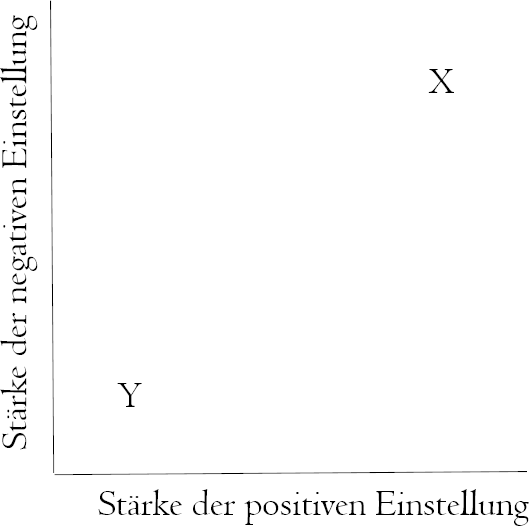
\includegraphics[scale=0.7]{ModellEinstellungen2D} 
\begin{tikzpicture}
    \begin{axis}[axis lines*=left,
                 xtick=\empty,
                 ytick=\empty,
                 ylabel={Stärke der negativen Einstellung},
                 xlabel={Stärke der positiven Einstellung},
                 ylabel near ticks,
                 xlabel near ticks,
                 nodes near coords,
                 point meta=explicit symbolic,
                 enlargelimits=0.25]
        \addplot [black, only marks] coordinates { (0,0) [Y] (1,1) [X] };
    \end{axis}
\end{tikzpicture}
\caption{Zweidimensionale Modellierung von Einstellungen \citep[s.][207]{Jonas.2014}}
\label{pic:2D}
\end{figure}

Es ist schwierig zu sagen, wie die einzelnen Komponenten von Einstellungen genau interagieren und welche Rolle sie jeweils spielen \citep[s.][400]{Lasagabaster.2005}. 
Da die Trennung der drei Komponenten sehr schwer aufrecht zu erhalten ist, wird sie sogar oft insgesamt kritisch gesehen~\citep[s. etwa][34]{Cuonz.2014}. 
Insbesondere was die Verhaltenskomponente von Einstellungen angeht, gibt es in der Forschung unterschiedliche Meinungen dar{\"u}ber, wie eng diese mit den beiden anderen Komponenten zusammenh{\"a}ngt \citep[s.][25]{Garrett.2012}. 
Einerseits kann ein bestimmtes Verhalten dazu führen, dass wir eine bestimmte Einstellung ausbilden, um zu verhindern, dass unser Verhalten und unsere Einstellungen nicht übereinstimmen \citep[s.][203]{Jonas.2014}. 
Andererseits kann aus starken Einstellungen unter bestimmten Voraussetzungen das Verhalten vorhergesagt werden \citep[s.][224--225]{Jonas.2014}. 
Ob eine Einstellung zu einem bestimmten Verhalten führt, hängt aber auch von der Motivation einer Person ab, das Verhalten tatsächlich auszuführen. 
Außerdem spielen die Erwartungen anderer eine Rolle sowie nicht zuletzt die eigene Einschätzung der Fähigkeit, das Verhalten auszuführen (\cites[s.][224--225]{Jonas.2014}[s. auch][]{Ajzen.1977}). 
Die positive Einstellung einer Person zum Dialekt führt also eher dazu, dass sie den Dialekt verwendet, wenn sie dazu motiviert ist, wenn andere von ihr erwarten, dass sie im Dialekt spricht, und wenn sie den Dialekt beherrscht. 
Die \textit{Theory of Reasoned Action} geht deshalb davon aus, dass eher Verhaltensabsichten als das Verhalten selbst Voraussetzung für die Einstellung sind~\citep[s.][26--27]{Garrett.2012}.\largerpage[-1]

Das Verhalten wird in der Sozialpsychologie aufgrund dieser recht komplexen Zusammenhänge nur unter bestimmten Voraussetzungen als Hinweis auf eine bestimmte Einstellung genutzt, n{\"a}mlich dann, wenn die anderen Einstellungskomponenten nur schwach ausgepr{\"a}gt sind oder wenn f{\"u}r ein Verhalten au{\ss}er der Einstellung keine andere Begr{\"u}ndung infrage kommt~\citep[s.][221]{Aronson.2014}. 
Dass es einen gewissen Zusammenhang zwischen Einstellung und Verhalten gibt, ist jedoch die theoretische Voraussetzung dafür, das Ausfüllen eines Fragebogens oder andere Reaktionen auf sprachliche Phänomene als Hinweise auf eine kognitive Einstellung zu deuten \citep[s.][401]{Lasagabaster.2005}.

\citet[78]{Hermanns.2002} zufolge ist die affektive Komponente die zentrale und wichtigste Einstellungskomponente. Auch \citet[222]{Cargile.1994} betonen die Zentralit{\"a}t von Emotionen. Bspw. halten sie es f{\"u}r unwahrscheinlich, dass die kognitive Komponente die affektive {\glqq}{\"u}berstimmt{\grqq} \citep[s.][222]{Cargile.1994}. 
Dies passt zu der Beobachtung, dass es nur sehr selten geschieht, dass affektive Einstellungen durch Argumente ver{\"a}ndert werden~\citep[s.][219]{Aronson.2014}. 
\citet[142]{Riehl.2000} definiert Einstellungen sogar als ausschließlich affektiv. 
Viele dieser Abgrenzungsschwierigkeiten basieren auf der Gleichsetzung der Einstellung selbst mit den Komponenten (s. oben). 
Sieht man diese jedoch wie \citet[]{Jonas.2014} als Voraussetzungen für Einstellungen, wird deutlich, dass bspw. die affektive Komponente keinesfalls allein entscheidend dafür ist, welche Einstellung jemand entwickelt, sondern dass auch die Verhaltenskomponente, vor allem aber das erworbene Wissen die Einstellung prägen.\footnote{Bspw. ist die Einschätzung \citeauthor{Riehl.2000}s (\citeyear[147]{Riehl.2000}), eine Probandin äußere mit ihrer Aussage \object{ich weiß es nicht warum [...] aber grad das heftige sächsisch [...] gefällt mir einfach nicht} eine \glqq rein affektive Zuweisung\grqq{} zu hinterfragen. Da \citet[159]{Riehl.2000} selbst Stereotype als \glqq kognitive Größen\grqq{} sieht, auf denen solche Spracheinstellungen beruhen, ist diese Schlussfolgerung nicht nachvollziehbar.}

Als weitere Schwierigkeit bei der Erforschung von Spracheinstellungen nennen \citet[182]{Plewnia.2011}, dass Einstellungen von den Befragten unterschiedlich stark reflektiert w{\"u}rden \citep[s. auch][143]{Riehl.2000}. 
Das heißt, Einstellungen können sowohl explizit als auch implizit vorhanden sein: 
\begin{quote}Explizite Einstellungen sind solche, die wir bewusst bekr{\"a}ftigen und {\"u}ber die [wir] leicht Auskunft geben k{\"o}nnen; sind das, was wir als unsere Bewertung angeben.~\citep[222]{Aronson.2014}\end{quote}
Implizite Einstellungen hingegen seien viel weniger kontrollierbar und häufig unbewusst \citep[s.][222]{Aronson.2014}. Wie die einzelnen Einstellungskomponenten können sich auch explizite und implizite Einstellungen widersprechen \citep[s.][222]{Aronson.2014}. Das heißt, jemand kann bspw. zwar eine explizit negative affektive Einstellung gegenüber Katzenvideos äußern, aber beim Anschauen dennoch positive Gefühle entwickeln, die eine andere implizite Einstellung verraten.

Die drei Komponenten, Affekt, Kognition und Konation, werden zwar als Voraussetzungen für (implizite und explizite) Einstellungen gesehen, können aber noch nicht erklären, wie es zu einer Einstellung kommt. 
Damit und mit der Frage, welche Aspekte (bspw. welche Gefühle und welche Art von Wissen) für die Herausbildung einer Spracheinstellung relevant sind, beschäftigt sich der folgende Abschnitt. 
\subsubsection{Bewertungsgrundlage und Bewertungskategorien}
\label{sec:Bewertungsgrundlage}
Zu der Frage, wie die Bewertung sprachlicher Formen zustande kommt, gibt es zwei Hypothesen: 
Die \textit{inherent value hypothesis} geht davon aus, dass bspw. phonologische Merkmale f{\"u}r die positive oder negative Bewertung von W{\"o}rtern oder Variet{\"a}ten verantwortlich sind, w{\"a}hrend die \textit{imposed norm hypothesis} davon ausgeht, dass soziale Stereotype und Konnotationen f{\"u}r die Bewertung sprachlicher Formen und Variet{\"a}ten verantwortlich ist~\citep[s.][5]{Garrett.2012}. 
Die erste Hypothese wird allerdings kaum vertreten, da sich gezeigt hat, dass sprachinterne Merkmale für die Bewertung nicht ausschlaggebend sind: 
\begin{quote}[I]t has been shown that listeners rating totally unfamiliar (foreign) varieties (which for respondents were non-categorizable socioeconomically) did not discriminate between them on the ground of aesthetic and status differences, although they were perceived to differ sharply in these qualities within their own speech communities. It seems therefore that evaluations of language varieties do not reflect either linguistic or aesthetic qualities so much as the social conventions within speech communities concerning the status and prestige associated with \so{speakers} of the varieties.~\citep[585, Hervorhebung im Original]{Giles.1988}\end{quote}
Die Bewertung sprachlicher Formen erklärt sich also aus deren Verknüpfung mit sozialen Werten, d.\,h., Spracheinstellungen stellen nicht in erster Linie Reaktionen auf formale Gegebenheiten, sondern 
\begin{quote}gesellschaftlich vermittelte Produkte sozialer Lernprozesse dar und sind als solche entwicklungsf{\"a}hig und ver{\"a}nderbar und in ihrer Aktualisierung von situationsspezifischen Bedingungen abh{\"a}ngig.~\citep[728]{Neuland.1993}\end{quote}
Spracheinstellungen werden also im Laufe der Sozialisation erlernt.\footnote{Man nimmt an, dass Einstellungen, die relativ fr{\"u}h erworben werden, verhältnismäßig stabil sind und nicht so leicht ge{\"a}ndert werden (\citealp[5]{Garrett2003}; s. auch \citealp[30]{Garrett.2012}).}
Dabei spielen Eltern, Freund:innen, Erziehung und Bildung eine wesentliche Rolle \citep[s.][400]{Lasagabaster.2005}.\footnote{Es gibt Studien, die davon ausgehen, dass auch genetische Dispositionen Einstellungen beeinflussen können \citep[s.][400]{Lasagabaster.2005}.} 
\citet[22]{Garrett.2012} sieht als zwei wesentliche Bereiche, aus denen sich Spracheinstellungen speisen, die pers{\"o}nliche Erfahrung und das soziale Umfeld, zu dem er auch die Medien z{\"a}hlt.
Durch sie werden stereotype Vorstellungen {\"u}ber Sprecher:innen vermittelt und mit einer Variante oder Variet{\"a}t in Verbindung gebracht (\cites[s.][180]{Gartig2010}[180]{Plewnia.2011}[37]{Preston2004}). 
Stereotype formen Spracheinstellungen also zu einem großen Teil. 
Ein Stereotyp kann mit \citet{Aronson.2014} verstanden werden als

\begin{quote} 
\sloppy
eine verallgemeinernde Annahme über eine Gruppe von Menschen, die praktisch all ihren Mitgliedern, unabhängig von tatsächlichen Unterschieden zwischen ihnen, dieselben charakteristischen Merkmale zuschreibt. \citep[476]{Aronson.2014} 
\end{quote} 
Stereotype führen zu prototypischen Vorstellungen von Vertreter:innen sozialer Gruppen wie \object{Medizinerinnen sind intelligent} \citep[s.][142]{Riehl.2000}.
Eine solche Annahme zu typischen Eigenschaften oder Verhaltensweisen wird (meist unbewusst) auf sprachliche Merkmale, bspw. Fachbegriffe, übertragen, sodass diese ausreichen, um stereotype Vorstellungen hervorzurufen (\cites[s.][81]{Hundt.1992}[38--39]{Preston2004}). 
Stereotype lassen sich der kognitiven Komponente zuordnen und sind wesentlich für die Herausbildung von Spracheinstellungen \citep[s.][201]{Jonas.2014}. 
Dabei spielen sowohl Heterostereotype, also Vorstellungen über andere Gruppen, als auch Autostereotype eine Rolle, also Vorstellungen über die eigene Gruppe \citep[s.][6--7]{Hundt.1992}. 
Hinzu kommen vermutete Hetero- und vermutete Autostereotype. 
\citet[7]{Hundt.1992} schreibt stereotypen Vorstellungen mehrere Funktionen zu, unter anderem Orientierung und Komplexitätsreduktion. 
Des Weiteren haben Stereotype immer auch eine Selbstdarstellungsfunktion:~Indem ich andere auf eine bestimmte Weise darstelle, positioniere ich mich selbst~\citep[s.][7]{Hundt.1992}. 
\citet[728]{Neuland.1993} f{\"u}hrt deshalb an, dass Spracheinstellungs{\"a}u{\ss}erungen mehr Aufschluss {\"u}ber die Person geben, die diese {\"a}u{\ss}ert, als {\"u}ber das Einstellungsobjekt, also etwa die Variet{\"a}t, da sie insbesondere zur Konstruktion der eigenen Identit{\"a}t und zur Abgrenzung von anderen dienen. 
Spracheinstellungen sind daher gruppenspezifisch \citep[s.][627]{Garrett.2001}. So zeigen \citet{Garrett.1999} etwa, dass walisische Jugendliche andere Einstellungen gegenüber der \textit{Received Pronunciation} (RP) haben als ihre Lehrer:innen. 

Die Bedeutung sozialer Gegebenheiten für Spracheinstellungen schlägt sich in den Kategorien nieder, die bei der Bewertung sprachlicher Merkmale relevant gemacht werden.  
So zeigt sich in bisherigen Studien, dass die wichtigsten Bewertungsaspekte sich in eine Status- und eine Wärmekategorie aufteilen (\cites[s.][155]{Creber.1983}[49]{Preston2004}{Fiske.2002}). 
Zur Statuskategorie gehören Eigenschaften wie Kompetenz und Bildung;  
Eigenschaften wie Freundlichkeit, Gruppensolidarität und Sympathie werden in der Wärmekategorie zusammengefasst~\citep[s.][182]{Plewnia.2011}.
\citet[223--224]{Cargile.1994} nennen zahlreiche Studien, die Evidenz f{\"u}r solche unterschiedlichen Bewertungsdimensionen liefern, wobei nicht immer die gleichen Dimensionen festgestellt werden. \citet{Lambert.1967} etwa unterscheidet zwischen \textit{personal integrity, competence} und \textit{social attractiveness}; 
\citet[117]{Garrett.2007} nennt \textit{superiority, social attractiveness} und \textit{dynamism}. 
Häufig lässt sich ein Zusammenspiel zwischen einer positiven Bewertung in der einen Dimension und einer negativen Bewertung in der anderen Dimension beobachten, sodass Gruppen und die ihnen zugeschriebenen sprachlichen Merkmale entweder als freundlich, sympathisch usw., aber wenig kompetent oder aber als gebildet und professionell, aber unsympathisch empfunden werden \citep[s.][878--879]{Fiske.2002}.
Bei der Bewertung von Variet{\"a}ten zeigt sich als Muster, dass Sprecher:innen die eigene  Nonstandardvariet{\"a}t freundlich, sympathisch und vertrauensw{\"u}rdig, aber langsam und wenig intelligent finden, w{\"a}hrend sie Sprecher:innen der Standardvarietät als kalt, unehrlich, unsympatisch und intelligent empfinden~\citep[s.][1687]{Preston2005}.
% Änderung Anfang
F{\"u}r die Bewertung in Kategorien wie Kompetenz und Bildung ist dabei entscheidend, wie der gesellschaftliche Status der bewerteten Gruppe eingesch{\"a}tzt wird:~Gilt er als hoch, werden Gruppenmitglieder als professionell und kompetent wahrgenommen~\citep[897]{Fiske.2002}.
Die Bewertung in der Wärmedimension hängt \citet[897]{Fiske.2002} zufolge maßgeblich davon ab, ob die bewertete Gruppe als Konkurrenz bzw. als Gefahr für den eigenen Status empfunden wird.
Positive Werte in Status- und Wärmedimension erhalten neben der eigenen \textit{In-Group} insbesondere Gruppen, die in einer Gesellschaft als Referenzgruppe gelten; in den USA bspw. gilt dies laut \citet[898]{Fiske.2002} etwa für die Mittelschicht.
% Änderung Ende

Dass soziale Kategorien die entscheidenden Aspekte der Bewertung sind, heißt allerdings nicht, dass immer bewusst auf diese referiert wird. 
Vordergründig stehen häufig andere Kriterien im Zentrum. 
So zeigt \citeauthor{Preston2004} (\citeyear{Preston1996, Preston2004, Preston2005}), dass sich Befragte vor allem auf die Kategorien Korrektheit und angenehmer Klang beziehen. 
Über die Korrektheit als Bewertungskategorie schreibt er: {\glqq}I personally believe it is no exaggeration to say that it may be the most powerful contributor to awareness in American English{\grqq}~\citep[54]{Preston1996}. 
Solche normativen oder ästhetischen Kriterien sind allerdings eng mit sozialen Kategorien assoziiert. 
Bspw. werden Sprecher:innen der Standardvarietät in Statuskategorien wie Intelligenz h{\"o}her bewertet, w{\"a}hrend Sprecher:innen einer Nonstandardvariet{\"a}t eher bei Eigenschaften wie Vertrauensw{\"u}rdigkeit h{\"o}her bewertet werden~(\citealp[s.][155]{Creber.1983}; sowie \autoref{sec:Prestigevarietaet}). 
Auch \citet[732]{Neuland.1993} stellt fest, dass die Bewertung eines Merkmals als nicht normgerecht h{\"a}ufig mit der Bewertung desselben Merkmals als sympathisch korreliert. 
Auf der anderen Seite kann die Standardvarietät in bestimmten Situationen mit geringer Solidarität assoziiert sein \citep[s.][586--587]{Giles.1988}.

Vor dem Hintergrund dieser Befunde zum Zustandekommen von Spracheinstellungen lässt sich mehr über deren Funktion sagen. 
In der Sozialpsychologie wird zwischen Objekten unterschieden, die eher aufgrund ihres Nutzens beurteilt werden (etwa Klimaanlagen) und Objekten, deren Bewertung auf sozialen Werten beruht (etwa Nationalflaggen) \citep[s.][210]{Jonas.2014}. 
Sprache lässt sich klar dem letzteren Gegenstandstyp zurechnen. 
Ihre Bewertung betrifft die eigene Identität und persönliche Werte: 
\begin{quote} A speaker's language attitudes mirror the norms of the group of people to whom he/she relates most closely, especially when these attitudes and the behaviour which they guide function as group identity markers. This implies that language behaviour has social meaning and prompts social categorization. \citep[1321]{Vandermeeren2005} \end{quote} 
Somit wird deutlich, dass Spracheinstellungen zwar als kognitive Phänomene konzeptualisiert werden können, sich aber nicht losgelöst vom sozialen Kontext betrachten lassen. 
Dies wird im folgenden Abschnitt weiter ausgeführt. 
\subsubsection{Spracheinstellungen im Kontext}
\label{sec:Interaktion}
\citet[72--73]{Hermanns.2002} kritisiert an der sozialpsychologischen Theorie der Einstellungen, dass nicht zwischen abstrakten Typen von Einstellungen und gerade aktualisierten unterschieden wird:
\begin{quote}Ausgelassen bleibt an dieser Stelle der Gedanke, dass man eine virtuelle Einstellung immer erst noch aktualisieren muss, damit sie wirksam sein kann. Wie auch der Gedanke, dass es durchaus aktuelle Bereitschaften zu Arten des Reagierens geben kann, die keinem Typ der gelernten Einstellungen entsprechen.~\citep[73]{Hermanns.2002}\end{quote}
In diesem Zusammenhang weist er auch darauf hin, dass Menschen oft verschiedene Einstellungen ein und derselben Sache gegen{\"u}ber haben, also {\"u}ber Einstellungssets verf{\"u}gen. 
Welche Einstellung aktualisiert % Änderung Anfang
und geäußert % Änderung Ende
wird, h{\"a}ngt dann ma{\ss}geblich vom Kontext ab \citep[73--74]{Hermanns.2002}. 
Entgegen dieser Kritik wird die Kontextabhängigkeit von Einstellungen in der Sozialpsychologie und in der Spracheinstellungsforschung bereits berücksichtigt. 
\citet[210--211]{Jonas.2014} etwa gehen darauf ein, dass die Äußerung einer Einstellung davon abhängig sein kann, wem gegenüber sie getätigt wird. 
Auch wie sich eine Testperson f{\"u}hlt, kann sich auf ihre Einstellungen auswirken~\citep[s.][218]{Cargile.1994}. 

Neuere Arbeiten der Spracheinstellungsforschung betonen, dass Spracheinstellungen in der Interaktion entstehen (\cites[s.][205--206]{Tophinke.2006}[200]{Liebscher.2009}[5--6]{Konig.2014}). \citet{Konig.2014} etwa untersucht Spracheinstellungsäußerungen in konkreten Interaktionen und zeigt, wie metapragmatisches Wissen -- etwa über die Angemessenheit sprachlicher Formen~-- ausgehandelt wird (\cites[s. auch][200]{Konig2015}{Konig.2017}). 
Anhand von Interviewausschnitten zum Sächsischen demonstrieren \citet[206--207]{Liebscher.2009}, dass es sich bei % Änderung Anfang
Spracheinstellungsäußerungen % Änderung Ende
um Positionierungen in den sozialen Strukturen einer konkreten Situation handelt. 
Die Interviewteilnehmer:innen gehen durch ihre Äußerungen etwa in Opposition zu anderen Beteiligten. 
\citet[218]{Liebscher.2009} kommen zu dem Schluss, dass es kontextunabhängige Einstellungen nicht geben kann. 

Auch ältere Studien im Bereich der Spracheinstellungen sehen bereits die Relevanz des Kontextes.
Ein Beispiel ist eine Untersuchung von \citet{Creber.1983}, in der zwölf- bis 14-jährige britische Schüler:innen Standard- und Nonstandardsprecher:innen in einem informellen und einem formellen Setting bewerten sollen. 
Es zeigt sich, dass positive Statuseigenschaften noch stärker mit der Standardvarietät verbunden werden, wenn die Bewertung innerhalb eines formellen Settings stattfindet \citep[s.][159]{Creber.1983}.

In einer nat{\"u}rlichen Interaktionssituation dient nicht nur die Sprache einer Sprecherin als Bewertungsgrundlage, sondern der H{\"o}rer bezieht in sein Urteil auch bspw. die Kleidung, das Auftreten usw. mit ein. 
Sprachliche Merkmale sind in der Interaktion allerdings besonders relevant: \begin{quote} Indeed, contextual issues notwithstanding, we maintain that language behaviours are among the most salient and often used cues in social interaction, and thus the importance of focusing on language attitudes~\citep[215]{Cargile.1994} \end{quote}
Das bereits gewonnene Wissen über ein Gegenüber beeinflusst die Interpretation der sprachlichen Merkmale aber erheblich. 
\citet{Cargile.1994} modellieren die gemeinsame Vergangenheit der Interaktionspartner:innen daher als eine Art Filter, der die Reaktion auf ein sprachliches Verhalten mitbestimmt. 
Spricht bspw. eine gute Freundin mit einem bestimmten Akzent, der sonst als ungebildet empfunden wird, ist diese Interpretation nicht wirksam, wenn die Freundin als intelligent eingesch{\"a}tzt wird \citep[s.][222--223]{Cargile.1994}. 
Auch dies betont die Kontextabh{\"a}ngigkeit von Spracheinstellungen.

%\begin{figure}\includegraphics[width=\textwidth]{Images/Cargile,Gilesetal(2).jpg}\caption{Spracheinstellungsmodell von \citet[214]{Cargile.1994}}
%\label{pic:Cargile}
%\end{figure}
Spracheinstellungen % Änderung Anfang
und die Äußerungen, zu denen sie führen, % Änderung Ende
sind also keineswegs nur kognitiv, sondern insbesondere sozial bedingt, was auch \citet{Aronson.2014} betonen. 
Sie bezeichnen Einstellungen als {\glqq}hochgradig soziales Ph{\"a}nomen, das vom angenommenen oder tats{\"a}chlichen Verhalten anderer Menschen beeinflusst wird{\grqq}~\citep[223]{Aronson.2014}. 
\citet{Garrett.2012} schließt daher:
\begin{quote}[L]anguage attitudes issues extend to all manner of sociolinguistic and social psychological phenomena, such as how we position ourselves socially, and how we relate to other individuals and groups. They may affect behaviours and experiences.~\citep[15]{Garrett.2012}\end{quote}
Spracheinstellungsäußerungen sind damit nicht nur zu einem wesentlichen Teil vom Kontext abhängig, sondern sie wirken auch auf diesen zurück. 
In Interaktionssituationen werden Spracheinstellung% Änderung Anfang
säußerungen und damit auch die Einstellungen selbst % Änderung Ende
daher sowohl als Input als auch als Output gesehen, wie bereits oben in der Diskussion des Zusammenhangs von Verhalten und Einstellungen angeklungen ist (s. \autoref{sec:Komponenten}; \citealp[400]{Lasagabaster.2005}). 
Als Beispiel nennt \citet[21]{Garrett.2012} Einstellungen gegen{\"u}ber dem Walisischen:~Auf der einen Seite k{\"o}nnen positive Einstellungen dazu f{\"u}hren, dass das Walisische erlernt wird (Input), auf der anderen Seite kann das erfolgreiche Erlernen der Sprache zu positiven Einstellungen f{\"u}hren (Output). 
Das bedeutet, dass Spracheinstellungen soziale Realität mitformen. 
Dies zeigt bspw. auch eine Untersuchung von \citet{Keim.1995}, in der es darum geht, wie das sprachliche Verhalten und die Identifikation mit einer lokalen Gemeinschaft zusammenhängen. 
In Narrativen der Proband:innen \citeauthor{Keim.1995}s werden verschiedene Variet{\"a}ten (Dialekt und Standard) zur Konstruktion einer wir-Gruppe in Abgrenzung zu einer fremden, negativ bewerteten Gruppe (bspw. die Vornehmen) verwendet~\citep[s.][170]{Keim.1995}.

Mit dieser Hinwendung zu konstruktivistischen Fragestellungen nähert sich die Spracheinstellungsforschung der Sprachideologieforschung an, deren anthropologisch geprägte Theorie darauf ausgerichtet ist, dem Zusammenhang von sprachlichen und sozialen Kategorien auf den Grund zu gehen. 
\subsection{Sprachideologieforschung}
\label{sec:Sprachideologieforschung}
Der Begriff Ideologie ist in der Alltagssprache meist negativ konnotiert \citep[s.][124--127]{Silverstein1998}. Ideologien werden häufig verstanden als \glqq a system of wrong, false, distorted or otherwise misguided beliefs, typically associated with our social or political opponents\grqq{} \citep[2]{vanDijk.1998}. 
Der anthropologische Ideologiebegriff hingegen meint nicht etwa falsche Vorstellungen, sondern schließt alle Konzeptualisierungen, auch wissenschaftliche, mit ein (\cites[s.][312]{Silverstein1992}[124]{Silverstein1998}). 
Ideologien werden hier urteilsfrei als Systeme von Annahmen und Wertungen gefasst (\cites[s.][3]{vanDijk.1998}[12]{Gal.2019}).\footnote{Die einzelnen Ansätze unterscheiden sich hier durchaus, wie \citet[56--57]{Woolard1994} herausstellen: Während einige grundsätzlich alle Konzeptualisierungen als ideologisch auffassen (hier nennen \citeauthor{Woolard1994} etwa \citealp{Rumsey.1990}), stellen andere die Gefahr der ideologisch verzerrten Darstellung in den Vordergrund und betrachten Ideologien in erster Linie als Mittel, soziale Privilegien zu rechtfertigen.} 
Bei Ideologien handelt es sich um gesellschaftliche Phänomene, das heißt, sie sind immer in einer bestimmten Gruppe verortet und hängen eng mit deren Kultur zusammen (\cites[s.][312]{Silverstein1992}[3]{vanDijk.1998}).

Sprachideologien sind demzufolge Wertehaltungen und Grundeinstellungen einer Gesellschaft zu Sprache und sprachlichen Formen (\cites[s.][]{Silverstein1979}{Silverstein1992}{Silverstein1998}{Kroskrity.2010}{Spitzmuller2013}). 
\citet[193]{Silverstein1979} definiert sie als \glqq any sets of beliefs about language articulated by the users as a rationalization or justification of perceived language structure and use\grqq{}. 
Anders als der sozialpsychologisch geprägten Spracheinstellungsforschung geht es der Sprachideologieforschung also nicht um kognitive Repräsentationen, sondern es wird untersucht, auf welchen grundlegenden Annahmen über Sprache metapragmatische Äußerungen beruhen \citep[s.][223]{Silverstein.1985}. 
Diese sprachideologischen Annahmen können aus expliziten metapragmatischen {\"A}u{\ss}erungen abgeleitet werden, kommen aber noch h{\"a}ufiger implizit zum Ausdruck, indem in bestimmter Weise auf einen Sprachgebrauch reagiert wird~\citep[s.][116]{Gal.2016}.

\begin{sloppypar}
Sprachideologien werden zumindest von einer Gruppe innerhalb einer Sprechergemeinschaft oder aber sogar von der ganzen Sprechergemeinschaft geteilt \citep[s.][125]{Silverstein1998}. 
Welche Sprachideologien in einer Gesellschaft entwickelt und verbreitet werden, h{\"a}ngt dabei zu einem Teil auch davon ab, wie das Sprachsystem aufgebaut ist~\citep[s.][194]{Silverstein1979}. 
Bspw. setzt ein Diskurs über gendergerechte Sprache ein Sprachsystem voraus, in dem die Markierung verschiedener Geschlechter angelegt ist. 
\end{sloppypar}

\begin{sloppypar}
Dass Sprachideologien gesellschaftliche Phänomene sind, zeigt sich daran, dass es im Wesentlichen um den in einer Gruppe angenommenen \glqq Zusammenhang zwischen sprachlicher Variation bzw. Sprachwahl auf der Mikroebene und gesellschaftlich\hyp sozialer Differenzierung auf der Makroebene\grqq{}~\citep[202]{Konig2015} geht. 
Sprachideologien sind also als Verbindungen zwischen sprachlichen Formen und sozialen Strukturen zu verstehen \citep[s.][55]{Woolard1994}. 
Dabei ist wichtig, dass weder die sprachlichen noch die sozialen Kategorien als von sich aus gegeben angenommen werden:
Zum einen sind Sprachideologien entscheidend dafür, wie Sprache konzeptualisiert und kategorisiert wird. 
Zum anderen werden soziale Strukturen und Identit{\"a}ten erst durch (sprachliche) Interaktion und Ideologien darüber konstruiert (\cites[s.][289]{Ochs.1993}[407]{Ochs1996}[70]{Eckert.2016}). 
Ideologien über Sprache wirken daher mit an der Konstruktion sozialer Realität, indem sie sprachliche Formen und Varietäten mit bestimmten Sprecher- oder Kontextmerkmalen verbinden und dadurch spezifische Gruppen oder Situationen häufig erst konstituieren: 
\end{sloppypar}

\begin{quote}[I]t has become clearer that people not only speak about, or refer to, the world “out there” -- outside of language -- they also presuppose (or reflect) and create (or fashion) a good deal of social reality by the very activity of using language.~\citep[194]{Silverstein1979}\footnote{\citeauthor{Silverstein1979} spricht daher nicht von Mikro- und Makroebene, sondern legt den Fokus darauf, wie Kultur diskursiv hervorgebracht wird \citep[s. etwa][]{Silverstein.2013}.}\end{quote}
Soziale Kategorien existieren also nicht losgelöst von Sprache und Vorstellungen darüber, wie Sprache verteilt ist \citep[s.][81--82]{Cameron.1990}. 
Der Zusammenhang zwischen sozialen Identit{\"a}ten und sprachlichen Formen ist dabei immer über Ideologien vermittelt~\citep[s.][288]{Ochs.1993}. 
Für diesen mittelbaren Zusammenhang zwischen Sprache und sozialer Realität spielt die Indexikalität sprachlicher Zeichen eine wesentliche Rolle. Dieses zentrale Konzept der Sprachideologie- oder Metapragmatikforschung ist Thema des folgenden Abschnitts. 

\subsubsection{Indexikalität}
\label{sec:Indexikalitaet}
Sprachliche Variation bietet Sprecher:innen die M{\"o}glichkeit, sich in einer konkreten Situation f{\"u}r eine Variante zu entscheiden. 
Damit ist die Voraussetzung dafür gegeben, diese Entscheidung sprachideologisch zu begründen und die Varianten so sozialsymbolisch aufzuladen~(\citealp[s. u.\,a.][]{Silverstein1979, HessLuttich2005, Eckert2008, Spitzmuller2013}). 
Bspw. werden unterschiedliche Stile oder Varianten oft vereinfachend spezifischen Gruppen zugewiesen und somit auf soziale Unterschiede zur{\"u}ckgef{\"u}hrt. 
In der Folge wird die Nutzung dieser Stile oder Varianten als Hinweis auf die Zugehörigkeit zu der damit assoziierten Gruppe interpretiert. 
Varianten k{\"o}nnen auf diese Weise als Marker sozialer Identität, etwa als weiblich, alt oder Akademikerin fungieren:
\begin{quote} It has become a commonplace in sociolinguistics that linguistic forms, including whole languages, can index social groups. As part of everyday behavior, the use of a linguistic form can become a pointer to (index of) the social identities and the typical activities of speakers.~\citep[36]{Irvine2000}\end{quote}
Indem eine bestimmte Variante verwendet wird, wird also etwas {\"u}ber die soziale Identit{\"a}t ausgesagt -- entweder über die eigene oder über die derjenigen Person, der die Variante in den Mund gelegt wird~\citep[s.][222]{Silverstein.1985}. 
Diese sozialsymbolische Verweiskraft, also \glqq die Fähigkeit sprachlicher Zeichen, soziale Werte, Akteurstypen und Lebensformen zu evozieren bzw. zu kontextualisieren\grqq{} \citep[265]{Spitzmuller2013}, wird in der Sprachideologieforschung als Indexikalität bezeichnet \citep[s.][]{Silverstein1979,Silverstein2003}.\footnote{Unter der Indexikalität sprachlicher Zeichen wird nicht nur der Verweis auf außersprachliche Merkmale verstanden, sondern auch der Verweis auf den Kotext \citep[s.][6--8]{Auer.1995}. \citet[42]{Auer.1989} spricht bei Verweisen auf Außersprachliches von der exophorischen Indexikalität und unterscheidet diese von der endophorischen Indexikalität, womit z.\,B. gemeint ist, dass Wörter durch ihre Endungen auf kongruente Wörter verweisen.}
Dabei kann unterschieden werden zwischen der indexikalischen Form, die in einem sprachlichen Merkmal besteht, dem eine verweisende Kraft zugeschrieben wird, und dem \textit{indexed feature}, einem Kontextmerkmal, auf das verwiesen wird \citep[s.][2]{Auer.1995}.

Die soziale Bedeutsamkeit der Variation sprachlicher Zeichen sollte nicht als bloßer Nebenschauplatz verstanden werden: 
Sie ist ein wesentliches Element von Sprache und häufig zentral für den Ablauf der Kommunikation (\cites[s.][19]{Silverstein.1976}[131]{Gumperz.1982}[68]{Eckert.2016}).\footnote{Während in der Sprachideologieforschung v.\,a. von \textit{Indexikalität} die Rede ist, ist in anderen Teildisziplinen eher der von \citet{Gumperz.1982} geprägte Begriff der \textit{Kontextualisierung} geläufig.}
Ob man bei der Bestellung im Restaurant bspw. den Ausdruck \object{Radler} oder \object{Alster} verwendet, macht nicht nur auf der formalen Ebene einen Unterschied, sondern die Wahl der Variante wird vom Gegenüber als Zeichen der regionalen Herkunft interpretiert. 
Den Zeichengebrauch einer Person als indexikalisch zu interpretieren bedeutet jedoch nicht, eine Intentionalität zu unterstellen \citep[s.][78]{Eckert.2016}. 
Da Sprachideologien meist nicht reflektiert werden, geschieht die Wahl einer Variante in den meisten Fällen unbewusst. 
Möglich ist auch, dass eine Form zun{\"a}chst bewusst eingesetzt wird und dann mit der Zeit in einen automatischen Gebrauch {\"u}bergeht~\citep[s.][79]{Eckert.2016}.

Jedes formale Merkmal einer Sprache kann theoretisch indexikalisch aufgeladen werden (\cites[s.][42]{Silverstein.1976}[206]{Silverstein1979}). 
Dabei können zwei Typen indexikalischer Tokens unterschieden werden: solche, bei denen die indexikalische Bedeutung Teil der Denotation ist, wie etwa Deiktika, und solche, bei denen die Denotation unabhängig von der Indexikalität ist (\cites[s.][34]{Silverstein.1976}[497]{HessLuttich2005}).\footnote{\citet[3]{Auer.1995} weist darauf hin, dass häufig lediglich diejenigen indexikalischen Zeichen in den Fokus der pragmatischen Linguistik gerückt wurden, deren Denotation ohne die Berücksichtigung des Kontextes nicht bestimmt werden kann.}
Letzteres wird besonders gut an Wortpaaren wie \object{Personenkraftwagen} und \object{Auto} deutlich, die zwar die gleiche Denotation aufweisen, denen aber unterschiedliche Indexikalitäten zugeschrieben werden. 
\citet[30--31]{Silverstein.1976} nennt als Beispiel Sexusmarker der Muskogee-Sprachen, die anzeigen, ob eine Aussage von einer Sprecherin oder einem Sprecher ge{\"a}u{\ss}ert wird.
Ein weiteres Beispiel sind die lange und kurze Genitivendung im Deutschen (\object{Baums/Baumes}): Beide tragen die gleiche grammatische Bedeutung, die lange Endung ist aber mit mehr Prestige aufgeladen \citep[s.][]{Szczepaniak2014}.\footnote{Prestige kann mit \citet{Strasser2005} verstanden werden als {\glqq}die Wertschätzung, die einer Person oder Gruppe aufgrund von positiv bewerteten Eigenschaften, wie berufliche Position oder Clubmitgliedschaft, entgegengebracht wird{\grqq}~\citep[412]{Strasser2005}. Stigma bezeichnet komplementär dazu die Abwertung einer Gruppe oder Person \citep[s.][412]{Strasser2005}.}
Solche Zeichen verfügen neben ihrer inhaltsseitigen Bedeutung über davon unabhängige, indexikalische Bedeutungsaspekte, die sich bspw. auf die Kontexte beziehen, in denen sie verwendet werden, oder auf Sprechertypen, mit denen sie assoziiert sind~\citep[s.][206--207]{Silverstein1979}. 
Hier trägt die indexikalische Funktion des Zeichens nicht zur Proposition bei, sondern operiert auf der Ebene des Kontextes. 

\textcites[33--35]{Silverstein.1976}[195--196]{Silverstein2003} beschreibt zwei Seiten der Indexikalität einer Form, die er \textit{presupposition} und \textit{entailment}\footnote{Anstatt von \textit{entailment} spricht \citeauthor{Silverstein1979} z.\,T. auch von \textit{creativity} oder von einem kreativen Effekt (\cites[s.][]{Silverstein.1976}[]{Silverstein1979}).} nennt: 
Mit \textit{presupposition} ist gemeint, dass eine Form bestimmte Kontextmerkmale voraussetzt. 
Ihr Auftreten und ihr Verständnis sind nur möglich, wenn bestimmte Voraussetzungen erfüllt sind. 
Deutlich wird dies insbesondere bei indexikalischen Zeichen, die nur mithilfe des Kontextes interpretierbar sind, wie etwa deiktische Ausdr{\"u}cke (bspw. \object{dieses} in \object{probier mal dieses Kabel})~\citep[s.][33]{Silverstein.1976}. 
Damit geht es bei der \textit{presupposition} auch um die Angemessenheit eines Zeichens im bis zu diesem Punkt etablierten Kontext \citep[s.][195]{Silverstein2003}. 

Der Begriff des \textit{entailment} zielt darauf ab, dass durch die Verwendung einer  Form in einer Situation die Merkmale des Kontextes erst sichtbar gemacht werden. Hier geht es um die Wirkung des Zeichens im Kontext:

\begin{quote} In some cases, the occurrence of the speech signal is the only overt sign of the contextual parameter, verifiable, perhaps, by other, cooccurring behaviors in other media, but nevertheless the most salient index of the specific value. Under these circumstances, the indexical token in speech performs its greatest apparent work, seeming to be the very medium through which the relevant aspect of the context is made to “exist.” \citep[34]{Silverstein.1976}
\end{quote}
Bspw. kann die Äußerung \object{wenn du alles aufisst...} je nach Intonation entweder als Drohung oder als Äußerung einer Bedingung aufgefasst werden. 
Die Intonation verweist also indexikalisch auf eine bestimmte Praktik und kann über diese Indexikalität zu einer bestimmten Interpretation führen \citep[s.][421]{Ochs1996}. 

Für das \textit{entailment} des indexikalischen Zeichens ist entscheidend, welche Implikationen die Verwendung im zuvor etablierten Kontext mit sich bringt \citep[s.][195]{Silverstein2003}. 
So könnte ein umgangssprachlicher Ausdruck in einem Vortrag humoristisch wirken, in einer anderen Situation unter Umständen aber als unhöflich empfunden werden. 
Die Verwendung einer indexikalischen Form wirkt sich außerdem wiederum auf die Erwartbarkeit und Angemessenheit anderer Zeichen aus. 
In einer E-Mail, die man aufgrund einer förmlichen Anrede und eines offiziellen Inhalts als formell wahrnimmt etwa, erwartet man eine Abschiedsformel wie \object{mit freundlichen Grüßen}. 
Diese Erwartungshaltung wird metapragmatisch verhandelt und durch Sprachideologien gestützt \citep[s.][196]{Silverstein2003}. 

Wichtig ist also, dass nicht davon ausgegangen werden kann, dass Kontext oder Kotext das Auftreten eines Zeichens determinieren, sondern dass die Wahl oder Nichtwahl eines Zeichens auch zur Kontextualisierung, also zur Gestaltung des Kontextes beiträgt (\cites[s.][23]{Auer.1986}[42--43]{Gumperz.1992b}).\footnote{In der Soziolinguististik wurde nichtsdestotrotz lange Zeit ein deterministischer Ansatz verfolgt und versucht, von einem Zeichen auf seine Benutzer:innen zu schließen \citep[s.][88--90]{Eckert2012}.
Unterschiede in der Variantenwahl wurden mit höherem bzw. geringerem Planungsaufwand oder mit sozialer Herkunft erklärt \citep[vgl. etwa die Kaufhausstudie von][]{Labov2006}.
\citet{Eckert2012} macht drei Phasen der variationslinguistischen Forschung aus und zählt Studien wie die \citeauthor{Labov2006}s zur ersten Phase.
Studien der zweiten Phase hingegen verfolgten einen ethnografischen Ansatz und berücksichtigten sprachideologische Fragestellungen, hielten sich aber immer noch an vorgefertigte Kategorien wie soziale Klasse \citep[s.][93]{Eckert2012}. Die dritte Phase schließlich brachte eine Fokussierung auf die stilistischen Praktiken der Sprachbenutzer:innen und deren sich wandelnde sozialsymbolische Bedeutungen, betont also die Agentivität der Sprecher:innen.} 
Variation wird damit als komplexes Zeichensystem verstanden \citep[s.][92]{Eckert2012}.
Für die Sprachideologieforschung und die Theorie der Indexikalität ist diese konstruktivistische Sichtweise zentral.

Wie oben bereits erwähnt, entsteht die indexikalische Bedeutung einer Variante nicht ad hoc, sondern wird in der Interaktion ausgehandelt. 
Beide Seiten des {in\-dexi\-ka\-li\-schen} Zeichens (also das bilaterale Zeichen aus Form- und Funktionsseite und die Kategorie, auf die dieses indexikalisch verweist) existieren zunächst unabh{\"a}ngig voneinander und werden erst über den metapragmatischen Diskurs verbunden (\cites[s.][316]{Silverstein1992}[86]{Jaffe.2016}). 
Sobald eine Variante metapragmatisch reflektiert wird, können ihr indexikalische Bedeutungen zugeschrieben werden.\footnote{Diese Zuschreibung sozialer Bedeutsamkeit zu einem zuvor als auffällig wahrgenommenen Merkmal entspricht dem, was \citeauthor{Purschke2014} unter Pertinenz fasst (s. \autoref{sec:MetapragmatischeBewusstheit}). Er betrachtet daher den {\glqq}Gegenstand von Hörerurteilen über Sprache [...] als die salienz- und pertinenzbasierte sozio-pragmatische Indexikalität lebensweltlicher Phänomene{\grqq}\citep[44]{Purschke2014}.} 
Auf diese Weise schaffen Sprachideologien Verbindungen zwischen sozialen Strukturen und sprachlichen Formen \citep[s.][55]{Woolard1994}. 
Dieser Prozess, in dem Formen bestimmte Bedeutungen zugeordnet werden, lässt sich mit \citet[86]{Jaffe.2016} als Indexikalisierung beschreiben und hängt eng zusammen mit dem Prozess der Registrierung \citep[s.][]{Agha2007}, auf den weiter unten eingegangen wird.

\citeauthor{Silverstein1979} (u.a. \citeyear{Silverstein1979}, \citeyear{Silverstein2003}) spricht von verschiedenen aufeinanderfolgenden indexikalischen Stufen bzw. Ordnungen (s. \autoref{pic:Indexikalitaet}). 
Auf der ersten Stufe (\textit{first-order-indexicality}) befinden sich Varianten, deren gruppen-, varietäten- oder registerspezifische Distribution zwar empirisch beobachtbar, den Sprecher:innen aber nicht bewusst ist \citep[s.][265]{Spitzmuller2013}.
Der Bezug der sprachlichen Form zu außersprachlichen Gegebenheiten bleibt hier von der Sprachgemeinschaft unbemerkt und ließe sich lediglich etwa durch Korpusuntersuchungen feststellen.
Auf der zweiten Stufe (\textit{second-order-indexicality}) stehen Varianten, die von Sprecher:innen als Kontextualisierungshinweise im Sinne \citeauthor{Gumperz.1982}' (\citeyear{Gumperz.1982}; s. auch \citealp{Auer.1986}) wahrgenommen werden. 
Kontextualisierungshinweise helfen Teilnehmer:innen einer Interaktion, zu interpretieren, {\glqq}what the activity is, how semantic content is to be understood and \textit{how }each sentence relates to what precedes or follows{\grqq}~\citep[131, Hervorhebung im Original]{Gumperz.1982}. 
Von Seiten der Sprachbenutzer:innen wird dabei häufig auch eine quantitative Verteilung angenommen, die durch außersprachliche Gegebenheiten gesteuert ist und dadurch auf diese verweist \citep[s.][266]{Spitzmuller2013}. 

Auf der Stufe der dritten indexikalischen Ordnung (\textit{third-order-indexicality}) entspricht das Zeichen einem Labovschen Stereotyp\footnote{\citet[52]{Silverstein.2016} weist selbst darauf hin, dass die Unterscheidung \citeauthor{Labov1963}s auf die Idee der indexikalischen Ordnungen übertragbar ist.}, das sich zur Stilisierung bestimmter Personengruppen oder kommunikativer Praktiken eignet (\cites[s.][308--309]{Labov1978}[220]{Silverstein2003}[92]{Eckert2012}). 
So wird etwa die Koronalisierung von [ç] bspw. in \object{ich} oder \object{dich} als ein typisches Merkmal in Äußerungen jugendlicher Sprecher:innen aus einem multikulturellen, großstädtischen Milieu gesehen und dazu verwendet, diese Gruppe zu konstruieren und stereotyp darzustellen (\cites[s.][]{Androutsopoulos.2011}[11]{Auer2014}). 
\citet[523]{Harnisch.2005} sieht insbesondere in morphologischen Varianten ein großes Potenzial, als soziale Marker genutzt zu werden. 
Er nennt etwa verbalmorphologische Klammergef{\"u}ge des unterfr{\"a}nkischen Dialekts (\textit{nei-lass-fall} \glq hineinfallen lassen\grq), dessen Sprecher:innen wegen dieses auff{\"a}lligen Merkmals teilweise mit Bildungen wie \textit{foto-lass-grafieren }verspottet werden, oder genderneutrale Partizipialformen wie \textit{Studierende}, die f{\"u}r politische Korrektheit und Feminismus stehen~\citep[s.][524]{Harnisch.2005}.

\begin{figure}
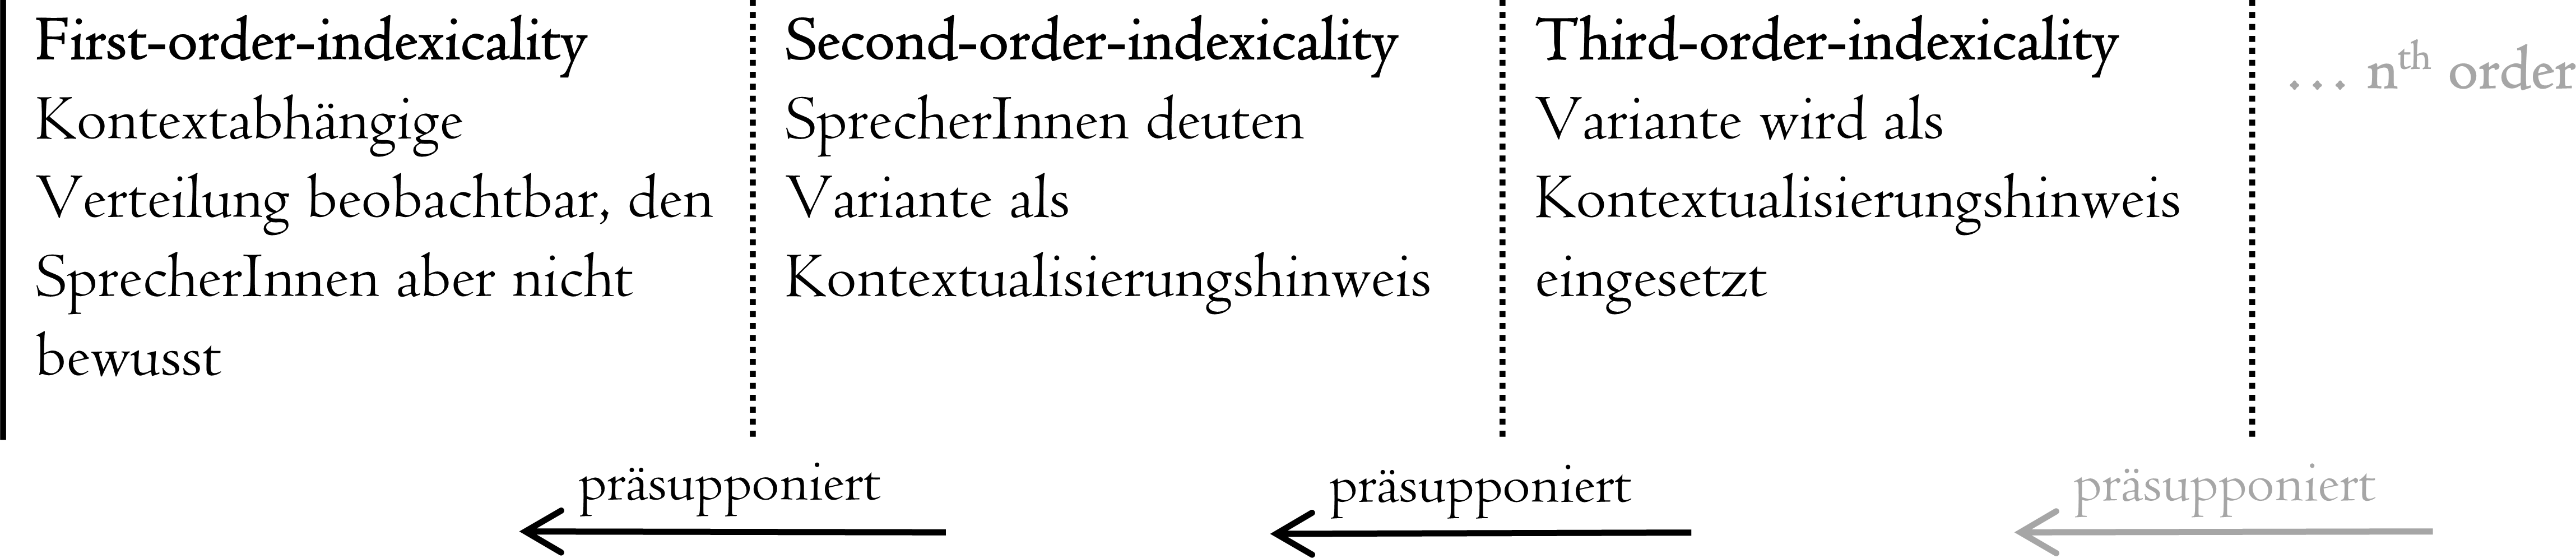
\includegraphics[width=\textwidth]{indexikalischeStufen}
\caption{Indexikalische Stufen nach \citet[]{Silverstein2003}}
\label{pic:Indexikalitaet}
\end{figure}

Wichtig ist, dass die zweite und dritte Ordnung nicht auf einer tatsächlich beobachtbaren Verteilung aufbauen müssen, wie \citet[266]{Spitzmuller2013} betont: \glqq Jede n-te Ordnung präsupponiert die n--1-te Ordnung, was aber nicht bedeutet, dass diese n--1-te Ordnung faktisch wirklich existiert\grqq. 
Studien, die quantitativ untersuchen, welche Gruppe eine Variante h{\"a}ufiger verwendet, k{\"o}nnen daher keinen Aufschluss dar{\"u}ber geben, mit welcher sozialsymbolischen Bedeutung eine Variante aufgeladen ist~\citep[s.][455]{Eckert2008}. 

Da die Verweiskraft in der Interaktion immerzu kreativ genutzt, thematisiert und explizit oder implizit verhandelt wird, ist das System der indexikalischen Ordnungen nach oben offen. 
Sowohl jede Verwendung des Zeichens in einem neuen Kontext als auch die metapragmatische Reflexion tragen zum indexikalischen Gehalt des Zeichens und damit zur weiteren Indexikalisierung bei. 
Das heißt, der Indexikalisierungsprozess ist nie abgeschlossen, sondern die Indexikalität eines Zeichens unterliegt einer ständigen Wandelbarkeit: 

\begin{quote}Variation constitutes a social semiotic system capable of expressing the full range of a community's social concerns. And as these concerns continually change, variables cannot be consensual markers of fixed meanings; on the contrary, their central property must be indexical mutability.~\citep[94]{Eckert2012}
\end{quote}
Auf die dritte indexikalische Stufe können also potenziell beliebig viele weitere Stufen folgen, wie in \autoref{pic:Indexikalitaet} angedeutet~\citep[s.][438]{Woolard2008}.
Sobald eine sprachliche Form einmal von den Sprachbenutzer:innen bemerkt und mit sozialsymbolischer Bedeutung aufgeladen wird, entfaltet sie das Potenzial, mit dem Wissen um die Indexikalität wiederverwendet zu werden und so weitere Bedeutungsfacetten anzunehmen. 
Ein Beispiel, das \citet[13--14]{Eckert.2011} nennt, ist die Realisierung des englischen Phonems \mbox{/θ/} als [t], die in den USA zunächst ein Marker für ethnische Gruppen mit bspw. deutscher oder mexikanischer Herkunft war. 
Auf der nächsten Stufe beinhaltete die Indexikalität dieser Aussprachevariante stereotype Vorstellungen über diese sozialen Gruppen und wurde etwa als Marker für harte Arbeit auf dem Feld gesehen \citep[s.][13]{Eckert.2011}. 
Aufgrund dieser stufenweisen Entwicklung handelt es sich bei indexikalischen Verweisen auf soziale Kategorien oft nicht um einen direkten Verweis der Varianten auf die soziale Kategorie, sondern ein sprachliches Merkmal verweist bspw. indirekt auf eine Gruppe, indem es mit bestimmten Kommunikationspraktiken assoziiert ist, die als typisch für diese Gruppe verstanden werden, oder -- wie im Beispiel von \citet{Eckert.2011} -- andersherum~(\citealp[s.][455]{Eckert2008}; vgl. auch \citealp{Silverstein.1985, Ochs1996}). 

Auf diese Weise kann ein sprachliches Zeichen ein Set an verschiedenen Indexikalitäten entwickeln. 
Um dieser Varianz im Spektrum der indexikalischen Bedeutungen Rechnung zu tragen, entwickelt \citet{Eckert2008} die Idee der indexikalischen Felder, die davon ausgeht, dass eine Variante nicht nur eine Interpretation zulässt, sondern über ein Set von sozialsymbolischen Bedeutungsaspekten verfügt, die je nach Verwendungskontext und beteiligten Akteur:innen aktiviert werden. 
Welcher Aspekt in den Vordergrund rückt, ist dabei sowohl von der Hörerin bzw. dem Leser als auch vom Kotext und dem Inhalt der Äußerung abhängig (\citealp[s.][466]{Eckert2008}; vgl. auch \cites[45]{Gumperz.1992b}[414]{Ochs1996}). 
Als Beispiel nennt \citet[72]{Eckert.2016} das zentralisierte [ɐɪ] aus \citeauthor{Labov1963}s \citeyear{Labov1963} Vineyard-Studie: {\glqq}Once the centralized nucleus indexed an anti-incursion stance on the Vineyard, it was available for reuse, for example, indexing a strong stance on some other issue{\grqq}~\citep[72]{Eckert.2016}.
Je länger eine Variation besteht, desto differenzierter können die indexikalischen Bedeutungsaspekte der Varianten sein \citep[s.][471]{Eckert2008}.

Die Sozialisation der Kommunikationsteilnehmer:innen ist ein wesentlicher Faktor dafür, welche indexikalische Bedeutung ein Zeichen für sie transportiert: 
Als sprachideologische Zuschreibung ist die Indexikalität sprachlicher Varianten sozial stratifiziert \citep[s.][265]{Spitzmuller2013}. 
Die indexikalischen Bedeutungen (bspw. Situation, Zeit, soziale Praktik etc.) werden im Laufe der Sozialisation  mit bestimmten Formen (bspw. Passivformen, Pronomen, bestimmte Fragetypen etc.) verkn{\"u}pft~\citep[s.][410--411]{Ochs1996}.
Auch wenn Kotext, Kontext und Erfahrung aus der eigenen Sprachpraxis das Bedeutungsspektrum der indexikalischen Felder eingrenzen, bleibt die Indexikalität aber immer unscharf, sodass, wie \citet[12--13]{Auer.1995} hervorhebt, zwei Teilnehmer:innen einer Kommunikationssituation den Verweis nie mit den gleichen Worten paraphrasieren würden. 

\begin{sloppypar}
Wie ausdifferenziert die indexikalischen Bedeutungen eines Zeichens sein können, wird an einem weiteren Beispiel deutlich, das \citet[465--466]{Eckert2008} nennt, nämlich den Assoziationen, die die beiden Aussprachevarianten des englischen Suffixes \{-ing\}  hervorrufen. 
Wie Untersuchungen von \citeauthor{CampbellKibler.2007} (\citeyear{CampbellKibler.2005}, \citeyear{CampbellKibler.2007}, \citeyear{CampbellKibler.2008}) zeigen, werden mit den Aussprachevarianten [ɪŋ] und [ɪn] recht unterschiedliche Eigenschaften verbunden. 
\citet{CampbellKibler.2007} lässt in Gruppeninterviews und in einer Umfrage US-amerikanische  Studierende Sprachaufnahmen unterschiedlicher Sprecher:innen bewerten. 
Die natürlichen Aufnahmen werden so manipuliert, dass pro SprecherIn eine Aufnahme mit der Realisierung des Morphems als [ɪŋ] und eine mit der Realisierung als [ɪn] vorliegt. 
Zum einen werden die Varianten als Verweise auf die Herkunft der Sprecher:innen gedeutet: Während [ɪŋ] allgemein der Großstadt zugeordnet wird, gilt [ɪn] als Variante aus Akzenten der Südstaaten \citep[s.][]{CampbellKibler.2007}. 
Zum anderen können die Varianten unterschiedliche Assoziationen mit Sprechertypen hervorrufen: So wird einer der Sprecher, für den die Proband:innen eine großstädtische Herkunft annehmen, signifikant häufiger als homosexuell eingeschätzt, wenn er die Variante [ɪŋ] verwendet \citep[s.][50]{CampbellKibler.2007}. 
[ɪŋ] kann außerdem zu einer höheren Einschätzung der Bildung der Sprecher:innen führen \citep[s.][46--47]{CampbellKibler.2007}. 
[ɪn] hingegen wird unter anderem mit niedriger Bildung und ländlichen Gebieten in Verbindung gebracht. 
Welche Interpretation zum Tragen kommt, ist dabei unter anderem stark von der beurteilenden Person abhängig: 
\end{sloppypar}

\begin{quote} One’s \object{-ing} use is seen by some as more intelligent and by others as annoying, less intelligent, and trying to impress. Another’s \object{-in} guise is seen as compassionate by some and as condescending by others, while a third, when using \object{-in}, is seen by some as annoying and less masculine, while others describe him as a masculine “jock.” \citep[637]{CampbellKibler.2008} \end{quote}
Die Studie \citeauthor{CampbellKibler.2008}s macht deutlich, dass sich die verschiedenen Bedeutungsmöglichkeiten einer Variante durchaus widersprechen können \citep[vgl. auch][93--94]{Jaffe.2016}. 
Offenbar ist für die Interpretation unter anderem entscheidend, ob (aufgrund von Kontext und Kotext) angenommen wird, dass eine Variante Teil des \glqq natürlichen\grqq{} Sprachgebrauchs einer Person ist, oder ob davon ausgegangen wird, dass die Variante bewusst eingesetzt wird, um einen bestimmten Effekt zu erzielen \citep[s.][640]{CampbellKibler.2008}. 
Das Aufzeigen differenzierter indexikalischer Felder macht auch deutlich, dass die häufig vorgenommene Unterteilung in eine {Pres\-tige\-variante} und eine stigmatisierte Variante meistens stark vereinfachend ist \citep[s.][226]{Eckert2004}. 

Einzelne oder mehrere Indexikalitäten können Zeichen mit anderen Zeichen gemeinsam haben, sodass diese Zeichen über ihre indexikalischen Bedeutungen untereinander verbunden sind. 
So kann ein Set von über die Indexikalität vernetzten Sprachzeichen ein sprachliches Register bilden. 
Register lassen sich im linguistisch-anthropologischen Verständnis als ein Repertoire von Zeichen verstehen, das über Sprachideologien mit bestimmten kommunikativen Praktiken und deren Akteur:innen verknüpft ist (\cites[s.][216]{Agha.1999}[38]{Agha2005}). 
Auch sie werden also im metapragmatischen Diskurs konstruiert \citep[s.][46]{Agha2005}. 
Der Prozess dieser sprachideologischen Konstruktion von Registern wird als Registrierung oder \textit{Enregisterment} bezeichnet (s. \cites[231]{Agha2003}[268]{Spitzmuller2013}{Anderwald.2017}). 
Dabei werden Varianten durch ihren Gebrauch sowie durch metapragmatische Kommentare bspw. einer Fachsprache, einer Textsorte etc. zugeordnet \citep[s.][218]{Agha.1999}. 
Die Herausbildung einer Standardsprache etwa ist als Registrierungsprozess zu fassen, an dem verschiedene soziale Akteure, wie etwa Schulen, die Medien usw. beteiligt sind (\cites[s.][64]{Woolard1994}{Auer.2013}). 
Auch das Entstehen von W{\"o}rterb{\"u}chern, Grammatiken und Sprachpflegevereinen tr{\"a}gt zur Registrierung einer Standardsprache bei~\citep[s.][164]{Gal.2006b}.

\begin{sloppypar}
Eine klare Trennung in Register als situationsspezifische Sprachgebr{\"a}uche und Variet{\"a}ten, die bestimmten Personen oder Personengruppen zugeschrieben werden, ist aufgrund der Menge an interagierenden Faktoren und der engen Verwobenheit der Indexikalit{\"a}ten kaum m{\"o}glich \citep[s.][120--121]{Eckert2005}. Vielmehr sind über den Registerbegriff verschiedene Kriterien miteinander verbunden: {\glqq}In all cases, a cultural model associates speaker types, their typified features, activities, practices, and values with a way of speaking: a register{\grqq}~\citep[117]{Gal.2016}. 
Dabei soll die Registrierung einer Form hier nicht mit ihrer Indexikalisierung gleichgesetzt werden:
Bspw. können die verschiedenen Formen, die dem Repertoire der Standardsprache zugeordnet sind, über ganz unterschiedliche Indexikalitäten verfügen \citep[s.][122]{Eckert2005}. 
Möglicherweise verweisen einige Formen des Repertoires auf Bildung, während andere als literatursprachlich oder altmodisch gelten.
\end{sloppypar}

Aus den Konzepten der Indexikalität und der Registrierung ergibt sich, dass es sich bei sprachlichen Varianten oder verschiedenen Stilen keineswegs schlicht um verschiedene Arten handelt, das Gleiche auszudrücken (\cites[s.][28]{Auer.1989}[88]{Coupland.2007}). 
\citet[96]{Eckert2012} konstatiert: \glqq style is at its foundation ideological, and the stylistic form of propositions is very much a part of their meaning\grqq.
Die indexikalische Bedeutung eines Zeichens ist dabei nicht statisch, sondern wird über den Diskurs vermittelt und ständig weiterentwickelt. 
\subsubsection{Ausblendung, fraktale Rekursivität und Ikonisierung}
\label{sec:Prozesse}
% Andersherum kann es auch vorkommen, dass vorhandene soziologische Unterschiede und der Wunsch nach Differenzierung dazu f{\"u}hren, dass sprachliche Variation verst{\"a}rkt wird~\citep[s.][39]{Irvine2000}.
\citeauthor{Irvine2000} (\citeyear{Irvine2000}, \citealp[s. auch][]{Gal.1995} \citeyear[und][]{Gal.2019}) machen drei wesentliche Prozesse aus, die bei sprachideologischen Konzeptualisierungen eine Rolle spielen:~Ausblendung, fraktale Rekursivit{\"a}t und Ikonisierung. 
Sie können die Indexikalität und den Registrierungsprozess stützen und stellen wichtige Faktoren bei der Wahrnehmung sprachlicher Variation dar.
Damit bilden die drei von \citet{Irvine2000} beschriebenen Prozesse gewissermaßen die diskursiven Dynamiken, unter denen Indexikalisierungs- und Registrierungsprozesse entstehen. 

%Ausblendung
\begin{sloppypar}
Der Prozess der Ausblendung (\textit{erasure}) f{\"u}hrt nicht prim{\"a}r dazu, dass ein sprachliches Element oder seine Eigenschaften tats{\"a}chlich ausgel{\"o}scht werden; vielmehr werden sie im Diskurs nicht wahrgenommen oder mit Behelfserkl{\"a}rungen ins Bild eingepasst \citep[s.][38]{Irvine2000}.   
Dies zeigt sich bspw. in einer Untersuchung von \citet{Auer.2017} zum Gebrauch verschiedener Dialektmerkmale am Oberrhein. 
Für dieses Gebiet wurde in der Dialektologie lange angenommen, dass die Dialektgrenze quer zur deutsch-französischen Staatsgrenze verläuft.
Isoglossen, die sich entlang der Staatsgrenze erstrecken und diesem Bild damit widersprechen, wurden ausgeblendet \citep[s.][29]{Auer.2017}. 
Diese Vernachlässigung bestimmter {Va\-rian\-ten\-ver\-tei\-lungen} war vor allem politisch motiviert: \citet{Auer.2017} zitieren insbesondere \citet{Maurer.1942} und merken an: 
\begin{quote} Es bedarf kaum der Erwähnung, dass diese Einschätzung in einem 1942 erschienenen Buch, das \glqq unseren Kameraden an der Front und bei der Wehrmacht\grqq{} gewidmet war, auch ein politisches Statement war. Maurers Darstellung der \glqq Rheinstaffeln\grqq{} [...] ist nicht zuletzt durch die geschickte Wahl der Merkmale bedingt.~\citep[29]{Auer.2017}\end{quote}
Im Metasprachdiskurs {\"u}ber die Sekund{\"a}rpr{\"a}positionen l{\"a}sst sich die ideologische Ausblendung der urspr{\"u}nglichen Dativpr{\"a}positionen und ihres Wandels zum Genitiv beobachten: Sprachbenutzer:innen gehen oft davon aus, dass die Genitivrektion grundsätzlich die ältere Form darstellt \citep[s.][46]{Szczepaniak2014}. 
Teilweise gehen infolge der ideologischen Ausblendung sprachliche Elemente aber auch tatsächlich aus einer Variet{\"a}t oder Sprache verloren \citep[s.][38--39]{Irvine2000}.
\end{sloppypar}

%fraktale Rekursivität
Mit fraktaler Rekursivit{\"a}t beziehen sich \citet[38]{Irvine2000} auf die Beobachtung, dass Unterscheidungen, die auf einer Ebene getroffen werden, auf eine andere Ebene projiziert werden. 
Bspw. wird von vielen Sprachkritiker:innen zwischen \glqq gutem\grqq{} und \glqq schlechtem\grqq{} Deutsch unterschieden. 
Zu letzterem werden häufig Anglizismen gezählt. 
Innerhalb der Gruppe der Anglizismen wird allerdings wieder unterschieden zwischen solchen, die eine Lücke im Wortschatz füllen, und daher als notwendig erachtet werden (etwa \object{Internet}) und solchen, die (scheinbar) eine Entsprechung im Deutschen haben\footnote{Meistens handelt es sich hier lediglich um partielle Synonyme oder Anglizismus und Erbwort entsprechen sich zwar auf der denotativen Ebene, verfügen aber über unterschiedliche Indexikalitäten und werden daher von unterschiedlichen Personengruppen/in unterschiedlichen Kontexten gebraucht \citep[s. hierzu][]{Spitzmuller.2007}.}, und daher als überflüssig und unerwünscht betrachtet werden (etwa \object{Party}). 
Zu einer Opposition werden also Unterkategorien gebildet, die sich wieder gegen{\"u}berstehen. 
Im Falle der Kasusschwankungen bei Sekund{\"a}rpr{\"a}positionen könnte sich die Rekursivit{\"a}t wie folgt zeigen:~Die Sprachbenutzer:innen differenzieren zwischen verschiedenen sozialen Gruppen, bspw. Akademiker:innen und Nichtakademiker:innen. Diese Unterscheidung wird auf Unterschiede zwischen Kommunikationspraktiken und Registern projiziert, etwa dienstliche formelle E-Mails im Gegensatz zu informellen mündlichen Gesprächen. 
Diesen unterschiedenen Registern werden die wahrgenommenen Varianten der Kasusrektion, Genitiv- und Dativrektion zugeordnet~(s. \autoref{sec:IndexikalitaetRektionskasus}).

%Ikonisierung
Mit Ikonisierung ist gemeint, dass ein sprachliches Merkmal als so charakteristisch für eine soziale Gruppe oder einen Kommunikationskontext angesehen wird, dass es geradezu als Stellvertreter für diese bzw. diesen angesehen wird. 
In der Wahrnehmung der Sprecher:innen entsteht ein Abbildverh{\"a}ltnis zwischen dem sprachlichen Merkmal und einem au{\ss}ersprachlichen Merkmal~\citep[s.][37]{Irvine2000}. 
Dadurch rücken Bezeichnetes und Bezeichnung näher zusammen, sodass sich die Zeichenhaftigkeit ein Stück weit auflöst und die Verbindung naturalisiert wird. 
Bspw. wird Sprache als Abbild für Nationalität gesehen, eine Ideologie, die auf Herder zurückgeht \citep[s.][60]{Irvine2000}. 
Hier wird ein Ähnlichkeitsverhältnis (bzw. ein Gleichheitsverhältnis) zwischen der Ausdehnung einer Sprache oder Varietät und der Ausdehnung eines Volkes angenommen. 
Auf Grundlage dieser Sprachideologie wurden während der Kolonialzeit Gebiete anhand von (vermeintlich eindeutigen) Sprachgrenzen eingeteilt, wie \citet[48--49]{Irvine2000} am Beispiel Westafrikas zeigen. 
Als ikonisch kann auch der Gebrauch von Majuskeln bis zur vollständigen Durchsetzung der heutigen Konventionen zur Großschreibung im Deutschen angesehen werden:
Im Frühneuhochdeutschen wurden insbesondere Namen von Personen, denen Ehrerbietung und Respekt entgegengebracht wurde, mit Majuskeln versehen (\cites[s.][]{Ducker.2020b}[73]{Bergmann.1999}). 
Noch verbreiteter war die Großschreibung von Wörtern wie \object{Gott} oder \object{Herr}. 
Ein weiteres Beispiel, das sich als Ikonisierung einordnen lässt, ist, dass Grammatikfehler von vielen als Zeichen mangelhafter Denkfähigkeit angesehen werden \citep[s.][11]{Eisenberg1990b}. 

Da ikonische Zeichen auf einem {\"A}hnlichkeitsverh{\"a}ltnis von Form und Inhalt beruhen, sind diese hier noch enger verkn{\"u}pft als bei indexikalischen Zeichen. 
Die Ikonisierung kann daher als ein weiterer Schritt in der Konventionalisierung einer indexikalischen Bedeutung verstanden werden \citep[s.][86]{Jaffe.2016}. 
Dass es sich um eine ideologisch vermittelte Verbindung handelt, wird dann nicht mehr wahrgenommen: \begin{quote} Viewed in this light, the process of indexicalization itself can be the target of processes of {“}erasure,{”} to use another of Gal and Irvine's terms. That is, iconization can be understood as erasing the situated, contingent, and political nature of indexical links between language/semiotic practice and aspects of the social world.~\citep[87]{Jaffe.2016}\end{quote}
Der Prozess, in dem ein indexikalisches Zeichen zum Ikon wird, wird von \citet[123]{Gal.2016} als Ikonisierung oder auch Rhematisierung bezeichnet.
Ob ein Zeichen als Index oder als Ikon interpretiert wird, hängt häufig von der interpretierenden Person und ihrer Teilhabe an sprachideologischen Diskursen ab~\citep[s.][122]{Gal.2016}. 

Auch die Prozesse der fraktalen Rekursivität und der Ausblendung stehen in engem Zusammenhang mit der Indexikalisierung sprachlicher Zeichen. 
So können bspw. soziale Kategorien wie die Generationen einer Gesellschaft und die ihnen zugeschriebenen Eigenschaften als Vorlage für die Indexikalitäten dienen, die sprachlichen Varianten zugeschrieben werden. 
Die Unterschiede, die auf der Ebene gesellschaftlicher Gruppen angenommen werden, werden dann auf sprachliche Unterschiede projiziert. 
Die Ausblendung bestimmter Merkmale kann die Indexikalisierung stützen, indem Widersprüche verschleiert werden. 
So werden bspw. standardkonforme Merkmale in stigmatisierten Registern wie der Jugendsprache oft nicht beachtet \citep[s.][143]{Hundt.2017b}. 
Diese Beispiele machen deutlich, wie die von \citet{Irvine2000} beschriebenen sprachideologischen Prozesse an der Aushandlung der indexikalischen Bedeutung sprachlicher Merkmale beteiligt sind. 
\subsubsection{Sprachideologische Positionierung}
\label{sec:Positionierung}
Aufgrund der sprachideologischen Verbindung von sprachlichen Formen mit sozialen Bedeutungen ist Sprache nie ausschließlich ein Informationsmedium, sondern immer auch ein Ausdruck der Werthaltungen von Sprachbenutzer:innen (s.~\cites[491]{HessLuttich2005}[95]{Bell.2007}[195]{Spitzmuller.2007}). 
\citet[40]{Agha2005} etwa hebt hervor, dass sich in der Wahl eines Stils oder bestimmter Varianten erkennen lässt, wie die Sprecherin zu etwas steht. 
So werden sprachliche Mittel etwa eingesetzt, um sich von anderen abzugrenzen oder Zugehörigkeit zu einer Gruppe auszudrücken \citep[s.][17]{Silverstein.1976}.
Dies wird mithilfe des Konzeptes der Positionierung oder des \textit{stancetaking} beschrieben (\cites[s.][]{DuBois.2007}{Jaffe.2016}{Spitzmuller.2017b}). 

Die Positionierung besteht zunächst aus der Beurteilung oder Bewertung eines beliebigen Objekts:
\glqq The act of taking a stance necessarily invokes an evaluation at one level or another, whether by assertion or inference\grqq{} \citep[141]{DuBois.2007}.
Als sozialer Akt lässt sich Positionierung fassen, weil neben dem Bewertenden und dem Objekt der Bewertung (\textit{object of stance} bei \citeauthor{DuBois.2007}) eine dritte Seite relevant ist:
Indem eine Akteurin ein Objekt bewertet, positioniert sie sich zu diesem ebenso wie zu anderen Akteur:innen, die entweder eine ähnliche oder eine abweichende Position gegenüber diesem Objekt haben.\footnote{Welche Positionen eingenommen werden können, ist nicht beliebig: Die (veränderbare) {Dis\-kurs\-struk\-tur} eröffnet bestimmte Möglichkeiten der Positionierung, während andere nicht gegeben sind (\cites[s.][82]{Foucault.1981}[4]{Spitzmuller.2017b}).}
\citet[163]{DuBois.2007} bringt dies auf die Formel {\glqq}I evaluate something, and thereby position myself, and thereby align with you{\grqq}.

Das Modell von \citet{DuBois.2007} erweitert \citet[273]{Spitzmuller2013} zu einem Modell der sprachideologischen Positionierung (s. \autoref{pic:Briefumschlag}). 
Darin ist berücksichtigt, dass sich die Kritik an sprachlichen Formen nicht trennen lässt von der Kritik an damit indexikalisch zusammenhängenden außersprachlichen Größen (\citealp[s.][257]{Spitzmuller.2005}; vgl. auch \citealp[1]{Gal.2019}). \citet[272]{Spitzmuller2013} nennt den Personentypus und den Verhaltenstypus als die zentralen sozialen Kategorien, die über Indexikalisierungs- und Registrierungsprozesse an sprachliche Formen angebunden werden und über diese untereinander verknüpft sind. 
Indem eine Sprachbenutzerin bspw. eine sprachliche Form wie den Apostroph in \object{frische Pizza's} bewertet, positioniert sie sich immer auch zu den sozialen Werten und Kategorien, die mit dieser Form assoziiert sind.
Im Modell ist dies durch die unterbrochenen Linien oberhalb und unterhalb der Dreiecke dargestellt. 
Aber nicht nur explizite metapragmatische Äußerungen beinhalten eine Positionierung zu einem bestimmten Sprachgebrauch. 
Auch indem ein Sprachbenutzer eine sprachliche Form selbst auf eine bestimmte Art und Weise verwendet, positioniert er sich dazu \citep[s.][270]{Spitzmuller2013}. 
Gleichzeitig evoziert und bewertet er dadurch die mit der Form indexikalisch verbundenen Kategorien. 
Bspw. kann er sich durch die Verwendung eines Wortes in Anführungszeichen von dem Gebrauch dieses Wortes und den damit assoziierten Personen- und Verhaltenstypen distanzieren.\footnote{S. dazu \citet[]{Klockow.1980}, der verschiedene einen Vorbehalt ausdrückende Verwendungen von Anführungszeichen unterscheidet \citep[vgl. auch][]{Bredel.2011}.}
Andererseits kann durch einen unironischen, nicht distanzierenden Gebrauch Zugehörigkeit oder Zustimmung zu den durch eine Form indizierten Kategorien ausgedrückt werden.

\begin{figure}
\centering
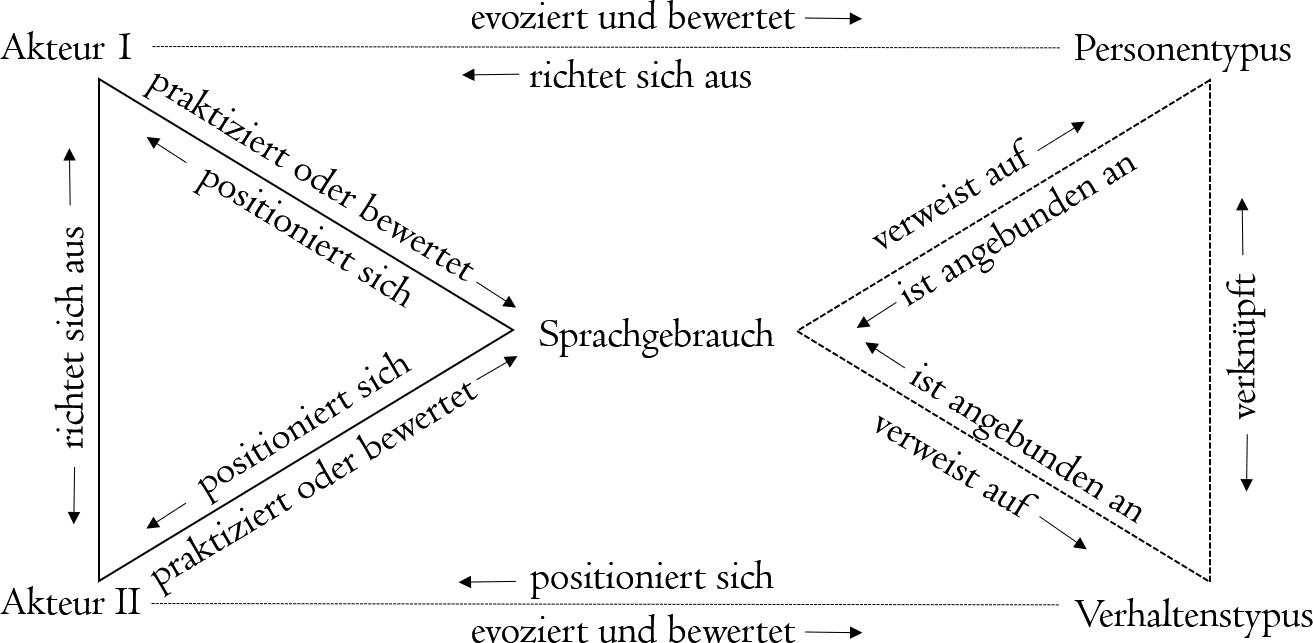
\includegraphics[width=\textwidth]{Briefumschlag}
\caption{Modell der sprachideologischen Positionierung von \citet[273]{Spitzmuller2013}, aktualisiert durch \citeauthor{Spitzmuller2013} (persönliches Gespräch)}
\label{pic:Briefumschlag}
\end{figure}

Wichtig ist jedoch, dass eine Position nicht als etwas anzusehen ist, das im Bewusstsein von Personen verankert ist, sondern als eine Größe, die erst durch eine konkrete Äußerung entsteht~\citep[s.][369--370]{Deppermann.2015}. 
Welche Position jemand relevant macht, kann daher je nach Situation variieren: 
\begin{quote}Positions are locally occasioned and designed, they are temporally and situationally flexible, and they are multifaceted – that is, different facets of identity are relevant in different discursive contexts. \citep[370]{Deppermann.2015}\end{quote}
So lassen sich auch die Rollen von Laie und Expertin als Positionen auffassen, die in einer konkreten Situation eingenommen werden, wie in \autoref{sec:Laienlinguistik} beschrieben. Die Positionierung als Expertin kann dabei etwa durch die Verwendung von Fachbegriffen vorgenommen werden, die als Laie bspw. durch den Ausdruck der emotionalen Bewertung eines Phänomens. 

Mit jeder Verwendung oder metapragmatischen Thematisierung einer indexikalisch aufgeladenen Form sagt eine Person A auch etwas über ihre Ausrichtung gegenüber anderen aus. 
Erstens gegenüber konkreten anderen an der Interaktion beteiligten Personen, etwa wenn eine Person B auf ironische Weise das Wort \object{Personenvereinzelungsanlage} verwendet und Person A darüber lacht. 
Zweitens richtet sie sich dadurch gegenüber einer stereotypen Vorstellung von Personen aus, mit deren Sprachgebrauch dieses Wort assoziiert ist \citep[s.][119]{Gal.2016}. 
Sie positioniert sich also zu einem abstrakten Personentypus, der \citeauthor{Bachtin.1990}s (\citeyear{Bachtin.1990}) Konzept der \textit{Persona} entspricht. 
\textit{Personae} können indexikalisch mit sprachlichen Repertoires verbunden sein, sodass auf sie verwiesen werden kann, indem ein Element dieses Repertoires genutzt wird \citep[s.][118]{Gal.2016}. \citet[39]
{Agha2005} spricht daher von \glqq figures performed through speech\grqq{} und verknüpft die Positionierungstheorie so mit einem zweiten Konzept \citeauthor{Bachtin.1990}s (\citeyear{Bachtin.1990}), dem \textit{voicing}. Damit ist gemeint, dass durch die Verwendung registrierter Formen stereotype Personentypen dargestellt werden können: \glqq every register has a social range, a range of figures performable through its use\grqq{} \citep[39]{Agha2005}. 

Das \textit{voicing}\footnote{In der Soziolinguistik ist oft auch von Stilisierung die Rede \citep[s. bspw.][]{Coupland.2007}.} ist insbesondere durch sprachliche Zeichen dritter oder drei +$n$ter indexikalischer Ordnung(en) möglich. 
Das oben herangezogene Beispiel der Verwendung von \object{ich} mit Aussprache des [\c{c}] als [ʃ] etwa wäre ein Fall von \textit{voicing}, mit dem sich eine Sprecherin oder ein Sprecher gegenüber durch diese Form indizierten Gruppen positionieren kann. 
Dass Indexikalität und Register dynamische Größen sind, die durch die Positionierungspraxis selbst gefestigt, verändert oder infrage gestellt werden können, ist im Positionierungsmodell durch die unterbrochenen Linien dargestellt \citep[s.][273]{Spitzmuller2013}. 
Eine Positionierung zu einer sprachlichen Form ist also nur vor dem Hintergrund der indexikalischen Bedeutung dieser Form zu verstehen und trägt gleichzeitig zur Indexikalisierung der Form bei. 
Ebenso kann sie Anzeichen und Katalysator für Ausblendung, fraktale Rekursivität und Ikonisierung sein. 

\subsection{Spracheinstellungen und Sprachideologien: Theoretische und methodologische Zusammenführung}
\label{sec:Integrationsversuch}
\begin{sloppypar}
Häufig wird von Sprachideologieforschung und Spracheinstellungsforschung als verschiedenen Sichtweisen auf ein und dasselbe Phänomen gesprochen, da beide metapragmatische Bewertungen von Sprache zum Gegenstand haben. 
Bei näherer Betrachtung zeigt sich jedoch, dass die Ansätze unterschiedliche Schwerpunkte haben. 
Während die Sprachideologieforschung an Zusammenhängen von Sprache und Gesellschaft interessiert ist, fokussiert die Spracheinstellungsforschung auf die kognitive Ebene und die Bewertung sprachlicher Phänomene durch einzelne Personen. 
Ziel der Spracheinstellungsforschung ist es dabei in erster Linie, etwas über Varietäten zu erfahren; 
Ziel der Sprachideologieforschung hingegen ist es, etwas über das gesellschaftliche Zusammenleben zu erfahren, sie hat also ein stärker kulturanthropologisch ausgerichtetes Interesse. 
Die Zusammenhänge zwischen der gesellschaftlichen und der individuellen Ebene sollen im \autoref{sec:GesellschaftundIndividuum} erläutert werden. 
Die Kritik an der sozialpsychologisch geprägten Spracheinstellungsforschung lautet oft, ihre Theorie sei unterkomplex und positivistisch (\citealp[s. etwa][141]{Agheyisi.1970}; s. hierzu auch \citealp{Soukup.2014}). 
Inwiefern sich beide Ansätze dennoch unter einem konstruktivistischen Paradigma vereinen lassen, wird in \autoref{sec:Konstruktivismus} diskutiert. 
Schließlich werden aus den Überlegungen methodologische Implikationen für die Untersuchung metapragmatischer Äußerungen abgeleitet (\autoref{sec:Methodologie}). 
\end{sloppypar}
\subsubsection{Metapragmatik zwischen Gesellschaft und Individuum}
\label{sec:GesellschaftundIndividuum}
%Was ist eigentlich mit diesem Gegensatz, dass die Spracheinstellungsforschung verallgemeinern will und die Sprachideologieforschung lokale Praxen untersucht? Muss das noch irgendwo rein? 
Die Begriffe Spracheinstellungen und Sprachideologien können mit \citet[22]{Konig.2014} unterschiedlichen konzeptuellen Ebenen zugeordnet werden. 
Während es bei der Untersuchung von Sprachideologien um Vorstellungen verschiedener sozialer Gruppen geht, stehen bei der Beschäftigung mit Spracheinstellungen die Vorstellungen einzelner Personen im Vordergrund \citep[s.][24]{Konig.2014}.
Zudem werden unter Sprachideologien h{\"a}ufig nicht nur metapragmatische Annahmen zu einzelnen Ph{\"a}nomenen verstanden, sondern Systeme von Vorstellungen {\"u}ber Sprache (\citealp[24]{Konig.2014} verweist hier auf \citealp[970]{Gal.1995} und \citealp[35]{Irvine2000}).

Eine Spracheinstellungsforschung, die aus metapragmatischen Äußerungen kognitive Strukturen ableiten will, verfolgt ein grundsätzlich anderes Ziel als die Sprachideologieforschung, die in Metapragmatik in erster Linie soziale Handlungen sieht.
Vertreter:innen beider Forschungsrichtungen betonen aber den engen Bezug zwischen Sprachideologien und Spracheinstellungen. \citeauthor{Woolard1994} (\citeyear[61--62]{Woolard1994}) sehen in Spracheinstellungen einzelner Sprecher:innen die Spiegelung der in einer Gesellschaft vorhandenen Sprachideologien \citep[vgl. auch][161--162]{Milroy2004}. 
Ähnlich geht \citet[xxiv]{Preston.1999b} davon aus, dass Spracheinstellungen von \textit{folk beliefs} beeinflusst werden, bspw. von Vorstellungen {\"u}ber den Status von Variet{\"a}ten oder über Eigenschaften von deren Sprecher:innen \citep[ähnlich auch][34]{Garrett.2012}.  
Auf solche in der Gesellschaft geteilten, nicht hinterfragten Sprachideologien berufen sich Sprecher:innen bei metapragmatischen Äußerungen (\cites[s.][1]{Gunthner.2012}[vgl. auch][205]{Konig2015}). 
Was die Frage nach der Entwicklung von Spracheinstellungen angeht, h{\"a}lt \citet[732]{Neuland.1993} fest, dass bisherige Untersuchungen hierzu nahelegten, dass Kinder und Jugendliche sich in ihren Spracheinstellungen nach und nach den dominanten Bewertungsmustern der Gesellschaft ann{\"a}herten. 
Auch \citet[399]{Lasagabaster.2005} geht davon aus, dass Sprecher:innen ihre Einstellungen an die in ihrer Gruppe geteilten Ideologien angleichen. 
Dies macht deutlich, wie individuelle Spracheinstellungen von gesellschaftlich geprägten Sprachideologien durchformt werden~\citep[s.][732]{Neuland.1993}. 
Dabei ist davon auszugehen, dass Ideologien alle drei Komponenten speisen, die eine Spracheinstellung konstituieren. 
So besteht etwa die kognitive Komponente im Wesentlichen aus dem Wissen um die Indexikalitäten, die einer Form gesellschaftlich zugeschrieben werden. 
Ebenso lassen sich mit dem Konzept der Indexikalität aber auch die Verhaltensebene (wann verwende ich eine Form/welche Annahmen habe ich darüber, wann ich eine Form verwende?) und die affektive Komponente (mit welchen Emotionen ist eine Form besetzt?) beschreiben. 
Der Bezug der eigenen Einstellung zu gesellschaftlich vermittelten Ideologien ist den Angehörigen einer Sprachgemeinschaft allerdings meist nicht bewusst \citep[s.][133]{Milroy.2007}.

\begin{sloppypar}
Da Sprachideologien von der Gesellschaft reproduziert und dadurch in gewisser Weise normalisiert werden, erscheinen sie als selbstverst{\"a}ndlich~\citep[s.][10]{Blommaert.1999} und können auch Spracheinstellungen wie selbstverst{\"a}ndlich erscheinen lassen \citep[s.][123]{Androutsopoulos.2007}.
Ein Beispiel daf{\"u}r ist der von \citet[134]{Milroy.2007} in Standardsprachkulturen beobachtete {\glqq}belief in correctness{\grqq}:~Auf der Standardsprachideologie, also der Vorstellung einer einheitlichen Leitvariet{\"a}t, fu{\ss}t die Auffassung, manche Varianten seien korrekt und andere inkorrekt. 
Diese Ideologie {\"a}u{\ss}ert sich in einer ablehnenden Einstellung gegenüber manchen Formen, die als {\glqq}falsch{\grqq} eingeordnet und der Folge davon sanktioniert werden~\citep[134]{Milroy.2007}.
\end{sloppypar}

\begin{sloppypar}
Es wird also deutlich, wie eng Spracheinstellungen mit Sprachideologien zusammenhängen: Sprachideologien bestimmen zu einem Teil, wie Sprecher:innen sprachliche Merkmale konzeptualisieren und wie sie sie bewerten \citep[s.][206]{Maitz2015}. 
\citet[8]{Garrett.2012} sieht Sprachideologien daher als Rechtfertigungen und Unterst{\"u}tzungen f{\"u}r Spracheinstellungen. 
Spracheinstellungsäußerungen präsupponieren häufig Sprachideologien, indem sie auf \glqq vorgeformte, soziale Kategorisierungen\grqq{} \citep[][213]{Tophinke.2006} verweisen.
Auf diese Weise lassen Äußerungen über Spracheinstellungen auf zugrundeliegende Sprachideologien schließen \citep[s.][35]{Garrett.2012}.
Sprachideologien und Spracheinstellungen können somit als interdependent modelliert werden:
Vor der Folie etablierter Sprachideologien wie etwa der Standardsprachideologie (s. \autoref{sec:MetapragmatikVariationWandel}) werden Spracheinstellungen geäußert. 
Diese stellen nicht nur eine Positionierung zu einem sprachlichen Phänomen dar, etwa zum Kiezdeutschen, sondern auch zu den damit verbundenen Ideologien. 
So kann bspw. eine negative Einstellungsäußerung zum Kiezdeutschen die Ideologie, der Standard stünde über anderen Varietäten, festigen. 
Trotz dieser engen gegenseitigen Abhängigkeit von Spracheinstellungen und Sprachideologien ist davon auszugehen, dass weder Sprachideologien allein aus Spracheinstellungen entstehen noch Spracheinstellungen sich allein aus Ideologien speisen. 
Bspw. ist es möglich, dass jemand eine positive Einstellung gegenüber einem bestimmten Lexem oder einem bestimmten Dialekt hat, weil er es oder ihn mit dem Sprachgebrauch eines ihm nahestehenden Menschen verbindet. 
Es ist jedoch davon auszugehen, dass Spracheinstellungen nicht ohne grundlegende Konzeptualisierungen von Sprache und damit ohne Rückgriff auf Sprachideologien entwickelt und ausgedrückt werden können:
\end{sloppypar}

\begin{quote}Jeder Standpunktbezug kommuniziert, da er die Bewertung eines {\frq}Objekts{\flq} einschlie{\ss}t und somit Werte und Einstellungen zum Ausdruck bringt, Ideologien.~\citep[270]{Spitzmuller2013}\end{quote}
Für die Entstehung von Sprachideologien auf der anderen Seite sind Spracheinstellungsäußerungen allein nicht ausreichend, sie müssen an bestehende Ideologien anknüpfen und gesellschaftlich geteilt werden. 
In der vorliegenden Studie % Änderung Anfang
soll nicht auf Spracheinstellungen als kognitive Größe, sondern auf Spracheinstellungsäußerungen als konkrete Wertungen fokussiert werden, % Änderung Ende 
die vor dem Hintergrund der in einer Gesellschaft diskursiv ausgehandelten Sprachideologien entstehen und auf diese zurückwirken. 
\subsubsection{Konstruktivistischer Ansatz}
\label{sec:Konstruktivismus}
Wie die Ausführungen zu Spracheinstellungsforschung und Sprachideologieforschung gezeigt haben, unterscheiden sich beide Traditionen zum Teil stark in ihren theoretischen Grundannahmen. 
Der Spracheinstellungsforschung ging es lange Zeit vor allem um die Bewertung selbst und ihre kognitive Manifestation.
So spricht etwa \citeauthor{Neuland.1993} von sprachlichen Formen als Identifikationsmerkmalen, die 
\begin{quote} Attributionen von Merkmalen des Alters und Geschlechts, von nationaler und regionaler Herkunft und Sozialstatus sowie von Pers{\"o}nlichkeitseigenschaften ausl{\"o}sen k{\"o}nnen. \citep[730]{Neuland.1993} \end{quote}
Wie diese Verkn{\"u}pfungen zustande kommen, ist allerdings in vielen Spracheinstellungsstudien nicht Teil der Fragestellung, wie \citet[730]{Neuland.1993} selbst anmerkt.\footnote{Die meisten Spracheinstellungsstudien entsprechen daher dem Ansatz der ersten soziolinguistischen Welle, während die Sprachideologieforschung der dritten Welle verpflichtet ist \citep[s.][]{Eckert2012}.}  
Dennoch beobachtet \citet[120]{Garrett.2007} eine Annäherung an die Sprachideologieforschung, da die Spracheinstellungsforschung zunehmend auch daran interessiert sei, soziale Zuschreibungen kritisch zu hinterfragen.

Das Konzept der Sprachideologien ist hingegen grundsätzlich ein {konstruk\-ti\-vis\-tisches}. 
So stellt \citet[25]{Konig.2014} fest, dass die Sprachideologieforschung verstärkt an der Frage nach semiotischen Prozessen bei der Indexikalisierung und Registrierung sprachlicher Zeichen (\autoref{sec:Indexikalitaet}) interessiert ist. 
In der Sprachideologieforschung werden aber nicht nur die Verknüpfungen von sprachlichen und gesellschaftlichen Kategorien als ideologische Konstrukte angesehen, sondern auch die Kategorien selbst: 
\begin{quote}The “language reflects society” account implies that social structures somehow exist before language, which simply “reflects” or “expresses” the more fundamental categories of the social. Arguably however we need a far more complex model that treats language as \textit{part }of the social, interacting with other modes of behaviour and just as important as any of them. \citep[81--82]{Cameron.1990}
\end{quote}
Auch \citet{Irvine.2005} betont, dass sowohl sprachliche als auch soziale Kategorien nicht als gegeben angenommen werden dürfen: 
\begin{quote}By foregrounding ideology I emphasize the need to investigate ideas about language and speakers independently of empirical distributions, and the need to recognize that {\glq}attitudes{\grq} include participants' basic understandings of what the sociolinguistic system consists of, not just emotional dispositions. Moreover, the categories and behaviors toward which one has these attitudes cannot be assumed to have been established independently of anyone's perception of them.~\citep[24]{Irvine.2005}\end{quote}
Dieser zusätzliche Analyseschritt kann und sollte auch für die Spracheinstellungsforschung nutzbar gemacht werden.  
Auch neuere Spracheinstellungsstudien fordern daher stärker konstruktivistisch ausgerichtete Herangehensweisen (\cites[s.][207]{Tophinke.2006}[195]{Liebscher.2009}[61--62]{Cuonz.2014}).
So machen bspw. \citet[213]{Tophinke.2006} deutlich, dass man zwar davon ausgehen könne, dass Personen einen bestimmten Beruf haben usw., es allerdings von den {Kom\-mu\-ni\-kations\-teil\-neh\-merIn\-nen} abhänge, ob dies im Kontext einer Spracheinstellungsäußerung relevant werde. 

In der diskursiven Sozialpsychologie wird daher ein konstruktivistischer Ansatz verfolgt, der nicht an Einstellungen als mentalen Konstrukten interessiert ist, sondern danach fragt, welche konkreten Bewertungspraktiken sich beobachten lassen und wie Bewertungen von Sprache in der Interaktion genutzt werden (\citealp[s.][234]{Potter.1998}; s. auch die Beiträge in \citealp{Cuonz.2014b}). 
Damit geht eine Verschiebung des Forschungsinteresses einher: 
\begin{quote}Im Sinne des Konstruktivismus ist dabei das Ziel nicht die Suche nach \glqq wahren\grqq{} Spracheinstellungen, sondern die Analyse der Aushandlung von Spracheinstellungen, die immer vor dem Hintergrund von Sprachideologien und Wissen erfolgt.~\citep[109]{Liebscher.2014}\footnote{Was \citet{Liebscher.2014} unter Wissen verstehen, wird hier zu Sprachideologien gezählt.} \end{quote} 
Hier stehen also weniger die Spracheinstellungen selbst als vielmehr Spracheinstellungsäußerungen im Vordergrund.\footnote{\citet[146--149]{Soukup.2014} stellt ausführlich dar, wie sich der Zusammenhang dieser beiden Ebenen in einem grundsätzlich konstruktivistischen Ansatz theoretisch fassen lässt.} 
In dieser Hinwendung der Spracheinstellungsforschung zu interaktionalen Ansätzen wird die Nähe  zum Konzept der sozialen Positionierung deutlich. 
\citet{DuBois.2007} betont zwar, dass die soziale Positionierung nicht mit der kognitiven Manifestation von Einstellungen gleichzusetzen ist: 
\begin{quote}Stance is not something you have, not a property of interior psyche, but something you do -- something you take. Taking a stance cannot be reduced to a matter of private opinion or attitude.~\citep[171]{DuBois.2007}\end{quote}
Konkrete Äußerungen solcher Spracheinstellungen können jedoch durchaus als Positionierung gefasst werden \citep[s.][109]{Liebscher.2014}.\footnote{Ganz ähnlich wie in der Spracheinstellungsforschung wird auch bei der Positionierung unterschieden zwischen \textit{affective }und \textit{epistemic stance} \citep[s. etwa][410]{Ochs1996}. \textit{Affective stance} beinhaltet emotionale Einstellungen und Wertungen, \textit{epistemic stance} hingegen Wissen oder Meinung gegen{\"u}ber einer Sache.}
Als metapragmatische Aussagen stellen sie Positionierungen zur Gesellschaft und ihren Werten dar \citep[s.][258]{Spitzmuller.2005}.
\citet[401]{Lasagabaster.2005} nennt daher \glqq orientating the individual in the social world\grqq{} als eine Funktion, die % Änderung Anfang
Spracheinstellungsäußerungen % Änderung Ende
erfüllen \citep[ähnlich auch][206]{Tophinke.2006}. 

Solche lokalen Positionierungspraxen, wie sie Spracheinstellungsäußerungen darstellen, haben das Potenzial, zu geteilten Sprachideologien zu werden, bspw. indem sie zur Indexikalisierung einer Form beitragen oder die Ausblendung bestimmter sprachlicher Aspekte fördern (\cites[s.][211]{Tophinke.2006}[59]{Cuonz.2014}[8]{Spitzmuller.2017b}).\footnote{Dafür, ob dies geschieht, ist wahrscheinlich nicht unwesentlich, ob eine geäußerte Einstellung auf Zustimmung trifft \citep[s.][211]{Tophinke.2006}.}
Ein konstruktivistischer Ansatz der Spracheinstellungsforschung geht daher davon aus, dass Spracheinstellungsäu{\ss}erungen Wirklichkeit konstruieren. 
\citet[]{Tophinke.2006} verdeutlichen dies an einem Beispiel: 
\begin{quote} Wenn etwa eine bestimmte Varietät Gesprächsgegenstand ist und jemand diese Varietät als \textit{schön} beschreibt, so wird damit nicht nur eine Einstellung geäußert, sondern auch ein bestimmtest Bild dieser Varietät entworfen. \citep[209--210]{Tophinke.2006}\end{quote}
Daneben bringen Spracheinstellungsäußerungen auch stereotype Bilder sozialer Gruppen hervor und tragen so zur sozialen Differenzierung bei. 
Solchen Stereotypen räumen sowohl Spracheinstellungs- als auch Sprachideologieforschung eine wichtige Rolle ein. 
Während in der Spracheinstellungsforschung von Stereotypen gesprochen wird, gibt es in der Sprachideologieforschung das auf \citet{Bachtin.1990} zurückgehende Konzept der \textit{Persona} (s. \autoref{sec:Positionierung}).

Aus den hier dargestellten konstruktivistischen Annahmen und den in \autoref{sec:GesellschaftundIndividuum} beschriebenen Zusammenhängen zwischen Spracheinstellungen und Sprachideologien resultieren einige methodologische Implikationen, die im folgenden Abschnitt besprochen werden sollen. 
Zum Zusammenhang der Begriffe Sprachideologien, Metapragmatik und Spracheinstellungen lässt sich bis hierhin sagen: Alle metapragmatischen Äußerungen werden unter Rückgriff auf in einer Gesellschaft bestehende Sprachideologien getätigt. 
Spracheinstellungsäußerungen bilden eine Teilmenge solcher metapragmatischen Äußerungen, die aus wertenden Positionierungen besteht. 
Jede metapragmatische Äußerung und damit auch jede Spracheinstellungsäußerung wirkt mit an der Tradierung und Weiterentwicklung der bestehenden Sprachideologien.
\subsubsection{Methodologische Implikationen}
\label{sec:Methodologie}
Was die Methodologie angeht, überschneiden sich Sprachideologie- und Spracheinstellungsforschung deutlich und bedienen sich beide an den in der jeweils anderen Tradition gebräuchlichen Herangehensweisen. 
So hält \citet{Garrett.2012} fest, die Sprachideologieforschung sei nicht auf eine bestimmte Methodologie festgelegt, und sieht in der Verwendung von Methoden der Spracheinstellungsforschung eine mögliche Herangehensweise auch für sprachideologische Fragestellungen: 
\begin{quote}Research into language ideologies is not linked to any specific methodological tradition, although critical discourse analytical procedures constitute one approach within sociolinguistics. Language attitudes research can arguably be seen, though, as one set of methodological options for studying language ideologies.~\citep[35]{Garrett.2012}\end{quote}
Insgesamt lässt sich aber sagen, dass die Sprachideologieforschung vorwiegend mit ethnografischen Methoden wie bspw. Gruppeninterviews arbeitet, während die Spracheinstellungsforschung über ein recht ausdifferenziertes Set an überwiegend {so\-zial\-psycho\-lo\-gisch} geprägten Methoden verfügt. 
Allerdings wäre es aufgrund des engen Zusammenhangs von Ideologien und Einstellungen wünschenswert, dass die gewählte Methode den Einbezug beider Konzepte gewährleistet \citep[s.][196]{Liebscher.2009}.

Für die konkrete Wahl der Methode sind verschiedene Faktoren relevant, auf die im Folgenden eingegangen wird.
\citet[64]{Adler.2018} machen deutlich, dass man sich bei der Entscheidung für eine Methode auf einem Kontinuum bewegt zwischen der Erhebung vieler, nicht allzu komplexer und daher leicht auszuwertender Daten und der Erhebung weniger komplexer Daten. 
Zudem ist ausschlaggebend, inwiefern von den Daten allgemeingültigere Aussagen abgeleitet werden sollen und ob bspw. verschiedene soziale Gruppen zu berücksichtigen sind \citep[s.][64]{Adler.2018}. 
Sinnvoll ist aber insbesondere auch eine Kombination verschiedener Erhebungs- und Datentypen \citep[s.][144--145]{Soukup.2014}.

%Perzept und Konzept
Relevant ist außerdem \citeauthor{Preston2010b}s (\citeyear{Preston2010b}) Unterscheidung zwischen Perzept und Konzept: Werden Perzepte untersucht, geht es darum, wie Sprecher:innen pr{\"a}sentierte Beispiele wahrnehmen~\citep[1--2]{Preston2010b}. 
Bei der Erhebung von Konzepten hingegen stehen die Vorstellungen, die Sprecher:innen von etwas haben, im Vordergrund \citep[1]{Preston2010b}. 
Die Frage \textit{welche Phänomene mögen Sie im Deutschen?} wäre also eine Frage nach einem Konzept, während die Frage \textit{wie finden Sie die Form g\,e\,w\,i\,n\,k\,t?} nach dem Perzept fragt. 
\citet[2--3]{Preston2010b} weist jedoch darauf hin, dass Konzept und Perzept kaum strikt voneinander separierbar seien.

%Manifestation
Dafür, welche Methoden infrage kommen, ist auch entscheidend, woran sich nach Ansicht der Forschenden Sprachideologien bzw. Spracheinstellungen ablesen lassen. 
Prinzipiell kann praktisch jede Art von verbaler oder nonverbaler metapragmatischer Handlung, in der eine Sprach\-ein\-stel\-lung zum Ausdruck kommt, für die Untersuchung der Einstellung genutzt werden \citep[s.][242]{Ajzen1989}. 
\citet[1320--1321]{Vandermeeren2005} unterscheidet hier die Beobachtung tatsächlichen Sprachgebrauchs, der Sprach\-ein\-stel\-lungen reflektieren kann, und die Beschäftigung mit Aussagen über den eigenen Sprachgebrauch oder über Spracheinstellungen und weist darauf hin, dass es hier zu Widersprüchen kommen kann. 
In der Sprachideologieforschung gibt es unterschiedliche Ansichten darüber, wie sich Sprachideologien konkret äußern:~W{\"a}hrend einige explizite {\"A}u{\ss}erungen als Evidenz voraussetzen (bspw. \citealp{Silverstein1979}, wie seine Definition als \glqq articulated beliefs\grqq{} deutlich macht), sehen andere auch in gesellschaftlichen Strukturen und unbewusstem Handeln Repr{\"a}sentationen von Sprachideologien~\citep[s.][57--58]{Woolard1994}. 
Von \citet[52]{Irvine1998} und \citet[43]{Silverstein.1976} wird jedoch betont, dass der tatsächliche Sprachgebrauch klar von dem unterschieden werden muss, was Sprecher:innen {\"u}ber Sprache und sprachliche Formen annehmen. 
%Dies zeigt sich oft an der Diskrepanz zwischen beidem: So lehnen bspw. viele Sprachbenutzer:innen \object{weil} mit Verbzweitstellung als falsch ab und geben an, es selbst nicht zu verwenden, obwohl es sich in ihrem Sprachgebrauch durchaus findet \citep[][]{Beleg???}.

%Drei Ansätze
\citeauthor{Garrett2005} (\citeyear{Garrett2005}, s. auch  \citealp[37]{Garrett.2012}) unterscheidet bei der Erhebung von Sprach\-ur\-tei\-len drei Ans{\"a}tze, die sich voneinander unterscheiden lassen:~\textit{societal treatment}, \textit{indirect approach} und \textit{direct approach}.\footnote{Auch \citet[212--213]{Cargile.1994} stellen diese drei verschiedenen methodischen Ans{\"a}tze vor, die sie inhaltsanalytisch, direkt und indirekt nennen.} 
Mit \textit{societal treatment} sind etwa Diskursuntersuchungen gemeint, die % Änderung Anfang
Spracheinstellungsäußerungen % Änderung Ende
zum Thema haben. 
Ein solcher Ansatz hat vor allem den Vorteil, dass er wenig eingreifend ist \citep[s.][52]{Garrett.2012}. 
Direkte Ans{\"a}tze fragen Proband:innen offen nach ihrer Einstellung. 
Indirekte Ans{\"a}tze versuchen, an die Einstellungen heranzukommen, ohne direkt zu fragen~\citep[s.][]{Garrett2005}.\footnote{Davon, dass sich mit dem direkten Ansatz nur bewusste Konzeptualisierungen und mit dem indirekten Ansatz nur unbewusste erfassen lie{\ss}en, kann wahrscheinlich nicht ausgegangen werden. 
Bei der Bewertung spielen immer sowohl bewusste als auch unbewusste Prozesse eine Rolle~\citep[s.][4--5]{Preston2010b}. 
\citet[178--179]{Studler.2014} nimmt aber an, der indirekte Ansatz k{\"o}nne lediglich unbewusste Einstellungen erfassen und sei daher unzul{\"a}nglich, w{\"a}hrend der direkte Ansatz sowohl unbewusste als auch bewusste Einstellungen erfasse.}
%Matched-Guise
Ein typischer indirekter Ansatz ist die von \citet{Lambert.1960} entwickelte Matched-Guise-Technik. Bei dieser Methode werden Proband:innen gebeten, Sprachproben vermeintlich verschiedener Sprecher:innen zu bewerten. Tatsächlich bekommen sie aber Sprachproben ein und derselben Person in verschiedenen Varianten -- bspw. in verschiedenen Dialekten -- zu hören. So wird ausgeschlossen, dass unbewusst etwa Eigenschaften der Stimme bewertet werden, und sichergestellt, dass Unterschiede in der Bewertung auf die verschiedenen Stile zurückzuführen sind. 

Der direkte und der indirekte Ansatz sind auf Erhebungen durch Fragebögen oder Interviews angewiesen. 
Ob dafür eine schriftliche oder eine mündliche Befragung vorgenommen wird, hat einen Einfluss auf die erhobenen Daten. 
Ein mündliches Interview bringt mehr Interaktion zwischen Befragten und Befragenden mit sich, was bspw. Rückfragen ermöglicht \citep[s.][1255]{Garrett2005}. 
Die interviewende Person hat dadurch einen größeren Anteil an der kollaborativen Konstruktion von metapragmatischen Urteilen in der Interviewsituation. 
Mit schriftlichen Befragungen lassen sich allerdings sehr viel mehr Personen erreichen. 
Da die Antworten nicht transkribiert werden müssen, ist es auch leichter möglich, eine größere Menge an Daten zu bearbeiten. 

%offene und geschlossene Fragen
Typischerweise enthalten Fragebögen geschlossene Fragen \citep[s.][181]{Studler.2014}.
Diese geben Antwortmöglichkeiten vor, sodass die Befragten lediglich eine oder mehrere dieser Möglichkeiten auswählen können \citep[s.][55]{Porst2014}.
Der Vorteil besteht in der relativ unkomplizierten Auswertung und darin, dass sich die Antworten gut vergleichen lassen, bspw. auch bei skalierten Antworten (etwa Stufen zwischen \textit{sehr schön} und \textit{gar nicht schön}) (\cites[s.][215]{Garrett.2004}[74]{Adler.2018}). 

%Matched-Guise und Semantische Differenziale
Zu Methoden, die mit geschlossenen Fragen arbeiten, lassen sich etwa semantische Differenziale zählen, die häufig als Messinstrument bei der Matched-Guise-Technik eingesetzt werden \citep[s.][13]{Hundt.1992}.
Mit einem solchen Vorgehen können jedoch nur die Konzeptualisierungen und indexikalischen Bedeutungen abgefragt werden, von denen man bereits bei der Erstellung der Frage wusste \citep[s.][196]{Garrett.2004}. 
Daraus ergeben sich im Wesentlichen zwei Probleme: Erstens erfährt man nichts über mögliche weitere indexikalische Bedeutungen. 
Zweitens verzerrt eine solche Art der Frage unter Umständen die Relevanz der abgefragten Kategorien.  
Bittet man Proband:innen bspw. um ein Kreuz auf einer Skala, bewerten sie die Variet{\"a}t oder Variante auch bereitwillig in Kategorien, die ihnen bei freien Assoziationen nicht einfallen würden.  
Zudem kann bereits die Reihenfolge der präsentierten Auswahlmöglichkeiten einen Einfluss auf die Antworten haben \citep[s.][138]{Porst2014}. 
Sowohl die Kategorien selbst als auch deren Reihenfolge müssen daher sehr sorgfältig gewählt und gut begründet werden \citep[s.][70]{Adler.2018}.
Inwiefern sich metapragmatische Urteile allein durch geschlossene Fragen erheben lassen ist unter diesen Voraussetzungen fraglich.
\citet[216]{Garrett.2004} etwa sehen es als unmöglich an, Bewertungsdaten mithilfe eines vorgegebenen Antwortsets erschöpfend zu erheben. 
Offene Fragen hingegen lassen die Teilnehmer:innen ihre Antworten selbst formulieren. 
Da sie sehr viel aufwändiger auszuwerten sind und daher als anspruchsvoller angesehen werden, kommen offene Fragen seltener zum Einsatz \citep[s.][70--71]{Adler.2018}. 
Sie sind jedoch die einzige Möglichkeit, etwas über die Konzeptualisierung der Befragten selbst zu erfahren, denn
\begin{quote}während mit einem geschlossenen Format, dessen Antwortoptionen ein Feld inhaltlich abzudecken scheinen, tatsächlich Verzerrungen entstehen können, eben weil die Antwortoptionen doch nicht exhaustiv sind, ermöglicht es das offene Format, gerade weil keine Antwortoptionen vorgegeben sind und die Antworten typischerweise sehr heterogen ausfallen, bestimmte laienlinguistische Konzeptualisierungen und unerwartete Bezugssysteme aufzudecken, die sonst nicht oder nur wenig bekannt sind. \citep[71]{Adler.2018}\end{quote}
Freie Antworten können daher als valider und aussagekräftiger gelten, auch weil sie im Gegensatz zu geschlossenen Fragen Begründungen liefern können \citep[s.][182--183]{Studler.2014}.
Allerdings müssen offene Fragen sehr fokussiert formuliert sein, damit es bei der Auswertung nicht eine zu große Menge Antwortkategorien gibt~\citep[s.][62--63]{Porst2014}.
Ansonsten wird eine anschließende Inhaltsanalyse, bei der die Antworten zu Kategorien und Oberkategorien zusammengefasst werden sollen, deutlich erschwert \citep[s.][3]{Schreier.2014}. 

\citet[196]{Garrett.2004} plädieren für die stärkere Nutzung von offenen Fragen nach Bewertungen, die häufig nur als Vorstudie für die Auswahl der Items von semantischen Differnzialen dienen. 
Dafür spreche schon, dass solche Items allein durch die Anforderung, skalierbare, antonymfähige Adjektive sein zu müssen, sehr eingeschränkt seien \citep[s.][196]{Garrett.2004}. 
Sie sehen die Frage nach freien Assoziationen als gute M{\"o}glichkeit, Sprachurteile zu erheben, v.\,a. da sie den Facettenreichtum der Ideologien und Einstellungen zeigen~\citep[s.][215]{Garrett.2004}. 
In einer Studie zu Einstellungen zu walisischen Dialekten unter Jugendlichen stellen sie daher die offene Frage \glqq [w]rite down your first impressions when you listen to the speaker\grqq{} \citep[201]{Garrett.2004}.
Erst im Anschluss werden geschlossene Fragen gestellt \citep[s.][201]{Garrett.2004}. 
Insgesamt sehen \citeauthor{Garrett.2004} große Vorteile in dieser Erhebungsweise. 
Die erhobenen Assoziationen
\begin{quote}offer a shorthand for evaluative discourses, and how they are structured within particular groups. We see how evaluative language does more than hang qualities or attributes on targets. \citep[216]{Garrett.2004}\end{quote}
In den Antworten auf die offene Frage zeigt sich bspw. teilweise eine starke Emotionalität, die durch die schlichte Erhebung über Skalen verdeckt bliebe \citep[s.][216]{Garrett.2004}.
Diese Art von freien Antworten erlaubt also nicht nur eine inhaltsanalytische Auswertung, sondern lässt zusätzlich die Positionierung von Befragten zu geäußerten Sprachideologien erkennen (\cites[s.][119]{Liebscher.2014}[170]{Studler.2014}). 
Eine Möglichkeit, diese zu untersuchen, ist etwa die Analyse von Präsuppositionen, also dem, was mit einer sprachbewertenden Äußerung implizit vorausgesetzt wird \citep[s.][199]{Liebscher.2009}. 
So können bspw. epistemische Marker wie \object{ich finde} oder \textit{natürlich} darauf hinweisen, ob eine % Änderung Anfang
geäußerte % Änderung Ende
Bewertung als in der Sprachgemeinschaft geteiltes Wissen oder als persönliche Einschätzung angesehen wird \citep[s.][376]{Deppermann.2015}. 

Auf diese Weise lässt sich die direkte Erhebung metapragmatischer Urteile verbinden mit einem indirekten Ansatz, der auch die Positionierung in den Blick nimmt \citep[s.][110]{Liebscher.2014}. 
Dies macht deutlich, was auch \citet[145]{Soukup.2014} betont:
Keineswegs sind der direkte und der indirekte Ansatz nur für Forschungsfragen in einem positivistischen Paradigma geeignet, sondern auch für konstruktivistische Fragestellungen lassen sie sich sehr gut nutzen. 

%einzelne Varianten
Entscheidend für die Wahl des konkreten Ansatzes sollte nicht zuletzt sein, welches sprachliche Phänomen in den Blick genommen wird. 
Insbesondere im Bereich der Spracheinstellungsforschung gibt es bisher kaum Untersuchungen zu einzelnen Varianten, sondern die Studien (etwa die des Instituts für Deutsche Sprache, \citealp[s.][]{Adler.2018}) beziehen sich beinahe immer auf ganze Dialekte, Regionalsprachen, Fremdsprachen usw.~(\citealp[s.][1251]{Garrett2005}; s. zu grammatischen Varianten im Englischen aber etwa \citealp{Ebner.2018}).
\citet[39--40]{Preston2004} weist jedoch darauf hin, dass es notwendig ist, den Einfluss einzelner Features auf die Einstellung von Lai:innen zu untersuchen und hebt hervor, dass dies bisher zu wenig gemacht wurde. 
Er schl{\"a}gt vor, {\"a}hnliche Tests auch f{\"u}r andere Features durchzuf{\"u}hren. Bspw. fragen \citet{AlBanyan.1998} Studierende, in welcher Situation sie die hyperkorrekte Variante  \textit{the award was given to Bill and I }verwenden w{\"u}rden. 
Die Ergebnisse dieser Studie zeigen unter anderem, dass auch einzelne Features mit Spracheinstellungen verbunden sein k{\"o}nnen \citep[s.][44]{Preston2004}.

Eine m{\"o}gliche Vorgehensweise bei der Untersuchung einzelner Varianten sieht \citet[1693]{Preston2005} in der Pr{\"a}sentation von Beispielen und der Bewertung dieser durch Befragte.
Eine sprachliche Form f{\"u}hrt nicht unmittelbar zu einer Reaktion bei H{\"o}rer oder Leserin. 
Der Reaktion sind vielmehr nicht nur die Einstellungen vorausgeschaltet, sondern auch ein Auswahlprozess von Seiten des H{\"o}rers/der Leserin, in dem sich entscheidet, welche Merkmale {\"u}berhaupt die Bewertungsgrundlage bilden \citep[s.][218]{Cargile.1994}. 
Um Einstellungen zu konkreten grammatischen Varianten zu erheben, ist ein Fragebogen, der diese Variante gezielt pr{\"a}sentiert, daher ein sinnvolles Instrument~\citep[s.][218]{Cargile.1994}. 
Der direkte Ansatz erlaube die gezielte Untersuchung von % Änderung Anfang
Einstellungsäußerungen % Änderung Ende 
gegen{\"u}ber vorab definierten, auch kleinteiligen Variationsph{\"a}nomenen wie grammatischer Variation und bringe damit einige Vorteile mit sich, so \citet[213]{Cargile.1994}.

Dabei muss stets abgewogen werden zwischen geringer Kontrollierbarkeit der Variablen und K{\"u}nstlichkeit der Situation~\citep[s.][4]{Hundt.1992}. 
\citet[1254]{Garrett2005} beschreibt etwa das Vorgehen, mit sogenannten Vignetten zu arbeiten: 
Dabei werden den Proband:innen kurze Szenarien präsentiert, innerhalb derer eine sprachliche Form bewertet werden soll. 
Das Arbeiten mit solchen Szenarien oder Vignetten hat den Vorteil, dass die Befragten ein Phänomen vor einem bestimmten Kontexthintergrund und nicht völlig isoliert beurteilen. 
Allerdings gibt \citet[1254]{Garrett2005} zu bedenken, dass es sich dennoch um konstruierte Bewertungssituationen handelt, die sich von natürlichen Alltagssituationen stark unterscheiden. 
Wird dies bei der Auswertung entsprechend berücksichtigt, gibt es jedoch keinen Grund, in diesem Kontext geäußerte Sprachurteile nicht als valide Daten zu interpretieren \citep[s.][146]{Soukup.2014}.

%Befragungskontext
Unabhängig davon, welche konkrete Methode gewählt wird, muss immer mitberücksichtigt werden, dass die ge{\"a}u{\ss}erten Sprachideologien und Spracheinstellungen eine Positionierung auch zur Interviewerin sind~\citep[s.][133]{Gal.2016}.\footnote{Andersherum ist es natürlich ebenso relevant, die eigene Position(ierung) als Forscher:in mitzubedenken \citep[s.][13]{Spitzmuller.2017b}.} 
Insbesondere Antworten auf offene Fragen, aber auch die Auswahl von Antwortmöglichkeiten lassen sich als diskursive Einstellungsäußerung in der Interaktion mit dem Fragebogen bzw. der dahinterstehenden Institution oder der Forscherin sehen \citep[s.][71]{Adler.2018}. 
Es lassen sich daher 
\begin{quote} auch quantitative SprecherInnen-Evaluierungsexperimente als eine Form von Interaktion [...] betrachten, und zwar eben als eine solche, in der die Einstellungskonstruktion eine zentrale Rolle einnimmt. \citep[145]{Soukup.2014}\end{quote} 
Kontextfaktoren einer Befragung sind somit als sehr relevant zu beurteilen und müssen bei der Analyse berücksichtigt werden \citep[s.][46]{Garrett.2012}. 
So werden etwa die Elemente eines Fragebogens oder die Varietät, in der die Fragen gestellt werden, von den Befragten als Kontextualisierungshinweise gedeutet und können die gegebenen Antworten beeinflussen \citep[s.][144]{Riehl.2000}. 
Auch der institutionelle Rahmen, in dem eine Befragung stattfindet, muss bei der Interpretation der Antworten berücksichtigt werden \citep[s.][14]{Konig.2014}. 
\citeauthor{Vandermeeren1996} (\citeyear[159]{Vandermeeren1996}; s. auch \citeyear{Vandermeeren2005}) erweitert das klassische Drei-Komponenten-Modell daher um Parameter, die die Äußerung einer Spracheinstellung beeinflussen, wobei sie den Kontext und die Gegebenheiten einer Befragung berücksichtigt. 
Bspw. ist mit \citet[208--209]{Tophinke.2006} davon auszugehen, dass Personen ihre Einstellungsäußerung an geforderte Normen anpassen. 
D.\,h., wenn jemand \glqq die normativen Erwartungen in einer Situation als besonders verbindlich [einschätzt], wird seine Einstellungsäußerung diese normativen Erwartungen berücksichtigen\grqq{} \citep[209]{Tophinke.2006}. 
Der Effekt der sozialen Erw{\"u}nschtheit stellt also immer eine Schwierigkeit bei Befragungen zu Einstellungen dar (\cites[s.][182]{Plewnia.2011}[44]{Garrett.2012}).
Möglich ist aber auch, dass Normerwartungen bewusst verletzt werden, um dadurch eine bestimmte Selbstinszenierung vorzunehmen \citep[s.][214--215]{Tophinke.2006}.
Diese besondere Relevanz von durch Sprachideologien vermittelten Normerwartungen muss in die Analyse einbezogen werden. % Änderung Anfang
Auch für die vorliegende Untersuchung gilt, dass die Antworten der Befragten als Positionierungen gegenüber der Forscherin und der Institution Universität gewertet werden müssen. 
Die theoretischen Überlegungen zur sprachideologischen Positionierung sind also bedeutsam für die Auswertung der Befragung. % Änderung Ende

Die Ausführungen zur Methodologie lassen sich in folgenden Leitfragen zusammenfassen, die bei der Studien zu metapragmatischen Urteilen berücksichtigt werden müssen:
\begin{enumerate}
\item Geht es um ein Set sprachlicher Zeichen (Register) oder einzelne Formen?
\item Stehen im Fokus des Interesses Perzepte oder Konzepte? 
\ Sollen die Daten quantitativ oder qualitativ ausgewertet werden? 
\item Soll ein diskurslinguistischer, ein indirekter, ein direkter Ansatz oder eine Kombination daraus gewählt werden? 
\item Wenn eine Befragung stattfindet, soll sie mündlich oder schriftlich stattfinden? 
\item Sollen offene oder geschlossene Fragen gestellt werden? 
\end{enumerate} 
Dabei geht es in den meisten Fällen nicht zwangsläufig um Entweder\hyp oder\hyp Entscheidungen, sondern die verschiedenen Herangehensweisen können sinnvoll kombiniert werden. 
So schlägt etwa \citet[179]{Studler.2014} vor, offene und geschlossene Fragen zu verbinden, um so eine Auswertung nach quantitativen und qualitativen Gesichtspunkten zu ermöglichen. 
Mit einem solchen Vorgehen lasse sich einerseits zeigen, 
\begin{quote}dass eine bestimmte Variable einen prognostizierten Effekt auf eine andere Variable hat -- mittels quantitativer Methode und deskriptiver/inferentieller Statistik; andererseits kann aufgezeigt werden, wie und warum die prognostizierte Beziehung tatsächlich auftritt -- mittels qualitativer Methode und inhaltsanalytischer oder diskursanalytischer Betrachtung. \citep[179]{Studler.2014}\end{quote}
Im folgenden Abschnitt geht es um die Frage, warum die Untersuchung metapragmatischer Urteile für die Erforschung von Sprachvariation und -wandel relevant ist. 

\section[Zusammenhang von Metapragmatik, Sprachvariation und Sprachwandel]{Zum Zusammenhang von Metapragmatik, Sprachvariation und Sprachwandel}
\label{sec:MetapragmatikVariationWandel}
\begin{sloppypar}
In \autoref{sec:Konstruktivismus} war bereits die Rede davon, dass Konzeptualisierungen von Sprache die soziale Wirklichkeit mitformen. 
Sowohl in der Sprachideologieforschung als auch in der Spracheinstellungsforschung geht man aber auch davon aus, dass Bewertungen von und Urteile über Sprache die Sprache selbst beeinflussen k{\"o}nnen~\citep[s.][xxiv]{Preston.1999b}. 
\citet[45]{Preston2004} etwa betont die Relevanz metapragmatischer Urteile für sprachliche Variation.
% Änderung Anfang
Soziale Strukturen wirken sich also mittelbar auf den Sprachgebrauch aus, indem sie metapragmatische Wertungen prägen. 
Diese zentrale Bedeutung gesellschaftlicher Zusammenhänge für die Verwendung sprachlicher Formen wurde in der frühen Sprachvariations- und Sprachwandelforschung kaum berücksichtigt und erst durch Labovs \textit{language variation and change}-Ansatz zu einem Kernthema der modernen Linguistik \citep[s.][25]{Hazen.2011}.
Laut \citet[75]{Labov.2006} sind Variation und Wandel nicht allein mit innersprachlichen Faktoren erklärbar, sondern nur vor dem Hintergrund der sozialen Zusammenhänge in der Sprachgemeinschaft.
% Änderung Ende
\end{sloppypar}

Zwischen Metapragmatik, Variation und Wandel besteht also ein enges Zusammenspiel. 
Dabei stehen sprachliche Variation und das Bewusstsein f{\"u}r diese in engem Zusammenhang mit dem Konzept der Standardsprache sowie mit Normorientierung und Schriftlichkeit \citep[s.][325]{Langer.}. 
In besonderem Maße ist für die Beschäftigung mit grammatischen Varianten daher die Standardsprachideologie relevant, also die Vorstellung von einer einheitlichen Varietät, die über allen anderen Varietäten einer Sprache steht \citep[s.][]{Milroy2001}.
In \autoref{sec:Einheitlichkeit} wird ausgeführt, inwiefern die Vorstellung von der Einheitlichkeit der Standardsprache dazu führt, dass Variation und Wandel häufig negativ wahrgenommen werden.
\autoref{sec:Prestigevarietaet} behandelt anschließend die Registrierung der Standardsprache als Prestigevarietät. 
Schließlich geht es in \autoref{sec:WandeldurchIndexikalitaet} darum, wie metapragmatische Bewertungen und Konzeptualisierungen auf die sprachliche Variation zurückwirken und den Sprachwandel lenken können. 
\subsection{Ideologie der Einheitlichkeit}
\label{sec:Einheitlichkeit}
Die Standardisierung einer Sprache ist ein andauernder Prozess, der nie zu einem Abschluss kommen kann (\cites[s.][22]{Milroy1991}[534]{Milroy2001}). 
Dies liegt unter anderem an der Imperfektibilität des Sprachsystems, die zu diachroner und synchroner Variation führt \citep[s.][]{Antos2003}, aber auch daran, dass regional unterschiedliche Standardvarietäten verwendet werden \citep[s.][]{Ammon.2005}. \citet[29]{Ammon.2005} sieht \glqq die im öffentlichen Sprachgebrauch normalen Sprachformen\grqq{} als Standard und führt aus, dass diese oftmals keine Gültigkeit für das gesamte deutschsprachige Gebiet haben. 
So sei \object{Matura} nur in Österreich % Änderung Anfang
und in der Schweiz % Änderung Ende 
gebräuchlich, \object{Abitur} hingegen nur in Deutschland. 
Die Standardvarietät erreicht also nie den Status vollst{\"a}ndiger Einheitlichkeit -- ihre Uniformit{\"a}t bleibt ein Konstrukt in der Vorstellung der Sprachbenutzer:innen der Standardsprachkultur~\citep[s.][134]{Milroy.2007}. 
\citet[17]{Maitz.2015} spricht von der Ideologie des sprachlichen Platonismus, die in der {\"U}berzeugung besteht, es gebe einen idealen Zustand der Sprache, der von ihrem Gebrauch losgel{\"o}st ist. 
Ähnlich stellt \citet[55]{Preston2004} fest, es existiere die Vorstellung von einer Sprache, die losgelöst sei von jeglichem Gebrauch und \glqq external to human cognitive embedding -- somewhere \glq out there\grq \grqq.\footnote{Aber auch der in der Linguistik lange Zeit propagierte Ansatz \glqq leave your language alone\grqq{} sieht die Sprache, wie \citet[4--5]{Cameron1995} deutlich macht, als von ihren Benutzer:innen losgelöstes Phänomen, das von diesen am besten nicht kommentiert oder gar verändert werden sollte.}

%richtig falsch 
Obwohl die Einheitlichkeit der Sprache also nicht erreicht werden kann, gehen viele Sprecher:innen von einem starren Sprachsystem und einer abgeschlossenen Standardisierung aus, die zu einer vollständigen Vereinheitlichung geführt hat und jeweils genau eine Variante als die richtige festlegt:\footnote{Zur Problematisierung dieser teleologischen Sichtweise in der Sprachgeschichtsforschung s. \cite[]{Elspa2005} \citeyear[]{Elspa.2005} und \citeyear[]{Elspa2005}.}
\begin{quote}In what I have above called standard-language cultures, virtually everyone subscribes to the ideology of the standard language, and one aspect of this is a firm belief in correctness. This belief takes the form that, when there are two or more variants of some word or construction, only one of them can be right. It is taken for granted as common sense that some forms are right and others wrong, and this is so even when there is disagreement as to which is which.~\citep[535]{Milroy2001}\end{quote}
Die Einheitlichkeit der Standardsprache gilt als erstrebenswert, weshalb z.\,B. bei der Sprachpflege Variation m{\"o}glichst unterdr{\"u}ckt werden soll, um die wahrgenommene Regelhaftigkeit der Sprache zu beweisen und zu bewahren~\citep[s.][17]{Woolard1998}. 
Variation wird meist als Unvollkommenheit der Sprache betrachtet (\cites[s.][330]{Langer.}[163]{Gal.2016}). 
\citet[16]{Klein2003} sieht in dieser starken Orientierung an einer einheitlichen Standardsprache die Grundlage dafür, dass Sprecher:innen häufig zweifeln, welche von zwei oder mehr grammatischen Varianten gewählt werden sollte: Da Sprachbenutzer:innen von nur einer korrekten Variante ausgehen, können sie sich die Variation nicht erklären und sind verunsichert.
Dies beobachten auch \citet{Topalovic2008}: 
\begin{quote}
Das beschriebene Nebeneinander zweier Formen führt nicht nur zu Unsicherheiten bei den meisten Sprecher/innen hinsichtlich solcher sprachlicher Normen, es widerspricht offenbar auch einer verbreiteten Ansicht zu \glq korrektem Hochdeutsch\grq: In unserer Gesellschaft ist, wie die öffentlichen Debatten zeigen, die Auffassung besonders ausgeprägt, dass nur eine der beiden Formen die bessere bzw. nur eine \glq richtig\grq{} sein kann.~\citep[41]{Topalovic2008}\footnote{\citet{Topalovic2008}, \citet{Hennig2009} und zahlreiche andere Linguist:innen sehen in dem starken Bedürfnis der Sprachbenutzer:innen nach einer klaren Distinktion zwischen Richtig und Falsch ein Vermittlungsproblem zwischen der Sprachwissenschaft und der Sprachöffentlichkeit.}\end{quote}
Sie machen hier einen Unterschied zwischen Lexik und Grammatik aus: Während etwa regional bedingte lexikalische Variation begrüßt wird, werden \glqq regional oder umgangssprachlich bedingte \textit{grammatische} Varianten mehr oder weniger explizit als Abweichungen von einem \glq Idealdeutsch\grq{} abgewertet\grqq{} \citep[46, Hervorhebung im Original]{Topalovic2008}. 
Auch in Interviews, in denen \citet{Beuge2017} linguistische Lai:innen zu deren Vorstellung von gutem Deutsch befragt, zeigt sich, dass insbesondere diatopische grammatische Variation negativ beurteilt wird.

%Wandel
Aus der Standardsprachideologie resultiert auch der Wunsch nach Unveränderlichkeit des Sprachgebrauchs.
Sprachwandel vollzieht sich in der Regel sehr langsam, sodass Sprachbenutzer:innen den falschen Eindruck bekommen können, das Sprachsystem sei ein statisches Gebilde.
Diese Ideologie führt zu dem Wunsch nach festgelegten, gleichbleibenden Normen.
Unter den Anrufer:innen des Essener Sprachtelefons bspw. beobachten \citet[125]{Bunting1996}, dass diese von der Unveränderbarkeit sprachlicher Normen ausgehen. 
Wandel wird dann oft mit Uneinheitlichkeit und Regellosigkeit gleichgesetzt, sprachliche Neuerungen werden als unzulässige, {sanktions\-be\-dürf\-ti\-ge} Normverstöße empfunden \citep[s.][34]{Hennig2009}. 

Zu einer ähnlichen negativen Beurteilung des Sprachwandels führt die Metapher von Sprache als organischem Körper mit einer Jugend-, Blüte- und Alterungsphase \citep[s.][89--90]{Kilian2010}: Sprachwandel wird hier als Sprachverfall gedeutet und soll daher durch Kritik aufgehalten werden. 
Diese Auffassung gibt es bereits im 17. Jahrhundert in den Sprachgesellschaften \citep[s.][39]{Hundt.2000}. 
Deren Ziel ist es unter anderem, den Sprachwandel anzuhalten oder im besten Falle rückgängig zu machen \citep[s.][41]{Hundt.2000}.
Ähnliche Ansichten vertreten später zahlreiche einflussreiche Autoren wie Grimm und Humboldt, wie \citet[10--11]{Labov.2006} anführt.
Ein Beispiel dafür findet sich in \citet[]{Wustmann.1911}, der zum Gebrauch des Imperfekts schreibt: 
\begin{quote} Ganz widerwärtig und ein trauriges Zeichen der zunehmenden Abstumpfung unsers Sprachgefühls ist ein Mißbrauch des Imperfekts, der seit einiger Zeit mit großer Schnelligkeit um sich gegriffen hat. \citep[101]{Wustmann.1911}\end{quote}
Heute hingegen wird in der Linguistik meist die -- ebenso wertende -- Meinung vertreten, der Sprachwandel bringe positive Veränderungen. 
Negativ beurteilen den Sprachwandel dagegen viele Sprachbenutzer:innen: 
\glqq Die älteren Zustände gelten in einer solchen Sichtweise als weniger defekt und daher als bewahrenswert\grqq{} \citep[89]{Kilian2010}. 
In einer repräsentativen Umfrage im Auftrag der Gesellschaft für deutsche Sprache (GfdS) stimmen 65\,\% der Aussage zu, die deutsche Sprache drohe immer mehr zu verkommen \citep[s.][10]{Hoberg.2008}. 
In der sprachinteressierten Öffentlichkeit gibt es daher ein starkes Bedürfnis, den aktuellen Stand der Sprache zu erhalten bzw. sogar zu einem älteren Stand zurückzukehren \citep[s.][13--14]{Cameron1995}. 
Laut einer weiteren repräsentativen Umfrage von \citet{Gartig2010} halten beinahe 40\,\% der Sprecher:innen des Deutschen ein Gesetz f{\"u}r notwendig, das die deutsche Sprache vor negativen Einfl{\"u}ssen sch{\"u}tzt. 
Bei den {\"u}ber 60-j{\"a}hrigen sind es sogar knapp 50\,\%~\citep[s.][221]{Gartig2010}. 
Zudem wird aus der Umfrage ersichtlich, dass Menschen, die sich als eher konservativ eingestellt betrachten, einen gesetzlichen Sprachschutz eher als notwendig erachten als Personen, die sich politisch eher links einordnen: 
Unter den Konservativen sind es ca. 45\,\%, unter den politisch Linken ca. 32\,\%~\citep[s.][221]{Gartig2010}. 
Außerdem halten diejenigen Befragten ein Sprachschutzgesetz eher für notwendig, die angeben, dass ihnen die deutsche Sprache insgesamt sehr gut gefällt \citep[s.][222]{Gartig2010}.

%Standard als Zielnorm
Aufgrund der Vorstellung, es gebe nur eine korrekte Variante, wird die Norm der Standardvarietät  von vielen Sprachbenutzer:innen als Ma{\ss}stab f{\"u}r die Bewertung aller Variet{\"a}ten oder Register herangezogen (\cites[s.][31]{Ammon.2005}[133]{Hennig2012}). 
Dies führt dazu, dass die kodifizierten Formen der Standardvarietät von vielen Sprachbenutzer:innen als eine durchzusetzende Norm, also eine Zielnorm \citep[s.][21]{Gloy1975}, verstanden werden \citep[s.][31]{Ammon.2005}. 
Hierzu trägt sicherlich auch die Schule bei, da hier der Standard häufig als einzig akzeptable Varietät dargestellt wird und Abweichungen -- auch solche, die evtl. vom Duden als Standardvariante anerkannt werden -- teilweise sanktioniert werden (\cites[s.][42]{Topalovic2008}{Maitz2015}).
Häufig wird dabei kaum zwischen korrekt und angemessen unterschieden, sondern das, was von dem abweicht, das als Standard wahrgenommen wird, wird schlicht als falsch angesehen~\citep[s.][142]{Hennig2012}.
In einer Befragung von \citet{Davies.2000} unter Lehrer:innen im Mannheimer Raum geben einige allerdings durchaus an, dass sie regionale Formen, wie \object{gedenkt} in manchen Situationen in der Schule akzeptieren würden. Zudem ist die Reflexion sprachlicher Vielfalt durchaus in den Lehrplänen verankert \citep[s.][211]{Maitz2015}.

%Standard, versch. Register und Schriftlichkeit
Dass der kodifizierte Standard als Zielnorm wahrgenommen wird, zeigt sich z.\,B. in einer Untersuchung von \citet[]{Wolfer.2020} zu \object{weil}-Nebensätzen.
Sie untersuchen die Produktion und Akzeptabilität von \object{weil}-V-Letzt, \object{weil}-V-2 und elliptischen \object{weil}-Sätzen in Zeitungstexten im Vergleich zu Textnachrichten. 
Zwar lassen sich sowohl in der Produktion als auch in der Akzeptabilität Unterschiede zwischen dem Zeitungstext und der Textnachricht feststellen, jedoch ist die als Standard registrierte Variante V-Letzt in beiden Settings die mit Abstand am häufigsten produzierte und am akzeptabelsten bewertete Variante \citep[s.][185--188]{Wolfer.2020}.
 
Eine Studie von \citet[]{Koplenig.2016}, in der die Akzeptabilität verschiedener Varianten des gesprochenen und geschriebenen Standards abgefragt wird, belegt ebenfalls den Zusammenhang von Standard und Zielnorm.  
\citet[]{Koplenig.2016} präsentieren die Varianten sowohl in gesprochener als auch in geschriebener Form und und fragen, in welcher Situation (bspw. Bewerbungsschreiben oder Gespräch auf einer Party) die Befragten sie für angemessen halten.\footnote{In der Befragung wird ein Set an Situationen vorgegeben \citep[s.][180]{Koplenig.2016}.} 
Zwar zeigen die Daten, dass sich die Befragten bewusst sind, dass die Angemessenheit situationsabhängig ist;
allerdings stellen \citet[183]{Koplenig.2016} fest, dass die Varianten, bei denen die Befragten angeben, sie seien unabhängig von der Situation immer akzeptabel, stark mit dem kodifizierten Standard übereinstimmen.
%Es zeigen sich allerdings Unterschiede in der Akzeptabilität von Varianten wie \object{so ein} vs. \object{solch ein} für die einzelnen Situationen \citep[s.][191]{Koplenig.2016}.
Dies gilt insbesondere dann, wenn die Varianten schriftlich präsentiert werden \citep[s.][190]{Koplenig.2016}. 
Das zeigt auch, wie eng die laienlinguistischen Konzepte der Standardsprache und Schriftlichkeit miteinander verknüpft sind. 
In der Studie von \citet[187]{Koplenig.2016} werden schriftlich präsentierte Varianten 15-mal häufiger als in jeder Situation angemessen bewertet, wenn sie dem kodifizierten Standard entsprechen. 
Bei mündlich präsentierten Formen fällt dieser Effekt sehr viel geringer aus \citep[s.][187]{Koplenig.2016}. 
Dennoch ist zu beobachten, dass die Angemessenheit in der formellen Schriftlichkeit auch in anderen Registern und Medien als Maßstab herangezogen wird (\cites[s.][32]{Schneider2013}[190]{Koplenig.2016}). 
Als erstrebenswert wird es häufig empfunden, so zu sprechen, wie man in formellen Registern schreibt \citep[s.][172]{Beuge2017}. 
\citet[190]{Koplenig.2016} sehen dies zum Teil in der Vertrautheit des Schriftbildes begründet, weisen aber insbesondere Sprachideologien eine wesentliche Rolle dabei zu:  
\begin{quote}[T]he mental representation of the adequacy of sound patterns and forms characteristic of spoken language -- if it exists at all reliably and independently -- is easily overridden by established linguistic ideologies which favor written, canonized forms and which reject the adequacy of non-canonized written forms -- partly independent from patterns of usage. \citep[192]{Koplenig.2016}\end{quote}
Die Auffassung von der Standardnorm als Zielnorm für alle Varietäten führt auch dazu, dass deskriptive Kodizes, also kodifizierte Gebrauchsnormen \citep[s.][21]{Gloy1975} wie der Duden oftmals präskriptiv gelesen werden (\cites[s.][236, 238]{Presch1980}[21]{Antos1996}[219--220]{Klein2014}). 
Diese haben zum Ziel, die Standardsprache zu beschreiben und erwähnen Nonstandardvarianten meist nur am Rande. 
Der Zweifelsf{\"a}lleduden bspw. legt ganz bewusst nahe, dass die Variante, die dem Standard angeh{\"o}rt, die korrekte ist; allerdings werden daneben bestehende Varianten in andere Variet{\"a}ten eingeordnet und somit nicht per se als inkorrekt abgetan, sondern lediglich einer anderen Varietät zugeordnet~\citep[s.][215]{Eisenberg2007}. 
Es herrscht jedoch die Vorstellung, der Duden oder andere Institutionen hätten die Macht, festzulegen, nach welchen Regeln gesprochen und geschrieben werden solle \citep[s.][172]{Beuge2017}. 
Sie werden als Sprachautoritäten wahrgenommen, deren Aussagen Gültigkeit haben \citep[s.][222]{Klein2014}.  
Dieses \glqq Normativitätsdilemma\grqq{} \citep[29]{Hennig2009} beklagt auch die IDS-Grammatik, in deren Vorwort es heißt, dass jeder Sprachgebrauch, der in einer Grammatik kodifiziert sei, zur Zielnorm erhoben werden könne, ganz gleich, wie sehr die Autor:innen die Deskription der Grammatik betonen \citep[s.][6]{Zifonun1997}. 
Dass die Standardvarietät häufig als Zielnorm verstanden wird, liegt zu einem großen Teil an dem hohen Prestige, das ihr zugesprochen wird. 
Dieses Prestige der Standardsprache ist Thema des folgenden Abschnitts. 
\subsection{Prestige der Standardsprache}
\label{sec:Prestigevarietaet}
%Registrierung
%Prestige
Das Konstrukt einer einheitlichen Standardsprache gilt vielen als die Variet{\"a}t mit dem h{\"o}chsten Prestige \citep[s.][31]{Ammon.2005}. 
Was als Standardsprache gilt, wird dabei wahrscheinlich an einzelnen salienten Formen festgemacht, die für die Sprachbenutzer:innen als {\glqq}standard shibboleths{\grqq} fungieren \citep[s.][142]{Silverstein.2017}.
Untersuchungen zu % Änderung Anfang
Spracheinstellungsäußerungen % Änderung Ende 
gegen{\"u}ber der Standardvarietät zeigen, dass diese mit hohem sozio{\"o}konomischem Status, den Medien, Macht und Kompetenz assoziiert wird %(hier wird auf Fishman 1971 verwiesen)
\citep[s.][585]{Giles.1988}. 
\citet[32]{Auer.2013} nennt aber auch negative Eigenschaften, wie Arroganz und Steifheit, die mit der Standardsprache assoziiert sind. 

Abweichungen von der vermeintlich neutralen und einheitlichen Standardsprache werden in aller Regel negativ aufgefasst (\cites[s.][522]{Harnisch.2005}[136]{Silverstein.2017}).
Das heißt, nicht nur das Vorhandensein von Varianten innerhalb der Standardsprache wird negativ bewertet (s. \autoref{sec:Einheitlichkeit}), sondern auch Variation zwischen verschiedenen Registern.  
In den von \citet[]{Beuge2017} ausgewerteten Interviews bspw. werden regionale Varietäten explizit gegenüber \glqq Hochdeutsch\grqq{} abgewertet. 
Studien von \citet{Schmid.1973} zeigen, dass Sch{\"u}ler:innen, die selbst zur Gruppe der Standardsprecher:innen z{\"a}hlen, die Standardvarietät besonders positiv bewerten und Dialekte besonders negativ.\footnote{Dieser Unterschied in der Bewertung von Standardsprache und Dialekt wird auch auf die Bewertung der unterschiedlichen Standards des Deutschen projiziert, sodass der bundesdeutsche Standard zum {\glqq}Ultrastandard{\grqq} wird \citep[s.][32]{Auer.2013}.} 
Aufgrund dieser Indexikalitäten der Standardsprache eignet sich die Inszenierung des eigenen Beherrschens dieses Registers für die Inszenierung der eigenen Bildung \citep[s.][108]{Arendt2015}. 
%gesellschaftliche Werte
Laut \citet[64]{Woolard1994} werden Standardformen darüber hinaus häufig mit gesellschaftlichen Werten wie Ehrlichkeit oder Deutlichkeit assoziiert und über Indexikalisierung und Ikonisierung mit diesen eng verknüpft (\cites[s.][239]{Silverstein.1985}[141]{Silverstein.2017}). 
Hieraus ergibt sich die Annahme einer moralischen Überlegenheit dieser Formen über Nonstandardformen \citep[s.][21]{Woolard1998}. 

Der beschriebene Zusammenhang zwischen Standardisierung und Prestige ist kein natürlicher, wie \citet[532--533]{Milroy2001} an einem au{\ss}ersprachlichen Beispiel verdeutlicht:~Ma{\ss}geschneiderte Anz{\"u}ge etwa sind gerade nicht standardisiert, haben aber h{\"o}heres Prestige als Anz{\"u}ge {\glqq}von der Stange{\grqq}. 
Es ist daher wichtig, Prestige- und Standardform nicht per se gleichzusetzen, sondern nach den Prozessen von Registrierung und Indexikalisierung zu fragen.

Prozesse der Normierung und Standardisierung des Deutschen finden bereits im 16. Jahrhundert (mit Luther) und im 17. Jahrhundert bspw. durch die Sprachgesellschaften statt~\citep[s.][16--17, 27]{Hundt.2000}. 
Im 17. Jahrhundert geschieht die Registrierung der deutschen Sprache als Kultur- und Verwaltungssprache durch die Spracharbeit der Sprachgesellschaften und Autoren wie Harsd{\"o}rffer, wie \citet[]{Hundt.2000} ausführlich darstellt. 
Übergeordnetes Ziel ist dabei, den kulturellen Vorsprung anderer Sprachgemeinschaften, wie der französischen, aufzuholen \citep[s.][4]{Hundt.2000}. 
Bereits zu dieser Zeit wird gefordert, sich in Zweifelsf{\"a}llen an Prestigevariet{\"a}ten wie dem Mei{\ss}nischen und dem Sprachgebrauch Gebildeter zu richten~\citep[s.][43]{Hundt.2000}. 
Die sich herausbildende Standardvarietät ist im 18. Jahrhundert dann zunächst die Varietät des neu entstandenen Bürgertums und verweist so auf Werte wie Wohlstand und Bildung \citep[s.][1962--1965]{Mattheier2000}. 
Auch noch im 19. Jahrhundert war die Standardsprache die Varietät einer kleinen Gruppe Gebildeter \citep[s.][2]{Elspa2005}. 
Im Zuge der Entwicklung einer deutschen Standardsprache soll eine möglichst vollständige Variantenreduktion stattfinden, weshalb Variation als Zeichen für Sprachverfall und mangelnde Kompetenz der Sprachbenutzer:innen ikonisiert wird \citep[s.][24]{Klein2003}. 
{\glqq}Aus Zweifelsf{\"a}llen und Sprachschwierigkeiten werden nun also unbew{\"a}ltigte Fehler und Sprachs{\"u}nden, die sozialen Stigmata gleichkommen{\grqq}~\citep[25]{Klein2003}. 
So sah das Bürgertum die Nonstandardvarianten in Arbeitertexten als Bestätigung für seine Vorurteile gegenüber dieser Bevölkerungsgruppe an \citep[s.][1957]{Mattheier2000}. 

Welche Formen als Standard registriert werden, hat also in erster Linie mit dem Prestige der Gruppe ihrer Benutzer:innen zu tun. 
Dies zeigt sich etwa daran, dass sich in historischen Grammatiken widersprüchliche Begründungen für die dort enthaltenen starken Wertungen finden, wie \citet[157]{Davies.2006} feststellen. 
Ihre Untersuchung zur Stigmatisierungsgeschichte verschiedener grammatischer Konstruktionen wie etwa \object{der Frau ihr Hund} führt anschaulich vor Augen, wie parallel zur Registrierung der Standardsprache auch eine Registrierung dessen, was als \glqq schlechtes Deutsch\grqq{} gilt, stattgefunden hat \citep[s.][]{Davies.2006}.
Auch für den Standardisierungsprozess gilt dabei: 
\begin{quote}Dass einmal komplexere Formen sozial h{\"o}her bewertet werden, ein andermal einfachere, ist der beste Beweis daf{\"u}r, dass Variet{\"a}ten nach dem Ansehen ihrer Sprecher oder nach sonstigen sozialpsychologischen Faktoren und nicht nach Kriterien irgendwelcher sprachlicher ,G{\"u}te{\grq} hierarchisiert werden.~\citep[527]{Harnisch.2005}\end{quote}
Die Registrierung der Standardsprache ist also v.\,a. eine Frage der Aushandlung von Macht: 
\begin{quote}For those living in standardised regimes -- as we all do now -- standards command authority; other linguistic forms seem inadequate (non-language) or simply invisible. \citep[164]{Gal.2016}\end{quote} 
Das Beherrschen der Standardsprache gilt oftmals als Voraussetzung für den Zugang zu bestimmten sozialen Gruppen oder Aktivitäten und dient damit auch der Exklusion oder Herabsetzung anderer \citep[s.][12]{Cameron1995}. 

Heute tragen Lehrer:innen maßgeblich zur Registrierung der Standardsprache bei, insbesondere im Deutschunterricht (\cites[s.][133]{Davies.2000}[328]{Langer.}). 
Sie vertreten oft eine recht konservative Norm und stufen dialektale oder regionalsprachliche Formen häufig als unangemessen ein \citep[s.][129--130]{Davies.2000}. 
Aber auch Grammatiken wie der Duden spielen als Sprachautoritäten eine wichtige Rolle.\footnote{\citet[328]{Langer.} sch{\"a}tzt jedoch, dass der Duden als Sprachautorit{\"a}t, die bspw. daf{\"u}r entscheidend ist, wie und ob ein Wort verwendet wird, nur solange anerkannt wird, wie seine Empfehlung der eigenen Sprachintuition entspricht.}
Bezogen auf die Standardaussprache vermutet \citet[16]{Eckert.2011}, dass die Assoziation dieser mit Macht zunächst aufgrund von Verbesserungen durch die Eltern geschieht und dann in der Schule durch Lehrer:innen fortgeführt wird. %(Elspaß?)

%Hannoverismus
Im bundesdeutschen Sprachgebiet wird der Standard heute meist im Norden verortet.
\citet[12]{Maitz.2015} spricht von der Ideologie des Hannoverismus, die bereits Kinder internalisiert h{\"a}tten.
Der Hannoverismus f{\"u}hrt auch dazu, dass norddeutsche dialektal gef{\"a}rbte Standardsprache mehr Prestige zugesprochen bekommt als s{\"u}ddeutsche (vgl. Ergebnisse der Studie von \citealp[76--77]{Hundt.1992}). 
Dennoch wird die Verwendung der Standardvarietät nicht als Herkunftsmarker gedeutet. 
Vielmehr wird die Standardvarietät von vielen als ein neutrales Register {\glqq}from nowhere{\grqq} \citep[135]{Silverstein.2017} konzeptualisiert. 
Dies wird an Fragen wie \object{wo kommst du her, du hast gar keinen Akzent?} deutlich.

Wie in \autoref{sec:Bewertungsgrundlage} bereits angeklungen, werden auch anderen Varietäten als der Standardvarietät gesellschaftlich angesehene Eigenschaften zugeschrieben. 
Insbesondere in der Wärmekategorie (Sympathie, Gruppensolidarität usw.) werden Nonstandardvarianten häufig positiver bewertet als Varianten des Standardrepertoires (s. \autoref{sec:Bewertungsgrundlage}). %In einer Studie von \citet{Steinig.1982} etwa, in der Einstellungen zum Standarddeutschen und zu schwäbischen Varietäten verglichen werden, werden Standardsprecher:innen in den Dimensionen Leistung und Beruf besser bewertet, w{\"a}hrend Schw{\"a}bischsprecher:innen bei sozialen, zwischenmenschlichen Kriterien besser bewertet werden. 
Da solche positiven Einstellungen zum Nonstandard in den frühen soziolinguistischen Studien Labovs nicht offen geäußert wurden, hat sich der Terminus \textit{covert prestige} etabliert, womit \glqq hidden values associated with non-standard speech\grqq{} \citep[183]{Trudgill.1972} gemeint sind.

\subsection{Variation und Wandel als Folge metapragmatischer Reflexion}
\label{sec:WandeldurchIndexikalitaet}
\largerpage
Sowohl die Sprachideologieforschung (z.\,B. \citealp{Eckert.2016}) als auch die Spracheinstellungsforschung (z.\,B. \citealp[12]{Hundt.1992}) beziehen sich immer wieder auf \citeauthor{Labov1963} und seine variationslinguistischen Studien (\citealp[etwa][]{Labov1963}, \citeyear{Labov2006}). 
\citeauthor{Labov1963} (bspw. \citeyear{Labov1963, Labov1973}) beschäftigt sich 
% Änderung:
erstmals intensiv mit dem Einfluss sozialer Faktoren wie Prestige auf den lautlichen Wandel und stellt dabei fest: \glqq [N]o \mbox{change} takes place in a social vacuum\grqq{} \citep[274]{Labov1963}. 
So stellt die in der Martha's Vineyard-Studie dokumentierte Zentralisierung der ersten Vokale in den Diphtongen /ai/ und /au/ eine Entwicklung dar, die zunächst eher unerwartet ist:~W{\"a}hrend diese Zentralisierung im Englischen generell abnimmt, ist auf der Insel Martha's Vineyard eine Zunahme zu beobachten. 
Dies f{\"u}hrt \citet{Labov1963} auf soziale Faktoren zur{\"u}ck:~Eine starke Zentralisierung von [ai] und [au] korreliert mit einer stark ablehnenden Haltung gegen{\"u}ber den Sommerurlauber:innen auf der Insel, die diese sprachliche Form nicht verwenden.
% Änderung Ende
\citet[223]{Labov1973} weist zudem darauf hin, dass bisher bei jedem gut untersuchten Sprachwandelph{\"a}nomen eine soziale Gruppe ausgemacht werden konnte, die diesen Wandel angef{\"u}hrt hat. 
Allerdings impliziert \citet{Labov2006}, wie oben bereits erwähnt, einen unmittelbaren Zusammenhang zwischen bspw. der Situation oder dem sozialen Status und dem Sprachgebrauch und räumt Sprachideologien wenig bzw. ausschließlich einen unsystematischen Einfluss ein (\cites[s.][70]{Woolard1994}[13]{Woolard1998}).

Auch \citet[47--48, 52]{Preston.1991} verfolgt einen eher deterministischen Ansatz, indem er davon ausgeht, dass die Zugehörigkeit zu einer existierenden sozialen Gruppe ein bestimmtes Sprachgebrauchsverhalten mit sich bringe bzw. wahrscheinlicher mache. 
Er nimmt eine strikte Trennung vor zwischen stilistischer Variation, die er als Variation im Sprachgebrauch einer Einzelperson sieht, durch soziale Faktoren bedingter Variation und innersprachlich gesteuerter Variation. 
Diese drei Bereiche sieht er in einem hierarchischen Verh{\"a}ltnis:~Die mit sozialen Faktoren erkl{\"a}rbare Variation bewegt sich in dem Rahmen, der aufgrund linguistischer Faktoren wie bspw. Phonologie oder Syntax m{\"o}glich ist.
\citeauthor{Preston.1991} (\citeyear[]{Preston.1991} und \citeyear[]{Preston.2005}) f{\"u}hrt Studien an, die zeigen, dass der Effekt, den die drei Kategorien auf die Variation haben, der Reihe nach abnimmt, sodass sich Variation als Output mehrerer Filterebenen modellieren l{\"a}sst \citep[s.][280]{Preston.2005}. 
Ausnahmen seien allerdings m{\"o}glich \citep[s.][38--39]{Preston.1991}. 
Zudem nennt er Sprachwandel, also Zeit, als Faktor, der etwa am Alter der Sprecher oder Schreiberinnen abgelesen werden könne \citep[s.][40]{Preston.1991}. 
Der Indexikalit{\"a}t sprachlicher Formen (bei \citeauthor{Preston.1991} {\glqq}symbolic use{\grqq}) r{\"a}umt er aber auch einen Einfluss auf Wandel und Variation ein:~Bewusstheit f{\"u}r einen Wandelprozess oder Stereotypisierung der sich wandelnden Form k{\"o}nne dazu f{\"u}hren, dass die Form zur Markierung von sozialem Status oder Formalit{\"a}t genutzt werde \citep[s.][42]{Preston.1991}. 
\citet{Preston.1991} sieht die soziale Verweiskraft von Varianten also durchaus als wichtigen Faktor. 
Sein Ansatz ist aber kein konstruktivistischer: Metapragmatik als konstituierendes Moment für diese Verweiskraft wird von ihm nicht berücksichtigt, sondern er geht lediglich davon aus, dass die existierende Verknüpfung sprachlicher Varianten mit sozialen Kategorien den Sprecher:innen entweder bewusst ist oder nicht. 

Mit Bezug auf \citet{Errington.1985} weist \citet[12--13]{Woolard1998} darauf hin, dass es in der Soziolinguistik zu Kontroversen f{\"u}hrt(e), die Sprachbewusstheit der Sprecher:innen als erkl{\"a}renden Faktor f{\"u}r strukturelle Ver{\"a}nderungen in der Sprache heranzuziehen, obwohl die kommunikative Funktion von Formen in diesem Teil der Linguistik eine gro{\ss}e Rolle spielt. 
Wenn Sprachideologien berücksichtigt wurden, wurden dabei häufig vor allem negative Einflüsse gesehen:
\begin{quote}[M]odern linguistics has generally held that linguistic ideology and prescriptive norms have little significant -- or, paradoxically, only pernicious -- effect on speech forms~\citep[69]{Woolard1994}\end{quote}
\citet[161]{Milroy2004} kritisiert, dass teilweise zwar % Änderung Anfang 
Spracheinstellungsäußerungen % Änderung Ende 
bzw. {Sprach\-ideo\-lo\-gien} und Wandel beidermaßen untersucht wurden, allerdings getrennt voneinander, ohne dass von dem einen auf das andere geschlossen wurde. 
In der modernen Soziolinguistik wird die Relevanz der Sprachideologien als vermittelnde Instanz zwischen außersprachlichen Gegebenheiten und Sprachgebrauch jedoch hervorgehoben (s. etwa \cites{Silverstein.1985}{Irvine2000}{Woolard2008}{Eckert2012}). 
\citet[7]{Garrett2003} sprechen von einem {\glqq}cycle of influence between language variation and social cognition{\grqq}. 
So können bestimmte Strukturen zu bestimmten Vorstellungen f{\"u}hren, andersherum wird das {Sys\-tem} den vorhandenen Vorstellungen angepasst \citep[s.][12]{Woolard1998}.
Sprachideologien k{\"o}nnen daher als \glqq key-element\grqq{} verstanden werden, wenn es darum geht, Sprachwandeltendenzen zu beschreiben und zu erkl{\"a}ren, \glqq as speakers'~ideas about the languages in their social environments impact their linguistic choices and practices, in sometimes unpredictable ways\grqq{}~\citep[47]{Cavanaugh.2013}. 
\citet{Cavanaugh.2013} untersucht Sprachideologien in Bergamo (Italien)~und beobachtet, dass die Auffassung, der dort gesprochene Dialekt Bergamasco w{\"u}rde aussterben bzw. sei bereits beinahe tot, sehr verbreitet ist, obwohl es noch viele Sprecher:innen dieser Variet{\"a}t gibt. 
Ihre Untersuchungen zeigen, dass diese Sprachideologie vornehmlich nicht durch den tats{\"a}chlichen Verlust des Dialekts begr{\"u}ndet ist, sondern auf politische und sozio{\"o}konomische Entwicklungen zur{\"u}ckgef{\"u}hrt werden kann. 
Im Falle des Bergamasco machen die damit verbundenen Sprachideologien den Verlust wahrscheinlicher, da der Dialekt mit Merkmalen assoziiert wird, die in vielen Situationen bzw. bei vielen Sprecher:innen als negativ oder unerw{\"u}nscht gelten, bspw. H{\"a}rte und Rauheit~\citep[s.][51]{Cavanaugh.2013}.

\citet[]{Woolard1994} nennen etwa Analogiebildungen als wichtigen Katalysator für Wandel: Sprecher:innen verallgemeinern das, was sie über bestimmte sprachliche Formen denken, verändern daraufhin auch andere Formen und passen die Sprache so ihrer Idee von dieser an, \glqq distorting language in the name of making it more like itself\grqq{} \citep[70]{Woolard1994}. %was heißt so etwa bei...? (s. Citavi Woolard 1998)
Auch präskriptive Normierung, die \citet[11]{Banhold2015} zu den externen Sprachwandelfaktoren zählt, kann als sprachideologischer Einflussfaktor verstanden werden: 
Sie hat zwar keinen direkten Effekt, wirkt sich aber indirekt auf den Sprachgebrauch aus, indem sie das Idealbild prägt, das Sprachbenutzer:innen haben \citep[s.][69]{Woolard1994}.
Die Voraussetzung dafür ist vor allem, dass die normierenden Werke breit rezipiert und als Sprachautoritäten anerkannt werden \citep[s.][4]{Elspa.2005}.
So hatte im 19. Jahrhundert Adelungs \glqq Deutsche Sprachlehre\grqq{} wohl einen großen Einfluss auf den Grammatikunterricht in den Schulen und damit vermutlich auf die Herausbildung einer Standardvarietät im Gebrauch \citep[s.][5]{Elspa.2005}.

Der Gebrauch sprachlicher Zeichen und damit auch ihr diachroner Wandel ist abh{\"a}ngig von den sozialen Bedeutungen, die mit diesen Zeichen assoziiert werden.
So hat sich etwa in der Salienzforschung gezeigt, dass nicht allein die Auffälligkeit sprachlicher Zeichen, sondern erst ihre Bewertung sprachlichen Wandel beeinflusst. 
\citet[94]{Lenz2010} referiert dazu eine Studie zur Dialektanpassung von \citet{Auer.1996}, aus der gefolgert werden kann, dass \begin{quote} sich Salienz auf der attitudinalen Ebene mit einer positiven oder negativen Besetzung des Merkmals paaren muss, um als Sprachwandel beeinflussender Faktor wirksam zu werden. 
Konkret bedeutet dies, dass die positive Bewertung den Abbau eines salienten Merkmals verhindern bzw. verz{\"o}gern kann.~\citep[94]{Lenz2010} \end{quote}
Die Indexikalit{\"a}t von Zeichen ist damit zentral f{\"u}r die Beschreibung und Erkl{\"a}rung ihres Wandels, wie auch \citet[132]{Gal.2016} betont.
Hier stellt sich die Frage, wie das Bedeutungspotenzial einer Variation und ihr Wandel oder ihr Bestehen {\"u}ber die Zeit zusammenh{\"a}ngen. 
Lange bestehende Variation kann mehr Bedeutungspotenziale entfalten, die sich dann wiederum auf den Wandel auswirken~\citep[s.][82]{Eckert.2016}.

Wesentlich für den Wandel ist wahrscheinlich das Zusammenspiel von Indexikalität und sprachlicher Unsicherheit. 
Kommt es zu einem Variationsfall, bei dem die Varianten indexikalisch aufgeladen werden, so kann die Indexikalität die Wahl und die Akzeptabilität der Varianten beeinflussen. 
Hierbei spielt das von \citet{Labov2006} entwickelte Konzept der sprachlichen Unsicherheit eine entscheidende Rolle. 
Damit ist gemeint, dass Sprachbenutzer:innen einen Unterschied zwischen ihrem eigenen Sprachgebrauch und der Prestigevariante wahrnehmen und infolgedessen unsicher werden, welche Variante zu verwenden ist \citep[s.][]{Labov2006}. 
Das Konzept grenzt sowohl an das der Indexikalität sprachlicher Varianten als auch an das der Zweifelsfälle \citep[s.][7]{Klein2003}:\footnote{Ein sprachlicher Zweifelsfall ist nach \citet[7]{Klein2003} ein Variationsfall, bei dem {Sprach\-be\-nutzerIn\-nen} zweifeln, welche der Varianten standardsprachlich korrekt ist.}
Es existieren mehrere Formvarianten, die auf denotativer Ebene gleich sind, aber unterschiedliche Indexikalitäten aufweisen. 
Die Entscheidung zwischen den Varianten kann zu sprachlicher Unsicherheit, also zum Zweifel an der eigenen Sprachkompetenz, führen. 
Oft wird dann die -- teilweise hyperkorrekte -- prestigereichere Form bevorzugt \citep[s.][326]{BaldaquiEscandellJosepM.2011}. 
\citet{Baumann2014} untersuchen mehrere grammatische Zweifelsfälle und beobachten, dass sprachgeschichtlich neue Varianten, die als grammatisch komplexer wahrgenommen werden (etwa starke Verbformen oder der Genitiv bei \object{dank}) und dadurch mehr Prestige erhalten, sich schneller durchsetzen.
Dass gerade diese Varianten als komplex wahrgenommen werden, hängt wahrscheinlich mit verschiedenen Faktoren wie Frequenz und der Vermittlung dieser Ideologie durch Grammatiken oder die Schule zusammen. 
\citet[10]{Elspa2005} sieht das Prestige der starken Flexion und langer Endungen aber auch in einer Orientierung am Lateinischen als flektierender Sprache begründet. 
\citet[48]{Szczepaniak2014} stellt in Bezug auf lange und kurze Genitivendungen sowie auf den Genitiv als Präpositionalkasus im Deutschen fest, dass Unsicherheit und Prestige dazu führen, dass die lange Genitivendung und der Genitiv als Präpositionalkasus bevorzugt werden (s. \autoref{sec:IndexikalitaetRektionskasus}). 
Sprachideologien in Verbindung mit Zweifeln und sprachlicher Unsicherheit treiben also den Sprachwandel voran. 

Neben dem overten Prestige ist auch das coverte Prestige ein wichtiger Faktor, wenn es um die Varietäten- oder Variantenwahl geht, wie \citet[]{Trudgill.1972} aus einer Studie zum Englischen in Norwich berichtet: 
\begin{quote} For example, many informants who initially stated that they did not speak properly, and would like to do so, admitted, if pressed, that they perhaps would not really like to, and that they would almost certainly be considered foolish, arrogant or disloyal by their friends and family if they did.~\citep[184]{Trudgill.1972}\end{quote}
Dass eine Variante als korrekt und standardsprachlich gilt, begünstigt ihre Verwendung also keineswegs in jedem Fall.

Auch die von \citet{Irvine2000} beschriebenen sprachideologischen Prozesse Ikonisierung, fraktale Rekursivität und Ausblendung (s. \autoref{sec:Prozesse}) spielen eine wesentliche Rolle. 
So wurden Klicklaute aus den Khoisansprachen in die Höflichkeitsregister der südlichen Bantusprachen entlehnt, da sie für Fremdheit und Andersartigkeit standen (Ikonisierung) und damit gut für die in diesen Registern erforderliche Vermeidung bestimmter Silben geeignet waren \citep[s.][42--43]{Irvine2000}. 
Der wahrgenommene Unterschied auf der Ebene der Sprachfamilien (Khoisan- vs. südliche Bantusprachen) wurde so genutzt, um zwischen den Registern innerhalb einer Sprache zu differenzieren (fraktale Rekursivität).

In ihrer oben bereits erwähnten Studie untersuchen \citet{Auer.2017} die Realisierung von intervokalischem /b/ (etwa in \object{geblieben}) im alemannischen Sprachraum an der deutsch-französischen Grenze. 
Sie vergleichen Daten aus der ersten Hälfte des 20. Jahrhunderts mit neu erhobenen Daten von 2010 und stellen einen sprachideologisch gesteuerten Abbau der dialektalen frikativischen Realisierung fest:
Das Merkmal wird ursprünglich auf beiden Seiten der Grenze gleichermaßen genutzt und steht damit für einen gesamtalemannischen Raum. 
Im deutschen Dialektgebiet wird die frikativische Realisierung aber zunehmend zugunsten der standardnahen plosiven Variante abgebaut, sodass die Isoglosse heute weniger quer zum Rhein als vielmehr entlang des Rheins und damit entlang der deutsch-französischen Grenze verläuft. 
Diese phonologische Entwicklung wird getragen von \glqq Stereotypen über die nationale Identität der \glq Anderen\grq, die oft auf nationaler Ebene, nicht auf regionaler Ebene operieren (\glq der Franzosen\grq, \glq der Deutschen\grq)\grqq{} \citep[41]{Auer.2017}. %dialect levelling (?): Merkmale, die Sprecher:innen bewusst sind, werden als erstes abgebaut

Die angeführten Studien zeigen, wie eng der Zusammenhang zwischen gesellschaftlichen Sprachideologien, der Reflexion über Sprache, individuellen Spracheinstellungen, Spracheinstellungsäußerungen und sprachlichen Variations- und Wandelphänomenen ist. 
Abschließend sollen diese in \autoref{cha:SprachideologienundSpracheinstellungen} vorgestellten Konzepte und Zusammenhänge im Schaubild in \autoref{pic:MetapragmatikundSprachwandel} zusammengefasst werden.

\begin{figure}
\centering
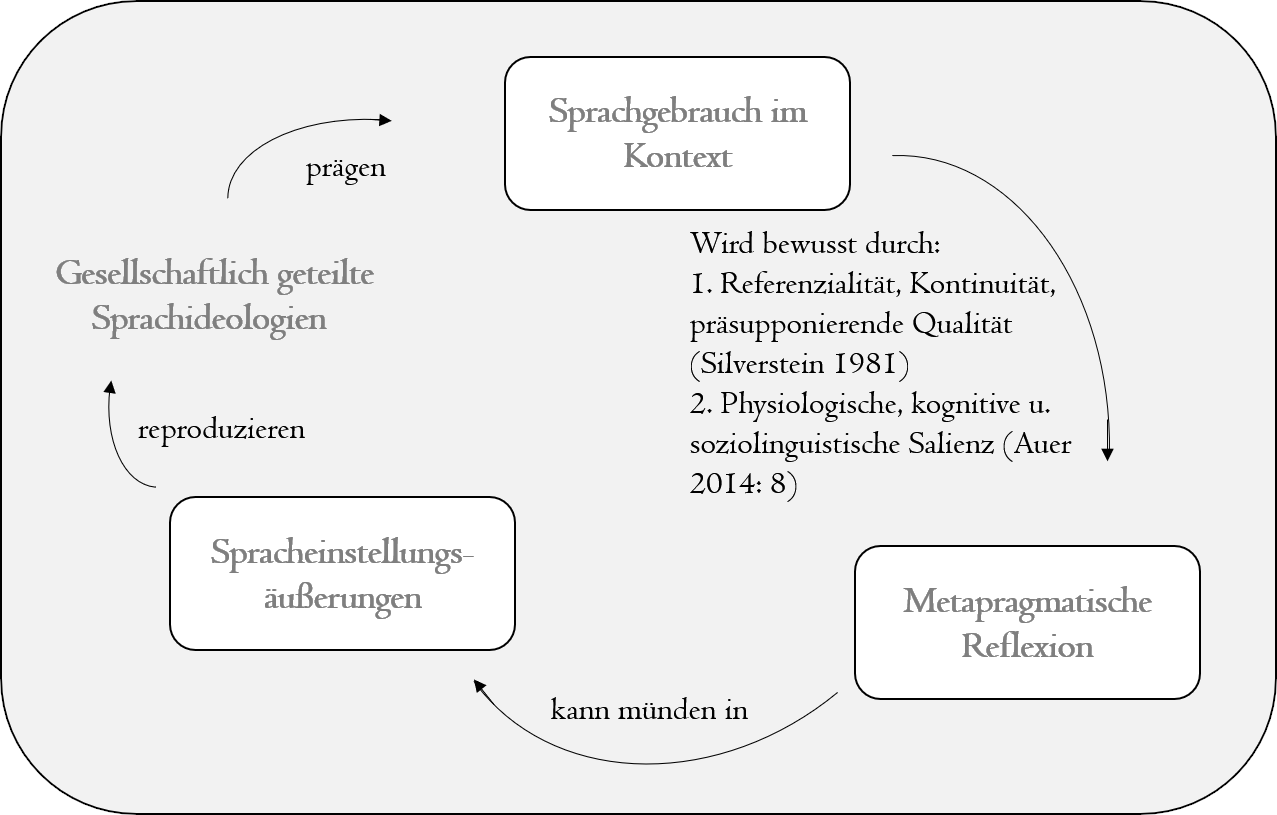
\includegraphics[width=\textwidth]{ModellMetapragmatikundSprachgebrauch}
\caption{Schematische Darstellung des Zusammenhangs von Sprachgebrauch und Metapragmatik}
\label{pic:MetapragmatikundSprachwandel}
\end{figure}
%Schaubild
Dargestellt ist, wie Sprachgebrauch, metapragmatische Bewusstheit, die Reflexion über den wahrgenommenen Sprachgebrauch und die Bewertung des Sprachgebrauchs interagieren. 
Über bestimmte sprachliche Formen reflektieren Sprachbenutzer:innen bewusst. 
Welche das sind, hängt von mehreren Faktoren ab: Einerseits nennt \citet[]{Auer2014} die Salienz, für die Eigenschaften wie etwa Phonemstatus, Frequenz und geografische Reichweite relevant sind, andererseits nennt \citet[]{Silverstein.1981} die Faktoren Referentialität, Kontinuität und präsupponierende Qualität (s. \autoref{sec:MetapragmatischeBewusstheit}). 
Die von diesen Faktoren begünstigte Auffälligkeit ist die Voraussetzung dafür, dass über ein sprachliches Zeichen bewusst reflektiert wird \citep[s.][374]{Butterworth.2011}. 
Ob etwas als auffällig wahrgenommen wird, wird immer vor dem konkreten Kontext entschieden, in dem ein sprachliches Zeichen erscheint. 
Wie dieser Kontext aufgefasst und interpretiert wird, ist wiederum mitbestimmt von sprachideologischen Vorstellungen.
Gesellschaftlich geteilte Sprachideologien bilden also gewissermaßen den Hintergrund, vor dem uns sprachliche Zeichen bewusst werden, sodass wir über sie reflektieren.
Damit sind die in einer Gesellschaft bekannten Sprachideologien und persönliche Einstellungen der Sprachbenutzer:innen zu bestimmten Formen, das Wissen über Sprache also, entscheidend dafür, welche sprachlichen Formen bewusst wahrgenommen werden. 
Die bewusste Wahrnehmung kann zu einer Reflexion führen, die ihrerseits Einstellungen und Ideologien hervorbringt, indem sie die bereits vorhandenen bestätigt, hinterfragt oder ergänzt.
Dabei sind persönliche Einstellungen wie Normbewusstheit und -toleranz entscheidend \citep[s.][375]{Butterworth.2011}. 
Die durch den Reflexions- und Bewertungsprozess generierten Sprachurteile \glqq steuern die situative Auswahl zwischen verschiedenen verfügbaren sprachlichen Varianten und wirken sich damit auf die Art des Sprachgebrauchs einer Gesellschaft aus\grqq{} \citep[372]{Butterworth.2011}.
Dieser Sprachgebrauch kann Ausgangspunkt für erneute metapragmatische Reflexion sein, evtl. mit anderen Bewertungsergebnissen, die ihrerseits wieder den Sprachgebrauch prägen. 
Somit formt Metapragmatik sprachliche Variation und damit auch sprachlichen Wandel zu einem erheblichen Maße mit. 

\chapter{Variation und Wandel der Kasusrektion von Präpositionen im Deutschen} \label{cha:SekPraeps}
Ein Phänomen, das von SprecherInnen des Deutschen stark reflektiert wird und auf das in zahlreichen Spracheinstellungsäußerungen Bezug genommen wird, sind die Variation und der Wandel im Bereich der Kasusrektion von Präpositionen. 
Zahlreiche Präpositionen des Deutschen können sowohl mit dem Genitiv als auch mit dem Dativ gebraucht werden: 
\begin{exe}
\ex \object{Das war aus meiner Sicht nur \textbf{während des} Studiums so.} (DWDS, 2000, Die Zeit)\footnote{Alle \citeauthor{DWDS}-Belege stammen aus den aggregierten Referenz- und Zeitungskorpora von 2000 bis 2018.}
\ex \object{Und \textbf{während dem} Studium an der Wirtschaftshochschule wurden sie rot.} (DWDS, 2017, Die Zeit)
\end{exe}
Die beiden Belege aus dem \citeauthor{DWDS} zeigen, dass die Präposition \waehrend{} sowohl mit dem Genitiv als auch mit dem Dativ gebraucht wird, ohne dass sich ein Unterschied in der Denotation ergeben würde. 
Dies grenzt die hier behandelten Dativ-Genitivschwankungen von Wechselpräpositionen ab, die zwischen Dativ und Akkusativ variieren und bei denen je nach Kasusrektion entweder eine Richtung (Akkusativ) oder eine Position (Dativ) denotiert wird.  
Einen Überblick über die Faktoren zu geben, die für die Variation zwischen Dativ- und Genitivrektion relevant sind, ist Ziel des folgenden Kapitels. 
Dafür ist es wichtig, zunächst einen Blick auf die grammatischen Eigenschaften von Präpositionen zu werfen. 
\autoref{sec:PraepDE} stellt daher die Wortart der Präpositionen im Deutschen vor (\autoref{sec:Wortart}) und erläutert die Einteilung in Primär- und Sekundärpräpositionen (\ref{sec:Primaer} und \autoref{sec:Sekundaer}). 
Anschließend wird in \autoref{sec:Grammatikalisierung} auf die Entstehung und Entwicklung von Präpositionen im Rahmen der Grammatikalisierungstheorie eingegangen, wobei insbesondere die vier hier untersuchten Sekundärpräpositionen (\object{wegen, während, dank} und \object{gegenüber}) berücksichtigt werden. 
In \autoref{sec:LexikGrammatik} werden zunächst allgemeine Grammatikalisierungstendenzen der Präpositionen besprochen. 
Bei der anschließend thematisierten Kasusrektion lassen sich zwei Entwicklungstendenzen beobachten: die Entwicklung von der Genitiv- zur Dativrektion und die umgekehrte Entwicklung von der Dativ- zur Genitivrektion. 
Wie in \autoref{sec:Prototypisierung} und \autoref{sec:Differenzierung} gezeigt wird, kann insbesondere die Entwicklung zur Genitivrektion nicht allein durch voranschreitende Grammatikalisierung erklärt werden. 
In \autoref{sec:IndexikalitaetRektionskasus} geht es daher um die Indexikalität der Rektionsvarianten, die einen weiteren Erklärungsfaktor darstellt. 
Hier werden korpuslinguistische Distributionen (\autoref{sec:KorpusstudienRektion}), der Registrierungsprozess in Grammatiken und sprachpflegerischen Schriften (\autoref{sec:IndexikalitaetRektionskasushistorisch}) sowie erste Überlegungen zur Reflexion im laienlinguistischen Diskurs thematisiert (\autoref{sec:IndexikalitaetRektionskasusheute}). 
Letztere erscheinen aufgrund der in \autoref{cha:SprachideologienundSpracheinstellungen} diskutierten Zusammenhänge zwischen Sprachideologien und Sprachgebrauch besonders relevant, wurden bisher in der Forschung aber selten berücksichtigt, weshalb sich die vorliegende Studie ihrer näheren Untersuchung annimmt. 
\section{Das Präpositionalsystem des Deutschen} \label{sec:PraepDE}
Präpositionen zählen zu den häufigsten Wörtern des Deutschen \citep[s.][636--637]{Griehaber2009}. 
So ist \object{in} das am zweithäufigsten gebrauchte Wort nach den Formen des Definitartikels \citep[s.][]{InstitutfurDeutscheSprache2012}. 
Gleichzeitig existiert aber eine große Zahl sehr niedrigfrequenter Vertreter wie \object{einschließlich}. 
In Bezug auf die Frequenz herrscht innerhalb der Wortart also eine große Varianz. 
Die Angaben zur Gesamtanzahl der Präpositionen im Deutschen schwanken zwischen unter 30 und ein paar Hundert, was in der Schwierigkeit begründet liegt, die Präpositionen von anderen Wortarten abzugrenzen \citep[s.][262]{Lindqvist1994}. 
Ein weiterer Grund ist die Offenheit der Wortart für neue Vertreter (\citealp[s.][526]{Eisenberg1979}; \citealp[17]{Lehmann1992}; \citealp[§896]{Duden2016}; \citealp[354]{Helbig.2017}; \autoref{sec:LexikGrammatik}).
Im folgenden Abschnitt werden die Kriterien thematisiert, die Präpositionen ausmachen. 
\subsection{Eigenschaften der Wortart Präposition} \label{sec:Wortart}
Präpositionen sind unflektierbare Funktionswörter.\footnote{Die sich zeigenden Ansätze von Flexion diskutiert \citet{Nubling2005}.} 
Sie bilden den Kopf einer Pr{\"a}positionalphrase und regieren den Kasus der darin eingebetteten Nominalphrase~(\citealp[s.][630]{Griehaber2009}; \citealp[182]{Eisenberg.2013}). 
Im Deutschen sind Präpositionen ihrem Bezugswort in den meisten Fällen vorangestellt (\object{unter dem Tisch}).\footnote{Auch in zahlreichen weiteren germanischen Sprachen stehen Präpositionen typischerweise vor der Nominalphrase. In vielen anderen Sprachen wie etwa dem Koreanischen, dem Finnischen, dem Ungarischen oder dem Hindi dominieren hingegen die Postpositionen \citep[s.][]{Dryer2013}. 
Daneben gibt es einige wenige Sprachen mit Inpositionen (etwa Anindilyakwa und Tümpisa Shoshone): Hier wird ein Element in die Nominalphrase eingefügt~\citep[s.][]{Dryer2013}.}
Es gibt allerdings auch postponierte (\object{der Umwelt zuliebe}) oder zirkumponierte (\object{um der guten Laune willen}) Vertreter. 

Als Präpositionalkasus kommt im Deutschen typenmäßig am häufigsten der Genitiv vor (z.\,B. \object{abseits, jenseits}), dann der Dativ (z.\,B. \object{bei, mit}) und schließlich der Akkusativ (z.\,B. \object{gegen, wider}) (\citealp[s. etwa][131--132]{Eroms1981}; \citealp[638]{Griehaber2009}; vgl. dazu auch \autoref{sec:Primaer} und \autoref{sec:Sekundaer}). 
Einige Präpositionen können nicht nur Nominalphrasen regieren, sondern z.\,B. auch eine andere Präpositionalphrase (\object{das ist von vor dem Krieg}). 
Pr{\"a}positionen sind nicht satzgliedf{\"a}hig, das hei{\ss}t, sie k{\"o}nnen nicht alleine ein Satzglied bilden~\citep[s.][633]{Griehaber2009}.
Als Köpfe von Präpositionalphrasen können sie aber Teile verschiedener Satzglieder sein, etwa von Adverbialen (\object{die Tasse steht auf dem Tisch}) oder von Präpositionalobjekten (\object{sie wartet auf den ICE}). 

Semantisch gesehen bringen Präpositionen Beziehungen zum Ausdruck, die z.\,B. lokal, temporal oder kausal sein können (\citealp[ausführlich dazu][]{Eroms1981}; \citealp[s. außerdem][365--366]{Jung1980}; \citealp[51--53, 55]{Rauh1990}). 
\begin{exe}
\ex \object{Ein hübsches und stolzes Paar \textbf{unter} dem Eiffelturm.} (DWDS, 2008, Die Zeit)
\ex \object{Für die Kunden einer Champagner-Firma lieferte von Klingenberg \textbf{vor} Weihnachten Geschenksträuße.} (DWDS, 2000, Die Zeit) 
\ex \object{Bei tausenden Menschen an der Golfküste fiel \textbf{wegen} des Unwetters der Strom aus.} (DWDS, 2011, Die Zeit)
\end{exe}
%Pr{\"a}positionen haben also die Funktion, zwei Größen zueinander in ein Verh{\"a}ltnis zu setzen, etwa die Tasche und den Tisch in (4)~(\citealp[s.][145]{Buscha1984}; \citealp[296]{Braunmueller1985}. 
Dabei können keineswegs nur Verhältnisse zwischen Nominalphrasen ausgedrückt werden, sondern bspw. auch ein Verh{\"a}ltnis zwischen einem Verb und einem Substantiv wie in \textit{sie liest w{\"a}hrend der Fahrt}~\citep[s.][41]{Romare.2004}.

Zwar können die bisher genannten Kriterien als Kerneigenschaften von Präpositionen angesehen werden, jedoch bilden die Präpositionen keine homogene Klasse.
Es fällt daher schwer, Kriterien zu definieren, die für alle ihre Vertreter gelten und sie scharf von anderen Wortarten, wie etwa den Konjunktionen, abzugrenzen \citep[s.][264]{Lindqvist1994}. 
So sind die Pr{\"a}position \textit{w{\"a}hrend }und die Konjunktion \textit{w{\"a}hrend }morphologisch und semantisch gleich und unterscheiden sich lediglich in syntaktischer Hinsicht~\citep[s.][39]{Romare.2004}.
%Ein größeres Problem stellen \object{als} und \object{wie} in Vergleichen dar. 
%Diese werden teils als Präpositionen, teils als Konjunktionen eingeordnet \citep[s.][41]{Romare.2004}.
%Von anderen nicht flektierbaren Wortarten sind Pr{\"a}positionen scheinbar recht leicht abgrenzbar, so weist \citet[129]{Eroms1981} darauf hin, die Abgrenzung von Interjektionen werde nicht diskutiert, da diese eine klare eigene Semantik aufwiesen. Er f{\"u}hrt jedoch an, dass bspw. das Kriterium der Kasusforderung auch bei einigen Interjektionen zu sehen sei (als Beispiel nennt er \object{weh mir})~\citep[s.][129]{Eroms1981}.

Ein Merkmal, das wie auch hier in der Literatur sehr h{\"a}ufig aufgef{\"u}hrt wird, ist die Unflektierbarkeit. 
\citet[10--11]{Lindqvist1994} weist jedoch darauf hin, dass dies in F{\"a}llen, in denen Partizipien pr{\"a}positional verwendet werden (bspw. \object{entsprechend}), problematisch sei, da es sich hierbei um flektierte Formen von Verben handele. 

Auch die wichtigste formale Eigenschaft der Präpositionen, die Rektion eines obliquen Kasus, entpuppt sich als nicht unproblematisch. 
So warnt \citet[29]{Lindqvist1994} davor, die M{\"o}glichkeit der Nominativrektion unber{\"u}cksichtigt zu lassen~(\citealp[s. auch][134]{Eroms1981}; \citealp[695]{Engel1988}). 
Bei \object{je} bspw. wird davon ausgegangen, dass die Pr{\"a}position neben dem Akkusativ auch den Nominativ regieren kann~\citep[s.][291]{Hentschel1989}. 
%Die Grenzfälle \object{als} und \object{wie} sowie auch \object{außer} können als Präpositionen ohne Kasusforderung gesehen werden \citep[so etwa bei][73]{Wunderlich1984}, sind dann aber von den Konjunktionen kaum noch abzugrenzen \citep[s.][]{BELEG}. 
%Auch \object{bis} wird häufig als Präposition ohne Kasusforderung eingestuft \citep[s. etwa][76, 83--84]{Wunderlich1984}. 
\citet[291]{Hentschel1989} f{\"u}hrt zudem an, dass es wegen Synkretismusvermeidung h{\"a}ufig zur Nullflexion nach Pr{\"a}positionen kommt, wenn die Nominalphrase nur aus einem Substantiv ohne Erweiterung besteht (\textit{der Unterschied zwischen Affe und Mensch}). 

\citet{Lindqvist1994} vertritt die Auffassung, eine klare Abgrenzung der Pr{\"a}positionen von anderen Wortarten sei in vielen F{\"a}llen nicht m{\"o}glich.
%Hinweise auf die Schwierigkeit der Trennung finden sich auch etwa bei ,\citet[Quelle?]{Paul1920}, \citet[Quelle?]{Behagel1924} und \citet[Qualle?]{Braunmueller1982}. 
Statt einer starren Einteilung schl{\"a}gt er daher ein Modell vor, bei dem die infrage kommenden W{\"o}rter entlang einer Skala angeordnet werden~\citep[s.][5]{Lindqvist1994}. 
Auf diese Weise lässt sich zwischen prototypischen Vertretern der Wortart und peripheren Mitgliedern unterscheiden. 
Dieser Ansatz soll auch hier verfolgt und in den folgenden beiden Abschnitten näher erläutert werden. 
\subsection{Prototypische Präpositionen} \label{sec:Primaer}
Betrachtet man das Präpositionalsystem des Deutschen, lässt sich eine Gruppe prototypischer Präpositionen wie \object{in}, \object{auf}, oder \object{an} ausmachen, die den Kern der Wortart darstellt \citep[s.][214]{DiMeola2011}. 
Die Gruppe umfasst nur etwa 20 Mitglieder, die als Primärpräpositionen bezeichnet werden \citep[s.][94]{Szczepaniak2011}.\footnote{\citet[146]{Buscha1984} spricht von 40 Primärpräpositionen, die er allerdings nicht einzeln aufführt.}  
Als Prototyp lassen sich die Primärpräpositionen vor allem aufgrund ihrer hohen Frequenz auffassen (\citealp[s.][631]{Griehaber2009}; \citealp[94]{Szczepaniak2011}; \citealp[§896]{Duden2016}).
So gehören etwa die Primärpräpositionen \object{in, von} und \object{mit} zu den zehn häufigsten Wörtern des Deutschen \citep[s.][]{InstitutfurDeutscheSprache2012}. 
\autoref{table:FrequenzPraepositionen} listet die 20 Primärpräpositionen nach ihrer Frequenz laut der Wortgrundformenliste (DeReWo) des IDS auf sowie im Vergleich die Frequenz der vier in dieser Studie untersuchten Sekundärpräpositionen.
% Please add the following required packages to your document preamble:
% \usepackage{multirow}
% \usepackage[table,xcdraw]{xcolor}
% If you use beamer only pass "xcolor=table" option, i.e. \documentclass[xcolor=table]{beamer}
\begin{table}
\begin{tabular}{llr}
\lsptoprule
       & Präposition           & Häufigkeitsklasse \\\midrule
primär & \object{in}           & 2              \\
       & \object{von}          & 3              \\
       & \object{mit}          & 3              \\
       & \object{für}          & 4              \\
       & \object{auf}          & 4              \\
       & \object{zu}           & 4              \\
       & \object{an}           & 4              \\
       & \object{bei}          & 4              \\
       & \object{nach}         & 5              \\
       & \object{aus}          & 5              \\
       & \object{über}         & 6              \\
       & \object{vor}          & 6              \\
       & \object{durch}        & 6              \\
       & \object{gegen}        & 6              \\
       & \object{um}           & 6              \\
       & \object{bis}          & 6              \\
       & \object{zwischen}     & 7              \\
       & \object{seit}         & 7              \\
       & \object{ab}           & 7              \\
       & \object{unter}        & 7              \\\midrule
sekundär  & \object{wegen}     & 8              \\
          & \object{während}   & 8              \\
          & \object{gegenüber} & 9              \\
          & \object{dank}      & 11             \\
\lspbottomrule
\end{tabular}
\caption{Die 20 Primärpräpositionen und die vier hier untersuchten Sekundärpräpositionen nach Frequenz (Frequenzangaben aus \citealt{InstitutfurDeutscheSprache2012})}
\label{table:FrequenzPraepositionen}
\end{table}

Die Frequenzen in der Wortgrundformenliste basieren auf dem Deutschen Referenzkorpus (DeReKo) und werden in Häufigkeitsklassen angegeben: \glqq Dabei hat ein Wort die
Häufigkeitsklasse N, wenn das häufigste Wort etwa 2$^{N}$-mal häufiger vorkommt als dieses Wort\grqq{} \citep[13]{InstitutfurDeutscheSprache2012}. 
Das häufigste Wort sind die Determiniererformen \object{der}, \object{die} und \object{das}. 
Das zweithäufigste Wort, die Präposition \object{in}, kommt bereits nur noch um ein Vierfaches seltener vor.\footnote{Klitisierte Formen wie \object{im} sind in der Wortgrundformenliste gesondert aufgeführt, werden hier aber nicht mit aufgenommen.} 
Hier zeigt sich die für Häufigkeitsverteilungen in der Sprache typische Zipf-Kurve: Nur wenige Präpositionen kommen sehr häufig vor, während die große Mehrzahl der Präpositionen selten ist \citep[s.][22--27]{Zipf.1972}.

Bei den Primärpräpositionen handelt es sich nicht nur um die frequentesten, sondern auch um die ältesten Vertreter der Wortart. 
Sie werden bereits seit dem Althochdeutschen gebraucht~\citep[s.][1]{Graff.1824}.
Ein weiterer Hinweis auf den Charakter der Primärpräpositionen als prototypische Vertreter der Wortart ist ihr früher Erwerb \citep[s.][203--206]{Becker2011}. 

Neben diesen prototypischen Primärpräpositionen finden sich sprachhistorisch neue Präpositionen, die Sekundärpräpositionen.
Zu dieser Gruppe gehören die hier untersuchten Präpositionen \object{dank}, \object{wegen}, \object{während} und \object{gegenüber}. 
Sekund{\"a}rpr{\"a}positionen sind im Vergleich zu Prim{\"a}rpr{\"a}positionen deutlich weniger tokenfrequent~\citep[636--637]{Griehaber2009}.
\object{Wegen} ist unter den Sekundärpräpositionen eine der häufigsten und steht in der DeReWo-Wortgrundformenliste auf Platz acht, zusammen mit Wortformen wie \object{Haus} und \object{ihm} \citep[s.][]{InstitutfurDeutscheSprache2012}. 
Die Gruppe hat aber eine große Anzahl an Vertretern, ist also sehr viel typenfrequenter \citep[s.][93]{Szczepaniak2011}.

Von den Sekundärpräpositionen lassen sich noch einmal die Tertiärpräpositionen unterschieden \citep[s.][631]{Griehaber2009}. 
Hierbei handelt es sich um Einheiten, die aufgrund ihres peripheren Status als Präpositionen in Verbindung mit einer Primärpräposition stehen müssen, über die sie den Kasus einer Nominalphrase regieren, wie \object {im Hinblick auf} oder \object{in Verbindung mit}. 
Mit dieser zusammen bilden sie dann eine neue präpositional verwendete Einheit. 

Prim{\"a}r-, Sekund{\"a}r- und Tertiärpr{\"a}positionen stellen keine distinkten Gruppen dar, sondern sollten, wie \citet[261]{Lindqvist1994} in seiner Untersuchung zu Präpositionen im Deutschen und Schwedischen argumentiert, als Kontinuum gesehen werden.\footnote{\citet[18--21]{Lindqvist1994} merkt an, dass die Darstellung anhand einer Skala nicht implizieren soll, dass allen Parametern tats{\"a}chlich nat{\"u}rliche Skalen zugrunde liegen. 
So l{\"a}sst sich etwa der Wechsel von der Nach- zur Voranstellung nur als skalare Ver{\"a}nderung auffassen, wenn der Bezugspunkt der idealisierte Prototyp einer Präposition ist.
Zudem können innerhalb der einzelnen Parameter Ver{\"a}nderungen durchaus sprunghaft stattfinden. Manche Parameter wie etwa die L{\"a}nge einer Pr{\"a}position lassen sich zwar kontinuierlich darstellen, dabei ist aber zu beachten, dass es sich hier nicht um kontinuierliche Skalen handelt, sondern der Wandel in kleinen Spr{\"u}ngen stattfindet.}
Das Pr{\"a}positionalsystem ist also prototypisch organisiert~\citep[s.][33--34]{Bene.1975}. 

Auch nach außen hin sind Präpositionen kaum klar abgrenzbar, wie in \autoref{sec:Wortart} bereits angeklungen ist. 
Daher schlagen bereits \citet{Quirk.1964} vor, keine scharfe Abgrenzung von Pr{\"a}positionen und anderen Wortarten vorzunehmen. 
Auf diese Weise geht auch \citet[]{Lindqvist1994} vor: Er fragt nicht danach, ob eine Einheit eine Präposition ist oder nicht, sondern verfolgt einen Prototypenansatz, indem er danach fragt, wie nah die Einheit an der prototypischen Präposition ist \citep[s.][13]{Lindqvist1994}. 
Hierfür definiert er ein sogenanntes Idealpräpositionale, also das Ideal\-modell einer Pr{\"a}position \citep[s.][15--16]{Lindqvist1994}. 
Dieses Idealpräpositionale weist Eigenschaften auf, die prototypische Vertreter der Präpositionen in der Regel teilen. 
Dazu geh{\"o}ren sowohl formale als auch funktionale Eigenschaften. 
Auf der formalen Seite sticht vor allem die Kürze ins Auge: Prototypische Präpositionen sind meistens einsilbig und haben eine simple Silbenstruktur \citep[s.][§899]{Duden2016}. 
Ausnahmen wie \object{über} und \object{unter} weichen von dieser Einsilbigkeit ab und stehen dem Prototyp somit weniger nah als \object{auf} oder \object{mit}.
Mit ihrer Kürze hängt eng zusammen, dass Primärpräpositionen morphologisch nicht segmentierbar sind \citep[s.][33]{Lehmann1992}. 
Wie oben bereits erwähnt, gehört auch die Voranstellung zu den prototypischen Eigenschaften.  
Eine wesentliche funktionale Eigenschaft prototypischer Präpositionen ist die semantische Vielwertigkeit \citep[s.][15]{Lindqvist1994}. 
Primärpräpositionen können oft neben einer konkreten lokalen Bedeutung sehr abstrakte grammatische Bedeutungen haben (\object{auf dem Tisch stehen} vs. \object{auf den Bus warten}).\footnote{\citet[10--11]{Lehmann1992} unterscheiden innerhalb der Primärpräpositionen noch eine weitere Gruppe, nämlich grammatische Präpositionen wie \object{von} und \object{zu}.}
Auch syntaktisch sind Primärpräpositionen vielwertig.
Bspw. können sie zum Teil als Verbpartikeln (\textit{aufessen, anschalten, mitgehen}) und in Pronominaladverbien (\textit{darauf, darin}) auftreten~\citep[s.][275--276]{Lindqvist1994}.  
Zudem können Prim{\"a}rpr{\"a}positionen selbst regiert werden von Substantiven (\textit{Glaube an}), Adjektiven (\textit{reich an}), komplexen Pr{\"a}positionen (\textit{mithilfe von}) oder als Einleiter von Präpositionalobjekten von Verben (\textit{warten auf}) ~(\citealp[s.][39]{Lehmann1992};  \citealp[68]{Diewald.1997}).

Die für die vorliegende Untersuchung wichtigste Eigenschaft der Präpositionen ist ihr Rektionskasus. 
Dieser ist bei den Primärpräpositionen der Dativ oder der Akkusativ \citep[s.][94]{Szczepaniak2011}. 
Eine besondere Gruppe innerhalb der Primärpräpositionen bilden die Wechselpräpositionen \object{in, auf, an, über, vor, unter, zwischen, neben, hinter} (\citealp[s.][§912--913]{Duden2016}, hier geordnet nach der Frequenz in einer Korpusuntersuchung im LIMAS-Korpus von~\citealp[19]{Folsom1984}). 
In der Regel gilt für die Wechselpräpositionen, dass sie den Dativ regieren, wenn auf eine statische Position referiert wird, während sie den Akkusativ regieren, wenn eine Richtungsbewegung beschrieben wird \citep[s.][§912]{Duden2016}. 
\begin{exe}
\ex \object{Er hätte \textbf{auf dem} Podest stehen können.} (DWDS, 2005, Berliner Zeitung) 
\ex \object{Erstmals in dieser Saison \textbf{auf das} Podest schaffte es der Tscheche Lukas Hlava als Dritter.} (DWDS, 2012, Die Zeit)
\end{exe}
Wenn in dieser Studie von Rektionsvarianten gesprochen wird, sind die verschiedenen Rektionsmöglichkeiten der Wechselpräpositionen nicht gemeint, da diese Möglichkeiten semantisch gesteuert sind \citep[s.][703]{Engel1988}.
\subsection{Peripherie der Wortart}
\label{sec:Sekundaer}
Nachdem nun die prototypischen Vertreter der Wortart Präposition vorgestellt wurden, wird im folgenden Abschnitt auf die Peripherie der Wortart eingegangen, insbesondere auf die Gruppe der Sekundärpräpositionen. 
Sekundärpräpositionen sind sprachhistorisch jünger als Primärpräpositionen. 
In einer Korpusuntersuchung zu Präpositionen im Mittelhochdeutschen von \citet[]{Waldenberger.2009} kommt keine der hier untersuchten Pr{\"a}positionen \object{wegen}, \object{während}, \object{dank} und \object{gegenüber} vor. 
Wann genau die Entwicklung komplexer Pr{\"a}positionen begonnen hat, ist unklar, vermutet wird aber, dass dies im Fr{\"u}hneuhochdeutschen der Fall war~\citep[s.][50]{Meibauer1995}. 
\citet[43]{Romare.2004} geht davon aus, dass Sekundärpräpositionen ab dem Sp{\"a}tmittelalter entstehen. 

Sekundärpräpositionen verfügen im Vergleich mit Primärpräpositionen über eine spezifischere eigene Semantik, die aber bereits zu verblassen beginnt (\autoref{sec:LexikGrammatik}). 
So lässt sich etwa die Bedeutung von \object{einschließlich} genauer umschreiben als die von \object{in}. 
\citet[42--43]{Bene.1975} f{\"u}hrt daher die explizitere Beschreibung der Relation als einen Grund f{\"u}r die Verwendung neuer Pr{\"a}positionen an. 
Laut \citet[67]{Diewald.1997} beschreiben sie Relationen, {\glqq}die übereinzelsprachlich gesehen selten oder nie vollst{\"a}ndig grammatikalisiert werden{\grqq}. 
\citet{Eisenberg1979} pl{\"a}diert aufgrund ihrer konkreten Semantik f{\"u}r einen lexikalischen Status der morphologisch komplexen Pr{\"a}positionen.

Auf formaler Seite unterscheiden sich die Sekundärpräpositionen von den Primärpräpositionen insbesondere dadurch, dass sie sich in mehrere Morpheme zerlegen lassen oder zumindest morphologisch transparent sind \citep[s.][62]{DiMeola2001}. 
So weist \object{mithilfe} die Morpheme \{mit\} und \{hilfe\} auf. 
Auch \object{während} ist segmentierbar (\{währen\} + \{d\}). 
Sekundärpräpositionen wie \object{dank} oder \object{trotz} lassen sich zwar nicht weiter segmentieren, weisen aber morphologische Transparenz auf, da sie mit Substantiven oder Verbstämmen identisch sind, aus denen sie sich entwickelt haben. 

Während die Primärpräpositionen vorangestellt werden, gibt es unter den Sekundärpräpositionen einige Vertreter, die nachgestellt oder zirkumponiert sind \citep[s.][152]{DiMeola2000}.
\begin{exe}
\ex \object{Erlaubt waren dabei dem Regelwerk \textbf{entsprechend} 100 Kilometer.} (DWDS, 2012, Die Zeit)
\ex \object{Familienpolitik muss aber \textbf{um} der Kinder \textbf{willen} gemacht werden.} (DWDS, 2002, Berliner Zeitung)
\end{exe}
Zudem variieren einige Sekundärpräpositionen zwischen Voran- und Nachstellung oder sogar zwischen Voran-, Nach- und Zirkumstellung, etwa (\object{von}) \object{wegen}. 
\begin{exe}
\ex \object{Insgesamt fielen \textbf{wegen} des Streiks mehr als 1500 Flüge aus. } (DWDS, 2012, Die Zeit)
\ex \object{Die besten unserer Amtsträger kandidieren nicht des Geldes \textbf{wegen}.} (DWDS, 2013, Die Zeit) 
\ex \object{Deshalb gehört solchen Tendenzen \textbf{von} Gesetzes \textbf{wegen} ein Riegel vorgeschoben.} (DWDS, 2000, Der Tagesspiegel)
\end{exe}
In den syntaktischen Funktionen, die sie ausfüllen können, sind die Sekundärpräpositionen eingeschränkter als die Primärpräpositionen, da sie keine Präpositionalobjekte einleiten können. 
Anders als mit Primärpräpositionen können mit Sekundärpräpositionen außerdem keine Pronominaladverbien gebildet werden \citep[s.][526]{Eisenberg1979}.  

%\begin{quote}W{\"a}hrend die morphologisch einfachen (alten) Pr{\"a}positionen Proforrnen mit pr{\"a}figierten \textit{da(r) (davor, darin) }bilden, ben{\"o}tigen die morphologisch komplexen den nachgestellten Genitiv des Relativpronomens \textit{(infolge dessen, anhand deren).}~\citep[526]{Eisenberg1979}\end{quote}
Betrachtet man die Kasusrektion der Sekundärpräpositionen, so fällt auf, dass hier neben der Dativ- und der Akkusativrektion auch die Genitivrektion möglich ist.\footnote{Daneben kommen Präpositionen vor, die keinen bestimmten Kasus regieren, also mit allen Kasus auftreten können, wie etwa \object{minus}~(\citealp[40--41]{Lindqvist1994}; \citealp[§919]{Duden2016}). Ob Einheiten wie \object{minus} oder \object{plus} zu den Präpositionen gerechnet werden sollten, ist fraglich, soll hier jedoch nicht weiter diskutiert werden.} 
Der Genitiv ist unter den Sekundärpräpositionen sogar der am häufigsten regierte Kasus \citep[s.][16]{Lehmann1992}. 
Aufgrund der hohen Typenfrequenz der Sekundärpräpositionen hat die Genitivrektion damit insgesamt die höchste Typenfrequenz unter den Präpositionen (\citealp[s.][131--132]{Eroms1981}; \citealp[638]{Griehaber2009}). 
Sehr häufig variieren die Sekundärpräpositionen in ihrer Kasusrektion, meist zwischen Genitiv und Dativ (\citealp[s.][§910]{Duden2016}; \citealp[zu Schwankungen bei historisch neuen Akkusativpr{\"a}positionen wie etwa \textit{pro} s.][]{Hentschel1989}). 
\citet[32]{Lindqvist1994} nennt ca. 40~Pr{\"a}positionen, die ausschlie{\ss}lich den Genitiv regieren können und keine Variation aufweisen (etwa \textit{bar, zuz{\"u}glich, kraft, im Laufe}). 
Für die meisten Sekundärpräpositionen, auch für einige der von \citet{Lindqvist1994} genannten, lassen sich jedoch Belege für verschiedene Rektionsvarianten finden, wie \citeauthor[]{DiMeola2000} in Korpusuntersuchungen zeigt (s. etwa \citeyear[]{DiMeola1999}; \citeyear{DiMeola2000}; \citeyear{DiMeola2006}). 
Anders als bei den Wechselpräpositionen ist diese Variation nicht im engeren Sinne semantisch gesteuert, d.\,h. es gibt auf der denotativen Ebene keinen Unterschied zwischen Varianten wie \object{während des Studiums} und \object{während dem Studium}. 
Der \citet[]{Duden2016} schreibt dazu: 
\begin{quote}Einige Pr{\"a}positionen schwanken in ihrer Rektion, ohne dass dies Einfluss auf ihre Bedeutung h{\"a}tte. Hier vollzieht sich Sprachwandel (man spricht von Nebenkasus): \object{wegen des Geldes (Genitiv) / wegen dem Geld (Dativ); dank ihres Einsatzes / dank ihrem Einsatz}~\citep[{\S}910]{Duden2016}\end{quote}
Dass beide Varianten von SprachbenutzerInnen allerdings sehr unterschiedlich bewertet werden, ist Thema dieser Studie und wird in \autoref{sec:IndexikalitaetRektionskasusheute} näher beleuchtet. 
In einigen Fällen wird die Dativrektion auch durch die syntaktische Umgebung begünstigt. 
So kommt der Dativ bspw. häufig vor, wenn sonst zwei Genitivphrasen aufeinanderfolgen würden (\object{während dem Korrigieren des Buchs} oder \object{während Tims langem Aufenthalt}). Folgt ein Substantiv ohne Determinierer auf die Präposition, bleibt es häufig endungslos (\object{wegen Umbau}) \citep[s.][§917--918]{Duden2016}. 

\autoref{table:Kontinuum} zeigt zusammenfassend die besprochenen formalen und funktionalen Unterschiede zwischen Primär- und Sekundärpräpositionen und führt daneben auch die Eigenschaften der Tertiärpräpositionen auf. 
\begin{table}
\begin{small}
\centering
\begin{tabular}{lcrll}
\lsptoprule
 \textcolor{gray}{Tertiärpräpositionen}           & \ Sekundärpräpositionen \                                            & Primärpräpositionen                     \\
 \midrule
\textcolor{gray}{Rektion über} & Genitivrektion überwiegt, & Dat.- und/oder Akk.-\\\textcolor{gray}{Primärpräposition} &aber auch Dat.- oder & Rektion\\&Akk.-Rektion         \\
\textcolor{gray}{prä-, zirkum-} & schwankend & präponiert \\\textcolor{gray}{oder postponiert} & & \\
\textcolor{gray}{mehrsilbig}                  & mehr- oder einsilbig                                            & einsilbig                               \\
\textcolor{gray}{morphologisch komplex} \ \           & \ \ morphologisch segmentierbar \ \                                       & morphologisch nicht \\ & oder transparent & weiter unterteilbar  \\
\textcolor{gray}{eher lexikalische}    & Semantik verblasst                                              & eher grammatische \\\textcolor{gray}{Bedeutung}   & &Bedeutung        \\
\textcolor{gray}{synt. Funktionen} & mehr synt. Funktionen & vielfältige synt. \\ \textcolor{gray}{eingeschränkt} & & Funktionen\\
\lspbottomrule
\end{tabular}
\end{small}
\caption{Formale und funktionale Eigenschaften von Primär-, Sekundär- und Tertiärpräpositionen}
\label{table:Kontinuum}
\end{table}

%Die Frage, ob es sich bei den Pr{\"a}positionen um eine offene oder geschlossene Wortklasse handelt, lässt sich also nicht für die gesamte Wortart beantworten, da zwischen den verschiedenen Typen von Präpositionen unterschieden werden muss \citep[s.][523]{Eisenberg1979}. 
%Insbesondere in früheren Arbeiten wurde von der Geschlossenheit der Wortart ausgegangen \citep[s. z.\,B.][]{Langacker1968}. 
%Im Strukturalismus wurden Pr{\"a}positionen als geschlossene Klasse eingeordnet, wofür laut \citet[34]{Rauh1990} insbesondere drei Argumente herangezogen wurden: \glqq 1. Präpositionen sind Funktions- oder Strukturwörter, 2. Präpositionen haben geringe lexikalische Bedeutung, 3. Die Menge der Präpositionen ist begrenzt und zeigt in einer Sprache diachronisch kaum Veränderungen.\grqq{} 
%Zu letzterem Argument führt sie an: {\glqq}Offensichtlich sind solche {\"A}u{\ss}erungen allein unter Ber{\"u}cksichtigung der in der Tag {\"u}berschaubaren Menge von urspr{\"u}nglichen oder prim{\"a}ren Pr{\"a}positionen gemacht worden{\grqq}~\citep[42]{Rauh1990}.
%\citet{Rauh1990} zeigt an Präpositionen des Englischen beispielhaft, dass diese Argumentation und demzufolge auch die Einteilung als geschlossene Klasse unangemessen ist und spricht selbst von einer \glqq potentiell unendlichen Menge von Präpositionen\grqq{}~\citep[55]{Rauh1990}. 
%Auch \citet[148]{Vestegaard.1973} sieht die Präpositionen im Englischen als produktiv an.\\ 
%Im Deutschen zeigt sich die Produktivität etwa darin, dass die Gruppe der Präpositionen Lehnwörter zulässt (\object{pro, via, versus} etc.) \citep[s.][197]{DiMeola2009}. 
%Auch die Verschmelzung von Pr{\"a}position und Substantiv, wie etwa bei \textit{mit Hilfe/mithilfe }zu beobachten, ist ein produktives Muster~\citep[s.][520]{Eisenberg1979}.  
%\citet{Eisenberg1979} stellt die Frage, warum die Gruppe der Pr{\"a}positionen st{\"a}ndig erweitert wird. 
%Den von ihm konstatierten zunehmenden Gebrauch von Pr{\"a}positionalobjekten sieht er nicht als Grund, da keine Sekund{\"a}r- oder Terti{\"a}rpr{\"a}position ein Pr{\"a}positionalobjekt einleiten k{\"o}nne \citep[524]{Eisenberg1979}.
Wie oben bereits erwähnt, handelt es sich bei den Sekundärpräpositionen (wie auch bei den Tertiärpräpositionen) um eine offene Klasse, die neue Vertreter aufnehmen kann. 
Das folgende Kapitel behandelt die Entstehung neuer Präpositionen und ihre Entwicklung insbesondere bezüglich der Kasusrektion. 
%\citet[]{Bene.1975} sieht folgenden Grund für das Hinzukommen neuer Sekundär- und Tertiärpräpositionen (bei ihm Halbpräpositionen): 
%\begin{quote}Die Halbpr{\"a}positionen bereichern das Inventar der modernen Schriftsprache. Der Hauptgrund, weshalb sich ihr Repertoire in der neueren Zeit st{\"a}ndig erweitert und erneuert, liegt wohl in ihrer semantischen Pr{\"a}gnanz.~\citep[44]{Bene.1975}\end{quote}
%Sekundär- und Tertiärpräpositionen können also als expressiver gelten, was ihre Verwendung in bestimmten Kontexten begünstigt \citep[s.][102]{Szczepaniak2011}. 
%Der Wunsch nach Expressivität kann als Motor für Sprachwandel angesehen werden uns stößt auch im Bereich der Präpositionen Grammatikalisierungsprozesse an \citep[s.][103]{Szczepaniak2011}.
%Diese Prozesse sind Thema des folgenden Kapitels. 
\section{Grammatikalisierung der Präpositionen}\label{sec:Grammatikalisierung}
In \autoref{sec:Primaer} und \autoref{sec:Sekundaer} wurden historisch alte Primärpräpositionen und historisch neue Sekundärpräpositionen aus synchroner Perspektive gegenübergestellt. 
In den folgenden beiden Abschnitten wird nun ein diachroner Blick eingenommen, der darauf abzielt, die bereits angesprochene synchron zu beobachtende Variation im Bereich der Rektion vor dem Hintergrund der historischen Entwicklung der Präpositionen zu beleuchten.

Mit Fragen des Sprachwandels im Bereich der Präpositionen haben sich bisher vor allem zahlreiche Arbeiten im Rahmen der Grammatikalisierungstheorie beschäftigt \citep[etwa][]{Lehmann1992, Lindqvist1994,  DiMeola2000, Szczepaniak2011}. 
Inwiefern sich die Entwicklungen der Präpositionen im Deutschen mithilfe der Grammatikalisierungstheorie erklären lassen, wird im Folgenden erörtert. \autoref{sec:LexikGrammatik} gibt zunächst einen Überblick über die bei der Grammatikalisierung ablaufenden Prozesse. 
\autoref{sec:Prototypisierung} und \autoref{sec:Differenzierung} widmen sich zwei Erklärungsansätzen für die Wandeltendenzen im Bereich der Rektion, wobei vor allem auf die Entwicklung der vier hier behandelten Sekundärpräpositionen \object{wegen}, \object{während}, \object{dank} und \object{gegenüber} eingegangen wird. 
Insbesondere die Arbeiten von \citeauthor{DiMeola2000} (v.\,a. \citeyear{DiMeola1998}, \citeyear{DiMeola2001}, \citeyear{DiMeola2001}, \citeyear{DiMeola2003},  \citeyear{DiMeola2004} und \citeyear{DiMeola2011}) sind dabei von Relevanz.  
\subsection{Von der Lexik in die Grammatik}
\label{sec:LexikGrammatik}
Die Grammatikalisierung eines sprachlichen Zeichens ist seine Entwicklung von einem (eher) lexikalischen Zeichen zu einem (eher) grammatischen oder von einem weniger grammatischen zu einem stärker grammatischen (\citealp[s.][303]{Lehmann.1985}; \citeyear[193]{Lehmann.1991}; \citealp[2]{Heine.1991}). 
Der Übergang zu einem grammatischen Zeichen geschieht nicht abrupt, sondern lässt sich mit dem Muster A>A/B>B modellieren (\citealp[s.][107]{Heine.1991}; \citealp[15]{Lehmann.1995}). 
Das heißt, in einer Übergangsphase kommt es auf funktionaler wie auf formaler Seite zu Variation. 
Dies zeigt sich auch bei den Sekundärpräpositionen, die etwa in ihrer Kasusrektion variieren (\autoref{sec:Sekundaer}). 

Präpositionen können zu den grammatischen Zeichen gezählt werden, da sie eine relationale Bedeutung haben \citep[s.][93]{Szczepaniak2011}. 
Dennoch werden sie von einigen als lexikalische oder teilweise lexikalische Zeichen gesehen. 
Für \citet[2076]{Zifonun1997} etwa handelt es sich bei Präpositionen um lexikalische Zeichen: \glqq W{\"a}ren Pr{\"a}positionen nur grammatisch-strukturelle Morpheme, so w{\"a}re die Offenheit der Klasse kaum zu erkl{\"a}ren\grqq. 
Auch \cite{Rauh1990} plädiert für den lexikalischen Status. 
\citet[182]{Eisenberg.2013} sieht die morphologisch komplexen Pr{\"a}positionen als lexikalisch an \citep[s. auch][]{Eisenberg1979}. 
\citet[136]{Eroms1981} schreibt Präpositionen sowohl einen grammatischen als auch einen lexikalischen Bedeutungsanteil zu.
\citet[42]{Romare.2004} sieht die Präpositionen zwar insgesamt als grammatische Klasse, bezeichnet ihre Funktion aber teils als lexikalisch, indem sie z.\,B. r{\"a}umliche Bedeutungen als lexikalisch einordnet, die Einleitung von Pr{\"a}positionalobjekten hingegen als grammatisch.
Die vorliegende Studie schließt sich der Grammatikalisierungsforschung an und betrachtet Präpositionen aufgrund ihrer relationalen Bedeutung als grammatische Zeichen. 
Dabei ist auch hier von einem Kontinuum auszugehen: Mit \citet[16, 306]{Lindqvist1994} lässt sich festhalten, dass typische Präpositionen eher grammatische Bedeutung haben, während untypische Präpositionen auch lexikalisch sein können.   
Auch die von einigen als lexikalisch eingeordnete lokale Bedeutung kann als grammatisch aufgefasst werden, was sich mit der Existenz lokativer Kasus in Sprachen wie dem Türkischen oder dem Lateinischen begründen lässt. 

Während SprachbenutzerInnen beim Gebrauch lexikalischer Zeichen recht frei sind, unterliegt der Gebrauch grammatischer Zeichen festeren Regeln. 
So kann in dem Satz \object{das Kaninchen hoppelt/hüpft/rennt über das Feld} je nach Intention zwischen den unterschiedlichen Verben gewählt werden, wohingegen die Verbendung für die dritte Person Singular obligatorisch ist.  
Die Grammatikalisierung eines Zeichens wird von \citet[130]{Lehmann.1995} daher als der Verlust an Autonomie gefasst: 
Sowohl auf der paradigmatischen Ebene als auch auf der syntagmatischen Ebene wird ein Zeichen im Laufe seiner Grammatikalisierung weniger eigenständig. 
Um dies systematisch zu beschreiben, entwickelt \citet[305]{Lehmann.1985} die drei Grammatikalisierungsparameter Gewicht, Kohäsion und Variabilität. 
Bei jedem Parameter wird zwischen paradigmatischen und syntagmatischen Aspekten unterschieden \citep[s.][131]{Lehmann.1995}. 
\autoref{table:Grammatikalisierungsparameter}  bietet eine Übersicht über die Lehmannschen Grammatikalisierungsparameter, die nun der Reihe nach vorgestellt werden.  
\begin{table}
\centering
\begin{tabular}{lccr}
\lsptoprule
                 & paradimatisch & syntagmatisch  & \\
                 \midrule
Gewicht     & Integrität           & struktureller Skopus & (nimmt ab) \\
Kohäsion   &   Paradigmatizität   &  Fügungsenge & (nimmt zu) \\
Variabilität  & Wahlfreiheit        & Stellungsfreiheit  & (nimmt ab)\\
\lspbottomrule
\end{tabular}
\caption{Grammatikalisierungsparameter nach \citet[132]{Lehmann.1995}}
\label{table:Grammatikalisierungsparameter}
\end{table}

Der Parameter Gewicht wird von \citet[]{Lehmann.1985} auf paradigmatischer Ebene als Integrität eines Zeichens bezeichnet, auf syntagmatischer Ebene als struktureller Skopus. 
Die Integrität, also das paradigmatische Gewicht eines Zeichens, betrifft sowohl seine funktionale Seite als auch seine formale Seite \citep[s.][305]{Lehmann.1985}: Die Semantizität und die Länge eines Zeichens nehmen im Laufe der Grammatikalisierung ab. 
Wie oben bereits erwähnt (\autoref{sec:Sekundaer}) bilden die Präpositionen eine relativ offene Wortart, die gut neue Vertreter aufnehmen kann \citep[518]{Eisenberg1979}. 
Neue Präpositionen können aus Adjektiven (\object{zuzüglich}), Adverbien (\object{links}), Partizipien (\object{entsprechend}), Substantiven (\object{kraft}) oder auch aus Präpositionalphrasen (\object{aufgrund}) entstehen (\citealp[s.][66]{DiMeola2001}; \citealp[215]{DiMeola2011}; vgl. auch \citealp{Braunmueller1985}).
Insbesondere Substantive und Verben sind auch sprach{\"u}bergreifend typische Spenderbereiche f{\"u}r Pr{\"a}positionen~(\citealp[672]{Kortmann.1992}; \citealp[512]{Konig.2012}). 
Am Beginn des Entwicklungsprozesses stehen also lexikalische Einheiten. 
Historisch neue Präpositionen, die aus diesen Einheiten entstehen, verfügen daher zunächst über eine recht spezifische Semantik. 
Im Gegensatz dazu erfüllen historisch alte, prototypische Präpositionen wie \object{auf} oft {\"a}hnliche Funkionen wie Kasus~(\citealp[s.][45]{Rauh1990}; \autoref{sec:Primaer}). 
Besonders deutlich ist dies bei der Präposition \object{von} zu sehen, die häufig anstelle eines Genitivs vorkommt (\object{das Buch von Johanna}) und sich damit in Richtung eines Kasusmarkers entwickelt \citep[s.][6]{Lehmann1992}. 
Auf der funktionalen Seite lässt sich also ein Verlust an Semantik ausmachen, der als Desemantisierung bezeichnet wird \citep[s.][493]{Lehmann.1991}.

%Präpositionen haben sowohl Eigenschaften lexikalischer Zeichen als auch Eigenschaften grammatischer Zeichen, weshalb die Einordnung in der Literatur unterschiedlich ausfällt.  Auch \citet[47]{Rauh1990} spricht davon, dass die Klasse der Pr{\"a}positionen heterogen sein und nicht als homogene Gruppe behandelt werden k{\"o}nne. \begin{quote}Viele Pr{\"a}positionen (so \object{beiderseits, innerhalb, kraft, namens, trotz}) haben eine eigene, leicht beschreibbare Bedeutung. Aber die am h{\"a}ufigsten gebrauchten Pr{\"a}positionen (\object{an, auf, durch, für, mit, nach, zu} und andere) haben je nach ihrer Verwendung unterschiedliche Bedeutungen, und in manchen F{\"a}llen haben sie {\"u}berhaupt keine beschreibbare Bedeutung [so \object{auf} in \object{Wir verlassen uns auf Sie.}).~\citep[691]{Engel1988}\end{quote}
Auch auf formaler Seite verlieren Zeichen im Laufe ihrer Grammatikalisierung an Gewicht (\citealp[s.][16]{Heine.1991}; \citealp[134]{Lehmann.1995}). 
Dieser Erosionsprozess führt dazu, dass Präpositionen kürzer werden, je stärker sie grammatikalisiert sind \citep[s.][66--67]{Diewald.1997}.
Dies ist bspw. bei \object{wegen} zu beobachten: Die Präposition kann im Gesprochenen bereits einsilbig vorkommen, indem sie nicht nur zu schwalosem [veːgŋ̩] verkürzt wird, sondern zu [veːŋ] \citep[s.][9]{Lindqvist1994}. 
Auch bei \gegenueber{} kann bei schnellem Sprechen bereits Erosion beobachtet werden ([geːgŋ̩yːbɐ]~> [geːŋyːbɐ]).

Der strukturelle Skopus nimmt bei der Entwicklung eines Wortes zu einer Pr{\"a}position ab. 
So erstreckt sich bspw. der Skopus des Adverbs \textit{gegenüber }auf die ganze Verbalphrase (s. \autoref{Bsp:ADVgeg}), w{\"a}hrend bei der Pr{\"a}position \textit{gegenüber }nur die Nominalphrase in ihrem Skopus liegt, wie \autoref{Bsp:APPRgeg} illustriert \citep[s.][301]{Braunmueller1985}:
\begin{exe}
\ex \object{Mein Hotel lag draußen in einem Industriegebiet, \textbf{gegenüber}} (ADV) \object{konnte man Reifen, Baustahl und Heizöl kaufen} (DWDS, 2013, Zeit Magazin) \label{Bsp:ADVgeg}
\ex \object{Der Bund muss verstehen, dass die Sparpolitik \textbf{gegenüber}} (APPR) \object{der Stiftung, mit der wir ja bereits Schluss gemacht haben, indem wir den Etat 2000 um 100 Millionen erhöht haben, nicht wiederaufgenommen werden kann.} (DWDS, 2000, Die Zeit) \label{Bsp:APPRgeg}
\end{exe}
Bei der paradigmatischen Kohäsion (Paradigmatizität) und der syntagmatischen Kohäsion (Fügungsenge) geht es darum, wie eng die Verbindung ist, die ein Zeichen mit anderen eingeht. 
Die Kohäsion nimmt im Laufe der Grammatikalisierung zu. 
F{\"u}r die Paradigmatizit{\"a}t ist die Gr{\"o}{\ss}e des Paradigmas, zu dem ein Zeichen geh{\"o}rt, entscheidend~\citep[141]{Lehmann.1995}. 
Ein weiterer Aspekt ist, wie homogen das Paradigma ist und wie systematisch die Unterschiede zwischen seinen einzelnen Elementen sind~\citep[143]{Lehmann.1995}. 
Wie in \autoref{sec:Sekundaer} dargestellt, sind die Sekundärpräpositionen eher lose zu einem sehr großen Paradigma organisiert, während die Primärpräpositionen ein kleineres, fester organisiertes Paradigma bilden \citep[s.][68]{Diewald.1997}. 
Die Primärpräpositionen können daher als geschlossene Klasse angesehen werden (\citealp[s.][66]{Diewald.1997}; \citealp[94]{Szczepaniak2011}; \citealp[353]{Helbig.2017}).
Auch die Fügungsenge ist bei Primärpräpositionen größer als bei Sekundärpräpositionen. 
So können die am stärksten grammatikalisierten Primärpräpositionen mit dem Definitartikel verschmelzen, wie etwa \object{zum} oder \object{im} \citep[s.][]{Nubling2005}.

Die Variabilität bezieht sich darauf, inwiefern SprachbenutzerInnen die Freiheit haben, ein Zeichen zu verwenden oder nicht, und inwiefern es im Satz frei verschoben werden kann. 
Bei stark grammatikalisierten Primärpräpositionen ist die paradigmatische Variabilität, also die Wahlfreiheit, gering: Soll etwa in einem Passivsatz das Agens genannt werden, so muss dies mit der Präposition \object{von} geschehen (\object{Das Paket wurde von DHL gebracht}). 
Auch die Stellung ist bei Primärpräpositionen fixiert, während viele Sekundärpräpositionen zwischen Post- und Prästellung schwanken \citep[s.][29]{DiMeola2000}. 

Es lässt sich festhalten, dass die Unterscheidung von Sekundär- und Primärpräpositionen mit dem unterschiedlichen Grammatikalisierungsgrad der Präpositionen zusammenhängt. 
Dies lässt sich zusammenfassend an einem Vergleich der stark grammatikalisierten Primärpräposition \object{in} und der Sekundärpräposition \wegen{} zeigen. 
\object{In} verfügt über eine relativ unspezifische Bedeutung und kommt zum Teil in stark desemantisierter Form vor (\object{gut sein in etwas}, \object{in einer Stunde}). 
Die Präposition ist zudem einsilbig. 
Das paradigmatische Gewicht von \object{in} ist also sowohl auf funktionaler wie auch auf formaler Seite gering. 
\object{Wegen} verfügt hingegen über ein höheres paradigmatisches Gewicht: Die Bedeutung dieser Präposition ist spezifischer und sie kommt meist noch zweisilbig vor. 
Was das syntagmatische Gewicht, also den strukturellen Skopus, angeht, unterscheiden sich die beiden Präpositionen nicht. %STIMMT DAS? 
Die Kohäsion ist bei \object{in} jedoch sowohl auf paradigmatischer Ebene als auch auf syntagmatischer Ebene größer als bei \wegen. 
So gehört \object{in} zu dem kleinen Paradigma der Primärpräpositionen, während \wegen{} aufgrund seiner syntaktischen und semantischen Eigenschaften der großen Gruppe der Sekundärpräpositionen zugeordnet werden kann (Paradigmatizität).
\object{In} weist eine höhere Fügungsenge auf, da es Klisen mit dem Definitartikel eingeht (\object{im}), was bei \wegen{} noch nicht möglich ist. 
Die Variabilität ist für \object{in} auf beiden Ebenen geringer. 
Bei durch \object{in} eingeleiteten Präpositionalobjekten gibt es keine Wahlfreiheit, da die Präposition vom Verb gefordert wird (\object{verliebt sein in}). 
\object{Wegen} ist meist etwa durch \object{aufgrund} austauschbar. 
Eine Stellungsfreiheit ist nur bei \wegen{} gegeben, das sowohl in Prä- als auch in Poststellung auftreten kann. 
Die Unterschiede zwischen der prototypischen Präposition \object{in} und der weniger stark grammatikalisierten Präposition \wegen{} lassen sich anhand der Grammatikalisierungsparameter also gut aufzeigen. 
Wie die Annäherung an prototypische Präpositionen im Einzelnen abläuft, wird im folgenden Kapitel genauer beleuchtet. 
%\citet[20]{Heine.1991} weisen darauf hin, dass \citeauthor{Lehmann.1995} seine Parameter nur auf Beobachtungen abgeschlossener Grammatikalisierungsprozesse st{\"u}tzt, die leichter zu beurteilen seien als neue, unabgeschlossene Grammatikalisierungsph{\"a}nomene. Dennoch lassen sich innerhalb einer bereits bestehenden Kategorie, wie etwa der Präpositionen, neu aufkommende Elemente anhand dieser Parameter gut zu den etablierten Vertretern in ein Verhältnis setzen. \\
%Innerhalb der Gruppe der Sekundärpräpositionen lässt sich ein Wandel in zwei Richtungen beobachten: Erstens in Richtung der prototypischen, den Dativ regierenden Präpositionen, zweitens in Richtung der typenstarken Gruppe der den Genitiv regierenden Präpositionen. \\
%Vielleicht alternativer Aufbau: Zuerst Tendenzen, die sich beobachten lassen, dann verschiedene Erklärungsansätze: 1. Grammatikalisierung mit Differenzierungshypothese, dann Analogie, dann außersprachliche Faktoren? Hier beide Richtungen zeigen: vom Genitiv zum Dativ und vom Dativ zum Genitiv 
%\subsection{Der Kasuswechsel vom Genitiv zum Dativ} 
\subsection{Prototypisierung}
\label{sec:Prototypisierung}
\citet[132]{DiMeola2000} verfolgt für die Grammatikalisierung der Präpositionen zwei Erklärungsansätze: erstens die Annäherung an den Prototyp der Primärpräposition und zweitens die Differenzierung von der Spenderkonstruktion, aus der die Präposition entstanden ist. 
Diese beiden Prinzipien spielen zusammen, können zum Teil aber auch gegenläufig sein. 
Sie werden in den folgenden zwei Abschnitten ausführlich vorgestellt und problematisiert. 

Als Prototyp der Präpositionen gelten im Deutschen vorangestellte, nicht-segmentierbare, intransparente, semantisch und syntaktisch vielwertige dativ- und akkusativregierende Primärpräpositionen, wie in \autoref{sec:Primaer} gezeigt \citep[s.][42]{Szczepaniak2014}. 
Der Großteil der Entwicklungsschritte im Laufe der Grammatikalisierung einer Präposition kann als Annäherung an diesen Prototyp verstanden werden. 
%Erosion
So führt etwa die oben bereits besprochene Erosion bei \object{wegen} dazu, dass die Präposition kürzer und damit den einsilbigen Primärpräpositionen ähnlicher wird. 
Die Präposition hat aber bereits zuvor Erosion erfahren~\citep[s.][211]{DiMeola2003}: 
\textit{Wegen }ist aus einer diskontinuierlichen Pr{\"a}positionalphrase mit der Präposition \object{von} und der Dativform des Substantivs \object{Weg} wie in \object{von Amtes wegen }entstanden (\citealp[s.][304]{Braunmueller1985}; \citealp[50]{Meibauer1995}; \citealp[98]{Szczepaniak2011}). 
Die vorangestellte Pr{\"a}position \textit{von }fiel weg, sodass nur \textit{wegen }{\"u}brigblieb~(\citealp[s.][31]{Lehmann1992}; \citealp[210]{DiMeola2003}). 
Auch die denominale Präposition \object{dank} wurde bereits verkürzt: 
Sie ist aus \textit{sei Dank }bzw. \textit{Dank sei } entstanden~\citep[s.][65]{Lindqvist1994}.
Die Kürzung zu \object{dank} ist auf der einen Seite durch Erosion und das {\"O}konomieprinzip zu erklären, auf der anderen Seite durch soziale Indexikalit{\"a}t:~{\glqq}Gilt \object{sei Dank} erst einmal als altmodisch oder feierlich, so beschleunigt dies sein Ausscheiden aus der Sprache zus{\"a}tzlich{\grqq}~\citep[302]{Lindqvist1994}.\footnote{\citet[2075]{Zifonun1997} gehen bei \object{dank} davon aus, dass sich das Substantiv durch Ellipse einer Pr{\"a}position selbst zur Pr{\"a}position entwickelt hat. Sie geben allerdings kein Beispiel f{\"u}r die Ursprungskonstruktion.} 

%Transparenz
Zusammen mit der Desemantisierung führt die Erosion zu einer größeren Intransparenz, die auch die Primärpräpositionen aufweisen. 
\object{Wegen }etwa hat im Verlauf seiner Desemantisierung die Bedeutung \glq Weg/Pfad\grq{} verloren und nur eine abstrakte kausale Bedeutung behalten~(\citealp[s.][219]{Schroder1986}; \citealp[215]{DiMeola2003}). 
Die Präposition ist heute daher nicht mehr transparent \citep[s.][147]{DiMeola2000}.
Laut \citet[147]{DiMeola2000} hat \textit{w{\"a}hrend }ebenfalls bereits an Transparenz verloren, da den SprachbenutzerInnen die Verwandtschaft mit dem Verb \textit{w{\"a}hren }nicht mehr bewusst sei.
Bei \object{während} handelt sich um eine besondere Form von deverbaler Präposition. 
Das Partizip \textit{w{\"a}hrend }konnte zun{\"a}chst in zwei Strukturen als Attribut gebraucht werden, wie \citet[26]{Lehmann1992} annehmen:~
a)~In einer Pr{\"a}positionalphrase: \object{in w{\"a}hrendem Krieg},
b) In einem Genitivus Absolutus: \object{w{\"a}hrendes Krieges}.
Letztere Form wurde theoretischen Überlegungen von \citet[26]{Lehmann1992} zufolge im 18. Jahrhundert reanalysiert und neu segmentiert, sodass die Genitivendung \textit{-es }nicht mehr als Teil des Partizips sondern als Endung eines Artikels verstanden wurde ([w{\"a}hrend-GEN N-GEN]\textsubscript{NP} {\textgreater} [w{\"a}hrend d-GEN N-GEN]\textsubscript{PP}) (\citealp[s.][26]{Lehmann1992}; \citealp[vgl. auch][218--219]{Lindqvist1994}). 
%\begin{quote}
%Ausgangsstruktur war eine absolute Genitivkonstruktion des Typs \object{währendes Krieges} oder \object{währender Hungersnot}. Das flektierte Genitiv-Partizip wurde durch Reanalyse neu segmentiert und als syntagmatische Kombination \object{während des}/\object{während der} interpretiert. \citep[218--219]{Lindqvist1994}
%\end{quote}
Auch bei \object{gegenüber }hat bereits eine Desemantisierung stattgefunden, sodass \textit{gegen{\"u}ber }lokal gebraucht werden kann, aber auch für einen \glqq personale[n] Bezugspunkt (Empfänger) der Verhaltensweise\grqq{} \citep[374]{Helbig.2017} wie in \object{ihm gegenüber sagte sie nichts }.
Noch abstrakter ist die Verwendung im Sinne eines Vergleichs wie in \object{gegenüber dem letzten Sommer ist dieser Sommer trocken}~\citep[s.][167]{Eroms1981}. 

%Stellung
Ein weiterer wichtiger Schritt in Richtung des Prototyps ist der Stellungswechsel:  
Im Laufe ihrer Grammatikalisierung werden Post- oder Zirkumpositionen im Deutschen stets zu Pr{\"a}positionen~\citep[s.][35]{Lehmann1992}. 
\object{Wegen }ist von der Zirkumposition (\object{von des X wegen}) zur Postposition (\object{des X wegen}) und schließlich zur Prästellung (\object{wegen des X}) übergegangen. 
Die Stellung kann heute variieren, wobei die Prästellung häufiger ist \citep[s.][223]{DiMeola2011}. 
\object{Gegenüber} ist ab dem 18. Jahrhundert als Postposition und ab dem 19. Jahrhundert als Pr{\"a}position belegt~\citep[35]{Lehmann1992}. 
Heute schwankt \textit{gegen{\"u}ber} zwischen Pr{\"a}- und Poststellung~(\citealp[s.][69--70]{DiMeola2000}; \citealp[{\S}903]{Duden2016}). 
\citet[198]{DiMeola2000} vergleicht Belege für Prä- und Poststellung von \object{gegenüber} bezüglich ihrer Semantik und stellt keine eindeutige Verteilung fest. 
Unabhängig davon, ob \object{gegenüber} räumlich oder nicht-räumlich verwendet wird, ist die Prästellung häufiger.

%Rektion
Auch in der Rektion nähern sich die Präpositionen dem Prototyp an. 
Die Genitivrektion kommt ausschließlich bei Sekundärpräpositionen vor und kann daher als weniger typischer Präpositionalkasus angesehen werden \citep[s.][32--34]{Lindqvist1994}.\footnote{\citet[303]{Lehmann.1985} geht außerdem davon aus, dass der Dativ als Kasus generell st{\"a}rker grammatikalisiert sei als der Genitiv, da die Genitivendungen affigiert werden, w{\"a}hrend der Dativ nicht mehr als Suffix ausgedr{\"u}ckt wird.}
Zu erwarten ist also, dass die Präpositionen im Laufe ihrer Grammatikalisierung zur Dativrektion übergehen und sich somit dem Prototyp annähern (\citealp[s.][38]{Lehmann1992}; \citealp[95]{Szczepaniak2011}).\footnote{Der Übergang zur Akkusativrektion wäre ebenfalls denkbar, wird hier allerdings nicht weiter thematisiert, da er nicht Gegenstand der Untersuchung ist.} 
\citet[38--39]{Lindqvist1994} beschreibt eine schrittweise Ver{\"a}nderung, bei der der Dativ zun{\"a}chst fakultativ wird und somit als Variante neben der Genitivrektion besteht, bevor diese immer seltener und die Dativrektion schlie{\ss}lich obligatorisch wird.
Als Beispiel für eine solche Entwicklung wird häufig die Präposition \object{wegen }herangezogen. 
Sie regiert aufgrund ihrer Ausgangsstruktur ursprünglich den Genitiv: Nachdem \object{von...wegen } als Präposition reanalysiert wird, wird der Genitiv der Rektion dieser Präposition zugeschrieben. 
Heute kann \object{wegen} neben dem Genitiv auch den Dativ regieren. 
Der Zweifelsfälleduden schreibt hierzu: 

\begin{quote}
Nach der Pr{\"a}position \textit{wegen }steht im geschriebenen Standarddeutsch normalerweise der Genitiv [...].\textit{ }Im gesprochenen Standarddeutsch hat sich daneben auch der Gebrauch mit dem Dativ etabliert -- beide Formen sind hier korrekt.~\citep[1020--1021]{Duden2016b}
\end{quote}
Ebenso kann die ursprüngliche Genitivpräposition \object{während }auch mit Dativrektion vorkommen (\citealp[s.][1008]{Duden2016b}; \citealp[{\S}915]{Duden2016}). 

\citet[]{DiMeola2000} untersucht den Rektionswandel in einer synchronen Korpusuntersuchung. 
Sein Korpus besteht aus Texten aus den 90er Jahren, umfasst 5~Millionen Wörter und setzt sich zusammen aus Ausgaben der FAZ, rechts- und wirtschaftswissenschaftlichen Fachtexten, Ratgeberliteratur sowie literarischen Werken. 
Er durchsucht das Korpus nach Sekundärpräpositionen und findet insgesamt 23000 Belege \citep[s.][2]{DiMeola2000}.  
Da sie Untersuchungsgegenstand der vorliegenden Studie sind, soll hier auf die Präpositionen \wegen{} und \waehrend{} näher eingegangen werden. 
\object{Wegen} findet sich in \citeauthor{DiMeola2000}s Korpus insgesamt 1879-mal. 
Davon lassen sich 945 Belege eindeutig einer Dativ- oder Genitivrektion zurodnen, weisen also keinen Synkretismus auf (wie es etwa bei \object{wegen der Unterhaltung} der Fall wäre): 
798 Belege entfallen auf die Genitivrektion und 147 auf die Dativrektion \citep[s.][208]{DiMeola2000}. 
Die Präposition \object{während} ist im Korpus insgesamt 908-mal vertreten. Bei 455 Belegen ist der Kasus eindeutig erkennbar ist; davon weisen lediglich zehn eine Dativrektion auf. \autoref{table:DiMeola208} fasst das Rektionsverhältnis für \object{wegen} und \object{während} aus \citeauthor{DiMeola2000}s~(\citeyear{DiMeola2000}) Untersuchung zusammen.
\begin{table}
\centering
\begin{tabular}{llll}
\lsptoprule
      & Genitivrektion                 & Dativrektion                   & gesamt                  \\
      \midrule
\textit{wegen}   & \multicolumn{1}{c}{798 (84~\%)} & \multicolumn{1}{c}{147 (16~\%)} & \multicolumn{1}{c}{945} \\
\textit{während} & \multicolumn{1}{c}{445 (98~\%)} & \multicolumn{1}{c}{10 (2~\%)}   & \multicolumn{1}{c}{455} \\
\lspbottomrule
\end{tabular}
\caption{Rektionsverhalten von \object{wegen} und \object{während} bei \citet[208]{DiMeola2000}}
\label{table:DiMeola208}
\end{table}

Bei anderen ursprünglichen Genitivpräpositionen wie bspw. \object{voll} oder \object{voller} ist der Wandel in Richtung der Dativrektion sehr viel deutlicher erkennbar; hier weisen über 60~\% der Belege eine Dativrektion auf, \object{statt} kommt auf immerhin 27~\% Dativrektion \citep[s.][208]{DiMeola2000}. 
Der jeweilige Anteil der Dativrektion bei \object{wegen} und \object{während} erscheint im Vergleich dazu nicht allzu hoch und ist zudem
ohne einen diachronen Vergleich für die Prototypisierung wenig aussagekräftig. 
Einen solchen diachronen Vergleich liefert \citet[]{DiMeola2000} in einem kurzen Abschnitt. 
Vergleichskorpus dafür ist ein Korpus mit literarischen Texten von der Mitte des 18. bis zum Beginn des 20. Jahrhunderts~\citep[s.][231]{DiMeola2000}. 
F{\"u}r \textit{wegen }und \textit{w{\"a}hrend }stellt \citet[236]{DiMeola2000} fest, dass der Anteil der Dativrektion im historischen Vergleichskorpus jeweils h{\"o}her ist als im gegenwartssprachlichen Korpus.
% Änderung Anfang 
\citet{Sato.2022} untersucht den diachronen Wandel von \wegen{} in selbst zusammengestellten Korpora aus Gebrauchs-, Literatur- und Zeitungstexten. Sie stellt fest, dass die Dativvariante im 18. Jahrhundert gebräuchlich ist, nach 1800 jedoch signifikant zurückgeht \citep[s.][55]{Sato.2022}. 

Diese Beobachtungen widersprechen der zu erwartenden Prototypisierung der Präpositionen. 
Der aufgrund der Grammatikalisierung zu erwartende Rektionswechsel scheint hier verzögert zu sein \citep[s. auch][218--219]{DiMeola2003}. 
Auf mögliche Gründe für dieses Beibehalten des Genitivs wird in \autoref{sec:IndexikalitaetRektionskasus} eingegangen. 
Zuvor soll die ebenfalls zu beobachtende Entwicklung von der Dativ- zur Genitivrektion thematisiert werden. 
%\textbf{\object{wegen}}\\
%Laut \citet[23]{Lehmann1992} ist die Präposition \object{wegen }seit dem 13. Jahrhundert belegt, in der Korpusuntersuchung zum Mittehlhochdeutschen von \citet[55]{Waldenberger.2009} findet sie sich allerdings nicht vor 1350. 
%\object{Wegen} ist bereits sehr frequent. 
%In einer Korpusuntersuchung von \citet[]{DiMeola2000} zu Sekundärpräpositionen, auf die unten noch genauer eingegangen wird, ist \textit{wegen }von allen untersuchten Pr{\"a}positionen die h{\"a}ufigste~\citep[173]{DiMeola2000}.
%Teilweise wird \object{wegen} daher bereits als Primärpräposition eingeordnet, so etwa bei \citet[353]{Helbig.2017}. \\
%\textbf{\object{während}}\\
%\textit{W{\"a}hrend }ist eine Pr{\"a}position mit temporalem Gebrauch, die Gleichzeitigkeit oder eine Zeitdauer ausdrückt~(\citealp[217]{Schroder1986}; \citealp[362]{Helbig.2017}). 
%\textbf{\object{dank}}\\
%\textit{dank }hat kausale Bedeutung und gibt eine als positiv bewertete Voraussetzung oder Begr{\"u}ndung an~\citep[S.~98]{Schroder1986}. \\
%\textbf{\object{gegenüber}}\\
%Die Präposition \textit{gegen{\"u}ber }entstand aus dem homonymen relationalen Adverb \citep[22]{Lehmann1992}. 
%Die Präposition ist noch sehr jung: 
%In der bereits erwähnten Korpusuntersuchung von \citet[]{DiMeola2000}, ist \textit{gegen{\"u}ber }die häufigste der untersuchten deadverbialen Pr{\"a}positionendie~\citep[165]{DiMeola2000}. 
\subsection{Differenzierung}
\label{sec:Differenzierung}
Als ein Nebeneffekt der Annäherung an den Prototyp kann die Differenzierung einer Präposition von ihrem Spenderlexem verstanden werden \citep[s.][160--161]{DiMeola2000}.
In den meisten Punkten läuft die Differenzierung in die gleiche Richtung wie die Prototypisierung. 
Jedoch lässt sich beobachten, dass viele ursprüngliche Dativpräpositionen mehr und mehr mit dem Genitiv auftreten. 
Dieser Wechsel von der Dativ- zur Genitivrektion f{\"u}hrt zwar zur Differenzierung, gleichzeitig aber weg vom Prototyp~\citep[s.][162]{DiMeola2000}.
Aus der Perspektive der Prototypisierung überrascht diese Tendenz, da man annehmen müsste, dass ursprüngliche Dativpräpositionen ihre Rektion schlicht beibehalten. 
\citet[33]{Szczepaniak2014} spricht daher von einem zunächst {\glqq}unerwartete[n] Aufbau des Genitivs als Pr{\"a}positionalkasus von sekund{\"a}ren Pr{\"a}positionen{\grqq}. 
Inwiefern sich dieser grammatikalisierungstheoretisch erklären lässt, ist Thema des folgenden Abschnitts. 

In der Korpusuntersuchung \citeauthor{DiMeola2000}s (\citeyear{DiMeola2000}) finden sich zu \object{dank} und \object{gegenüber} die in \autoref{table:DiMeola209} zusammengefassten Zahlen. 
\begin{table}
\centering
\begin{tabular}{llll}
\lsptoprule
      & Genitivrektion                 & Dativrektion                   & gesamt                  \\
      \midrule
\textit{dank}   & \multicolumn{1}{c}{65 (78~\%)} & \multicolumn{1}{c}{18 (22~\%)} & \multicolumn{1}{c}{83} \\
\textit{gegenüber} & \multicolumn{1}{c}{1 (<1~\%)} & \multicolumn{1}{c}{725 (>99~\%)}   & \multicolumn{1}{c}{726} \\
\lspbottomrule
\end{tabular}
\caption{Rektionsverhalten von \object{dank} und \object{gegenüber} bei \citet[209]{DiMeola2000}}
\label{table:DiMeola209}
\end{table}

Bei \object{dank} findet sich die ursprüngliche Dativrektion nur noch in 22~\% der Belege, die eindeutig einem Kasus zugeordnet werden können. 
\object{Gegenüber} hingegen scheint noch kaum zu schwanken und lässt fast ausschließlich die Dativrektion zu.\footnote{Zu ähnlich niedrigen Werten für die Genitivrektion bei \gegenueber{} kommt \citet[9]{Krause2012b} bei einer Suche im Zeit-Korpus des DWDS.}
Dass sich vereinzelt Belege mit dem Genitiv finden lassen, sei in der Literatur bislang nicht zur Kenntnis genommen worden, so \citet[109]{DiMeola2002}. 
Für andere ursprüngliche Dativpräpositionen beobachtet \citet[209]{DiMeola2000} einen fast vollständigen Übergang zur Genitivrektion: \object{Trotz} und \object{inmitten} weisen zu über 90~\% Genitivrektion auf. 
\citet[]{DiMeola2000} erklärt diese Entwicklung mit dem Differenzierungsprinzip, das er folgendermaßen zusammenfasst: 
\begin{quote}Im Zuge der Grammatikalisierung findet eine progressive Abkehr von der urspr{\"u}nglichen morpho-phonologischen Struktur, von der urspr{\"u}nglichen Bedeutung sowie von der urspr{\"u}nglichen syntaktischen Umgebung der betreffenden Form statt.~\citep[144]{DiMeola2000}\end{quote} 
Laut \citet[422]{DiMeola2006} dient der Kasuswechsel dazu, ikonisch anzuzeigen, dass ein Wort nun eine neue Funktion ausübt. 
Dadurch werde die Reanalyse als Präposition sichtbar gemacht, wie in \autoref{table:Reanalyse} dargestellt \citep[s.][348]{DiMeola1999}. 
% Please add the following required packages to your document preamble:
% \usepackage{multirow}
\begin{table}
\centering
\begin{tabular}{llll}
\lsptoprule
a) & \textit{Dank} & \textit{dem Herrn} & \multirow{2}{*}{Spenderstruktur} \\
   & {[}NN{]}      & {[}ART NN{]}       &                                  \\
   \tablevspace
b) & \textit{dank} & \textit{dem Herrn} & \multirow{2}{*}{Reanalyse}       \\
   & {[}APPR       & {[}ART NN{]}{]}    &                                  \\
   \tablevspace
c) & \textit{dank }         & \textit{des Herrn}          & \multirow{2}{*}{Rektionswechsel} \\
   & {[}APPR       & {[}ART NN{]}{]}    &   \\
\lspbottomrule
\end{tabular}
\caption{Differenzierung als ikonisches Prinzip}
\label{table:Reanalyse}
\end{table}

\citet[348]{DiMeola1999} kommt zu dem Schluss, eine Tendenz zum nicht ursprünglich geforderten Kasus sei ein Zeichen starker Grammatikalisierung, unabhängig davon, ob der neue Kasus der Dativ oder der Genitiv sei (\citealp[s. auch][162]{DiMeola2000}; \citealp[220]{DiMeola2003}). 
Einige Aspekte des präpositionalen Wandels lassen sich jedoch auch mit dem Differenzierungsprinzip nicht hinreichend erklären. 
Diese Punkte sollen im Folgenden diskutiert werden. 

%Stellung und andere kleinere Punkte
Zunächst stellt sich die Frage, warum lediglich die Rektion für eine Differenzierung genutzt wird, die der Prototypisierung entgegenläuft. 
Die Stellung der Präposition würde sich dafür bspw. ebenfalls anbieten. 
Ein Stellungswechsel geschieht aber ausschließlich in Richtung des Prototyps, ein Wechsel von der Prä- zur Poststellung ist nicht belegt \citep[s.][163]{DiMeola2000}. 
\citet[163]{DiMeola2000} begründet dies damit, dass die Stellung ein stärkeres Charakteristikum sei als die Kasuswahl, was empirisch jedoch nicht überprüft ist.

Findet ein Stellungswechsel von der Post- oder Zirkumposition zur Prästellung statt (z.\,B. bei \object{dem X entsprechend} > \object{entsprechend dem X}), so ergibt sich eine andere Unstimmigkeit:
\citet[144]{DiMeola2000} weist selbst darauf hin, dass bei urspr{\"u}nglicher Poststellung die Abgrenzung vom Spenderlexem eigentlich bereits durch den Stellungswechsel gen{\"u}gend ausgedr{\"u}ckt wird. 
Bei einem zusätzlichen Kasuswechsel kommt es also zu einer nicht ohne Weiteres nachvollziehbaren Überdifferenzierung, weshalb \citet{DiMeola2000} von \glqq maximaler Differenzierung\grqq{} spricht: 
\glqq Die Differenzierung ist insofern {\glq}maximal{\grq}, als sie eine gewisse Eigendynamik entwickeln und {\"u}ber das ikonisch {\glq}notwendige{\grq} Mindestma{\ss} hinausgehen kann\grqq{}~\citep[144]{DiMeola2000}. 
%Konsequenterweise müsste die Differenzierung über den Rektionskasus letztendlich auch dazu führen, dass Primärpräpositionen mit obligatorischer Genitivrektion entstehen. 
%Bisher lässt sich eine solche Tendenz aber kaum beobachten.\footnote{Lehmann/Stolz (1992: S.~14) führen als einzige Prim{\"a}rpr{\"a}position mit Genitivrektion  \object{ob} an. Da diese Präposition allerdings sehr wenig frequent ist, ist fraglich, ob sie zu den Primärpräpositionen zu rechnen ist. Der \citet[§896]{Duden2016} führt sie nicht als solche auf.}
Unklar bleibt auch, warum im Falle einer urspr{\"u}nglichen Akkusativrektion der Weg {\"u}ber den Genitiv verl{\"a}uft~(\citealp[][421]{DiMeola2006} nennt etwa \object{betreffend}; \citealp[vgl. auch][214]{DiMeola2009}). 
Der direkte Wechsel zur Dativrektion w{\"u}rde hier ebenfalls zur Differenzierung vom Spenderlexem f{\"u}hren. 

%Tendenz zum Genitiv stärker
Eine andere Beobachtung, die sich mit dem Differenzierungsprinzip nicht zufriedenstellend erklären lässt, ist, dass der Wechsel zur Genitivrektion häufiger und schneller geschieht als der Wechsel zur Dativrektion. 
So macht die Genitivrektion bei allen ursprünglichen Dativpräpositionen im Korpus \citeauthor{DiMeola2000}s (\citeyear{DiMeola2000})\footnote{\citet[]{DiMeola2000} untersucht folgende Präpositionen mit ursprünglicher Dativrektion (Gesamttrefferzahl in Klammern): \object{gegenüber} (726), \object{gleich} (66), \object{samt} (67), \object{entgegen} (58), \object{mitsamt} (35), \object{ähnlich} (27), \object{nahe} (62), \object{entsprechend} (89), \object{gemäß} (65), \object{binnen} (41), \object{entlang} (69), \object{dank} (83), \object{trotz} (509) und \object{inmitten} (66).} zusammengenommen 36~\% aus, während nur 15~\% aller Belege für ursprüngliche Genitivpräpositionen\footnote{\citet[]{DiMeola2000} untersucht folgende Präpositionen mit ursprünglicher Genitivrektion (Gesamttrefferzahl in Klammern): \object{innerhalb} (342), \object{während} (455), \object{Mitte/mitte} (72), \object{westlich} (17), \object{hinsichtlich} (107), \object{Kraft/kraft} (64), \object{südlich} (23), \object{bezüglich} (58), \object{wegen} (945), \object{abzüglich} (11), \object{mangels} 35), \object{einschließlich} (152), \object{mittels} (38), \object{statt} (163), \object{anstatt} (9), \object{zwecks} (5), \object{voll} (79), \object{voller} (108) und \object{zuzüglich} (7).} auf die Dativrektion entfallen \citep[s.][208--209]{DiMeola2000}. 
Im diachronen Vergleich in \citet[236]{DiMeola2000} steigt die Genitivrektion bei \object{dank} von vier~\% im 18. Jahrhundert auf 78~\% im 20. Jahrhundert an.
%Ergebnisse GGSG 
Eine ganz ähnliche Entwicklung zeigt sich in einer von mir im Deutschen Textarchiv (DTA) und im DWDS-Kernkorpus durchgeführten diachronen Korpusuntersuchung \citep[s.][]{Vieregge.2019}.
Gesucht wurde nach Belegen für \object{dank} plus Definitartikel im Dativ Neutrum oder Maskulinum Singular (\object{dank dem}) und nach Belegen für \object{dank} plus Definitartikel im Genitiv Neutrum oder Maskulinum Singular (\object{dank des}).\footnote{Die Suchanfragen waren nach dem Muster \glqq @dank @des\grqq{} aufgebaut, falsche Treffer wurden anhand von Zufallsstichproben aussortiert und hochgerechnet.}
\autoref{pic:Rektionswandeldank} zeigt das Rektionsverhalten von \object{dank} im Zeitraum 1750--1899 im Vergleich mit 1900--1999. 
Die Wahl der Zeitschnitte hat folgende Gründe: Der erste Zeitschnitt wurde so gewählt, dass er die Phase der Standardisierung des Deutschen einschließt. 
Der zweite Zeitraum beginnt mit dem Abdeckungszeitraum des DWDS-Kernkorpus und beinhaltet zusätzlich Treffer aus dem DTA (bis 1927). 

Die Präposition \object{dank} ist ab dem 19. Jahrhundert im DTA regelmäßig belegt \citep[s.][]{Vieregge.2019}. 
Im ersten Untersuchungszeitraum finden sich nur 24 Belege, sodass die Prozentangaben eine eingeschränkte Aussagekraft haben, dennoch lässt sich eine deutliche Tendenz erkennen: 
Innerhalb von knapp zwei Jahrhunderten steigt die Genitivrektion von vier auf 37~\% an. 
Betrachtet man nur die Belege ab 1950, zeigt sich, dass die Genitivrektion in der zweiten Hälfte des 20. Jahrhunderts sogar bei 67~\% liegt \citep[s.][]{Vieregge.2019}. 

\begin{figure}
\centering
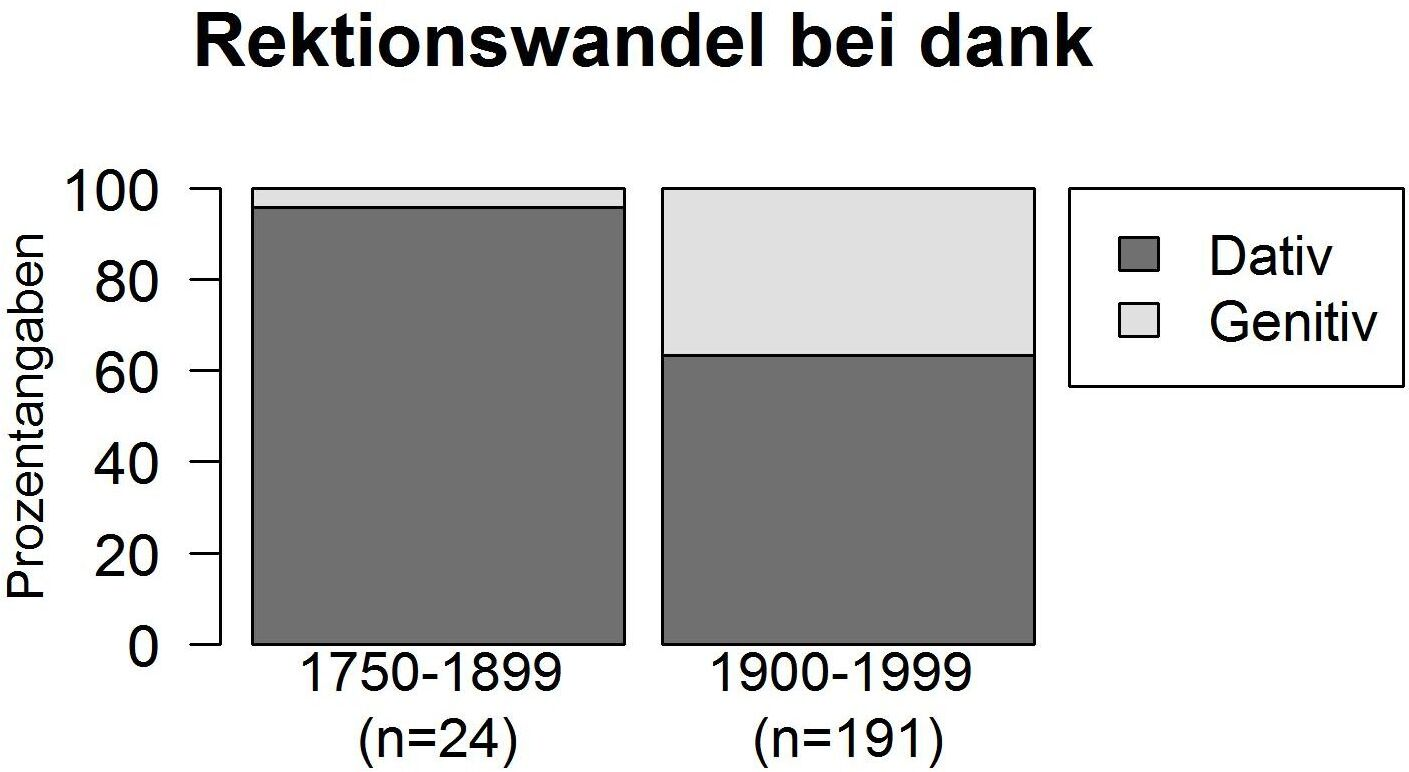
\includegraphics[scale=0.8]{Rektionswandeldank.jpg}
\caption{Kasusrektion von \object{dank} in Texten des DTA und des DWDS-Kernkorpus \citep[s.][]{Vieregge.2019}}
\label{pic:Rektionswandeldank}
\end{figure}

%Genitiv als Kasus denominaler Präpositionen
Diesen schnellen Übergang zur Genitivrektion erklärt \citet[25]{Agel1992} mit der Analogie zu semantisch ähnlichen Präpositionen wie \object{aufgrund} oder \object{infolge}. 
\citet[176]{DiMeola2004} weist jedoch darauf hin, dass Analogiebildungen keine hinreichende Erkl{\"a}rung bieten können, da sich für alle Fälle Gegenbeispiele finden lassen und unklar ist, warum einige Pr{\"a}positionen anf{\"a}llig sind, andere aber nicht. 
\citet[]{Eisenberg1979} sieht als Erklärung für die starke Tendenz von \dank{} zum Genitiv die Analogie zu anderen denominalen Präpositionen. 
Er versucht, eine klare Verteilung auszumachen, bei der die denominalen Pr{\"a}positionen zum Genitiv tendieren, die prim{\"a}ren Pr{\"a}positionen hingegen zum Dativ \citep[s.][519]{Eisenberg1979}. 
Allerdings lässt sich für die denominale Präposition \object{laut} im DTA und im DWDS-Kernkorpus beobachten, dass die Dativrektion vom 16. bis zum 20. Jahrhundert stetig ansteigt und schließlich ca. 90~\% ausmacht \citep[s.][]{Vieregge.2019}. 

Ein weiterer Punkt spricht sowohl dagegen, dass die Tendenz zum Genitiv am nominalen Spenderlexem liegt, als auch dagegen, dass es sich dabei um die Differenzierung von einem solchen Spenderlexem handelt: 
Bei den ursprünglichen Genitivpräpositionen \wegen{} und \waehrend{} ist kein Wechsel zum Dativ erkennbar, wie bereits der kurze diachrone Ausblick in \citet[]{DiMeola2000} angedeutet hat. 
Die Korpusuntersuchung im DTA und DWDS-Kernkorpus zeigt, dass die Entwicklung hin zum Prototyp bei der deverbalen Präposition \waehrend{} deutlich gehemmt ist, wie in \autoref{pic:Rektionswandelwaehrend} zu sehen \citep[s.][]{Vieregge.2019}.

\begin{figure}
\centering
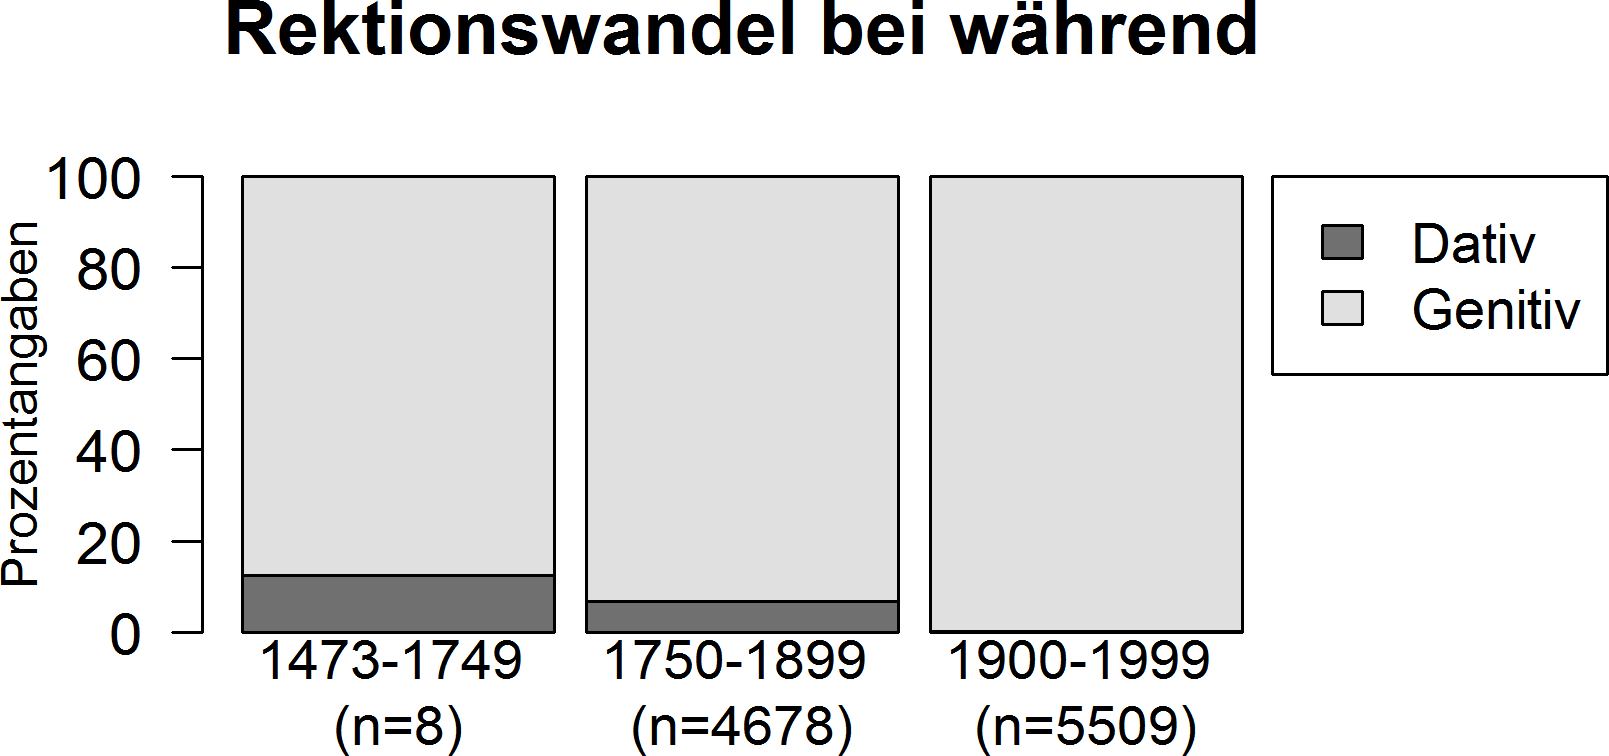
\includegraphics[scale=0.8]{Rektionswandelwaehrend.png}
\caption{Kasusrektion von \waehrend{} in Texten des DTA und des DWDS-Kernkorpus \citep[s.][]{Vieregge.2019}}
\label{pic:Rektionswandelwaehrend}
\end{figure}

\object{Während} wird im 18. Jahrhundert frequent. Von Beginn des Abdeckungszeitraums des DTA (1473) bis 1749 finden sich lediglich acht Belege für die Präposition, davon einer mit dem Dativ \citep[s.][]{Vieregge.2019}.
Zwischen 1750 und 1899 macht die Dativrektion 7~\% der Belege aus. 
Im 20. Jahrhundert hingegen weisen von 5509 Belegen lediglich 14 eine Dativrektion auf, d.\,h., in 99,7~\% der Fälle regiert die Präposition den Genitiv. 
Die Variation nimmt also deutlich zugunsten des Genitivs ab, eine Differenzierung von der Spenderstruktur erfolgt nicht. 

Ganz ähnliche Ergebnisse zur historischen Entwicklung der Rektion erhält \citet[]{Sato.2015}. 
Sie berücksichtigt die Präpositionen \wegen, \waehrend{} und \object{statt} in allen möglichen Stellungsvarianten mit Substantiven im Singular Maskulinum oder Neutrum in insgesamt 140 Gebrauchstexten von 1520 bis 1870 (je vier Texte pro Jahrzehnt) \citep[s.][30]{Sato.2015}. 
Die Studie zeigt eine Abnahme der Dativrektion bei \object{während} im 19. Jahrhundert \citep[s.][45--46]{Sato.2015}.
Für \wegen{}  stellt \citet[33]{Sato.2015} eine pl{\"o}tzliche Abnahme der Dativrektion ab 1800 fest: 
Der Dativ ist im 18. Jahrhundert signifikant h{\"a}ufiger als im 19. Jahrhundert, w{\"a}hrend f{\"u}r den Genitiv der umgekehrte Fall gilt~\citep[s.][34]{Sato.2015}.

%Produktionsexperiment Becker 2011
Dass sich die starke Tendenz zur Genitivrektion in der Gegenwartssprache fortsetzt, belegt ein Produktionsexperiment von \citet[]{Becker2011}. 
Sie legt 52 Studierenden zwei Lückentexte mit Sekundärpräpositionen vor, in denen jeweils die Flexionsendungen der Substantive und der Definitartikel in den Präpositionalphrasen ergänzt werden sollen \citep[s.][209]{Becker2011}. 
Die beiden Lückentexte unterscheiden sich laut \citet[209--210]{Becker2011} in der Formalität der gewählten Formulierungen. 
Da sich zwischen den beiden Lückentexten kaum Unterschiede ergaben, zeigt \autoref{table:Becker2011} eine Zusammenfassung aller Ergebnisse \citep[s.][210]{Becker2011}. 
\begin{table}
\centering
\begin{tabular}{lcc}
\lsptoprule
Laut kodifizierter Norm akzeptiert: & Anteil Genitivrektion & Anteil Dativrektion \\
\midrule
Nur Dativrektion \small{(\object{gemäß, außer, gegenüber, entsprechend, entgegen})}        & 65~\%                    & 35~\%                  \\
Dativ- und Genitivrektion \small{(\object{einschließlich, während, laut, innerhalb, dank})}  & 86~\%                    & 14~\%                  \\
Nur Genitivrektion  \small{(\object{bezüglich,ungeachtet, hinsichtlich, längs, jenseits})}  & 97~\%                    & 3~\%                   \\
\lspbottomrule
\end{tabular}
\caption{Zusammenfassung der Ergebnisse aus \citet[210]{Becker2011}}
\label{table:Becker2011}
\end{table}

Die Ergebnisse lassen eine eindeutige Präferenz für den Genitiv erkennen: 
{\glqq}Es wurde selbst dann der Genitiv bevorzugt, wenn es sich um eine -- laut den Grammatiken eindeutige~-- Dativpr{\"a}position handelte{\grqq}~\citep[211]{Becker2011}. 
Bei der Präposition \object{gegenüber}, die im Korpus \citeauthor{DiMeola2000}s (\citeyear{DiMeola2000}) kaum schwankt, verwendeten in \citeauthor{Becker2011}s Experiment 54~\% den Genitiv \citep[s.][211]{Becker2011}. 

Ebenfalls unerwartet vor dem Hintergrund der Differenzierungshypothese ist, dass sich in Korpora zumindest vereinzelt auch Belege für Primärpräpositionen mit dem Genitiv finden. 
\citet[259--260]{DiMeola2005b} etwa findet einige Belege für Primärpräpositionen mit Genitivrektion, bspw. für \object{seit} und \object{nach} \citep[s. auch][211]{DiMeola2009}. 
Auch \citeauthor{Vater.2009} (\citeyear[58]{Vater.2009} sowie \citeyear[220]{Vater.2015}) beobachtet den Genitiv bei der Prim{\"a}rpr{\"a}position \textit{seit}. 
Bei den Primärpräpositionen ist der Grammatikalisierungsprozess jedoch so weit vorangeschritten, dass das Differenzierungsprinzip nicht mehr greifen kann. 
Insgesamt scheint der Genitiv mit den meisten Präpositionen zumindest vereinzelt möglich zu sein. 
W{\"a}hrend bei den Beispielen, die \citeauthor{DiMeola2001} f{\"u}r ausschlie{\ss}liche Genitivpr{\"a}positionen anf{\"u}hrt, der Dativ tats{\"a}chlich nicht gebraucht wird (\textit{*diesseits dem Fluss, *zeit seinem Leben}), kommen etwa \object{fern} und \object{getreu}, die \citet[75--76]{DiMeola2001} als Beispiele f{\"u}r ausschlie{\ss}liche Dativpr{\"a}positionen anführt, im DWDS-Zeit-Korpus auch mit dem Genitiv vor. 
Für \object{getreu} finden sich lediglich vier, für \object{fern} jedoch ca. 70 Belege.
\citet[255]{DiMeola2005b} merkt außerdem an, dass von den urspr{\"u}nglichen Genitivpr{\"a}positionen bisher keine einzige vollst{\"a}ndig zum Dativ {\"u}bergegangen ist.
Der vollst{\"a}ndige {\"U}bergang von der Dativ- zur Genitivrektion l{\"a}sst sich hingegen laut \citeauthor{DiMeola2005b} (\citeyear[170]{DiMeola2004} sowie \citeyear[256]{DiMeola2005b}) bei \textit{trotz}, \textit{inmitten}, \textit{unfern }und \textit{unweit }beobachten. 

%\begin{quote}Der ungew{\"o}hnliche Vormarsch der Genitivrektion nach \textit{dank }zu Zeiten des allgemeinen Genitivr{\"u}ckgangs wird im Lichte des Determinativprinzips ebenfalls verst{\"a}ndlich. Da die Pr{\"a}postion auf eine Ellipse des Typs \textit{Dank [sei seinem Einflu{\ss} }zur{\"u}ckgeht (vgl. DU, S. 165), ist die urspr{\"u}ngliche Ausschlie{\ss}lichkeit der Dativrektion einleuchtend. Da jedoch die partiell synonymen Pr{\"a}positionen \textit{aufgrund, infolge, wegen }alle vom Determinativprinzip gesteuert werden, gesellt \textit{dank }sich langsam zu ihnen. \citep[25]{Agel1992}\end{quote}
%Analogie
%Zahlen aus dem DWDS.\footnote{Gesucht wurde mit Abfragen nach dem Muster "@dank @dem \#<2 \$p=NN".} \\
%\begin{table}
%\centering
%\label{RektionDWDS}
%\begin{tabular}{lcccc}
%\hline
 %                  & \multicolumn{2}{c}{1946-1981} & \multicolumn{2}{c}{1982-2016} \\
  %                 & Genitiv        & Dativ        & Genitiv        & Dativ        \\ \hline
%\textit{wegen}     & 99,0           & 1,0         & 99,5           & 0,5         \\
%\textit{während}   & 99,3           & 0,7         & 99,6           & 0,4         \\
%\textit{dank}      & 66,7           & 33,3         & 95,2           & 4,8         \\
%\textit{gegenüber} & 0           & 100         & 0,6           & 99,4        
%\\ \hline
%\end{tabular}
%\caption{Veränderung der Kasusrektion bei Sekundärpräpositionen}
%\end{table}
Die Daten zum Rektionswandel der Präpositionen zeigen deutlich, dass es eine starke Tendenz zum Genitiv gibt, während der Wechsel zur Dativrektion gebremst ist. 
Dies lässt sich mit dem Prototypisierungs- und dem Differenzierungsprinzip nicht ausreichend erklären. 
% Metapragmatik als Erklärungsfaktor
Offenbar ist die Entwicklung der Kasusrektion zusätzlich stark von der metapragmatischen Bewertung der Kasus beeinflusst. 
\citet[33--34]{Szczepaniak2014} etwa sieht die Aufladung mit sozialer Bedeutung und die Ideologie des Sprachverfalls als wesentliche Faktoren, die den Genitiv als Pr{\"a}positionalkasus f{\"o}rdern. 
\citet[36]{Lehmann1992} sprechen vom \glqq normativen Druck der Grammatiker\grqq{}, der den Genitiv begünstige. 
Ähnlich vermutet \citeauthor{Becker2011} als Grund für die starke Tendenz zum Genitiv in ihrem Produktionsexperiment, {\glqq}dass die Testpersonen mit dem Genitiv einen sozial markierten Sprachgebrauch verbinden und in der Testsituation ein entsprechendes Erwartungsmuster erf{\"u}llen wollten{\grqq}~\citep[211]{Becker2011}. 
\citet[218]{DiMeola2000} selbst misst der metapragmatischen Bewertung keine große Bedeutung bei. 
Er diskutiert ihren Einfluss unter dem Punkt {\glqq}Rolle der Standardisierung{\grqq} und kommt zu dem Schluss, dass hier {\glqq}Ursache und Wirkung verwechselt werden. Standardisierung hat n{\"a}mlich in erster Linie ratifizierenden, nicht propositiv-pr{\"a}skriptiven Charakter{\grqq} ~\citep[216]{DiMeola2000}. 
Dabei scheint er jedoch die komplexen Zusammenhänge zwischen Aussagen in Kodizes, laienlinguistischen Sprachideologien und dem Sprachgebrauch zu übersehen (\autoref{sec:MetapragmatikVariationWandel}). 
Auf diese wird im folgenden Kapitel eingegangen, das sich der Indexikalität der Präpositionalkasus als wesentlichem Faktor für die Variation und den Wandel der Präpositionen widmet. 
\section{Die Indexikalität der Rektionskasus} \label{sec:IndexikalitaetRektionskasus}
In den folgenden Abschnitten werden bisherige Studien vorgestellt, die auf die Registrierung und die Indexikalität der Rektionskasus hindeuten. 
Dabei soll zunächst auf Korpusstudien eingegangen werden, die einen Einblick in die Registrierung der Varianten geben (\autoref{sec:KorpusstudienRektion}). 
Anschließend wird in \autoref{sec:IndexikalitaetRektionskasushistorisch} dargestellt, inwiefern historische Grammatiken und sprachpflegerische Schriften zur Registrierung beigetragen haben.  
\autoref{sec:IndexikalitaetRektionskasusheute} geht auf Untersuchungen ein, die Hinweise darauf liefern, welche soziale Bedeutung die Präpositionalkasus heute für SprecherInnen des Deutschen haben. 
\subsection{Anhaltspunkte aus korpusbasierten Studien}
\label{sec:KorpusstudienRektion}
%Im von \citeauthor{Scott.2014} durchsuchten Zeitungskorpus GerManC, das Texte von 1650 bis 1800 enth{\"a}lt und insgesamt 100000 W{\"o}rter umfasst, kommt \textit{wegen} 68mal mit dem Genitiv und sechsmal mit dem Dativ vor, au{\ss}erdem zweimal mit dem Akkusativ. \textit{W{\"a}hrend }findet sich lediglich viermal, davon dreimal mit dem Genitiv~\citep[s.][243]{Scott.2014}. \\
Zwar zielen die bisherigen korpuslinguistischen Studien nicht darauf ab, explizite metapragmatische Äußerungen zur Registrierung der Rektionsvarianten zu erfassen, jedoch bieten Erkenntnisse zur Verteilung in Korpora implizite Hinweise darauf, welchen Registern eine Variante zugeordnet wird. 
Korpusstudien sind daher insbesondere für die \textit{presupposition}, also die Angemessenheit einer Variante im Kontext, aufschlussreich (\autoref{sec:Indexikalitaet}). 

\citet[]{DiMeola2000} untersucht in seiner Korpusstudie, wie sich die Rektionsvarianten auf verschiedene Textsorten verteilen. 
Dazu unterscheidet er zwischen folgenden fünf Textsorten: Pressesprache (Ausgaben der FAZ), Fachtexte (an ein Fachpublikum gerichtete rechts- und wirtschaftswissenschaftliche Texte), Sachprosa (Ratgeber und Reiseführer), Belletristik (Werke von 20 SchriftstellerInnen) und Unterhaltungsliteratur (von \citeauthor{DiMeola2000} näher angegeben als Kriminalromane und Frauenliteratur).\footnote{Unter Frauenliteratur fasst \citet{DiMeola2000} elf (Liebes-)Romane aus dem Unterhaltungsbereich, alle von weiblichen Verfasserinnen. Zu den Titeln gehören bspw. Dünnebier, Anna, \textit{Der Quotenmann} oder Luginger, Karin \textit{Männer fallen nicht vom Himmel}.} 
Die Genitivrektion bei ursprünglichen Dativpräpositionen kommt häufiger in nicht-fiktionalen Texten vor. 
So findet sich bspw. bei \dank{} in allen Textsorten häufiger die Genitivrektion, in Fach- und Pressetexten kommt sie aber ausschließlich vor \citep[s.][212]{DiMeola2000}. 
Die Dativrektion bei \textit{wegen }und \textit{w{\"a}hrend }kommt im Korpus \citeauthor{DiMeola2000}s hingegen insbesondere in Belletristik und Unterhaltungsliteratur vor \citep[s.][210]{DiMeola2000}. 
Der historisch neuere Dativ bei \textit{wegen }kommt 112-mal von 147-mal in fiktionalen Texten vor. 
Bei \waehrend{} kommt die Dativrektion in \citeauthor{DiMeola2000}s Korpus insgesamt lediglich zehnmal vor, davon achtmal in fiktionalen Texten. 
Hier zeigt sich also eine Ausdifferenzierung der Kasus nach Textsorten:~W{\"a}hrend die nicht-fiktionalen Texte zum Genitiv tendieren, wird in den fiktionalen Texten der Dativ bevorzugt.
Diese Textsortenaffinität kann auf die unterschiedliche Registrierung der Rektionsvarianten hindeuten. 
Eine solch starre Textsorteneinteilung wie sie bei \citet{DiMeola2000} und auch in vielen anderen Korpusuntersuchungen vorgenommen wird, ist allerdings problematisch, da bspw. nicht ersichtlich ist, in welchen Kontexten die Rektionsvarianten tatsächlich verwendet werden und welche Wirkung sie dort haben. 

Während die Texte im Korpus \citeauthor{DiMeola2000}s alle zur lektorierten Schriftlichkeit gehören, untersucht \citet[]{Elspa2005} private Briefe von EmigrantInnen aus dem 19. Jahrhundert. 
Er betrachtet unter anderem die Rektion der Präposition \wegen{} und findet 71 Belege, die eindeutig einem Kasus zugeordnet werden k{\"o}nnen. 
Davon weisen lediglich acht eine Genitivrektion auf, 45-mal wird der Dativ verwendet und 18-mal der Akkusativ~\citep[s.][321]{Elspa2005}.\footnote{Die Akkusativrektion erklärt \citet[]{Elspa2005} mit dem Einfluss von Dialekten, in denen Akkusativ und Dativ häufig zusammenfallen.}
Insbesondere unge{\"u}bte SchreiberInnen verwenden den Dativ oder den Akkusativ, in den Briefen routinierter SchreiberInnen hingegen findet sich in vier von sechs Fällen der Genitiv \citep[s.][321--323]{Elspa2005}. 
Ein diachroner Vergleich zeigt, dass der Dativ in den Briefen vom 17. bis zum 19. Jahrhundert h{\"a}ufiger wird, sodass im 19. Jahrhundert in der informellen Schriftlichkeit die Dativrektion {\"u}berwiegt~\citep[s.][411]{Elspa.2015}. 
In Texten aus dem Zeitungskorpus des GerManC und dem Kaiserreich-Corpus (KuK-Corpus), die zusammen den Zeitraum 1650 bis 1918 abdecken, wird \wegen{} hingegen {\"u}berwiegend mit dem Genitiv gebraucht~\citep[s.][410]{Elspa.2015}. 
\citeauthor{Elspa2005} schlie{\ss}t aus der Verteilung der Rektion, \begin{quote}dass der Gebrauch von Pr{\"a}positionen, die den Genitiv regieren sollen, im 19. Jahrhundert nicht in der Alltagssprache verwurzelt, sondern ein Merkmal gebildeter Schreibender war.~\citep[321]{Elspa2005}\end{quote}
\citet[]{Sato.2015} nimmt in einer stärker qualitativ ausgerichteten Untersuchung die Kasuswahl nach \wegen{}, \waehrend{} und \object{statt} in verschiedenen Schriften Beethovens in den Blick.  Sie betrachtet zum einen die Konversationshefte, durch die der am Ende seines Lebens mehr und mehr gehörlose Beethoven mit Angehörigen und Bekannten kommunizierte, zum anderen aber auch Briefe und eine theoretische Schrift. 
Zwar zeigt sich eine eindeutige Verteilung, da in der theoretischen Abhandlung ausschließlich der Genitiv gebraucht wird, in den sehr informellen Konversationsheften dagegen fast ausschließlich der Dativ \citep[s.][27]{Sato.2015}. 
Die Belegzahlen sind allerdings sehr gering (zwischen fünf und 130 Belege pro Textsorte) und es handelt sich um einen einzigen Schreiber. 
Da zwischen einzelnen SchreiberInnen immer individuelle Unterschiede zu erwarten sind, ist dies für eine variationslinguistische Untersuchung nicht optimal. 
Interessant ist aber der Blick auf die Kasuswahl mit verschiedenen KommunikationspartnerInnen. 
Beethovens Neffe Karl wählt in der Kommunikation mit seinem Onkel, zu dem er kein gutes Verhältnis hatte, häufiger den Genitiv als mit anderen KommunikationspartnerInnen, was \citet[s.][29]{Sato.2015} als Mittel deutet, Distanz zu evozieren. 
% Änderung Anfang 
In \citet{Sato.2022} werden neben Beethovens Briefen und Konversationsheften private Briefe von Haydn, Bach, Goethe und der Familie Mozart berücksichtigt.
Die Auswertung der Briefe von Mitgliedern der Familie Mozart zeigt bspw., dass die Genitivrektion bei \wegen{} in Briefen an Familienangehörige signifikant seltener ist als in Briefen an Personen, die nicht zur Familie gehören \citep[s.][96--97]{Sato.2022}. 

In einer Untersuchung von \wegen{} in 39 zwischen 1750 und 1850 erschienenen Dramen zeigt \citet[]{Sato.2016} außerdem, dass Dramenfiguren aus oberen Schichten bei dieser Präposition h{\"a}ufiger der Genitiv in den Mund gelegt wird, Figuren aus unteren Schichten dagegen der Dativ~\citep[s.][409]{Sato.2016}: 
54 von 59 Vorkommen von \wegen{} mit Genitivrektion lassen sich Figuren der oberen Schichten zuordnen, 17 von 20 Vorkommen mit Dativrektion hingegen Figuren aus unteren Schichten.

% gesprochene Sprache 
Die Kasuswahl in gesprochener Sprache untersucht \citet[]{Petig1997}. 
Er wertet zwei Korpora (das Pfeffer-Korpus von 1961 und das Jones-Korpus von 1992) mit insgesamt 800 ca. zehnminütigen Interviews zu verschiedenen Themen aus~\citep[s.][36]{Petig1997}.\footnote{Zu den Themen schreiben \citet[17]{Pfeffer.1984}, dass zwar zunächst jeweils eines von 25 zuvor bestimmten Themen, wie etwa Wetter, Schule und Erziehung oder Freizeit, vorgegeben war, die GesprächspartnerInnen von diesem aber häufig abwichen, wodurch \glqq die Natürlichkeit und Ungezwungenheit erhöht\grqq{} worden sei.} 
Unter den SprecherInnen des Korpus finden sich je ca. 200 Frauen und Männer aller Alters- und Bildungsgruppen aus verschiedenen Regionen in Deutschland, {\"O}sterreich und der Schweiz \citep[s.][17]{Pfeffer.1984}. 
\citeauthor{Petig1997} betrachtet die Präpositionen \object{während}, \object{wegen}, \object{(an)statt} und \object{trotz} mit Maskulina oder Neutra im Singular und Plural. 
\object{(An)statt} und \object{trotz} kommen nur selten vor, \wegen{} und \waehrend{} sind deutlich frequenter. 
Sie treten in den Interviews allerdings beide nur sehr selten mit dem Dativ auf~\citep[s.][37]{Petig1997}: 
Lediglich zwischen 4~\% (\waehrend{} im Pfeffer-Korpus) und 11~\% (\wegen{} im Jones-Korpus) der Belege entfallen auf die Dativrektion \citep[s.][37]{Petig1997}. 
Die wenigen Belege mit der Dativrektion finden sich insbesondere in s{\"u}ddeutschen Dialekten~\citep[s.][38]{Petig1997}. 
Dieser Befund deutet scheinbar darauf hin, dass die Genitivrektion in der gesprochenen Sprache die deutlich häufigere Variante ist. 
Ob dies jedoch auf natürliche Interaktionssituationen übertragbar ist, ist fraglich. 
\citet[37]{Petig1997} selbst weist darauf hin, \glqq that people may speak more formally in an interview situation when they know they are being recorded.\grqq{}

Die regionale Verteilung der Rektionsvarianten betrachtet auch \citet{Elter2005}. 
Anhand einer Untersuchung der Pr{\"a}positionen \wegen, \waehrend, \dank, \object{trotz} und \object{statt} mit Definitartikel im Maskulinum oder Neutrum in Zeitungen aus Deutschland, Österreich und der Schweiz zeigt sie, dass es in der Zeitungssprache insgesamt wenige Belege mit Dativ gibt \citep[s.][128]{Elter2005}. 
\textit{Wegen} regiert in 0,8~\% der Belege den Dativ, \waehrend{} in 0,3~\%, \dank{} in 7~\% \citep[s.][128]{Elter2005}. 
Dabei lassen sich regionale Unterschiede beobachten. 
So regiert \dank{} in schweizerdeutschen Zeitungen weitaus h{\"a}ufiger den Dativ~\citep[s.][134]{Elter2005}. 
Bei \waehrend{} entfallen fast alle Belege für die Dativrektion auf die Schweiz, bei \wegen{} ist die Verteilung hingegen weniger deutlich \citep[s.][130--131]{Elter2005}.
Die Dativrektion könnte von SprachbenutzerInnen potenziell also als indexikalischer Verweis auf schweizerdeutschen Sprachgebrauch gedeutet werden. 
In \citeauthor{Elter2005}s Untersuchung deutet sich außerdem an, dass der Dativ als Pr{\"a}positionalkasus bei Sekund{\"a}rpr{\"a}positionen offenbar verwendet wird, um Umgangssprache bzw. m{\"u}ndlichen Sprachgebrauch zu evozieren, wie etwa in diesem Beispiel \citep[s.][128--129]{Elter2005}:
\begin{exe}
\ex \object{Die anderen Bandmitglieder haben {\glq}Number Nine{\grq} wegen ihres fortgeschrittenen Alters verlassen... {\glq}Wir spielen, was die Leute h{\"o}ren wollen{\grq}, erkl{\"a}rt Frank das Song-Repertoire, setzt allerdings gleich hinzu:~{\glq}Aber nicht alles! Die  {\glq}B{\"o}hsen Onkelz{\grq} haben wir nie performed, wegen dem Nazi-Image.{\grq}} (Nordbayrische Nachrichten, 14.12.2002, Beispiel aus \citealp[129]{Elter2005})
\end{exe}
Gerade für \wegen{} stellt \citet[128]{Elter2005} fest, dass die Dativrektion häufig in wörtlichen Zitaten auftritt. 
Diese Verteilung spricht für eine Registrierung des Dativs als mündlichkeitsnah.

Die Registrierung des Dativs als informell und des Genitivs als formell wird durch verschiedene weitere Faktoren gestützt. 
Ein Faktor besteht darin, dass es in den Dialekten des Deutschen so gut wie keinen Genitiv gibt (\citealp[s.][437]{Shrier.1965}; \citealp[250]{Scott.2014}). Lediglich in einigen wenigen Dialekten werden noch Genitive gebraucht, bspw. in der schweizer Region Wallis \citep[s.][1243]{Ko.1983}.\footnote{\citet[339]{Scott.2014} weist darauf hin, dass empirische Untersuchungen dazu, welche Formen und Funktionen des Genitivs in Dialekten des Deutschen überhaupt vorhanden sind, noch ausstehen. Für das Luxemburgische zeigt \citet{Dohmer.2018}, dass Genitive vorhanden, aber nur eingeschränkt produktiv sind. \citet{Hoge.2018} argumentiert, dass das Jiddische einen possessiven Genitiv aufweise.} 
Da Dialekte in der Vorstellung der SprachbenutzerInnen für eher informelle, private kommunikative Praktiken genutzt werden, begünstigt dies die Wahrnehmung des Dativs als informell~\citep[s.][221--222]{Maitz2015}. 
Hinzu kommt, dass der Genitiv nicht nur als Präpositionalkasus, sondern auch als Attribut- und Objektkasus eher in formellen Registern zu verorten ist, wie \citet[252]{Scott.2014} anhand eines Vergleichs von Spiegel-Artikeln mit dem Dortmunder Chat-Korpus sowie gesprochener Sprache aus dem Wende-Korpus zeigt. 
Als Grund daf{\"u}r, dass der Genitiv in informellen Registern seltener ist, sieht \citet[s.][276]{Scott.2014} jedoch nicht eine Vermeidung des Kasus, sondern vielmehr, dass Strukturen, in denen ein Genitiv als Variante m{\"o}glich w{\"a}re, insgesamt seltener sind: 
\glqq the connection of two noun phrases in a broadly possessive relationship and the use of genitive-assigning prepositions is simply rare in informal language use\grqq{}~\citep[276]{Scott.2014}.

%Registrierung Sekundärpräpositionen
Ein weiterer Faktor, der die Registrierung der Rektionskasus stützt, ist die Registrierung der Sekundärpräpositionen selbst als formell und schriftsprachlich. 
Zwar kommen sie auch in gesprochener Sprache vor, wie eine Untersuchung von \citet[]{Mikosch1987} zeigt, die auf Transkriptionen süddeutscher dialektaler Gesprächsdaten aus den 50er Jahren basiert. 
Bis auf \wegen{} sind sie hier jedoch nur selten vertreten; \dank{} findet sich in den Daten \citeauthor{Mikosch1987}s (\citeyear[125]{Mikosch1987}) bspw. überhaupt nicht.
\citet[48]{Bene.1975} sch{\"a}tzt, dass die sehr wenig prototypischen Pr{\"a}positionen vor allem in Wissenschafts- und Sachregistern angesiedelt sind. 

Im Rahmen der oben bereits beschriebenen Korpusuntersuchung im DWDS-Kernkorpus \citep[s.][]{Vieregge.2019} wurde die Verteilung von \waehrend, \dank, \object{laut} und \object{entsprechend} auf die dort angelegten Textsorten \glqq Zeitung\grqq, \glqq Wissenschaftssprache\grqq, \glqq Gebrauchsliteratur\grqq{} und \glqq Belletristik\grqq{} untersucht. 
\autoref{pic:TextsortenDWDS} zeigt die Verteilung der Treffer für die gesuchten Präpositionen plus \object{dem} oder \object{des} im Vergleich zur Verteilung aller Tokens im Korpus.
\begin{figure}
\centering
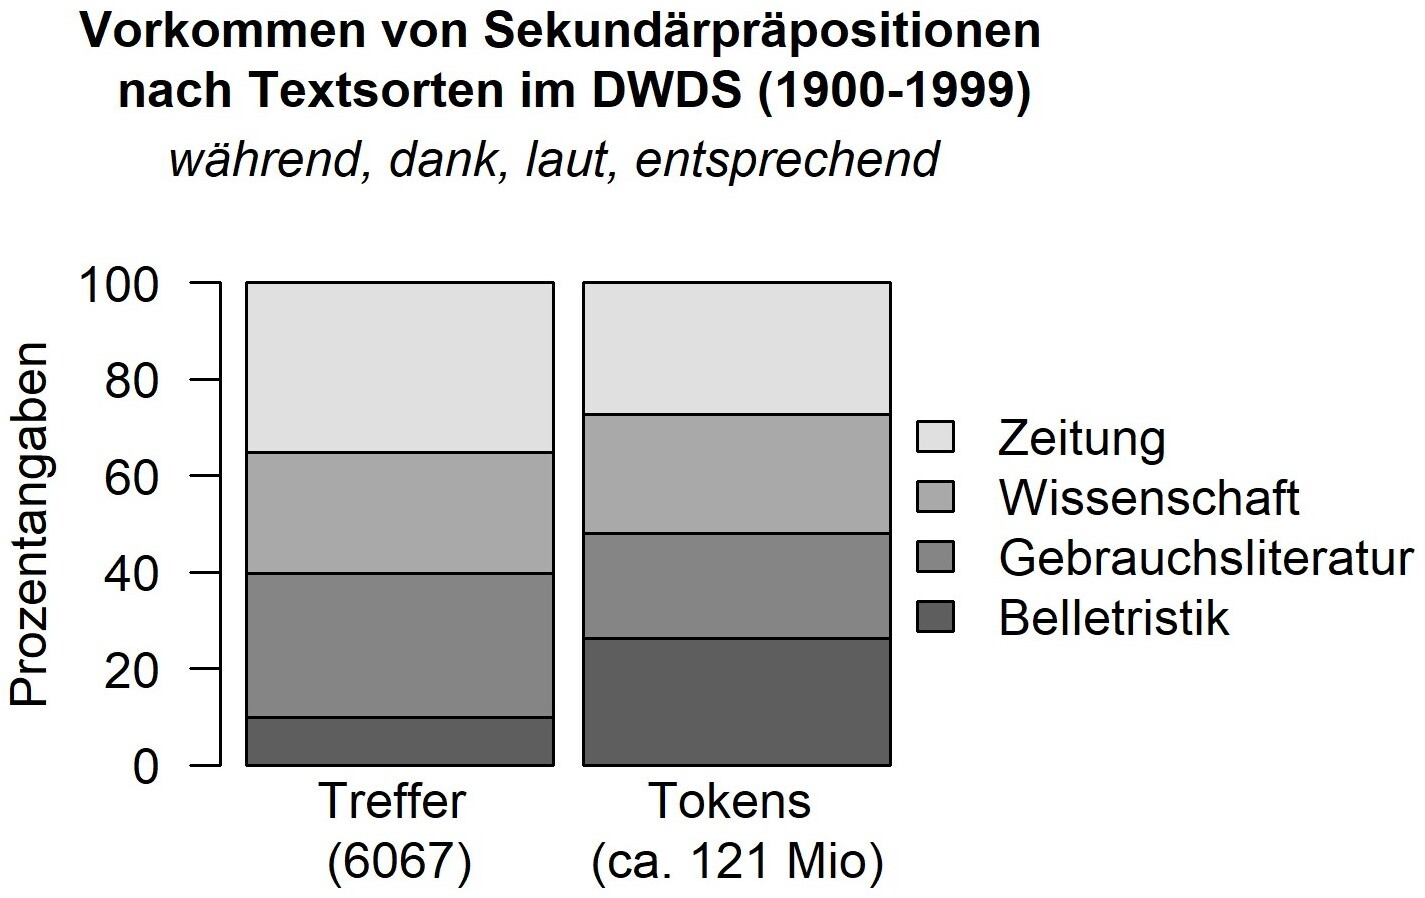
\includegraphics[scale=0.9]{TextsortenDWDS.jpg}
\caption{Textsortenverteilung von \waehrend, \dank, \object{laut} und \object{entsprechend} \citep[s.][]{Vieregge.2019}}
\label{pic:TextsortenDWDS}
\end{figure}

Bis auf den Bereich Wissenschaftssprache lässt sich keine dieser Textsorten pauschal als formelles oder informelles Register bezeichnen. 
Dennoch ist es interessant, mit welchen Textsorten der Gebrauch dieser Sekundärpräpositionen verknüpft ist. 
Wie man sehen kann, ist die Verteilung der untersuchten Sekundärpräpositionen anders als die aller Tokens im Korpus. 
Die gesuchten Konstruktionen zeigen eine leichte Affinität zur Zeitungssprache sowie zu Gebrauchstexten. 
In der Belletristik kommen die Sekundärpräpositionen hingegen seltener vor, in der Wissenschaftssprache zeigt sich kein Unterschied zur Verteilung aller Tokens \citep[s.][]{Vieregge.2019}. 
Ein Chi-Quadrat-Test zeigt, dass der Unterschied zwischen der Textsortenverteilung der gesuchten Sekundärpräpositionen und der aller Tokens signifikant ist, aber nur eine geringe Effektstärke aufweist ($\chi$=30,7; p<0,001; Cramer's V=0,071).
In der Tendenz kommen Sekundärpräpositionen also vor allem in informationsorientierten Texten vor.

\citet[176--184]{DiMeola2000} überprüft bei seiner Korpusuntersuchung die Textsortenverteilung für einzelne Präpositionen. 
Für \waehrend{} stellt er fest, dass die Präposition am häufigsten in Sachtexten vertreten ist.
\object{Wegen} und \dank{} kommen hingegen insbesondere in Pressetexten vor und \gegenueber{} in fachsprachlichen Texten. 
Insgesamt kommt \citet[184]{DiMeola2000} zu dem Schluss, dass Sekundärpräpositionen typisch für fachsprachliche Texte seien, während Primärpräpositionen keine textsortenspezifische Verteilung zeigten. 
Die Genitivrektion wird also auch deswegen als formell registriert, weil die Sekund{\"a}rpr{\"a}positionen, von denen die meisten den Genitiv regieren, vor allem in formellen Registern vorkommen~\citep[s.][209]{Becker2011}. 

Zusammenfassend lässt sich festhalten, dass korpusbasierte Studien bereits einige Anhaltspunkte zur Registrierung der Rektionskasus von Sekundärpräpositionen bieten. 
Bei \citet[]{DiMeola2000} zeigt sich, dass die Dativrektion insgesamt selten ist und dabei in fiktionalen Texten häufiger vorkommt als in nicht-fiktionalen. 
In der privaten Schriftlichkeit des 19. Jahrhunderts nutzen geübte SchreiberInnen die Genitivrektion eher als ungeübte SchreiberInnen \citep[s.][]{Elspa.2005}. 
Dies deutet auf eine frühe Assoziation des Kasus mit Bildung und dadurch auch mit der Standardsprache als Varietät der Bildungsschicht hin. 
In historischen Zeitungstexten findet sich vorwiegend die Genitivrektion \citep[s.][]{Elspa.2015}. 
Während der Genitiv also verstärkt in Registern des öffentlichen Sprachgebrauchs auftritt, lässt sich der Dativ im Privaten verorten. 
Dies bestätigen qualitative Untersuchungen von \citeauthor{Sato.2015} (\citeyear{Sato.2015} und \citeyear{Sato.2016}) zum Sprachgebrauch Beethovens und zu Dramentexten. 
In den von \citet{Petig1997} untersuchten gesprochensprachlichen Korpora finden sich erstaunlich wenige Fälle von Dativrektion.
Sollte dies ein Effekt sozialer Erwünschtheit sein, so wäre auch dies ein Hinweis auf die Indexikalitäten der Kasus: 
\citet[37]{Petig1997} vermutet, die InterviewpartnerInnen gingen davon aus, mit der Verwendung der Genitivrektion einen besseren Eindruck zu hinterlassen.
Ob es für diese Vermutung konkrete Anhaltspunkte in den Interviews gibt, bleibt allerdings unklar. 
Auf eine mögliche Registrierung als regionalspezifisch deutet die Untersuchung zu Zeitungstexten von \citet{Elter2005} hin, in der die Dativrektion v.\,a. in der Schweiz vorkommt. 
\subsection{Registrierung durch Grammatiken und sprachpflegerische Schriften} \label{sec:IndexikalitaetRektionskasushistorisch}
Für die Registrierung als sprachideologischen Prozess ist nicht nur die Verteilung in Korpora relevant, sondern insbesondere der metapragmatische Diskurs. 
Dieser wird im Folgenden zunächst anhand von Analysen historischer Grammatiken und sprachpflegerischer Schriften beleuchtet. 

% Historische Grammatiken 
\citet{Davies2006} untersuchen Sprachurteile in Grammatiken und sprachpflegerischen Schriften von 1600 bis 2005.
Für \wegen{} stellen sie fest, dass die Präposition im 17. Jahrhundert zwar sowohl als Dativ- als auch als Genitivpr{\"a}position beschrieben wird, die Toleranz der Grammatiker von da an aber abnimmt~\citep[s.][202]{Davies2006}.
Die erste Erwähnung von \wegen{} findet sich 1641 in Gueintz' Sprachlehre, hier wird als Rektionskasus nur der Dativ genannt~\citep[s.][209]{Davies2006}. 
Die erste Stigmatisierung der Dativrektion findet sich dann bereits bei \citet[245]{Heynatz.1777}: 
\glqq Es ist unrichtig, wenn man \object{anstatt}, \object{längst}, \object{während} und \wegen{} anstatt des Genitivs mit dem Dativ setzt.\grqq
Noch negativer äußert sich \citet[]{Matthias.1929} in seinem erstmals 1892 erschienenen Werk \glqq Sprachleben und Sprachschäden\grqq:
\begin{quote} Durchaus gebührt \object{ohne} der vierte Fall: \object{ohne dich, ohne das Kind}, und \wegen{} der zweite: \object{wegen des Vergehens} oder \object{des Vergehens wegen}. […] [D]agegen hüte man sich, die volksmäßige Verunstaltung: \object{mit jemand von wegen einem Vorkommnisse reden müssen} u.\,ä. nachzuahmen. \citep[141]{Matthias.1929} \end{quote}
Der Dativ wird also explizit abgewertet und mit Volkstümlichkeit in Verbindung gebracht. 
Dass die Dativrektion in manchen Fällen auch in der formellen Schriftlichkeit akzeptiert wird (etwa bei artikellosen Substantiven im Plural), findet bis in die 1980er Jahre kaum Erwähnung und wird somit ausgeblendet \citep[s.][205, 209]{Davies2006}. 
Die Studie von \citet[]{Davies2006} zeigt, dass die Registrierung des Genitivs als Prestigekasus und die Stigmatisierung des Dativs Prozesse sind, die sich seit dem 18. Jahrhundert bis heute fortsetzen. 
Zusammenfassend konstatieren \citeauthor{Davies2006}:\begin{quote}The genitive case is considered to be a proud and important case of German grammar and any developments in favour of other cases are frowned upon and should be fought. \citep[209]{Davies2006}\end{quote}
% Grammatiken heute
Heute wird sowohl in der Sprachwissenschaft als auch von Grammatiken und im laienlinguistischen Diskurs immer darauf hingewiesen, die Variation zwischen Genitiv- und Dativrektion orientiere sich im Wesentlichen am Register (\citealp[s. etwa][172]{Barbour1998}; \citealp[135]{Elter2005}; \citealp[182]{Eisenberg.2013}).  
Der \citeauthor{Duden2016} gibt an: \begin{quote}Prinzipiell hat man bei der Kasuswahl Freiheit, sieht man von Stilunterschieden ab. Der Genitiv gilt als eher schriftsprachlich und stilistisch h{\"o}her stehend.~\citep[{\S}910]{Duden2016}\end{quote}
Ältere Dudenausgaben allerdings führen \wegen{} ausschlie{\ss}lich unter dem Eintrag zu den Genitivpr{\"a}positionen auf \citep[s.][208]{Davies2006}. 
\citet[358]{Helbig.2017} bezeichnen die Dativrektion bei \textit{wegen }und \textit{w{\"a}hrend }sowie bei anderen urspr{\"u}nglichen Genitivpr{\"a}positionen als \glqq umgangssprachlich\grqq, wird sie nicht als Ersatz f{\"u}r einen nicht erkennbaren Genitiv im Plural gebraucht. 
Die Genitivrektion bei urspr{\"u}nglichen Dativpr{\"a}positionen wie \textit{dank }oder \textit{zufolge }hingegen wird nicht als umgangssprachlich bezeichnet, sondern lediglich als Variante neben der Dativrektion aufgef{\"u}hrt~\citep[s.][358]{Helbig.2017}. 
Damit wird der Wandel zur Dativrektion implizit gegenüber dem Wandel zur Genitivrektion abgewertet. 

%Bastian Sick
Besondere Prominenz haben die sprachpflegerischen Kolumnensammlungen Bastian \citeauthor{Sick2006}s erhalten, deren Titel \textit{Der Dativ ist dem Genitiv sein Tod} zu einem Topos im Diskurs um den Genitiv geworden ist. 
Zu \wegen{} liest man dort etwa: 
\begin{quote} Welch wohlklingende Wortwahl: wegen des Winterwetters! Und dagegen nun der schnöde Dativ: wegen dem Winterwetter. Was klingt besser? \citep[101]{Sick2006} \end{quote}
Die Funktion der bewusst unterhaltsam geschriebenen Texte besteht insbesondere in der Abgrenzung gegenüber Gruppen, denen der Gebrauch der Dativrektion und anderer stigmatisierter sprachlicher Formen zugeschrieben wird.  
\citeauthor{Sick2006} und seinem Wirken wird eine wichtige Rolle bei der Verbreitung der Ideologie vom Aussterben des Genitivs zugesprochen: 
\begin{quote}Although the idea that the genitive case is in mortal danger (particularly as a result of encroachment from the dative)~is not new, Sick has certainly contributed greatly to the perception of a genitive under threat, and his title has entered the popular consciousness.~\citep[24]{Scott.2014}\end{quote}
\citet[323]{Langer.} verweist daneben aber auch auf Medien wie Die Zeit, den Spiegel und die S{\"u}ddeutsche Zeitung sowie den Sprachpfleger Wolf Schneider, die in Artikeln den Verlust des Genitivs und damit einhergehend eine {\glqq}Verarmung geistiger Ausdruckskraft{\grqq} beklagten. 
\citet[9]{Krause2012b} stellt die aus ihrer Sicht hyperkorrekte Verwendung des Genitivs in einen direkten Zusammenhang mit popul{\"a}rwissenschaftlichen Werken wie denen \citeauthor{Sick2006}s. 
In einer Untersuchung des Rektionsverhaltens von \object{entlang} kann sie allerdings keinen zeitlichen Zusammenhang zwischen einer Zunahme der Genitivrektion und dem Erscheinen von \citeauthor{Sick2006}s Schriften feststellen \citep[s.][347]{Krause2012a}. 
Dennoch betrachtet sie, ähnlich wie \citet[211]{Becker2011} die Indexikalität der Genitivrektion als Grund für ihre hohe Frequenz: 
Als Motivation, den Genitiv zu w{\"a}hlen, sieht \citet[19]{Krause2012b}, {\glqq}dass im Zweifelsfall der Genitiv das Elegantere, Rettenswerte, Vornehmere ist{\grqq}. 

% Stigmatisierung hyperkorrekter Genitiv
\citeauthor[]{Scott.2014} weist darauf hin, dass auch der Gebrauch des Genitivs mit urspr{\"u}nglichen Dativpr{\"a}positionen bereits seit Jahrhunderten stigmatisiert wird: \glqq Frequently, this use of the genitive is objected to by those who otherwise decry the replacement of the genitive\grqq{} \citep[303]{Scott.2014}.
Dies lässt sich z.\,T. auch noch in neueren Grammatiken beobachten. 
\citet[374]{Jung1980} schreibt zu \textit{dank }:\textit{~}{\glqq}\textit{dank }fordert den Dativ (der Genitiv ist weniger gut){\grqq}.
Ebenso macht \citeauthor{Sick2006} sich über den \glqq hyperkorrekten\grqq{} Gebrauch des Genitivs bei Präpositionen wie \object{trotz} lustig \citep[s.][210]{Davies2006}. 
F{\"u}r \dank{} mit Genitivrektion l{\"a}sst sich in den Grammatiken allerdings eine sehr rasche Verbreitung im Vergleich zu \wegen{} mit Dativ feststellen~\citep[s.][257]{Baumann2014}. 
Auch dies kommt einer impliziten Bevorzugung des Genitivs gleich. 

% Baumann/Dabóczi, Schulen
Neben Grammatiken und sprachpflegerischen Schriften zählt auch die Schule zu den Sprachautoritäten, die den Diskurs um die Rektionskasus prägen. 
\citet{Baumann2014} führen eine Umfrage unter angehenden und praktizierenden LehrerInnen durch, in der sie unter anderem nach der Akzeptabilität von \wegen{} und \dank{} mit der Dativrektion in Schülertexten fragen. 
Obwohl der Duden zum Zeitpunkt der Befragung jeweils beide Rektionsvarianten als korrekt angibt, wird die Dativrektion bei beiden Präpositionen nur von ca. der Hälfte der 92 Befragten akzeptiert \citep[s.][264--265]{Baumann2014}. 
Dies deutet darauf hin, dass die Dativrektion von vielen nicht als Teil des Standardsprachrepertoires gesehen wird. 

Der Blick in historische Grammatiken und sprachpflegerische Schriften offenbart lange andauernde Registrierungs- und Indexikalisierungsprozesse. 
Es kommt bereits früh zu einer sowohl impliziten als auch expliziten Stigmatisierung der Dativrektion \citep[s.][]{Davies2006}. 
An dieser wirken nicht nur Grammatiken des 18. bis 19. Jahrhunderts und sprachpflegerische Schriften mit, sondern ebenso der Duden, linguistische Veröffentlichungen sowie die Schule (vgl. \autoref{sec:Prestigevarietaet}). 
\subsection{Indexikalität der Rektionskasus im laienlinguistischen Diskurs} \label{sec:IndexikalitaetRektionskasusheute}
Eine wesentliche Rolle für die unterschiedliche Bewertung der Genitiv- und der Dativrektion spielt der laienlinguistische Diskurs in weniger institutionalisierten Bereichen, also im Alltag der SprachbenutzerInnen. 
Dieser Art laienlinguistischer Sprachurteile widmet sich die vorliegende Studie in besonderem Maße. 
Dieser Bereich ist besonders relevant, da sich hier zeigt, welche Ideologien und Einstellungen aus dem stärker institutionalisierten Bereich des Diskurses in das geteilte Wissen der SprachbenutzerInnen aufgenommen worden sind. 
Bisher wurde dies kaum empirisch untersucht. 
Die Einblicke, die die wenigen vorhandenen Untersuchungen bieten, werden im Folgenden vorgestellt. 

%Renata, Foren
\citet[]{Szczepaniak2014} betrachtet laienlinguistische Forenbeiträge, in denen über die Rektion von Sekundärpräpositionen diskutiert wird und kommt zu dem Schluss:
\glqq Die Rektionsschwankung bei \wegen{} ist im laienlinguistischen Bewusstsein fest etabliert. Dabei ist der Dativ auch heute noch negativ konnotiert\grqq{} \citep[45]{Szczepaniak2014}.  
SprachbenutzerInnen sehen die Kasusschwankungen h{\"a}ufig als gleichwertig mit einem Abbau des Genitivs~\citep[s.][45]{Szczepaniak2014}. 
Die Tendenz zum Genitiv wird dabei ausgeblendet: Aufgrund der hohen soziolinguistischen Salienz von \textit{wegen }wird davon ausgegangen, dass es dem Genitiv lediglich in Einzelf{\"a}llen gel{\"a}nge, den Dativ zur{\"u}ckzudr{\"a}ngen~\citep[s.][45, 46]{Szczepaniak2014}.
Offenbar haben SprachbenutzerInnen den Eindruck, dass ausgerechnet die als besser empfundene Variante seltener ist, und kommen daher zu dem Schluss, die Sprache verfalle~\citep[s.][36]{Szczepaniak2014}. 

% Masterarbeit, Foren
In \citet[]{Vieregge.2015} werden Kommentare in Onlineforen zu den Präpositionen \textit{ähnlich}, \textit{anstatt}, \textit{dank}, \textit{gegenüber}, \textit{kraft}, \textit{trotz}, \textit{während} und \textit{wegen} untersucht. 
Dafür wurde ein Gesamtkorpus aus 20 Diskussionsverläufen mit insgesamt 353 Beträgen aus verschiedenen Foren erstellt. 
Hier zeigt sich, dass neben der Ideologie des Sprachverfalls auch die Standardsprachideologie einen starken Einfluss hat \citep[s.][]{Vieregge.2015}. 
Diese äußert sich zum einen in Fragen der ForenuserInnen nach der richtigen Variante, zum anderen in den Antworten, die ein präskriptives Urteil fällen, nur eine Variante als richtig darstellen und Variation damit von vornherein ausblenden. 
Die Auffassung, es gebe eine richtige und eine falsche Variante, ist in ca. 40~\% der Aussagen des Korpus vertreten.
Dabei wird die Dativrektion 31-mal als falsch bezeichnet, die Genitivrektion hingegen nur 15-mal, also ungefähr halb so oft. 
Nur sehr wenige DiskursteilnehmerInnen gehen bei den Rektionsschwankungen von gleichwertigen Varianten aus.
Diachroner Wandel wird als Grund für Variation zwar in Betracht gezogen, allerdings häufig negativ bewertet. 
Die Vorstellung von einem drohenden oder gerade stattfindenden Sprachverfall ist relativ verbreitet, was unter anderem die zahlreichen Kommentare nach dem Muster \object{der Dativ ist dem Genitiv sein Tod} zeigen, die auf die Bücher \citeauthor{Sick2006}s verweisen.
Variation wird in den Foren also selten positiv gesehen. 
Sie stellt für viele SprecherInnen offenbar vor allem ein Anzeichen von Inkompetenz (entweder eigener oder fremder) oder Sprachverfall dar. 
Der Dativ wird außerdem mit niedrigem sozialen Status, Mündlichkeit und Umgangssprache in Verbindung gebracht: 
\begin{exe}
\ex \object{Den Dativ kannst du allenfalls in der mündlichen Sprache unter Nichtakademikern verwenden.} (https://www.gutefrage.net/frage/wegen-dem-hund-oder-des-hundes-wegen-oder, zuletzt aufgerufen am 13.09.2020)
%https://www.gutefrage.net/frage/wegen-dem-hund-oder-des-hundes-wegen-oder
\label{BspNichtakademiker}
\ex \object{Schon in einem Grammatikbuch aus den fünfziger Jahren stand: Wer} wegen \object{mit dem Dativ gebraucht, spricht ungepflegt.} (https://www.gutefrage.net/frage/wegen-dem-hund-oder-des-hundes-wegen-oder, zuletzt aufgerufen am 13.09.2020) 
\label{BspGrammatikbuch50er}
%https://www.gutefrage.net/frage/wegen-dem-hund-oder-des-hundes-wegen-oder
\end{exe}
In \autoref{BspNichtakademiker} zeigt sich zweierlei: 
Erstens wird davon ausgegangen, dass im mündlichen Sprachgebrauch eher von der Norm abgewichen werden darf. 
Zweitens, dass SprecherInnen den Dativ mit einem niedrigen Bildungsniveau assoziieren und ihn deswegen aus der schriftsprachlichen Norm ausschließen.
\autoref{BspGrammatikbuch50er} beruft sich auf eine Grammatik als Sprachautorität, um die eigene Einstellung, die Dativrektion sei \glqq ungepflegt\grqq, zu stützen. 
Insgesamt wird die Genitivrektion in den untersuchten Forenbeiträgen sehr viel positiver bewertet als die Dativrektion:
Der Genitiv wird lediglich zweimal negativ beurteilt, während er 25-mal positiv eingeschätzt wird. 
Beim Dativ ist es genau umgekehrt:
Eine positive Einschätzung steht 22 negativen Kommentaren gegenüber. 
Es kommt im untersuchten Diskursausschnitt also tatsächlich zu einer starken Stigmatisierung des Dativs. 
Der Genitiv hingegen wird überwiegend als schützenswerter und prestigereicher Kasus angesehen.
Zusammenfassend lässt sich festhalten, dass auch laienlinguistische Sprachurteile in weniger institutionalisierten Bereichen im Zweifelsfall dem Genitiv mehr Prestige zuzusprechen scheinen als dem Dativ.

%Ein weiterer Indikator für die starke Indexikalität der Präpositionalkasus sind zahlreiche humorvolle Anspielungen auf die Variation. \\
%\begin{figure}
%\centering
%\includegraphics[scale=0.2]{TwitterComedian.png}
%\caption{Twitterbeispiel zur Indexikalität von Genitiv und Dativ}
%\label{pic:TextsortenDWDS}
%\end{figure}
%\citet[78]{Lindqvist1994} vermutet, dass nicht jede Genitivform gleicherma{\ss}en indexikalisch aufgeladen ist.~Nur Formen mit Genitv-\textit{s}, wie etwa in \textit{wegen Umzugs},\textit{ }fungierten als indexikalische Verweise, w{\"a}hrend Formen mit \textit{-er}, wie etwa in \textit{wegen kleiner Abweichungen},\textit{ }nicht sozialsymbolisch aufgeladen seien: {\glqq}Demnach lie{\ss}e sich bei manchen Schreibern, wom{\"o}glich wegen des stilistischen Werts, ein bewu{\ss}tes Einsetzen des Genitivs nur da beobachten, wo er mit dem Genitiv-\textit{(e)s} markiert werden kann. Im Plural, wo diese Stilmarkierung nicht m{\"o}glich ist, vermag sich die eindeutige Genitivmarkierung gegen den Dativ nicht zu behaupten.{\grqq}~\citep[78]{Lindqvist1994}\\ EHER IN DEN AUSBLICK
Die Einblicke in den Diskurs in Grammatiken, sprachpflegerischen Schriften und laienlinguistischen Äußerungen in Kommentarforen zeigen, dass die Kasusrektion von Sekundärpräpositionen für SprecherInenn des Deutschen eine hohe soziolinguistische Salienz hat. 
Die Variation wird sozialsymbolisch aufgeladen und hat das Potenzial, zur sozialen Differenzierung genutzt zu werden. 
Die Indexikalität der Rektionskasus ist verknüpft mit Sprachideologien wie der Vorstellung von einem Sprachverfall und der Standardsprachideologie. 
Bisher fehlen jedoch detailliertere Studien zur metapragmatischen Bewertung, die das gesamte indexikalische Potenzial der Rektionskasus und den Zusammenhang mit dem Gebrauch der Varianten  beleuchten. 
Dies zu untersuchen, hat sich die vorliegende Studie daher zum Ziel gemacht. 

\chapter[Design und Durchführung der Onlinebefragung]{Design und Durchführung der Onlinebefragung zur Kasusrektion von \object{wegen}, \object{während}, \object{dank}, \object{gegenüber} und \object{seit}}
\label{cha:Methode}
%\setlist[enumerate]{itemsep=-.5cm}
%\setlist[itemize]{itemsep=-9pt}
Mithilfe einer Onlineumfrage, an der 397 Sprachbenutzer:innen teilnahmen, wurden Daten zur metapragmatischen Reflexion über die Rektionsvarianten ausgewählter Sekundärpräpositionen sowie Daten zum Gebrauch und zur Akzeptabilität dieser Varianten erhoben. In diesem Kapitel wird das methodische Vorgehen bei der Onlinebefragung beschrieben. Dafür wird zunächst auf die Auswahl der getesteten Präpositionen, die Durchführung der Pretests und der Pilotstudie sowie die Verbreitung des Fragebogens eingegangen. Anschließend werden die einzelnen Teile des Fragebogens in der Reihenfolge vorgestellt, in der sie von den Befragten bearbeitet wurden. Schließlich wird beschrieben, welche Antworten von der Auswertung ausgeschlossen wurden und wie die Kategorisierung der Antworten auf offene Fragen erfolgte. 
Der komplette Fragebogen findet sich im digitalen Anhang.\footnote{Der Anhang zum vorliegenden Buch ist unter \url{https://osf.io/psv6h/?view_only=c1022edf82a74aab98616811ead6368a} abgelegt.}
\section{Konzipierung des Fragebogens}
\label{sec:Konzipierung}
Ziel des Fragebogens war es, ca. 200 bis 300 Sprecher:innen zu erreichen und sowohl ihre Sprachproduktion als auch ihre metapragmatische Reflexion abzufragen. Dafür wurde ein \textit{mixed methods}-Ansatz gewählt, indem sowohl verschiedene linguistische Befragungstypen wie bspw. Produktionsexperiment und Akzeptabilitätstest als auch offene und geschlossene Fragen kombiniert wurden (\autoref{sec:Methodologie}). 

Mit \object{Befragung zum Umgang mit Sprache} wurde für die Umfrage bewusst ein sehr allgemeiner Titel gewählt, der kaum Rückschlüsse auf den Untersuchungsgegenstand zulässt. Auch im Einladungstext, der zusammen mit der URL verschickt wurde, sowie im Begrüßungstext auf der ersten Seite des Fragebogens wird kaum etwas über den tatsächlichen Untersuchungsgegenstand preisgegeben (s. Fragebogen im digitalen Anhang). Die Teilnehmenden wurden zu Beginn des Fragebogens darauf hingewiesen, dass ihre Daten anonym behandelt werden und der Fragebogen einem wissenschaftlichen Forschungsinteresse dient. Es wurde kein Anreiz zur Teilnahme in Form einer Gewinnmöglichkeit o.\,Ä. gegeben. 

Die Fragen lassen sich in sechs Bereiche gliedern, aus denen sich die Umfrage in folgender Reihenfolge zusammensetzt: 
\begin{enumerate}
\item Abfrage der Sprachbewusstheit, der Einschätzung der eigenen Sprachkompetenz und der Variationstoleranz (\autoref{sec:RE})
\item Fragen zu persönlichen Zweifelsfällen (für die vorliegende Studie nicht relevant)
\item Produktionsexperiment bestehend aus zwei Lückentexten (\autoref{sec:LU})
\item Abfrage von Assoziationen mit den Rektionsvarianten (\autoref{sec:Ass})
\item Akzeptabilitätstest (\autoref{sec:Akz})
\item Abfrage von Metadaten (\autoref{sec:ME})
\end{enumerate}
Die unter 2 genannten Fragen zu persönlichen Zweifelsfällen wie \object{gewinkt/gewunken} oder \object{bin/habe gesessen} fließen nicht in die vorliegende Studie ein und werden hier daher nicht weiter besprochen.\footnote{Einige der in diesem Teil des Fragebogens erhobenen Daten wurden in \citet{Vieregge.2019b} ausgewertet.} 

Die Reihenfolge wurde so gewählt, dass die Befragten zunächst nicht wissen, um welches sprachliche Phänomen es bei der Untersuchung geht. Zudem empfiehlt etwa \citet[741]{PorstSept.1996}, \glqq daß eine Befragung mit spannenden, themenbezogenen und die Befragungsperson betreffenden, aber technisch einfach zu bearbeitenden Fragen beginnen\grqq{} sollte. 
Daher beantworten die Proband:innen im ersten Teil des Fragebogens Fragen zu ihrer Meinung über Sprache und zu ihrem Umgang mit Sprache. Im anschließenden Produktionsteil wird durch Distraktoren vom Untersuchungsgegenstand abgelenkt. 
Die Fragen nach Assoziationen mit den Rektionskasus erfordern eine direkte Gegenüberstellung der Varianten, wodurch der Untersuchungsgegenstand vielen Befragten bewusst geworden sein wird. 
Die Abfrage der Assoziationen vor dem Akzeptabilitätstest zu platzieren, war jedoch wichtig, um zu gewährleisten, dass die Assoziationen unvoreingenommen geäußert werden. Metadaten wie etwa Alter, Muttersprache(n) und Beruf wurden ganz am Ende des Fragebogens erhoben.

\begin{sloppypar}
Der Fragebogen wurde so konzipiert, dass nicht alle Befragten jede Frage bekommen: Bei der Abfrage der Assoziationen und beim Akzeptabilitätstest werden die Befragten per Zufallsprinzip in Gruppen eingeteilt. 
Jede Gruppe bekommt unterschiedliche Fragen. 
Dadurch können alle Aspekte abgefragt werden, während die Bearbeitungszeit für den Einzelnen dennoch möglichst kurz gehalten wird. 
\end{sloppypar}

Für diese Studie wurde bewusst eine Onlinebefragung statt einer Befragung in Papierform gewählt, da Onlineumfragen einige Vorteile gegenüber Papierfragebögen bieten. 
Zu diesen Vorteilen zählt etwa die leichte Verbreitung und die damit verbundene Möglichkeit, eine große Anzahl heterogener Teilnehmergruppen zu erreichen \citep[s.][77]{Potschke2009}. 
Für diese Untersuchung war es insbesondere wichtig, Teilnehmer:innen aus verschiedenen Regionen Deutschlands zu gewinnen, um nicht nur Antworten von Sprecher:innen einer Regionalsprache zu erhalten. 
\citet[78]{Potschke2009} weist außerdem darauf hin, dass bei Onlinebefragungen die Teilnahmebereitschaft höher ist als bei anderen Formen der Befragung (etwa bei Telefoninterviews). 
Ein weiterer wichtiger Vorteil ist die Möglichkeit, die Reihenfolge der Fragen zu randomisieren \citep[s.][109]{Baur2009}. 
So können eventuelle Reihenfolgeeffekte kontrolliert werden. 
Auch die oben erwähnte zufällige Gruppeneinteilung ist bei einem Onlinefragebogen deutlich leichter möglich als bei einem Fragebogen in Papierform. 
Zudem sind die online erhobenen Daten direkt in einem passenden Format verfügbar, was sowohl den Zeitaufwand reduziert als auch Übertragungsfehler vermeidet \citep[s.][77]{Potschke2009}.

Für die Onlinebefragung wurde mithilfe der frei zugänglichen Software SoSci Survey \citep[s.][]{Leiner2014} ein standardisierter Fragebogen erstellt und über den Server von SoSci Survey unter \url{https://www.soscisurvey.de/Umgang\_mit\_Sprache/} zugänglich gemacht.  

Bei der Konzipierung des Fragebogens waren mehrere Schritte nötig: Zunächst wurden vier Sekundärpräpositionen und eine Primärpräposition ausgewählt (\autoref{cha:AuswahlPraep}), anschließend wurde der Fragebogen in verschiedenen Pretests getestet und es wurde eine Pilotstudie durchgeführt (\autoref{sec:PretestPilot}). Danach wurde der Fragebogen noch einmal überarbeitet, bevor die endgültige Version für die tatsächliche Datenerhebung online gestellt wurde. Auf die einzelnen Schritte wird in den folgenden Abschnitten näher eingegangen. 

\subsection{Auswahl der Präpositionen} 
\label{cha:AuswahlPraep}
\largerpage
Bei der Auswahl der Sekundärpräpositionen, die im Fragebogen abgefragt werden, wurden zwei Kriterien berücksichtigt, wie \autoref{table:AuswahlPraep} zeigt. Das erste Kriterium bildet die ursprüngliche Rektion: Stand die Präposition ursprünglich mit Genitiv oder mit Dativ? Das zweite Kriterium bildet die ursprüngliche Stellung: Wurde die Präposition immer schon vorangestellt oder handelte es sich ursprünglich um eine Post- oder Zirkumposition? Durch die vier Präpositionen \object {während, wegen, dank} und \object {gegenüber} ist jede Kombination einmal vertreten. Die Kriterien wurden herangezogen, um zu überprüfen, welchen Einfluss der sprachhistorische Ausgangspunkt einer Präposition darauf hat, welche Indexikalitäten die Varianten heute aufweisen, mit welchem Kasus die Präposition von den Befragten gebraucht wird und inwiefern sich die Kasus in ihren Verwendungskontexten unterscheiden (zum genauen Ablauf der Entwicklung der einzelnen Präpositionen s. \autoref{sec:PraepDE}). 
Für die Frage nach der Bewertung der Rektionsvarianten reicht eine synchrone Perspektive zudem nicht aus, da die Stigmatisierung teilweise weit zurückreicht, wie in \autoref{sec:IndexikalitaetRektionskasushistorisch} gezeigt wurde.

\begin{table}
\centering
\begin{tabular}{lll}
\lsptoprule
                                           & ursprünglich & ursprünglich  \\
                                           & Genitivrektion & Dativrektion\\
\midrule
immer schon   präponiert                & \object{während}                              & \object{dank}                               \\
ursprünglich zirkum-   oder postponiert & \object{wegen}                                 & \object{gegenüber}                          \\
\lspbottomrule
\end{tabular}
\caption{Auswahl der Präpositionen}
\label{table:AuswahlPraep}
\end{table}

Bei der Präposition \object{wegen} spielte als drittes Kriterium neben der ursprünglichen Rektion und der ursprünglichen Position die soziolinguistische Salienz eine Rolle: Es wird angenommen, dass sich \object{wegen} von den anderen Präpositionen durch eine besonders hohe soziolinguistische Salienz der Rektionsvarianten unterscheidet (s.~\autoref{sec:MetapragmatischeBewusstheit}). 

Die Präposition \object{gegenüber} wurde ausgewählt, da sie in ihrer Rektion noch kaum schwankt und stark zum Dativ tendiert. Somit verhält sie sich anders als die stark schwankenden oder eher zum Genitiv neigenden Vertreter und eignet sie sich gut als Vergleichspunkt. 

Zusätzlich zu den vier Sekundärpräpositionen wurde die Primärpräposition \object{seit} in den Fragebogen aufgenommen. Dadurch soll überprüft werden, ob Befragte in bestimmten Fällen auch bei Primärpräpositionen den Genitiv wählen, die zwar eigentlich in ihrer Dativrektion stabil sind, bei denen die Genitivrektion aber dennoch vereinzelt beobachtet werden kann (\cites[s.][211]{DiMeola2009}[227]{DiMeola2011}; \autoref{sec:Differenzierung}). 


\subsection{Pretests und Pilotstudie}
\label{sec:PretestPilot}
\largerpage
\begin{sloppypar}
Während der Entwicklungsphase des Fragebogens wurden mehrere Pretests durchgeführt. Direkt nach der Erstellung des ersten Fragebogenentwurfs wurde ein Vortest mit sechs Proband:innen durchgeführt, um den Fragebogen zu überprüfen und gegebenenfalls zu überarbeiten. Nach einer ersten Überarbeitungsphase wurde anschließend bei drei Pretests die \textit{think-aloud}-Methode angewendet \citep[s.][194]{Porst2014}: Die Proband:innen wurden gebeten, während der Bearbeitung laut zu lesen und zu überlegen. Solche kognitiven Pretests ermöglichen Einblicke in die Verständlichkeit der Fragen und Anweisungen sowie in die Entscheidungsprozesse bei der Beantwortung der Fragen \citep[s.][195--196]{Porst2014}. Anschließend wurden erneut zwei Pretests ohne die \textit{think-aloud}-Methode durchgeführt. Diese dienten insbesondere der Überprüfung der benötigten Bearbeitungszeit. Außerdem wurde ein zusätzlicher Pretest für die im Fragebogen verwendeten Likertskalen durchgeführt, auf den in \autoref{sec:RE} eingegangen wird.
\end{sloppypar}

Nach den Pretests wurde ein technischer Funktionstest durchgeführt, um zu überprüfen, ob alle Fragen wie vorgesehen angezeigt werden, ob die eingebauten Zufallsgeneratoren funktionieren und ob alle Angaben korrekt gespeichert werden \citep[s.][]{Leiner2014}. 

Der nach den Pretests überarbeitete Fragebogen wurde zunächst in einer Pilotstudie getestet, die vom 05. August 2016 bis zum 11. August 2016 lief. An der Pilotstudie nahmen 46 Proband:innen teil, davon waren 31 weiblich und zwölf männlich, drei machten keine Angabe zu ihrem Geschlecht. Die Teilnehmer:innen waren zwischen 18 und 61 Jahre alt (Durchschnitt: 28 Jahre), die meisten (28 Personen) hatten mit einem Universitätsabschluss einen relativ hohen Bildungsstand. Zwei waren promoviert oder habilitiert, 13 hatten Abitur und drei Personen hatten einen Realschulabschluss. 

Im ersten Satz des Begrüßungstextes auf der ersten Seite des Fragebogens wurde nach dem ersten Tag, an dem der Fragebogen für die Pilotstudie online war, die Formulierung \object{im Rahmen einer Doktorarbeit zum Thema Grammatik} zu \object{in der Sprachwissenschaft des Deutschen} geändert. Da relativ viele Personen (30 von 40) den Fragebogen angeklickt und lediglich den Begrüßungstext gelesen hatten, wurde vermutet, dass die Erwähnung von Grammatik als Untersuchungsgegenstand abschreckend wirkt. Ein weiterer Grund für die relativ geringe Rücklaufstatistik am ersten Tag der Pilotstudie könnte die Ankündigung der Dauer von 15--20 Minuten gewesen sein.

Die Auswertung der Ergebnisse der Pilotstudie zeigten, dass an mehreren Stellen kleinere Überarbeitungen notwendig waren. So wurde nach der Pilotierungsphase etwa die Zufallsaufteilung in Gruppen verbessert. Die Assoziationen wurden in der Pilotstudie lediglich für die ursprünglichen Genitivpräpositionen \object{während} und \object{wegen} abgefragt. Hier wurde die Gruppenanzahl erhöht, um auch die Dativpräpositionen abzudecken. Auch im Akzeptabilitätstest wurde die Gruppeneinteilung verändert, sodass alle Präpositionen in einer informellen und in einer formellen Kondition abgefragt wurden. Außerdem wurde nach der Pilotstudie die Seitenaufteilung teilweise überarbeitet, um eine bessere Überprüfung der für eine Aufgabe benötigten Zeit zu ermöglichen. Die Bearbeitungszeit ist vor allem für den Ausschluss von Fällen mit auffällig langer oder auffällig kurzer Bearbeitungszeit relevant (s. \autoref{sec:Ausschluss}). 

Für das Produktionsexperiment war als ursprünglich postponierte Dativpräposition \object{gegenüber} ausgewählt worden. In den Pretests zeigte sich, dass einige Befragte Schwierigkeiten beim Ausfüllen der Lücken nach \object{gegenüber} hatten. Dies kann verschiedene Gründe gehabt haben, etwa, dass bei \object{gegenüber} neben Dativ- und Genitivrektion auch die Variante \object{gegenüber von X} möglich ist. Da \object{gegenüber} aufgrund seiner grammatischen Eigenschaften aber sehr gut für die Untersuchung geeignet ist, wurde die Präposition beibehalten und es wurden lediglich die Sätze, in denen \object{gegenüber} in den Lückentexten vorkommt, geändert.\footnote{Da vermutet wurde, dass die Rektion über \object{von} insbesondere im Falle einer lokalen Interpretation der Präposition möglich ist, wurde der Satz im informellen Lückentext so umformuliert, dass eine lokale Interpretation nicht mehr möglich ist: von \object{unser Tisch ist gegenüber \_\_\_(Haus) mit dem roten Tor} zu \object{ich hab jedenfalls keine Bedenken mehr gegenüber \_\_\_ (Plan)}. Im formellen Lückentext wurde das einzusetzende Element von einer Nominalphrase mit einer Substantivierung in ein einfaches Substantiv geändert: von \object{gegenüber \_\_\_ (Einarbeiten) in neue Tätigkeitsfelder bin ich stets aufgeschlossen} zu \object{wichtig ist mir insbesondere, Professionalität und Engagement gegenüber \_\_\_ (Beruf) zu zeigen}.} 
\section{Aufbau des Fragebogens}
\label{sec:Fragebogen}
Im folgenden Abschnitt geht es darum, wie der Fragebogen aufgebaut ist. Die einzelnen Teile und ihre Funktionen werden nacheinander vorgestellt. 
\subsection{Abfrage der Sprachbewusstheit, der Einschätzung der eigenen Sprachsicherheit und der Variationstoleranz}
\label{sec:RE}
\largerpage
Für die Bewertung der Rektionsvarianten durch die Befragten ist interessant, inwiefern sie sich als sprachinteressiert sehen, wie sicher sie sich in Bezug auf ihren Sprachgebrauch fühlen und wie offen sie gegenüber Variation in der Sprache sind. 
Daher werden die Sprachbewusstheit der Proband:innen, die Einschätzung der eigenen Sprachsicherheit und die Variationstoleranz der Proband:innen im Fragebogen abgefragt. 
Ziel dieser Abfragen ist eine Einteilung der Proband:innen nach folgenden Kriterien: sprachbewusst oder wenig sprachbewusst, hohe Einschätzung der eigenen Sprachsicherheit oder niedrige Einschätzung der eigenen Sprachsicherheit und eher präskriptiv oder variationstolerant. 
So kann später etwa überprüft werden, ob Personen, die eher präskriptiv eingestellt sind, anders mit grammatischer Variation umgehen als Personen, die Variation gegenüber offener sind. 

Für die Abfrage der Sprachbewusstheit, der Einschätzung der eigenen sprachlichen Sicherheit und der Variationstoleranz werden drei Likertskalen eingesetzt: Den Proband:innen werden Aussagen vorgelegt, zu denen sie auf einer fünfstufigen Skala (von 1 \glqq stimme gar nicht zu\grqq{} bis 5 \glqq stimme voll zu\grqq) ihre Zustimmung bzw. Ablehnung angeben müssen \citep[s.][62]{Rasinger2010}. 
Folgende Aussagen dienen im Fragebogen dazu, die Sprachbewusstheit der Proband:innen zu überprüfen: 
%\setlist[enumerate]{itemsep=-.5cm}
\begin{enumerate}
\item Ich denke häufig über die deutsche Sprache nach.
\item Mit dem Thema Sprache beschäftige ich mich nur sehr selten.
\item Ich interessiere mich für die deutsche Sprache. 
\end{enumerate}
%Warum diese? Literatur nennen? Oder Verweis auf \autoref{cha:Zweifelsfaelle}?
Diese Aussagen werden im Fragebogen auf einer Seite zusammen mit folgenden, die Einschätzung der eigenen Sprachsicherheit betreffenden Aussagen präsentiert: 
\largerpage
\begin{enumerate}
\item Wenn jemand eine Frage zu Grammatik oder Rechtschreibung hat, kann ich meistens weiterhelfen.
\item Ich bin bei sprachlichen Fragen häufig unsicher. 
\item Ich kenne mich gut mit der deutschen Grammatik aus.
\end{enumerate}
Auf der nächsten Fragebogenseite werden die Probend:innen gebeten, ihre Einschätzung zu folgenden Aussagen abzugeben, die sprachliche Normen und Normierung betreffen. 
So wird die Variationstoleranz der Proband:innen überprüft. 
\begin{enumerate}
\sloppy
\item Die deutsche Grammatik verfällt immer mehr. 
\item In der Sprache sollten feste Regeln vorschreiben, was richtig und was falsch ist. 
\item Es ist gut, dass sich der Duden dem aktuellen Sprachgebrauch anpasst. 
\item Je nach Region können verschiedene Sprachformen richtig sein. 
\end{enumerate}
Die Auswahl der zu bewertenden Aussagen enthält jeweils Aussagen, die die zu überprüfende Einstellung ablehnen, sowie solche, die sie befürworten. 

%Dabei geht es vor allem um das Aufdecken von Response-Sets, also von Mustern im Antwortverhalten der Proband:innen \cite[S.~275]{Gerich2010}. 
Bevor die für die Likertskalierung vorgesehenen Items Eingang in den Fragebogen finden, sind mehrere Schritte notwendig, um die Eignung der Items zu {tes\-ten}. \citet[1255]{Garrett2005} etwa betont, dass die Aussagen, die auf den Likertskalen bewertet werden sollen, idealerweise mithilfe einer Vorstudie zusammengestellt werden sollten, in der bspw. die Verständlichkeit überprüft wird. Anschließend sollte eine Itemanalyse durchgeführt werden \citep[s.][289]{Doring2016}. Bei der Itemanalyse geht es um die Ermittlung der Itemschwierigkeit, der Trennschärfe und der internen Konsistenz (Cronbachs Alpha, \citealp[s.][289]{Doring2016}). Diese Maße zeigen an, wie gut eine Likertskala tatsächlich geeignet ist, die zu überprüfende Variable zu testen.

Für die im Fragebogen eingesetzten Likertskalen wurden daher zunächst Sätze ausgewählt, mit denen die Einschätzung der eigenen Sprachsicherheit, die Sprachbewusstheit sowie die Variationstoleranz überprüft werden können. 
Diese Sätze wurden in den Pretests auf ihre Verständlichkeit und Beantwortbarkeit hin überprüft. 
Ungeeignete Items wurden umformuliert oder ersetzt (etwa zu komplexe Sätze wie \object{wenn es eine alte und eine neue Variante gibt, kann man in vielen Situationen beide verwenden}).
 
Anschließend wurden die übriggebliebenen bzw. umformulierten Sätze einer Itemanalyse unterzogen. 
Hierfür wurde 32 Testpersonen (davon ca. zwei Drittel Germanistikstudierende) nur der Ausschnitt des Fragebogens vorgelegt, der die Likertskalen enthält. 

Für die Abfrage der Sprachbewusstheit der Sprecher:innen und die Einschätzung der eigenen Sprachsicherheit wurden nur die oben genannten Sätze getestet. 
Um die Variationstoleranz der Sprecher:innen zu überprüfen, standen insgesamt sechs Sätze zur Verfügung, von denen mithilfe der Itemanalyse die vier besten ausgewählt wurden. 
Zusätzlich zu den oben genannten wurden folgende Items überprüft: 
\begin{enumerate}
\item[5.] Häufig gibt es in der Grammatik mehr als eine korrekte Variante.  
\item[6.] Man sollte am besten so sprechen, wie man auch schreiben würde. 
\end{enumerate}
Die Items, bei denen eine Zustimmung die Ablehnung des zu überprüfenden Konzepts hieße, müssen vor der Auswertung umgepolt werden, sodass der Wert fünf immer der vollen Zustimmung zum abgefragten Konzept (z.\,B. Sprachbewusstheit) entspricht (\cites[s.][242]{Diekmann2008}[75]{Rasinger2010}). 
Das trifft jeweils auf das zweite Item bei den Skalen für Sprachbewusstheit sowie Sprachsicherheit und auf Item eins, zwei und sechs der Skala zur Variationstoleranz zu. 
Nach dieser Umpolung wurden in R \citep[][Version 3.6.1]{RCoreTeam2019} mithilfe des Pakets psych \citep[][Version 2.0.7]{Revelle2016} Maße für die Trennschärfe, die Itemschwierigkeit und die Reliabilität berechnet.

Die Trennschärfe gibt an, wie gut ein einzelnes Item dazu geeignet ist, die Variablen\-aus\-prä\-gung widerzuspiegeln. 
Sie betrifft also \glqq das Ausmaß, zu dem ein einzelnes Item in der Lage ist, zwischen verschiedenen Ausprägungen der latenten Variable zu diskriminieren\grqq{}~\citep[275]{Gerich2010}. 
Im Falle der Skala für die Abfrage der Variationstoleranz etwa ist ein Item mit hoher Trennschärfe gut dazu geeignet, zwischen Personen mit deskriptiver Normauffassung und Personen mit präskriptiver Normauffassung zu differenziern. 
Dies wird anhand der Korrelation eines einzelnen Items mit dem Gesamtmittelwert aller Items ermittelt \citep[s.][289]{Doring2016}. 
Das heißt, dem Trennschärfekoeffizienten liegt die Annahme zugrunde, dass z.\,B. eine Probandin, die insgesamt auf der Skala den präskriptiven Aussagen eher zustimmt (hoher Gesamtmittelwert), auch einer einzelnen präskriptiven Aussage zustimmt (hoher Wert bei Einzelitem). 
Der Trennschärfekoeffizient liegt zwischen $-1$ (starke negative Korrelation) und 1 (starke positive Korrelation). 
Er sollte laut \citet[478]{Doring2016} mindestens 0,3 betragen und gilt ab einem Wert von 0,5 als hoch. 
Die Items fünf und sechs aus der Skala für die Variationstoleranz weisen mit 0,24 und 0,04 sehr geringe Trennschärfen auf und eignen sich daher nicht gut zur Trennung in Befragte, die Variation gegenüber offen sind, und Befragte, die Variation in der Sprache ablehnen. 
Sie müssen also eventuell ausgeschlossen werden. 
Alle Items der Skalen für die Einschätzung der eigenen Sprachsicherheit und die Sprachbewusstheit erreichen Trennschärfekoeffizienten von über 0,6 und korrelieren damit in hohem Maße mit dem Gesamtmittelwert aller Items der jeweiligen Skala. 
Sie sind also gut geeignet, um zwischen den jeweils abgefragten Ausprägungen zu unterscheiden. 

Der Zustimmungsgrad\footnote{In der Literatur wird dieses Maß häufig auch als Schwierigkeitsgrad oder Itemschwierigkeit bezeichnet, da es bei Leistungstests die Schwierigkeit einer Frage ausdrückt \citep[s.][476]{Doring2016}.} gibt an, wie leicht einem Item von den Proband:innen zugestimmt wird. Das Maß dafür ist der im Pretest erzielte Mittelwert des Items. 
Sowohl Items, denen kaum jemand zustimmt, als auch solche, denen alle Befragten zustimmen, ermöglichen keine Unterteilung der Befragten in z.\,B. solche mit geringer und solche mit hoher Variationstoleranz. 
Daher werden Items mit mittlerem Zustimmungsgrad bevorzugt \citep[s.][477]{Doring2016}. 
Hier wird davon ausgegangen, dass nicht alle Befragten zustimmen. %warum ist dann hier nicht die Standardabweichung total wichtig??
Für eine fünfstufige Skala entspricht ein mittlerer Zustimmungsgrad etwa Werten zwischen zwei und vier. 
Alle Items aus den Skalen zur Einschätzung der eigenen Sprachsicherheit und zur Sprachbewusstheit lagen im Pretest ungefähr in diesem Bereich (min. 3,6 und max. 4,1). 
Die Items, die die Offenheit für Variation überprüfen sollen, weisen höhere Zustimmungsgrade auf. 
Die Werte der Items \object{Es ist gut, dass sich der Duden dem aktuellen Sprachgebrauch anpasst} und \object{Man sollte am besten so sprechen, wie man auch schreiben würde} liegen dabei bei über vier. 
Da letzteres Item bereits aufgrund seiner geringen Trennschärfe ausgeschlossen werden muss, bleibt lediglich ein hoher Zustimmungsgrad für Item drei bestehen, das heißt, die Aussage \object{Es ist gut, dass sich der Duden dem aktuellen Sprachgebrauch anpasst} wurde im Pretest selten abgelehnt. 
Dies entspricht einer hohen Zustimmungsrate zur Variationstoleranz bei diesem Item. 
Dass Variation im Pretest selten abgelehnt wurde, liegt wahrscheinlich vor allem daran, dass überwiegend Germanistikstudierende befragt wurden, die sich deskriptiv mit Sprache beschäftigen. 
Für die spätere Befragung können daher geringere Zustimmungsgrade erwartet werden, sodass das Item für die Datenerhebung beibehalten wird. %Das Item kann außerdem deshalb als geeigneter Indikator eingestuft werden, da sich in einer vorigen Untersuchung von Forenbeiträgen gezeigt hat, dass eine Ablehnung der Anpassung des Dudens an den Sprachgebrauch meist mit einer präskriptiven Einstellung einhergeht (wie darauf verweisen?). 

\begin{sloppypar}
Zur Überprüfung der Reliabilität wurde die interne Konsistenzprüfung gewählt \citep[s.][467--469]{Doring2016}. 
Das Maß dafür ist Cronbachs Alpha.\footnote{Cronbachs Alpha ist teilweise umstritten, da es dazu neigt, die Reliabilität eines Tests zu überschätzen. Dennoch wird hier darauf zurückgegriffen, da es sich um \glqq das mit Abstand gebräuchlichste Reliabilitätsmaß\grqq{}~\citep[444]{Doring2016} handelt, was die Angabe gut vergleichbar macht, und da diese Methode stabilere Ergebnisse liefert als die alternative Testhalbierungsmethode \citep[s.][467]{Doring2016}.} 
%\begin{quote}{Die Interne Konsistenz-Methode ist eine Verallgemeinerung der Testhalbierungs-Methode. Anstatt den hinsichtlich seiner Messgenauigkeit zu pr{\"u}fenden Test willk{\"u}rlich in zwei H{\"a}lften einzuteilen, wird er in seine einzelnen Items aufgeteilt und es werden alle bivariaten Korrelationen zwischen den Items berechnet und gemittelt. Die Interne Konsistenz wird typischerweise mit dem Cronbach Alpha-Koeffizienten berechnet. Er ist das mit Abstand gebr{\"a}uchlichste Reliabilit{\"a}tsma{\ss}.}~\cite[S.~444]{Doring2016}\end{quote}
Als ausreichend gelten Reliabilitätskoeffizienten von über 0,8 \citep[s.][443]{Doring2016}. 
Allerdings können auch Skalen mit niedrigeren Cronbachs Alpha-Werten zum Einsatz kommen. 
Cronbachs Alpha ist unter anderem von der Anzahl der Items in einer Skala abhängig, deshalb werden, um einen Fragebogen möglichst kurz zu halten, auch Reliabilitätsmaße, die etwas unter 0,8 liegen, akzeptiert \citep[s.][444]{Doring2016}. 
Zu berücksichtigen ist außerdem, dass die Messung von Einstellungen schwieriger ist als bspw. die Messung von Leistung, sodass auch dies geringere Cronbachs Alpha-Werte rechtfertigt \citep[s.][444]{Doring2016}. 
Die Skalen zur Messung der Einschätzung der eigenen Sprachsicherheit sowie der Sprachbewusstheit weisen beide Reliabilitätswerte von über 0,8 auf und können damit als ausreichend reliabel gelten (Cronbachs Alpha = 0,81 und 0,87). 
Für die Skala zur Messung der Variationstoleranz liegt Cronbachs Alpha nur bei 0,64 und ist somit zu niedrig. 
Um einen akzeptablen Wert von 0,71 zu erhalten, müssen die Items fünf und sechs ausgeschlossen werden. 
\end{sloppypar}

Die Itemanalyse im Pretest hat gezeigt, dass die Skalen zur Einschätzung der eigenen Sprachkompetenz und zur Sprachbewusstheit in der Datenerhebungsphase so bestehen bleiben können. Die Skala, die Aufschluss über die Variationstoleranz der Proband:innen geben soll, muss auf vier Items reduziert werden. Ausgeschlossen werden die Items fünf und sechs (\object{häufig gibt es in der Grammatik mehr als eine korrekte Variante} und \object{man sollte am besten so sprechen, wie man auch schreiben würde}).
%\subsection{Fragen zu persönlichen Zweifelsfällen}
%\label{sec:persZF}
%In dem Teil zu eigenen Zweifelsfällen und dem Umgang mit diesen wurden die Proband:innen zunächst in einer offenen Frage gebeten, sprachliche Phänomene zu nennen, bei denen sie häufig in Zweifel geraten (\glqq Bei welchen sprachlichen Phänomenen zweifeln Sie immer wieder, welche Variante Sie verwenden sollten?\grqq). Diese offene Frage wurde bewusst relativ am Anfang des Fragebogens platziert, damit die Befragten unvoreingenommen die Zweifelsfälle nennen, die ihnen zuerst einfallen. Um die Aufgabe zu erleichtern und Antworten zu vermeiden, die zu weit von möglichen Zweifelsfällen wegführen, findet sich unter der Frage ein Hinweis mit zwei Beispielen für Zweifelsfälle. Dabei wurden die Befragten mithilfe eines Zufallsgenerators auf drei Gruppen aufgeteilt, sodass die eine Gruppe Beispiele aus dem Bereich der orthografischen Zweifelsfälle bekam (\object{Delfin} oder \object{Delphin} und \object{seit} oder \object{seid}), eine zweite Gruppe morphologische Zweifelsfälle aus dem Bereich der Verbalflexion (\object{schwamm} oder \object{schwomm} und \object{gehängt} oder \object{gehangen}) und eine dritte morphosyntaktische Zweifelsfälle (\object{dem Abkommen entsprechend} oder \object{entsprechend dem Abkommen} und \object{Ende diesen Jahres} oder \object{Ende dieses Jahres}). Die Frage nach den persönlichen Zweifelsfällen wurde alleine auf einer Seite platziert, sodass später anhand der Verweildauer auf der Seite zu sehen war, wie lange die Befragten hier überlegten.\\
%An die erste Frage zu den persönlichen Zweifelsfällen schloss sich im Fragebogen eine Seite mit weiteren Fragen dazu an. Hier sollten die Befragten Auskunft über die Situationen geben, in denen bei ihnen sprachliche Zweifel aufkommen können. Für jede Situation konnte zwischen \glqq ja\grqq, \glqq nein\grqq{} und  \glqq in dieser Situation bin ich fast nie\grqq{} ausgewählt werden. Folgende Situationen standen zur Auswahl: 
%\begin{itemize}
%\item beim Verfassen von formellen Briefen (z.\,B. Bewerbungen)
%\item beim Lesen von formellen Briefen 
%\item beim Verfassen beruflicher E-Mails 
%\item beim Lesen beruflicher E-Mails 
%\item beim Schreiben privater E-Mails 
%\item beim Lesen privater E-Mails 
%\item beim Schreiben privater SMS, Whats-App- oder Facebook-Nachrichten
%\item beim Lesen privater SMS, Whats-App- oder Facebook-Nachrichten
%\item beim Lesen literarischer Texte
%\item beim Lesen von Pressetexten
%\item beim Hören/Sehen von Nachrichtensendungen 
%\item in privaten Gesprächen 
%\item in offiziellen Gesprächen (z.\,B. Bewerbung, Arzt, Amt)
%\item in einer anderen Situation  
%\end{itemize}
%Bei der Auflistung der Situationen, in denen möglicherweise Zweifel aufkommen, wurde lexikalisch zwischen eher formellen Kontexten und eher informellen Kontexten differenziert, indem zum Beispiel \object{beim \textbf{Verfassen} beruflicher E-Mails}, aber \object{beim \textbf{Schreiben} privater E-Mails} aufgeführt wurde. \\
%Die Proband:innen wurden außerdem danach gefragt, wie häufig sie generell über sprachliche Fragen in Zweifel geraten (\glqq nie\grqq , \glqq selten\grqq, \glqq ab und zu\grqq, \glqq häufig\grqq oder \glqq keine Angabe\grqq). In der letzten Frage zu den persönlichen Zweifelsfällen wurde abgefragt, wie sich die Untersuchungsteilnehmer:innen in Situationen des Zweifelns helfen, etwa wo sie nachschlagen. Hier wurde bewusst eine offene Frage gestellt, bei der auch mehrere Antworten gegeben werden konnten. 
\subsection{Produktionsexperiment} 
\label{sec:LU}
Das Produktionsexperiment soll überprüfen, für welche Rektionsvariante sich Sprecher:innen in zwei verschiedenen Kontexten entscheiden. 
Der Produktionsteil besteht aus einem Lückentext mit als informell registrierten sprachlichen Formen und einem zweiten Lückentext mit als formell registrierten sprachlichen Formen (zur Registrierung s. \autoref{sec:Indexikalitaet}). 
Der informelle Text ist einer elektronischen Textnachricht oder E-Mail nachempfunden. 
Er enthält zahlreiche Mündlichkeitsmarker wie Apokopen und Ellipsen und ist auch in seiner Lexik (\object{drangehen, nix, sauer}) informell gehalten, da dieser Bereich besonders stark registriert ist \citep[s.][88]{Halliday1964}. 
Zudem weist der Text ein Emoticon auf. 
Der zweite Lückentext hingegen stellt ein fiktives Bewerbungsschreiben an eine Unternehmensberatung dar und ist somit einem sehr formellen Register zuzuordnen. 
Die Textsorten wurden so ausgewählt, dass sie sich möglichst stark in der ihnen zugeschriebenen Formalität unterscheiden.  
Die Reihenfolge, in der die beiden Lückentexte präsentiert werden, ist randomisiert. So sollen mögliche Reihenfolgeeffekte überprüft werden \citep[s.][37--38]{Porst2014}. 
% Änderung Anfang! 
Als wie formell die Lückentexte tatsächlich wahrgenommen werden, wurde in einer kurzen zusätzlichen Umfrage getestet (s. \autoref{sec:FormLU}).
% Änderung Ende!

\begin{sloppypar}
Die Aufgabe % Änderung Anfang 
im Produktionsexperiment ist jeweils, das Substantiv, das in Klammern hinter der Lücke nach der Prä\-po\-si\-tion steht, mit der passenden Form des Definitartikels und eventuell der Geni\-tiv\-end\-ung in die Lücke einzutragen. Die Anweisung für die Proband:innen lautet: 
\end{sloppypar}

\begin{quote}\glqq Bitte vervollständigen Sie nun die folgenden Lückentexte, indem Sie jeweils den Artikel und das Substantiv in der richtigen Form in die Lücke eintragen (siehe Beispiel). Verwenden Sie immer nur den bestimmten Artikel (\object{der, die, das} etc). Gehen Sie dabei bitte möglichst intuitiv vor -- schlagen Sie nicht im Internet oder im Wörterbuch nach.\grqq{}\end{quote}

Ein Beispiel zeigt das Vorgehen (s.~\autoref{pic:BspLUE}). In beiden Lückentexten sind alle vier untersuchten Sekundärpräpositionen enthalten: \object{wegen, während, gegenüber} und \object{dank}. Zusätzlich kommt in beiden Lückentexten die Primärpräposition \object{seit} vor. So soll überprüft werden, ob Testpersonen auch bei Primärpräpositionen in formellen Kontexten hin und wieder den Genitiv wählen.

\begin{figure}
\centering
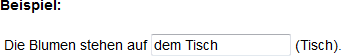
\includegraphics[scale=0.8]{BspLueckentextBlumen}
\caption{Beispiel zum Ausfüllen der Lückentexte}
\label{pic:BspLUE}
\end{figure}

Die Substantive in den relevanten Präpositionalphrasen wurden so gewählt, dass sie im Genitiv keine nennenswerte Schwankung zwischen langer und kurzer Endung (oder gegebenenfalls auch der Nullendung) aufweisen, also nicht zu Zweifeln oder Unsicherheiten führen \citep[zu Zweifelsfällen bei Genitivendungen s. etwa][]{Szczepaniak2014}. Die mögliche Zeichenzahl in den Lücken wurde jeweils so definiert, dass der Eintrag mindestens die Länge der Dativform mit Definitartikel (z.\,B. \object{dem Verkauf}) und maximal die Länge der Genitivform mit Definitartikel und langer Endung (z.\,B. \object{des Verkaufes}) haben kann. 

Als Distraktoren wurden Fremd- und Lehnwörter mit Genusschwankungen gewählt (\object{Annonce, Go-Live, Blog, Laptop, Event}). Diese eigneten sich gut, da die Proband:innen auch in diesen Fällen überlegen müssen, welchen Artikel sie einsetzen. So lenken die Distraktoren die Aufmerksamkeit weg von der Rektion der Präpositionen hin zur Wahl des Genus. Damit liegt aus der Perspektive der Befragten der Fokus auf der Auswahl einer Form des Definitartikels und nicht nur auf Kasusunterschieden. 
\subsection{Assoziationen als Hinweis auf Indexikalitäten} 
\label{sec:Ass}
Die Frage nach möglichen Assoziationen zu den Rektionsvarianten soll zeigen, welche Indexikalitäten den Varianten von den Befragten zugeschrieben werden (zur Indexikalisierung der Varianten s. \autoref{sec:IndexikalitaetRektionskasus}). 
Hier werden den Proband:innen zwei Versionen eines Satzes präsentiert, die sich ausschließlich in der Rektion der enthaltenen Präposition unterscheiden. 
Damit wird ein indirekter Ansatz (\textit{indirect approach}) gewählt, bei dem nicht nach der Einstellung zu einer vordefinierten Kategorie gefragt wird (etwa \object{was denken Sie über den Dativ?}), sondern bei dem mit Stimuli gearbeitet wird~\citep[s.][1251--1252]{Garrett2005}. 

Die Assoziationsabfrage steht bewusst nach dem Produktionsteil, damit die Proband:innen noch nicht für die Kasusvariation sensibilisiert worden sind, wenn sie die Lückentexte ausfüllen.
Mithilfe eines Zufallsgenerators werden die Teilnehmenden bei der Assoziationsabfrage auf vier Gruppen verteilt. 
Jede Gruppe erhält nur ein Satzpaar mit einer der vier Präpositionen. 
So kann die Fragebogenlänge reduziert und dennoch jede der vier Präpositionen abgefragt werden. 
Die Sätze zu den abgefragten Präpositionen sind folgende: 

\ea 
\ea  Ich bin wegen dem Starkregen zu spät gekommen.
\ex  Ich bin wegen des Starkregens zu spät gekommen.
\z 
\ex
\ea Während dem Telefonat mache ich Notizen.
\ex  Während des Telefonats mache ich Notizen.
\z 
\ex
\ea Dank des Brückentags konnte ich ihn besuchen.
\ex Dank dem Brückentag konnte ich ihn besuchen.
\z 
\ex
\ea Sie hat es gegenüber des Lehrers nicht erwähnt.
\ex Sie hat es gegenüber dem Lehrer nicht erwähnt.
\z
\z
Die Befragten werden zunächst gebeten, mögliche Assoziationen zur ersten Variante des präsentierten Satzes zu äußern. Anschließend werden sie nach Assoziationen zur zweiten Satzvariante gefragt. Die Assoziationen können jeweils frei in ein Textfeld eingetragen werden. Die Frage ist offen gehalten (bspw. \glqq welche Assoziationen haben Sie zu Variante~1 (\object{Sie hat es gegenüber des Lehrers nicht erwähnt.})? Bitte notieren Sie, was Ihnen spontan dazu einfällt.\grqq), um keine mögliche Assoziation auszuschließen oder erst hervorzurufen (\autoref{sec:Methodologie}). Die Gestaltung als offene Frage ist hier auch deshalb wichtig, da offene Fragen \glqq den Befragungspersonen die Möglichkeit bieten, so zu sprechen, wie sie es gewohnt sind\grqq{} \citep[s.][739]{PorstSept.1996}. So soll festgestellt werden, ob eine mögliche Indexikalisierung der Varianten Teil des metasprachlichen Wissens der Befragten über die Rektionsvarianten der Präpositionen ist. Ein Nachteil bei offenen Fragen kann sein, dass sie durch eine große Zahl an Antwortkategorien schwer auszuwerten sind, weshalb sie möglichst fokussiert formuliert sein sollten (\citealp[s.][62--63]{Porst2014} sowie \autoref{sec:Methodologie}). Um Nennungen von Assoziationen, die sich nicht auf den Rektionskasus beziehen, möglichst gering zu halten, wurden im Fragebogen deshalb jeweils Satzpaare präsentiert, die sich nur im Kasus der von der Präposition regierten Nominalphrase unterscheiden. 

Schon die Vorgabe einer Anzahl, wie viele freie Nennungen gemacht werden sollen, sehen \citet[216]{Garrett.2004} eher als Nachteil für die Auswertung. 
Tatsächlich kann es interessant sein, sich anzusehen, wie produktiv die Befragten beim Antwortengeben sind~\citep[s.][71]{Adler.2018}. 
Daher wurden den Befragten hier beliebig viele Felder zur Verfügung gestellt. 

Zusätzlich zu den freien Assoziationen wurde abgefragt, inwiefern Proband:innen Personen, die die Variante mit Dativrektion bzw. die Variante mit Genitivrektion äußern, bestimmte Eigenschaften wie z.\,B. \glq gebildet\grq{} zuschreiben. Dies wurde mithilfe semantischer Differenziale (auch \object{Polaritätsprofile} genannt) überprüft (\cites[s.][1255]{Garrett2005}[234]{Atteslander2010}; \autoref{sec:Methodologie}). Bei dieser Methode werden den Befragten mehrere gegensätzliche Eigenschaftspaare präsentiert, die \glqq zu dem Objekt in keinem unmittelbaren sachlichen, jedoch in einem assoziativen Bezug\grqq{} \citep[234]{Atteslander2010} stehen  und die jeweils die Pole einer Skala bilden. In der vorliegenden Untersuchung sollen die Befragten die Rektionsvarianten auf fünfstufigen Skalen zwischen ungebildet~--~gebildet, unsympathisch~--~sympathisch, inkompetent~--~kompetent und unfreundlich~--~freundlich einordnen (s. \autoref{pic:SemDiffSc}). 
Laut \citet[49]{Preston2004} sind sozialer Status und Sympathie die wichtigsten Bewertungsaspekte für sprachliche Varianten (\autoref{sec:Bewertungsgrundlage}), weshalb sie auch hier herangezogen wurden. Die Kombination aus freien Assoziationen und semantischen Differenzialen ermöglicht es, sowohl mögliche unerwartete Antworten zu bekommen als auch die bereits bestehende Hypothese zu überprüfen, dass sich die Varianten in der Bewertung unterscheiden, was sozialen Status und Sympathie angeht.  

\begin{figure}
\centering
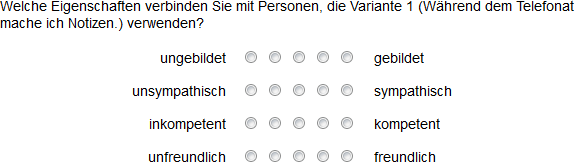
\includegraphics[scale=0.8]{SemDiffSc}
\caption{Semantische Differenziale zu den Rektionsvarianten}
\label{pic:SemDiffSc}
\end{figure}

\subsection{Akzeptabilitätstest} 
\label{sec:Akz}
Der Akzeptabilitätstest besteht aus zwei Teilen, die auf zwei Seiten des Fragebogens aufgeteilt sind. 
Im ersten Teil werden die Proband:innen gebeten, sich eine Situation vorzustellen, die ein formelles Register erfordert: \glqq Stellen Sie sich vor, Sie korrigieren einen förmlichen Brief an ein Amt, den ein guter Freund geschrieben hat. 
Wie würden Sie die sprachliche Form der folgenden Formulierungen bewerten?\grqq{} Im zweiten Teil hingegen erfordert die beschriebene Situation ein eher informelles Register: \glqq Stellen Sie sich vor, Sie unterhalten sich mit einem guten Freund. 
Wie würden Sie die sprachliche Form der folgenden Formulierungen bewerten?\grqq{} 
Wie \citet[182]{Koplenig.2016} zeigen, weisen förmliche Schreiben und Gespräche mit Freunden recht große Unterschiede auf, was die Akzeptabilität von Varianten angeht, die nicht dem geschriebenen Standard zuzuordnen sind. 
Diese Situationen wurden daher gewählt, um die Registrierung der Rektionsvarianten zu überprüfen.

Der Akzeptabilitätstest erfolgt nach der Assoziationsabfrage, damit die Befragten bei der Frage nach möglichen Assoziationen noch nicht von den im Akzeptabilitätstest vorgegebenen Registerunterschieden (formell und informell) beeinflusst werden und ihre Assoziationen möglichst frei äußern können. 

Die Befragten werden für den Akzeptabilitätstest erneut per Zufallsgenerator in vier Gruppen eingeteilt. 
Die Gruppen 1 und 3 bekommen Beispiele mit ursprünglichen Dativpräpositionen, die Gruppen 2 und 4 Beispiele mit ursprünglichen Genitivpräpositionen. 
Die Gruppen 1 und 3 bzw. 2 und 4 unterscheiden sich untereinander darin, welche Präposition in welcher Kondition vorkommt. 
\begin{description}
\item Gruppe 1\\ formeller Teil: \object{gegenüber des Sachbearbeiters}\\ informeller Teil: \object{dank des Urlaubs}
\item Gruppe 2\\ formeller Teil: \object{während dem Vortrag}\\ informeller Teil: \object{wegen dem Urlaub}
\item Gruppe 3\\ formeller Teil: \object{dank des Sachbearbeiters}\\ informeller Teil: \object{gegenüber des Schaffners}
\item Gruppe 4\\ formeller Teil: \object{wegen dem Konto}\\ informeller Teil: \object{während dem Spiel}
\end{description}
Alle Beispiele weisen die jeweils neue, von der ursprünglichen Rektion abweichende Variante auf. 
Es wurde darauf geachtet, dass die Beispiele lexikalisch und semantisch in das jeweilige Setting passen. 
Zusätzlich wurden Distraktoren eingebaut, die sich in den Gruppen nicht unterschieden (z.\,B. \object{Herr Schulzes Geburtstag}). 
In jeder Gruppe wurde außerdem in beiden Konditionen \object{seit} mit Genitivrektion abgefragt:
\begin{description}
\item Alle Gruppen\\ formeller Teil: \object{seit des Sturms}\\ informeller Teil: \object{seit des Festes}
\end{description}
Wie bereits im Produktionsexperiment (\autoref{sec:LU}) dient die Primärpräposition zur Überprüfung der Hypothese, dass auch Primärpräpositionen in bestimmten Kontexten von einigen Sprachbenutzer:innen mit Genitivrektion akzeptiert werden. 
Da davon ausgegangen wurde, dass \object{seit} mit Genitivrektion besonders salient ist, ist dieses Beispiel jeweils das letzte in einem Setting. 

Zu jedem Beispiel werden die Befragten gebeten, zunächst die Korrektheit sowie die Angemessenheit zu bewerten. 
Bei der Korrektheit können sie zwischen \glqq richtig\grqq{} und \glqq falsch\grqq{} entscheiden, bei der Angemessenheit zwischen \glqq in einem förmlichen Brief angemessen\grqq{} und \glqq in einem förmlichen Brief unangemessen\grqq{} bzw. zwischen \glqq in einem Gespräch angemessen\grqq{} und \glqq in einem Gespräch unangemessen\grqq. 
Geben sie an, dass etwas unangemessen ist, so müssen sie in einem Eingabefeld deutlich machen, warum sie es nicht akzeptieren. Auch hierfür wird eine offene Frage verwendet (\glqq was stört Sie?\grqq). 
Des Weiteren wird abgefragt, ob die Proband:innen die im Beispiel präsentierte Form selbst verwenden würden (\glqq würde ich selber schreiben/sagen\grqq) und wie sicher sie sich bei ihrer Antwort sind (\glqq ganz sicher, ziemlich sicher, etwas unsicher, sehr unsicher\grqq). 
Die Frage nach der eigenen Unsicherheit wurde in \citet{Vieregge.2019b} ausgewertet und wird in der vorliegenden Studie nicht weiter berücksichtigt. 

Mit diesem Testdesign können Daten zu mehreren Fragen erhoben werden: Beurteilen die Befragten eine Rektionsvariante generell als korrekt oder empfinden sie sie als Fehler? 
Wie sind die Varianten registriert? 
Wird die Korrektheit einer Variante anders bewertet als ihre Angemessenheit? 
Schreiben die Proband:innen die Verwendung der Varianten lediglich anderen zu oder sehen sie sie auch bei sich selbst? 
Gibt es Unsicherheiten bei der Bewertung der präsentierten Varianten? 
Dass sowohl im Akzeptabilitätstest als auch bei den Assoziationen und im Produktionstest nach konkreten Beispielen der ausgewählten Präpositionen mit Definitartikel und direkt darauf folgendem Substantiv gefragt wird, gewährleistet die Vergleichbarkeit zwischen den drei Fragebogenteilen und damit zwischen Bewertung und Produktion der Varianten. 
Für einen solchen Vergleich ist aufgrund des komplexen Verhältnisses von Einstellungen und Verhalten (\autoref{sec:Spracheinstellungsforschung}) zudem  wesentlich, dass die Erhebung der Einstellung und die Erhebung des Verhaltens (in diesem Fall der Produktion) in folgenden Punkten übereinstimmen \citep[s.][219]{Jonas.2014}: a) Welches Verhalten wird abgefragt (hier: Verwendung des Rektionskasus)? b) Was ist das Objekt des Verhaltens (hier die konkrete Präposition)?, c) In welcher Umgebung wird das Verhalten ausgeführt (hier formelle oder informelle Kondition)? d) In welchem Zeitrahmen wird das Verhalten ausgeführt (im Fragebogen beziehen sich die Fragen immer auf die Gegenwart)?

\subsection{Erhobene Metadaten}
\label{sec:ME}
\largerpage
\begin{sloppypar}
Im letzten Teil des Fragebogens werden personenbezogene Daten erhoben. Dazu gehören zunächst die Muttersprache(n) sowie die Region, in der eine Person größtenteils aufgewachsen ist. 
Nach den Muttersprachen wird mit folgender Formulierung gefragt: \glqq Welche Sprache(n) haben Sie als Muttersprache(n) erlernt (abgeschlossener Spracherwerb vor dem 12. Lebensjahr)?\grqq{} Die Herkunftsregion kann über ein Dropdown-Menü ausgewählt werden. Zur Verfügung stehen folgende Antwortmöglichkeiten: \glqq Norddeutschland (Hamburg, Niedersachsen, Schleswig\hyp Holstein, Bremen)\grqq, \glqq Süddeutschland (Bayern, Baden\hyp Württemberg)\grqq, \glqq Ostdeutschland (Berlin, Brandenburg, Mecklenburg\hyp Vorpommern, Sachsen, Thüringen, Sachsen\hyp Anhalt)\grqq, \glqq Westdeutschland (Nordrhein\hyp Westfalen, Rheinland\hyp Pfalz, Saarland, Hessen)\grqq, \glqq Österreich\grqq, \glqq Schweiz\grqq{} oder \glqq in einem anderen Land\grqq. 
% Änderung Anfang
Die Kategorien Ost und West umfassen damit auch Bundesländer, die ebenso den nördlichen bzw. südlichen Bundesländern hätten zugeordnet werden können (etwa Mecklenburg-Vorpommern oder das Saarland). 
Dies ist der Annahme geschuldet, dass aufgrund der Verbreitung des Fragebogens besonders viele Teilnehmende aus dem Norden (Hamburg, Schleswig-Holstein) und Süden (Bayern und Baden-Württemberg) stammen und die Gruppen bei einer anderen Zuordnung sehr ungleich besetzt wären.
Da ein Vergleich der Gruppen Nord und Süd angestrebt wurde, war zudem vor allem die klare Abgrenzung dieser beiden Regionen wichtig. 
\end{sloppypar}
% Änderung Ende

Ob eine Person einen Dialekt spricht, wird mithilfe einer offenen Frage überprüft: \glqq Wenn Sie in Ihrer Familie, mit Freunden oder in anderen Situationen einen Dialekt sprechen, nennen Sie diesen bitte.\grqq{} %Begründung/Problematisierung\\

Des Weiteren werden Daten zu Bildungsstand und Beruf erbeten. 
Die Befragten können den höchsten von ihnen erzielten Bildungsabschluss über ein Dropdown\hyp Menü auswählen. 
Die Auswahlmöglichkeiten sind hier bewusst zunächst recht ausdifferenziert, sodass die Befragten später zu Gruppen zusammengefasst werden können, ohne dass die genaue Information zur Art ihres Abschlusses verloren geht. 
Bei der Frage nach ihrem Beruf wurden die Befragten gebeten, möglichst genaue Angaben zu machen (\glqq Machen Sie gerne möglichst genaue Angaben, etwa \glq Lehrerin für Mathematik und Chemie\grq{} statt nur \glq Lehrerin\grq [...]\grqq). 
Zusätzlich wurden die Proband:innen gefragt, wie häufig sie im Beruf längere Texte wie z.\,B. Protokolle oder Artikel verfassen oder lesen. 
Hier konnte auf einer fünfstufigen Skala eine Antwortmöglichkeit zwischen \glqq ich verfasse oder lese im Beruf täglich längere Texte\grqq{} und \glqq ich verfasse und lese im Beruf nie längere Texte\grqq{} gewählt werden. 
Diese Daten sind wichtig, um etwa Zusammenhänge zwischen der beruflichen Tätigkeit und der Akzeptabilität oder zwischen dem Bildungsstand und der Produktion zu überprüfen. 

Die im Fragebogen zuletzt abgefragten Metadaten sind das Alter und das Geschlecht. Das Alter lässt sich von den Befragten in ein offenes Feld eintragen, sodass Altersgruppen in einem späteren Schritt gebildet werden können. Bei der Frage nach dem Geschlecht stehen die Antwortmöglichkeiten \glqq weiblich\grqq, \glqq männlich\grqq{} und \glqq anderes\grqq{} zur Auswahl. Abschließend besteht auf der letzten Fragebogenseite die Möglichkeit, Anmerkungen zu machen (\glqq Damit sind wir fast am Ende der Befragung angelangt. Falls Sie noch Anmerkungen zu der Umfrage haben, ist hier Platz dafür.\grqq). 
%Ein Rückschluss darauf, aus welcher Gruppe ein Datensatz stammt, ist über die Variable "{}Referenz"{} möglich. Die den verschiedenen Gruppen zur Verfügung gestellten URLs weisen unterschiedliche Markierungen auf, die als Referenz im Datensatz gespeichert werden. Zum Beispiel Ref=1 für die Fragebögen, die über die in der Facebookgruppe der Studienstiftung des deutschen Volkes geteilte URL aufgerufen wurden. 

\section{Datenerhebung und Aufbereitung der Daten}
\label{sec:DatenerhebungundAufbereitung}
Der Fragebogen war vom 18.01. bis 01.03.2017 online, also insgesamt 42 Tage. Zusätzlich erfolgte eine 25-tägige Nacherhebung vom 25.07. bis 19.08.2017. 

Die erhobenen Daten konnten als csv-Datei vom Server heruntergeladen werden. Im Datensatz wurden zusätzlich zu den Antworten automatisch weitere Variablen gespeichert. Zu nennen sind hier die Fallnummer, Datum und Uhrzeit des Fragebogenaufrufs, die Bearbeitungszeit der einzelnen Seiten, die Bearbeitungszeit des kompletten Fragebogens und der Anteil der fehlenden Antworten. Das Datenset wurde mithilfe von R \citep[][Version 3.6.1]{RCoreTeam2019} und RStudio \citep[][Version 1.2.5033]{RStudio.2019} aufbereitet und ausgewertet.\footnote{Folgende Pakete wurden verwendet: 
reshape \citep[][Version 0.8.8]{Wickham.2018}, 
readr \citep[][Version 1.3.1]{Wickham.2018b},
stringr \citep[][Version 1.4.0]{Wickham.2019}, 
tidyverse \citep[][Version 1.3.0]{Wickham.2019b},
ggbeeswarm \citep[][Version 0.6.0]{Clarke.2017}, 
rockchalk \citep[][Version 1.8.144]{Johnson.2019},
psych \citep[][Version 2.0.7]{Revelle2016},
party \citep[][Version 1.3-4]{Hothorn.2010},
Hmisc \citep[][Version 4.4-0]{Harrell.2020}.} 
Das R-Projekt mit den Skripten findet sich im digitalen Anhang. 
\subsection{Verbreitung des Fragebogens}
\label{sec:VerbreitungFragebogen}
Die Gruppe der deutschsprachigen Internetnutzer ist keinesfalls deckungsgleich mit der Gruppe der Sprecher:innen des Deutschen. \citet{Baur2009} weisen auf mehrere Probleme hin, die sich bei Stichproben in Onlinebefragungen ergeben, von denen hier nur drei genannt werden sollen:
\begin{quote}\textit{Alter: }Je jünger eine Person ist, desto eher hat sie einen Internetanschluss: 2007 nutzten neun von zehn der 14- bis 19-Jährigen das Internet, bei den 60- bis 69-Jährigen war es dagegen nur jeder Dritte und bei den ab 70-Jährigen nur noch jeder Achte.

\textit{Bildung: }2007 nutzten mit 92~Prozent fast alle Schüler das Internet. Bei denjenigen, die ihre Schulzeit beendet haben gilt: Je höher der Bildungsgrad, desto größer die Nutzungswahrscheinlichkeit. So nutzten vier von fünf Personen mit (Fach"~)Hochschulabschluss das Internet, aber nur eine von drei Personen, die die Volkschule besucht, aber keine Lehre gemacht haben.

\textit{Berufsstatus: }Drei Viertel der Berufstätigen, aber nur vier von zehn Nicht-Berufstätigen nutzten 2007 das Internet.~\citep[112--113]{Baur2009}\end{quote}
Onlinebefragungen sind insbesondere jungen Personen mit hohem Bildungsgrad zug{\"a}nglich~\citep[s.][114]{Baur2009}.
Hinzu kommt, \glqq dass {\"A}ltere und gering Gebildete besonders h{\"a}ufig einzelne Fragen nicht beantworten oder die Befragung fr{\"u}hzeitig abbrechen\grqq{}~\citep[123]{Baur2009}.
Um diesen Schwierigkeiten zu begegnen, wurde der Link zum Onlinefragebogen über verschiedene Kanäle verbreitet (s.\,u.). So sollten Personen unterschiedlicher sozialer Gruppen erreicht werden. Eine sukzessive Verbreitung sollte außerdem sicherstellen, dass eventuelle Fehler korrigiert werden können, bevor der Fragebogen allen Proband:innen zugänglich ist. Es waren jedoch keine weiteren Korrekturen nötig.

Folgender Einladungstext wurde zusammen mit der URL zum Fragebogen verschickt: 
\begin{quote}
\textbf{Befragung zum Umgang mit Sprache}\\
Im Rahmen meiner Doktorarbeit an der Universität Hamburg führe ich eine wissenschaftliche Studie dazu durch, wie Menschen über die deutsche Sprache denken und wie sie mit sprachlichen Fragen umgehen.\\
Sie sind herzlich eingeladen, an der Online-Befragung zu diesem Thema teilzunehmen: \url{https://www.soscisurvey.de/Umgang\_mit\_Sprache/} \\
Für die Studie spielt es keine Rolle, wie oft und wie gerne Sie über Sprache nachdenken. Wichtig ist nur, dass Deutsch Ihre Muttersprache ist. \\
Vielen Dank für Ihre Teilnahme!
\end{quote}
Diese Teilnahmeeinladung wurde über folgende Kanäle verbreitet: über die Facebookgruppe der Studienstiftung des Deutschen Volkes, über die Facebookgruppe der Promovierenden der Geisteswissenschaften der Universität Hamburg, über die Couchsurfing-Facebookgruppe Hamburg, als Kommentar zu einem Beitrag des Facebookauftritts der Bundesregierung zum Tag der Muttersprache, über das schwarze Brett auf der internen Homepage einer Hamburger Kantorei, über das Forum Stipnetz (Stipendiatennetzwerk), über Weiterleitungen von Kolleg:innen und Freund:innen z.\,B. an Mitarbeiter:innen eines biologischen Instituts in Norddeutschland, Pfleger:innen eines Altersheims in Würzburg, Psychologiestudierende in Würzburg und einen Chor in Nürnberg. 

Da sich unter den Befragten der ersten Erhebungsphase ein sehr geringer Anteil an Befragten über 65 Jahre und an Befragten ohne Hochschulabschluss befand, wurde der Fragebogen im Zuge einer Nacherhebung über die E\hyp Mailverteiler einer Ornithologengruppe und einer Hamburger Seniorenkantorei sowie über Weiterleitungen an Kontakte in einem Tischtennisverein und bei einer Feuerwehr verbreitet.\footnote{Ich danke allen Kolleg:innen, Freund:innen und Verwandten, die mir bei der Verbreitung des Fragebogens geholfen haben.}

\subsection{Ausgeschlossene Fälle}
\label{sec:Ausschluss}
Berücksichtigt wurden nur die Antworten der Befragten, die den gesamten Fragebogen bis zur letzten Seite ausgefüllt haben. 
Außerdem wurden acht Teilnehmer:innen ausgeschlossen, die Deutsch nicht als Muttersprache angegeben hatten.
Ebenfalls ausgeschlossen wurden drei Teilnehmer:innen aus Österreich und zwei Teilnehmer:innen mit einer anderen Herkunft.\footnote{Da sich die Sprachsituation in Österreich und in anderen Ländern von der in Deutschland unterscheidet, konnten diese Befragten nicht ohne Weiteres in die Auswertung integriert werden. Aufgrund der geringen Anzahl Befragter aus anderen Ländern als Deutschland war jedoch auch kein systematischer Vergleich möglich.} 

Personen, die einen Fragebogen nicht sorgfältig und ernsthaft ausgefüllt haben, und deren Antworten daher bei der Auswertung nicht berücksichtigt werden sollten, können relativ zuverlässig im Nachhinein identifiziert werden: Das zuverlässigste Maß scheint hier die zum Ausfüllen benötigte Zeit zu sein \citep[s.][]{Leiner.2019}. \citet{Leiner.2019} schlägt als Maß den Relative Speed Index (RSI) vor: 
\begin{quote} For each page, the sample's median page completion time is divided by the individual completion time, resulting in a speed factor. A factor of 2 means that the respondent has completed a page twice as fast as the typical respondent.~\citep[236]{Leiner.2019} 
\end{quote}
SoSci-Survey berechnet den RSI für jeden ausgefüllten Fragebogen automatisch und speichert ihn im Datensatz ab. In der vorliegenden Studie wurden die neun Fälle mit einem RSI von über 2 überprüft. Da es jedoch bei keinem dieser Fälle Hinweise darauf gab, dass der Fragebogen nicht sorgfältig ausgefüllt wurde, wurden sie nicht aussortiert. Alle Befragten mit RSI-Werten über 2 hatten auch offene Fragen beantwortet und teilweise sogar recht viele Nennungen eingetragen, sodass davon ausgegangen werden kann, dass es sich schlicht um besonders schnelle Proband:innen handelt. 
\section[Qualitative Inhaltsanalyse der freien Angaben]{Qualitative Inhaltsanalyse der freien Angaben: Kategorisierung und Kodierung}
\label{sec:Kategorisierung}
Die Assoziationen mit den Rektionsvarianten und die Begründung, warum eine Variante im Akzeptabilitätstest als unangemessen eingestuft wurde, konnten im Fragebogen frei in Textfelder eingetragen werden. Die Auswertung dieser Antworten erfolgte nach dem Verfahren der qualitativen Inhaltsanalyse. 
Nach \citet[][]{Schreier.2014} wird darunter
\begin{quote}
ein Verfahren zur Beschreibung ausgewählter Textbedeutungen verstanden. Diese Beschreibung erfolgt, indem relevante Bedeutungen als Kategorien eines inhaltsanalytischen Kategoriensystems expliziert und anschließend Textstellen den Kategorien dieses Kategoriensystems zugeordnet werden. \citep[5]{Schreier.2014}
\end{quote} 
Die qualitative Inhaltsanalyse erfolgt im Wesentlichen in folgenden Schritten: Auf Grundlage von Forschungsfragen und Hypothesen werden Daten erhoben. Anschließend werden Kodierungseinheiten festgelegt, ein Kategoriensystem entwickelt und Regeln zur Kodierung aufgestellt \citep[s.][49]{Kuckartz.2014}. Es gibt unterschiedliche Auffassungen dazu, wie bei der Kategorienbildung vorgegangen werden sollte bzw. was diese ausmacht.
\citet[2]{Schreier.2014} fasst zusammen, dass diese sich darin unterscheiden, ob sie ein theoriegeleitetes (deduktives), am Material orientiertes (induktives) oder ein gemischt deduktives und induktives Vorgehen vorschlagen. 
In der vorliegenden Studie wird ein eher induktiver Ansatz verfolgt. 

Im Anschluss an die Kategorienbildung erfolgen mehrere Kodierungsdurchgänge. 
Unter Kodierung wird \glqq die Zuordnung von Kategorien zu relevanten Textpassagen bzw. die Klassifikation von Textmerkmalen verstanden\grqq{} \citep[56]{Kuckartz2010}. 
Für die Überprüfung der Qualität des Kategoriensystems eignet sich die Berechnung der Intra- und Intercoderreliabilität \citep[s.][49--50]{Kuckartz.2014}. Schließlich kann das Material anhand der Kodierungen ausgewertet werden \citep[s.][78]{Kuckartz.2014}. 
%\subsection{Kategorisierung und Kodierung der Zweifelsfälle und der Lösungsstrategien}
%\label{sec:KategorisierungZF}
%Im Falle der Zweifelsfälle erfolgte die Kategorienbildung deduktiv auf Grundlage der Zweifelsfälleeinteilung von \citet{Klein2003} (s.~\autoref{cha:Zweifelsfaelle}) gebildet. Die genannten Zweifelsfälle wurden in Microsoft Excel in folgende Kategorien sortiert: phonologisch, morphologisch, morphosyntaktisch, pragmatisch, unklar und Kommentar. Es handelt sich damit um inhaltliche Kategorien nach \citet[Melanie fragen, ob die Abbildung von ihr ist]{Kuckartz2012}. Die Nennungen der persönlichen Zweifelsfälle der Befragten wurden von zwei Hilfskräften annotiert. Die Annotationsrichtlinien finden sich im Anhang. Ein erster Annotationsdurchgang ergab eine Übereinstimmung der Kategorien von ??. Nach diesem ersten Durchgang wurden die Annotationsrichtlinien noch einmal verfeinert. \\ 
\subsection{Kategorisierung und Kodierung der Assoziationen}
\label{sec:KategorisierungAss}
Die Kodierung der Assoziationen erfolgte in \citet{MAXQDA.19892018}. Hierfür wurden aus den Daten acht Tabellendokumente erstellt und in \citeauthor{MAXQDA.19892018} importiert: 
für jede Präposition je ein Dokument mit den Assoziationen zur Dativvariante und eines mit den Assoziationen zur Genitivvariante. 
Neben den Assoziationen sind in den Tabellen Angaben zu Beruf, Alter und Gender der Befragten enthalten. 
Den Dokumenten wurden die Variablen \glqq Rektionskasus im Beispiel\grqq, \glqq ursprünglicher Kasus\grqq, \glqq Präposition\grqq{} und \glqq Beispielsatz im Fragebogen\grqq{} zugewiesen. 
\autoref{table:DokumenteAss} bietet eine Übersicht über die in \citeauthor{MAXQDA.19892018} importierten Dokumente. 
Das \citeauthor{MAXQDA.19892018}-Projekt mit den kategorisierten Assoziationen findet sich im digitalen Anhang. 
\largerpage[-1]

\begin{longtable}{ll}
\caption{Dokumente mit Assoziationsantworten in \citeauthor{MAXQDA.19892018} und deren Eigenschaften}\label{table:DokumenteAss}\\
\lsptoprule\endfirsthead
\midrule\endhead
\multicolumn{2}{l}{Assoziationen zu  \object{wegen} + Dativ}\\
 & Rektionskasus im Beispiel: Dativ\\
 & ursprünglicher Kasus: Genitiv  \\                               
 & Präposition: \object{wegen}   \\                                       
 & Beispielsatz: \object{Ich bin wegen dem Starkregen zu spät gekommen.}\\
\addlinespace
\multicolumn{2}{l}{Assoziationen zu  \object{wegen} + Genitiv} \\
 & {Rektionskasus im Beispiel: Genitiv}                            \\
 & {ursprünglicher Kasus: Genitiv}                                 \\ 
 & {Präposition: \object{wegen}}                                            \\ 
 & {Beispielsatz: \object{Ich bin wegen des Starkregens zu spät gekommen.}} \\
\tablevspace
\multicolumn{2}{l}{Assoziationen zu \object{während} + Dativ} \\    
& {Rektionskasus im Beispiel: Dativ}                              \\
& {ursprünglicher Kasus: Genitiv}                                 \\ 
& {Präposition: \object{während}}                                          \\ 
& {Beispielsatz: \object{Während dem Telefonat mache ich Notizen.}}        \\
\tablevspace
\multicolumn{2}{l}{Assoziationen zu \object{während} + Genitiv} \\ 
& {Rektionskasus im Beispiel: Genitiv}                            \\
& {ursprünglicher Kasus: Genitiv}                                 \\ 
& {Präposition: \object{während}}                                          \\ 
& {Beispielsatz: \object{Während des Telefonats mache ich Notizen.}}      \\
\tablevspace
\multicolumn{2}{l}{Assoziationen zu \object{dank} + Genitiv}  \\   
& {Rektionskasus im Beispiel: Genitiv}                            \\
& {ursprünglicher Kasus: Dativ}                                   \\ 
& {Präposition: \object{dank}}                                             \\ 
& {Beispielsatz: \object{Dank des Brückentags konnte ich ihn besuchen.}}   \\
\addlinespace
\multicolumn{2}{l}{Assoziationen zu \object{dank} + Dativ}  \\     
& {Rektionskasus im Beispiel: Dativ}                              \\
& {ursprünglicher Kasus: Dativ}                                   \\ 
& {Präposition: \object{dank}}                                             \\ 
& {Beispielsatz: \object{Dank dem Brückentag konnte ich ihn besuchen.}}    \\
\tablevspace
\multicolumn{2}{l}{Assoziationen zu \object{gegenüber} + Genitiv} \\
& {Rektionskasus im Beispiel: Genitiv}                            \\
& {ursprünglicher Kasus: Dativ}                                   \\ 
& {Präposition: \object{gegenüber}}                                        \\ 
& {Beispielsatz: \object{Sie hat es gegenüber des Lehrers nicht erwähnt.}} \\
\tablevspace
\multicolumn{2}{l}{Assoziationen zu \object{gegenüber} + Dativ} \\ 
& {Rektionskasus im Beispiel: Dativ}                              \\
& {ursprünglicher Kasus: Dativ}                                   \\ 
& {Präposition: \object{gegenüber}}                                        \\ 
& {Beispielsatz: \object{Sie hat es gegenüber dem Lehrer nicht erwähnt.}}  \\ 
\lspbottomrule
\end{longtable}

Folgende Schritte wurden bei der Kategorisierung und Kodierung der Assoziationen vorgenommen: 
\begin{enumerate}
\sloppy
\item Erster Kodierungsdurchgang in \citeauthor{MAXQDA.19892018} an einem repräsentativen Sample  (jeder Kasus bei jeder Präposition, unterschiedliche Altersgruppen) und dabei Erstellung des Kategoriensets
\item Erstellung eines Handbuchs
\item Kompletter Kodierungsdurchgang in \citeauthor{MAXQDA.19892018} 
\item Zweiter kompletter Kodierungsdurchgang und Berechnung der Intracoderreliabilität
\item Ein Viertel der Assoziationen zusätzlich von zwei Hilfskräften kodiert (wieder repräsentatives Sample), Berechnung der Intercoderreliabilität
\item Bei Nichtübereinstimmung: Einfache Fälle werden entschieden, alle anderen werden im Team besprochen. 
\end{enumerate}
Zunächst wurde induktiv ein Kategoriensystem entwickelt. 
Hierfür wurde ein Sample von 80 Antworten aus den Daten ausgewählt, das Antworten zu jeder der vier abgefragten Präpositionen und jeweils beiden Rektionsvarianten enthielt (als eine Antwort zählt dabei jeweils der gesamte Eintrag, den eine befragte Person gemacht hat). 
Zusätzlich wurde darauf geachtet, dass im Sample Antworten von Befragten verschiedener Alters- und Bildungsgruppen enthalten sind. 
Im Zuge der Kategorienbildung wurden den Antworten zunächst Kategorien eines relativ niedrigen {Abstraktions\-niveaus} zugeordnet, wie etwa \glqq hohe Bildung\grqq{} im Falle von Aussagen, die eine gebildete Person mit einer Variante assoziieren. 
Diese Kategorien wurden anschließend zu Oberkategorien zusammengefasst, die die Kategorien der niedrigeren Abstraktionsniveaus inhaltlich bündeln. 
Im Anschluss an die Entwicklung des Kategoriensystems wurde ein Handbuch erstellt, das zu allen Kategorien und Unterkategorien eine kurze Erläuterung und Beispiele enthält. 
Das Handbuch findet sich im digitalen Anhang. 
Mithilfe des Handbuchs erfolgte ein erster kompletter Kodierungsdurchgang, im Zuge dessen das Kategoriensystem und das Handbuch noch einmal verfeinert und an einigen Stellen erweitert wurden. 
Das so entstandene endgültige Kategoriensystem umfasst 16 Oberkategorien mit bis zu drei Ebenen von Unterkategorien (insgesamt 72 Kategorien). 
Die inhaltlich bündelnden Oberkategorien sind folgende: 
%\newpage 
\begin{multicols}{2}
\begin{enumerate}
\item Person
\item Formalität
\item Medium 
\item Varietät 
\item Ästhetik
\item Korrektheit 
\item Gleichgültigkeit 
\item eigener Sprachgebrauch
\item Zweifel
\item Sprachwandel 
\item Stellung 
\item Bedeutung und Verständlichkeit 
\item Herleitung 
\item nicht relevant 
\item keine Assoziation
\item nicht entscheidbar 
\end{enumerate}
\end{multicols}

\noindent Auf die genaue Zusammensetzung der Ober- und Unterkategorien wird im Zuge der Ergebnisdarstellung in \autoref{sec:ErgAss} näher eingegangen. 
Zusätzlich wurden die in die Dokumente übernommenen Metadaten Alter und Gender kodiert, sodass in \citeauthor{MAXQDA.19892018} auf die Altersguppe bzw. das Geschlecht der Befragten zugegriffen werden kann. 

Als Kodierungseinheiten dient jeweils die gesamte Antwort einer Person zu einer Variante,  bspw. \object{Schreiben, formell, Abstand, Fremder}. 
Einer Kodierungseinheit können mehrere Kategorien und Unterkategorien zugeordnet sein, im Falle des angeführten Beispiels  etwa \glqq Medium > schriftlich\grqq, \glqq Formalität > formell\grqq{} und \glqq Person > Vertrautheit > Fremdheit/Distanz\grqq.
Wichtig ist außerdem, dass die zu kodierenden Antworten immer nur der untersten Kategorienebene zugeordnet wurden. 
Damit wurde sichergestellt, dass jede Kodierungsentscheidung so differenziert wie möglich erfolgte.
Bspw. war es auf diese Weise nicht möglich, eine Antwort lediglich der Oberkategorie \glqq Person\grqq{} zuzuordnen, ohne zu spezifizieren, auf welche Eigenschaft eines Personentypus Bezug genommen wird. 
Die Oberkategorien enthalten aber jeweils alle Kodierungen der darunterliegenden Kategorien, sodass später schnell ersichtlich ist, wie viele Assoziationen bspw. insgesamt in den Bereich Personentypus fallen.

%\autoref{table:KategorienAss} bietet einen Überblick über das Kategoriensystem. 
%%\begin{landscape}
%%\begin{longtable}{llll}
%%\caption{Kategoriensystem für die Kategorisierung der Assoziationen}\\
%%\label{table:KategorienAss}
%%\textbf{Oberkategorie}                                                    & \textbf{Unterkategorien 1}                                                          & \textbf{Unterkategorien 2}         &
%%\textbf{Unterkategorien 3}                                     \\
%%\endfirsthead
%%\caption{Kategoriensystem für die Kategorisierung der Assoziationen, Fortsetzung}\\
%%\textbf{Oberkategorie}                                                    & \textbf{Unterkategorien 1}                                                          & \textbf{Unterkategorien 2}         &
%%\textbf{Unterkategorien 3}                                     \\                                             \\
%%\endhead
%%\midrule
%%\endfoot
%%\endlastfoot
%%\hline
%%Person                                                                    &                                   &                                        &                                 \\
%                                                                          & %Vertrautheit                      &                                        &                                 \\
%                                                                          &                                   %& Vertrautheit/Nähe                      &                                 \\
%                                                                          &                                   %& Fremdheit/Distanz                      &                                 \\
%                                                                          & %Charakter                         &                                        &                                 \\
%                                                                          &                                   %& präzise/professionell/vertrauenswürdig &                                 \\
%                                                                          &                                   %& vornehm/altmodisch                     &                                 \\
%                                                                          &                                   %& sympathisch/mir ähnlich                &                                 \\
%                                                                          &                                   %& besserwisserisch                       &                                 \\
%                                                                          &                                   %& unfreundlich                           &                                 \\
%                                                                          &                                   %& streng/seriös                          &                                 \\
%                                                                          &                                   %& locker/unprätentiös                    &                                 \\
%                                                                          &                                   %& abgehoben/arrogant                     &                                 \\
%                                                                          &                                   %& pedantisch/verkrampft                  &                                 \\
%                                                                          &                                   %& nachlässig/schlampig                   &                                 \\
%                                                                          & %bestimmte Gruppe                  &                                        &                                 \\
%                                                                          &                                   %& geringes Prestige                      &                                 \\
%                                                                          &                                   %&                                        & Arbeiter:innen                   \\
%                                                                          &                                   %&                                        & Unterschicht                    \\
%                                                                          &                                   %&                                        & Technische Berufe               \\
%                                                                          &                                   %& hohes Prestige                         &                                 \\
%                                                                          &                                   %&                                        & Akademiker:innen/\\ Gymnasiast:innen\end{tabular} \\
%                                                                          &                                   %&                                        & Beruflich Erfolgreiche          \\
%                                                                          &                                   %&                                        & Bourgeoisie                     \\
%                                                                          &                                   %& Ältere Leute                           &                                 \\
%                                                                          &                                   %& Kinder                                 &                                 \\
%                                                                          &                                   %& Junge Leute                            &                                 \\
%                                                                          & %Bildung                           &                                        &                                 \\
%                                                                          &                                   %& niedrige Bildung                       &                                 \\
%                                                                          &                                   %& hohe Bildung                           &                                 \\
%                                                                          & %Sprachkompetenz                   &                                        &                                 \\
%                                                                          &                                   %& hohe Sprachkompetenz                   &                                 \\
%                                                                          &                                   %& mangelnde Sprachkompetenz              &                                 \\
%                                                                          \hline
%%eigener Sprachgebrauch                                                    &                                   &                                        &                                 \\
%                                                                          & %entspricht eigenem Gebrauch nicht &                                        &                                 \\
%                                                                          & %entspricht eigenem Gebrauch       &                                        &                                 \\
%                                                                          
%                                                                         \hline
%%Zweifel                                                                   &                                   &                                        &                                 \\
%%\hline
%%Register                                                                  &                                   &                                        &                                 \\
%                                                                          & %informell                         &                                        &                                 \\
%                                                                          & %formell                           &                                        &                                 \\
%                                                                          \hline
%%Medium                                                                    &                                   &                                        &                                 \\
%                                                                          & %schriftlich                       &                                        &                                 \\
%                                                                          & mündlich                          &                                        &                                 \\
%                                                                          \hline
%Varietät                                                                  &                                   &                                        &                                 \\
%                                                                          & Standard                          &                                        &                                 \\
%                                                                          & Regionalsprache/Dialekt           &                                        &                                 \\
%                                                                          & umgangs-/alltagssprachlich        &                                        &                                 \\
%                                                                          \hline
%Korrektheit                                                               &                                   &                                        &                                 \\
%                                                                          & falsch                            &                                        &                                 \\
%                                                                          & richtig                           &                                        &                                 \\
%                                                                          \hline
%Gleichgültigkeit                                                          &                                   &                                        &                                 \\
%\hline
%Stellung                                                                  &                                   &                                        &                                 \\
%\hline
%Ästhetik                                                                  &                                   &                                        &                                 \\
%                                                                          & simpel                            &                                        &                                 \\
%                                                                          & auffällig/ungewohnt               &                                        &                                 \\
%                                                                          & unauffällig/normal                &                                        &                                 \\
%                                                                          & nicht ästhetisch                  &                                        &                                 \\
%                                                                          &                                   & schlecht/unschön                       &                                 \\
%                                                                          &                                   & umständlich                            &                                 \\
%                                                                          &                                   & gestelzt/abgehoben/überkorrekt         &                                 \\
%                                                                          &                                   & plump/schlampig                        &                                 \\
%                                                                          & ästhetisch                        &                                        &                                 \\
%                                                                          &                                   & elegant/gehoben                        &                                 \\
%                                                                          &                                   & gut/schön                              &                                 \\
%                                                                          \hline
%Sprachwandel                                                              &                                   &                                        &                                 \\
%                                                                          & natürlicher Wandel                &                                        &                                 \\
%                                                                          & Sprachverfall                     &                                        &                                 \\
%                                                                          \hline
%Bedeutung und \\ Verständlichkeit\end{tabular} &                                   &                                        &                                 \\
%\hline
%Herleitung                                                                &                                   &                                        &                                 \\
%\hline
%nicht relevant                                                            &                                   &                                        &                                 \\
%\hline
%keine Assoziation                                                         &                                   &                                        &                                 \\
%\hline
%nicht entscheidbar                                                        &                                   &                                        &                                
%\end{longtable}
%\end{landscape}
Nach einem zeitlichen Abstand von sechs Wochen erfolgte ein zweiter Kodierungsdurchlauf am kompletten Datensatz. 
Zusätzlich wurde das repräsentative Sample, an dem der erste Durchlauf vorgenommen wurde, von zwei Hilfskräften kodiert. 
Nur ein solches mehrstufiges Kodierungsverfahren kann die Verlässlichkeit der Kodierung sichern. 
Wie verlässlich die Kodierung ist, lässt sich daran ablesen, wie hoch die Übereinstimmung der Kodierungsdurchläufe ist \citep[s.][557]{Artstein.2008}. 
Dafür wird zum einen die Intracoderreliabilität berechnet, also die Übereinstimmung des ersten mit dem zweiten eigenen Durchlauf, zum anderen die Intercoderreliabilität, also die Übereinstimmung der verschiedenen Kodiererinnen untereinander. 
Intra- und Intercoderreliabilität werden hier mit dem Maß Cohen's $\kappa$ angegeben (\citealp[s.][]{Cohen.1960}; für eine Diskussion verschiedener Übereinstimmungsmaße s. \citealp{Artstein.2008}).
Dabei handelt es sich um einen zufallskorrigierten Koeffizienten, d.\,h., die Übereinstimmung der vergebenen Kategorien wird mit dem Anteil der möglicherweise zufälligen Übereinstimmung verrechnet. 
\citet{Doring2016} setzen folgende Grenzwerte für Cohen's $\kappa$ an: \begin{quote} Werte über 0,75 gelten nach konventionellen Standards als sehr gut, Werte zwischen 0,60 und 0,75 werden als gut eingestuft und Werte zwischen 0,40 und 0,60 als mittelmäßige bzw. gerade noch ausreichende Messgenauigkeit eingeordnet. \citep[346]{Doring2016} \end{quote}
Cohen's $\kappa$ lässt sich in \citeauthor{MAXQDA.19892018} berechnen. 
Die Intracoderreliabilität für die Kodierung der Assoziationen beträgt $\kappa=0{,}88$.
Die Intercoderreliabilität zwischen dem eigenen zweiten Durchgang und den Kodierungen der Hilfskräfte beträgt $\kappa=0{,}75$.
Die Übereinstimmung unter den vier Kodierungsdurchläufen der drei Kodiererinnen ist also insgesamt gut bis sehr gut und die Verlässlichkeit der Kodierung somit sehr hoch. 
\subsection{Kategorisierung und Kodierung der Begründungen für die Unangemessenheit einer Variante}
\label{sec:KategorisierungAkz}
Im Akzeptabilitätstest wurden die Befragten gebeten, eine Begründung anzugeben, falls sie eine der präsentierten Varianten als unangemessen eingestuft hatten (\autoref{sec:Akz}). 
Diese Begründung konnten sie frei in ein Textfeld eintragen. 
Wie die freien Assoziationen wurden auch die freien Antworten aus dem Akzeptabilitätstest inhaltsanalytisch kategorisiert. 
Das dafür verwendete Kategorienset orientiert sich an dem bereits für die Assoziationen verwendeten.
Dies hat den Vorteil, dass die Antworten dadurch vergleichbar gemacht werden und sich bei der Auswertung gut Bezüge zwischen den freien Assoziationen und den Begründungen für die Bewertung als unangemessen herstellen lassen. 
Das Kategorienset wurde allerdings an einigen Stellen an die geänderten Anforderungen angepasst, die sich daraus ergaben, dass im Akzeptabilitätstest explizit nach dem für die Ablehnung ausschlaggebenden Aspekt gefragt wird (\glqq was stört Sie?\grqq). 
Die 16 Oberkategorien (\autoref{sec:KategorisierungAss}) blieben dabei weitestgehend erhalten. 
Sie wurden allerdings um die Kategorie \glqq nur Vorschlag oder Benennung\grqq{} ergänzt. 
Diese zusätzliche Kategorie war wichtig, da sich die Auswertung auf Begründungen für die Einstufung als unangemessen konzentriert und Antworten ohne begründendes Element daher von solchen abgegrenzt werden mussten, die eine Begründung erkennen lassen. 
Als weitere Kategorie für die Begründungen kam das \glqq Sprachgefühl\grqq{} hinzu. 

Das Vorgehen bei der Kodierung der freien Antworten aus dem Akzeptabilitätstest war das gleiche wie bei der Kodierung der Assoziationen. 
An einem repräsentativen Sample wurde zunächst die Eignung des aus der Assoziationskodierung bestehenden Kategoriensets überprüft. 
Bei diesem ersten Durchgang wurden die eben erwähnten Anpassungen vorgenommen. 
Anschließend wurde ein Handbuch für die Kodierung erstellt, welches sich im digitalen Anhang befindet. 
Danach erfolgte die Kodierung des kompletten Datensatzes in \citeauthor{MAXQDA.19892018} sowie die Kodierung eines Viertels der Antworten durch zwei Hilfskräfte. 
Die Intracoderreliabilität für die Begründungen der Einstufung als unangemessen im Akzaptabilitätstest beträgt $\kappa=0{,}82$ und zeigt damit eine sehr gute Übereinstimmung \citep[s.][346]{Doring2016}. 
Die Intercoderreliabilität liegt mit $\kappa=0{,}61$ im Bereich guter Übereinstimmung. 
Das \citeauthor{MAXQDA.19892018}-Projekt mit den kategorisierten Begründungen aus dem Akzeptabilitätstest befindet sich im digitalen Anhang. 

\chapter[Auswertung der Onlinebefragung zur Kasusrektion]{Auswertung der Onlinebefragung zur Kasusrektion von \object{wegen}, \object{während}, \object{dank}, \object{gegenüber} und \object{seit}}
\label{cha:Ergebnisse}
Im folgenden Kapitel werden die Ergebnisse aus der Onlinebefragung zum Zusammenhang zwischen Metapragmatik und Sprachgebrauch der Rektionskasus von \wegen, \waehrend, \dank{} und \gegenueber{} sowie der Primärpräposition \object{seit} präsentiert. 
Die Analyse richtet sich dabei nicht nach der Reihenfolge der Erhebung der Daten im Fragebogen, sondern leitet sich aus dem Forschungsinteresse ab und ermöglicht eine schrittweise Datenanalyse:
Einleitend wird ein Überblick über die Zusammensetzung der Gruppe der Befragten gegeben (\autoref{sec:Befragte}).
Dabei werden auch die allgemeinen Ansichten über Sprache thematisiert, die die Befragten im Fragebogen äußern. 
\autoref{sec:ErgAss} widmet sich den freien Assoziationen, die Befragte mit den Rektionsvarianten haben, sowie den semantischen Differenzialen. 
Vor dem Hintergrund der Ergebnisse der Assoziationsstudie werden anschließend die Angaben im Akzeptabilitätstest (\autoref{sec:ErgAkz}) sowie die Kasuswahl im Produktionsexperiment (\autoref{sec:ErgProduktion}) ausgewertet und interpretiert. % Änderung Anfang
Sowohl für die Akzeptabilität als auch für die Produktion wird mithilfe statistischer Modelle (\textit{random forests}) die Relevanz der unterschiedlichen Einflussfaktoren überprüft.%Änderung Ende
%Schließlich wirft \autoref{sec:ErgPositionierung} einen Blick darauf, wie sich einzelne ausgewählte Befragte im Verlauf des Fragebogens zu den Rektionsvarianten positionieren. 
\section{Zusammensetzung der Befragtengruppe}
\label{sec:Befragte}
An der Befragung nahmen 397 Personen teil, die angaben, deutsche MuttersprachlerInnen zu sein und in Deutschland zu leben. 
Im Folgenden wird vorgestellt, wie sich die Gruppe bezüglich soziodemografischer Merkmale sowie hinsichtlich der Angaben zu Sprachbewusstheit, Sprachsicherheit und Variationstoleranz zusammensetzt. 
Dabei geht es zunächst um Alter und Gender der Befragten (\autoref{sec:AlterundGender}), dann um ihre regionale Herkunft und die Dialektkompetenz (\autoref{sec:HerkunftundDialekt}), ihren Bildungsstand (\autoref{sec:Bildung}) und anschließend darum, wie häufig Befragte in ihrem Beruf mit längeren Texten zu tun haben (\autoref{sec:Beruf}). 
\autoref{sec:Sprachbewusstheit} bis \autoref{sec:Variationstoleranz} thematisieren die Angaben der Befragten auf den Likertskalen zu Sprachbewusstheit, Sprachsicherheit und Variationstoleranz.  
\subsection{Alter und Gender der Befragten}
\label{sec:AlterundGender}
234 Befragte gaben an, weiblichen Geschlechts zu sein, 155 gaben an, männlichen Geschlechts zu sein und eine Person gab an, ein anderes Geschlecht zu haben (s. \autoref{table:GenderAnh} im Anhang). 
Sieben Personen machten keine Angabe zu ihrem Geschlecht. 
Der Anteil weiblicher Befragter überwiegt demnach mit 59~\%. 39~\% der Befragten sind männlich. 

Die Befragten sind zwischen 18 und 85 Jahre alt. 
Das Durchschnittsalter liegt bei 37, die Standardabweichung bei 16,2. 
Für die Auswertung werden folgende vier Altersgruppen zusammengefasst: 18--25, 26--35, 36--60 und 61--85 (s. \autoref{table:AltersgruppenAnh} im Anhang).
Der Anteil junger TeilnehmerInnen überwiegt: Über 60~\% der Befragten sind unter 36 Jahre alt.
Aus diesem Grund wurden bei den ersten beiden Altersguppen kleinere Spannen angelegt als bei den beiden letzteren. 
Insgesamt gehören 104 Befragte (ca. 26~\%) der jüngsten Altersgruppe an und 144 (ca. 36~\%) der Gruppe der 26- bis 35-Jährigen.
Nur etwas über 30~\% der Befragten sind 36 Jahre oder älter:
82 Personen (ca. 21~\%) sind 36 bis 60 Jahre alt und 47 Befragte (knapp 12~\%) finden sich in der Gruppe der über 60-Jährigen. 
Ungefähr 5~\% der BefragungsteilnehmerInnen machen keine Altersangabe.

\autoref{pic:AlterundGender} zeigt, wie sich Gender und Alter zueinander verhalten. 
In allen Altersgruppen überwiegt der Anteil weiblicher Befragter, in der Gruppe der 18- bis 25-Jährigen sind prozentual jedoch besonders viele weibliche Befragte vertreten. 
Hier ist das Verhältnis von weiblichen zu männlichen Befragten 68 zu 30~\%. 

\begin{figure}
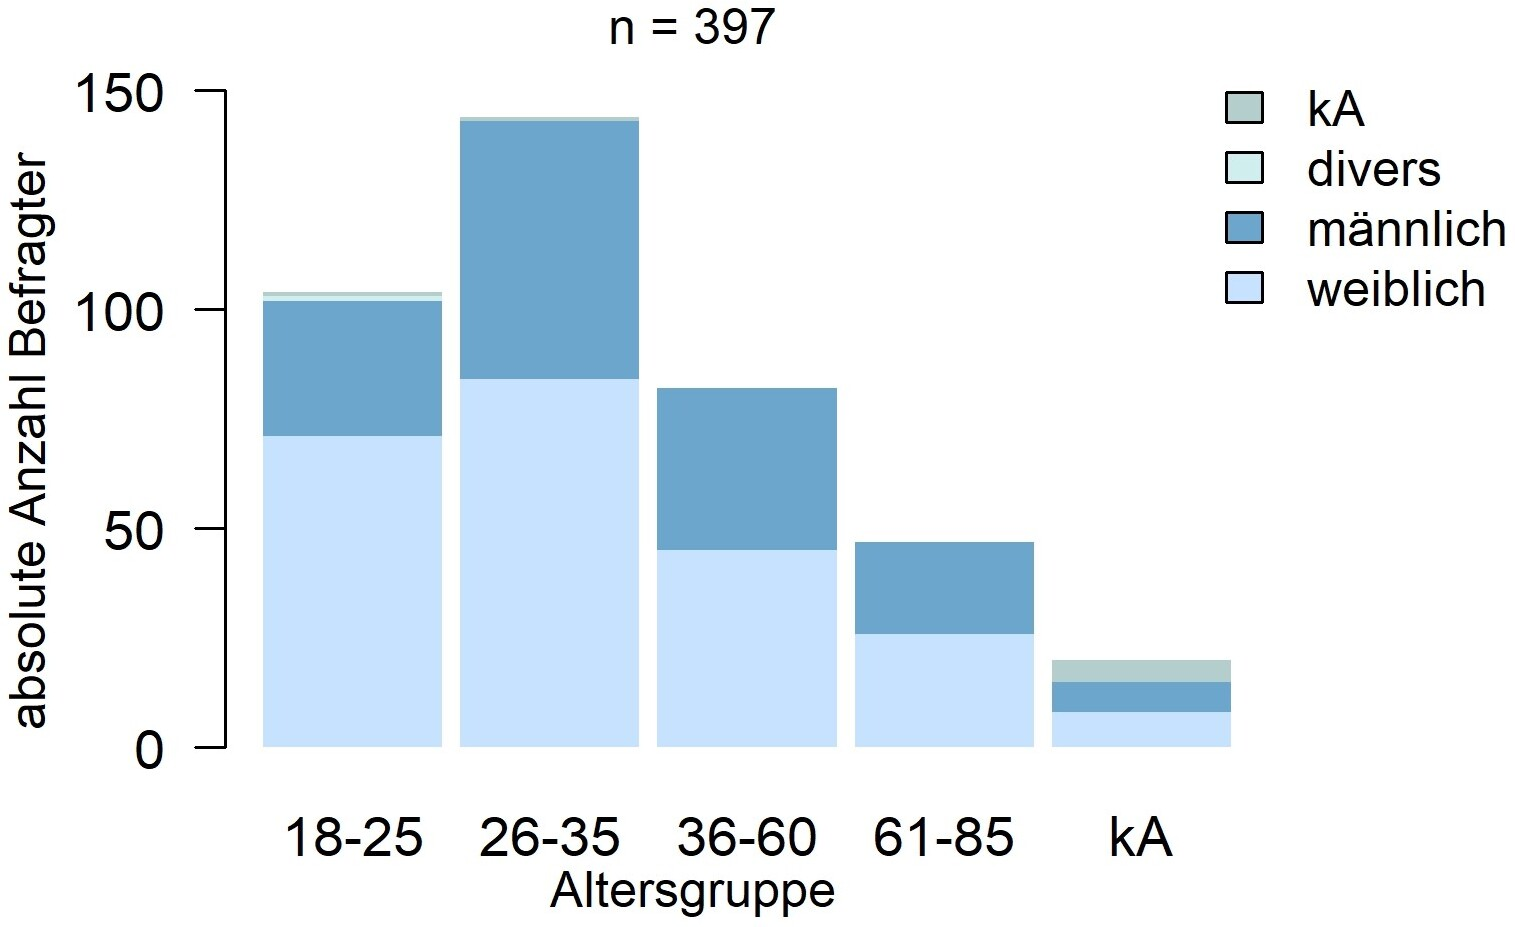
\includegraphics[width=\textwidth]{AlterundGender.jpg}
\caption{Genderzusammensetzung der Altersgruppen}
\label{pic:AlterundGender}
\end{figure}
%\begin{table}
%\centering
%\begin{tabular}{lrrrrrrrrr}
%\textbf{}             & \multicolumn{2}{l}{weiblich} & \multicolumn{2}{l}{männlich} & \multicolumn{2}{l}{divers} & \multicolumn{2}{l}{kA} & \multicolumn{1}{l}{gesamt} \\ \hline
%\textbf{18-25 Jahre}  & 71         & (68 \%)         & 31         & (30 \%)         & 1         & (1 \%)         & 1            & (1 \%)            & 104                        \\ \hline
%\textbf{26-35 Jahre}  & 84         & (58 \%)         & 59         & (41 \%)         & 0         & (0 \%)         & 1            & (1 \%)            & 144                        \\ \hline
%\textbf{36-60 Jahre}  & 45         & (55 \%)         & 37         & (45 \%)         & 0         & (0 \%)         & 0            & (0 \%)            & 82                         \\ \hline
%\textbf{61-85 Jahre}  & 26         & (55 \%)         & 21         & (45 \%)         & 0         & (0 \%)         & 0            & (0 \%)            & 47                         \\ \hline
%\textbf{kA} & 8          & (40 \%)         & 7          & (35 \%)         & 0         & (0 \%)         & 5            & (25 \%)           & 20                         \\ \hline
%\end{tabular}
%\caption{Genderzusammensetzung der Altersgruppen}
%\label{table:AlterundGender}
%\end{table}

\subsection{Regionale Herkunft und Dialektkompetenz der Befragten}
\label{sec:HerkunftundDialekt}
Die Befragten sind regional über ganz Deutschland verteilt, wenn auch ungleichmäßig (für die genauen Zahlen s. \autoref{table:HerkunftAnh} im Anhang): 
Ca. 43~\% der Befragten kommen aus norddeutschen Bundesländern, zu denen Schleswig-Holstein, Niedersachsen, Bremen und Hamburg gerechnet werden. 
% Änderung Anfang
Jeweils ca. ein Viertel der TeilnehmerInnen stammt aus südlichen (Bayern und Baden-Württemberg) oder westlichen bzw. südwestlichen (Nordrhein-Westfalen, Hessen, Rheinland-Pfalz und Saarland) Bundesländern und nur 6,5~\% kommen aus einem östlichen oder nordöstlichen Bundesland (Brandenburg, Mecklenburg-Vorpommern, Sachsen, Thüringen, Sachsen-Anhalt, Berlin).\footnote{Diese Einteilung wurde so vorgenommen, da das Ungleichgewicht zwischen den Befragtengruppen Nord oder Süd und den Gruppen Ost bzw. West bspw. bei Zuordnung von Mecklenburg-Vorpommern zu Norddeutschland vermutlich noch stärker gewesen wäre.
Ein zweiter Grund war die Vergleichbarkeit zwischen der Befragtengruppe aus dem Norden und derjenigen aus dem Süden (s. \autoref{sec:ErgAkzNachRegion} und \autoref{sec:ErgProdNachHerkunft}, vgl. auch \autoref{sec:ME}).}
% Änderung Ende

Betrachtet man die regionale Herkunft nach dem Alter der Befragten, fällt auf, dass die Verteilung nicht in allen Altersgruppen gleich ist (s. \autoref{pic:AlterundHerkunft}). 
In der Gruppe der über 60-Jährigen stammen mit 79~\% deutlich mehr Personen aus norddeutschen Bundesländern als in den anderen Altersgruppen. 
Unter den 18- bis 25-Jährigen ist dagegen der Anteil der Befragten aus Süddeutschland erhöht. 
Andersherum heißt dies auch, dass unter den norddeutschen Befragten besonders viele ältere Personen sind, während sich unter den süddeutschen Befragten besonders viele jüngere Personen finden. 
Dies lässt sich dadurch erklären, dass die Nacherhebung, bei der gezielt ältere Personen gewonnen werden sollten, insbesondere über den Mailverteiler eines norddeutschen Seniorenchors erfolgte (\autoref{sec:VerbreitungFragebogen}). 
Das Ungleichgewicht muss bei späteren Vergleichen nach Alter oder Herkunft der Befragten berücksichtigt werden. 
\begin{figure}
\centering
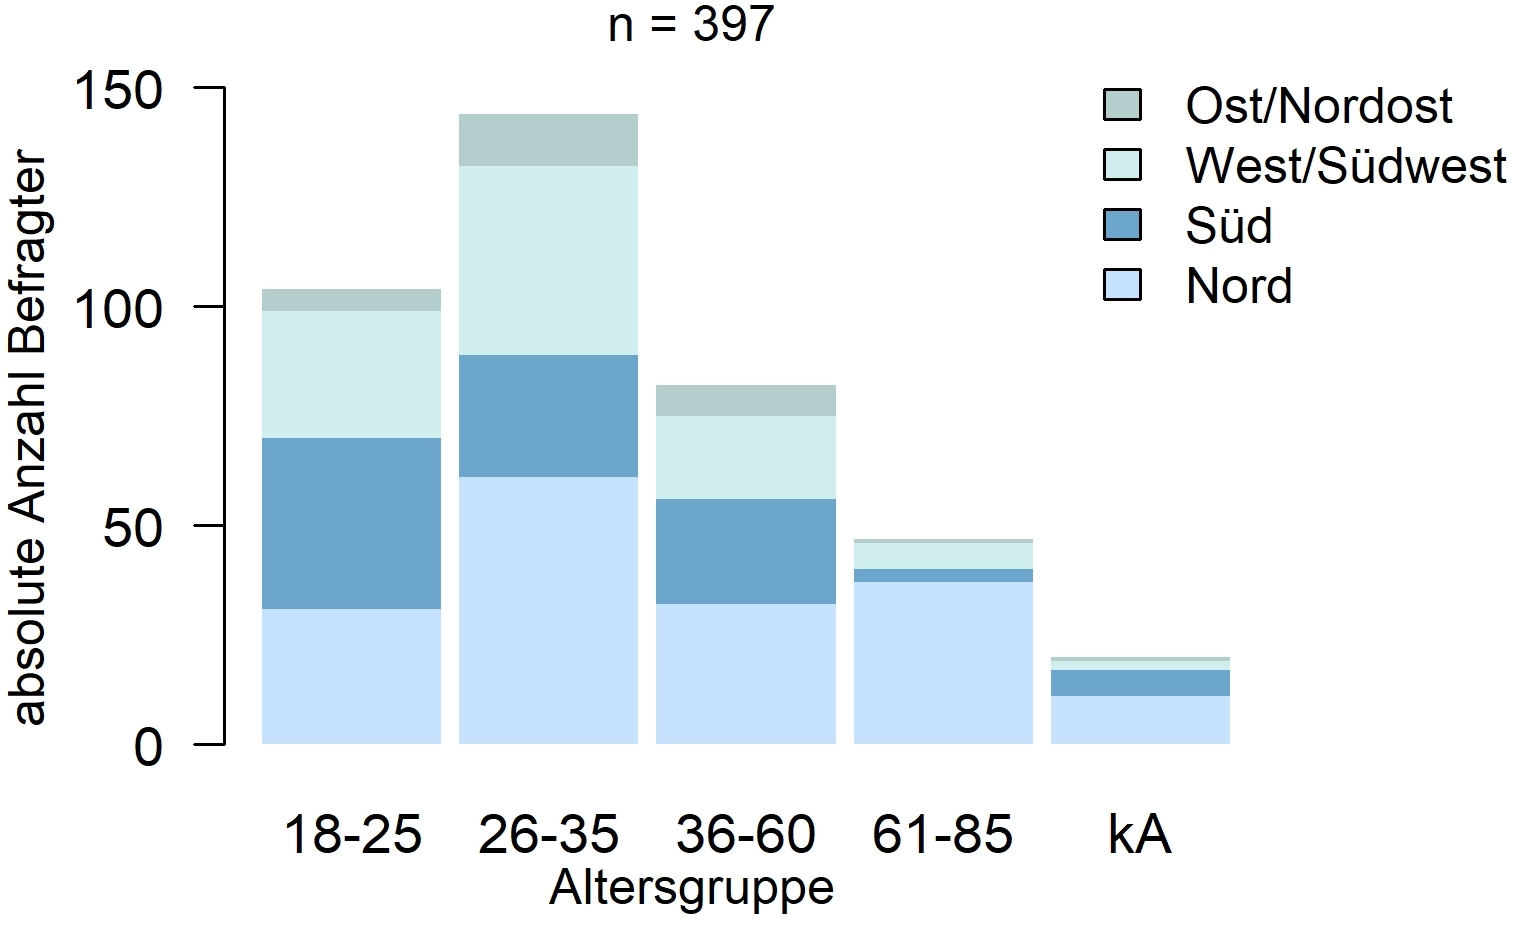
\includegraphics[width=\textwidth]{AlterundHerkunft.jpg}
\caption{Regionale Herkunft in den einzelnen Altersgruppen}
\label{pic:AlterundHerkunft}
\end{figure}
%\begin{table}
%\centering
%\begin{tabular}{lrrrrrrrrr}
%\textbf{}             & \multicolumn{2}{l}{Nord} & \multicolumn{2}{l}{Süd} & \multicolumn{2}{l}{Ost} & \multicolumn{2}{l}{West} & gesamt \\ \hline
%\textbf{18-25 Jahre}  & 31       & (30 \%)       & 39       & (38 \%)      & 5        & (5 \%)       & 29       & (28 \%)       & 104    \\ \hline
%\textbf{26-35 Jahre}  & 61       & (42 \%)       & 28       & (19 \%)      & 12       & (8 \%)       & 43       & (30 \%)       & 144    \\ \hline
%\textbf{36-60 Jahre}  & 32       & (39 \%)       & 24       & (29 \%)      & 7        & (9 \%)       & 19       & (23 \%)       & 82     \\ \hline
%\textbf{61-85 Jahre}  & 37       & (79 \%)       & 3        & (6 \%)       & 1        & (2 \%)       & 6        & (13 \%)       & 47     \\ \hline
%\textbf{keine Angabe} & 11       & (55 \%)       & 6        & (30 \%)      & 1        & (5 \%)       & 2        & (10 \%)       & 20     \\ \hline
%\end{tabular}
%\caption{Regionale Herkunft in den einzelnen Altersgruppen}
%\label{table:AlterundHerkunft}
%\end{table}

In einer offenen Frage wurde nach der Dialektkompetenz der TeilnehmerInnen gefragt. 
Von allen Befragten geben 160 (40~\%) an, dass sie in ihrer Familie, mit Freunden oder in anderen Situationen einen Dialekt sprechen. 
Da eine freie Angabe des Dialekts möglich war, fallen die Antworten sehr unterschiedlich aus: 
Genannt werden teils spezifische Dialekte wie Moselfränkisch, teils Regionalsprachen wie Norddeutsch.  
Einige Antworten enthalten außerdem Angaben zur Intensität des Dialekts (\object{leichtes Fränkisch}) sowie zur Häufigkeit der Nutzung (\object{selten Kölsch}). 
Da diese sehr heterogenen Selbstauskünfte kaum quantitativ interpretierbar sind, werden sie im Folgenden nicht für die Auswertung herangezogen.

Der Anteil der Befragten, die einen Dialekt angeben, ist je nach regionaler Herkunft unterschiedlich hoch. 
Besonders hoch ist der Anteil an DialektsprecherInnen unter Befragten aus Süd- oder Ostdeutschland: 
75~\% der Befragten aus süddeutschen Bundesländern und ungefähr 54~\% der Befragten aus ostdeutschen Bundesländern geben an, einen Dialekt zu sprechen. 
Von den TeilnehmerInnen aus westdeutschen Bundesländern tut dies dagegen nur ein Drittel.
Im Norden ist der Anteil der DialektsprecherInnen mit ca. 22~\% am geringsten. 
\subsection{Bildungsstand der Befragten}
\label{sec:Bildung}
Die Angaben zum höchsten Bildungsabschluss zeigen, dass 66~\% der Befragten einen Hochschulabschluss haben (mindestens Bachelor). 7~\% aller Befragten sind sogar promoviert oder habilitiert (s. \autoref{table:BildungsstandAnh} im Anhang). 
Ca. 32~\% haben keinen Hochschulabschluss. 
Fünf Personen geben einen anderen Abschluss an, z.\,B. Zweites Staatsexamen. 
Für die spätere Untersuchung von Unterschieden in Akzeptabilität und Kasuswahl bei Befragten verschiedener Bildungsstände werden die Befragten auf zwei Bildungsgruppen aufgeteilt: 
Befragte mit Hochschulabschluss (insgesamt 267) und Befragte ohne Hochschulabschluss (insgesamt 130). 
Auch die fünf Befragten, die einen anderen Abschluss angaben, konnten jeweils einer dieser beiden Gruppen zugeordnet werden.\footnote{Vier Befragte, die als Abschluss ein Staatsexamen oder ein Diplom angegeben hatten, wurden der Gruppe mit Hochschulabschluss zugeordnet; eine Person, die den Abschluss Industriemeister angegeben hatte, wurde der Gruppe ohne Hochschulabschluss zugeordnet.}

In \autoref{pic:BildungNachAlter} ist dargestellt, wie sich die Altersgruppen bezüglich der Bildungsstände zusammensetzen.
\begin{figure}
\centering
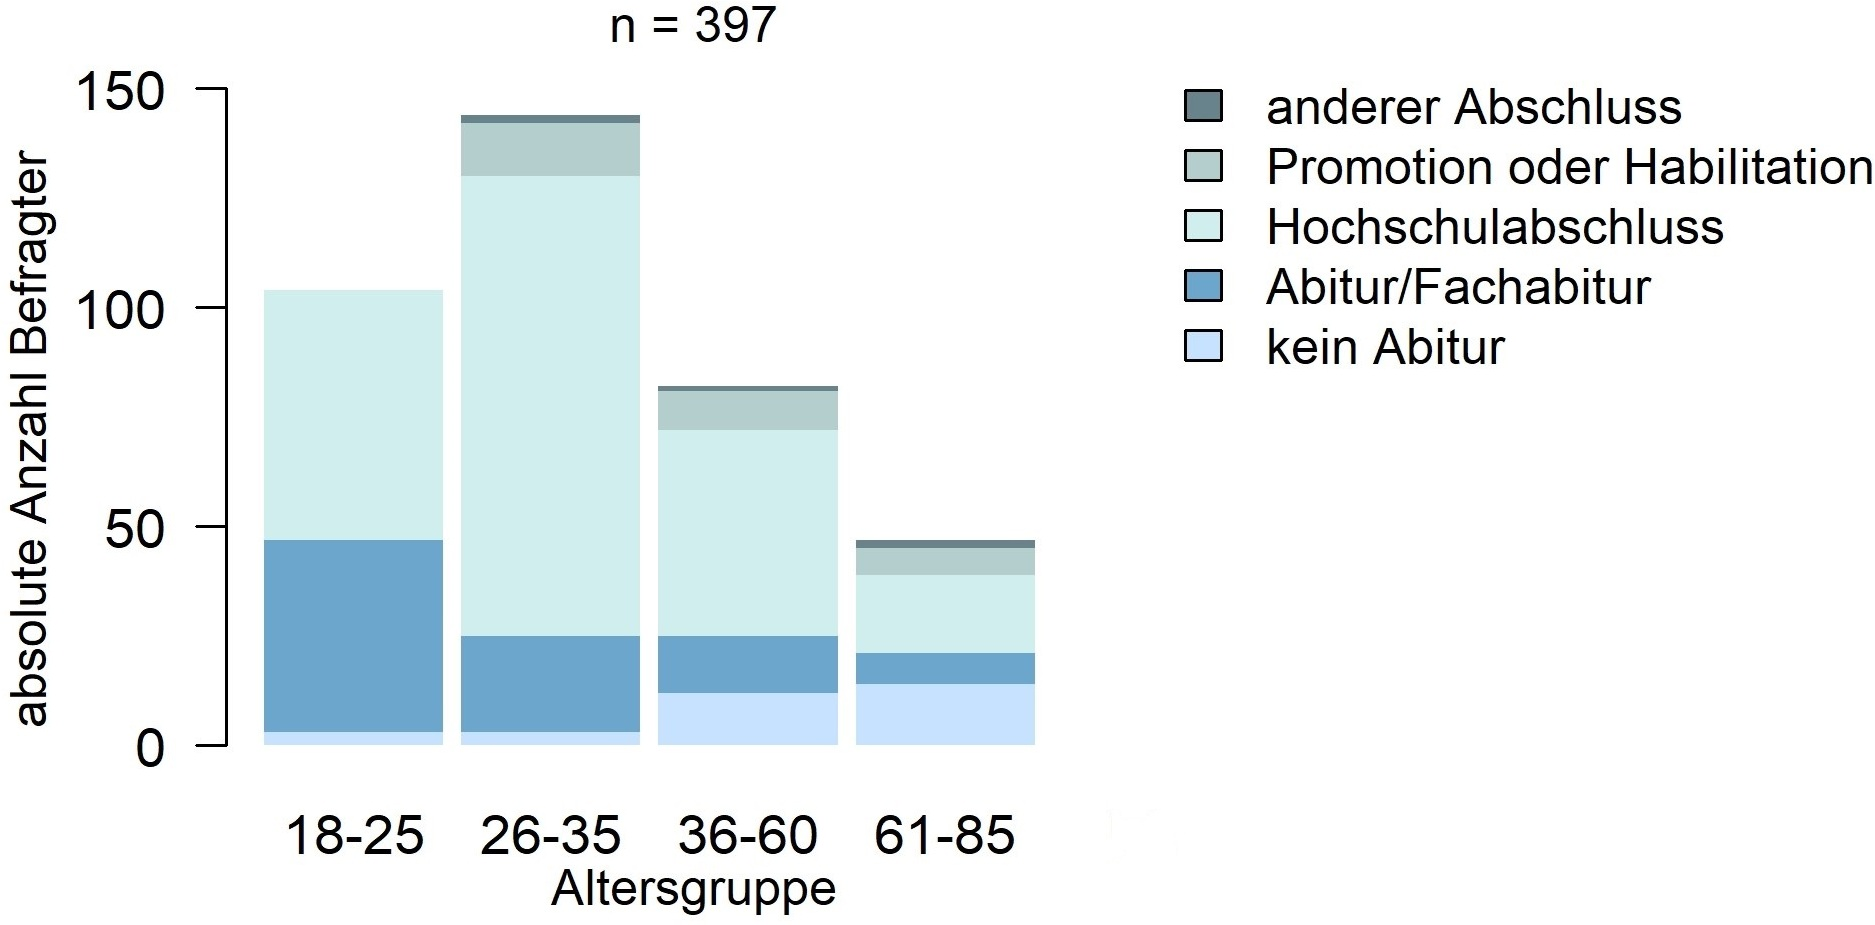
\includegraphics[width=\textwidth]{BildungNachAlter.jpg}
\caption{Bildungsstand der Befragten nach ihrer Altersgruppe}
\label{pic:BildungNachAlter}
\end{figure}
 
Die Aufschlüsselung nach Altersgruppen macht deutlich, dass sich Personen ohne Abitur vor allem unter den Befragten über 35 finden. 
Hier haben insgesamt 20~\% kein Abitur, während es bei den unter 36-Jährigen lediglich 2,4~\% sind. 
Schaut man sich nur die über 60-Jährigen Befragten an, zeigt sich, dass hier sogar beinahe 30~\% angeben, kein Abitur zu haben. 
Der Anteil Befragter ohne Hochschulabschluss ist in beiden Altersgruppen zwar dennoch etwa gleich, jedoch liegt dies zum Teil daran, dass die jüngeren Befragten ihr Studium zum Zeitpunkt der Befragung noch nicht abgeschlossen haben.
Das Ungleichgewicht in der Verteilung der Bildungsabschlüsse muss bei der späteren Analyse von Zusammenhängen zwischen der Bewertung und Verwendung der Rektionskasus mit Alter oder Bildung bedacht werden. 

% s. Alter und Bildung.R
Vergleicht man die regionale Herkunft von Befragten mit Hochschulabschluss und Befragten ohne Hochschulabschluss, fallen keine nennenswerten Unterschiede in der Verteilung auf (s. \autoref{table:AnhHerkunftundHSA} im Anhang). 
\subsection{Textaffinität der Berufe der Befragten}
\label{sec:Beruf}
Um eine Auskunft darüber zu erhalten, wie intensiv die Befragten in ihrem jeweiligen Beruf mit Sprache zu tun haben, wurde danach gefragt, wie häufig sie im Beruf längere Texte verfassen oder lesen (\glqq wie häufig verfassen oder lesen Sie in Ihrem Beruf längere Texte wie zum Beispiel Protokolle oder Artikel?\grqq). 
\autoref{pic:SchreibenLesen} zeigt die Verteilung der Antworten. 
\begin{figure}
\centering
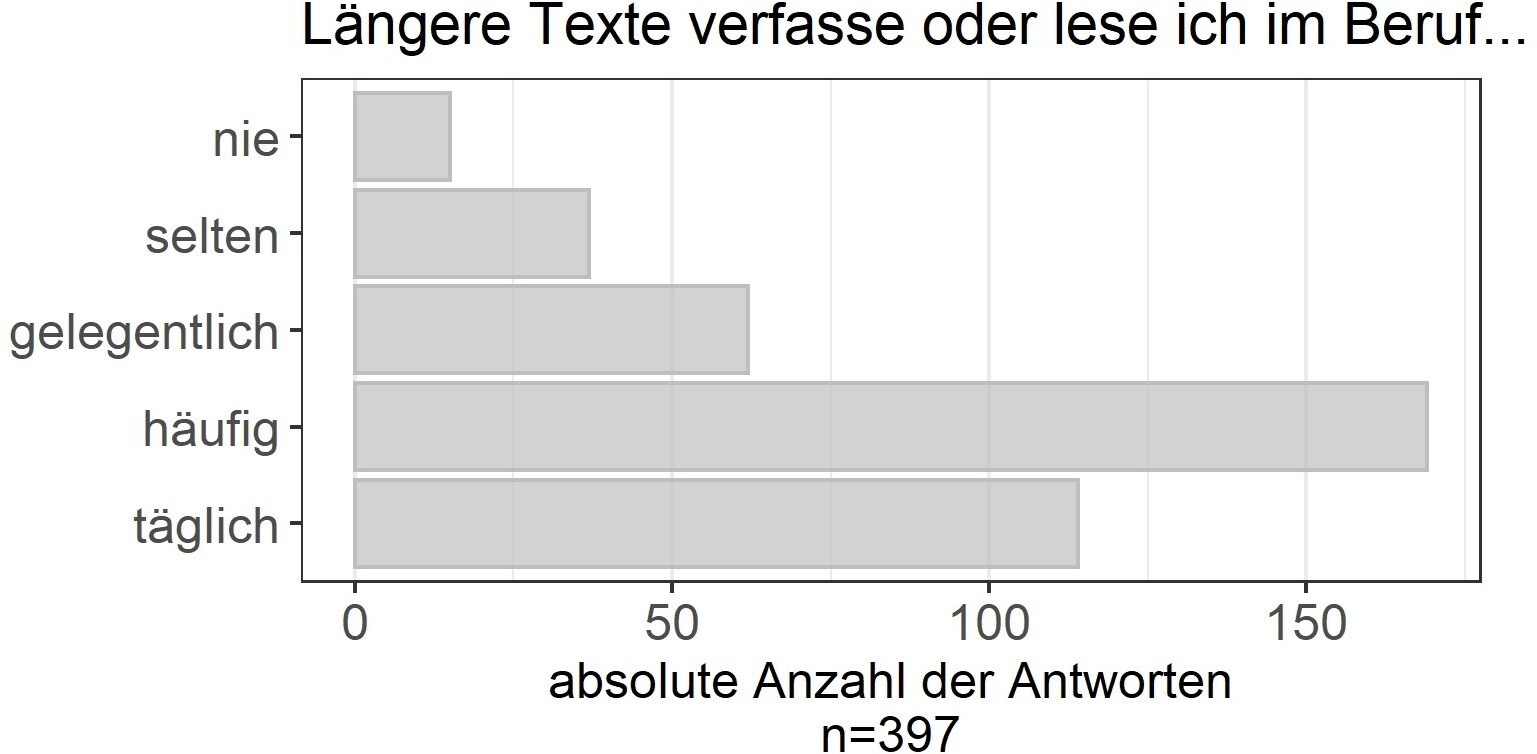
\includegraphics[width=\textwidth]{TextaffinitaetBeruf.jpg}
\caption{Umgang mit längeren Texten im Beruf}
\label{pic:SchreibenLesen}
\end{figure}

Die meisten Befragten geben an, dass sie beruflich häufig oder sogar täglich mit längeren Texten zu tun haben.
Bei 71~\% der Befragten handelt es sich also um beruflich geübte SchreiberInnen und LeserInnen.\footnote{Einzelne TeilnehmerInnen wiesen im Kommentar am Ende des Fragebogens darauf hin, dass die Texte, mit denen sie zu tun haben, größtenteils nicht deutsch sind, sondern bspw. englisch.}
Hierzu zählen etwa LehrerInnen, Studierende und wissenschaftliche MitarbeiterInnen. 
Tatsächlich ist die Gruppe der im Schreiben und Lesen geübten Befragten eventuell sogar noch etwas größer, da Befragte möglicherweise auch außerhalb ihres Berufs mit längeren Texten zu tun haben, etwa wenn sie viele Romane lesen oder einen Vereinsnewsletter betreuen. 
Für die Befragung ist jedoch insbesondere die berufliche Beschäftigung mit längeren Texten relevant, da davon ausgegangen werden kann, dass diese erstens mit einer recht großen Sorgfalt und zweitens mit einer recht hohen Kompetenz in Fragen sprachlicher Normen einhergeht. 

16~\% der Befragten geben an, beruflich gelegentlich mit längeren Texten zu tun zu haben. 
Auch in dieser Gruppe finden sich relativ viele Studierende (14 von 62 Personen) sowie einige Personen, die in den Bereichen Pädagogik/Erziehung arbeiten, und bspw. kaufmännische Berufe.
Nur 52 Befragte (13~\%) geben an, dass sie im Beruf selten oder nie längere Texte verfassen oder lesen. 
Darunter finden sich ebenfalls Studierende, aber auch bspw. Angestellte aus den Bereichen Hotel/Gastronomie und Pflege/Medizin, GrafikerInnen sowie Hausfrauen. 

Für die spätere Untersuchung von Zusammenhängen zwischen Akzeptabilität und Kasuswahl mit der Textaffinität des Berufs lassen sich die Befragten aufteilen in die Gruppe derer, die im Beruf häufig oder sogar täglich mit längeren Texten zu tun haben (Beruf textaffin) und die Gruppe derer, die im Beruf nie bis gelegentlich mit längeren Texten zu tun haben (Beruf nicht textaffin): 
Insgesamt 283 Befragte haben einen textaffinen Beruf, 114 haben einen Beruf, der nicht textaffin ist. 
\subsection{Sprachbewusstheit der Befragten}
\label{sec:Sprachbewusstheit}
Bereits die Angaben zum Umgang mit längeren Texten im Beruf deuten auf eine recht große Sprachaffinität der TeilnehmerInnen hin. 
Um darüber hinaus zu überprüfen, inwiefern sich die Befragten selbst als sprachbewusst, sprachlich sicher und variationstolerant einschätzen, wurde mit drei Likertskalen gearbeitet:
Einer zur Sprachbewusstheit, einer zur Sprachsicherheit sowie einer zur sprachlichen Variation. 
Jede der drei Likertskalen besteht aus mehereren Aussagen (Items), zu denen die Befragten ihre Zustimmung bzw. Ablehnung signalisieren sollen (\autoref{sec:RE}). 
Die Skala zur Sprachbewusstheit enthält folgende drei Aussagen: 
\begin{enumerate}
\item Ich denke häufig über die deutsche Sprache nach.
\item Mit dem Thema Sprache beschäftige ich mich nur sehr selten.
\item Ich interessiere mich für die deutsche Sprache. 
\end{enumerate}

\noindent Die Auswertung der Likertskala zur Sprachbewusstheit zeigt, dass die Befragten überwiegend recht interessiert an Sprache sind. 
\autoref{pic:SB} gibt einen Überblick über die Beantwortung der einzelnen Items der Skala. 
Die genauen Zahlen sind außerdem in \autoref{table:LikertZsfsgAnh} im Anhang zusammengefasst. 
\begin{figure}
\centering
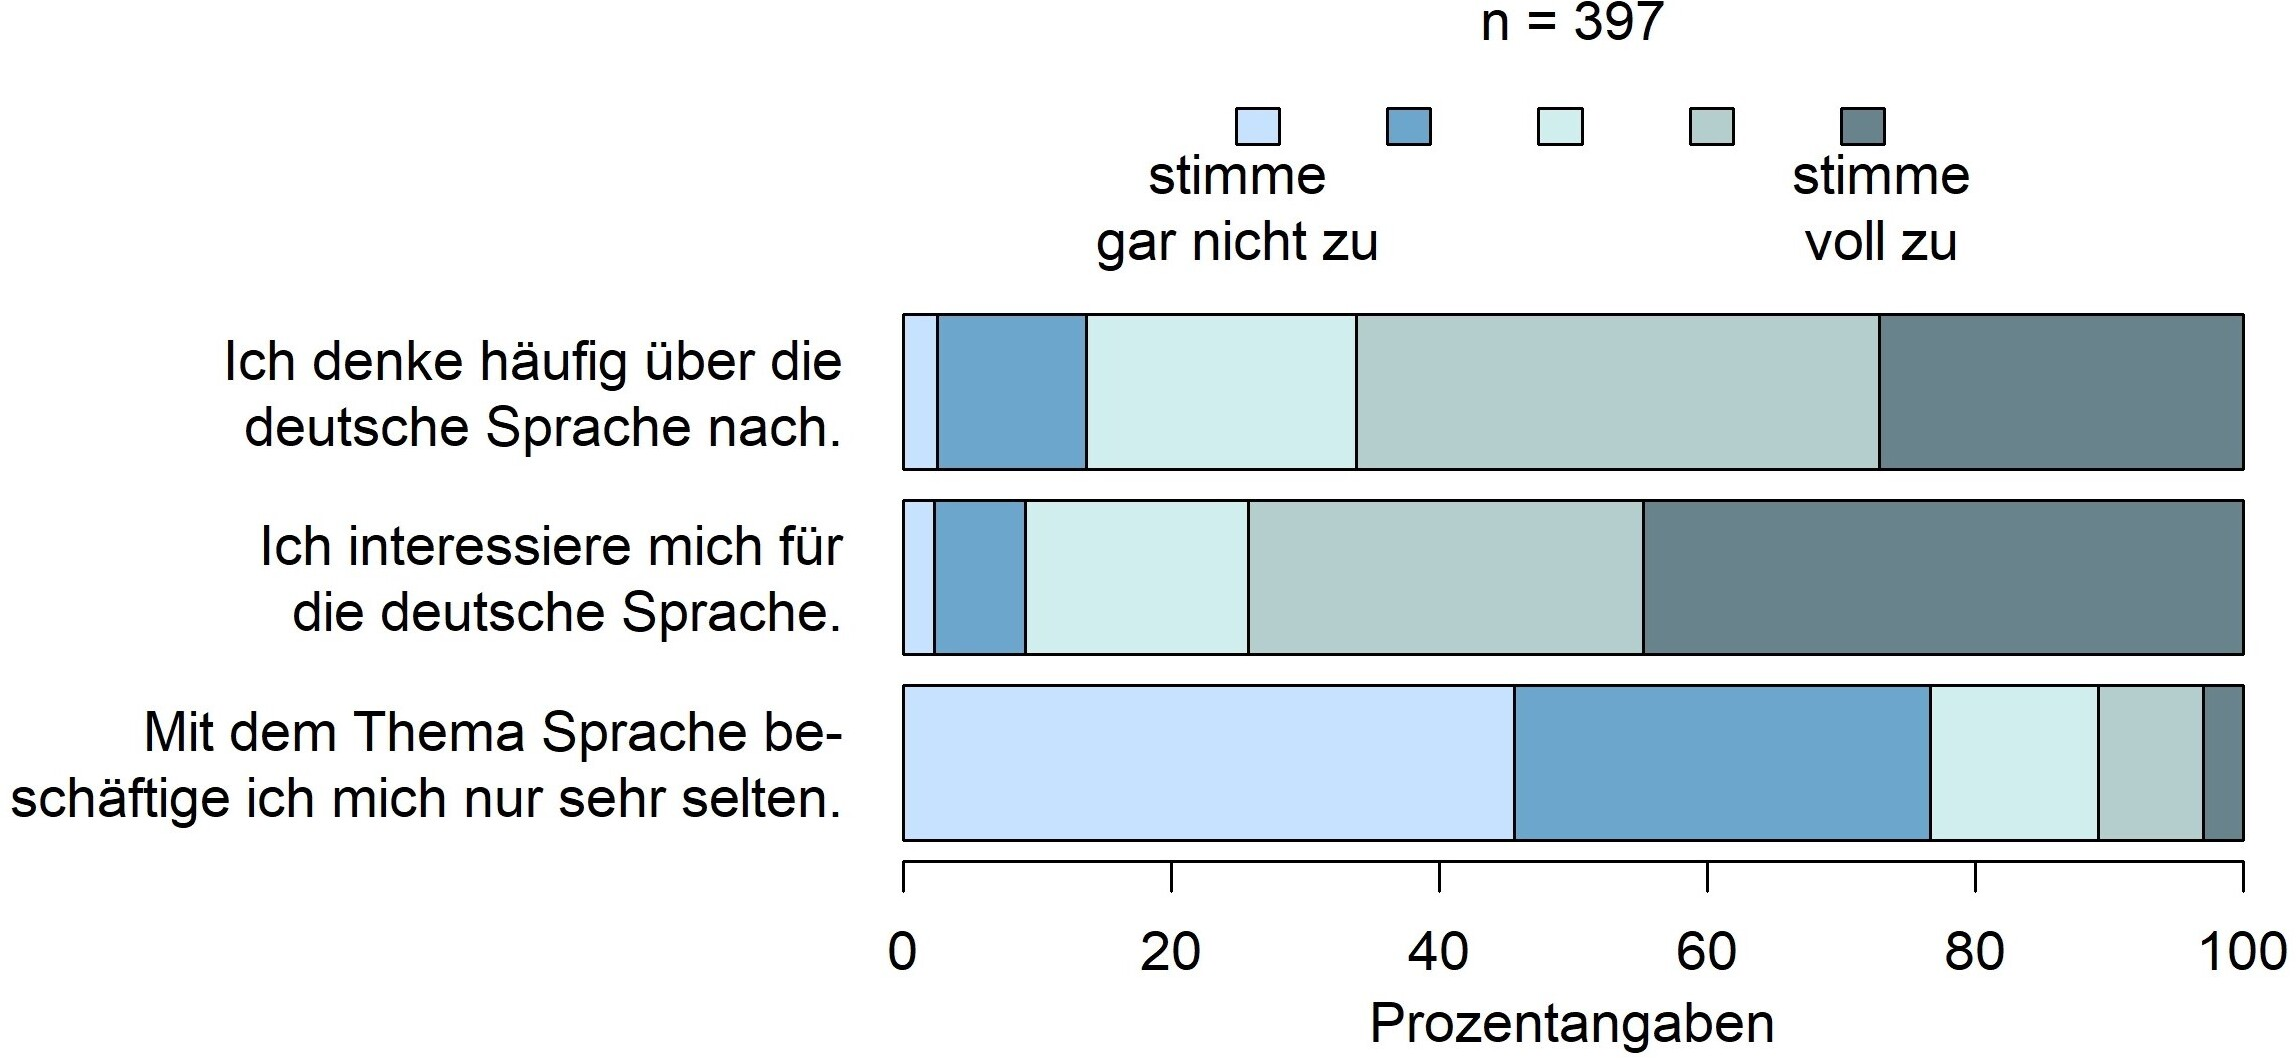
\includegraphics[width=\textwidth]{Sprachbewusstheit.jpg}
\caption{Beantwortung der Likert-Items zur Sprachbewusstheit}
\label{pic:SB}
\end{figure}
 
Zwei Drittel der Befragten stimmen der Aussage zu, häufig über die deutsche Sprache nachzudenken. 
Noch etwas mehr (ungefähr drei Viertel) stimmen zu, dass sie sich für die deutsche Sprache interessieren. 
Die Aussage, dass sie sich nur sehr selten mit dem Thema Sprache beschäftigen, verneinen beinahe 80~\%. 
Dass an der Umfrage vor allem sprachinteressierte Personen teilnahmen, liegt mit Sicherheit in erster Linie daran, dass sie als Umfrage zu einem sprachbezogenen Thema angekündigt wurde. 
\subsection{Selbsteinschätzung der Sprachsicherheit der Befragten}
\label{sec:Sprachsicherheit}
Die meisten TeilnehmerInnen schätzen nicht nur ihr Interesse für Sprache, sondern auch ihre sprachliche Sicherheit recht hoch ein, wie \autoref{pic:SK} zeigt (s. zusätzlich \autoref{table:LikertZsfsgAnh} im Anhang). 
Die Likertskala zu diesem Aspekt fragt insbesondere ab, wie die eigenen Kompetenzen im Bereich Grammatik und Rechtschreibung eingestuft werden. 
Sie besteht aus folgenden drei Aussagen: 
\begin{enumerate}
\item Ich bin bei sprachlichen Fragen häufig unsicher.
\item Wenn jemand eine Frage zu Grammatik oder Rechtschreibung hat, kann ich meistens weiterhelfen.
\item  Ich kenne mich gut mit der deutschen Grammatik aus.
\end{enumerate}

Nur 6,5~\% der Befragten stimmen der Aussage zu, sich bei sprachlichen Fragen häufig unsicher zu fühlen. 
80~\% meinen, Fragen zu Grammatik und Rechtschreibung meist beantworten zu können und 75~\% geben an, sich gut mit der Grammatik auszukennen. 
8 bzw. 7~\% stimmen den Aussagen nicht zu, dass sie sich mit der Grammatik auskennen bzw. bei sprachlichen Fragen weiterhelfen können. 
An der Studie nahmen also durchaus auch Personen teil, die ihr Wissen über Grammatik und Rechtschreibung als gering einschätzen, diese sind allerdings in der Unterzahl.
\begin{figure}[htb]
\centering
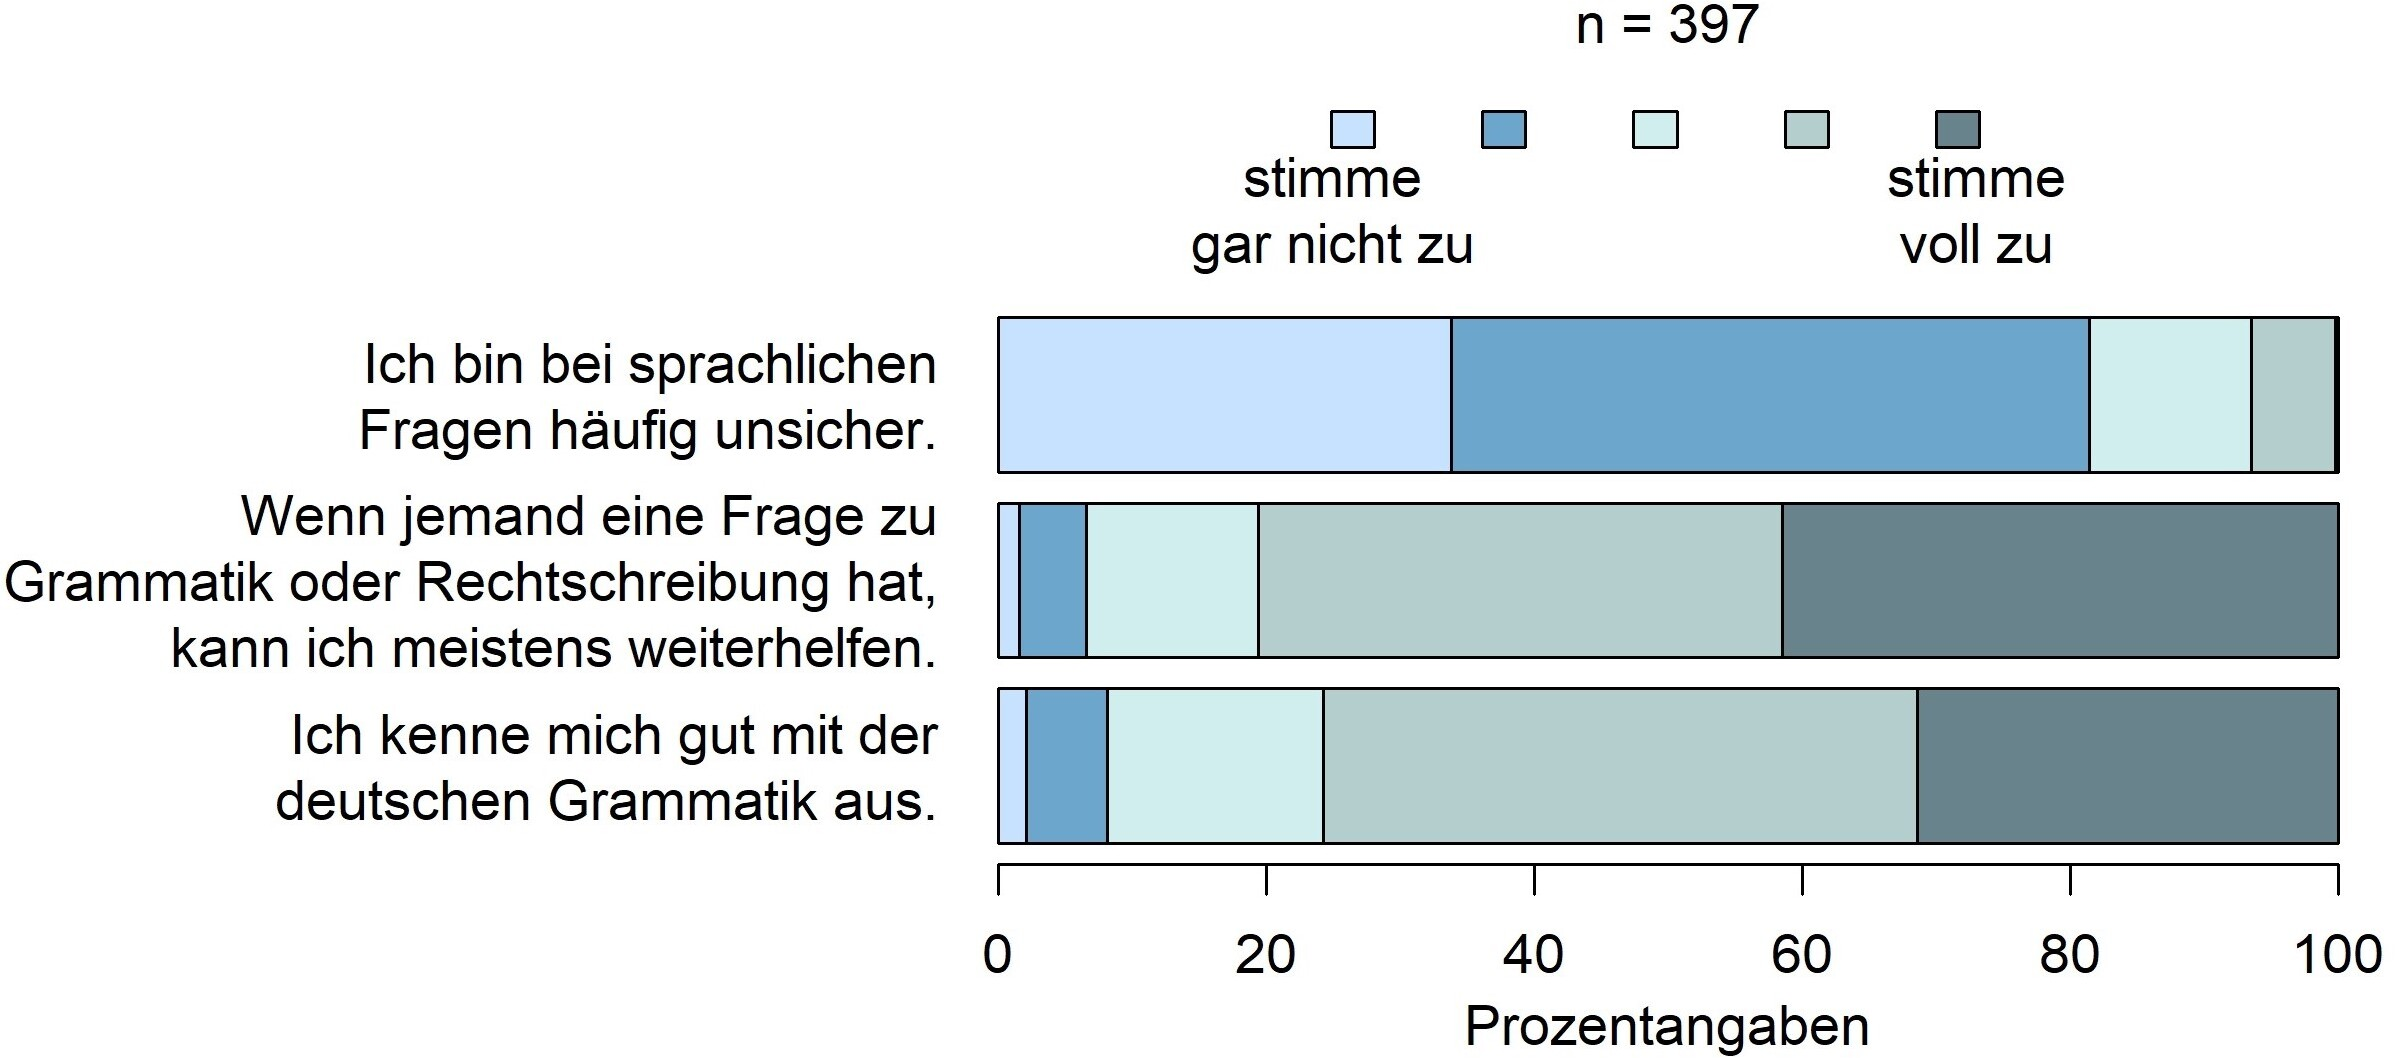
\includegraphics[width=\textwidth]{Sprachkompetenz.jpg}
\caption{Beantwortung der Likert-Items zur Sprachsicherheit}
\label{pic:SK}
\end{figure}

Um zu überprüfuen, inwiefern sich die Selbsteinschätzung der eigenen Sprachsicherheit auf die Angaben im Akzeptabilitätstest und im Produktionsexperiment auswirkt, können die Befragten in zwei Gruppen aufgeteilt werden: 
diejenigen, die ihre sprachliche Sicherheit hoch einschätzen, und diejenigen, die ihre sprachliche Sicherheit gering einschätzen. 
Hierfür muss zunächst das negative Item der Likertskala zur Sprachsicherheit, \glqq ich bin bei sprachlichen Fragen häufig unsicher\grqq, umgepolt werden. 
Die Umpolung hat zur Folge, dass ein hoher Zustimmungswert auch bei diesem Item als Hinweis auf eine hohe Einschätzung der eigenen sprachlichen Sicherheit gedeutet werden kann (\autoref{sec:RE}). 
Anschließend kann der Mittelwert der Zustimmung zu den drei Items der Skala gebildet werden, an dem abgelesen werden kann, wie stark eine befragte Person der Skala insgesamt zustimmt. 
Befragte mit durchschnittlichen Zustimmungswerten von über drei bilden die Gruppe derer, die ihre Sprachsicherheit hoch einschätzen (abgekürzt mit Ss+). 
Befragte mit Durchschnittswerten von drei oder weniger bilden die Gruppe derer, die ihre Sprachsicherheit gering einschätzen (abgekürzt mit Ss--). 
In der Gruppe Ss+ befinden sich 344 Befragte, in der Gruppe Ss-- nur 53. 

Wichtig ist, dass mit der Likertskala die Selbsteinschätzung der Befragten gemessen wird, nicht ihre tatsächliche Sicherheit. 
Dass es hier Diskrepanzen geben kann, zeigt etwa eine Studie von \citet{Gartig2010}:
Hier schätzten auch Befragte, die in einem Rechtschreibtest schlecht abschnitten, ihre eigenen Deutschkenntnisse größtenteils als gut oder sehr gut ein \citep[s.][12--13]{Gartig2010}. 

Die Selbsteinschätzung der sprachlichen Sicherheit korreliert zu einem gewissen Grad mit der in \autoref{sec:Beruf} thematisierten Textaffinität des Berufs. 
Wie \autoref{table:SprachwissenundBeruf} zeigt, ist der Anteil an Befragten mit einem textaffinen Beruf unter denen, die ihre Sprachsicherheit hoch einschätzen, höher als unter denen, die ihre Sprachsicherheit gering einschätzen. 
Jedoch hat auch rund die Hälfte der Personen, die ihre Kompetenzen im Bereich Grammatik und Rechtschreibung gering einschätzen, im Beruf häufig oder täglich mit längeren Texten zu tun. 

\begin{table}
\centering
\begin{tabular}{lrrrr}
\multicolumn{1}{c}{\textbf{}} & Sprachsicherheit hoch eingeschätzt & Sprachsicherheit gering eingeschätzt \\
\midrule
Beruf textaffin               & 255                                             & (74 \%)                                             & 28                                               & (53 \%)                                               \\
Beruf nicht textaffin         & 89                                              & (26 \%)                                             & 25                                               & (47 \%)                                               \\
gesamt                        & 344                                             & (100 \%)                                            & 53                                               & (100 \%)                                              \\ 
\end{tabular}
\caption{Zusammenhang zwischen der Selbsteinschätzung der Sprachsicherheit und der Textaffinität des Berufs}
\label{table:SprachwissenundBeruf}
\end{table}

% Änderung Anfang
Bezogen auf die gesamte Befragtengruppe lässt sich damit festhalten, dass 64 \% der TeilnehmerInnen ihre Sprachsicherheit hoch einschätzen und einen textaffinen Beruf ausüben, während 22 \% aller Befragten ihre Sprachsicherheit hoch einschätzen, ohne einen textaffinen Beruf zu haben.
7 \% der Befragten schätzen die eigene Sprachsicherheit gering ein und gehen einem textaffinen Beruf nach, 6 \% hingegen schätzen die eigene Sprachsicherheit gering ein und haben keinen textaffinen Beruf. %Änderung Ende
\subsection{Variationstoleranz der Befragten}
\label{sec:Variationstoleranz}
Die Likertskala zur Einstellung gegenüber Variation zielt darauf ab, herauszufinden, inwiefern die Befragten verschiedene Aspekte der Standardsprachideologie und der Sprachverfallsideologie vertreten, wie etwa die Auffassung, dass nur eine Variante korrekt sein kann (s. \autoref{pic:VT}, vgl. \autoref{sec:MetapragmatikVariationWandel}). 
Sie enthält folgende vier Aussagen: 
\begin{enumerate}
\item Je nach Region können verschiedene Sprachformen richtig sein. 
\item Es ist gut, dass sich der Duden dem aktuellen Sprachgebrauch anpasst.
\item In der Sprache sollten feste Regeln vorschreiben, was richtig und was falsch ist. 
\item Die deutsche Grammatik verfällt immer mehr. 
\end{enumerate}

\begin{figure}[htb]
\centering
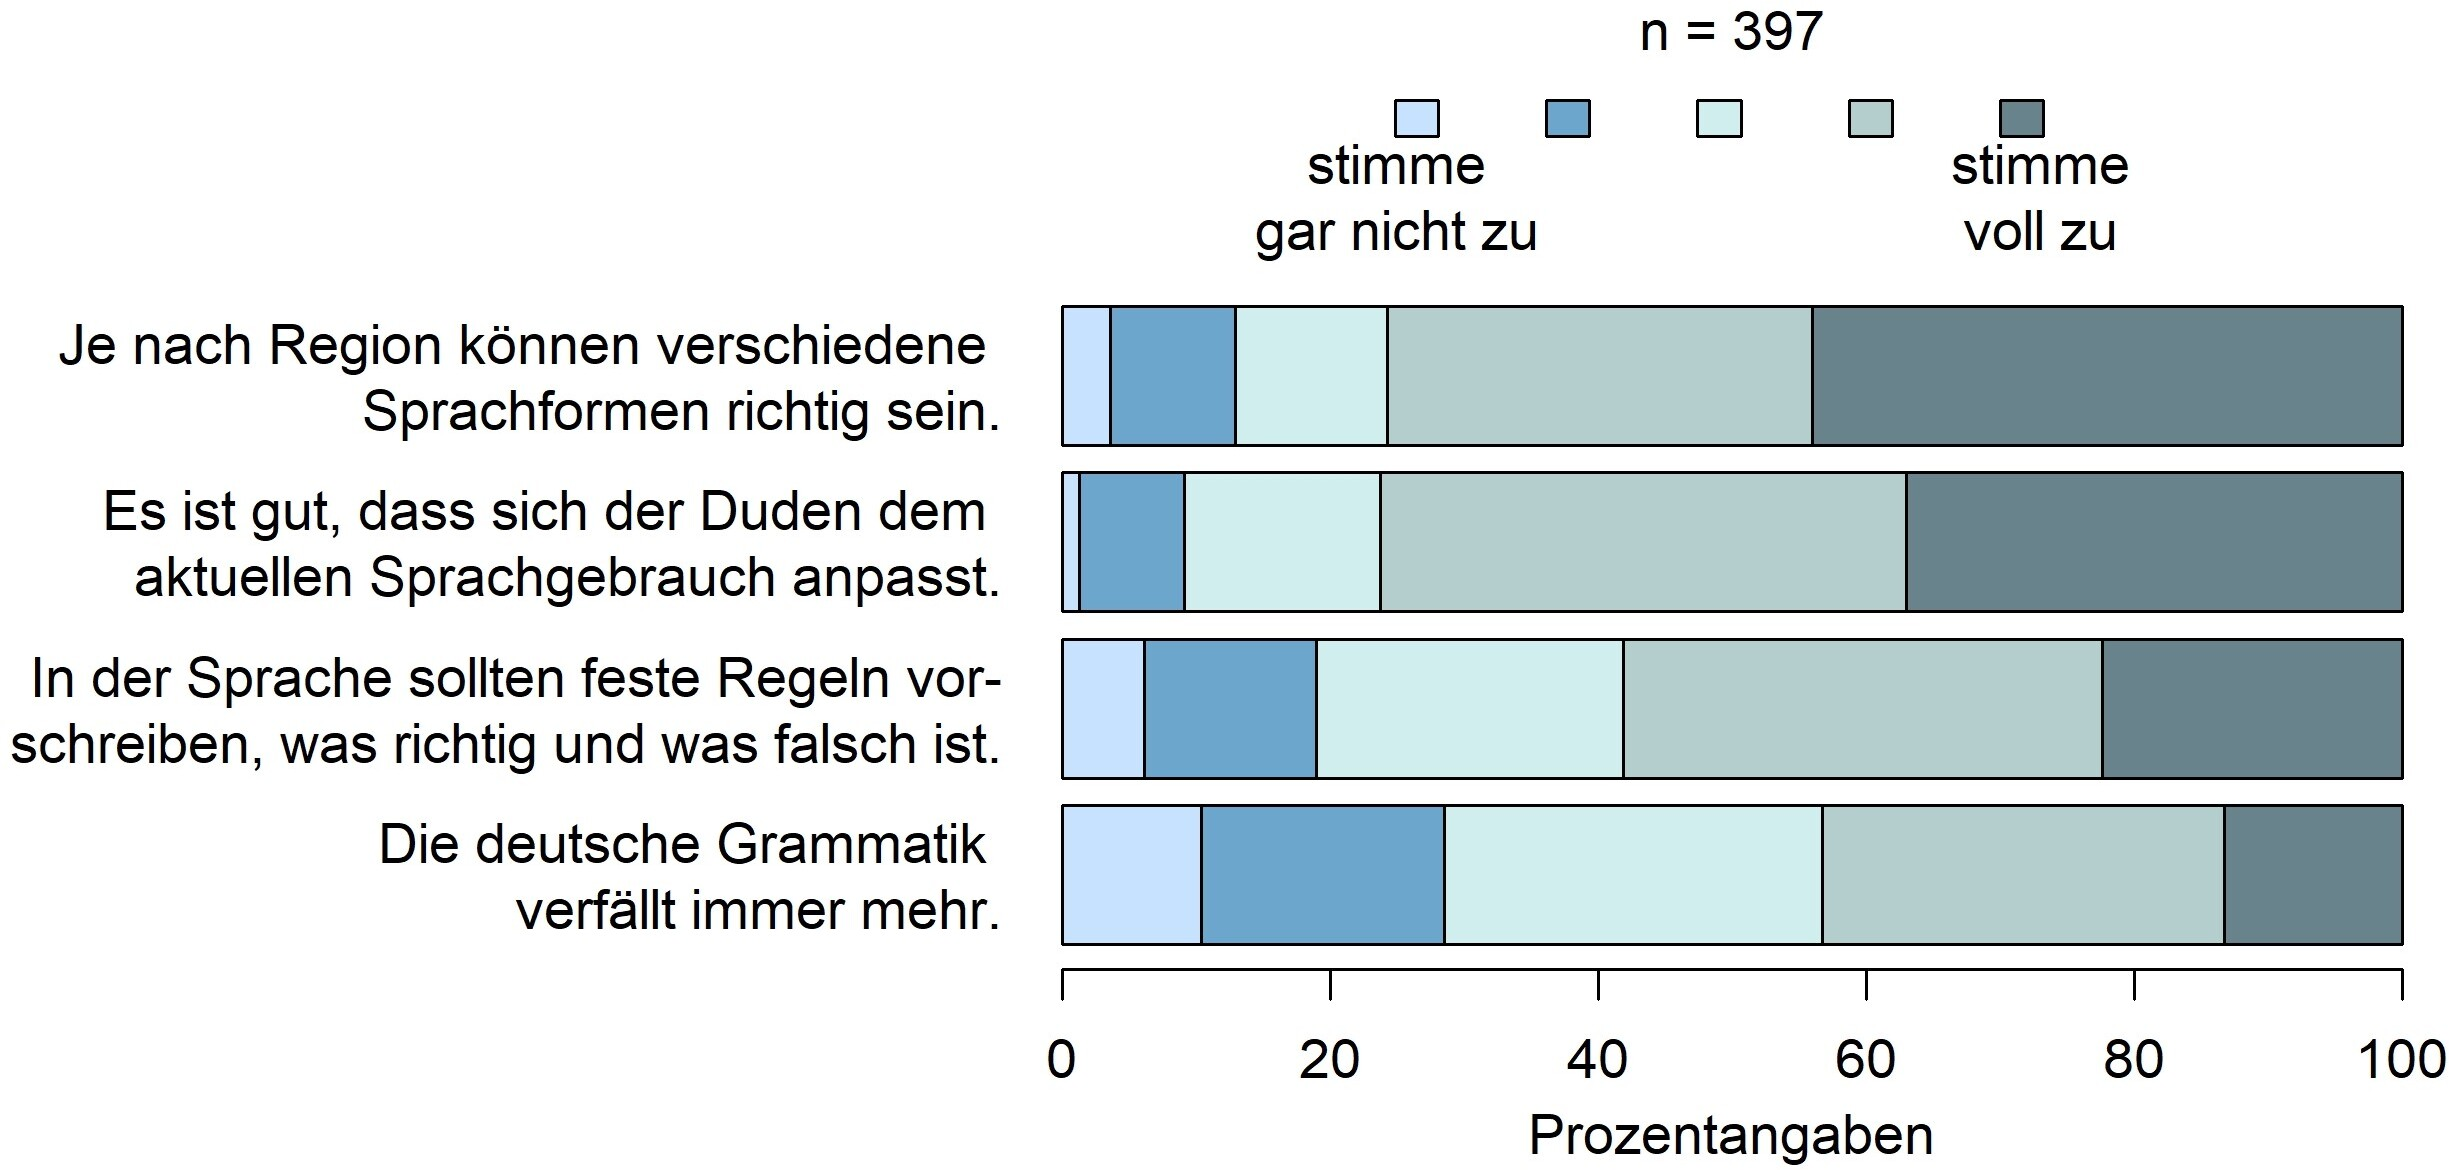
\includegraphics[width=\textwidth]{Variationstoleranz.jpg}
\caption{Beantwortung der Likert-Items zur Variationstoleranz}
\label{pic:VT}
\end{figure}

Hier zeigt sich auf der einen Seite eine Toleranz gegenüber regionaler sowie diachroner Variation: Rund drei Viertel der Befragten stimmen zu, dass je nach Region verschiedene sprachliche Formen richtig sein können (für die genauen Zahlen s. auch \autoref{table:LikertZsfsgAnh} im Anhang). Beinahe ebenso viele befürworten, dass der Duden sich dem aktuellen Sprachgebrauch anpasst. 
Auf der anderen Seite zeigen sich aber auch der Wunsch nach präskriptiven Regeln und die Vorstellung, die Sprache verfalle: 58~\% der Befragten stimmen der Aussage zu, feste Regeln sollten in der Sprache vorschreiben, was richtig und was falsch ist. 
43~\% finden, dass die deutsche Grammatik immer mehr verfällt.
Die Ideologie der sprachlichen Einheitlichkeit und die Vorstellung eines drohenden Verlusts dieser Einheitlichkeit sind unter den Befragten also recht verbreitet. 

Für die Analyse von Zusammenhängen zwischen der Variationstoleranz der Befragten und ihren Angaben im Akzeptabilitätstest sowie ihrer Kasuswahl können zwei Gruppen gebildet werden.
Hierfür werden wieder zunächst die negativen Items der Likertskala zur Variationstoleranz umgepolt, sodass ein hoher Zustimmungswert bei allen Items für eine hohe Zustimmung zu Variation steht (\autoref{sec:RE}). 
Die Items, die dafür umgepolt werden müssen, sind \glqq in der Sprache sollten feste Regeln vorschreiben, was richtig und was falsch ist\grqq{} und \glqq die deutsche Grammatik verfällt immer mehr\grqq.
Befragte, die auf der Likertskala zur Variationstoleranz einen durchschnittlichen Wert von drei oder weniger erzielen, bilden die wenig variationstolerante Gruppe, im Folgenden abgekürzt mit Vt--. 
Diese Gruppe besteht aus insgesamt 169 Befragten. 
Befragte mit Likertwerten von über drei bilden die variationstolerante Gruppe, im Folgenden abgekürzt mit Vt+. 
Diese Gruppe umfasst 228 Befragte. 
Beide Gruppen unterscheiden sich kaum, was ihre Zusammensetzung nach soziodemografischen Merkmalen wie Alter, regionale Herkunft oder Bildungsstand angeht (s. \autoref{table:AnhAlterundVt} bis \autoref{table:AnhBildungundVt} im Anhang). 
Alle Differenzen liegen im einstelligen Prozentbereich. 
\subsection{Zusammenfassung zur Zusammensetzung der Befragtengruppe}
\label{sec:ZsfsgBefragte}
Die soziodemografischen Angaben der Befragten lassen sich wie folgt zusammenfassen:
Die TeilnehmerInnen der Studie sind überwiegend jung und weiblich, stammen aus Norddeutschland, sprechen keinen Dialekt, verfügen über einen hohen Bildungsabschluss und üben einen Beruf aus, in dem sie häufig mit längeren Texten zu tun haben.
Teilweise gibt es Überschneidungen zwischen den soziodemografischen Merkmalen. 
So finden sich in der Gruppe der 18- bis 25-Jährigen besonders viele weibliche Befragte. 
Unter den über 60-Jährigen ist der Anteil an Befragten aus Norddeutschland und an Befragten ohne Hochschulabschluss höher als in anderen Altersgruppen. 
DialektsprecherInnen finden sich vor allem unter Befragten aus süddeutschen Bundesländern. 

\autoref{pic:Likertskalen} fasst die Ergebnisse der Likertskalen zu Sprachbewusstheit, Sprachsicherheit und Variationstoleranz zusammen. 
Dargestellt sind die Likertwerte aller Befragten für die drei Skalen. 
Für jede befragte Person sind also drei Werte abgebildet, die jeweils  dem Durchschnitt der Zustimmung zu den einzelnen Items einer Skala entsprechen.
Die Aussagen, bei denen Zustimmung bedeutet, dass das abgefragte Konzept wenig ausgeprägt ist, werden zur Berechnung dieser Durchschnittswerte zuvor umgepolt, wie  in \autoref{sec:RE} beschrieben. 
Ein Beispiel für ein solches Item ist die dritte Aussage auf der Likertskala zur Sprachbewusstheit (\glqq mit dem Thema Sprache beschäftige ich mich nur sehr selten\grqq).
Wenn eine Person also bspw. auf der Likertskala zur Sprachbewusstheit den ersten beiden Items voll zustimmt und dem dritten Item gar nicht zustimmt, so erhält sie für die Sprachbewusstheit den Wert 5. 
\begin{figure}
\centering
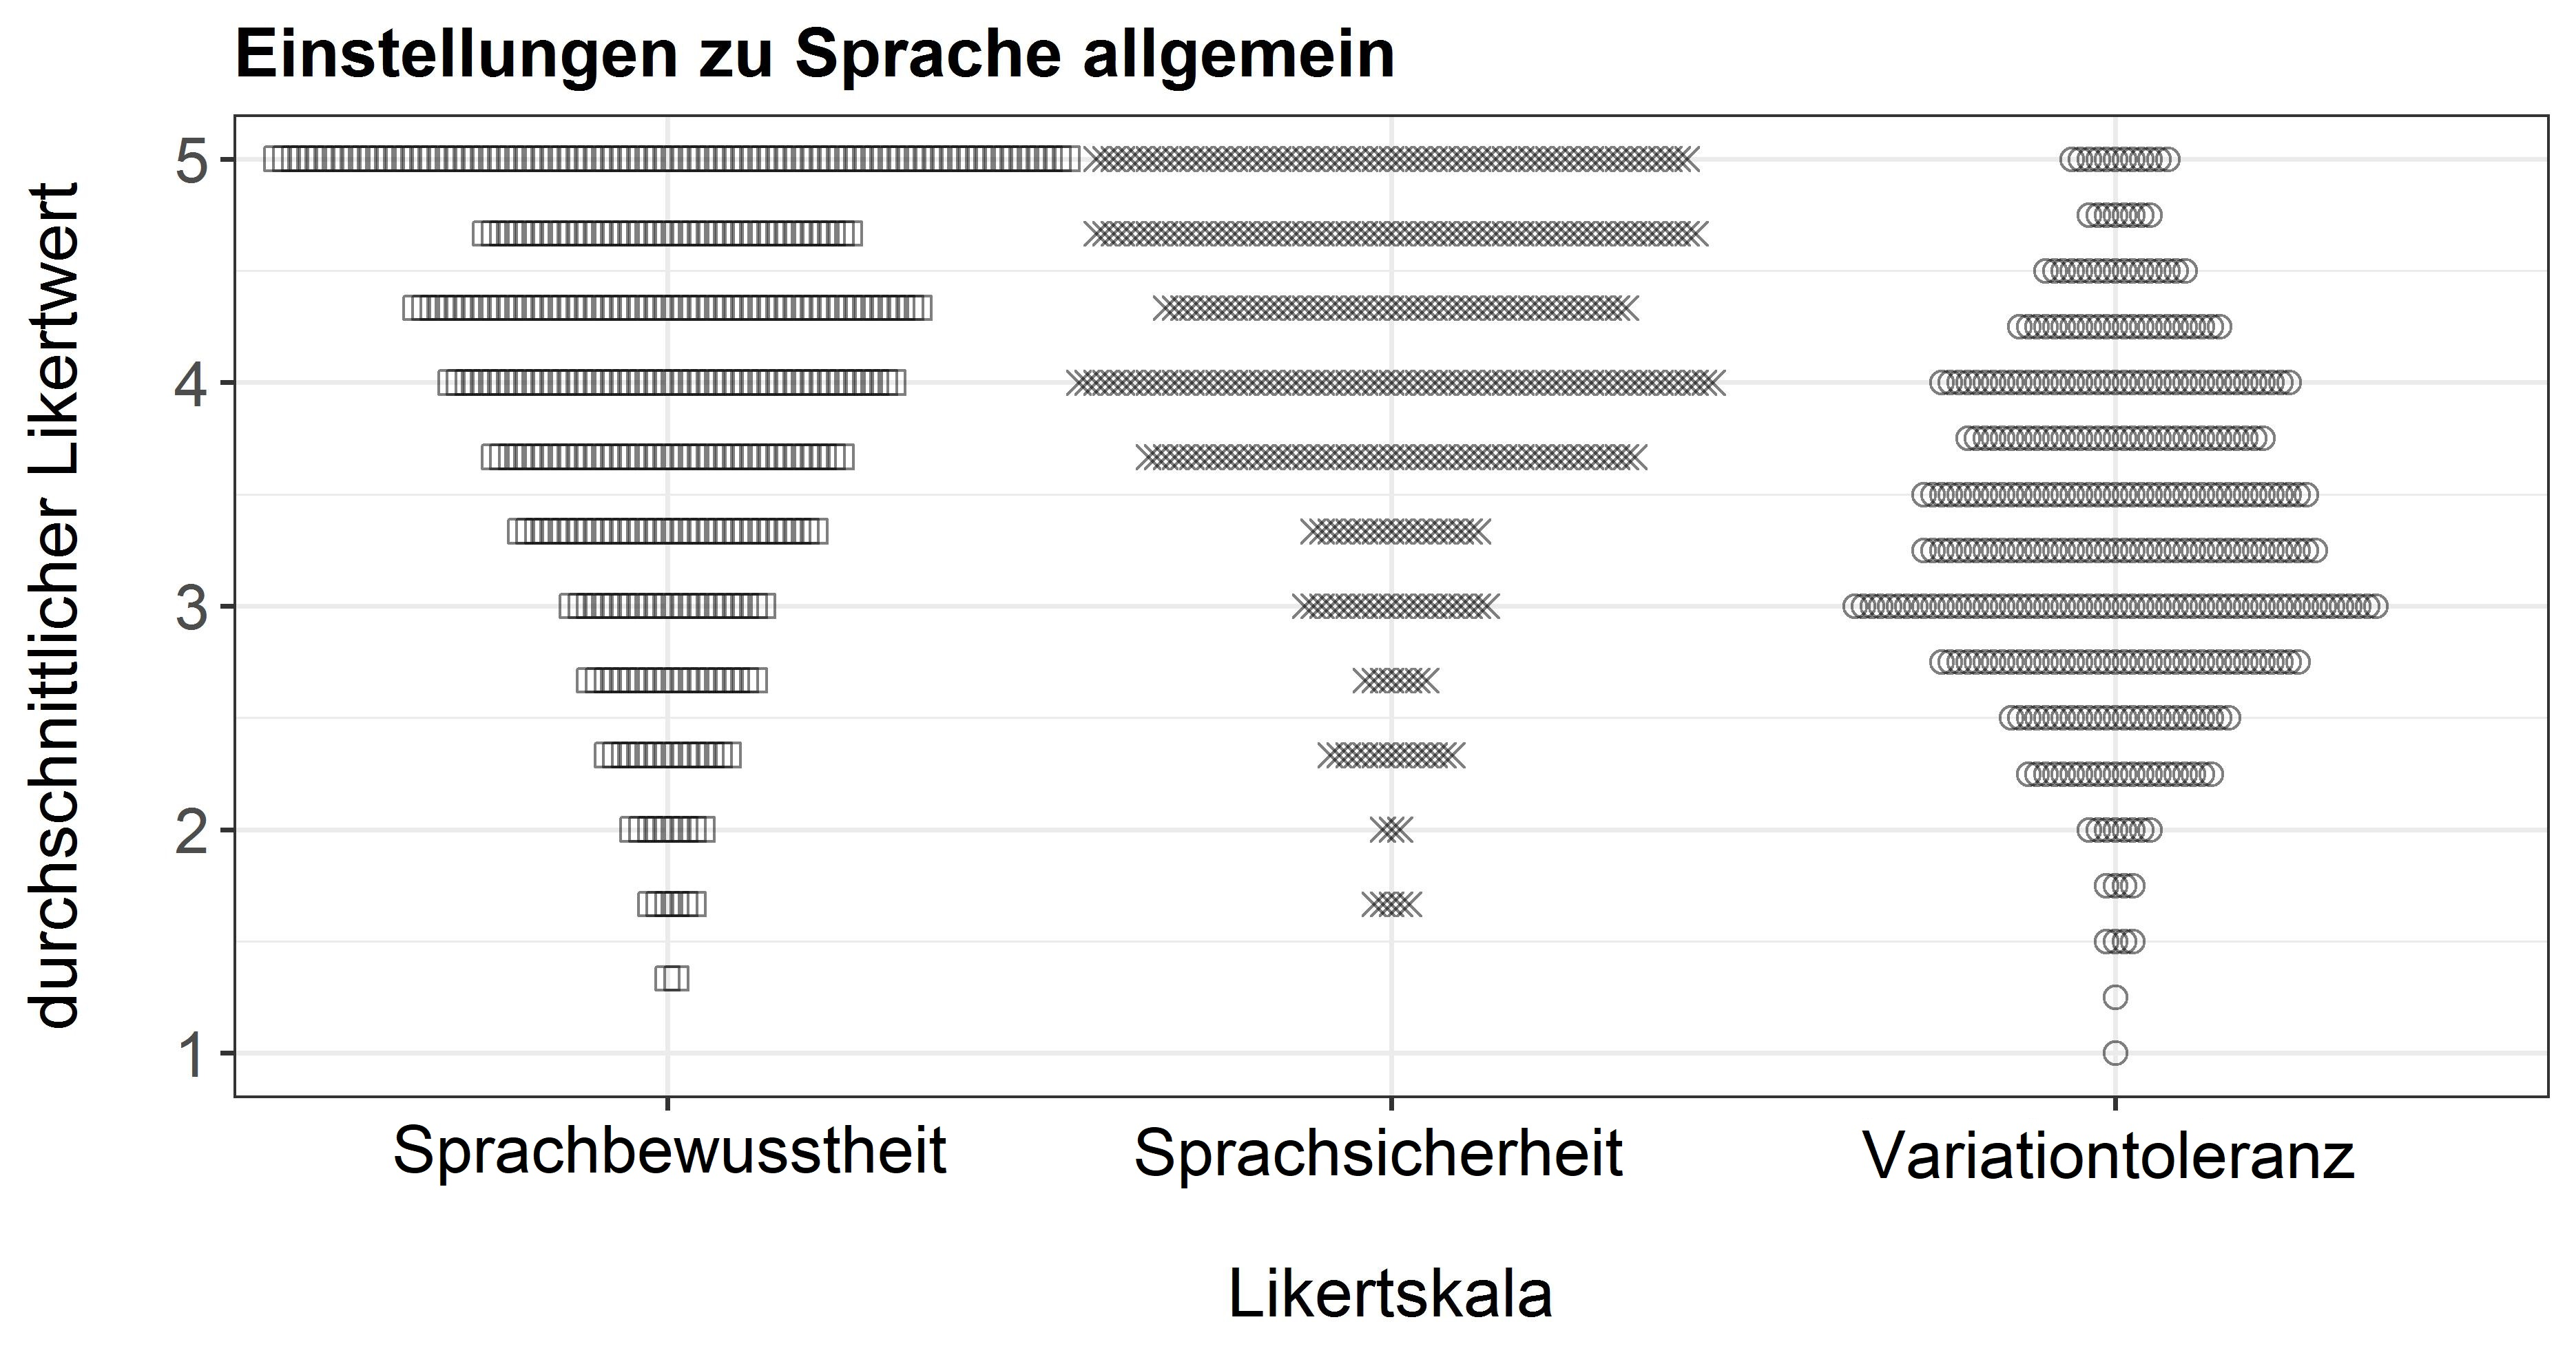
\includegraphics[width=\textwidth]{likertbee.jpg}
\caption{Likertwerte der Befragten zu Sprachbewusstheit, Sprachsicherheit und Variationstoleranz}
\label{pic:Likertskalen}
\end{figure}
 
An den durchschnittlichen Likertwerten lässt sich zusammenfassend ablesen, dass das Interesse an Sprache sowie die Einschätzung der eigenen Sprachsicherheit unter den Befragten recht hoch sind:
Auf den Skalen zu Sprachbewusstheit und Sprachsicherheit erreichen die meisten Befragten hohe durchschnittliche Likertwerte zwischen 4,0 und 5,0. 
Nur wenige Befragte haben hier durchschnittliche Likertwerte von unter 3,0. 
Die Toleranz für sprachliche Variation liegt hingegen bei den meisten Befragten im mittleren Bereich. 
Auch hier finden sich jedoch mehr hohe als niedrige Durchschnittswerte, was auf eine insgesamt eher hohe Variationstoleranz in der Befragtengruppe hindeutet.  
\section{Assoziationen zu den Rektionsvarianten}
\label{sec:ErgAss}
Im Assoziationsteil des Fragebogens wurden explizite metapragmatische Äußerungen zu den Rektionsvarianten von \wegen, \waehrend, \dank{} und \gegenueber{} erhoben. 
Sie wurden einerseits mithilfe von semantischen Differenzialen erfragt und andererseits mithilfe von offenen Fragen nach Assoziationen. 
Für diesen Teil des Fragebogens wurden die Befragten auf vier Gruppen aufgeteilt. 
In jeder Gruppe wurden Assoziationen zu beiden Rektionsvarianten einer der untersuchten Präpositionen erhoben (\autoref{sec:Ass}).
\autoref{table:Ass} gibt einen Überblick über die jeweiligen Beispielsätze und die Anzahl der Befragten pro Gruppe. 

\begin{table}
\centering
\begin{tabular}{llr}
\lsptoprule
Präposition & Beispielsätze im Fragebogen                                                                                                               & \multicolumn{1}{l}{Befragte} \\
\midrule
\textit{dank}        & \textit{\begin{tabular}[c]{@{}l@{}}Dank des Brückentags konnte ich ihn besuchen. \\ Dank dem Brückentag konnte ich ihn besuchen.\end{tabular}}     & 96                                                         \\ \tablevspace
\textit{gegenüber}   & \textit{\begin{tabular}[c]{@{}l@{}}Sie hat es gegenüber des Lehrers nicht erwähnt. \\ Sie hat es gegenüber dem Lehrer nicht erwähnt.\end{tabular}} & 101                                                        \\ \tablevspace
\textit{wegen}       & \textit{\begin{tabular}[c]{@{}l@{}}Ich bin wegen dem Starkregen zu spät gekommen.\\ Ich bin wegen des Starkregens zu spät gekommen.\end{tabular}}  & 96                                                         \\ \tablevspace
\textit{während}     & \textit{\begin{tabular}[c]{@{}l@{}}Während dem Telefonat mache ich Notizen. \\ Während des Telefonats mache ich Notizen.\end{tabular}}             & 104                                                        \\ 
\lspbottomrule
\end{tabular}
\caption{Beispielsätze und Anzahl der Befragten in den vier Gruppen im Assoziationstest}
\label{table:Ass}
\end{table}
Im Folgenden werden zunächst die Ergebnisse der semantischen Differenziale dargestellt. 
Die anschließenden Abschnitte wenden sich den freien Assoziationen zu.
\subsection{Ergebnisse der semantischen Differenziale}
\label{sec:ErgSemDiff}
Mithilfe der semantischen Differenziale wurde abgefragt, inwiefern die Befragten die präsentierten Varianten als gebildet, kompetent, freundlich und sympathisch empfinden. 
Hierfür konnten die Befragten die beiden in ihrer Gruppe abgefragten Varianten jeweils auf einer fünfstufigen Skala bewerten. 
An einem Ende der Skala stand etwa \glqq ungebildet\grqq, am anderen \glqq gebildet\grqq{} (\autoref{sec:Ass}). 
%Die Angabe eines Mittelwerts bei Skalen mit nur einem einzelnen Item ist zwar problematisch, in der Spracheinstellungsforschung aber durchaus üblich \citep[vgl. etwa][184]{Plewnia.2011}. 
%Um die Ergebnisse der Studie mit anderen vergleichbar zu machen, wird daher auch hier auf diese Darstellung zurückgegriffen. 
Die Ergebnisse der semantischen Differenziale sind in \autoref{pic:sdsWegen} bis \autoref{pic:sdsGegenueber} in Form von Boxplots dargestellt.
In den Boxplots ist jeweils der Median für die Einschätzung der Varianten auf der semantischen Differenzialskala als fettgedruckte Linie eingezeichnet. 
Zusätzlich sind die Quartile abzulesen: Das untere Ende einer Box entspricht jeweils dem ersten Quartil, das obere Ende dem dritten. 
Das heißt, es liegen jeweils 25~\% der Daten unter dem unteren Rand einer Box und 75~\% unter dem oberen Rand der Box.
Die Spanne der Box entspricht dem Interquartilsabstand (IQR). 
Die Whiskers reichen jeweils bis zu dem Wert in den Daten, der sich noch innerhalb des 1,5-fachen Interquartilsabstands befindet.
Im Folgenden werden zunächst die Ergebnisse zu den Genitivpräpositionen \wegen{} und \waehrend{} besprochen und anschließend die Ergebnisse zu den Dativpräpositionen \dank{} und \gegenueber. 

Betrachtet man die beiden ursprünglichen Genitivpräpositionen \wegen{} und \waehrend{} (s. \autoref{pic:sdsWegen} und \autoref{pic:sdsWaehrend}), fällt zweierlei auf: 
Erstens wird die Genitivrektion in den Statuskategorien \glqq Bildung\grqq{} und \glqq Kompetenz\grqq{} deutlich positiver bewertet als die Dativrektion. 
\object{Während} mit dem Genitiv wird sogar von allen Befragten mit mindestens dem Wert 3 auf der Skala zwischen ungebildet und gebildet bewertet. 
Hinzu kommt, dass die Einschätzung der Bildung bei \waehrend{} plus Dativ der einzige Fall in den semantischen Differenzialen ist, bei dem der höchste Wert, 5, nicht vergeben wurde (s. auch \autoref{table:sdswaehrendAnh} im Anhang). 
VerwenderInnen der Dativrektion bei \waehrend{} werden also von niemandem für sehr gebildet gehalten. 
Zweitens unterscheidet sich die Bewertung der beiden Rektionsvarianten in den Wärmekategorien jeweils kaum.
\begin{figure}
\centering
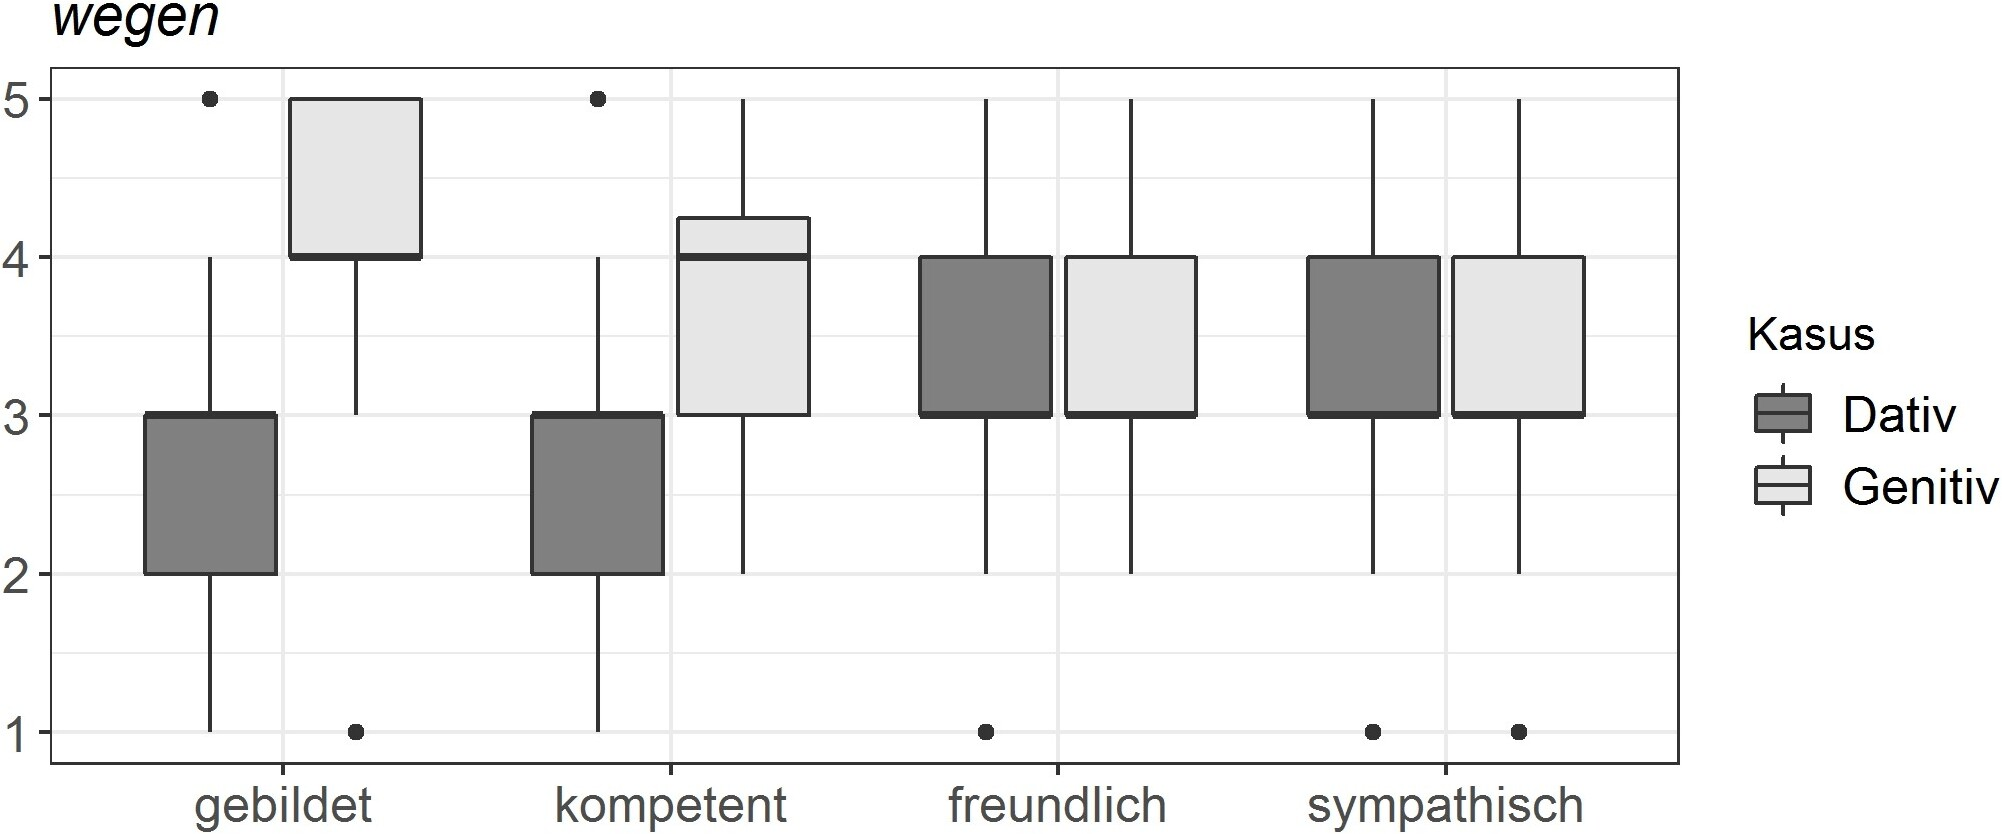
\includegraphics[width=\textwidth]{sdswegenBoxplots.jpg}
\caption{Bewertung der Rektionsvarianten von \wegen}
\label{pic:sdsWegen}
\end{figure}
\begin{figure}
\centering
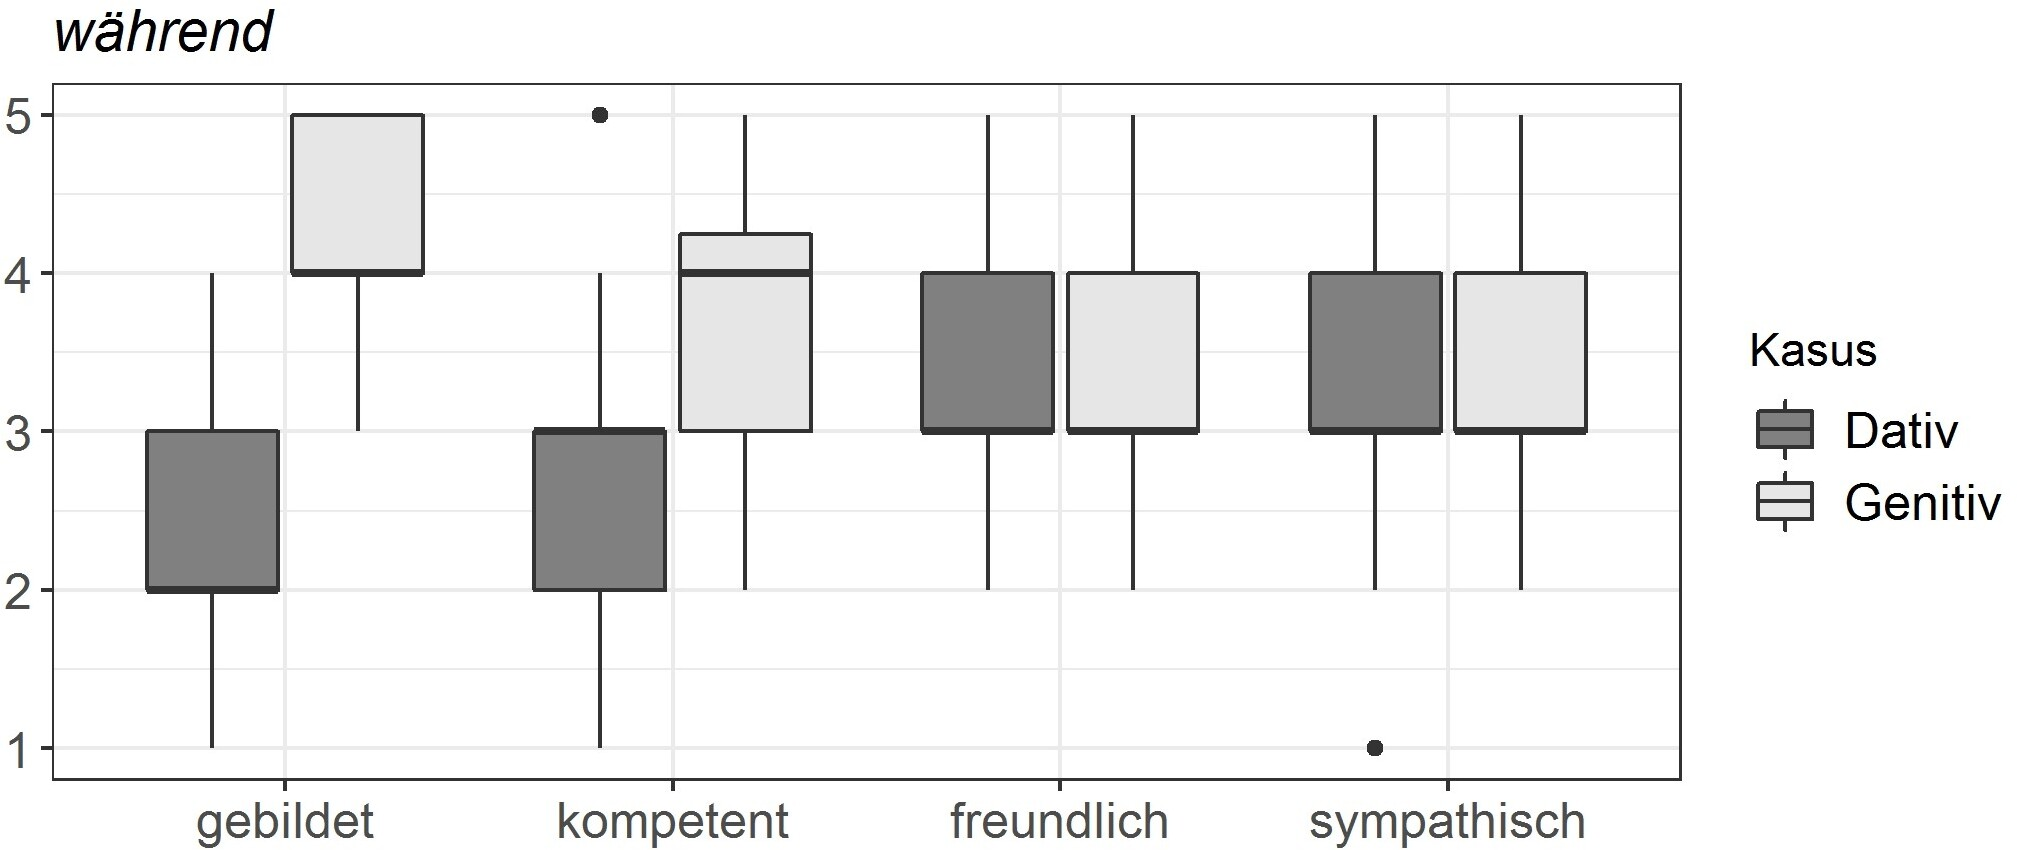
\includegraphics[width=\textwidth]{sdswaehrendBoxplots.jpg}
\caption{Bewertung der Rektionsvarianten von \waehrend}
\label{pic:sdsWaehrend}
\end{figure}
 
In \autoref{pic:sdsDank} ist erkennbar, dass der Genitiv bei \dank{} stark mit den Statuskategorien in Verbindung gebracht wird: 
Der Median liegt sowohl in der Kategorie \glqq Bildung\grqq{} als auch in der Kategorie \glqq Kompetenz\grqq{} bei 5.
Das heißt, mindestens die Hälfte der Befragten hat \dank{} plus Genitiv mit 5, also als sehr gebildet bzw. sehr kompetent bewertet.
\begin{figure}
\centering
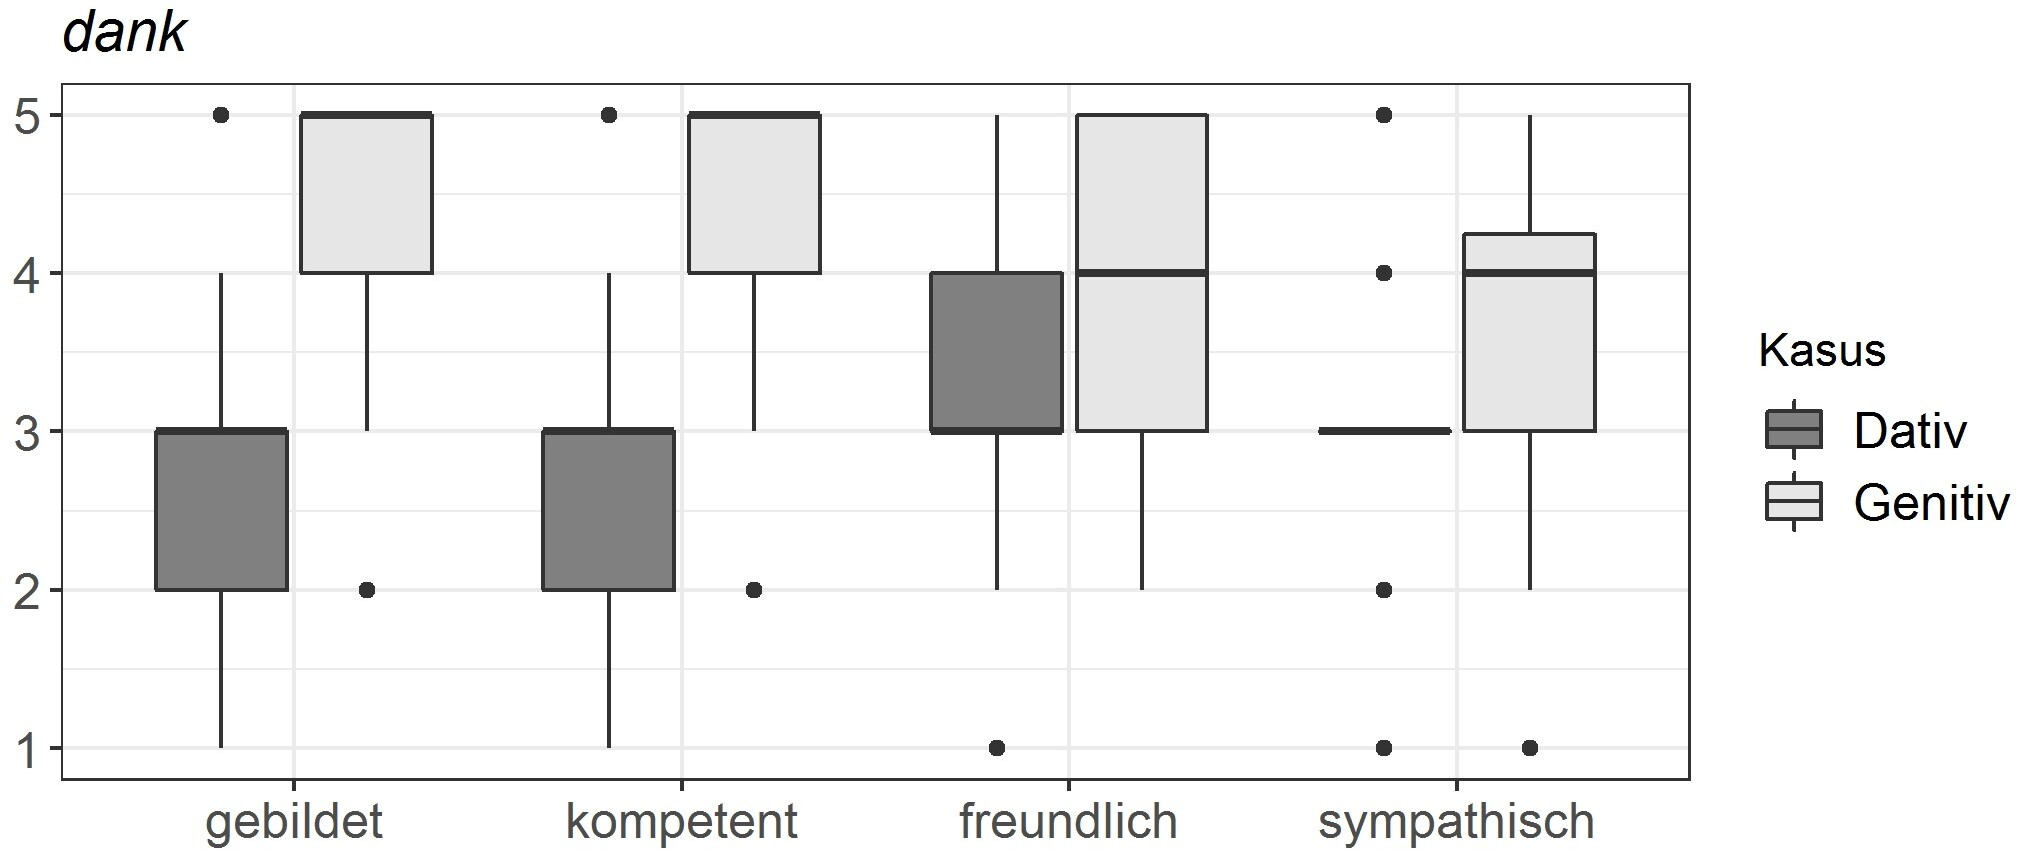
\includegraphics[width=\textwidth]{sdsdankBoxplots.jpg}
\caption{Bewertung der Rektionsvarianten von \dank}
\label{pic:sdsDank}
\end{figure}

Bei der Bewertung von \dank{} plus Genitiv als gebildet und kompetent scheint es außerdem eine hohe Einigkeit unter den Befragten zu geben, was sich darin zeigt, dass das untere Quartil jeweils bei 4 liegt. 
Der Großteil der Gruppe, die die Rektionsvarianten von \dank{} bewertete, hat in den Statuskategorien für die Genitivrektion also einen der beiden höchsten Werte gewählt: 
Auf der Skala für die Kategorie Bildung kreuzten insgesamt 87 von 96 Befragten 4 oder 5 an, auf der Skala für die Kategorie Kompetenz waren es 78 (s. \autoref{table:sdsdankAnh} im Anhang). 
Gleichzeitig wird die Genitivrektion bei \dank{} aber auch als sympathisch und freundlich eingestuft (Median jeweils 4). 
\object{Dank} plus Genitiv erzielt also sowohl in den Status- als auch in den Wärmekategorien hohe Werte. 

Bei der Dativrektion hingegen neigen die Befragten dazu, mittlere Werte anzukreuzen:
Alle Mediane für die Dativrektion bei \dank{} liegen bei 3. 
Besonders stark trifft dies auf die Wärmekategorie Sympathie zu: 
Der Median entspricht hier dem oberen und dem unteren Quartil, der Interquartilsabstand beträgt demnach 0. 
Im Falle der Kategorie Freundlichkeit entspricht der Median dem unteren Quartil, während er bei den Statuskategorien Bildung und Kompetenz dem oberen Quartil entspricht. 
Dies deutet darauf hin, dass die Dativrektion im Bereich der Wärmekategorien etwas positiver bewertet wird als im Bereich der Statuskategorien.

Bei der Präposition \gegenueber{} wird die Dativrektion gerade in den Statuskategorien Bildung und Kompetenz positiver bewertet als die Genitivrektion (s. \autoref{pic:sdsGegenueber}). 
Dies trifft insbesondere auf die Kategorie Bildung zu:
Während der Median für die Bewertung der Dativrektion bei 4 liegt, ist der mittlere Wert für die Bewertung der Genitivrektion 2. 
Auch im Bereich der Kompetenz wird die Dativrektion bei \gegenueber{} mit einem Median von 3 höher eingeschätzt als die Genitivrektion (m=2). 
\begin{figure}
\centering
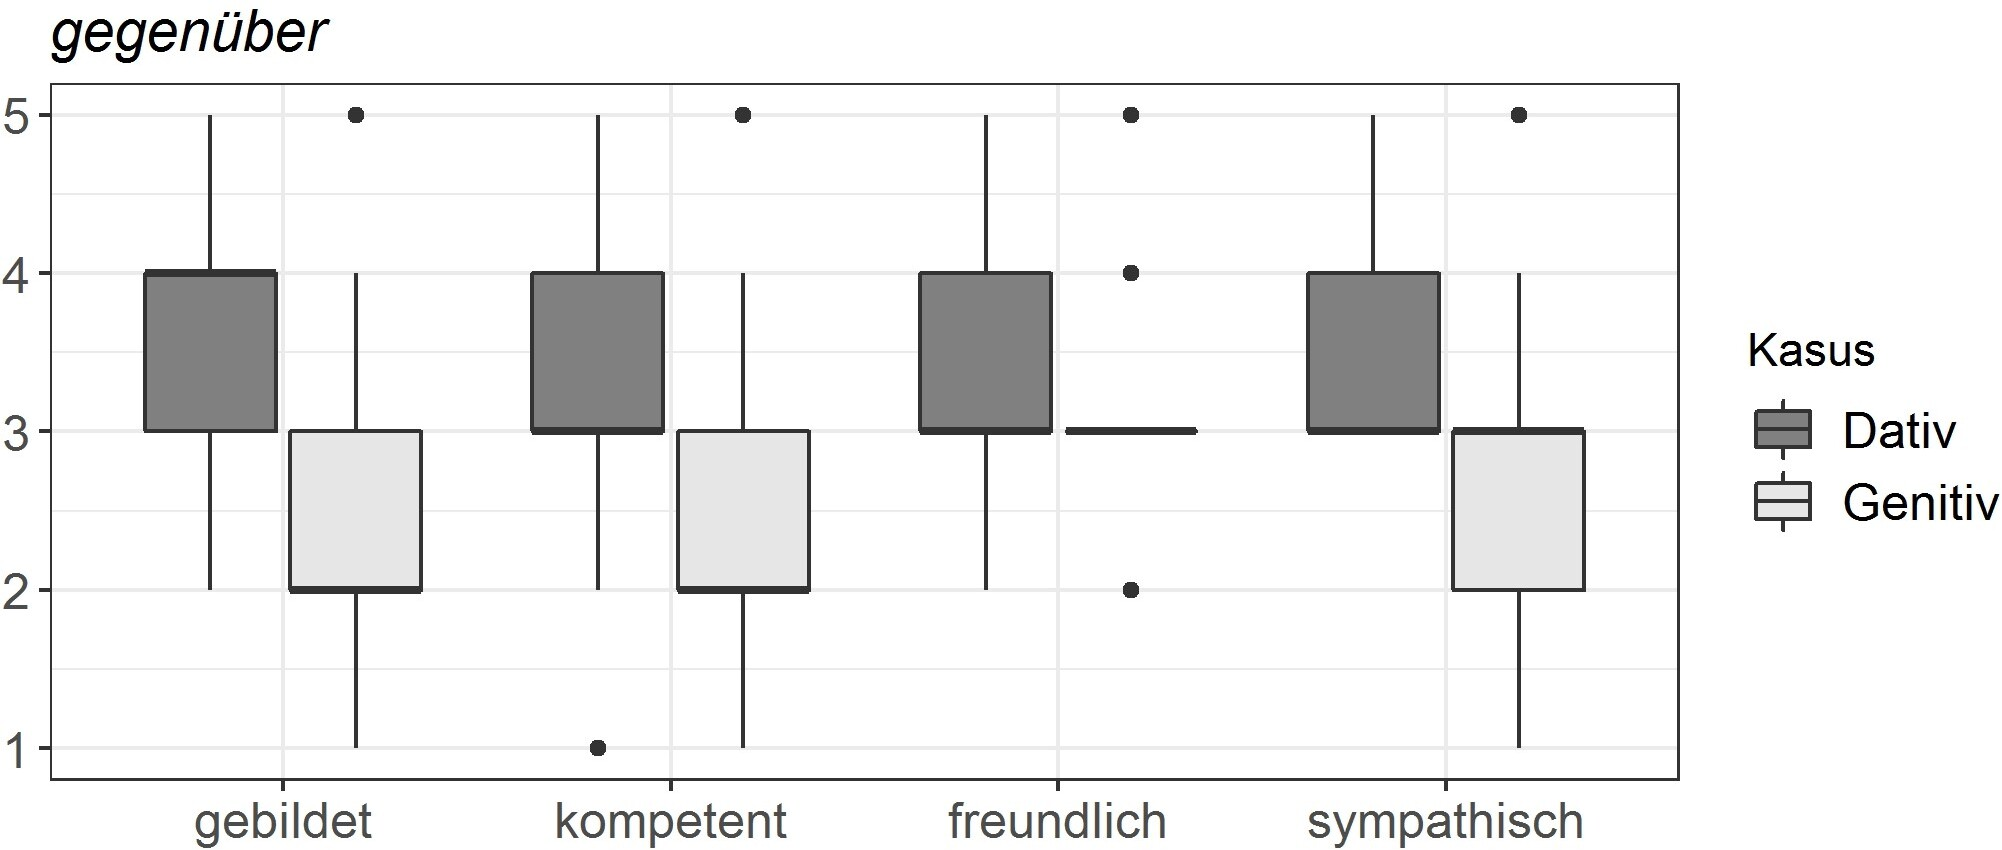
\includegraphics[width=\textwidth]{sdsgegenueberBoxplots.jpg}
\caption{Bewertung der Rektionsvarianten von \gegenueber}
\label{pic:sdsGegenueber}
\end{figure}

%In den Statuskategorien Bildung und Kompetenz scheint \gegenueber{} mit der Genitivrektion für die Befragten schwer einschätzbar zu sein: Die relativ  hohen Standardabweichungen von über 1,0 deuten hier darauf hin, dass die Einschätzungen recht unterschiedlich ausfallen. 
Für die Kategorien Freundlichkeit und Sympathie liegen die Mediane für alle Varianten bei 3. 
Auch hier werden bei den Dativvarianten aber häufiger Werte über 3 vergeben als bei den Genitivvarianten. 
Eine hohe Einigkeit herrscht offenbar darüber, dass \gegenueber{} mit dem Genitiv durchschnittlich freundlich klingt, hier beträgt der Interquartilsabstand 0.  
Bei der Bewertung der Sympathie von \gegenueber{} plus Dativ fällt zudem auf, dass die beiden niedrigsten Werte, 1 und 2, kein einziges Mal vergeben wurden. 
Die Dativrektion bei \gegenueber{} wird also von niemandem als unsympathisch empfunden.
Dies überrascht insofern wenig, als die Präposition noch kaum in ihrer Rektion schwankt und der Dativ der deutlich frequentere Kasus ist. %Änderung Anfang
Die Genitivrektion hingegen wird von einigen Befragten als wenig sympathisch beurteilt, sodass \gegenueber{} die einzige Präposition ist, bei der diese Rektionsvariante niedrige Werte in den Status- und Wärmekategorien erhält. %Änderung Ende

Insgesamt lässt sich bei allen Präpositionen erkennen, dass der Rektionskasus die Einschätzung der Freundlichkeit und Sympathie einer Person kaum beeinflusst.
Lediglich bei \dank{} unterscheiden sich die Mediane für Dativ und Genitiv bei diesen beiden Kategorien.  
Die folgende Aussage eines Befragten im freien Kommentar am Ende des Fragebogens bestätigt, dass die Kategorien Freundlichkeit und Sympathie nicht in das Bedeutungspotenzial der Rektionsvarianten fallen: 
\begin{exe}
\ex \object{Die Frage, ob eine Formulierung sympathisch ist oder nicht, finde ich schwierig, da der Tonfall und die Mimik bzw. Gestik hauptsächlich ausmacht, ob etwas sympathisch ist.} (Sozialversicherungsfachangestellter, 25)\footnote{Alle Kommentare aus dem Fragebogen werden genauso wiedergegeben, wie sie von den Befragten eingegeben wurden, also inklusive eventueller Tippfehler usw.}
\end{exe}
Anders als in vielen dialektologischen Studien zeigt sich bei den Rektionsvarianten also offenbar keine Differenzierung in dem Sinne, dass eine Variante in den Wärmekategorien besser bewertet würde, während die andere in den Statuskategorien höher eingeschätzt wird (\autoref{sec:Bewertungsgrundlage}).
Dies könnte daran liegen, dass Dialekte bzw. auch stark indexikalisch aufgeladene dialektale Varianten aufgrund ihres regionalen Bezugs ein höheres Identifikationspotenzial für Gruppen bieten als die hier abgefragten Rektionskasus.
% Änderung Anfang
Zudem könnte die hohe Bewertung beider Dimensionen für die Genitivvarianten von \wegen, \waehrend{} und \dank{} darauf hindeuten, dass diese Varianten dem Standard zugeschrieben werden und damit der Sprechergruppe, die als Referenz für alle gilt (s. dazu \autoref{sec:Bewertungsgrundlage}). %Änderung Ende

Zu der Bewertung der Rektionsvarianten auf den semantischen Differenzialen lässt sich insgesamt sagen, dass es eine starke Tendenz zur positiven Bewertung gibt. 
Dies zeigt sich etwa darin, dass die niedrigste Option auf der Bewertungsskala bei vielen Items von niemandem ausgewählt wurde. 
Der höchste Wert hingegen wurde bei allen Items vergeben -- außer im bereits angesprochenen Fall der Bewertung der Bildung bei \waehrend{} plus Dativ. 
Diese Tendenz zur positiven Bewertung kann als ein Effekt der sozialen Erwünschtheit verstanden werden (\autoref{sec:Methodologie}): 
Offenbar haben die Befragten Hemmungen, Personen aufgrund ihres Sprachgebrauchs negativ zu bewerten.
Darauf deutet auch diese Aussage eines Befragten im Kommentar am Ende des Fragebogens hin:
% \newpage 
\begin{exe}
\ex \object{Intelligenz/Kompetenz anhand von grammatikalischer Sicherheit einzuschätzen ist vielleicht noch machbar, aber ich halte es für schwierig, soziale Aspekte danach einzuschätzen, auch nicht so kluge Menschen können super lieb sein} (Student Ingenieurwissenschaften, 23)
\label{Bsp:Kommentarsds2}
\end{exe}
Die Äußerung präsupponiert, dass die Verwendung der Rektionsvarianten von der sprachlichen Sicherheit der SprachbenutzerInnen abhängt. 
Über diese Assoziation mit sprachlicher Sicherheit kann eine Variante auf einer höheren indexikalischen Ordnung geradezu ikonisch mit Eigenschaften wie Kompetenz oder Bildung verknüpft sein. 
Dies wird in einer weiteren Präsupposition der Äußerung in \autoref{Bsp:Kommentarsds2} ersichtlich, nämlich dass die Verwendung der Dativrketion darauf schließen lasse, jemand sei \object{nicht so klug}. 
Mit Eigenschaften wie Freundlichkeit oder Sympathie hingegen wird sprachliche Unsicherheit und damit auch die Dativrektion weniger stark in Verbindung gebracht. 
%Spielt hierfür vielleicht auch eine Rolle, dass nur ein Merkmal bewertet wird und nicht ein ganzes Register?

Der Kommentar in \autoref{Bsp:Kommentarsds2} zeigt bereits, dass es für eine umfassende Analyse der Indexikalität der Rektionskasus nicht ausreichend ist, Skalenwerte zu betrachten. 
Offene Fragen zu freien Assoziationen können noch sehr viel detailliertere Einblicke in die metapragmatische Bewertung der Varianten geben. 
Im folgenden Abschnitt wird die Auswertung solcher freien Assoziationen aus dem Fragebogen erläutert. 
\subsection{Überblick über die Assoziationskategorien}
\label{sec:ErgAssKat}
Wie oben bereits beschrieben, wurde je ca. 100 Befragten eine der vier Sekundärpräpositionen (\wegen, \waehrend, \dank{} oder \gegenueber) mit beiden Rektionsvarianten präsentiert (s. \autoref{table:Ass}). 
Zu jeder der beiden Rektionsvarianten wurden die Befragten nach freien Assoziationen gefragt, die sie als beliebig lange Antwort in ein Textfeld eintragen konnten. 
Aus diesem Design ergibt sich, dass insgesamt knapp unter 800 Antworten erhoben wurden (je zwei pro UntersuchungsteilnehmerIn). 
Diese wurden, wie in \autoref{sec:KategorisierungAss} beschrieben, inhaltsanalytisch in Kategorien gegliedert.
Dafür wurde mit der Software \citet{MAXQDA.19892018} gearbeitet. 
Das Kodierungshandbuch mit genauen Anweisungen für die Kategorisierung befindet sich im Anhang (\autoref{Anh:HandbuchAss}).
 
Da bereits die Assoziationskategorien Ergebnis einer ersten Analyse der freien Antworten sind, erfolgt hier einleitend eine Darstellung des Kategoriensystems. 
Diese gibt einen Überblick über die Bandbreite der Assoziationen, auf die in den darauffolgenden Abschnitten im Einzelnen eingegangen wird. 

Das Kategoriensystem besteht aus 16 Oberkategorien mit bis zu zwei Ebenen von Unterkategorien. 
Bspw. verfügt die Oberkategorie \glqq Personentypus\grqq{} über die Unterkategorie \glqq Bildung\grqq{} (erste Ebene), die wiederum die Unterkategorie \glqq gebildet\grqq{} aufweist (zweite Ebene). 
Um den Zusammenhang solcher Ober- und Unterkategorien anzuzeigen, wird hier folgende Notation verwendet: \glqq Personentypus > Bildung > gebildet\grqq.

In \autoref{table:KatsysAss} sind die 16 Oberkategorien sowie die erste Ebene der Unterkategorien aufgeführt. 
%Einige Oberkategorien verfügen über mehr als eine Ebene von Unterkategorien, etwa die eben genannte Oberkategorie \glqq Person\grqq{} oder die Oberkategorie \glqq Ästhetik\grqq, bei der sich bspw. die Unterkategorie \glqq ästhetisch\grqq{} noch einmal aufteilt in \glqq elegant/gehoben\grqq{} und \glqq gut/schön\grqq. 
Eventuell vorhandene weitere Unterkategorisierungen werden in den einzelnen Abschnitten zu den jeweiligen Oberkategorien beschrieben.
\autoref{table:Ass} zeigt neben den ersten beiden Kategorienebenen, wie viele Kodierungseinheiten jeder Oberkategorie zugewiesen wurden. 
Auf diese Verteilung wird später noch genauer eingegangen. 

\begin{table}
\small
\begin{tabular}{ll|r}
\multicolumn{2}{l|}{Oberkategorien und Unterkategorien} & Anzahl Kodierungen \\ \hline
\multicolumn{2}{l|}{Korrektheit} & 282 \\ %\hline
\textbf{} & - falsch &  \\ 
\textbf{} & - richtig &  \\ \hline
\multicolumn{2}{l|}{Zweifel} & 8 \\ \hline
\multicolumn{2}{l|}{Gleichgültigkeit} & 4 \\ \hline\multicolumn{2}{l|}{Herleitung} & 9 \\ \hline
\multicolumn{2}{l|}{Bedeutung und Verständlichkeit} & 10 \\ \hline
\multicolumn{2}{l|}{eigener Sprachgebrauch} & 23 \\ %\hline
\textbf{} & - entspricht eigenem Gebrauch nicht &  \\ 
\textbf{} & - entspricht eigenem Gebrauch &  \\ \hline
\multicolumn{2}{l|}{Sprachwandel} & 31 \\ %\hline
\textbf{} & - natürlicher Wandel &  \\ 
\textbf{} & - Sprachverfall &  \\ \hline
\multicolumn{2}{l|}{Formalität} & 89 \\ %\hline
\textbf{} & - informell &  \\ 
\textbf{} & - formell &  \\ \hline
\multicolumn{2}{l|}{Medium} & 45 \\ %\hline
\textbf{} & - schriftlich &  \\ 
\textbf{} & - mündlich &  \\ \hline
\multicolumn{2}{l|}{Varietät} & 76 \\ %\hline
\textbf{} & - Standard &  \\ 
\textbf{} & - Regionalsprache/Dialekt &  \\ 
\textbf{} & - Umgangs-/Alltagssprache &  \\ \hline
\multicolumn{2}{l|}{Ästhetik} & 195 \\ %\hline
\textbf{} & - auffällig/ungewohnt &  \\ 
\textbf{} & - unauffällig/normal &  \\ 
\textbf{} & - nicht ästhetisch &  \\ 
\textbf{} & - ästhetisch &  \\ 
\textbf{} & - simpel &  \\ \hline
\multicolumn{2}{l|}{Personentypus} & 191 \\ %\hline
\textbf{} & - Vertrautheit &  \\ 
\textbf{} & - Charakter &  \\ 
\textbf{} & - soziale Gruppe &  \\ 
\textbf{} & - Bildung &  \\ 
\textbf{} & - Sprachkompetenz &  \\ \hline
\multicolumn{2}{l|}{Stellung} & 7 \\ \hline
\multicolumn{2}{l|}{nicht relevant} & 27 \\ \hline
\multicolumn{2}{l|}{keine Assoziation} & 60 \\ \hline
\multicolumn{2}{l|}{nicht entscheidbar} & 23 \\ 
\end{tabular}
\caption{Oberkategorien und erste Ebene der Unterkategorien für die Inhaltsanalyse der freien Assoziationen}
\label{table:KatsysAss}
%\end{small}
\end{table}
%\begin{figure}[htbp]
%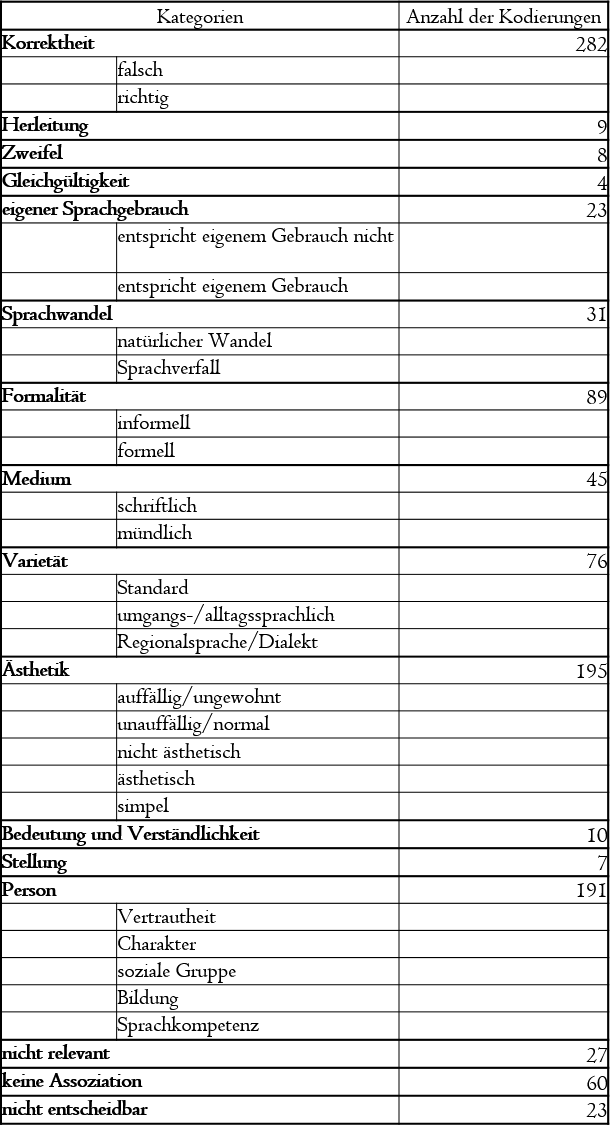
\includegraphics[scale=1]{KategoriensystemAsssw.png}
%\caption{Oberkategorien und erste Ebene der Unterkategorien für die Inhaltsanalyse der freien Assoziationen}
%\label{pic:KatsysAss}
%\end{figure}  Als Kodierungseinheit diente jeweils eine komplette Äußerung, also eine Antwort zu einer Variante.
Ein wichtiges Prinzip der Kodierung ist, dass eine Kodierungseinheit mehreren Kategorien zugeordnet werden konnte. 
Durch diese Möglichkeit der Mehrfachkodierung kommt es zu einer Gesamtzahl von 1080 Kodierungen. 
Die folgende Antwort zu \dank{} mit der Dativrektion bspw. wurde mit \glqq Formalität > informell\grqq, \glqq Medium > mündlich\grqq{} und \glqq Personentypus > Vertrautheit/Nähe\grqq{} kodiert: 
\begin{exe}
\ex \object{informelle Unterhaltung, mit vertrauten Personen, z. B. Familie, enge Freunde, befreundete Arbeitskollegen in informeller Situation}\footnote{Da die Metadaten für die Erläuterung der Kategorien nicht relevant sind, werden sie bei den in diesem Abschnitt zitierten Kommentaren nicht aufgeführt.}
\end{exe}
Wenn in einer Antwort allerdings mehrfach auf die gleiche Kategorie Bezug genommen wird, so findet sich die Antwort dennoch nur einmal in dieser Kategorie. 
Bspw. verweist die Aussage \object{locker, informell} sowohl mit \object{locker} als auch mit \object{informell} auf die Informalität von \dank{} mit dem Dativ. 
Dennoch wird die Antwort nur einmal als \glqq Formalität > informell\grqq{} kategorisiert.

Recht zahlreich finden sich Antworten, die auf die sprachliche Richtigkeit der präsentierten Variante abzielen. 
Insgesamt 282 Antworten wurden in der Oberkategorie \glqq Korrektheit\grqq{} kodiert, die damit die frequenteste Kategorie ist. 
Sie weist lediglich zwei Unterkategorien auf, nämlich \glqq richtig\grqq{} und \glqq falsch\grqq. 
Hier finden sich etwa Antworten wie \object{der Genitiv ist richtig}. 

Die Oberkategorie \glqq Zweifel\grqq{} beinhaltet Antworten, die sprachliche Zweifel ausdrücken, wie etwa diese Äußerung, die sich auf \gegenueber{} bezieht: 
\begin{exe}
\ex \object{Je öfter ich es lese, desto weniger weiß ich ob es richtig ist -- spontan bin ich unschlüssig. Ich hätte weder 1 noch 2 formuliert}. 
\end{exe}
Wenige Befragte äußern, dass sie beide Varianten gleichermaßen akzeptieren. 
Antworten wie die folgende zu \dank{} finden sich in der hierfür angelegten Kategorie \glqq Gleichgültigkeit\grqq.
\begin{exe}
\ex \object{bei dank dem/des ist mir das egal}
\end{exe}
Diese Oberkategorie weist keine Unterkategorien auf.

In den Assoziationen der Oberkategorie \glqq Herleitung\grqq{} versuchen Befragte, sprachlich zu begründen, inwiefern eine Form korrekt ist, wie etwa in folgender Antwort: 
\begin{exe}
\ex \object{Es heißt weswegen? nicht wemwegen?}
\end{exe}

In die Kategorie \glqq Bedeutung und Verständlichkeit\grqq{} fallen Antworten, die etwa darauf hinweisen, dass ein Beispiel gut oder schlecht verständlich ist oder eine bestimmte Lesart im Vordergrund steht. 
So etwa diese Aussage zu \gegenueber{} mit dem Dativ: 
\begin{exe}
\ex \object{Ich verstehe die Aussage sofort, mir fällt nichts besonderes dazu ein.}
\end{exe}
Die Kategorie \glqq Bedeutung und Verständlichkeit\grqq{} weist keine Unterkategorien auf, wie in \autoref{table:KatsysAss} zu erkennen ist.
 
%\autoref{sec:ErgAssKorrektheit} geht insbesondere auf die Assoziationen mit Korrektheit ein, da diese besonders zahlreich sind, berücksichtigt aber auch die Kategorien \glqq Herleitung\grqq, \glqq Zweifel\grqq{} und \glqq Gleichgültigkeit\grqq.
Unter der Oberkategorie \glqq eigener Sprachgebrauch\grqq{} wurden Antworten kodiert, die eine Variante mit dem eigenen Sprachgebrauch in Verbindung bringen, indem sie entweder aussagen, dass eine Variante der eigenen Verwendung entspricht oder dass eine Variante der eigenen Verwendung nicht entspricht. 
So etwa diese Antwort zu \dank{} mit der Genitivrektion: 
\begin{exe}
\ex \object{Diese Variante würde ich verwenden }
\end{exe}
In die Oberkategorie \glqq Sprachwandel\grqq{} fallen auf der einen Seite Assoziationen, die auf den natürlichen Wandel der Sprache Bezug nehmen, auf der anderen Seite solche, die eine negative Einstellung gegenüber dem Sprachwandel erkennen lassen. 
Letztere Kategorie beinhaltet vor allem die häufig getätigte Aussage \object{der Dativ ist dem Genitiv sein Tod} (vgl. \autoref{sec:IndexikalitaetRektionskasushistorisch}).

Den Oberkategorien \glqq Formalität\grqq, \glqq Medium\grqq{} und \glqq Varietät\grqq{} ist gemein, dass sie sich alle mit der Angemessenheit der Variante in bestimmten Kontexten oder der Evozierung dieser Kontexte durch die Varianten beschäftigen. 
Die Assoziationen zur Formalität lassen sich dabei in Zuschreibungen zu einem informellen Register und Zuschreibung zu einem formellen Register unterteilen. 
Darunter fallen bspw. Aussagen, die Varianten als \object{locker} oder \object{förmlich} bezeichnen. 
In die Oberkategorie \glqq Medium\grqq{} fallen Antworten, die eine Variante mit phonischer oder graphischer Realisierung in Verbindung bringen. Ein Beispiel ist diese Äußerung zu \dank{} mit der Dativrektion, die zusätzlich der Kategorie \glqq eigner Sprachgebrauch > entspricht eigenem Gebrauch\grqq{} zugeordnet wurde: 
\begin{exe}
\ex \object{Würde ich im mündlichen Sprachgebrauch verwenden}
\end{exe}
Unter \glqq Varietät\grqq{} finden sich Zuschreibungen zur Standardsprache und Beschreibungen der Variante als umgangs- oder alltagssprachlich sowie Assoziationen mit dem Sprachgebrauch einer bestimmten Region oder mit dialektalem Sprachgebrauch allgemein, wie im folgenden Beispiel:
\begin{exe}
\ex \object{Es hört sich sprachlich falsch an, kann aber auch aus einem Dialekt stammen, den ich nicht kenne.}
\end{exe}
Knapp ein Viertel der Antworten bezieht sich auf ästhetische Dimensionen einer Variante, wie etwa die folgenden: 
\begin{exe}
\ex \object{Klingt holprig} \label{Bsp:holperig}
\ex \object{Klingt komisch} \label{Bsp:komisch}
\end{exe}
Diese finden sich unter der Oberkategorie \glqq Ästhetik\grqq. 
Zum einen fallen hierunter Aussagen, die eine Variante entweder als unschön bezeichnen, wie in \autoref{Bsp:holperig}, oder aber als schön (\glqq nicht ästhetisch\grqq{} bzw. \glqq ästhetisch\grqq), zum anderen Aussagen über die Auffälligkeit oder Unauffälligkeit der Varianten, wie \autoref{Bsp:komisch} (\glqq auffällig/ungewohnt\grqq{} bzw. \glqq unauffällig/normal\grqq). 
Daneben finden sich unter der Oberkategorie \glqq Ästhetik\grqq{} außerdem einige wenige Antworten, die eine Variante als \glqq simpel\grqq{} beschreiben, z.\,B.:
\begin{exe}
\ex \object{Einfachere Sprachform} 
%(Pflegedienstleiterin, 37, zu \dank{} mit dem Dativ)
\end{exe}

In 191 Antworten finden sich Assoziationen, die mit der Produzentin oder dem Empfänger einer Variante zusammenhängen, sich also auf Eigenschaften von Personen beziehen, wie etwa das folgende Beispiel zu \dank{} mit dem Genitiv: 
\begin{exe}
\ex \object{Arroganz, Selbstgefälligkeit, gebildet} \label{Bsp:Arroganz}
\end{exe}
Unter personenbezogene Assoziationen fallen zunächst Zuschreibungen einer Variante zu bestimmten Charaktereigenschaften sowie Zuschreibungen zu sozialen Gruppen, wie etwa AkademikerInnen.
Eine eigene Unterkategorie bilden dabei Assoziationen mit niedriger oder hoher Bildung, da diese besonders zahlreich sind (\autoref{sec:ErgAssPersonen}). 
In \autoref{Bsp:Arroganz} etwa wird sowohl auf den Charakter der sich äußernden Person Bezug genommen als auch auf deren Bildung, weshalb diese Äußerung in beiden Unterkategorien kodiert ist. 
Daneben finden sich Antworten, die sich auf die Vertrautheit der InteraktionspartnerInnen beziehen. 
Außerdem nehmen einige Kommentare Bezug auf die Sprachkompetenz von Personen, die mit der Verwendung einer präsentierten Variante assoziiert werden. 

In eine weitere Kategorie fallen Assoziationen, die sich nicht auf die Rektion, sondern auf die Stellung der Präposition beziehen. 
Diese finden sich ausschließlich zur Präposition \gegenueber, bei der einige Befragte die Poststellung präferiert hätten.
Auch die Kategorie \glqq Stellung\grqq{} kommt ohne eine weitere Untergliederung aus. 

In der Kategorie \glqq nicht relevant\grqq{} wurden Antworten gesammelt, die lediglich Assoziationen enthalten, die erkennbar nicht mit der Rektion der Varianten zusammenhängen und sich meist auf den Inhalt der Beispielsätze beziehen. 
Etwa wenn ein Befragter zum Beispiel \object{Sie hat es gegenüber dem Lehrer nicht erwähnt} schreibt: 
\begin{exe}
\ex \object{Sie hat dem Lehrer etwas verschwiegen}
\end{exe}
Wenn in einer Antwort keine Assoziationen erkennbar sind, wurde die Kategorie \glqq keine Assoziation\grqq{} vergeben. 
Hierunter fallen bspw. Antworten, in denen Befragte lediglich einen Strich eingetragen oder etwas wie \object{nichts} geschrieben haben. 
Bei einigen Antworten schließlich war auch nach der gemeinsamen Durchsicht durch die drei Kodiererinnen nicht entscheidbar, in welcher Kategorie sie zu kodieren wären. 
Diese insgesamt 23 Antworten wurden als \glqq nicht entscheidbar\grqq{} gewertet. 
Dazu gehören etwa die folgenden:
\begin{exe}
\ex \object{Wer oder was, wessen, wem, wen oder was???}
\ex \object{?}
\end{exe} 
Die drei Oberkategorien, \glqq nicht relevant\grqq, \glqq keine Assoziation\grqq{} und \glqq nicht entscheidbar\grqq, sind von dem oben beschriebenem Prinzip der Mehrfachkodierung ausgeschlossen. 
Das heißt, diese Kategorien wurden nur dann vergeben, wenn eine Kodierungseinheit keine weiteren Assoziationen enthielt.
Die Antwort \object{gar keine, würde mir nicht auffallen, da richtig} bspw. wurde nicht in \glqq keine Assoziation\grqq{} kodiert, da entgegen der ersten Aussage in der Antwort Assoziationen zur Ästhetik (\glqq unauffällig/normal\grqq) und zur Korrektheit (\glqq richtig\grqq) geäußert werden.  
Dieses Vorgehen ermöglicht es, Äußerungen, die für die weitere Analyse nicht herangezogen werden können, da sie keine (relevanten) oder lediglich unklare Assoziationen enthalten, leicht zu identifizieren. 

In \autoref{pic:OKatAss2} ist zusammenfassend dargestellt, wie sich die insgesamt 1080 Kodierungen auf die hier beschriebenen 16 Oberkategorien verteilen. 
Die Kategorien sind entsprechend der Anzahl der ihnen zugeordneten Assoziationen geordnet, sodass ersichtlich wird, welche Aspekte für die Befragten besonders relevant sind.
\begin{figure}
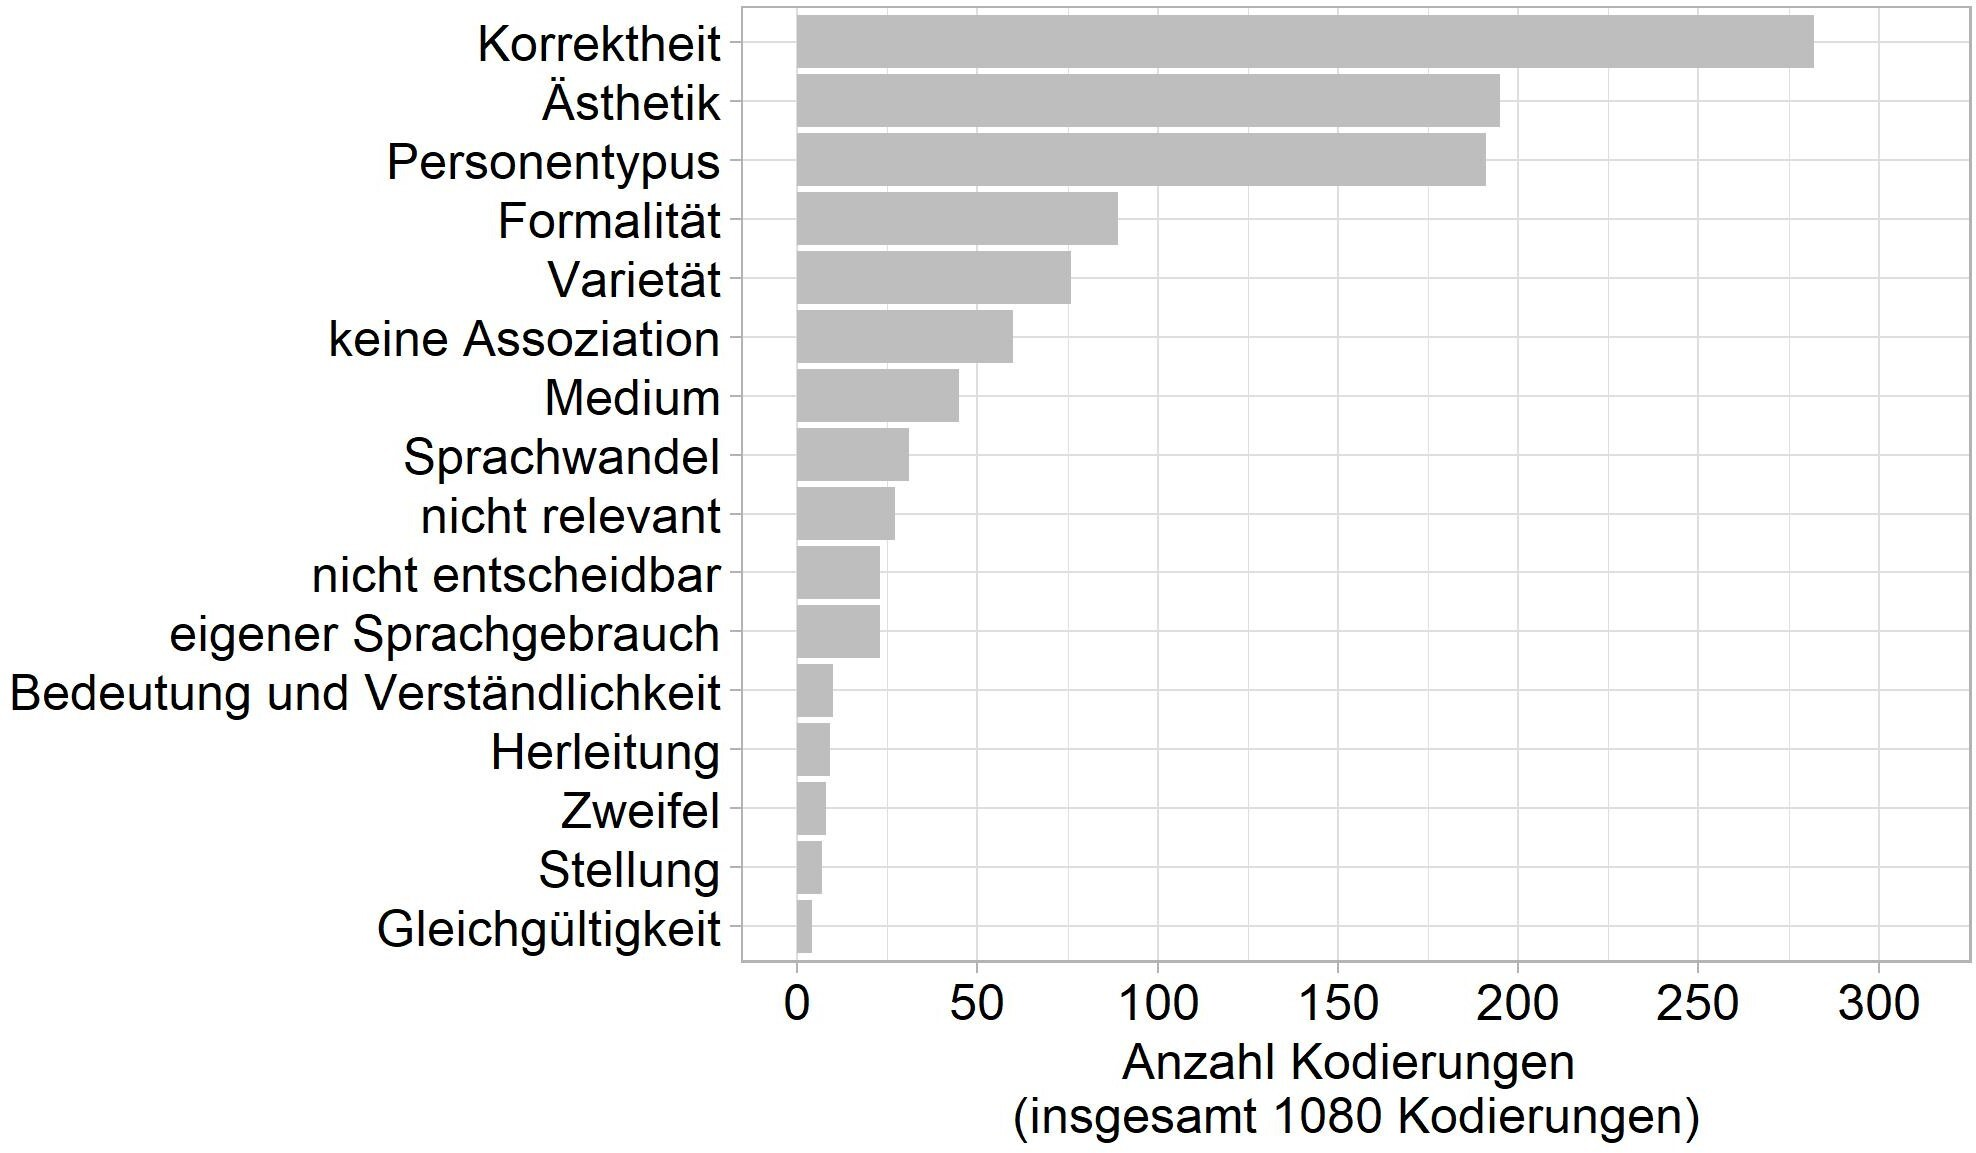
\includegraphics[width=\textwidth]{OKatAss.jpg}
\caption{Anzahl der Kodierungen in den 16 Oberkategorien}
\label{pic:OKatAss2}
\end{figure}
Demnach wird in den Antworten insbesondere auf die Korrektheit der Varianten sehr häufig verwiesen: Diese Kategorie macht ca. ein Viertel aller Kodierungen aus. 
Assoziationen mit ästhetischen Eigenschaften sowie mit Personentypen spielen ebenfalls eine wichtige Rolle. 
Auch Assoziationen mit Formalität, Varietät oder Medium sind recht zahlreich: 
89 Assoziationen betreffen die Formalität einer Variante, 45 das Medium und 76 einen varietätslinguistischen Aspekt. 
Die Oberkategorie \glqq Sprachwandel\grqq{} ist mit 31 Kodierungen ebenfalls erwähnenswert. 
Auf diese in den Assoziationen stark vertretenen Oberkategorien wird in den folgenden Abschnitten %Änderung Anfang
in der Reihenfolge ihrer Häufigkeit %Änderung Ende 
detaillierter eingegangen. 

Auch der Fall, dass keine Assoziation geäußert wurde, ist relativ häufig:
Insgesamt 60 Antworten enthalten keine Assoziationen. 
Berücksichtigt man zusätzlich Antworten der Kategorie \glqq nicht relevant\grqq{}, so ergibt dies 87 Antworten, in denen sich keinerlei Assoziation zu einem der Rektionskasus ausmachen lässt. 
Diese Beobachtung unterstreicht einen Vorteil der Erhebung freier Assoziationen gegenüber der Verwendung semantischer Differenziale: 
Während Befragte im Falle der semantischen Differenziale gezwungen sind, ein Kreuz innerhalb bereits vorgegebener Kategorien zu setzen, gibt die Frage nach freien Assoziationen den Blick frei auf Fälle, in denen Befragte mit einer Variante keine soziale Bedeutung verbinden.  

Im Anschluss an die Kategorisierung der Assoziationen wurden in MAXQDA zusätzlich die Metadaten Altersgruppe und Gender kodiert, um leichter auf diese Informationen über die Befragten zugreifen zu können. 
Jede Kodierungseinheit, also jede Antwort, verfügt daher mindestens über drei Kodierungen: Altersgruppe, Gender und mindestens eine inhaltliche Kategorie. 
\autoref{pic:ScreenshotMAXQDA} zeigt zur Veranschaulichung ein Beispiel in einem Screenshot aus MAXQDA. 
Links neben der Tabelle mit den Befragungsdaten erscheinen die vergebenen Kategorien. 
Neben der Kodierung in \glqq Korrektheit > richtig\grqq{} sind zusätzlich die Kodierungen der Metadaten zu sehen: \glqq Gender > männlich\grqq{} und \glqq Altersgruppe > 26--35\grqq.
%Falls das bunt bleibt, kurz auf die Farben eingehen! 

\begin{figure}
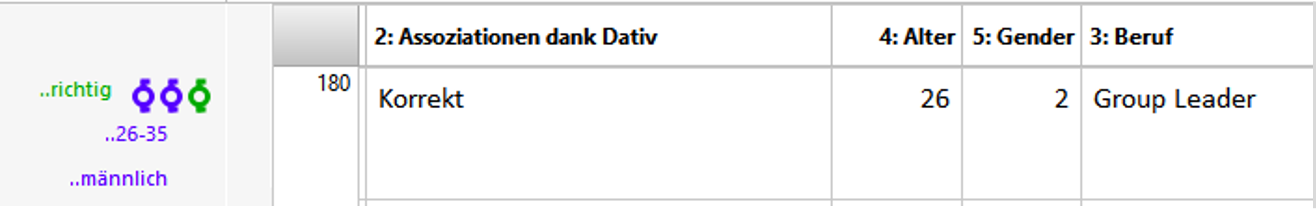
\includegraphics[width=\textwidth]{ScreenshotMAXQDAneu.png}
\caption{Screenshot aus MAXQDA: Darstellung der Kodierungen}
\label{pic:ScreenshotMAXQDA}
\end{figure}
\subsection{Assoziationen mit Korrektheit}
\label{sec:ErgAssKorrektheit}
% Korrektheit / Standardsprachideologie
Die häufigste Assoziation der Befragten ist die Zuordnung der präsentierten Variante zu den Kategorien \glqq richtig\grqq{} oder \glqq falsch\grqq. 
282 Antworten enthalten eine Assoziation zu dieser Kategorie. 
In der hohen Frequenz dieser Assoziation zeigt sich bereits die Relevanz der Standardsprachideologie und der damit verbundenen Annahme, es gebe stets nur eine korrekte Variante (\autoref{sec:Einheitlichkeit}). 
Offenbar führt die Konfrontation mit zwei Rektionsvarianten bei sehr vielen Befragten zu dem Bedürfnis, Richtig von Falsch zu unterscheiden. 
Welche Varianten sie dabei als richtig bezeichnen und welche als falsch, zeigt \autoref{pic:AssKorrektheit}. 

\begin{figure}
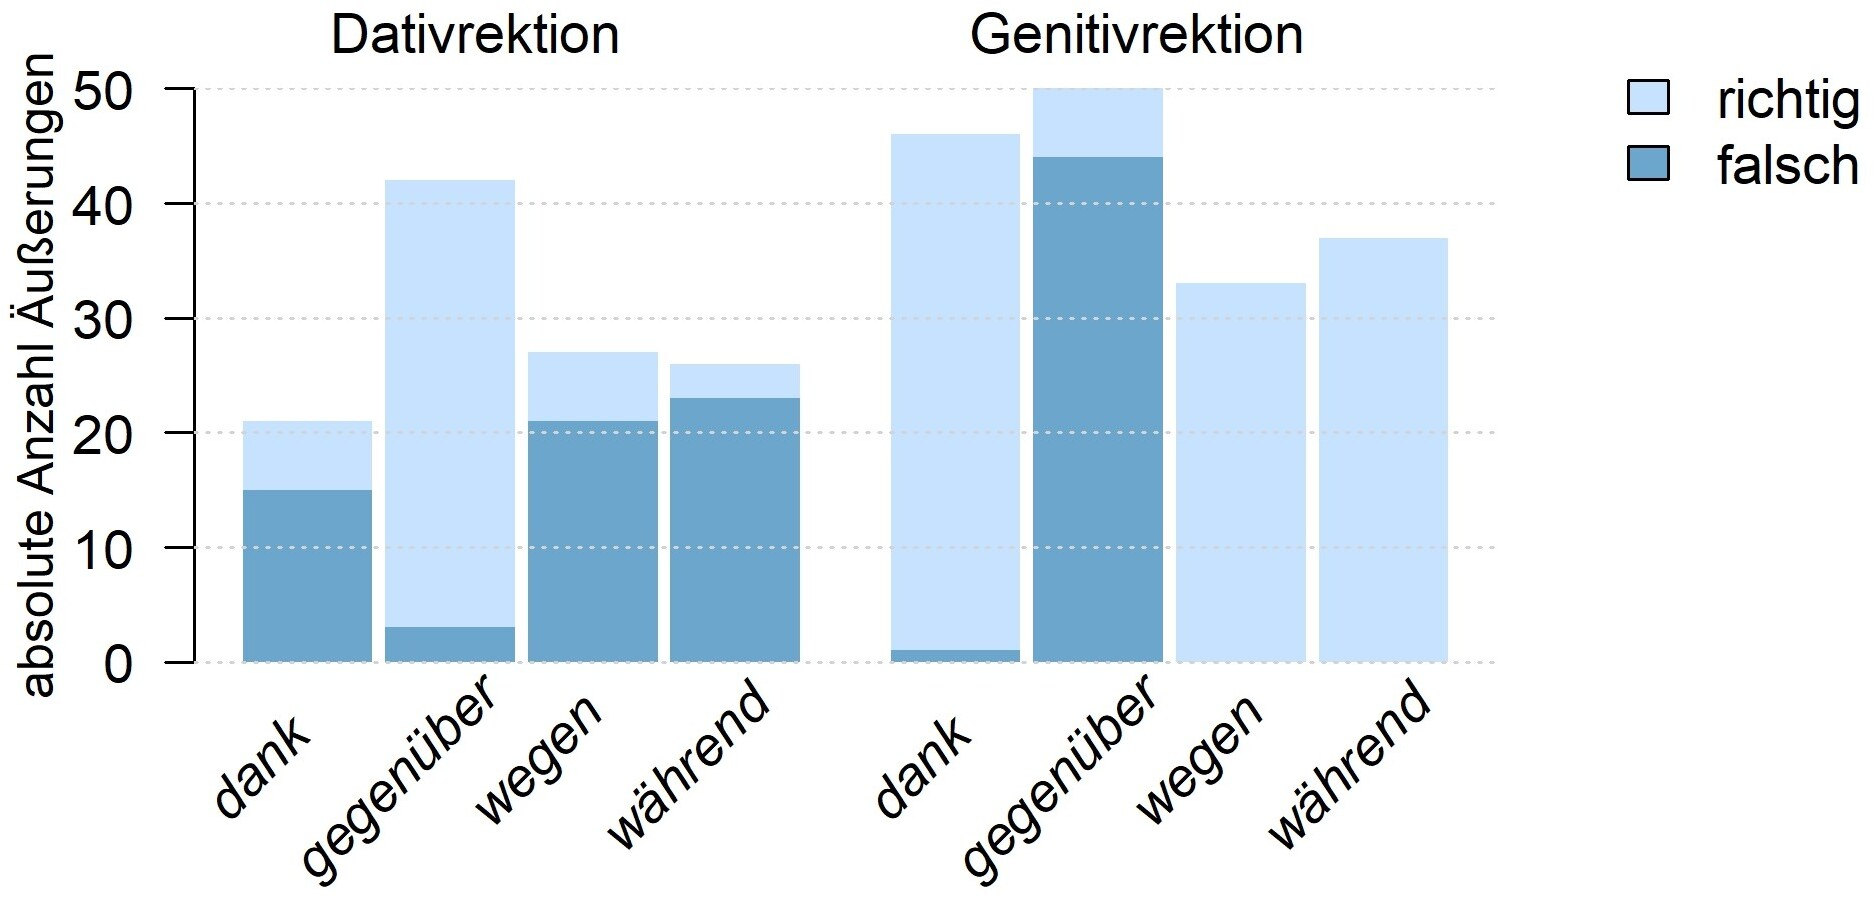
\includegraphics[width=\textwidth]{AssKorrektheit.jpg}
\caption{Verteilung der Assoziationen der Oberkategorie \glqq Korrektheit\grqq}
\label{pic:AssKorrektheit}
\end{figure}
Sowohl bei den ursprünglichen Genitivpräpositionen \wegen{} und \waehrend{} als auch bei der ursprünglichen Dativpräposition \dank{} überwiegen die Antworten, in denen die Dativrektion als falsch bezeichnet wird. 
Insgesamt finden sich 59 Äußerungen, die die Dativrektion als inkorrekt ansehen (für die genauen Zahlen s. auch \autoref{table:richtigfalschAnh} im Anhang). 
Die Genitivrektion wird bei \wegen, \waehrend{} und \dank{} beinahe ausschließlich als richtig angesehen: 
In insgesamt 116 Einstellungsäußerungen zu einer dieser drei Präpositionen mit dem Genitiv wird die Variante 115-mal als richtig bezeichnet.
Lediglich einmal bei \dank{} wird der Genitiv als falsch bezeichnet, allerdings mit dem Hinweis, dass \dank{} plus Genitiv zunächst richtig erscheine: 
\begin{exe}
\ex \object{Klingt richtig und vor allem bemüht richtig, ist aber falsch. Eselsbrücke: dank dir und nicht dank deiner} (Hotelrezeptionistin, 30, zu \dank{} mit dem Genitiv)\label{Bsp:bemueht}
\end{exe}
Die Aussage, der Genitiv klinge hier zwar korrekt, sei es in diesem Fall aber nicht, zeigt, wie stark der Genitiv mit Korrektheit in Verbindung gebracht wird.
Wird die Dativrektion als korrekte Variante bezeichnet, erscheint dies wie eine Ausnahme. 

Anders verhält es sich bei der Präposition \gegenueber{}: 
Hier wird die Genitivrektion, die noch sehr infrequent ist, von vielen als falsch empfunden.
Nur sechs Antworten bezeichnen die Genitivrektion bei \gegenueber{} als richtig. 
Interessant ist, dass es zu \gegenueber{} im Vergleich mit den anderen Präpositionen besonders viele Einstellungsäußerungen gibt, die auf die Korrektheit der Varianten Bezug nehmen. 
Dies kann ein erster Hinweis darauf sein, dass die Variation bei dieser Präposition (noch) keine starken anderen Assoziationen hervorruft, also kaum indexikalisch aufgeladen ist. 
%Darauf wird in \autoref{sec:Felder} näher eingegangen.

Bei einer näheren Betrachtung der Antworten in der Kategorie \glqq Korrektheit\grqq{} fällt auf, dass die Korrektheit unterschiedlich legitimiert wird: 
Während einige Antworten ein persönliches Korrektheitsempfinden anführen (\autoref{Bsp:irgendwiefalsch} und \autoref{Bsp:erscheintmirnichtrichtig}), werden die präsentierten Varianten in anderen Antworten kategorisch als falsch oder richtig dargestellt (\autoref{Bsp:falscherArtikel} und \autoref{Bsp:gehtdoch}). 
\begin{exe}
\ex \object{Klingt irgendwie falsch} (Postbeamtin, 53, zu \dank{} mit dem Dativ) \label{Bsp:irgendwiefalsch}
\ex \object{Erscheint mir nicht richtig, da der falsche Artikel verwendet wird.} (Biologiedoktorandin, 29, zu \dank{} mit dem Dativ) \label{Bsp:erscheintmirnichtrichtig}
\ex \object{Falscher Artikel} (Biologiestudent, 24, zu \dank{} mit dem Dativ) \label{Bsp:falscherArtikel}
\ex \object{Geht doch, richtig!} (Abteilungsleiterin, 51, zu \dank{} mit dem Genitiv) \label{Bsp:gehtdoch}
\end{exe}
Außerdem machen Antworten, in denen eine Variante als falsch bezeichnet wird, teilweise eine Einschränkung, indem sie einräumen, eine Variante sei zwar falsch, aber dennoch akzeptabel oder gebräuchlich.
So schreibt eine 19-jährige Psychologiestudentin zu \waehrend{} mit dem Dativ:
\begin{exe}
\ex \object{Falsch aber umgangssprachlich verbreitet und ok} (Psychologiestudentin, 19, zu \waehrend{} mit dem Dativ) \label{Bsp:falschumgangssprachlich}
\end{exe}
Hier zeigt sich die Annahme, dass Richtig und Falsch in der Sprache starre Kategorien sind, die unabhängig vom Sprachgebrauch feststehen. 
Als richtig scheint dabei die Variante empfunden zu werden, die als standardsprachlich registriert ist. 
Zu einem anderen Schluss kommt ein 26-jähriger Doktorand in seiner Äußerung zu \dank{} mit dem Dativ: 
\begin{exe}
\ex \object{Auch richtig, aber eher weniger im akademischen Kontext -> privat} (Geschichtsdoktorand, 26, zu \dank{} mit dem Dativ)
\end{exe}
Auch hier wird eine Unterscheidung zwischen sprachlicher Korrektheit und sprachlicher Angemessenheit getroffen. 
Jedoch wird der thematisierten Variante nicht nur eine eingeschränkte Angemessenheit, sondern auch eine eingeschränkte Korrektheit zugesprochen. 
Auf die Zusammenhänge zwischen Korrektheit und Angemessenheit wird in der Analyse der Ergebnisse des Akzeptabilitätstests (\autoref{sec:ErgAkzallg}) zurückzukommen sein. 

118 der 282 Äußerungen in der Kategorie \glqq Korrektheit\grqq{} wurden zusätzlich einer oder mehreren weiteren Kategorien zugeordnet, beziehen sich also nicht ausschließlich auf die Korrektheit der Variante, sondern daneben auf weitere Assoziationsbereiche. 
Besonders häufig (50-mal) werden Äußerungen zur Korrektheit etwa mit Assoziationen zur Ästhetik einer Variante kombiniert. 
\begin{exe}
\ex \object{klingt korrekt, eleganter bzw. flüssiger} (Wissenschaftliche Mitarbeiterin, 27, zu \dank{} mit dem Genitiv)
\end{exe} 
In diesem Beispiel wird zunächst lediglich ausgesagt, dass \dank{} mit der Genitivrektion korrekt erscheint, ohne dass die Variante mit der Dativrektion dabei als inkorrekt dargestellt wird. 
Die Komparativformen \object{eleganter} und \object{flüssiger} können aber als Vergleich mit der Dativrektion interpretiert werden, da beide Varianten im Fragebogen in direkter Opposition zueinander präsentiert werden. 
Hier wird also gewissermaßen für die Genitivvariante argumentiert, indem gesagt wird, dass diese nicht nur die Voraussetzung erfüllt, korrekt zu sein, sondern darüber hinaus ästhetischer erscheint als die Dativvariante. 

Im folgenden Beispiel wird \waehrend{} plus Dativ nicht nur als inkorrekt und unästhetisch bezeichnet, sondern außerdem mit ungebildeten SprecherInnen in Verbindung gebracht: 
\begin{exe}
\ex \object{Verkehrt, unschön, hohle Birne} (Jurastudentin, 25, zu \waehrend{} mit dem Dativ) \label{Bsp:hohleBirne}
\end{exe}
Solche Antworten, in denen Assoziationen zur Korrektheit einer Variante mit Assoziationen zu Personen kombiniert sind, finden sich in den Daten insgesamt 30-mal. 
47-mal werden Aussagen über die Korrektheit mit Aussagen zur Formalität, dem Medium oder der Varietät verbunden, wie etwa in \autoref{Bsp:falschumgangssprachlich} oben. 

Der quantitative und qualitative Blick auf die insgesamt 282 Assoziationen mit Korrektheit zeigt erstens, dass die Genitivrektion bei \wegen, \waehrend{} und \dank{} gängigerweise mit korrektem Sprachgebrauch assoziiert wird. 
Zweitens wird die Korrektheit einer Variante entweder absolut gesetzt oder aber über das eigene Sprachgefühl legitimiert. 
Drittens schließt die Einstufung einer Variante als inkorrekt nicht aus, dass die Form trotzdem als angemessen empfunden wird. 
\subsection{Assoziationen mit Ästhetik}
\label{sec:ErgAssAes}
% Ästhetik 
Ein großer Teil der Assoziationen lässt sich dem Bereich Ästhetik zuordnen (195 Antworten). 
Die Kategorie \glqq Ästhetik\grqq{} verfügt, wie oben beschrieben, über fünf Unterkategorien: \glqq unauffällig/normal\grqq, \glqq auffällig/ungewohnt\grqq, \glqq ästhetisch\grqq, \glqq nicht ästhetisch\grqq{} und \glqq simpel\grqq. 
Die Antworten, die eine Variante als \glqq ästhetisch\grqq{} oder \glqq nicht ästhetisch\grqq{} beschreiben, also Ästhetik im engeren Sinne betreffen, lassen sich wiederum mehreren Unterkategorien zuordnen, sodass das vollständige Kategoriensystem für Assoziationen zur Ästhetik aussieht, wie in \autoref{table:KatAesthetik} dargestellt.  
\begin{table}
\centering
\begin{tabular}{lll}
\lsptoprule
\multicolumn{2}{l}{Ästhetik} \\
\midrule
\multicolumn{2}{l}{- unauffällig/normal} \\
\multicolumn{2}{l}{- auffällig/ungewohnt} \\
\multicolumn{2}{l}{- ästhetisch} \\
 & - gut/schön \\ 
 & - elegant/gehoben \\
\multicolumn{2}{l}{- nicht ästhetisch} \\
 & - schlecht/unschön \\ 
 & - umständlich \\ 
 & - gestelzt/abgehoben/überkorrekt\\
 & - plump/schlampig \\ \hline
\multicolumn{2}{l}{- simpel}\\ 
\lspbottomrule
\end{tabular}
\caption{Kategorisierung der Assoziationen mit Ästhetik}
\label{table:KatAesthetik}
\end{table}

Diese Assoziationskategorien werden nun der Reihe nach besprochen.
Die Kategorie \glqq simpel\grqq{} wird dabei nicht weiter berücksichtigt, da hier lediglich drei Antworten eingeordnet wurden, von denen zwei zusätzlich in die Kategorie \glqq plump/schlampig\grqq{} fallen. 
%Wie sich die Assoziationen zu den im Fragebogen präsentierten Beispielen auf der ersten dieser Kategorienebenen verteilen, geht aus \autoref{table:AssAesthetik} hervor.
%Da es sich um freie Assoziationen handelt, sind die Zahlen teilweise sehr klein und für eine quantitative Auswertung nicht geeignet. 
%Sie sollen daher lediglich dazu dienen, besonders auffällige Verteilungen zu identifizieren, auf die ich im Folgenden näher eingehe. 
% Please add the following required packages to your document preamble:
% \usepackage[table,xcdraw]{xcolor}
% If you use beamer only pass "xcolor=table" option, i.e. \documentclass[xcolor=table]{beamer}
%\begin{table}
%\begin{tabular}{crrrrr}
%\multicolumn{1}{c}{\textit{}} & \multicolumn{1}{c}{\textbf{\begin{tabular}[c]{@{}c@{}}unauffällig/\\ normal\end{tabular}}} & \multicolumn{1}{c}{\textbf{\begin{tabular}[c]{@{}c@{}}auffällig/\\ ungewohnt\end{tabular}}} & \multicolumn{1}{c}{\textbf{ästhetisch}} & \multicolumn{1}{l}{\textbf{\begin{tabular}[c]{@{}c@{}}nicht\\ ästhetisch\end{tabular}}} & \multicolumn{1}{l}{\textbf{simpel}} \\ \hline
%\rowcolor[HTML]{C0C0C0} 
%\begin{tabular}[c]{@{}c@{}}\dank\\+ Dativ\end{tabular}          & 1	& 2	& 1	& 7	& 2                                   \\ \hline
%\rowcolor[HTML]{C0C0C0} 
%\begin{tabular}[c]{@{}c@{}}\gegenueber\\+ Dativ\end{tabular}      & 22 &	1	& 8	& 2	& 0                       \\ \hline
%\rowcolor[HTML]{C0C0C0} 
%\begin{tabular}[c]{@{}c@{}}\wegen\\+ Dativ\end{tabular}            & 6 &	3	& 0	& 9	& 0                            \\ \hline
%\rowcolor[HTML]{C0C0C0} 
%\begin{tabular}[c]{@{}c@{}}\waehrend\\+ Dativ\end{tabular}       & 3 &	6	& 1	& 15	& 1       \\ \hline
%\begin{tabular}[c]{@{}c@{}}\dank\\+ Genitiv\end{tabular}          & 1 &	1 & 9 & 6	& 0                      \\ \hline
%\begin{tabular}[c]{@{}c@{}}\gegenueber\\+ Genitiv\end{tabular}    &            0 &	20	& 1	& 18	& 0 \\ \hline
%\begin{tabular}[c]{@{}c@{}}\wegen\\+ Genitiv\end{tabular}          & 8 &	4	& 6	& 8	& 0             \\ \hline
%\begin{tabular}[c]{@{}c@{}}\waehrend\\+ Genitiv\end{tabular}      & 4 &	1	& 13	& 5	& 0          \\ 
%\end{tabular}
%\caption{Auszählung der Assoziationen mit Ästhetik}
%\label{table:AssAesthetik}
%\end{table}

\autoref{table:AssUnauffaelligAuffaellig} zeigt, wie sich die Assoziationen zu den ersten beiden Ästhetikkategorien, \glqq unauffällig/normal\grqq{} und \glqq auffällig/ungewohnt\grqq{} auf die im Fragebogen präsentierten Beispiele verteilen. 
\begin{table}
\centering
\begin{tabular}{lrr}
\multicolumn{1}{c}{\textit{}} & \multicolumn{1}{c}{\textbf{\begin{tabular}[c]{@{}c@{}}unauffällig/\\ normal\end{tabular}}} & \multicolumn{1}{c}{\textbf{\begin{tabular}[c]{@{}c@{}}auffällig/\\ ungewohnt\end{tabular}}} \\ \hline
\rowcolor[HTML]{C0C0C0} 
\dank{} + Dativ     & 1	& 2 		\\ %\hline
\rowcolor[HTML]{C0C0C0} 
\gegenueber{} + Dativ   & 22 &	1	\\ %\hline
\rowcolor[HTML]{C0C0C0} 
\wegen{} + Dativ    & 6 &	3	   \\ %\hline
\rowcolor[HTML]{C0C0C0} 
\waehrend{} + Dativ   & 3 &	6	   \\ %\hline
\dank{} + Genitiv     & 1 &	1      \\ %\hline
\gegenueber{} + Genitiv   &   0 & 20	\\ %\hline
\wegen{} + Genitiv     & 8 & 4 		\\ %\hline
\waehrend{} + Genitiv  & 4 &	1	\\ 
\end{tabular}
\caption{Auszählung der Assoziationen mit Unauffälligkeit/Auffälligkeit}
\label{table:AssUnauffaelligAuffaellig}
\end{table}

Als auffällig und ungewohnt wird hauptsächlich das Beispiel \object{sie hat es gegenüber des Lehrers nicht erwähnt} beschrieben (20-mal).
Dies erklärt sich durch die niedrige Frequenz der Genitivrektion bei \gegenueber. 
\object{Gegenüber} plus Dativ wird ebenso erwartbar häufig als unauffällig dargestellt (22-mal). 

Insgesamt betreffen von den Assoziationen aus der Kategorie \glqq Ästhetik\grqq{} recht viele die Präposition \gegenueber:
72-mal wird in Kommentaren zu den \gegenueber -Varianten auf ästhetische Eigenschaften verwiesen, so häufig wie bei keiner anderen Präposition.
Dabei handelt es sich um eher vage Assoziationen, wie Beispiele zeigen: 
\begin{exe}
\ex \object{Klingt komisch} (Geografin, 32, zu \gegenueber{} mit dem Genitiv)
\ex \object{Befremdlich} (Bürokauffrau, 28, zu \gegenueber{} mit dem Genitiv)
\ex \object{normaler Ausdruck} (Englischlehrerin, 61, zu \gegenueber{} mit dem Dativ)
\end{exe}
Offenbar erscheinen den Befragten die Rektionsvarianten von \gegenueber{} gut oder schlecht, ohne dass sie sie genauer einordnen können. 
Dies erinnert an die Beobachtungen zu den Assoziationen mit Korrektheit in \autoref{sec:ErgAssKorrektheit} und deutet erneut auf eine recht geringe Indexikalität dieser Varianten hin.

Noch häufiger als über die Auffälligkeit einer Form wird in den Kommentaren etwas darüber ausgesagt, ob sie ästhetisch oder unästhetisch erscheint. 
Die Assoziationen zur Ästhetik im engeren Sinne reichen von allgemeinen Urteilen wie \object{klingt besser} bis zu spezifischeren Zuschreibungen wie \object{umständlich} oder \object{hochgestochen}. 
\autoref{table:AssAesthetischNichtAesthetisch} zeigt die Verteilung auf die einzelnen Unterkategorien von \glqq ästhetisch\grqq{} und \glqq nicht ästhetisch\grqq.
Da es sich um freie Assoziationen handelt, sind die Zahlen teilweise sehr klein und für eine quantitative Auswertung nicht geeignet. 
Sie können aber dazu dienen, besonders auffällige Verteilungen zu identifizieren, auf die ich im Folgenden näher eingehe. 
% Please add the following required packages to your document preamble:
% \usepackage[table,xcdraw]{xcolor}
% If you use beamer only pass "xcolor=table" option, i.e. \documentclass[xcolor=table]{beamer}
\begin{table}
\centering
\begin{tabular}{lrr|rrrr}
\multicolumn{1}{c}{\textit{}} & \multicolumn{2}{c|}{ästhetisch} & \multicolumn{4}{c}{nicht ästhetisch} \\ \hline
\multicolumn{1}{c}{\textit{}} & \multicolumn{1}{c}{\begin{tabular}[c]{@{}c@{}}gut/\\ schön\end{tabular}} & \multicolumn{1}{c|}{\begin{tabular}[c|]{@{}c@{}}elegant/\\ gehoben\end{tabular}} & \multicolumn{1}{c}{\begin{tabular}[c]{@{}c@{}}schlecht/\\ unschön\end{tabular}} & \multicolumn{1}{c}{\begin{tabular}[c]{@{}c@{}}gestelzt/\\ abgehoben\end{tabular}} & \multicolumn{1}{c}{\begin{tabular}[c]{@{}c@{}}umständ-\\lich\end{tabular}} & \multicolumn{1}{c}{\begin{tabular}[c]{@{}c@{}}plump/\\ schlampig\end{tabular}}\\ \hline
\rowcolor[HTML]{C0C0C0} 
\begin{tabular}[c]{@{}c@{}}\dank\\+ Dativ\end{tabular}          & 1	& 0	& 2	& 0	& 0	& 5
                                   \\ %\hline
\rowcolor[HTML]{C0C0C0} 
\begin{tabular}[c]{@{}c@{}}\gegenueber\\+ Dativ\end{tabular}       & 8	& 0	& 2	& 0	& 0	& 0
    \\ %\hline
\rowcolor[HTML]{C0C0C0} 
\begin{tabular}[c]{@{}c@{}}\wegen\\+ Dativ\end{tabular}        & 0	& 0	& 7	& 0	& 0	& 2
     \\ %\hline
\rowcolor[HTML]{C0C0C0} 
\begin{tabular}[c]{@{}c@{}}\waehrend\\+ Dativ\end{tabular}       & 1	& 0	& 11	& 0	& 1	& 3
	 \\ %\hline
\begin{tabular}[c]{@{}c@{}}\dank\\+ Genitiv\end{tabular}          & 7	& 2	& 2	& 2	& 2	& 0
    \\ %\hline
\begin{tabular}[c]{@{}c@{}}\gegenueber\\+ Genitiv\end{tabular}    & 0	& 1	& 8	& 9	& 1	& 0
 \\ %\hline
\begin{tabular}[c]{@{}c@{}}\wegen\\+ Genitiv\end{tabular}          & 6	& 0	& 0	& 6	& 2	& 0
   \\ %\hline
\begin{tabular}[c]{@{}c@{}}\waehrend\\+ Genitiv\end{tabular}      & 10	& 3	& 0	& 5	& 0	& 0
  \\ 
\end{tabular}
\caption{Auszählung der Assoziationen mit Ästhetik im engeren Sinn}
\label{table:AssAesthetischNichtAesthetisch}
\end{table}

Schaut man auf die einzelnen Präpositionen, fällt auf, dass es lediglich bei \gegenueber{} und \waehrend{} eine klare Verteilung zwischen den Kategorien \glqq ästhetisch\grqq{} und \glqq nicht ästhetisch\grqq{} gibt: 
Bei \gegenueber{} wird die Dativrektion eher als ästhetisch empfunden, während die infrequente Genitivrektion überwiegend als nicht ästhetisch eingestuft wird. 
Bei \waehrend{} wird die Dativrektion häufig als unästhetisch bezeichnet (insgesamt 15-mal), die Genitivrektion hingegen als ästhetisch (13-mal). 
Auch bei \dank{} und \wegen{} beurteilen die Befragten die Dativrektion beinahe ausschließlich als unästhetisch. 
Weniger eindeutig ist das Bild bezüglich der Ästhetik der Genitivrektion bei \dank{} und \wegen{}:
Sie wird im den Kommentaren mal als ästhetisch, mal als unästhetisch bezeichnet. 

Insgesamt gibt es unter den Befragten eine relativ klare Tendenz dazu, die Dativvarianten als wenig ästhetisch zu beurteilen (außer bei \gegenueber), während die Meinungen bei den Genitivvarianten auseinander gehen (auch hier mit Ausnahme von \gegenueber). 
Die jeweiligen Unterkategorien von \glqq ästhetisch\grqq{} und \glqq nicht ästhetisch\grqq{} erlauben nun ein differenzierteres Bild. 
Hier sind insbesondere die Assoziationen interessant, die eine Variante nicht nur allgemein als bspw. gut oder schön bezeichnen, sondern ihr spezifischere Eigenschaften zuschreiben, wie elegant, gehoben, gestelzt, abgehoben, umständlich, plump oder schlampig.
Die positiv assoziierten Eigenschaften elegant und gehoben scheinen für den Genitiv reserviert zu sein. 
Positive Eigenschaften, die die Ästhetik betreffen und nur dem Dativ zugeschrieben werden, werden in den Assoziationen hingegen nicht genannt. 
Schaut man auf die negativen Eigenschaften, ergibt sich folgende Aufteilung: 
Wird der Genitiv als unästhetisch beurteilt, dann oftmals, weil er als gestelzt, abgehoben oder umständlich empfunden wird: 
\begin{exe}
\ex \object{Richtig, aber gestelzt} (Grundschullehrerin, 69, zu \dank{} mit dem Genitiv)
\end{exe}
Der Dativ hingegen gilt als plump oder schlampig: 
\begin{exe}
\ex \object{Hört sich eimfach und plump an} (Erzieher, 33, zu \waehrend{} mit dem Dativ)
\end{exe}

Besonders stark scheint die indexikalische Verknüpfung zwischen dem Genitiv und Gestelztheit bzw. Abgehobenheit. 
Diese Eigenschaften werden auch mit der Genitivrektion bei \gegenueber{} assoziiert: 
\begin{exe}
\ex \object{Ungewöhnlich, falsch, hochgestochen} (Sozialpädagogin, 24, zu \gegenueber{} mit dem Genitiv)
\end{exe}
Die Genitivrektion bei \gegenueber{} wird zunächst als ungewohnt und zusätzlich als falsch bezeichnet, was auf ihre geringe Frequenz zurückgeführt werden kann. 
Darüber hinaus empfindet die Befragte die Variante als \glqq hochgestochen\grqq, eine Eigenschaft, die auch den frequenten Genitivvarianten \wegen{} plus Genitiv und \waehrend{} plus Genitiv zugeschrieben wird. 

Zusammenfassend lässt sich Folgendes festhalten: 
Auffälligkeit und Unauffälligkeit sind für die Befragten insbesondere bei der Präposition \gegenueber{} relevante Bezugsgrößen, da sich hier die Rektionsvarianten in ihrer Frequenz stark unterscheiden. 
Die Dativrektion bei \dank, \wegen{} und \waehrend{} beurteilen die Befragten recht einmütig als unästhetisch: Insgesamt finden sich 31 Antworten, die diese Varianten als unästhetisch bezeichnen, und nur zwei, die sie als ästhetisch einstufen. 
Bei den Genitivvarianten von \dank, \wegen{} und \waehrend{} herrscht mehr Uneinigkeit. 
Sie werden 28-mal als ästhetisch beurteilt und 19-mal als unästhetisch. 
Der Genitiv wird als gestelzt, abgehoben und umständlich empfunden, der Dativ dagegen als plump und schlampig. 
Als elegant und gehoben gilt nur der Genitiv. 
\subsection{Assoziationen mit Personentypen}
\label{sec:ErgAssPersonen}
% Personentypen 
Eine besonders interessante Gruppe von Antworten sind die, in denen die Rektionsvarianten mit bestimmten Personentypen assoziiert werden. 
Gemessen an ihrer Anzahl haben diese Assoziationen eine große Relevanz für die Befragten: 
Insgesamt 191 Assoziationen fallen in die Kategorie \glqq Personentypus\grqq. 
Die Assoziationen betreffen die Vertrautheit der KommunikationspartnerInnen, die Bildung von Personen, denen die Variante zugeschrieben wird, ihre Sprachkompetenz, ihre soziale Gruppe und ihren Charakter. 
Das gesamte Kategoriensystem zu Assoziationen mit dem Personentypus ist in \autoref{table:KatPerson} dargestellt. 
Die ersten drei Kategorien, \glqq Vertrautheit\grqq, \glqq Bildung\grqq{} und \glqq Sprachkompetenz\grqq{} spalten sich jeweils nur in zwei Unterkategorien auf. 
Die Kommentare der Kategorien \glqq soziale Gruppe\grqq{} und \glqq Charaktereigenschaften\grqq{} verteilen sich hingegen auf zahlreiche verschiedene Unterkategorien. 

\begin{table}
\centering
\begin{tabular}{lll}
\multicolumn{2}{l}{Personentypus} \\ \hline
\multicolumn{2}{l}{- Vertrautheit} \\ %\hline
 & - Vertrautheit/Nähe \\ 
 & - Fremdheit/Distanz \\ \hline
\multicolumn{2}{l}{- Bildung} \\ %\hline
 & - hohe Bildung \\ 
 & - niedrige Bildung \\  \hline
\multicolumn{2}{l}{- Sprachkompetenz} \\ %\hline
 & - hohe Sprachkompetenz \\ 
 & - mangelnde Sprachkompetenz \\  \hline
\multicolumn{2}{l}{- soziale Gruppe} \\ %\hline
 & - AkademikerInnen/GymnasiastInnen \\
 & - beruflich Erfolgreiche \\
 & - Bourgeoisie \\
 & - ArbeiterInnen \\
 & - Unterschicht \\
 & - Technische Berufe \\ \hline
\multicolumn{2}{l}{- Charakter} \\ %\hline
 & - präzise/professionell \\ 
 & - vornehm/altmodisch \\
 & - sympathisch/mir ähnlich \\
 & - besserwisserisch \\
 & - unfreundlich \\
 & - streng/seriös \\
 & - locker/unprätentiös \\
 & - abgehoben/arrogant \\
 & - pedantisch/verkrampft \\
 & - nachlässig/schlampig \\
\end{tabular}
\caption{Kategorisierung der Assoziationen mit Personentypen}
\label{table:KatPerson}
\end{table}

Die Vertrautheit der KommunikationspartnerInnen hat weniger mit festen Personeneigenschaften als mit der Beziehung der an einer Interaktion Beteiligen zu tun. 
Damit bildet diese Kategorie ein Bindeglied zwischen Assoziationen zur Formalität und Assoziationen zu weniger kontextabhängigen Personeneigenschaften wie etwa Charaktermerkmalen. 
Dennoch geht es auch bei Charaktermerkmalen sowie bei allen anderen Assoziationen der Oberkategorie \glqq Personentypus\grqq{} nicht um unveränderliche Eigenschaften von Personen. 
Ebenso wie eine Person nicht generell vertraut oder fremd ist, ist sie nicht generell bspw. besserwisserisch, sondern dieses Merkmalspotenzial wird durch eine Rektionsvariante evoziert, während andere in den Hintergrund treten. 

Zur Vertrautheit der KommunikationspartnerInnen finden sich 28 Kommentare. 
Diese insgesamt eher wenigen Assoziationen sind klar verteilt, wie \autoref{table:AssVertrautheit} zeigt: 
Die Dativrektion ist mit vertrauten, nahestehenden Personen verknüpft, während die Genitivrektion für Fremdheit und Distanz steht.\footnote{Zu dem Kommentar, in dem \wegen{} plus Genitiv mit Vertrautheit/Nähe assoziiert wird, lässt sich leider wenig sagen, da er lediglich \object{Umgangssprachlich, vertraut} lautet.} 
Dabei ruft die Dativpräposition bei allen Präpositionen Assoziationen mit Vertrautheit hervor.
Selbst zu \gegenueber{} mit dem Dativ findet sich ein Kommentar, der diese Form mit Nähe in Verbindung bringt. 
Fast alle Antworten, die auf Fremdheit oder Distanz zwischen den KommunikationspartnerInnen verweisen, beziehen sich hingegen auf die Präposition \wegen{} mit dem Genitiv.
\begin{table}
\center
\begin{tabular}{lrr}
\multicolumn{1}{c}{\textit{}} & \multicolumn{1}{c}{\textbf{\begin{tabular}[c]{@{}c@{}}Vertrautheit/\\Nähe\end{tabular}}} & \multicolumn{1}{c}{\textbf{\begin{tabular}[c]{@{}c@{}}Fremdheit/\\Distanz\end{tabular}}} \\ \hline
\rowcolor[HTML]{C0C0C0} 
\dank{} + Dativ     & 6	& 0		\\ %\hline
\rowcolor[HTML]{C0C0C0} 
\gegenueber{} + Dativ   & 1	& 0	\\ %\hline
\rowcolor[HTML]{C0C0C0} 
\wegen{} + Dativ    & 7	& 0	   \\ %\hline
\rowcolor[HTML]{C0C0C0} 
\waehrend{} + Dativ   & 5 & 0   \\ %\hline
\dank{} + Genitiv     & 0 & 1      \\ %\hline
\gegenueber{} + Genitiv   &   0 & 0	\\ %\hline
\wegen{} + Genitiv     & 1 & 7 		\\ %\hline
\waehrend{} + Genitiv  & 0 & 0	\\ 
\end{tabular}
\caption{Auszählung der Assoziationen mit der Vertrautheit der KommunikationspartnerInnen}
\label{table:AssVertrautheit}
\end{table}

Als GesprächspartnerInnen, denen gegenüber der Dativ verwendet wird, werden in den Kommentaren vor allem Familie und Freunde genannt: 
\begin{exe}
\ex \object{informelle Unterhaltung, mit vertrauten Personen, z.\,B. Familie, enge Freunde, befreundete Arbeitskollegen in informeller Situation} (Doktorandin der chinesischen Literatur, 25, zu \dank{} mit dem Dativ)
\end{exe}
Unter KollegInnen kommt \dank{} plus Dativ für diese Befragte nur dann infrage, wenn sie befreundet sind und es sich um eine informelle Situation handelt. 
Zur Genitivrektion bei \dank{} kommentiert sie: 
\begin{exe}
\ex \object{formelle Unterhaltung, z.\,B mit Vorgesetzten oder anderen weniger vertrauten Personen, die einen gewissen Respekt verdienen} (die gleiche Befragte zu \dank{} mit dem Genitiv)
\end{exe}
In dieser Differenzierung zeigt sich das sprachideologische Muster der fraktalen Rekursivität: 
Die Dichotomie Dativ -- Genitiv wird auf die Dichotomie Freunde/Familie -- ArbeitskollegInnen übertragen. 
Bei den KollegInnen wird wiederum unterschieden: 
Zwischen befreundeten KollegInnen erscheint der Dativ als angemessen, gegenüber hierarchisch höherstehenden oder unbekannten KollegInnen der Genitiv. 

%Hier auch darauf eingehen, dass die freien Assoziationen nicht von den semantischen Differenzialen beeinflusst wurden. 

%Bildung
Bei den insgesamt 38 Assoziationen zur Bildung zeigen sich große Unterschiede zwischen dem Genitiv und dem Dativ. 
Der Genitiv wird als gebildet wahrgenommen, der Dativ wird ungebildeten Personen zugeschrieben, wie die Beispiele zeigen: 
\begin{exe}
\ex \object{jo, klingt gut. Genitiv klingt eben immer ein bisschen gebildeter.} (Politikwissenschaftsstudentin, 20, zu \waehrend{} mit dem Genitiv)
\ex \object{Gute Bildung} (Altenpfleger, 43, zu \wegen{} mit dem Genitiv)
\ex \object{ungebildeter Gesprächspartner} (Realschullehrerin, 61, zu \waehrend{} mit dem Dativ)
\ex \object{Eher ungebildet.} (Sozialversicherungsfachangestellter, 25, zu \wegen{} mit dem Dativ) 
\end{exe}
\autoref{table:AssBildung} zeigt die Verteilung der Assoziationen mit Bildung.
Von den 25 Assoziationen mit hoher Bildung beziehen sich 24 auf Genitivvarianten. 
Die einzige Assoziation zwischen hoher Bildung und dem Dativ findet sich zur Präposition \gegenueber, bei der die Genitivrektion kaum gebräuchlich ist. 
Niedrige Bildung hingegen wird fast ausschließlich mit Dativvarianten assoziiert.
\object{Gegenüber} bildet auch hier wieder eine Ausnahme: Bei dieser Präposition wird die Genitivrektion zweimal mit einem niedrigen Bildungsniveau assoziiert. 
\begin{table}
\center
\begin{tabular}{lrr}
\multicolumn{1}{c}{\textit{}} & \multicolumn{1}{c}{\textbf{\begin{tabular}[c]{@{}c@{}}hohe Bildung\end{tabular}}} & \multicolumn{1}{c}{\textbf{\begin{tabular}[c]{@{}c@{}}niedrige Bildung\end{tabular}}} \\ \hline
\rowcolor[HTML]{C0C0C0} 
\dank{} + Dativ     & 0	& 2 		\\ %\hline
\rowcolor[HTML]{C0C0C0} 
\gegenueber{} + Dativ   & 1	& 0	\\ %\hline
\rowcolor[HTML]{C0C0C0} 
\wegen{} + Dativ    & 0	& 4	   \\ %\hline
\rowcolor[HTML]{C0C0C0} 
\waehrend{} + Dativ   & 0 & 5   \\ %\hline
\dank{} + Genitiv     & 3 & 0      \\ %\hline
\gegenueber{} + Genitiv   &   3	& 2	\\ %\hline
\wegen{} + Genitiv     & 7 & 0 		\\ %\hline
\waehrend{} + Genitiv  & 11 & 0	\\ 
\end{tabular}
\caption{Auszählung der Assoziationen mit Bildung}
\label{table:AssBildung}
\end{table}

Die Verteilung der Assoziationen mit Bildung spricht dafür, dass die indexikalische Bedeutung einer Variante nicht davon abhängt, ob es sich um den ursprünglich von der Präposition geforderten Kasus handelt oder nicht. 
Zwar rufen die ursprünglichen Genitivpräpositionen \waehrend{} und \wegen{} besonders viele Kommentare zur Bildung hervor, jedoch wird der Genitiv bei allen vier Präpositionen mit hoher Bildung verbunden, der Dativ bei allen Präpositionen bis auf \gegenueber{} mit niedriger Bildung. 
Dies legt nahe, dass bereits die Kasusrektion allein indexikalisch auf das Bildungsniveau verweist. 

Die Genitivrektion bei \gegenueber{} löst allerdings sowohl Assoziationen mit niedriger als auch mit hoher Bildung aus. 
Im ersten Fall wird Genitiv hier als falsch und als Zeichen niedriger Bildung angesehen, wie von diesem Befragten: 
\begin{exe}
\ex \object{Ungebildet-schlechtes Deutsch} (Ingenieur, 53, zu \gegenueber{} mit dem Genitiv)
\end{exe}
Im zweiten Fall steht die Genitivrektion zwar für hohe Bildung, wie auch bei den anderen Präpositionen, jedoch ist der Verweis gebrochen, da die Genitivrektion bei \gegenueber{} als unüblich erkannt wird: 
\begin{exe}
\ex \object{Ungewohnt, bildungssprachlich} (Chemiedoktorand, 27, zu \gegenueber{} mit dem Genitiv) 
\ex \object{Sprecher(in) beherrscht die deutsche Sprache nicht  richtig; versucht sich gebildet auszudrücken, was misslingt.} (Rentner, 69, zu \gegenueber{} mit dem Genitiv)
\end{exe}
Nicht immer wird die Assoziation des Genitivs mit hoher Bildung als positiv aufgefasst, wie dieses Beispiel zeigt: 
\begin{exe}
\ex \object{Mensch, der zu häufig \glqq der Genitiv ist des Dativs sein Tod\grqq{} gelesen hat und deswegen überall Genitive einbaut, um gebildet zu klingen.} (Biochemiestudentin, 24, zu \wegen{} mit dem Genitiv)
\end{exe}
Die Befragte assoziiert die intentionale Verwendung der Genitivrektion mit der Absicht, sich selbst als gebildet zu inszenieren.
Dass sie dies negativ bewertet, wird durch die Partikel \object{zu} im ersten Satz und die Übertreibung mit dem Adverb \object{überall} deutlich.  

%Sprachkompetenz Der Genitiv gilt nicht nur als Zeichen für Bildung allgemein, sondern vor allem bei \waehrend{} auch als Zeichen für eine hohe Sprachkompetenz (s. \autoref{table:AssSprachkompetenz}):
\begin{exe}
\ex \object{Der Person wurde Grammatik beigebracht und er/sie achtet darauf.} (Juradoktorand, 28, zu \waehrend{} mit dem Genitiv)
\ex \object{Der kennt sich aus im Deutschen; \glqq alte Schule\grqq} (Rentner, 70, zu \waehrend{} mit dem Genitiv) 
\end{exe}
\begin{table}
\center
\begin{tabular}{lrr}
\multicolumn{1}{c}{\textit{}} & \multicolumn{1}{c}{\textbf{\begin{tabular}[c]{@{}c@{}}hohe\\Sprachkompetenz\end{tabular}}} & \multicolumn{1}{c}{\textbf{\begin{tabular}[c]{@{}c@{}}mangelnde\\Sprachkompetenz\end{tabular}}} \\ \hline
\rowcolor[HTML]{C0C0C0} 
\dank{} + Dativ     & 0	& 3	\\ %\hline
\rowcolor[HTML]{C0C0C0} 
\gegenueber{} + Dativ   & 1	& 1	\\ %\hline
\rowcolor[HTML]{C0C0C0} 
\wegen{} + Dativ    & 0	& 1   \\ %\hline
\rowcolor[HTML]{C0C0C0} 
\waehrend{} + Dativ   & 0 & 3   \\ %\hline
\dank{} + Genitiv     & 1 & 1     \\ %\hline
\gegenueber{} + Genitiv   &   0	& 12	\\ %\hline
\wegen{} + Genitiv     & 3	& 0		\\ %\hline
\waehrend{} + Genitiv  & 8	& 0	\\ 
\end{tabular}
\caption{Auszählung der Assoziationen mit Sprachkompetenz}
\label{table:AssSprachkompetenz}
\end{table}

Umgekehrt wird der Dativ insgesamt achtmal als Anzeichen mangelnder Sprachkenntnisse gewertet: 
\begin{exe}
\ex \object{kann nicht richtig mit richtiger deutscher Sprache umgehen, Umgangsdeutsch} (Personalleiterin, 79, zu \waehrend{} mit dem Dativ)
\end{exe}
Wie \autoref{table:AssSprachkompetenz} zeigt, finden sich die meisten Kommentare zur Sprachkompetenz (insgesamt 14) aber zur Präposition \gegenueber, bei der es sich anders verhält als bei den übrigen Präpositionen: 
Die Verwendung der Genitivrektion wird hier zwölfmal mit mangelnder Sprachkompetenz begründet und von niemandem mit hoher Sprachkompetenz in Verbindung gebracht. 
Der Eindruck mangelnder Sprachkompetenz und das Wissen um das Prestige des Genitivs scheinen dabei eng verknüpft zu sein, wie folgende Beispiele zeigen:  
\begin{exe}
\ex \object{Gewollt und nicht gekonnt.} (keine Berufsangabe, männlich, 55, zu \gegenueber{} mit dem Genitiv)
\ex \object{Genetiv ist hier falsch. Dativ ist richtig. Also Variante 2. Variante 1 wirkt so, als würde man krampfhaft versuchen, richtig zu Sprechen, beherrscht die Fälle aber nicht.} (Biologie- und Sportlehrer, 32, zu \gegenueber{} mit dem Genitiv)
\end{exe}
In beiden Kommentaren wird unterstellt, dass der Genitiv eingesetzt werde, weil er nach korrektem Sprachgebrauch und damit hoher Sprachkompetenz klingt, der Sprecherin oder dem Schreiber aber das Wissen fehle, dass dieser Kasus hier eben nicht korrekt sei. 
%Ganz ähnlich ist die einzige Antwort, in der der Genitiv bei \dank{} mit mangelnder Sprachkompetenz assoziiert wird: 
%\begin{exe}
%\ex \object{Klingt richtig und vor allem bemüht richtig, ist aber falsch. Eselsbrücke: dank dir und nicht dank deiner} (Hotelrezeptionistin, 30, zu \dank{} mit dem Genitiv)
%\end{exe}

Bei näherer Betrachtung der Antworten, in denen Befragte die Sprachkompetenz bemängeln, fällt auf, dass insbesondere ältere Befragte diese Assoziation zu haben scheinen: 
Neun der 21 Kommentare, die eine Variante mit fehlender Sprachkompetenz in Verbindung bringen, stammen von Befragten über 60. 
Gelobt wird die Sprachkompetenz hingegen nur dreimal von älteren Befragten, was eventuell darauf zurückzuführen ist, dass diesen der Genitiv (bzw. der Dativ bei \gegenueber) als selbstverständlich erscheint. 

%Soziale Gruppe
Einige wenige Befragte äußern in ihren Antworten Assoziationen zur sozialen Gruppe, der eine Person angehört, die die Beispielvariante äußert. 
Die 15 Assoziationen in dieser Kategorie nennen neun verschiedene soziale Gruppen, sodass eine Auszählung hier nicht lohnenswert ist. 
Die einzige soziale Gruppe, die mehr als zweimal genannt wird, sind AkademikerInnen bzw. GymnasiastInnen.
Sie werden mit der Genitivrektion in Verbindung gebracht.
Die Dativrektion wird eher Angehörigen sozialer Gruppen mit geringem gesellschaftlichen Ansehen zugeschrieben, wie etwa hier: 
\begin{exe}
\ex \object{Bildungsferne Unterschicht} (Biologiestudent, 26, zu \waehrend{} mit dem Dativ) \label{Bsp:bildungsfern}
\end{exe}
Während die soziale Gruppe in \autoref{Bsp:bildungsfern} über ihren Mangel an Bildung definiert wird, wird der Dativ im folgenden Beispiel einer nicht näher eingegrenzten Gruppe \glqq sozial Schwacher\grqq{} zugeschrieben: 
\begin{exe}
\ex \object{Grammatikalisch unsicher, möglicherweise sozial schwächerer Hintergrund, eventuell aber auch Rheinländer oder Ignorant (Techie)} (Redakteurin Öffentlichkeitsarbeit, 48, zu \waehrend{} mit dem Dativ)
\end{exe}
Dieses Beispiel zeigt aber auch, dass die Unterscheidung von prestigereichen und prestigearmen Gruppen zu kurz greift: 
Mit \glqq Techie\grqq{} sind Personen mit großem Interesse für Technik und IT gemeint, die aufgrund ihrer Expertise in der Gesellschaft durchaus anerkannt sind, teilweise aber auch als \glqq Nerds\grqq{} belächelt werden. 

In der Kategorie \glqq soziale Gruppe\grqq{} finden sich außerdem drei Antworten, in denen der Dativ mit jungen Leuten oder Kindern assoziiert wird, wie hier: 
\begin{exe}
\ex \object{Schrecklich, wie wenig Ahnung die jungen Leute heute von der deutschen Grammatik haben:  Rettet den Genitiv!} (Rentner, 70, zu \waehrend{} mit dem Dativ)
\end{exe}
Lediglich einmal wird die Genitivrektion älteren Personen zugeschrieben. 

%Charakter
Die weitaus meisten Assoziationen zum Personentypus finden sich zu Charaktereigenschaften.
Die insgesamt 76 Assoziationen verteilen sich auf zehn Kategorien von Charaktereigenschaften (vgl. \autoref{table:KatPerson}). 
Einige dieser Eigenschaften tauchen auch in den Bezeichnungen für die Unterkategorien zur Ästhetik auf, bspw. abgehoben (\autoref{sec:ErgAssAes}). 
Antworten, aus denen hervorgeht, dass mit einem Ausdruck wie \object{abgehoben} auf eine Person referiert wird, wurden als \glqq Personentypus > Charakter > abgehoben/arrogant\grqq{} kodiert, während Antworten, in denen sich die Zuschreibung auf die sprachliche Form bezieht, in \glqq Ästhetik > nicht ästhetisch > gestelzt/abgehoben\grqq{} eingeordnet wurden. 
Ließ sich der Bezug nicht klar herauslesen, wurde die Antwort für beide Kategorien kodiert. 

Die Genitivrektion wird am häufigsten als präzise, professionell oder vertrauenswürdig bezeichnet (elfmal).
Insbesondere \waehrend{} plus Genitiv ruft Assoziationen dieser Kategorie hervor. 
%\begin{exe}
%\ex \object{intelligent - durchdacht - überlegt} (Redakteur, 47, zu \waehrend{} mit dem Genitiv)
%\end{exe}
Als abgehoben und arrogant gilt ausschließlich die Genitivrektion (zehnmal): 
\begin{exe}
\ex \object{Arroganz, Selbstgefälligkeit, gebildet } (Medizinstudentin, 23, zu \dank{} mit dem Genitiv)
\ex \object{1. klingt professioneller und etwas abgehoben (Genitiv)} (Medizintechnikstudentin, 23, zu \gegenueber{} mit dem Genitiv) \label{Bsp:abgehoben}
\ex \object{Es klingt falsch. So, als sei der Sprecher etwas eingebildet und würde den Genitiv nur benutzen, um ein wenig anzugeben.} (Teamleader im Restaurant, 29, zu \gegenueber{} mit dem Genitiv)
\end{exe}
Wie die Beispiele zeigen, wird der Genitiv auch bei \gegenueber{} mit Professionalität und Arroganz verbunden. 
An \autoref{Bsp:abgehoben} lässt sich erkennen, dass Assoziationen zu Charaktereigenschaften teilweise nicht leicht von Assoziationen zur Ästhetik einer Variante zu trennen sind: 
Die Formulierung \object{abgehoben} bezieht sich vermutlich sowohl auf den Klang als auch auf einen Personentypus. 

Weitere Kategorien, die ausschließlich mit Genitivvarianten assoziiert werden, sind \glqq streng/seriös\grqq{} (fünfmal) und \glqq pedantisch/verkrampft\grqq{} (ebenfalls fünfmal). 
Auch als besserwisserisch gilt nur der Genitiv. 
Diese Assoziation wird fast nur von der Variante \wegen{} plus Genitiv hervorgerufen:
\begin{exe}
\ex \object{Man würde vermuten mit einem Klugscheißer zu sprechen.} (Agrarwissenschaftsdoktorandin, 28, zu \wegen{} mit dem Genitiv)
\end{exe}
Die Dativrektion wird vor allem als locker und unprätentiös wahrgenommen:
\begin{exe}
\ex \object{Normal, nicht von sich eingenommen} (Altenpflegerin, 35, zu \gegenueber{} mit dem Dativ)
\ex \object{netter Kerl} (Musikstudent, 22, zu \waehrend{} mit dem Dativ) \label{Bsp:netterKerl}
\end{exe}
Wie bereits an \autoref{Bsp:netterKerl} zu erkennen, wird die Dativrektion auch als sympathisch empfunden (fünfmal). 
Genauso oft wird aber auch die Variante \waehrend{} plus Genitiv als sympathisch bewertet.
Diese empfinden die Befragten offenbar vor allem als ähnlich zu ihrem eigenen Sprachgebrauch und daher sympatisch:
\begin{exe}
\ex \object{Jemand, der, so wie ich, den Genitiv mag und benutzt. Selten geworden, aber freut mich:)} (Lehramtsstudentin, 24, zu \waehrend{} mit dem Genitiv)
\end{exe} 
Zur Dativrektion finden sich außerdem relativ viele Kommentare (elf), die sie als schlampig oder nachlässig bezeichnen: 
\begin{exe}
\ex \object{Umgangssprachlich, weniger gebildet, nachlässig} (Marketingassistentin und Übersetzerin, 29, zu \dank{} mit dem Dativ)
\end{exe}
Teilweise sind die Assoziationen zu den Charaktereigenschaften recht differenziert. 
Die Befragten beschreiben genau, unter welchen Bedingungen eine Variante auf sie welche Wirkung hat: 
\begin{exe}
\ex \object{Würde die Person das im privaten Rahmen sagen, dann käme sie mir angeberisch/besserwisserisch vor.
Im beruflichen Kontext sehe ich das als angemessen an, wenn nicht sogar als Mindestmaßstab.} (Psychologiestudentin, 23, zu \wegen{} mit dem Genitiv)
\ex \object{Korrekt, sprachlich bedachter Typ, je nach Aussprache (falls Betonung) bis hin zur leichten Affektierhtheit} (Redakteurin Öffentlichkeitsarbeit, 48, zu \waehrend{} mit dem Genitiv) 
\end{exe}
Hier zeigt sich das Zusammenspiel von \textit{presupposition}, \textit{entailment} und indexikalischen Feldern: 
Eine Variante wird in ihrem jeweiligen Ko- und Kontext beurteilt und entfaltet je nachdem unterschiedliche Bedeutungspotenziale.
So wirkt der Genitiv in informellen Kontexten, die mit der Dativrektion assoziiert sind, arrogant. 
Ebenso wird er als arrogant empfunden, wenn Ko- und Kontext weitere Hinweise auf die Arroganz von Sprecherin oder Sprecher liefern. 

Die Auswertung der Kommentare, die die präsentierten Varianten mit Personentypen in Verbindung bringen, lassen sich folgendermaßen zusammenfassen: 
Die Assoziationen lassen sich in die Bereiche \glqq Vertrautheit\grqq, \glqq Bildung\grqq, \glqq Sprachkompetenz\grqq, \glqq soziale Gruppe\grqq{} und \glqq Charaktereigenschaften\grqq{} kategorisieren. 
Besonders viele Kommentare finden sich zum Charakter (76), soziale Gruppen hingegen werden nur vereinzelt genannt (15-mal). 
Die Assoziationen zur Vertrautheit und zur Bildung sind klar zwischen den Rektionskasus verteilt: 
Der Genitiv steht indexikalisch für Distanz und hohe Bildung, der Dativ für Vertrautheit und einen niedrigen Bildungsstand. 
Der Genitiv gilt vor allem bei \waehrend{} als Ausdruck hoher Sprachkompetenz, bei \gegenueber{} wird er jedoch als Anzeichen mangelnder Sprachkompetenz gewertet. 
Charaktereigenschaften, die mit der Genitivrektion assoziiert werden, sind Professionalität und Arroganz, die Dativrektion wird als locker, aber auch nachlässig oder schlampig empfunden.
\subsection{Assoziationen mit Formalität, Medium und Varietät}
\label{sec:ErgAssFormMedVar}
Da die Assoziationen zu Formalität, Medium und Varietät recht eng zusammenhängen, werden sie hier in einem gemeinsamen Abschnitt behandelt. 
Nicht nur inhaltlich sind diese Kategorien verwandt, ihre Nähe zeigt sich auch darin, dass zahlreiche Antworten auf mehrere von ihnen Bezug nehmen. 

% Formalität und Medium 
Als wie formell eine Variante wahrgenommen wird, wird in den Assoziationen der Befragten häufig kommentiert.   
\autoref{table:Formalitaet} zeigt, wie sich die insgesamt 89 Assoziationen zur Formalität der präsentierten Varianten auf Kasus und Präpositionen verteilen. 
In den grau hinterlegten Zellen sind die Zahlen für die Dativvarianten angegeben, in der zweiten Hälfte der Tabelle findet sich die Auszählung für die Genitivvarianten. 
%\begin{table}
%\centering
%\begin{tabular}{lrr}
%\multicolumn{1}{c}{}                                                             & \multicolumn{1}{c}{\begin{tabular}[c]{@{}c@{}}\textbf{Assoziation mit}\\ \textbf{Formalität}\end{tabular}} & \multicolumn{1}{c}{\begin{tabular}[c]{@{}c@{}}\textbf{Assoziation mit}\\ \textbf{Informalität}\end{tabular}} \\ \hline
%\begin{tabular}[c]{@{}l@{}}Dativrektion bei\\ \wegen{} oder \waehrend\end{tabular}    & 0                                                                                        & 16                                                                                         \\ \hline
%\begin{tabular}[c]{@{}l@{}}Dativrektion bei\\ \dank{} oder \gegenueber\end{tabular}   & 0                                                                                        & 14                                                                                         \\ \hline
%\begin{tabular}[c]{@{}l@{}}Genitivrektion bei\\ \wegen{} oder \waehrend\end{tabular}  & 36                                                                                       & 0                                                                                          
%\\ \hline
%\begin{tabular}[c]{@{}l@{}}Genitivrektion bei\\ \dank{} oder \gegenueber\end{tabular} & 23                                                                                       & 0                                                                                        
%\end{tabular}
%\caption{Auszählung der Assoziationen mit Formalität}
%\label{table:Formalitaet}
%\end{table}

% Please add the following required packages to your document preamble:
% \usepackage{booktabs}
% \usepackage{multirow}
\begin{table}
\centering
\begin{tabular}{@{}lrr@{}}
 & \textbf{\begin{tabular}[c]{@{}r@{}}Assoziationen \\ mit Formalität\end{tabular}} & \textbf{\begin{tabular}[c]{@{}r@{}}Assoziationen \\ mit Informalität\end{tabular}} \\ \hline
\rowcolor[HTML]{C0C0C0}
\textit{dank} + Dativ     & 0                                                                                & 14                                                                                 \\ %\hline 
\rowcolor[HTML]{C0C0C0}
\textit{gegenüber} + Dativ & 0                                                                                & 0                                                                                  \\ %\hline
\rowcolor[HTML]{C0C0C0}
\textit{wegen} + Dativ     & 0                                                                                & 7                                                                                  \\ %\hline 
\rowcolor[HTML]{C0C0C0}
\textit{während} + Dativ   & 0                                                                                & 9                                                                                  \\ %\toprule
\textit{dank} + Genitiv     & 20                                                                               & 0                                                                                  \\ %\hline
\textit{gegenüber} + Genitiv & 3                                                                                & 0                                                                                  \\ %\hline 
\textit{wegen} + Genitiv     & 17                                                                               & 0                                                         
\\ %\hline
\textit{während} + Genitiv   & 19                                                                               & 0                                                                                  \\ 
\end{tabular}
\caption{Auszählung der Assoziationen mit Formalität}
\label{table:Formalitaet}
\end{table}

Alle insgesamt 30 Antworten, die eine Variante mit Informalität assoziieren, beziehen sich auf die jeweilige Dativvariante. 
Die Dativrektion gilt demnach ausschließlich als informell. 
Sie wird in den Kommentaren nicht nur als \object{informell} (neunmal), sondern bspw. auch als \object{privat} (sechsmal) oder \object{locker} (sechsmal) bezeichnet. 

Die Assoziation des Dativs mit Informalität gilt sowohl für die beiden ursprünglichen Genitivpräpositionen \wegen{} und \waehrend{} als auch für die ursprüngliche Dativpräposition \dank{}. 
Offenbar spielt es für die Wahrnehmung des Dativs als informell also keine Rolle, ob er der historisch neuere Rektionskasus einer Präposition ist oder der ursprünglich mit ihr gebrauchte Kasus. 

Umgekehrt finden sich zur Genitivrektion ausschließlich Assoziationen mit formellen Kontexten:
Insgesamt 59-mal assoziieren die Befragten die Genitivvariante mit hoher Formalität. 
Dabei verwenden sie in den meisten Fällen die Bezeichnungen \object{formell} (25-mal), \object{förmlich} (zwölfmal) oder \object{offiziell} (zehnmal). 

Die beiden Präpositionalkasus werden offenbar unabhängig davon, was der historisch ältere Rektionskasus einer Präposition ist, eindeutig als formell oder informell eingeordnet. 
Dies lässt darauf schließen, dass es nicht die Präpositionen sind, die indexikalisch aufgeladen sind, sondern  die Präpositionalkasus selbst. 
Es fällt allerdings auf, dass die Präposition \gegenueber{} bei den Befragten weniger Assoziationen zur Formalität auslöst als die anderen abgefragten Präpositionen. 
Insbesondere scheint der Dativ hier nicht als informell wahrgenommen zu werden. 
Dies lässt sich wahrscheinlich damit erklären, dass der Dativ bei dieser Präposition noch der deutlich frequentere Kasus ist, weshalb sein Gebrauch hier nicht als informell auffällt. 

In einigen Antworten wird explizit auf das Äußerungsmedium verwiesen, mit dem eine Variante assoziiert wird.  
Insgesamt 45 Assoziationen finden sich in der Kategorie \glqq Medium\grqq. 
Wie in \autoref{table:AssMedium} zu sehen, gibt es auch hier deutliche Unterschiede zwischen Dativ und Genitiv: 
Die Dativrektion wird überwiegend der gesprochenen Sprache zugeordnet, während die Genitivrektion mit geschriebener Sprache assoziiert wird: 
Insgesamt wird der Dativ 25-mal mit Mündlichkeit in Verbindung gebracht, jedoch nur zweimal mit Schriftlichkeit. 
Nimmt man hingegen alle Genitivvarianten zusammen, stehen 16 Assoziationen mit Schriftlichkeit zwei Assoziationen mit Mündlichkeit gegenüber. 
Auch hier scheint es keine Rolle zu spielen, welchen Kasus eine Präposition ursprünglich regiert. 
Wie bereits bei der Kategorie \glqq Formalität\grqq{} weckt die Präposition \gegenueber{} allerdings auch, was das Medium angeht, kaum Assoziationen. 
Lediglich einmal wird \gegenueber{} plus Genitiv mit Schriftlichkeit assoziiert.  
% Please add the following required packages to your document preamble:
% \usepackage{multirow}
\begin{table}
\centering
\begin{tabular}{lrr}
 & \multicolumn{1}{c}{\textbf{\begin{tabular}[c]{@{}c@{}}Assoziationen mit \\ gesprochener Sprache\end{tabular}}} & \multicolumn{1}{c}{\textbf{\begin{tabular}[c]{@{}c@{}}Assoziationen mit \\ geschriebener Sprache\end{tabular}}} \\ \hline
\rowcolor[HTML]{C0C0C0}
\textit{dank} + Dativ     & 9                                                                                                            & 1                                                                                                               \\ %\hline
\rowcolor[HTML]{C0C0C0}
\textit{gegenüber} + Dativ & 0                                                                                                              & 0                                                                                                               \\ %\hline
\rowcolor[HTML]{C0C0C0}
\textit{wegen} + Dativ    & 9                                                                                                              & 0                                                                                                              \\ %\hline 
\rowcolor[HTML]{C0C0C0}
\textit{während} + Dativ  & 7                                                                                                              & 1                                                                                                               \\ %\toprule
\textit{dank} + Genitiv     & 1                                                                                                              & 6                                                                                                               \\ %\hline 
\textit{gegenüber} + Genitiv & 0                                                                                                              & 1                                                                                                               \\ %\hline
\textit{wegen} + Genitiv    & 1                                                                                                              & 6                                                                                                               \\ %\hline
\textit{während} + Genitiv   & 0                                                                                                              & 3                                                                                                               \\ 
\end{tabular}
\caption{Auszählung der Assoziationen mit dem Medium}
\label{table:AssMedium}
\end{table}

Drei Antworten ordnen eine Variante sowohl der geschriebenen als auch der gesprochenen Sprache zu, z.\,B. diese: 
\begin{exe}
\ex \object{inkompetente Kasusanwendung, im alltäglichen Sprachgebrauch häufig zu hören/lesen} (Referendarin, 27, zu \dank{} mit dem Dativ)
\end{exe}
Hier wird explizit angeführt, dass es sich um eine Variante handelt, die mündlich und schriftlich gebräuchlich ist. 

Assoziationen der Oberkategorie \glqq Varietät\grqq{} hängen ebenfalls eng mit denen zur Formalität sowie auch zum Medium zusammen. 
Diese Kategorie teilt sich in \glqq Standard\grqq, \glqq Regionalsprache/Dialekt\grqq{} und \glqq Umgangs-/Alltagssprache\grqq. 
\autoref{table:AssVarietaet} zeigt die Verteilung der insgesamt 76 Assoziationen zur Varietät. 
% Please add the following required packages to your document preamble:
% \usepackage[table,xcdraw]{xcolor}
% If you use beamer only pass "xcolor=table" option, i.e. \documentclass[xcolor=table]{beamer}
\begin{table}
\centering
\begin{tabular}{lrrr}
\textit{}          & \multicolumn{1}{c}{\textbf{\begin{tabular}[c]{@{}c@{}}Assoziationen \\ mit Umgangs-/\\ Alltagssprache\end{tabular}}} & \multicolumn{1}{c}{\textbf{\begin{tabular}[c]{@{}c@{}}Assoziationen \\ mit Standard-\\ sprache\end{tabular}}} & \multicolumn{1}{c}{\textbf{\begin{tabular}[c]{@{}c@{}}Assoziationen \\ mit Regional-\\ sprache/Dialekt\end{tabular}}} \\ \hline
\rowcolor[HTML]{C0C0C0} 
\textit{dank} + Dativ    & 13 & 0                                                                                                             & 0                                                                                                                                                                                                                                      \\ %\hline
\rowcolor[HTML]{C0C0C0} 
\textit{gegenüber} + Dativ & 6 & 0                                                                                                             & 2                                                                                                                                                                                                                                         \\ %\hline
\rowcolor[HTML]{C0C0C0} 
\textit{wegen} + Dativ   & 16 & 0                                                                                                             & 4                                                                                                                                                                                                                                         \\ %\hline
\rowcolor[HTML]{C0C0C0} 
\textit{während} + Dativ   & 23 & 0                                                                                                             & 3                                                                                                                                                                                                                                        \\ %\toprule
\textit{dank} + Genitiv     & 0 & 0                                                                                                             & 0                                                                                                                                                                                                                                       \\ %\hline
\textit{gegenüber} + Genitiv & 0 & 1                                                                                                             & 0                                                                                                                                                                                                                                        \\ %\hline
\textit{wegen} + Genitiv    & 0 & 3                                                                                                             & 2                                                                                                                                                                                                                                       \\ %\hline
\textit{während} + Genitiv  & 0 & 3                                                                                                             & 0                                                                                                                                                                                                                                        \\ 
\end{tabular}
\caption{Auszählung der Assoziationen mit Varietäten}
\label{table:AssVarietaet}
\end{table}

Die Unterschiede in den Assoziationen zum Dativ und zum Genitiv fallen auch hier direkt ins Auge: 
Alle Antworten, in denen eine Zugehörigkeit zu Umgangs- oder Alltagssprache genannt wird, beziehen sich auf Varianten mit der Dativrektion. 
Insgesamt wird die Dativrektion 58-mal als umgangs- bzw. alltagssprachlich bezeichnet. 
Der Standardsprache wird sie hingegen nie zugeordnet. 
Bei der Genitivrektion verhält es sich umgekehrt: 
Sie wird nie mit Umgangs- bzw. Alltagssprachlichkeit assoziiert, dafür beziehen sich alle sieben Nennungen des Standards auf eine Genitivvariante. 
Sie stammen von Befragten unterschiedlicher regionaler Herkunft. 
Die Dativrektion wird neunmal mit dialektalem Sprachgebrauch in Verbindung gebracht. Dabei wird entweder allgemein von \glqq Dialekt\grqq{} gesprochen oder es werden süddeutsche Dialekte bzw. Regionalsprachen genannt: 
\begin{exe}
\ex \object{Es hört sich sprachlich falsch an, kann aber auch aus einem Dialekt stammen, den ich nicht kenne.} \label{Bsp:Dialekt} (Versicherungsmakler, 32, zu \wegen{} mit dem Dativ)
\ex \object{Schwäbischer Einschlag} (Hausfrau, 54, zu \gegenueber{} mit dem Dativ) \label{Bsp:schwaebisch}
\end{exe}
\autoref{Bsp:Dialekt} stammt von einem Befragten aus Ostdeutschland, \autoref{Bsp:schwaebisch} von einer Befragten aus Süddeutschland. 
Die Genitivrektion bei \wegen{} wird zweimal einer norddeutschen Sprechweise zugeschrieben, in beiden Fällen von süddeutschen Befragten: 
\begin{exe}
\ex \object{Klingt im Süden ungewöhnlich.} (Rechtsanwalt, 28, zu \wegen{} mit dem Genitiv)
\ex \object{Hamburg} (keine Berufsangabe, weiblich, keine Altersangabe, zu \wegen{} mit dem Genitiv)
\end{exe}
Diese Aufteilung -- Dativ süddeutsch, Genitiv norddeutsch -- und die Registrierung des Genitivs als standardsprachlich hängen indexikalisch zusammen: 
Norddeutsche Dialekte bzw. Regionalsprachen werden in der Sprachgemeinschaft als standardnäher empfunden (\citealp[s.][76--77]{Hundt.1992} sowie \autoref{sec:Prestigevarietaet}). 

Die zahlreichen Antworten, die zwei oder drei der Kategorien \glqq Formalität\grqq, \glqq Medium\grqq{} und \glqq Varietät\grqq{} gemeinsam erwähnen und miteinander in Verbindung bringen, zeigen, dass zwischen den Assoziationskategorien enge indexikalische Verbindungen bestehen. 
In sechs Antworten wird auf alle drei Kategorien, \glqq Formalität\grqq, \glqq Medium\grqq{} und \glqq Varietät\grqq{} Bezug genommen. 
So auch in \autoref{Bsp:FoMeVa}, das die Dativrektion bei \waehrend{} der Umgangssprache, dem mündlichen Medium sowie einem informellen Register zuordnet. 
\begin{exe}
\ex \object{eher umgangssprachlich, mündlich, private Kommunikation} (Angestellte im Bereich Beratung, 28, zu \waehrend{} mit dem Dativ) \label{Bsp:FoMeVa}
\end{exe}
Insbesondere die Formalität und das Medium werden häufig gemeinsam erwähnt: 19 Antworten machen zu diesen beiden Kategorien eine Aussage, etwa die folgenden:  
\begin{exe}
\ex \object{Hier wird der Genitiv richtig verwendet. Jedoch würde ich dies lediglich bei formellen bzw. O offiziellen Gesprächen, oder eben beim schriftlichen Sprachgebrauch, benutzen. } (Lehramtsstudentin, 26, zu \wegen{} mit dem Genitiv) \label{Bsp:FoMe1}
\ex \object{klingt formell, würde ich in informellen Situationen mündlich nicht verwenden} (Sozialwissenschaftsstudentin, 24 zu \dank{} mit dem Genitiv) \label{Bsp:FoMe2}
\end{exe}
In \autoref{Bsp:FoMe1} zu \wegen{} plus Genitiv wird zwischen Medium und Formalität differenziert: 
In der gesprochenen Sprache wird der Genitiv von dieser Befragten als angemessen empfunden, wenn es sich um einen formellen Kontext handelt. 
In der geschriebenen Sprache hingegen nimmt sie ihn generell als angemessen wahr. 
Auch \autoref{Bsp:FoMe2} hebt informelle mündliche Kontexte hervor und grenzt sie explizit gegenüber formellen Kontexten allgemein, implizit aber auch gegenüber informellen schriftlichen Kontexten ab. 
Es lässt sich also folgende Skala der Angemessenheit von Genitiv und Dativ aufstellen:
Ist eine Situation formell und erfordert Schriftlichkeit, präsupponiert sie die Genitivrektion. 
Informelle mündliche Situationen befinden sich am anderen Ende der Skala und präsupponieren die Dativrektion. 
Für die dazwischen liegenden Bereiche (formelle mündliche und informelle schriftliche Kontexte) wird offenbar eher die Genitivrektion als angemessen empfunden. 

Siebenmal werden Medium und Varietät zusammen genannt. 
Meist wird dabei auf den Dativ als umgangssprachlich und mündlich eingegangen, so wie etwa im folgenden Beispiel:  
\begin{exe}
\ex \object{Typisch Umgangssprache. Der Genitiv wird vergessen. Aber in Gesprächen, also generell im mündlichen Sprachgebrauch, ist dies halb so wild.} (Grundschullehramtsstudentin, 26, zu \wegen{} mit dem Dativ)
\end{exe}
Diese Antwort deutet an, dass es in der gesprochenen Sprache generell zu einem gewissen Grad legitim sei, umgangssprachliche Formen zu verwenden. 
Gleichzeitig wird impliziert, dass solche Formen im schriftlichen Medium nicht angebracht seien.  

Vier Antworten wurden sowohl der Kategorie \glqq Formalität\grqq{} als auch der Kategorie \glqq Varietät\grqq{} zugerechnet. 
Wie auch in \autoref{Bsp:FoVa} werden dabei vor allem Informalität und Alltags- bzw. Umgangssprache gemeinsam assoziiert:
\begin{exe}
\ex \object{umgangssprachlich, wird in informellen Situation verwendet} (Romanistikdoktorandin, 27, zu \dank{} mit dem Dativ) \label{Bsp:FoVa}
\end{exe}
Die Assoziationen zu Formalität, Medium und Varietät lassen sich folgendermaßen zusammenfassen: 
Für alle drei Kategorien ergibt sich eine sehr klare Aufteilung zwischen den beiden Rektionskasus. 
Die Genitivrektion gilt den Befragten als formell, schriftlich und standardsprachlich, die Dativrektion hingegen ist mit Informalität, Mündlichkeit und Umgangssprache assoziiert.  
\subsection{Assoziationen mit Sprachwandel oder Sprachverfall}
\label{sec:ErgAssSprachwandel}
% eher neutral oder ablehnend? 
Insgesamt 31 Antworten bringen die Varianten mit Sprachwandel in Verbindung. 
Davon zeigen 24 eine ablehnende Einstellung gegenüber sprachlichem Wandel und wurden daher in die Unterkategorie \glqq Sprachverfall\grqq{} einsortiert. 
Lediglich sieben Aussagen lassen hingegen eine Konzeptualisierung als natürlicher Wandel erkennen, etwa die folgende Antwort eines Anglistik- und Germanistikstudenten:
\begin{exe}
\ex \object{neuere Version, aber mittlerweile gängiger} (Anglistik- und Germanistikstudent, 24, zu \waehrend{} mit dem Dativ)
\end{exe} 
Alle 24 sprachwandelkritischen Äußerungen bewerten den (vermeintlichen) Übergang zum Dativ negativ. 
Dies gilt nicht nur für die Antworten, die sich auf die ursprünglichen Genitivpräpositionen \waehrend{} oder \wegen{} beziehen, sondern auch für fünf Äußerungen zur Dativrektion bei \dank{} sowie eine zur Dativrektion bei \gegenueber. 
In Bezug auf die Genitivrektion bei den ursprünglichen Dativpräpositionen wird hingegen nicht von Sprachverfall ausgegangen. 
Stattdessen wird der Genitiv in Verbindung mit \gegenueber{} von einem Befragten als veraltet wahrgenommen: 
\begin{exe}
\ex \object{Veraltet, möglicherweise falsch} (Politologie- und Psychologiestudent, 20, zu \gegenueber{} mit dem Genitiv) 
\end{exe}
Zur Genitivrektion bei \dank{} findet sich keine Einstellungsäußerung, die einen diachronen Wandel thematisiert. 

Unter die Sprachverfallsassoziationen fallen, wie oben bereits erwähnt (\autoref{sec:ErgAssKat}), viele Aussagen, die auf Bastian \citeauthor{Sick2006}s Veröffentlichungen der Reihe \textit{Der Dativ ist dem Genitiv sein Tod} Bezug nehmen.\footnote{Hierzu zählt auch die Sprachverfallsassoziation zu \gegenueber{} mit dem Dativ.}
Insgesamt 16-mal wird direkt oder indirekt auf Sick verwiesen, wie etwa hier:
\begin{exe}
\ex \object{Dativ fälschlicherweise statt des Genitivs verwendet (\glqq Der Dativ ist dem Genitiv sein Tod\grqq).} (Schiffbauingenieurin, 25, zu \wegen{} mit dem Dativ)\label{BspSchiffbauingenieurin}
\ex \object{Der Dativ ist dem Genitiv sein Tod ;-)} (Medizinstudentin, 32, zu \waehrend{} mit dem Dativ) \label{Bsp:;-)}
\ex \object{Der Dativ ist dem Genitiv sein Tod!} (Zahnarzt, 30, zu \wegen{} mit dem Dativ) \label{Bsp:!}
\end{exe}
Interessant sind die unterschiedlichen Positionierungen, die in den Antworten erkennbar werden. 
So können die Anführungszeichen in \autoref{BspSchiffbauingenieurin} als Distanzierungssignal gedeutet werden: Die Befragte macht deutlich, dass es sich nicht um ihre eigene Aussage handelt, und präsentiert den Titel des Buches Sicks als im Diskurs bereits bekannte Aussage. 
Auch in \autoref{Bsp:;-)} distanziert sich die Befragte, indem sie ein zwinkerndes Emoticon verwendet. 
Die Distanzierung kann in beiden Fällen zweierlei betreffen, zum einen den Inhalt der Aussage, zum anderen aber auch die Form mit der als normwidrig geltenden periphrastischen Possessivkonstruktion. 
In \autoref{Bsp:!} drückt der Befragte dagegen durch das Ausrufezeichen seine starke Zustimmung zu der Aussage Sicks aus, es findet also ein stärker positives Alignment mit dieser Aussage und dem Autor statt.

Der Blick auf die Assoziationen der Oberkategorie \glqq Sprachwandel\grqq{} zeigt die starke Präsenz von Bastian Sicks Buchtitel im Diskurs sowie eine insgesamt ablehnende Haltung gegenüber (vermeintlichem) diachronem Wandel in der Sprache. 
\subsection{Zusammenfassung der Auswertung der Assoziationen zu den Rektionsvarianten} 
\label{sec:ZsfsgAss}
Im Assoziationsteil des Fragebogens wurden mithilfe von semantischen Differenzialen einerseits und mithilfe von offenen Fragen nach Assoziationen andererseits explizite metapragmatische Äußerungen über die vier untersuchten Sekundärpräpositionen erhoben. 
Die Ergebnisse dieses Teils des Fragebogens werden im folgenden Abschnitt zusammengefasst. 

Auf den semantischen Differenzialen wird die Genitivrektion bei den Präpositionen \wegen{}, \waehrend{} und \dank{} in den Kategorien \glqq Bildung\grqq{} und \glqq Kompetenz\grqq{} höher bewertet als die Dativrektion. 
Bei \gegenueber{} hingegen wird die Dativrektion als gebildeter und kompetenter gewertet. 
Bei keiner Präposition lässt sich jedoch eine Ausdifferenzierung in eine Statusvariante (gebildet und kompetent) und eine Wärmevariante (sympathisch und freundlich) beobachten:
Sympathie und Freundlichkeit werden bei allen Rektionsvarianten aller Präpositionen durchgängig recht hoch bewertet. 

Unter den freien Assoziationen beziehen sich mit Abstand die meisten auf die Korrektheit der Varianten.
Die Genitivrektion wird sowohl bei \wegen{} und \waehrend{} als auch bei \dank{} als richtig bezeichnet, die Dativrektion als falsch. 
Bei \gegenueber{} ist es umgekehrt. 
Unter den Assoziationen mit Sprachwandel und Sprachverfall finden sich vor allem solche, die den (teils nur vermeintlichen) Wandel zum Dativ negativ sehen, häufig mit Referenzen auf die sprachkritischen Werke \citeauthor{Sick2006}s. 
Des Weiteren zeigt die Auswertung der Assoziationen, dass die Genitivrektion indexikalisch stark mit Formalität und geschriebener Sprache verknüpft ist, die Dativrektion hingegen mit Informalität und gesprochener Sprache.
Zudem beziehen sich alle Äußerungen, die eine Variante als alltags- oder umgangssprachlich bezeichnen, auf Dativvarianten. 
Auch mit dialektalem oder regionalsprachlichem Sprachgebrauch ist eher die Dativrektion verknüpft. 
Alle Äußerungen, die Assoziationen mit der Standardsprache enthalten, beziehen sich hingegen auf Genitivvarianten. 
Zweimal wird die Genitivrektion als norddeutsch bezeichnet. 
Eine weitere Kategorie, die in den freien Assoziationen häufig vorkommt, ist die Ästhetik. 
Während die Dativrektion bei \wegen, \waehrend{} und \dank{} als wenig ästhetisch gilt, wird die Genitivrektion hier mal als elegant, mal aber auch als gestelzt bewertet. 
\object{Gegenüber} ruft in der Kategorie \glqq Ästhetik\grqq{} insbesondere Äußerungen zur Auffälligkeit des Genitivs bzw. zur Unauffälligkeit des Dativs hervor. 
Schließlich zeigen die Ergebnisse der offenen Frage nach Assoziationen, dass für die Konzeptualisierung der Rektionsvarianten die Verknüpfung mit Personentypen eine wichtige Rolle spielt. 
Während die Genitivrektion auf Fremdheit und Distanz zwischen den KommunikationspartnerInnen verweist, steht die Dativrektion für Nähe und Vertrautheit. 
Gleichzeitig verweist der Genitiv auf hohe Bildung und gute Sprachkenntnisse, der Dativ hingegen auf niedrige Bildung und mangelnde Sprachkenntnisse. 
Lediglich bei \gegenueber{} wird die Genitivrektion als Anzeichen geringer Sprachkenntnisse gedeutet. 
Konkrete soziale Gruppen werden in den Assoziationen nur vereinzelt genannt, häufig werden dafür Charaktereigenschaften angeführt:
Genitivvarianten werden vor allem als Zeichen für Arroganz, Professionalität und Verkrampftheit gedeutet, Dativvarianten werden als schlampig aufgefasst. 

Die Ergebnisse des Assoziationsteils zeigen, welche Ethnokategorien bei der Untersuchung von Sprachideologien zu den präpositionalen Rektionsvarianten relevant sind, d.\,h., welche Kategorien SprachbenutzerInnen selbst nennen, wenn sie die Variation zwischen der Genitiv- und der Dativrektion thematisieren. 
Inwiefern diese Ethnokategorien auch bei der Akzeptabilität eine Rolle spielen, ist Thema des nächsten Abschnitts. 
\section{Ergebnisse des Akzeptabilitätstests}
\label{sec:ErgAkz}
% Akzeptabilität von Dativ- und Genitivrektion
Im folgenden Kapitel werden die Ergebnisse des Akzeptabilitätsteils vorgestellt. 
Im Akzeptabilitätstest wurden die Befragten gebeten, die Korrektheit und die Angemessenheit von Rektionsvarianten zu bewerten sowie anzugeben, ob sie diese selbst verwenden würden. 
Hierfür teilte ein Zufallsmechanismus sie auf vier Gruppen auf, sodass jede Gruppe aus ca. 100 Befragten besteht (\autoref{sec:Akz}). 
Jede Gruppe bekam eine Präposition mit einer Rektionsvariante in einem informellen Setting präsentiert und eine andere Präposition mit der gleichen Rektionsvariante in einem formellen Setting, also bspw. \dank{} mit Genitivrektion im formellen Setting und \gegenueber{} mit Genitivrektion im informellen Setting. 
Abgefragt wurde für jede Präposition nur die historisch neuere Rektionsvariante (der Genitiv bei \dank{} und \gegenueber{}, der Dativ bei \wegen{} und \waehrend{}). \autoref{table:AkzBsp} zeigt die zu bewertenden Testitems sowie die Anzahl der Befragten für jede Gruppe.
Wie in der Tabelle zu sehen, wurden nicht ganze Sätze bewertet, sondern bloße Präpositionalphrasen.
Damit sollte sichergestellt werden, dass sich die Akzeptabilitätsurteile tatsächlich auf den Rektionskasus beziehen. 
\begin{table}
\centering
\begin{tabular}{lllr}
\textbf{Gruppe} & \textbf{Beispiel formell}              & \textbf{Beispiel informell}       & \textbf{Befragte} \\ \hline
1               & \textit{gegenüber des Sachbearbeiters} & \textit{dank des Urlaubs}         &          104         \\ %\hline
2               & \textit{während dem Vortrag}           & \textit{wegen dem Urlaub}         &       96            \\ %\hline
3               & \textit{dank des Sachbearbeiters}      & \textit{gegenüber des Schaffners} &     96          \\ %\hline
4               & \textit{wegen dem Konto}            & \textit{während dem Spiel}          &     101           
\end{tabular}
\caption{Beispiele und Anzahl Befragter in den Gruppen des Akzeptabilitätstests}
\label{table:AkzBsp}
\end{table}

Zusätzlich bekamen alle Befragten in beiden Settings (formell und informell) die Primärpräposition \object{seit} mit dem Genitiv präsentiert.
Auf diese Weise wurde überprüft, inwiefern und unter welchen Voraussetzungen die Genitivrektion auch bei einer Primärpräposition akzeptiert wird. 
Da im Falle von Primärpräpositionen nicht zwischen ursprünglichen Rektionskasus und ursprünglicher Stellung unterschieden werden muss, wurde hier allen Befragten dieselbe Präposition vorgelegt. 
Dies hat den Vorteil, dass die Stichprobe bei der Beurteilung von \object{seit} plus Genitiv größer ist als bei den anderen Varianten.
\autoref{table:AkzBspSeit} zeigt die Beispiele für \object{seit}. 
\begin{table}
\centering
\begin{tabular}{lllr}
\textbf{Gruppe } & \textbf{ Beispiel formell }              & \textbf{ Beispiel informell }       & \textbf{ Befragte} \\ \hline
alle               & \textit{ seit des Sturms} & \textit{ seit des Festes}         &          397         \\ 
\end{tabular}
\caption{Beispiele zur Primärpräposition \object{seit} im Akzeptabilitätstest}
\label{table:AkzBspSeit}
\end{table}

Im folgenden Abschnitt wird zunächst dargestellt, wie die Befragten die Korrektheit und die Angemessenheit der Varianten in den beiden Settings beurteilen. 
In demselben Abschnitt wird anschließend die Frage ausgewertet, ob die Befragten die Varianten selbst in der beschriebenen Situation verwenden würden. 
\autoref{sec:ErgAkzNachAlter} bis \autoref{sec:ErgAkzCTrees} widmen sich der Frage, inwiefern sich verschiedene Befragtengruppen in der Akzeptabilitätsbewertung der Varianten unterscheiden.
Hier werden also die aus den Assoziationen der Befragten abgeleiteten Ethnokategorien überprüft. 
Wie in \autoref{sec:Sprachideologieforschung} beschrieben, werden Sprachideologien häufig nicht von der gesamten Sprachgemeinschaft geteilt, sondern sind sozial stratifiziert.
Daher ist ein Vergleich der Akzeptabilität der Rektionsvarianten zwischen verschiedenen Gruppen von Befragten relevant. 
Die Ethnokategorien werden zunächst getrennt untersucht: 
Betrachtet werden mögliche Unterschiede nach Altersgruppen, Bildungsstand, regionaler Herkunft und nach der Variationstoleranz der Befragten. 
Anschließend wird mithilfe eines \textit{Random Forests} \citep[s.][297--299]{Levshina.2015} getestet, welchen Einfluss diese sozialen Faktoren sowie die Formalität des Kontextes auf die Akzeptabilität haben (\autoref{sec:ErgAkzCTrees}). 

\autoref{sec:Begruendungen} richtet den Blick wieder auf die gesamte Gruppe der Befragten: 
Hier wird auf die Begründungen eingegangen, die die Befragten für die Ablehnung einer Variante angegeben haben. 
Dafür werden Freitextantworten auf die Frage \glqq was stört Sie?\grqq{} kategorisiert und ausgewertet. 
\autoref{sec:ZsfsgAkz} liefert eine Zusammenfassung der Ergebnisse des Akzeptabilitätstests. 
\subsection{Akzeptabilität der Genitiv- und Dativrektion im formellen und im informellen Setting} 
\label{sec:ErgAkzallg}
In \autoref{pic:AkzDativrektion} sind die Ergebnisse zur Akzeptabilität der Dativrektion bei den ursprünglichen Genitivpräpositionen \wegen{} und \waehrend{} zu sehen (für die genauen Zahlen s. zusätzlich \autoref{table:AnhAkzWegen} und \autoref{table:AnhAkzWaehrend} im Anhang). 
Dargestellt sind zu jeder Variante die Einschätzungen zur Korrektheit sowie zur Angemessenheit in der gegebenen Situation. 
Die Befragten hatten jeweils die Möglichkeit, binär zwischen \glqq korrekt\grqq /\glqq nicht korrekt\grqq{} und zwischen \glqq angemessen\grqq /\glqq unangemessen\grqq{} zu entscheiden. 
\begin{figure}
\centering
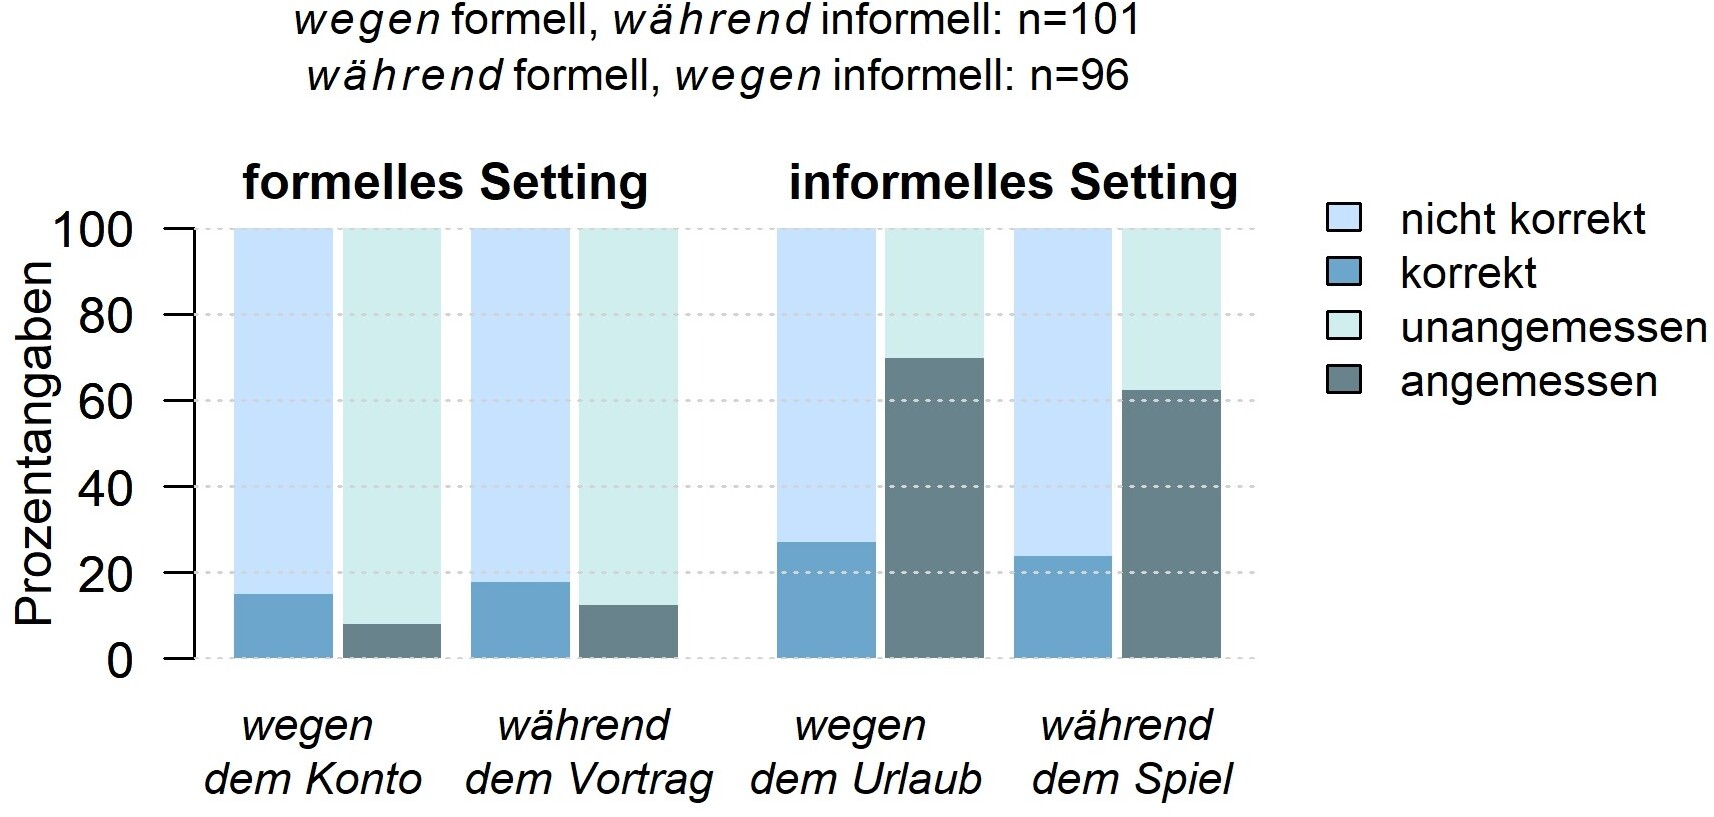
\includegraphics[scale=1]{AkzDativrektion.jpg}
\caption{Akzeptabilität der Dativrektion}
\label{pic:AkzDativrektion}
\end{figure}

Es zeigen sich deutliche Unterschiede zwischen dem formellen und dem informellen Setting. 
Interessanterweise wird dabei nicht nur die Angemessenheit situationsabhängig bewertet, sondern auch die Korrektheit. 
So wird \object{wegen dem Konto} in einem Brief an ein Amt (formelles Setting) nur von 14,9~\% der Befragten dieser Gruppe als korrekt angesehen, in einem Gespräch mit einem Freund (informelles Setting) aber empfinden 27,1~\% \object{wegen dem Urlaub} als richtig. 
Bei \waehrend{} ist der Unterschied geringer: 17,7~\% bewerten \object{während dem Vortrag} im formellen Setting als korrekt und für 23,8~\% ist \object{während dem Spiel} in einem informellen Setting korrekt. 

Große Unterschiede zwischen den beiden Settings ergeben sich in Bezug auf die Angemessenheit. 
Während nur 7,9~\% \wegen{} mit Dativrektion mit Blick auf einen formellen Brief angemessen finden, wird die Form in einem informellen Gespräch von 69,8~\% als angemessen beurteilt. 
Ganz ähnlich fallen die Angemessenheitsurteile bei \waehrend{} aus: Im formellen Brief ist die Dativrektion nur für 12,5~\% angemessen, im informellen Gespräch jedoch für 62,4~\%. 

%Der Unterschied zwischen formellem und informellem Setting wird bei der Beurteilung der Angemessenheit für beide ursprünglichen Genitivpräpositionen hochsignifikant bei mittlerer bis hoher Effektstärke. \\
Auffällig ist die starke Diskrepanz zwischen der Bewertung der Korrektheit und der Angemessenheit im informellen Kontext:
Obwohl die Dativrektion von der Mehrheit als inkorrekte Variante angesehen wird, empfindet eine ähnlich große Mehrheit sie als angemessen. 
Im formellen Kontext ist das Verhältnis zwischen Angemessenheit und Korrektheit umgekehrt: Die Dativrektion wird auch hier selten als korrekt eingestuft, als angemessen wird sie aber sogar noch etwas seltener bewertet. 

Mit dieser zweischichtigen Bewertung bringen die Befragten ihr Wissen um die Indexikalität der Varianten zum Ausdruck. 
Auf der einen Seite wissen sie, dass die Dativrektion bei \wegen{} und \waehrend{} als Fehler stigmatisiert wird, auf der anderen Seite verfügen sie über das Wissen, dass diese Rektionsvariante als informell registriert und in einem Gespräch daher durchaus zu erwarten ist. % Änderung Anfang
Zu berücksichtigen ist dabei, dass eine Diskrepanz zwischen dem Medium der beschriebenen Situation (mündlich) und dem Medium der Präsentation im Fragebogen (schriftlich) vorliegt. 
Es ist denkbar, dass die Dativvarianten bei einer tatsächlich mündlichen Präsentation noch höhere Akzeptabilitätswerte erhalten hätten. % Änderung Ende

\autoref{pic:AkzGenitivrektion} zeigt, inwiefern die Genitivrektion bei den ursprünglichen Dativpräpositionen \dank{} und \gegenueber{} akzeptiert wird (s. zusätzlich \autoref{table:AnhAkzDank} und \autoref{table:AnhAkzGegenueber} im Anhang). 
Vergleicht man die Ergebnisse bei \dank{} zwischen dem formellen und dem informellen Setting, lässt sich Folgendes feststellen: 
Die Genitivrektion bei \dank{} wird sowohl in einem Brief an ein Amt als auch in einer Unterhaltung mit einem Freund überwiegend als korrekt und angemessen eingestuft. 
Jeweils knapp über 90~\% der Befragten empfinden die Variante als korrekt. 
Die Angabe, die Genitivrektion sei unangemessen, wird im informellen Setting nur wenig häufiger getroffen als im formellen.
Damit lässt sich bereits festhalten, dass \dank{} von beinahe allen Befragten als Genitivpräposition angesehen und akzeptiert wird. 
Die Genitivrektion bei \dank{} ist -- anders als die Dativrektion bei \wegen{} und \waehrend{} -- nicht als falsch stigmatisiert und wird daher in beiden Settings gleichermaßen als angemessen empfunden. % Änderung Anfang
Hierbei könnte auch eine Rolle spielen, dass die Präposition \dank{} selbst als formell registriert ist und das Beispiel des informellen Settings daher eventuell weniger informell wahrgenommen wird.% Änderung Ende 
\begin{figure}
\centering
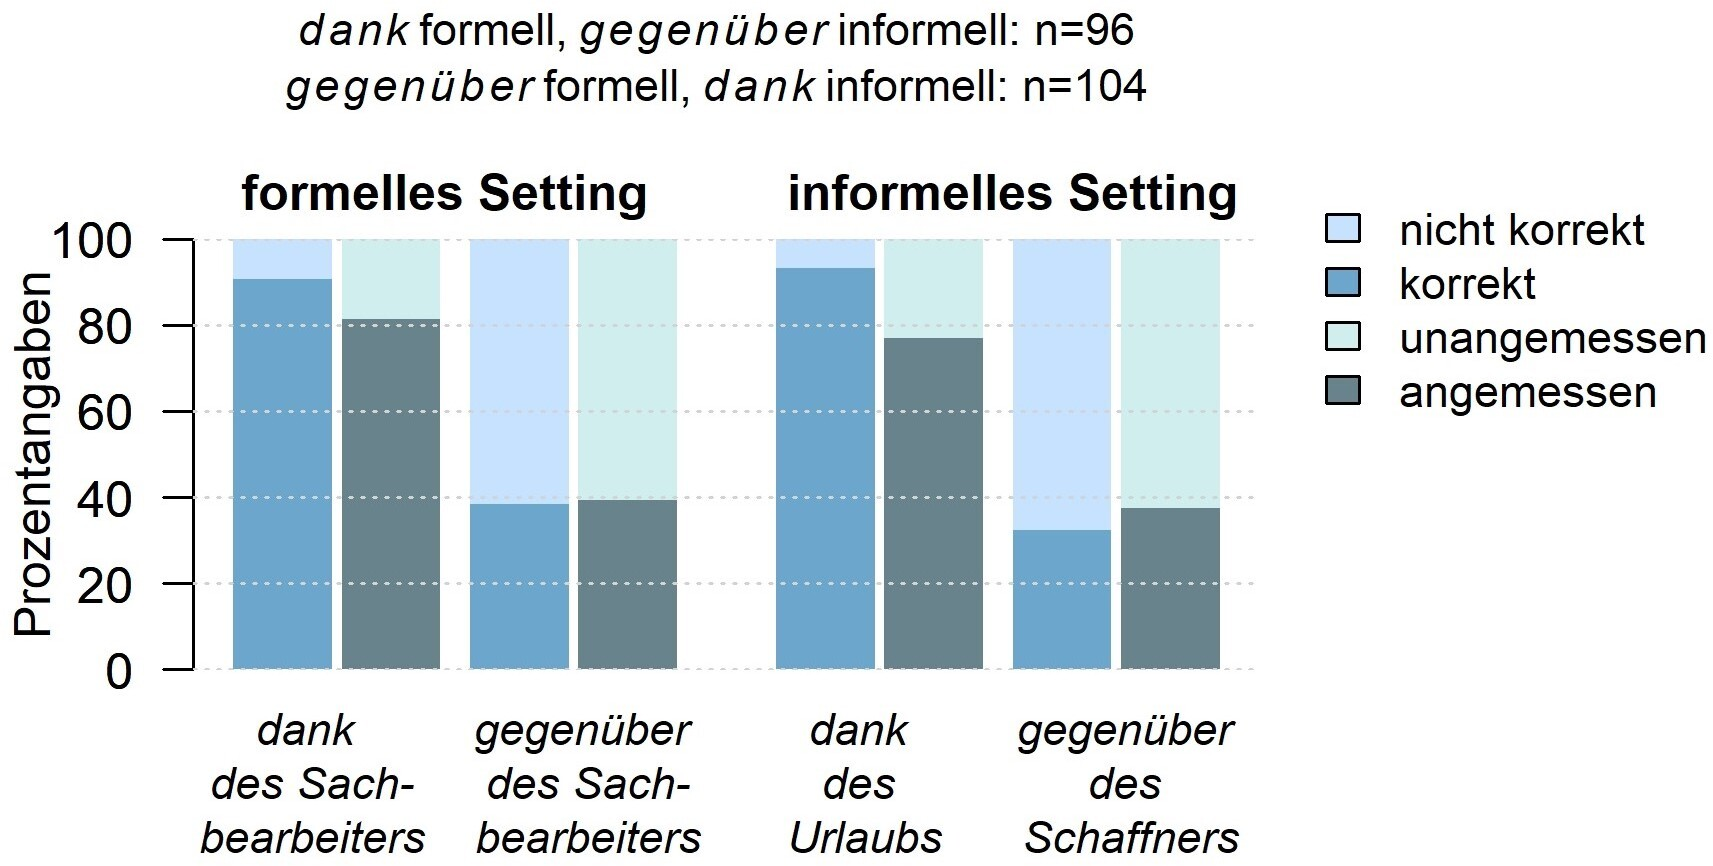
\includegraphics[scale=1]{AkzGenitivrektion.jpg}
\caption{Akzeptabilität der Genitivrektion}
\label{pic:AkzGenitivrektion}
\end{figure}

Obwohl sie laut bisherigen Untersuchungen kaum vorkommt (\autoref{sec:Differenzierung}), wird auch die Genitivrektion bei \gegenueber{} von erstaunlich vielen Befragten als korrekt empfunden:  38,5~\% bewerten  das Beispiel \object{gegenüber des Sachbearbeiters} in einem Brief an ein Amt als korrekt und immerhin 32,3~\% sehen die Genitivrektion bei \object{gegenüber des Schaffners} in einem Gespräch mit einem Freund als korrekt an.

Zwischen den Angaben zur Korrektheit und denen zur Angemessenheit ergeben sich für die Genitivrektion bei \dank{} und \gegenueber{} nur geringe Abweichungen: 
Von den meisten Befragten wird die als korrekt erachtete Form auch als angemessen empfunden bzw. umgekehrt. 

Welche Wirkung das Prestige des Genitivs entfalten kann, zeigt sich auch in den Ergebnissen des Akzeptabilitätstests zur Primärpräposition \object{seit}, die in \autoref{pic:AkzSeitKorrUAng} dargestellt sind (s. außerdem \autoref{table:AnhAkzseit} im Anhang). 
Im formellen Setting beurteilt jeweils beinahe ein Drittel der Befragten \object{seit} mit dem Genitiv als korrekt und angemessen. 
Im informellen Setting wird die Variante immerhin von knapp über 20~\% als korrekt und angemessen eingeschätzt. 
\begin{figure}
\centering
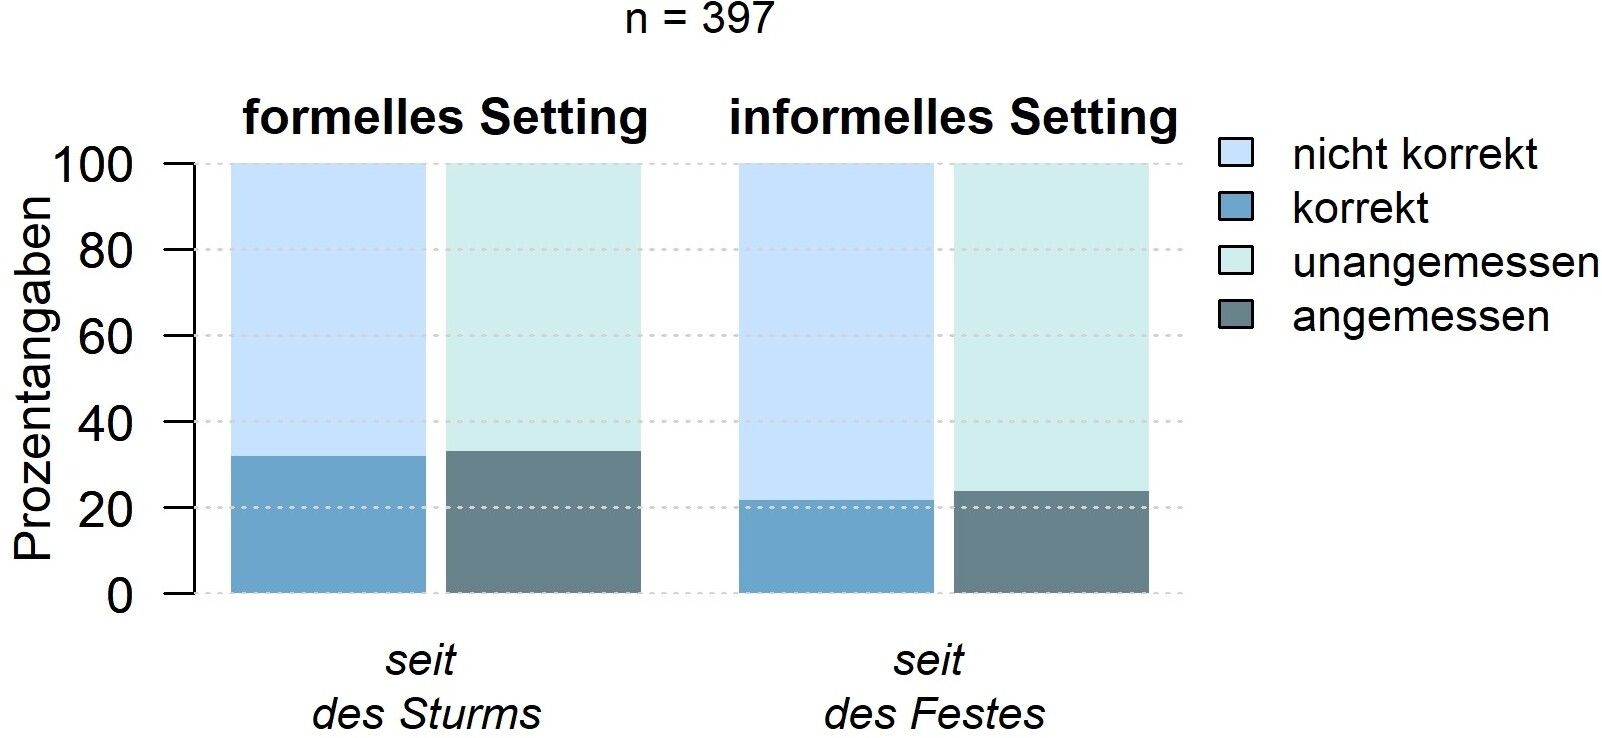
\includegraphics[scale=1]{AkzSeitKorrUAng.jpg}
\caption{Akzeptabilität der Genitivrektion bei der Primärpräposition \object{seit}}
\label{pic:AkzSeitKorrUAng}
\end{figure}

Sowohl die Ergebnisse zu \gegenueber{} als auch die Ergebnisse aus dem in \autoref{sec:Differenzierung} besprochenen Produktionsexperiment von \citet{Becker2011} zeigen, dass Sekundärpräpositionen, die laut kodifizierter Norm ausschließlich mit dem Dativ stehen können, von Befragten häufig mit dem Genitiv akzeptiert werden. 
In \citeauthor{Becker2011}s Experiment verwendeten sogar ca. 65~\% die Genitivrektion bei Präpositionen wie \object{gemäß} oder \object{entsprechend} \citep[s.][210]{Becker2011}. 
Die Ergebnisse zu \object{seit} deuten darauf hin, dass auch Primärpräpositionen, für die die Genitivrektion laut kodifizierter Norm ausgeschlossen ist (\autoref{sec:Primaer}), zu einem gewissen Grad mit dem Genitiv akzeptiert werden. 
Eventuell wird dies dadurch begünstigt, dass die Beispiele (\object{seit des Sturms} und \object{seit des Festes}) als Teile kausaler Sätze interpretiert werden könnten, wodurch \object{seit} semantisch in die Nähe von Genitivpräpositionen wie \wegen{} rückt.\footnote{Für den Hinweis auf diese Erklärungsmöglichkeit danke ich Melitta Gillmann.}
Die Konzepte \glq temporale Abfolge\grq{} und \glq Kausalität\grq{} sind metonymisch miteinander verknüpft: Das Wissen um die zeitliche Abfolge implikatiert eine Ursache-Folge-Beziehung \citep[s.][]{Traugott.1991}.
Die Entwicklung von temporalen zu kausalen Markern ist daher ein häufiger Grammatikalisierungspfad, wie bspw. die Grammatikalisierung von Subjunktionen wie \object{weil} oder \object{nachdem} zeigt \citep[s.][]{Gillmann.2018}. 

%\subsection{Angaben zur eigenen Verwendung von Genitiv- und Dativrektion}
%\label{sec:eigeneVerw}
Neben der Beurteilung von Korrektheit und Angemessenheit wurden im Akzeptabilitätstest auch Angaben dazu erhoben, ob die Befragten die Varianten in der beschriebenen Situation selbst verwenden würden. 
Wie in \autoref{sec:Spracheinstellungsforschung} besprochen, lassen Aussagen zur eigenen Verwendung nicht ohne Weiteres Rückschlüsse darauf zu, inwiefern Befragte eine Variante tatsächlich verwenden. 
Aus diesem Grund enthält der Fragebogen zusätzlich ein Produktionsexperiment.  

\autoref{pic:eigeneVerw} zeigt die Angaben zur eigenen Verwendung für alle im Akzeptabilitätstest präsentierten Varianten, d.\,h. für \dank{} und \gegenueber{} mit der Genitivrektion sowie für \wegen{} und \waehrend{} mit der Dativrektion, jeweils im formellen und im informellen Setting. 
Die Genitivrektion bei \dank{} würden laut eigenen Angaben 70,8~\% (formelles Setting) bzw. 73,1~\% (informelles Setting) selbst verwenden. 
Das sind jeweils etwas weniger Befragte als diejenigen, die angeben, dass diese Variante angemessen sei und deutlich weniger (jeweils ca. 20~\%) als diejenigen, die die Variante als korrekt erachten (vgl. \autoref{pic:AkzGenitivrektion}). 
\object{Gegenüber} mit Genitivrektion erhält wie bereits bei der Beurteilung von Korrektheit und Angemessenheit überraschend hohe Werte: 
31,7~\% geben an, dass sie die Form in einem formellen Brief selbst verwenden würden, und 21,8~\% schätzen, dass sie diese Variante in einer informellen Unterhaltung gebrauchen würden. 
Auch hier liegen die Werte jeweils etwas unter denen zu Korrektheit und Angemessenheit. 
Dass die Anzahl Befragter, die angeben, die Formen selbst zu verwenden, geringer ist als die Anzahl Befragter, die die Formen korrekt oder angemessen finden, deutet evtl. auf Unsicherheiten bei der Beurteilung der Beispiele hin. 
%Inwiefern die Befragten ihren Gebrauch einer Variante evtl. über- oder unterschätzen, wird in \autoref{sec:ProdNachAkz} anhand des Vergleichs mit den Ergebnissen aus dem Produktionsexperiment untersucht. 
\begin{figure}
\centering
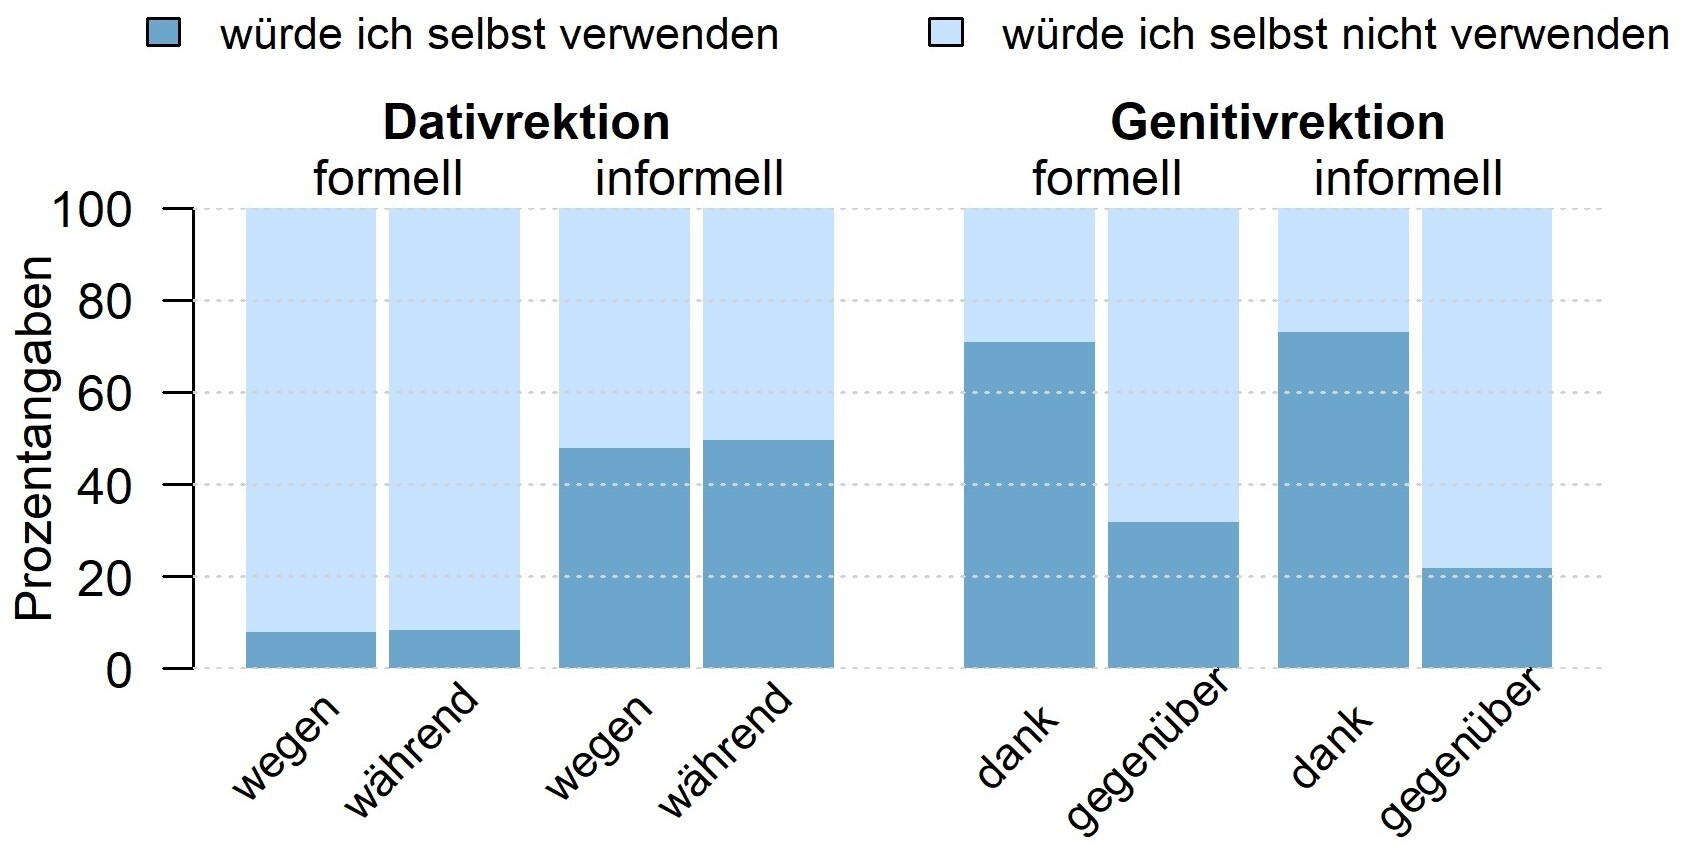
\includegraphics[width=\textwidth]{eigeneVerw.jpg}
\caption{Angaben zur eigenen Verwendung}
\label{pic:eigeneVerw}
\end{figure}

Anders als bei der Genitivrektion zeigen sich bei den Angaben zur eigenen Verwendung der Dativrektion große Unterschiede zwischen dem formellen und dem informellen Setting, wie dies bereits bei der Beurteilung von Korrektheit und Angemessenheit der Fall war. 
Nur 7,9~\% geben an, in einem Brief an ein Amt \wegen{} mit dem Dativ zu verwenden, 8,3~\% sind es bei \waehrend{} mit dem Dativ. 
In einem Gespräch unter Freunden hingegen können sich bei \wegen{} 47,9~\% vorstellen, die Dativrektion zu gebrauchen, bei \waehrend{} 49,5~\%. 
Umgekehrt heißt dies aber auch, dass die Hälfte der Befragten laut eigenen Angaben auch in einer informellen mündlichen Situation den Genitiv mit \wegen{} und \waehrend{} gebrauchen würde, im Falle von \dank{} sogar beinahe drei Viertel. 
Insgesamt schätzen die Befragten also bei Genitivvarianten eher, dass sie diese selbst verwenden würden.
%EVTL NOCH ZUSAMMENFASSENDE ABBILDUNG, IN DER AKZEPTABILITÄT UND VERWENDUNG ZU SEHEN SIND

Die Auswertung der Frage \glqq würden Sie die Variante selbst verwenden?\grqq{} bei \object{seit} mit der Genitivrektion lässt sich \autoref{pic:eigeneVerwSeit} entnehmen. 
Auch bei der Primärpräposition \object{seit} gibt beinahe ein Drittel der Befragten (28~\%) an, die Genitivrektion in einem formellen Brief potenziell selbst zu verwenden. 
Hingegen geben nur ca. 13~\% an, dass sie \object{seit} mit dem Genitiv in einem informellen Gespräch selbst verwenden würden, obwohl über 20~\% die Variante hier als korrekt und angemessen bewerten (s. \autoref{pic:AkzSeitKorrUAng}). 
Auch wenn die Zustimmungswerte für die eigene Verwendung bei \object{seit} geringer sind als bei den anderen Genitivvarianten, muss festgehalten werden, dass sich insbesondere in einem formellen Kontext recht viele Befragte vorstellen können, den Genitiv bei \object{seit} zu verwenden. 
\begin{figure}
\centering
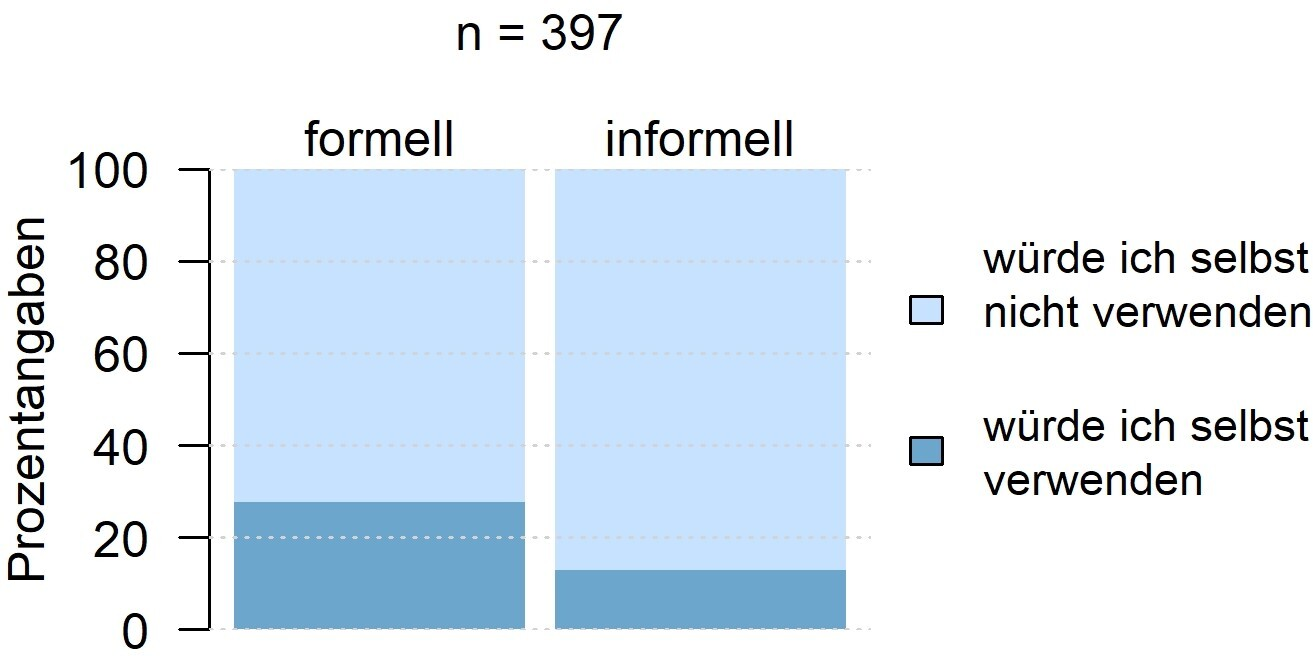
\includegraphics[scale=1]{eigeneVerwSeit.jpg}
\caption{Angaben zur eigenen Verwendung der Primärpräposition \object{seit} mit dem Genitiv}
\label{pic:eigeneVerwSeit}
\end{figure}

Die Auswertung der Angaben zu Korrektheit, Angemessenheit und eigener Verwendung im Vergleich zwischen dem formellen und dem informellen Setting lässt sich folgendermaßen zusammenfassen:
Tendenziell erzielen die Genitivvarianten (\dank{}, \gegenueber{} und \object{seit} plus Genitiv) höhere Akzeptabilitätswerte als die Dativvarianten (\wegen{} und \waehrend{} plus Dativ). 
Die Genitivrektion wird selbst mit der Primärpräposition \object{seit} in beiden Settings von mehr als 20~\% der Befragten als korrekt und angemessen bewertet, während die Dativrektion mit \wegen{} und \waehrend{} im formellen Setting von jeweils unter 20~\% als korrekt oder angemessen eingestuft wird. 
Die Dativrektion bei den ursprünglichen Genitivpräpositionen \wegen{} und \waehrend{} wird kontextabhängig bewertet.
Sie gilt im informellen Setting etwas häufiger als korrekt und deutlich häufiger als angemessen als im formellen Setting. 
Bei der Bewertung der Genitivrektion bei \dank{}, \gegenueber{} und \object{seit} fallen die Unterschiede zwischen den Settings geringer aus.  
Bei allen fünf Präpositionen scheint für die Befragten die Angemessenheit im formellen Setting weitgehend mit der Korrektheit zusammenzufallen, während die Bewertung beider Dimensionen im informellen Setting auseinandergehen kann. 
Die folgenden Abschnitte beschäftigen sich damit, inwiefern sich die Angaben zu Korrektheit, Angemessenheit und der eigenen Verwendung der Varianten in verschiedenen Befragtengruppen unterscheiden. 
\subsection{Akzeptabilität und Alter}
\label{sec:ErgAkzNachAlter}
%Akzeptabilität und Alter
% Änderung!
Da es sich bei Kasusschwankungen von Sekundärpräpositionen um ein Sprachwandelpänomen handelt, ist es entsprechend dem \textit{apparent-time}-Ansatz Labovs eine naheliegende Vermutung, dass sich ältere und jüngere SprachbenutzerInnen in ihrer Bewertung der Varianten unterscheiden (\citealp[s.][40]{Preston.1991}). 
\citet[313]{Bailey.2004} fasst diesen Ansatz wie folgt zusammen:
\begin{quote}Labov hypothesized that when social and stylistic factors were held constant, linguistic differences among different generations of a population (apparent-time differences) would mirror actual diachronic developments in the language (real-time linguistic changes).\end{quote}
% Ende Änderung
Im Folgenden wird daher untersucht, wie die Angaben zu Korrektheit, Angemessenheit und eigener Verwendung der im Akzeptabilitätstest abgefragten Rektionsvarianten mit dem Alter der Befragten zusammenhängen. 
Dafür wird die jüngste Gruppe der Befragten (18 bis 25 Jahre) mit der ältesten Gruppe der Befragten (61 bis 85 Jahre) verglichen. 
Für alle fünf Präpositionen (\wegen{}, \waehrend{}, \dank{}, \gegenueber{} und \object{seit}) werden jeweils die Akzeptabilitätswerte im formellen sowie im informellen Setting betrachtet.

Beim Vergleich der jüngsten mit den ältesten Befragten muss berücksichtigt werden, dass die beiden Altersgruppen sich auch in anderen soziodemografischen Merkmalen unterscheiden (\autoref{sec:Befragte}):
Unter den über 60-jährigen Befragten finden sich mehr Personen ohne Abitur und deutlich mehr Norddeutsche als unter den 18- bis 25-jährigen Befragten.\footnote{Der Anteil an Befragten ohne Hochschulabschluss ist zwar in beiden Altersgruppen etwa gleich, jedoch befinden sich viele der unter 26-jährigen Befragten gerade im Studium und haben dieses noch nicht abgeschlossen (\autoref{sec:Bildung}).} 

Da die BefragungsteilnehmerInnen für den Akzeptabilitätstest auf vier Gruppen verteilt wurden (s. \autoref{table:AkzBsp} und \autoref{sec:Akz}), finden sich pro Gruppe jeweils nur recht wenige Befragte für jede Altersgruppe. 
Aus diesem Grund werden die beiden Gruppen, die im Akzeptabilitätstest die Präpositionen \wegen{} und \waehrend{} bewertet haben, hier zusammen betrachtet. 
%Zur Erinnerung: Die Gruppen unterscheiden sich darin, welche der beiden Präpositionen im informellen Kontext (Gespräch mit einem Freund) und welche im formellen Kontext (Brief an ein Amt) bewertet wurde. 
\object{Wegen} und \waehrend{} gemeinsam zu betrachten, bietet sich an, da beide Präpositionen ein ähnliches sprachhistorisches Profil haben und heute zu einem ähnlichen Maß Rektionsschwankungen zeigen (\autoref{cha:SekPraeps}). 
In beiden Gruppen zusammen sind 51 Befragte zwischen 18 und 25 Jahren und 29 Befragte zwischen 61 und 85 Jahren, wie aus \autoref{table:ErgAkzDativNachAlter} hervorgeht. 
Von den 51 Jüngeren haben dabei 26 \wegen{} plus Dativ im formellen und \waehrend{} plus Dativ im informellen Setting bewertet, 25 beurteilten hingegen \wegen{} plus Dativ im informellen Setting und \waehrend{} plus Dativ im formellen. 
Von den 29 älteren Befragten bewerteten 14 \wegen{} plus Dativ im formellen und \waehrend{} plus Dativ im informellen Setting sowie 15 umgekehrt \wegen{} plus Dativ im informellen Setting und \waehrend{} plus Dativ im formellen.
\autoref{table:ErgAkzDativNachAlter} zeigt die addierten Zahlen beider Gruppen, getrennt nach Altersgruppen. 
Angegeben sind jeweils die absoluten Zahlen sowie die Prozentwerte.\footnote{Aufgrund von Rundungsungenauigkeiten kann es dazu kommen, dass die addierten Prozentwerte nicht genau 100 ergeben.}
Letztere dienen nur der besseren Lesbarkeit beim Vergleich der beiden Gruppen und sind aufgrund der geringen Stichprobengröße mit Vorsicht zu betrachten. 
% Please add the following required packages to your document preamble:
% \usepackage{multirow}
% \usepackage[table,xcdraw]{xcolor}
% If you use beamer only pass "xcolor=table" option, i.e. \documentclass[xcolor=table]{beamer}
\begin{table}
\centering
\begin{tabular}{llrrrr}
\multicolumn{6}{l}{\wegen{} oder \waehrend{} + Dativ nach Alter}                                                                                                                                                                                                                          \\ \hline
                                                                                &                                      & \multicolumn{2}{c}{\begin{tabular}[c]{@{}c@{}}18--25 Jahre\\ (n=51)\end{tabular}} & \multicolumn{2}{c}{\begin{tabular}[c]{@{}c@{}}61--85 Jahre\\ (n=29)\end{tabular}} \\ \hline
                                                                                & \cellcolor[HTML]{9B9B9B}korrekt      & \cellcolor[HTML]{9B9B9B}10          & \cellcolor[HTML]{9B9B9B}{\footnotesize (19,61 \%)}         & \cellcolor[HTML]{9B9B9B}3           & \cellcolor[HTML]{9B9B9B}{\footnotesize (10,34 \%)}         \\ %\cline{2-6} 
                                                                                & \cellcolor[HTML]{9B9B9B}inkorrekt    & \cellcolor[HTML]{9B9B9B}41          & \cellcolor[HTML]{9B9B9B}{\footnotesize (80,39 \%)}         & \cellcolor[HTML]{9B9B9B}26          & \cellcolor[HTML]{9B9B9B}{\footnotesize (89,66 \%)}         \\ %\cline{2-6} 
                                                                                & \cellcolor[HTML]{EFEFEF}angemessen   & \cellcolor[HTML]{EFEFEF}6           & \cellcolor[HTML]{EFEFEF}{\footnotesize (11,76 \%)}         & \cellcolor[HTML]{EFEFEF}1           & \cellcolor[HTML]{EFEFEF}{\footnotesize (3,45 \%)}          \\ %\cline{2-6} 
                                                                                & \cellcolor[HTML]{EFEFEF}unangemessen & \cellcolor[HTML]{EFEFEF}45          & \cellcolor[HTML]{EFEFEF}{\footnotesize (88,24 \%)}         & \cellcolor[HTML]{EFEFEF}28          & \cellcolor[HTML]{EFEFEF}{\footnotesize (96,55 \%)}         \\ %\cline{2-6} 
                                                                                & eigene Verwendung ja                 & 8                                   & {\footnotesize (15,69 \%)}                                 & 0                                   & {\footnotesize (0 \%)}                                     \\ %\cline{2-6} 
\multirow{-6}{*}{\begin{tabular}[c]{@{}l@{}}formelles\\ Setting\end{tabular}}   & eigene Verwendung nein               & 43                                  & {\footnotesize (84,31 \%})                                 & 29                                  & {\footnotesize (100 \%)}                                   \\ \hline
                                                                                &                                      & \multicolumn{2}{c}{\begin{tabular}[c]{@{}c@{}}18--25 Jahre\\ (n=51)\end{tabular}} & \multicolumn{2}{c}{\begin{tabular}[c]{@{}c@{}}61--85 Jahre\\ (n=29)\end{tabular}} \\ \hline
                                                                                & \cellcolor[HTML]{9B9B9B}korrekt      & \cellcolor[HTML]{9B9B9B}15          & \cellcolor[HTML]{9B9B9B}{\footnotesize (29,41 \%)}         & \cellcolor[HTML]{9B9B9B}4           & \cellcolor[HTML]{9B9B9B}{\footnotesize (13,79 \%)}         \\ %\cline{2-6} 
                                                                                & \cellcolor[HTML]{9B9B9B}inkorrekt    & \cellcolor[HTML]{9B9B9B}36          & \cellcolor[HTML]{9B9B9B}{\footnotesize (70,59 \%)}         & \cellcolor[HTML]{9B9B9B}25          & \cellcolor[HTML]{9B9B9B}{\footnotesize (86,21 \%)}         \\ %\cline{2-6} 
                                                                                & \cellcolor[HTML]{EFEFEF}angemessen   & \cellcolor[HTML]{EFEFEF}42          & \cellcolor[HTML]{EFEFEF}{\footnotesize (82,35 \%)}         & \cellcolor[HTML]{EFEFEF}10          & \cellcolor[HTML]{EFEFEF}{\footnotesize (34,48 \%)}         \\ %\cline{2-6} 
                                                                                & \cellcolor[HTML]{EFEFEF}unangemessen & \cellcolor[HTML]{EFEFEF}9           & \cellcolor[HTML]{EFEFEF}{\footnotesize (17,65 \%)}         & \cellcolor[HTML]{EFEFEF}19          & \cellcolor[HTML]{EFEFEF}{\footnotesize (65,52 \%)}         \\ %\cline{2-6} 
                                                                                & eigene Verwendung ja                 & 31                                  & {\footnotesize (60,78 \%)}                                 & 7                                   & {\footnotesize (24,14 \%)}                                 \\ %\cline{2-6} 
\multirow{-6}{*}{\begin{tabular}[c]{@{}l@{}}informelles\\ Setting\end{tabular}} & eigene Verwendung nein               & 20                                  & {\footnotesize (39,22 \%)}                                 & 22                                  & {\footnotesize (75,86 \%)}                                 \\ \hline
\end{tabular}
\caption{Akzeptabilität der Dativrektion bei \wegen{} und \waehrend{} nach Alter}
\label{table:ErgAkzDativNachAlter}
\end{table}

Der größte Unterschied zwischen den jüngeren und den älteren Befragten ist die Bewertung der Angemessenheit im informellen Setting: 
Die deutliche Mehrheit der Befragten zwischen 18 und 25 empfindet die Dativrektion bei \wegen{} oder \waehrend{} als angemessen (42 von 51). 
Nur ein Drittel der älteren Befragten teilt diese Einschätzung (zehn von 29). 
Auch die Angaben zur eigenen Verwendung unterscheiden sich deutlich. 
Während eine Mehrheit der jüngeren Befragten den Dativ in einem informellen Kontext verwenden würde (31 von 51), gibt nur eine Minderheit der älteren Befragten an, dies zu tun (sieben von 29). 
In beiden Altersgruppen zeigen dich Unterschiede zwischen der Akzeptabilität im formellen und im informellen Setting, jedoch sind diese in der Gruppe der 18- bis 25-Jährigen größer.
Die jüngere Gruppe scheint also etwas kontextsensitiver zu sein als die ältere Gruppe. 
Auch die Diskrepanz zwischen der Bewertung der Korrektheit und der Bewertung der Angemessenheit ist in der Gruppe der jüngeren Befragten größer als unter den über 60-Jährigen. 

Um mögliche Altersunterschiede bei der Akzeptabilität der Genitivrektion zu identifizieren, wird zunächst nur die Präposition \dank{} betrachtet (s. \autoref{table:ErgAkzDankNachAlter}). 
Die Ergebnisse zu \dank{} mit denen zu \gegenueber{} zusammenzurechnen, wird vermieden, da diese beiden Präpositionen zu verschieden sind: 
Während der Genitiv bei \dank{} bereits etabliert ist, kommt er bei \gegenueber{} noch kaum vor (\autoref{cha:SekPraeps}). 
Die Stichproben sind hier daher deutlich kleiner als bei der Betrachtung der Akzeptabilität der Dativrektion. 
Dies liegt an der vom Zufallsmechanismus des Fragebogens vorgenommenen Gruppeneinteilung. 
In die Gruppe, die \dank{} plus Genitiv im formellen Setting bewertete, wurden vom Zufallsgenerator 29 Befragte zwischen 18 und 25 und neun Befragte über 60 eingeteilt. 
Im informellen Setting bewerteten 24 jüngere und neun ältere Befragte \dank{} plus Genitiv. 
Die Zahlen in \autoref{table:ErgAkzDankNachAlter} lassen kaum nennenswerte Unterschiede zwischen jüngeren und älteren Befragten erkennen. 
Zwar lehnt unter den Befragten über 60 ein größerer Anteil \dank{} plus Genitiv im informellen Kontext als unangemessen ab, jedoch lässt sich dies aufgrund der geringen Zahlen nicht interpretieren. 
% Please add the following required packages to your document preamble:
% \usepackage{multirow}
% \usepackage[table,xcdraw]{xcolor}
% If you use beamer only pass "xcolor=table" option, i.e. \documentclass[xcolor=table]{beamer}
\begin{table}
\centering
\begin{tabular}{llrrrr}
\multicolumn{6}{l}{\dank{} + Genitiv nach Alter}                                                                                                                                                                                                                                      \\ \hline
                                                                                &                                      & \multicolumn{2}{c}{\begin{tabular}[c]{@{}c@{}}18--25 Jahre\\ (n=29)\end{tabular}} & \multicolumn{2}{c}{\begin{tabular}[c]{@{}c@{}}61--85 Jahre\\ (n=9)\end{tabular}} \\ \hline
                                                                                & \cellcolor[HTML]{9B9B9B}korrekt      & \cellcolor[HTML]{9B9B9B}28          & \cellcolor[HTML]{9B9B9B}{\footnotesize (96,55 \%)}         & \cellcolor[HTML]{9B9B9B}8          & \cellcolor[HTML]{9B9B9B}{\footnotesize (88,89 \%)}         \\ %\cline{2-6} 
                                                                                & \cellcolor[HTML]{9B9B9B}inkorrekt    & \cellcolor[HTML]{9B9B9B}1           & \cellcolor[HTML]{9B9B9B}{\footnotesize (3,45 \%)}          & \cellcolor[HTML]{9B9B9B}1          & \cellcolor[HTML]{9B9B9B}{\footnotesize (11,11 \%)}         \\ %\cline{2-6} 
                                                                                & \cellcolor[HTML]{EFEFEF}angemessen   & \cellcolor[HTML]{EFEFEF}25          & \cellcolor[HTML]{EFEFEF}{\footnotesize (86,21 \%)}         & \cellcolor[HTML]{EFEFEF}6          & \cellcolor[HTML]{EFEFEF}{\footnotesize (66,67 \%)}         \\ %\cline{2-6} 
                                                                                & \cellcolor[HTML]{EFEFEF}unangemessen & \cellcolor[HTML]{EFEFEF}4           & \cellcolor[HTML]{EFEFEF}{\footnotesize (13,79 \%)}         & \cellcolor[HTML]{EFEFEF}3          & \cellcolor[HTML]{EFEFEF}{\footnotesize (33,33 \%)}         \\ %\cline{2-6} 
                                                                                & eigene Verwendung ja                 & 24                                  & {\footnotesize (82,76 \%)}                                 & 6                                  & {\footnotesize (66,67 \%)}                                 \\ %\cline{2-6} 
\multirow{-6}{*}{\begin{tabular}[c]{@{}l@{}}formelles\\ Setting\end{tabular}}   & eigene Verwendung nein               & 5                                   & {\footnotesize (17,24 \%)}                                 & 3                                  & {\footnotesize (33,33 \%)}                                 \\ \hline
                                                                                &                                      & \multicolumn{2}{c}{\begin{tabular}[c]{@{}c@{}}18--25 Jahre\\ (n=24)\end{tabular}} & \multicolumn{2}{c}{\begin{tabular}[c]{@{}c@{}}61--85 Jahre\\ (n=9)\end{tabular}} \\ \hline
                                                                                & \cellcolor[HTML]{9B9B9B}korrekt      & \cellcolor[HTML]{9B9B9B}21          & \cellcolor[HTML]{9B9B9B}{\footnotesize (87,5 \%)}          & \cellcolor[HTML]{9B9B9B}7          & \cellcolor[HTML]{9B9B9B}{\footnotesize (77,78 \%)}         \\ %\cline{2-6} 
                                                                                & \cellcolor[HTML]{9B9B9B}inkorrekt    & \cellcolor[HTML]{9B9B9B}3           & \cellcolor[HTML]{9B9B9B}{\footnotesize (12,5 \%)}          & \cellcolor[HTML]{9B9B9B}2          & \cellcolor[HTML]{9B9B9B}{\footnotesize (22,22 \%)}         \\ %\cline{2-6} 
                                                                                & \cellcolor[HTML]{EFEFEF}angemessen   & \cellcolor[HTML]{EFEFEF}19          & \cellcolor[HTML]{EFEFEF}{\footnotesize (79,17 \%)}         & \cellcolor[HTML]{EFEFEF}5          & \cellcolor[HTML]{EFEFEF}{\footnotesize (55,56 \%)}         \\ %\cline{2-6} 
                                                                                & \cellcolor[HTML]{EFEFEF}unangemessen & \cellcolor[HTML]{EFEFEF}5           & \cellcolor[HTML]{EFEFEF}{\footnotesize (20,83 \%)}         & \cellcolor[HTML]{EFEFEF}4          & \cellcolor[HTML]{EFEFEF}{\footnotesize (44,44 \%)}         \\ %\cline{2-6} 
                                                                                & eigene Verwendung ja                 & 18                                  & {\footnotesize (75 \%)}                                    & 6                                  & {\footnotesize (66,67 \%)}                                 \\ %\cline{2-6} 
\multirow{-6}{*}{\begin{tabular}[c]{@{}l@{}}informelles\\ Setting\end{tabular}} & eigene Verwendung nein               & 6                                   & {\footnotesize (25 \%)}                                    & 3                                  & {\footnotesize (33,33 \%)}                                 \\ \hline
\end{tabular}
\caption{Akzeptabilität der Genitivrektion bei dank nach Alter}
\label{table:ErgAkzDankNachAlter}
\end{table}

Die Genitivrektion bei \gegenueber{} wurde im formellen Setting von 24 Befragten aus der jüngsten und neun Befragten aus der ältesten Altersgruppe bewertet. 
Im informellen Setting bekamen diese Variante aufgrund des Zufallsgenerators 29 Befragte zwischen 18 und 25 und neun Befragte über 60. 
Betrachtet man die Akzeptabilität der Genitivrektion bei \gegenueber{} in den beiden Altersgruppen, lassen sich mögliche Unterschiede im formellen Setting erkennen (s. \autoref{table:ErgAkzGegenueberNachAlter}). 
Jeweils ca. die Hälfte der insgesamt 24 18- bis 25-jährigen Befragten empfindet die Variante als korrekt und angemessen und würde sie selbst verwenden. 
Acht von neun über 60-Jährigen lehnen sie hingegen als inkorrekt ab, alle neun bewerten sie als unangemessen. 
% Please add the following required packages to your document preamble:
% \usepackage{multirow}
% \usepackage[table,xcdraw]{xcolor}
% If you use beamer only pass "xcolor=table" option, i.e. \documentclass[xcolor=table]{beamer}
\begin{table}
\centering
\begin{tabular}{llrrrr}
\multicolumn{6}{l}{\gegenueber{} + Genitiv nach Alter}                                                                                                                                                                                                                                \\ \hline
                                                                                &                                      & \multicolumn{2}{c}{\begin{tabular}[c]{@{}c@{}}18--25 Jahre\\ (n=24)\end{tabular}} & \multicolumn{2}{c}{\begin{tabular}[c]{@{}c@{}}61--85 Jahre\\ (n=9)\end{tabular}} \\ \hline
                                                                                & \cellcolor[HTML]{9B9B9B}korrekt      & \cellcolor[HTML]{9B9B9B}12          & \cellcolor[HTML]{9B9B9B}{\footnotesize (50 \%)}            & \cellcolor[HTML]{9B9B9B}1          & \cellcolor[HTML]{9B9B9B}{\footnotesize (11,11 \%)}         \\ %\cline{2-6} 
                                                                                & \cellcolor[HTML]{9B9B9B}inkorrekt    & \cellcolor[HTML]{9B9B9B}12          & \cellcolor[HTML]{9B9B9B}{\footnotesize (50 \%)}            & \cellcolor[HTML]{9B9B9B}8          & \cellcolor[HTML]{9B9B9B}{\footnotesize (88,89 \%)}         \\ %\cline{2-6} 
                                                                                & \cellcolor[HTML]{EFEFEF}angemessen   & \cellcolor[HTML]{EFEFEF}11          & \cellcolor[HTML]{EFEFEF}{\footnotesize (45,83 \%)}         & \cellcolor[HTML]{EFEFEF}0          & \cellcolor[HTML]{EFEFEF}{\small (0 \%)}             \\ %\cline{2-6} 
                                                                                & \cellcolor[HTML]{EFEFEF}unangemessen & \cellcolor[HTML]{EFEFEF}13          & \cellcolor[HTML]{EFEFEF}{\footnotesize (54,17 \%)}         & \cellcolor[HTML]{EFEFEF}9          & \cellcolor[HTML]{EFEFEF}{\footnotesize (100 \%)}           \\ %\cline{2-6} 
                                                                                & eigene Verwendung ja                 & 11                                  & {\footnotesize (45,83 \%)}                                 & 0                                  & {\footnotesize (0 \%)}                                     \\ %\cline{2-6} 
\multirow{-6}{*}{\begin{tabular}[c]{@{}l@{}}formelles\\ Setting\end{tabular}}   & eigene Verwendung nein               & 13                                  & {\footnotesize (54,17 \%)}                                 & 9                                  & {\footnotesize (100 \%)}                                   \\ \hline
                                                                                &                                      & \multicolumn{2}{c}{\begin{tabular}[c]{@{}c@{}}18--25 Jahre\\ (n=29)\end{tabular}} & \multicolumn{2}{c}{\begin{tabular}[c]{@{}c@{}}61--85 Jahre\\ (n=9)\end{tabular}} \\ \hline
                                                                                & \cellcolor[HTML]{9B9B9B}korrekt      & \cellcolor[HTML]{9B9B9B}13          & \cellcolor[HTML]{9B9B9B}{\footnotesize (44,83 \%)}         & \cellcolor[HTML]{9B9B9B}4          & \cellcolor[HTML]{9B9B9B}{\footnotesize (44,44 \%)}         \\ %\cline{2-6} 
                                                                                & \cellcolor[HTML]{9B9B9B}inkorrekt    & \cellcolor[HTML]{9B9B9B}16          & \cellcolor[HTML]{9B9B9B}{\footnotesize (55,17 \%)}         & \cellcolor[HTML]{9B9B9B}5          & \cellcolor[HTML]{9B9B9B}{\footnotesize (55,56 \%)}         \\ %\cline{2-6} 
                                                                                & \cellcolor[HTML]{EFEFEF}angemessen   & \cellcolor[HTML]{EFEFEF}13          & \cellcolor[HTML]{EFEFEF}{\footnotesize (44,83 \%)}         & \cellcolor[HTML]{EFEFEF}3          & \cellcolor[HTML]{EFEFEF}{\footnotesize (33,33 \%)}         \\ %\cline{2-6} 
                                                                                & \cellcolor[HTML]{EFEFEF}unangemessen & \cellcolor[HTML]{EFEFEF}16          & \cellcolor[HTML]{EFEFEF}{\footnotesize (55,17 \%)}         & \cellcolor[HTML]{EFEFEF}6          & \cellcolor[HTML]{EFEFEF}{\footnotesize (66,67 \%)}         \\ %\cline{2-6} 
                                                                                & eigene Verwendung ja                 & 6                                   & {\footnotesize (20,69 \%)}                                 & 3                                  & {\footnotesize (33,33 \%)}                                 \\ %\cline{2-6} 
\multirow{-6}{*}{\begin{tabular}[c]{@{}l@{}}informelles\\ Setting\end{tabular}} & eigene Verwendung nein               & 23                                  & {\footnotesize (79,31 \%)}                                 & 6                                  & {\footnotesize (66,67 \%)}                                 \\ \hline
\end{tabular}
\caption{Akzeptabilität der Genitivrektion bei \gegenueber{} nach Alter}
\label{table:ErgAkzGegenueberNachAlter}
\end{table}
%\begin{figure}
%\centering
%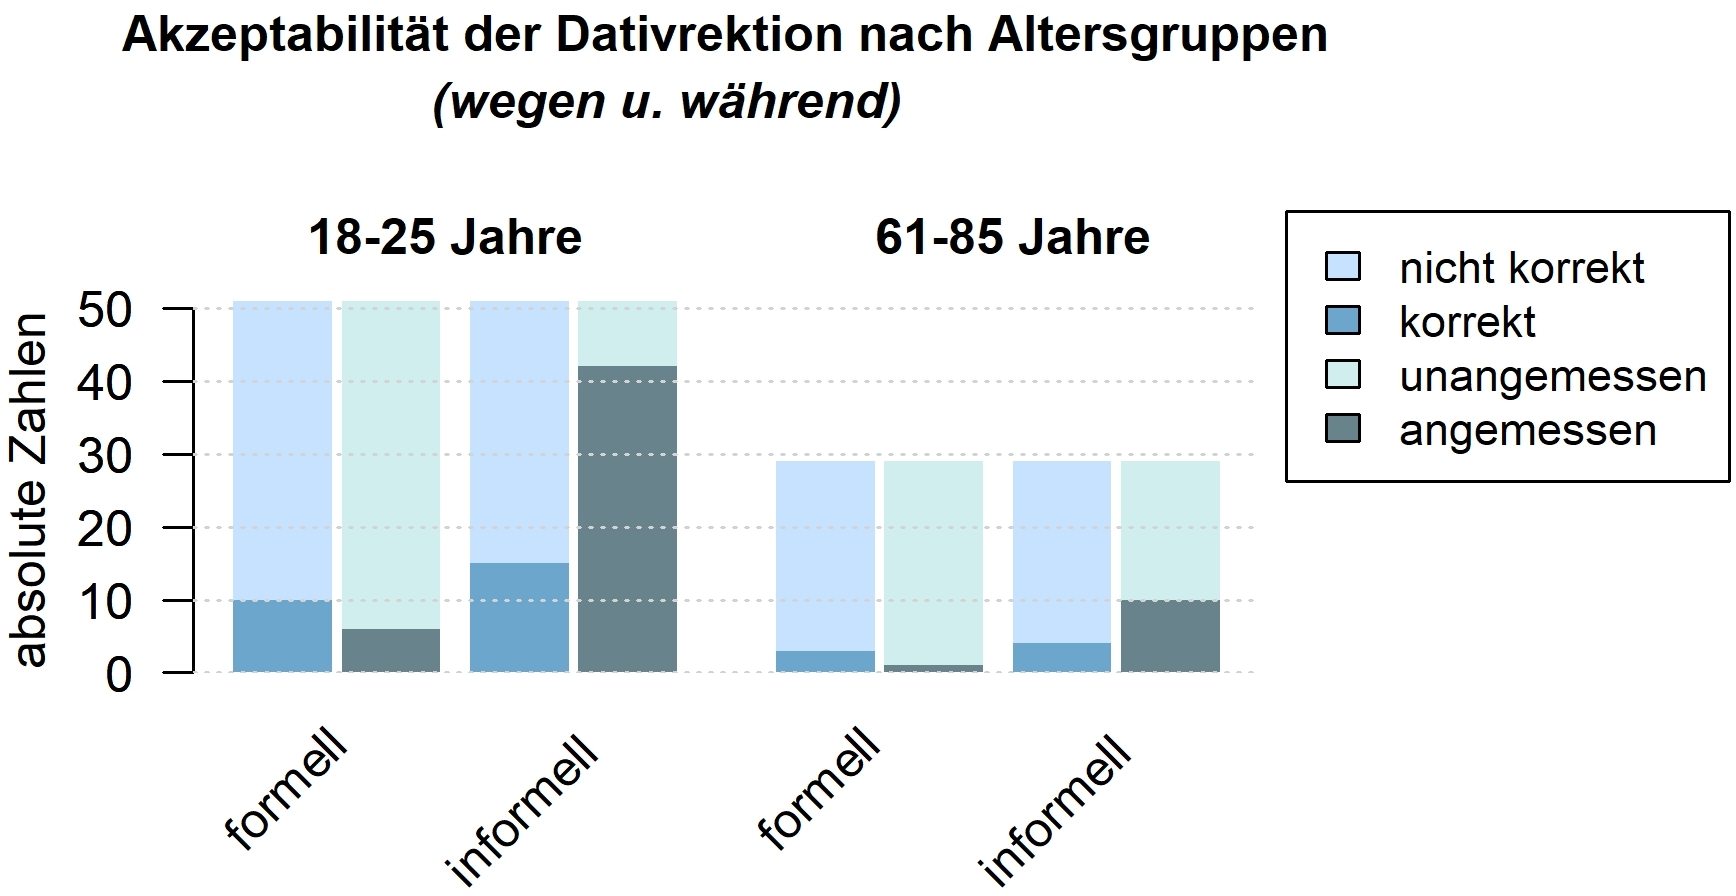
\includegraphics[scale=1]{AkzDativNachAlter.jpg}
%\caption{Akzeptabilität der Dativrektion bei \wegen{} und \waehrend{} nach Altersgruppen}
%\label{pic:AkzDativNachAlter}
%\end{figure}
%\begin{figure}
%\centering
%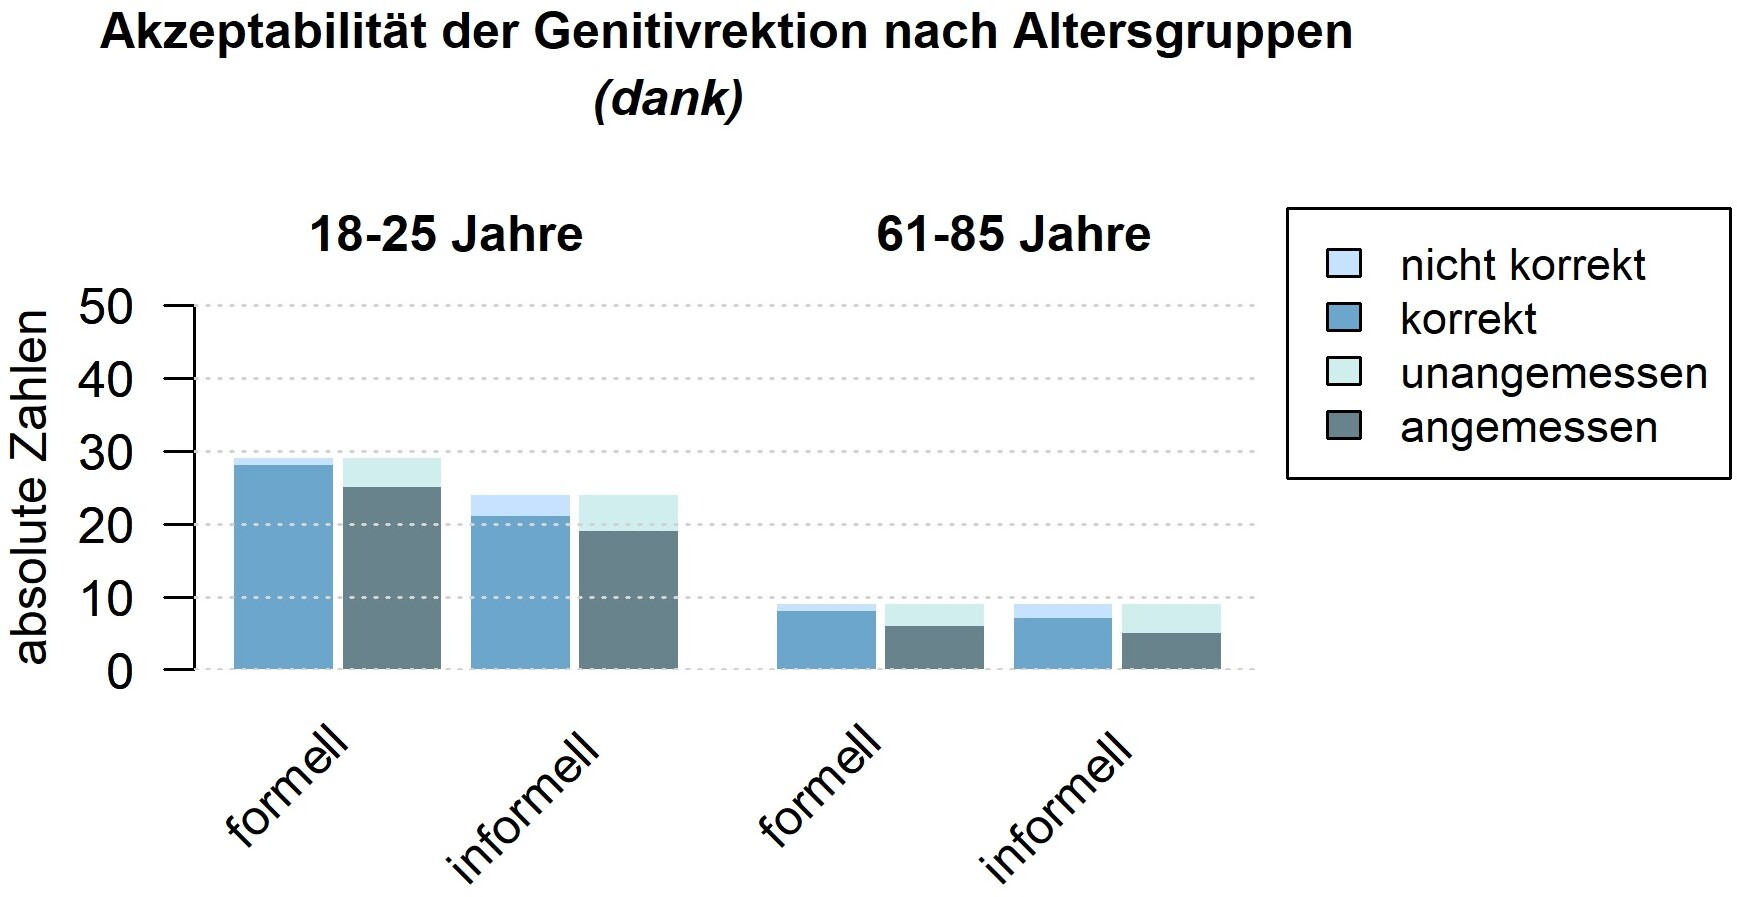
\includegraphics[scale=1]{AkzGenitivNachAlter.jpg}
%\caption{Akzeptabilität der Genitivrektion bei \dank{} nach Altersgruppen}
%\label{pic:AkzGenitivNachAlter}
%\end{figure}

Wie oben erläutert, bewerteten alle Befragten im Akzeptabilitätstest zusätzlich die Primärpräposition \object{seit} mit dem Genitiv. 
Abschließend werden daher die Akzeptabilitätswerte der Genitivrektion bei \object{seit} in den beiden Altersgruppen verglichen (s. \autoref{table:ErgAkzSeitNachAlter}).
In der Gruppe der 18- bis 25-Jährigen befinden sich insgesamt 104 Befragte, in der Gruppe der 61- bis 85-Jährigen 47. 
Im formellen Setting zeigen sich kaum Unterschiede zwischen den Altersgruppen.
Im informellen Setting bewerten unter den älteren Befragten jeweils weniger \object{seit} plus Genitiv als korrekt und angemessen. 
Dass sie die Form selbst verwenden würden, geben aus beiden Altersgruppen jedoch ähnlich viele an. 
% Please add the following required packages to your document preamble:
% \usepackage{multirow}
% \usepackage[table,xcdraw]{xcolor}
% If you use beamer only pass "xcolor=table" option, i.e. \documentclass[xcolor=table]{beamer}
\begin{table}
\centering
\begin{tabular}{llrrrr}
\multicolumn{6}{l}{\object{seit} + Genitiv nach Alter}                                                                                                                                                                                                                                            \\ \hline
                                                                                &                                      & \multicolumn{2}{c}{\begin{tabular}[c]{@{}c@{}}18--25 Jahre\\ (n=104)\end{tabular}} & \multicolumn{2}{c}{\begin{tabular}[c]{@{}c@{}}61--85 Jahre\\ (n=47)\end{tabular}} \\ \hline
                                                                                & \cellcolor[HTML]{9B9B9B}korrekt      & \cellcolor[HTML]{9B9B9B}32         & \cellcolor[HTML]{9B9B9B}{\footnotesize (30,77 \%)}        & \cellcolor[HTML]{9B9B9B}13         & \cellcolor[HTML]{9B9B9B}{\footnotesize (27,66 \%)}        \\ %\cline{2-6} 
                                                                                & \cellcolor[HTML]{9B9B9B}inkorrekt    & \cellcolor[HTML]{9B9B9B}72         & \cellcolor[HTML]{9B9B9B}{\footnotesize (69,23 \%)}        & \cellcolor[HTML]{9B9B9B}34         & \cellcolor[HTML]{9B9B9B}{\footnotesize (72,34 \%)}        \\ %\cline{2-6} 
                                                                                & \cellcolor[HTML]{EFEFEF}angemessen   & \cellcolor[HTML]{EFEFEF}32         & \cellcolor[HTML]{EFEFEF}{\footnotesize (30,77 \%)}        & \cellcolor[HTML]{EFEFEF}12         & \cellcolor[HTML]{EFEFEF}{\footnotesize (25,53 \%)}        \\ %\cline{2-6} 
                                                                                & \cellcolor[HTML]{EFEFEF}unangemessen & \cellcolor[HTML]{EFEFEF}72         & \cellcolor[HTML]{EFEFEF}{\footnotesize (69,23 \%)}        & \cellcolor[HTML]{EFEFEF}35         & \cellcolor[HTML]{EFEFEF}{\footnotesize (74,47 \%)}        \\ %\cline{2-6} 
                                                                                & eigene Verwendung ja                 & 27                                 & {\footnotesize (25,96 \%)}                                & 11                                 & {\footnotesize (23,4 \%)}                                 \\ %\cline{2-6} 
\multirow{-6}{*}{\begin{tabular}[c]{@{}l@{}}formelles\\ Setting\end{tabular}}   & eigene Verwendung nein               & 77                                 & {\footnotesize (74,04 \%)}                                & 36                                 & {\footnotesize (76,6 \%)}                                 \\ \hline
                                                                                &                                      & \multicolumn{2}{c}{\begin{tabular}[c]{@{}c@{}}18--25 Jahre\\ (n=104)\end{tabular}} & \multicolumn{2}{c}{\begin{tabular}[c]{@{}c@{}}61--85 Jahre\\ (n=47)\end{tabular}} \\ \hline
                                                                                & \cellcolor[HTML]{9B9B9B}korrekt      & \cellcolor[HTML]{9B9B9B}28         & \cellcolor[HTML]{9B9B9B}{\footnotesize (26,92 \%)}        & \cellcolor[HTML]{9B9B9B}7          & \cellcolor[HTML]{9B9B9B}{\footnotesize (14,89 \%)}        \\ %\cline{2-6} 
                                                                                & \cellcolor[HTML]{9B9B9B}inkorrekt    & \cellcolor[HTML]{9B9B9B}76         & \cellcolor[HTML]{9B9B9B}{\footnotesize (73,08 \%)}        & \cellcolor[HTML]{9B9B9B}40         & \cellcolor[HTML]{9B9B9B}{\footnotesize (85,11 \%)}        \\ %\cline{2-6} 
                                                                                & \cellcolor[HTML]{EFEFEF}angemessen   & \cellcolor[HTML]{EFEFEF}27         & \cellcolor[HTML]{EFEFEF}{\footnotesize (25,96 \%)}        & \cellcolor[HTML]{EFEFEF}7          & \cellcolor[HTML]{EFEFEF}{\footnotesize (14,89 \%)}        \\ %\cline{2-6} 
                                                                                & \cellcolor[HTML]{EFEFEF}unangemessen & \cellcolor[HTML]{EFEFEF}77         & \cellcolor[HTML]{EFEFEF}{\footnotesize (74,04 \%)}        & \cellcolor[HTML]{EFEFEF}40         & \cellcolor[HTML]{EFEFEF}{\footnotesize (85,11 \%)}        \\ %\cline{2-6} 
                                                                                & eigene Verwendung ja                 & 12                                 & {\footnotesize (11,54 \%)}                                & 7                                  & {\footnotesize (14,89 \%)}                                \\ %\cline{2-6} 
\multirow{-6}{*}{\begin{tabular}[c]{@{}l@{}}informelles\\ Setting\end{tabular}} & eigene Verwendung nein               & 92                                 & {\footnotesize (88,46 \%)}                               & 40                                 & {\footnotesize (85,11 \%)}                                \\ \hline
\end{tabular}
\caption{Akzeptabilität der Genitivrektion bei \object{seit} nach Alter}
\label{table:ErgAkzSeitNachAlter}
\end{table}

Der Vergleich der beiden Altersgruppen deutet darauf hin, dass ältere und jüngere SprachbenutzerInnen die Dativrektion bei \wegen{} und \waehrend{} und die Genitivrektion bei \dank{} ähnlich bewerten. 
In der Beurteilung der Angemessenheit im informellen Kontext zeigen sich aber jeweils Unterschiede, hier scheinen die Jüngeren offener gegenüber dem Dativ zu sein. 
Bei \wegen{} und \waehrend{} geben sie auch häufiger an, die Dativrektion in einem informellen Kontext selbst zu verwenden. 
Dass die älteren Befragten den Dativ bei \wegen{}, \waehrend{} und \dank{} weniger zu akzeptieren scheinen, könnte jedoch dadurch bedingt sein, dass in dieser Gruppe deutlich mehr Norddeutsche sind. 
Bei \gegenueber{} plus Genitiv deuten sich Unterschiede im formellen Setting an:
Während ca. die Hälfte der jüngeren Befragten die Variante akzeptiert, wird sie von beinahe allen älteren Befragten abgelehnt. 
Aufgrund der geringen Stichprobengröße kann es sich allerdings auch um zufällige Unterschiede handeln. 
Die Genitivrektion bei der Primärpräposition \object{seit} wird im informellen Kontext von der älteren Befragtengruppe etwas seltener als korrekt und angemessen bewertet als von der jüngeren. 
\subsection{Akzeptabilität und regionale Herkunft}
\label{sec:ErgAkzNachRegion}
% Akzeptabilität und regionale Herkunft
Die in \autoref{sec:KorpusstudienRektion} vorgestellten Korpusstudien zur regionalen Verteilung der Rektionsvarianten lassen vermuten, dass der Dativ in süddeutschen Bundesländern akzeptierter ist als in norddeutschen. 
Dies soll nun anhand der Daten aus dem Akzeptabilitätstest überprüft werden. 
Hierfür werden die Befragten aus norddeutschen Bundesländern (Bremen, Hamburg, Niedersachsen und Schleswig-Holstein) den Befragten aus süddeutschen Bundesländern (Bayern oder Baden-Württemberg) gegenübergestellt. 
Dabei ist zu berücksichtigen, dass unter den norddeutschen Befragten der Anteil von Personen über 60 deutlich höher ist (22~\%) als unter den süddeutschen Befragten (3~\%, s. \autoref{sec:HerkunftundDialekt}). 
Wieder werden zunächst \wegen{} und \waehrend{} gemeinsam betrachtet, anschließend \dank{}, \gegenueber{} und \object{seit} jeweils einzeln. 

\autoref{table:ErgAkzDativNachHerkunft} zeigt die summierten Akzeptabilitätswerte für \wegen{} und \waehrend{} mit dem Dativ, aufgeteilt nach regionaler Herkunft. 
Insgesamt wurden die beiden ursprünglichen Genitivpräpositionen von 81 Befragten aus Norddeutschland und 46 Befragten aus Süddeutschland bewertet. 
Diese regionalen Gruppen setzen sich wie folgt zusammen: 
Von den 81 norddeutschen Befragten sind 41 in der Gruppe, die die Akzeptabilität von \wegen{} plus Dativ im formellen und diejenige von \waehrend{} plus Dativ im informellen Kontext bewertete.
40 Norddeutsche erhielten umgekehrt \waehrend{} im formellen und \wegen{} im informellen Kontext zur Beurteilung. 
Von den 46 süddeutschen Befragten finden sich in der ersten Gruppe 19 und in der zweiten Gruppe 27. 
% Please add the following required packages to your document preamble:
% \usepackage{multirow}
% \usepackage[table,xcdraw]{xcolor}
% If you use beamer only pass "xcolor=table" option, i.e. \documentclass[xcolor=table]{beamer}
\begin{table}
\centering
\begin{tabular}{llrrrr}
\multicolumn{6}{l}{\wegen{} oder \waehrend{} + Dativ nach regionaler Herkunft}                                                                                                                                                                                                                                 \\ \hline
                                                                                &                                      & \multicolumn{2}{c}{\begin{tabular}[c]{@{}c@{}}Norddeutschland\\ (n=81)\end{tabular}} & \multicolumn{2}{c}{\begin{tabular}[c]{@{}c@{}}Süddeutschland\\ (n=46)\end{tabular}} \\ \hline
                                                                                & \cellcolor[HTML]{9B9B9B}korrekt      & \cellcolor[HTML]{9B9B9B}13            & \cellcolor[HTML]{9B9B9B}{\footnotesize (16,05 \%)}           & \cellcolor[HTML]{9B9B9B}13           & \cellcolor[HTML]{9B9B9B}{\footnotesize (28,26 \%)}           \\ %\cline{2-6} 
                                                                                & \cellcolor[HTML]{9B9B9B}inkorrekt    & \cellcolor[HTML]{9B9B9B}68            & \cellcolor[HTML]{9B9B9B}{\footnotesize (83,95 \%)}           & \cellcolor[HTML]{9B9B9B}33           & \cellcolor[HTML]{9B9B9B}{\footnotesize (71,74 \%)}           \\ %\cline{2-6} 
                                                                                & \cellcolor[HTML]{EFEFEF}angemessen   & \cellcolor[HTML]{EFEFEF}8             & \cellcolor[HTML]{EFEFEF}{\footnotesize (9,88 \%)}            & \cellcolor[HTML]{EFEFEF}6            & \cellcolor[HTML]{EFEFEF}{\footnotesize (13,04 \%)}           \\ %\cline{2-6} 
                                                                                & \cellcolor[HTML]{EFEFEF}unangemessen & \cellcolor[HTML]{EFEFEF}73            & \cellcolor[HTML]{EFEFEF}{\footnotesize (90,12 \%)}           & \cellcolor[HTML]{EFEFEF}40           & \cellcolor[HTML]{EFEFEF}{\footnotesize (86,96 \%)}           \\ %\cline{2-6} 
                                                                                & eigene Verwendung ja                 & 5                                     & {\footnotesize (6,17 \%)}                                    & 8                                    & {\footnotesize (17,39 \%)}                                   \\ %\cline{2-6} 
\multirow{-6}{*}{\begin{tabular}[c]{@{}l@{}}formelles\\ Setting\end{tabular}}   & eigene Verwendung nein               & 76                                    & {\footnotesize (93,83 \%)}                                   & 38                                   & {\footnotesize (82,61 \%)}                                   \\ \hline
                                                                                &                                      & \multicolumn{2}{c}{\begin{tabular}[c]{@{}c@{}}Norddeutschland\\ (n=81)\end{tabular}} & \multicolumn{2}{c}{\begin{tabular}[c]{@{}c@{}}Süddeutschland\\ (n=46)\end{tabular}} \\ \hline
                                                                                & \cellcolor[HTML]{9B9B9B}korrekt      & \cellcolor[HTML]{9B9B9B}11            & \cellcolor[HTML]{9B9B9B}{\footnotesize (13,58 \%)}           & \cellcolor[HTML]{9B9B9B}22           & \cellcolor[HTML]{9B9B9B}{\footnotesize (47,83 \%)}           \\ %\cline{2-6} 
                                                                                & \cellcolor[HTML]{9B9B9B}inkorrekt    & \cellcolor[HTML]{9B9B9B}70            & \cellcolor[HTML]{9B9B9B}{\footnotesize (86,42 \%)}           & \cellcolor[HTML]{9B9B9B}24           & \cellcolor[HTML]{9B9B9B}{\footnotesize (52,17 \%)}           \\ %\cline{2-6} 
                                                                                & \cellcolor[HTML]{EFEFEF}angemessen   & \cellcolor[HTML]{EFEFEF}39            & \cellcolor[HTML]{EFEFEF}{\footnotesize (48,15 \%)}           & \cellcolor[HTML]{EFEFEF}41           & \cellcolor[HTML]{EFEFEF}{\footnotesize (89,13 \%)}           \\ %\cline{2-6} 
                                                                                & \cellcolor[HTML]{EFEFEF}unangemessen & \cellcolor[HTML]{EFEFEF}42            & \cellcolor[HTML]{EFEFEF}{\footnotesize (51,85 \%)}           & \cellcolor[HTML]{EFEFEF}5            & \cellcolor[HTML]{EFEFEF}{\footnotesize (10,87 \%)}           \\ %\cline{2-6} 
                                                                                & eigene Verwendung ja                 & 22                                    & {\footnotesize (27,16 \%)}                                   & 38                                   & {\footnotesize (82,61 \%)}                                   \\ %\cline{2-6} 
\multirow{-6}{*}{\begin{tabular}[c]{@{}l@{}}informelles\\ Setting\end{tabular}} & eigene Verwendung nein               & 59                                    & {\footnotesize (72,84 \%)}                                   & 8                                    & {\footnotesize (17,39 \%)}                                   \\ \hline
\end{tabular}
\caption{Akzeptabilität der Dativrektion bei \wegen{} oder \waehrend{} nach regionaler Herkunft}
\label{table:ErgAkzDativNachHerkunft}
\end{table}

Im informellen Kontext akzeptieren die süddeutschen BefragungsteilnehmerInnen den Dativ eher als die norddeutschen. 
Ungefähr die Hälfte der 46 Befragten aus Süddeutschland beurteilt die Dativrektion bei \wegen{} oder \waehrend{} als korrekt, im Norden tun dies hingegen nur elf von 81. 
Nur fünf Befragte aus Süddeutschland bewerten den Dativ im informellen Setting als unangemessen, acht würden ihn selbst nicht verwenden. 
Im Norden hingegen wird die Dativrektion bei \wegen{} oder \waehrend{} in einem informellen Kontext nur von ca. der Hälfte als angemessen empfunden (39 von 81) und nur ca. ein Viertel würde sie selbst verwenden. 
 Die Gruppe, die im Akzeptabilitätstest \dank{} mit dem Genitiv im formellen Setting beurteilt und \gegenueber{} mit dem Genitiv im informellen, umfasst 42 Befragte aus Norddeutschland und 27 Befragte aus Süddeutschland (s. \autoref{table:ErgAkzDankNachHerkunft} und \autoref{table:ErgAkzGegenueberNachHerkunft}).
49 Norddeutsche und 27 Süddeutsche bewerteten \dank{} im informellen und \gegenueber{} im formellen Setting. 
Beide ursprünglichen Dativpräpositionen werden auch hier wieder getrennt behandelt. 
% Please add the following required packages to your document preamble:
% \usepackage{multirow}
% \usepackage[table,xcdraw]{xcolor}
% If you use beamer only pass "xcolor=table" option, i.e. \documentclass[xcolor=table]{beamer}
\begin{table}
\centering
\begin{tabular}{llrrrr}
\multicolumn{6}{l}{\dank{} + Genitiv nach regionaler Herkunft}                                                                                                                                                                                                                                \\ \hline
                                                                                &                                      & \multicolumn{2}{c}{\begin{tabular}[c]{@{}c@{}}Norddeutschland\\ (n=42)\end{tabular}} & \multicolumn{2}{c}{\begin{tabular}[c]{@{}c@{}}Süddeutschland\\ (n=27)\end{tabular}} \\ \hline
                                                                                & \cellcolor[HTML]{9B9B9B}korrekt      & \cellcolor[HTML]{9B9B9B}37            & \cellcolor[HTML]{9B9B9B}{\footnotesize (88,1 \%)}            & \cellcolor[HTML]{9B9B9B}26           & \cellcolor[HTML]{9B9B9B}{\footnotesize (96,3 \%)}            \\ %\cline{2-6} 
                                                                                & \cellcolor[HTML]{9B9B9B}inkorrekt    & \cellcolor[HTML]{9B9B9B}5             & \cellcolor[HTML]{9B9B9B}{\footnotesize (11,9 \%})            & \cellcolor[HTML]{9B9B9B}1            & \cellcolor[HTML]{9B9B9B}{\footnotesize (3,7 \%})             \\ %\cline{2-6} 
                                                                                & \cellcolor[HTML]{EFEFEF}angemessen   & \cellcolor[HTML]{EFEFEF}32            & \cellcolor[HTML]{EFEFEF}{\footnotesize (76,19 \%)}           & \cellcolor[HTML]{EFEFEF}23           & \cellcolor[HTML]{EFEFEF}{\footnotesize (85,19 \%)}           \\ %\cline{2-6} 
                                                                                & \cellcolor[HTML]{EFEFEF}unangemessen & \cellcolor[HTML]{EFEFEF}10            & \cellcolor[HTML]{EFEFEF}{\footnotesize (23,81 \%)}           & \cellcolor[HTML]{EFEFEF}4            & \cellcolor[HTML]{EFEFEF}{\footnotesize (14,81 \%)}           \\ %\cline{2-6} 
                                                                                & eigene Verwendung ja                 & 26                                    & {\footnotesize (61,9 \%)}                                    & 22                                   & {\footnotesize (81,48 \%)}                                   \\ %\cline{2-6} 
\multirow{-6}{*}{\begin{tabular}[c]{@{}l@{}}formelles\\ Setting\end{tabular}}   & eigene Verwendung nein               & 16                                    & {\footnotesize (38,1 \%)}                                    & 5                                    & {\footnotesize (18,52 \%)}                                   \\ \hline
                                                                                &                                      & \multicolumn{2}{c}{\begin{tabular}[c]{@{}c@{}}Norddeutschland\\ (n=49)\end{tabular}} & \multicolumn{2}{c}{\begin{tabular}[c]{@{}c@{}}Süddeutschland\\ (n=27)\end{tabular}} \\ \hline
                                                                                & \cellcolor[HTML]{9B9B9B}korrekt      & \cellcolor[HTML]{9B9B9B}47            & \cellcolor[HTML]{9B9B9B}{\footnotesize (95,92 \%)}           & \cellcolor[HTML]{9B9B9B}26           & \cellcolor[HTML]{9B9B9B}{\footnotesize (96,3 \%)}            \\ %\cline{2-6} 
                                                                                & \cellcolor[HTML]{9B9B9B}inkorrekt    & \cellcolor[HTML]{9B9B9B}2             & \cellcolor[HTML]{9B9B9B}{\footnotesize (4,08 \%)}            & \cellcolor[HTML]{9B9B9B}1            & \cellcolor[HTML]{9B9B9B}{\footnotesize (3,7 \%)}             \\ %\cline{2-6} 
                                                                                & \cellcolor[HTML]{EFEFEF}angemessen   & \cellcolor[HTML]{EFEFEF}38            & \cellcolor[HTML]{EFEFEF}{\footnotesize (77,55 \%)}           & \cellcolor[HTML]{EFEFEF}20           & \cellcolor[HTML]{EFEFEF}{\footnotesize (74,07 \%)}           \\ %\cline{2-6} 
                                                                                & \cellcolor[HTML]{EFEFEF}unangemessen & \cellcolor[HTML]{EFEFEF}11            & \cellcolor[HTML]{EFEFEF}{\footnotesize (22,45 \%)}           & \cellcolor[HTML]{EFEFEF}7            & \cellcolor[HTML]{EFEFEF}{\footnotesize (25,93 \%)}           \\ %\cline{2-6} 
                                                                                & eigene Verwendung ja                 & 38                                    & {\footnotesize (77,55 \%)}                                   & 16                                   & {\footnotesize (59,26 \%)}                                   \\ %\cline{2-6} 
\multirow{-6}{*}{\begin{tabular}[c]{@{}l@{}}informelles\\ Setting\end{tabular}} & eigene Verwendung nein               & 11                                    & {\footnotesize (22,45 \%)}                                   & 11                                   & {\footnotesize (40,74 \%)}                                   \\ \hline
\end{tabular}
\caption{Akzeptabilität der Genitivrektion bei \dank{} nach regionaler Herkunft}
\label{table:ErgAkzDankNachHerkunft}
\end{table}

Die Korrektheit und die Angemessenheit der Genitivrektion bei \dank{} bewerten norddeutsche und süddeutsche Befragte recht ähnlich.
Unterschiede zeigen sich aber in den Angaben zur eigenen Verwendung: 
Im formellen Setting ist der Anteil derer, die \dank{} plus Genitiv verwenden würden, in Süddeutschland deutlich höher als in Norddeutschland. 
Im informellen Setting ist es umgekehrt: Hier würden nur 16 von 27 Befragten aus Süddeutschland den Genitiv verwenden, jedoch 38 von 49 norddeutschen Befragten. 

Die Genitivrektion bei \gegenueber{} wird im informellen Setting von süddeutschen Befragten recht häufig akzeptiert (s. \autoref{table:ErgAkzGegenueberNachHerkunft}): 
Ungefähr die Hälfte (jeweils 13 von 27) stuft \gegenueber{} plus Genitiv in einem Gespräch mit einem Freund als korrekt und angemessen ein. 
Unter den norddeutschen Befragten ist der Anteil deutlich geringer (neun bzw. 14 von 42). 
% Please add the following required packages to your document preamble:
% \usepackage{multirow}
% \usepackage[table,xcdraw]{xcolor}
% If you use beamer only pass "xcolor=table" option, i.e. \documentclass[xcolor=table]{beamer}
\begin{table}
\centering
\begin{tabular}{llrrrr}
\multicolumn{6}{l}{\gegenueber{} + Genitiv nach regionaler Herkunft}                                                                                                                                                                                                                          \\ \hline
                                                                                &                                      & \multicolumn{2}{c}{\begin{tabular}[c]{@{}c@{}}Norddeutschland\\ (n=49)\end{tabular}} & \multicolumn{2}{c}{\begin{tabular}[c]{@{}c@{}}Süddeutschland\\ (n=27)\end{tabular}} \\ \hline
                                                                                & \cellcolor[HTML]{9B9B9B}korrekt      & \cellcolor[HTML]{9B9B9B}19            & \cellcolor[HTML]{9B9B9B}{\footnotesize (38,78 \%)}           & \cellcolor[HTML]{9B9B9B}8            & \cellcolor[HTML]{9B9B9B}{\footnotesize (29,63 \%)}           \\ %\cline{2-6} 
                                                                                & \cellcolor[HTML]{9B9B9B}inkorrekt    & \cellcolor[HTML]{9B9B9B}30            & \cellcolor[HTML]{9B9B9B}{\footnotesize (61,22 \%})           & \cellcolor[HTML]{9B9B9B}19           & \cellcolor[HTML]{9B9B9B}{\footnotesize (70,37 \%)}           \\ %\cline{2-6} 
                                                                                & \cellcolor[HTML]{EFEFEF}angemessen   & \cellcolor[HTML]{EFEFEF}18            & \cellcolor[HTML]{EFEFEF}{\footnotesize (36,73 \%)}           & \cellcolor[HTML]{EFEFEF}9            & \cellcolor[HTML]{EFEFEF}{\footnotesize (33,33 \%)}           \\ %\cline{2-6} 
                                                                                & \cellcolor[HTML]{EFEFEF}unangemessen & \cellcolor[HTML]{EFEFEF}31            & \cellcolor[HTML]{EFEFEF}{\footnotesize (63,27 \%)}           & \cellcolor[HTML]{EFEFEF}18           & \cellcolor[HTML]{EFEFEF}{\footnotesize (66,67 \%)}           \\ %\cline{2-6} 
                                                                                & eigene Verwendung ja                 & 14                                    & {\footnotesize (28,57 \%)}                                   & 8                                    & {\footnotesize (29,63 \%)}                                   \\ %\cline{2-6} 
\multirow{-6}{*}{\begin{tabular}[c]{@{}l@{}}formelles\\ Setting\end{tabular}}   & eigene Verwendung nein               & 35                                    & {\footnotesize (71,43 \%)}                                   & 19                                   & {\footnotesize (70,37 \%)}                                   \\ \hline
                                                                                &                                      & \multicolumn{2}{c}{\begin{tabular}[c]{@{}c@{}}Norddeutschland\\ (n=42)\end{tabular}} & \multicolumn{2}{c}{\begin{tabular}[c]{@{}c@{}}Süddeutschland\\ (n=27)\end{tabular}} \\ \hline
                                                                                & \cellcolor[HTML]{9B9B9B}korrekt      & \cellcolor[HTML]{9B9B9B}9             & \cellcolor[HTML]{9B9B9B}{\footnotesize (21,43 \%)}           & \cellcolor[HTML]{9B9B9B}13           & \cellcolor[HTML]{9B9B9B}{\footnotesize (48,15 \%)}           \\ %\cline{2-6} 
                                                                                & \cellcolor[HTML]{9B9B9B}inkorrekt    & \cellcolor[HTML]{9B9B9B}33            & \cellcolor[HTML]{9B9B9B}{\footnotesize (78,57 \%)}           & \cellcolor[HTML]{9B9B9B}14           & \cellcolor[HTML]{9B9B9B}{\footnotesize (51,85 \%)}           \\ %\cline{2-6} 
                                                                                & \cellcolor[HTML]{EFEFEF}angemessen   & \cellcolor[HTML]{EFEFEF}14            & \cellcolor[HTML]{EFEFEF}{\footnotesize (33,33 \%)}           & \cellcolor[HTML]{EFEFEF}13           & \cellcolor[HTML]{EFEFEF}{\footnotesize (48,15 \%)}           \\ %\cline{2-6} 
                                                                                & \cellcolor[HTML]{EFEFEF}unangemessen & \cellcolor[HTML]{EFEFEF}28            & \cellcolor[HTML]{EFEFEF}{\footnotesize (66,67 \%)}           & \cellcolor[HTML]{EFEFEF}14           & \cellcolor[HTML]{EFEFEF}{\footnotesize (51,85 \%)}           \\ %\cline{2-6} 
                                                                                & eigene Verwendung ja                 & 8                                     & {\footnotesize (19,05 \%)}                                   & 8                                    & {\footnotesize (29,63 \%)}                                   \\ %\cline{2-6} 
\multirow{-6}{*}{\begin{tabular}[c]{@{}l@{}}informelles\\ Setting\end{tabular}} & eigene Verwendung nein               & 34                                    & {\footnotesize (80,95 \%)}                                   & 19                                   & {\footnotesize (70,37 \%)}                                   \\ \hline
\end{tabular}
\caption{Akzeptabilität der Genitivrektion bei \gegenueber{} nach regionaler Herkunft}
\label{table:ErgAkzGegenueberNachHerkunft}
\end{table}
%\begin{figure}
%\centering
%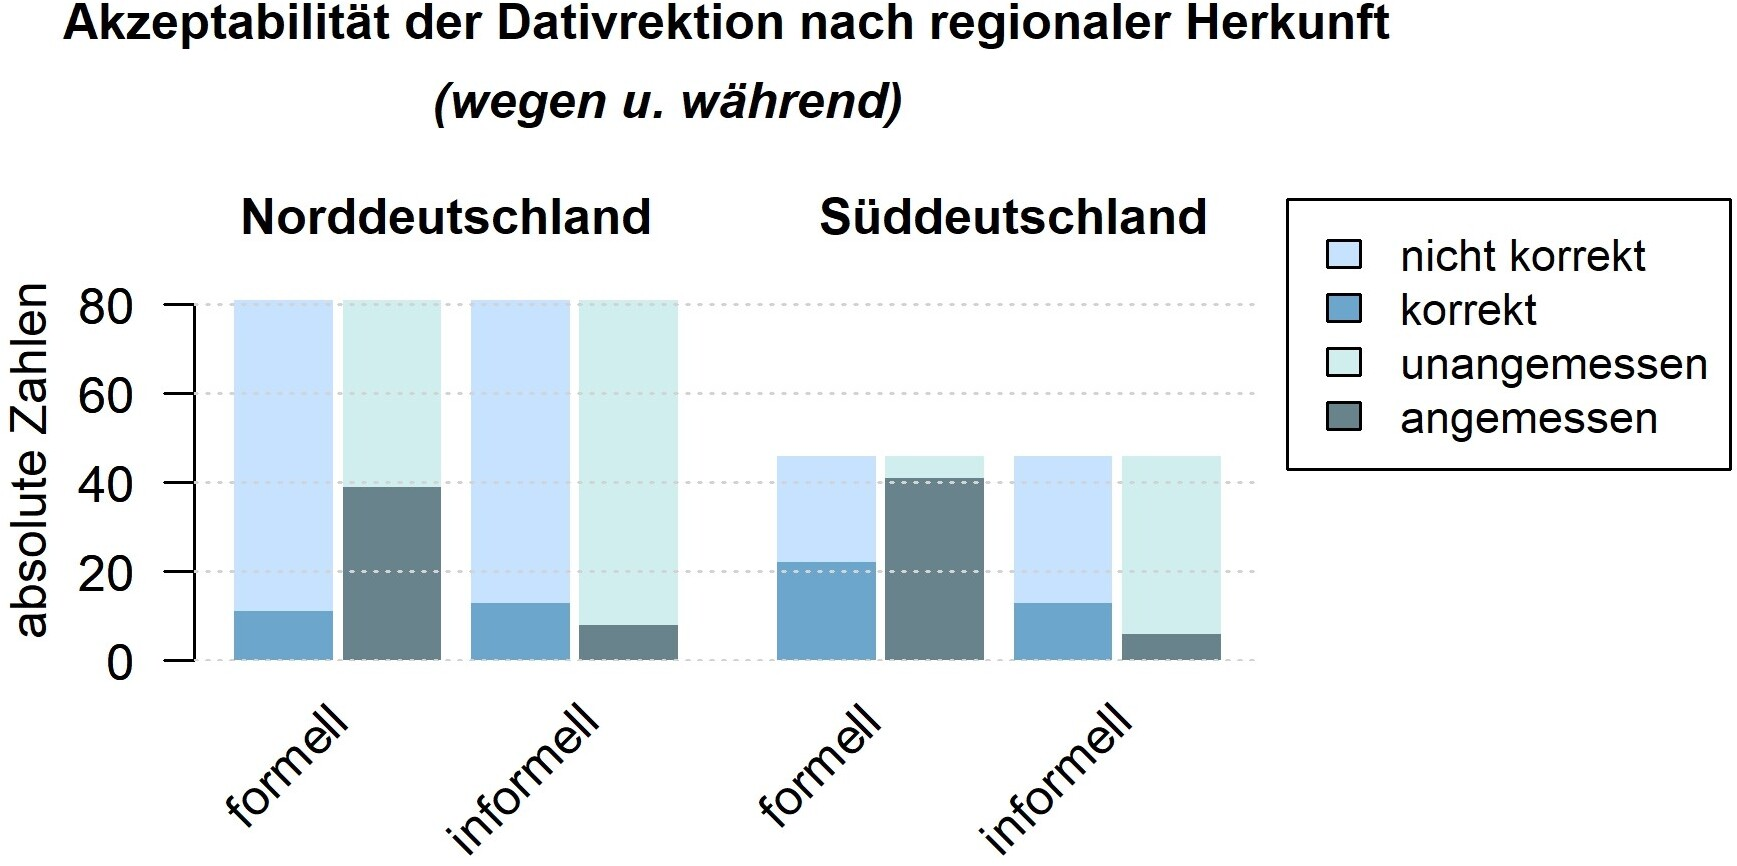
\includegraphics[scale=1]{AkzDativNachRegion.jpg}
%\caption{Akzeptabilität der Dativrektion bei \wegen{} und \waehrend{} nach regionaler Herkunft}
%\label{pic:AkzDativNachRegion}
%\end{figure}
%\begin{figure}
%\centering
%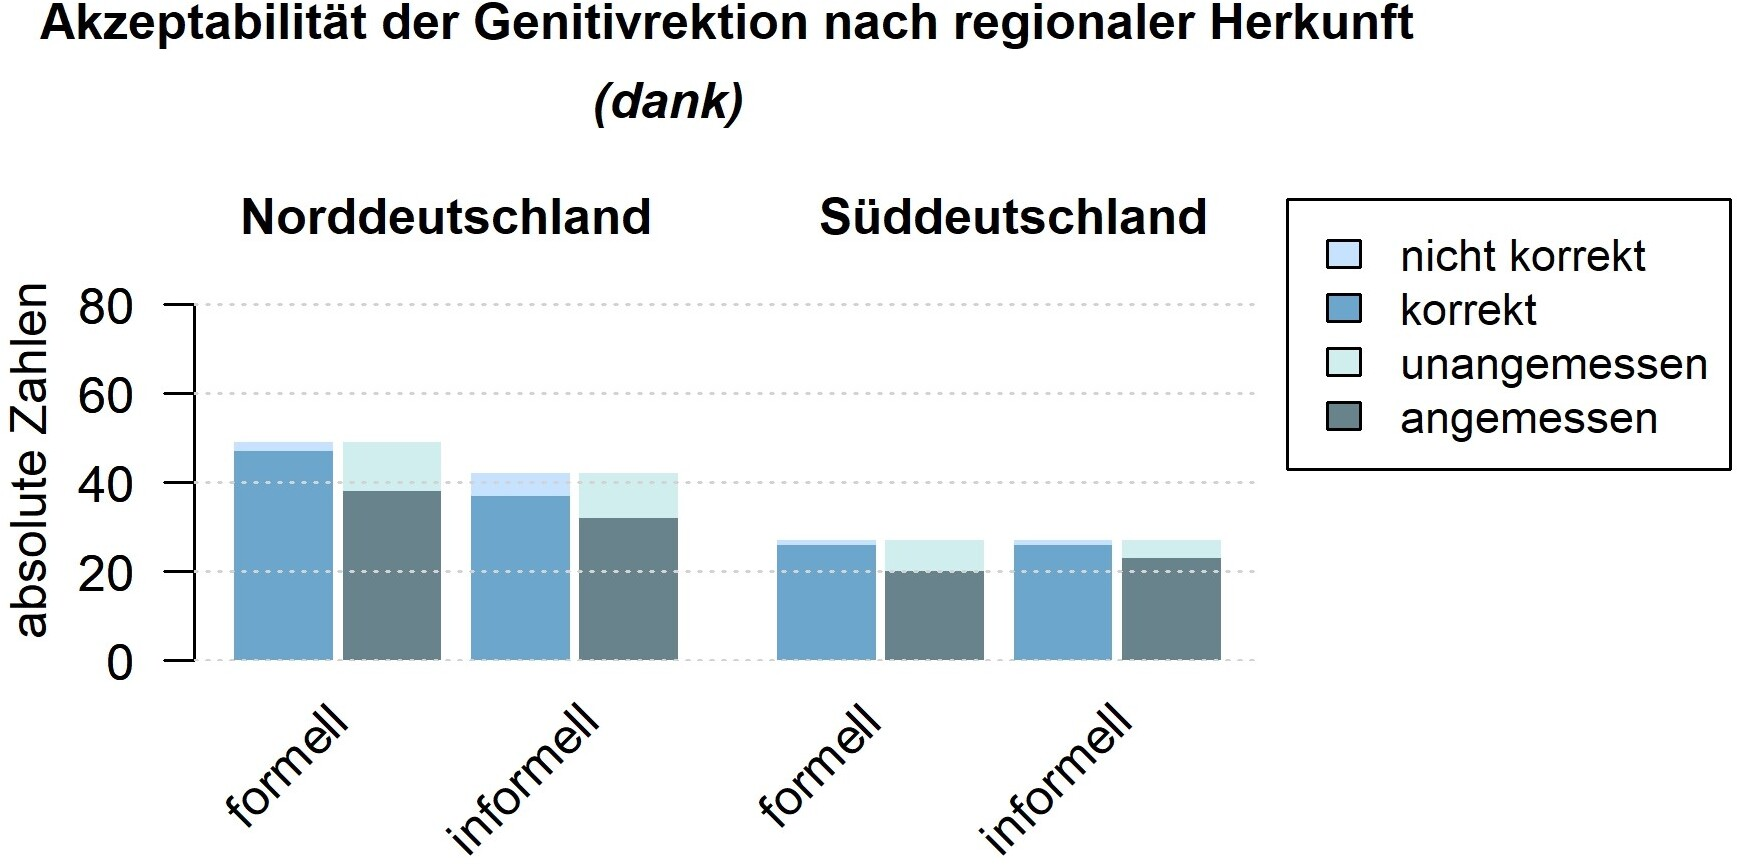
\includegraphics[scale=1]{AkzGenitivNachRegion.jpg}
%\caption{Akzeptabilität der Genitivrektion bei \dank{} nach regionaler Herkunft}
%\label{pic:AkzGenitivNachRegion}
%\end{figure}
% Please add the following required packages to your document preamble:
% \usepackage{multirow}
% \usepackage[table,xcdraw]{xcolor}
% If you use beamer only pass "xcolor=table" option, i.e. \documentclass[xcolor=table]{beamer}

Die Akzeptabilitätswerte der Genitivrektion bei der Primärpräposition \object{seit} sind im Norden (172 Befragte) und Süden (100 Befragte) ähnlich (s. \autoref{table:ErgAkzSeitNachHerkunft}).
Das gilt sowohl für das formelle als auch für das informelle Setting. 
Lediglich die Frage danach, ob sie die Variante selbst verwenden würden, wird unter den süddeutschen Befragten noch etwas häufiger verneint. 
\begin{table}
\centering
\begin{tabular}{llrrrr}
\multicolumn{6}{l}{\object{seit} + Genitiv nach regionaler Herkunft}                                                                                                                                                                                                                                  \\ \hline
                                                                                &                                      & \multicolumn{2}{c}{\begin{tabular}[c]{@{}c@{}}Norddeutschland\\ (n=172)\end{tabular}} & \multicolumn{2}{c}{\begin{tabular}[c]{@{}c@{}}Süddeutschland\\ (n=100)\end{tabular}} \\ \hline
                                                                                & \cellcolor[HTML]{9B9B9B}korrekt      & \cellcolor[HTML]{9B9B9B}61             & \cellcolor[HTML]{9B9B9B}{\footnotesize (35,47 \%)}           & \cellcolor[HTML]{9B9B9B}31             & \cellcolor[HTML]{9B9B9B}{\footnotesize (31 \%)}             \\ %\cline{2-6} 
                                                                                & \cellcolor[HTML]{9B9B9B}inkorrekt    & \cellcolor[HTML]{9B9B9B}111            & \cellcolor[HTML]{9B9B9B}{\footnotesize (64,53 \%)}           & \cellcolor[HTML]{9B9B9B}69             & \cellcolor[HTML]{9B9B9B}{\footnotesize (69 \%)}             \\ %\cline{2-6} 
                                                                                & \cellcolor[HTML]{EFEFEF}angemessen   & \cellcolor[HTML]{EFEFEF}64             & \cellcolor[HTML]{EFEFEF}{\footnotesize (37,21 \%)}           & \cellcolor[HTML]{EFEFEF}33             & \cellcolor[HTML]{EFEFEF}{\footnotesize (33 \%)}             \\ %\cline{2-6} 
                                                                                & \cellcolor[HTML]{EFEFEF}unangemessen & \cellcolor[HTML]{EFEFEF}108            & \cellcolor[HTML]{EFEFEF}{\footnotesize (62,79 \%)}           & \cellcolor[HTML]{EFEFEF}67             & \cellcolor[HTML]{EFEFEF}{\footnotesize (67 \%)}             \\ %\cline{2-6} 
                                                                                & eigene Verwendung ja                 & 56                                     & {\footnotesize (32,56 \%)}                                   & 23                                     & {\footnotesize (23 \%)}                                     \\ %\cline{2-6} 
\multirow{-6}{*}{\begin{tabular}[c]{@{}l@{}}formelles\\ Setting\end{tabular}}   & eigene Verwendung nein               & 116                                    & {\footnotesize (67,44 \%)}                                   & 77                                     & {\footnotesize (77 \%)                                  } \\ \hline
                                                                                &                                      & \multicolumn{2}{c}{\begin{tabular}[c]{@{}c@{}}Norddeutschland\\ (n=172)\end{tabular}} & \multicolumn{2}{c}{\begin{tabular}[c]{@{}c@{}}Süddeutschland\\ (n=100)\end{tabular}} \\ \hline
                                                                                & \cellcolor[HTML]{9B9B9B}korrekt      & \cellcolor[HTML]{9B9B9B}39             & \cellcolor[HTML]{9B9B9B}{\footnotesize (22,67 \%)}           & \cellcolor[HTML]{9B9B9B}21             & \cellcolor[HTML]{9B9B9B}{\footnotesize (21 \%)}             \\ %\cline{2-6} 
                                                                                & \cellcolor[HTML]{9B9B9B}inkorrekt    & \cellcolor[HTML]{9B9B9B}133            & \cellcolor[HTML]{9B9B9B}{\footnotesize (77,33 \%)}           & \cellcolor[HTML]{9B9B9B}79             & \cellcolor[HTML]{9B9B9B}{\footnotesize (79 \%)}             \\ %\cline{2-6} 
                                                                                & \cellcolor[HTML]{EFEFEF}angemessen   & \cellcolor[HTML]{EFEFEF}50             & \cellcolor[HTML]{EFEFEF}{\footnotesize (29,07 \%)}           & \cellcolor[HTML]{EFEFEF}21             & \cellcolor[HTML]{EFEFEF}{\footnotesize(21 \%)}             \\ %\cline{2-6} 
                                                                                & \cellcolor[HTML]{EFEFEF}unangemessen & \cellcolor[HTML]{EFEFEF}122            & \cellcolor[HTML]{EFEFEF}{\footnotesize (70,93 \%)}           & \cellcolor[HTML]{EFEFEF}79             & \cellcolor[HTML]{EFEFEF}{\footnotesize (79 \%)}             \\ %\cline{2-6} 
                                                                                & eigene Verwendung ja                 & 29                                     & {\footnotesize (16,86 \%)}                                   & 7                                      & {\footnotesize (7 \%)}                                      \\ %\cline{2-6} 
\multirow{-6}{*}{\begin{tabular}[c]{@{}l@{}}informelles\\ Setting\end{tabular}} & eigene Verwendung nein               & 143                                    & {\footnotesize (83,14 \%)}                                   & 93                                     & {\footnotesize (93 \%)}                                     \\ \hline
\end{tabular}
\caption{Akzeptabilität der Genitivrektion bei \object{seit} nach regionaler Herkunft}
\label{table:ErgAkzSeitNachHerkunft}
\end{table}

Zusammenfassend lässt sich festhalten, dass die Dativrektion im Süden etwas akzeptierter zu sein scheint. 
Die Ergebnisse zur Genitivrektion sind weniger klar, es zeigt sich aber bei \gegenueber{} plus Genitiv die Tendenz, dass die Variante in Süddeutschland eher akzeptiert wird. 
\subsection{Akzeptabilität und Bildungsstand}
\label{sec:ErgAkzNachBildung}
% Akzeptabilität nach Bildungsstand
Wie die Auswertung der freien Assoziationen gezeigt hat, ist Bildung eine besonders wichtige Kategorie bei der Konzeptualisierung der Rektionsvarianten von Sekundärpräpositionen (\autoref{sec:ErgAssPersonen}). 
Daher wird im Folgenden überprüft, ob der Bildungsgrad der Befragten ihre Bewertung der Rektionskasus beeinflusst. 
Da der Genitiv indexikalisch für hohe Bildung steht, ist einerseits denkbar, dass Befragte mit niedrigem Bildungsstand diesen Kasus besonders positiv bewerten, um sich selbst als gebildet zu positionieren. 
Andererseits könnte die Genitivrektion von Befragten mit niedrigem Bildungsstand als Verweis auf eine Gruppe gedeutet werden, von der sie sich abgrenzen möchten, und daher negativer bewertet werden. 

Für die Untersuchung des Zusammenhangs zwischen Akzeptabilität und Bildung werden die Befragten in zwei Bildungsgruppen geteilt: Befragte mit Hochschulabschluss (insgesamt 267) und Befragte ohne Hochschulabschluss (insgesamt 130). 
Die Gruppe der Befragten mit Hochschulabschluss umfasst alle Befragten, die im Fragebogen als höchsten Bildungsstand \glqq Hochschulabschluss\grqq{} oder \glqq Promotion/Habilitation\grqq{} angeben, sowie die Befragten, die unter \glqq anderer Abschluss\grqq{} \glqq Staatsexamen\grqq{} oder \glqq Diplom\grqq{} angeben (\autoref{sec:Bildung}). 
Die Gruppe der Befragten ohne Hochschulabschluss besteht aus Befragten, die als höchsten Abschluss \glqq Hauptschul-/Realschulabschluss\grqq{} oder \glqq Abitur/Fachabitur\grqq{} angeben sowie einem Befragten, der als anderen Abschluss \glqq Industriemeister\grqq{} nennt. 
In \autoref{sec:Bildung} und in \autoref{sec:ErgAkzNachAlter} wurde bereits auf die Heterogenität innerhalb der Gruppe ohne Hochschulabschluss hingewiesen:
Zum einen befinden sich in dieser Gruppe Befragte ohne Abitur.  Diese gehören größtenteils zu den älteren Befragten; von den insgesamt 37 Befragten ohne Abitur sind 14 über 60. 
Zum anderen befinden sich in der Gruppe ohne Hochschulabschluss viele unter 26-jährige Befragte mit Abitur, deren Hochschulstudium noch nicht abgeschlossen ist. 
Dies muss bei der Betrachtung der beiden Bildungsgruppen berücksichtigt werden. 

Wie bereits beim Vergleich der Altersgruppen und Herkunftsregionen werden auch für den Vergleich von Befragten mit unterschiedlichem Bildungsstand zunächst die Akzeptabilitätswerte von \wegen{} und \waehrend{} mit der Dativrektion zusammen betrachtet und anschließend jeweils einzeln die Akzeptabilitätswerte von \dank{}, \gegenueber{} und \object{seit}.

In der Gruppe, die \wegen{} plus Dativ im formellen Setting und \waehrend{} plus Dativ im informellen Setting bewertete, sind 73 Personen mit Hochschulabschluss und 28 Personen ohne Hochschulabschluss (s. \autoref{table:ErgAkzDativNachBildung}). 
Unter den Befragten, die \wegen{} plus Dativ im informellen und \waehrend{} plus Dativ im formellen Setting bewerten, sind 58 mit und 38 ohne Hochschulabschluss. 
Insgesamt bewerteten also 131 Befragte mit Hochschulabschluss die Dativrektion und 66 Befragte ohne Hochschulabschluss. 
%% Please add the following required packages to your document preamble:
%% \usepackage{multirow}
%% \usepackage[table,xcdraw]{xcolor}
%% If you use beamer only pass "xcolor=table" option, i.e. \documentclass[xcolor=table]{beamer}
%\begin{table}
%\centering
%\begin{tabular}{llrr}
%\multicolumn{4}{l}{\textbf{\wegen{} und \waehrend{} + Dativ nach Bildungsstand}}                                                                                                                                                                                               \\ \hline
%\multicolumn{1}{c}{}                  &                                      & \multicolumn{1}{c}{\begin{tabular}[c]{@{}c@{}}Hochschulabschluss\\ (n = 131)\end{tabular}} & \multicolumn{1}{c}{\begin{tabular}[c]{@{}c@{}}kein\\ Hochschulabschluss\\ (n = 66)\end{tabular}} \\ \hline
%                                      & \cellcolor[HTML]{9B9B9B}korrekt      & \cellcolor[HTML]{9B9B9B}\begin{tabular}[c]{@{}r@{}}20\\ {\small (xx \%)}\end{tabular}}                                                                 & \cellcolor[HTML]{9B9B9B}12                                                                     \\ %\cline{2-4} 
%                                      & \cellcolor[HTML]{9B9B9B}inkorrekt    & \cellcolor[HTML]{9B9B9B}109                                                                & \cellcolor[HTML]{9B9B9B}54                                                                     \\ \cline{2-4} 
%                                      & \cellcolor[HTML]{EFEFEF}angemessen   & \cellcolor[HTML]{EFEFEF}9                                                                  & \cellcolor[HTML]{EFEFEF}11                                                                     \\ \cline{2-4} 
%                                      & \cellcolor[HTML]{EFEFEF}unangemessen & \cellcolor[HTML]{EFEFEF}120                                                                & \cellcolor[HTML]{EFEFEF}55                                                                     \\ \cline{2-4} 
%                                      & eigene Verwendung ja                 & 8                                                                                          & 8                                                                                              \\ \cline{2-4} 
%\multirow{-6}{*}{\begin{tabular}[c]{@{}l@{}}formelles \\ Setting\end{tabular}} & eigene Verwendung nein               & 121                                                                                        & 58                                                                                             \\ \hline
%                                      &                                      & \multicolumn{1}{c}{\begin{tabular}[c]{@{}c@{}}Hochschulabschluss\\ (n = 129)\end{tabular}} & \multicolumn{1}{c}{\begin{tabular}[c]{@{}c@{}}kein\\ Hochschulabschluss\\ (n = 66)\end{tabular}} \\ \hline
%                                      & \cellcolor[HTML]{9B9B9B}korrekt      & \cellcolor[HTML]{9B9B9B}33                                                                 & \cellcolor[HTML]{9B9B9B}16                                                                     \\ \cline{2-4} 
%                                      & \cellcolor[HTML]{9B9B9B}inkorrekt    & \cellcolor[HTML]{9B9B9B}96                                                                 & \cellcolor[HTML]{9B9B9B}50                                                                     \\ \cline{2-4} 
%                                      & \cellcolor[HTML]{EFEFEF}angemessen   & \cellcolor[HTML]{EFEFEF}86                                                                 & \cellcolor[HTML]{EFEFEF}42                                                                     \\ \cline{2-4} 
%                                      & \cellcolor[HTML]{EFEFEF}unangemessen & \cellcolor[HTML]{EFEFEF}43                                                                 & \cellcolor[HTML]{EFEFEF}24                                                                     \\ \cline{2-4} 
%                                      & eigene Verwendung ja                 & 60                                                                                         & 35                                                                                             \\ \cline{2-4} 
%\multirow{-6}{*}{\begin{tabular}[c]{@{}l@{}}informelles \\ Setting\end{tabular}} & eigene Verwendung nein & 69                                                                                         & 31                                                                                             \\ \hline
%\end{tabular}
%\caption{Akzeptabilität der Dativrektion bei \wegen{} und \waehrend{} nach Bildungsstand}
%\label{table:ErgAkzDativNachBildung}
%\end{table}

% NEUE TABELLE: 
% Please add the following required packages to your document preamble:
% \usepackage{multirow}
% \usepackage[table,xcdraw]{xcolor}
% If you use beamer only pass "xcolor=table" option, i.e. \documentclass[xcolor=table]{beamer}
\begin{table}
\centering
\begin{tabular}{llrrrrr}
\multicolumn{7}{l}{\wegen{} und \waehrend{} + Dativ nach Bildungsstand}                                                                                                                                                                                                                                                                                                         \\ \hline
\textbf{}                                                                       & \textbf{}                            & \multicolumn{2}{c}{\begin{tabular}[c]{@{}c@{}}mit Hochschul-\\ abschluss\\ (n=131)\end{tabular}}               & \multicolumn{1}{l}{}     & \multicolumn{2}{c}{\begin{tabular}[c]{@{}c@{}}ohne Hochschul-\\ abschluss\\ (n=66)\end{tabular}}              \\ \hline
                                                                                & \cellcolor[HTML]{9B9B9B}korrekt      & \cellcolor[HTML]{9B9B9B}{\color[HTML]{000000} 20}  & \cellcolor[HTML]{9B9B9B}{\color[HTML]{000000} {\footnotesize (15,27 \%)}} & \cellcolor[HTML]{9B9B9B} & \cellcolor[HTML]{9B9B9B}{\color[HTML]{000000} 12} & \cellcolor[HTML]{9B9B9B}{\color[HTML]{000000} {\footnotesize (18,18 \%)}} \\ %\cline{2-7} 
                                                                                & \cellcolor[HTML]{9B9B9B}inkorrekt    & \cellcolor[HTML]{9B9B9B}{\color[HTML]{000000} 111} & \cellcolor[HTML]{9B9B9B}{\color[HTML]{000000} {\footnotesize (84,73 \%)}} & \cellcolor[HTML]{9B9B9B} & \cellcolor[HTML]{9B9B9B}{\color[HTML]{000000} 54} & \cellcolor[HTML]{9B9B9B}{\color[HTML]{000000} {\footnotesize (81,82 \%)}} \\ %\cline{2-7} 
                                                                                & \cellcolor[HTML]{EFEFEF}angemessen   & \cellcolor[HTML]{EFEFEF}{\color[HTML]{000000} 9}   & \cellcolor[HTML]{EFEFEF}{\color[HTML]{000000} {\footnotesize (6,87 \%)}}  & \cellcolor[HTML]{EFEFEF} & \cellcolor[HTML]{EFEFEF}{\color[HTML]{000000} 11} & \cellcolor[HTML]{EFEFEF}{\color[HTML]{000000} {\footnotesize (16,67 \%)}} \\ %\cline{2-7} 
                                                                                & \cellcolor[HTML]{EFEFEF}unangemessen & \cellcolor[HTML]{EFEFEF}{\color[HTML]{000000} 122} & \cellcolor[HTML]{EFEFEF}{\color[HTML]{000000} {\footnotesize (93,13 \%)}} & \cellcolor[HTML]{EFEFEF} & \cellcolor[HTML]{EFEFEF}{\color[HTML]{000000} 55} & \cellcolor[HTML]{EFEFEF}{\color[HTML]{000000} {\footnotesize (83,33 \%)}} \\ %\cline{2-7} 
                                                                                & eigene Verwendung ja                 & {\color[HTML]{000000} 8}                           & {\color[HTML]{000000} {\footnotesize (6,11 \%)}}                          &                          & {\color[HTML]{000000} 8}                          & {\color[HTML]{000000} {\footnotesize (12,12 \%)}}                         \\ %\cline{2-7} 
\multirow{-6}{*}{\begin{tabular}[c]{@{}l@{}}formelles\\ Setting\end{tabular}}   & eigene Verwendung nein               & {\color[HTML]{000000} 123}                         & {\color[HTML]{000000} {\footnotesize (93,89 \%)}}                         &                          & {\color[HTML]{000000} 58}                         & {\color[HTML]{000000} {\footnotesize (87,88 \%)}}                         \\ \hline
\textbf{}                                                                       & \textbf{}                            & \multicolumn{2}{c}{\begin{tabular}[c]{@{}c@{}}mit Hochschul-\\ abschluss\\ (n=131)\end{tabular}}               & \multicolumn{1}{l}{}     & \multicolumn{2}{c}{\begin{tabular}[c]{@{}c@{}}ohne Hochschul-\\ abschluss\\ (n=66)\end{tabular}}              \\ \hline
                                                                                & \cellcolor[HTML]{9B9B9B}korrekt      & \cellcolor[HTML]{9B9B9B}{\color[HTML]{000000} 34}  & \cellcolor[HTML]{9B9B9B}{\color[HTML]{000000} {\footnotesize (25,95 \%)}} & \cellcolor[HTML]{9B9B9B} & \cellcolor[HTML]{9B9B9B}{\color[HTML]{000000} 16} & \cellcolor[HTML]{9B9B9B}{\color[HTML]{000000} {\footnotesize (24,24 \%)}} \\ %\cline{2-7} 
                                                                                & \cellcolor[HTML]{9B9B9B}inkorrekt    & \cellcolor[HTML]{9B9B9B}{\color[HTML]{000000} 97}  & \cellcolor[HTML]{9B9B9B}{\color[HTML]{000000} {\footnotesize (74,05 \%)}} & \cellcolor[HTML]{9B9B9B} & \cellcolor[HTML]{9B9B9B}{\color[HTML]{000000} 50} & \cellcolor[HTML]{9B9B9B}{\color[HTML]{000000} {\footnotesize (75,76 \%)}} \\ %\cline{2-7} 
                                                                                & \cellcolor[HTML]{EFEFEF}angemessen   & \cellcolor[HTML]{EFEFEF}{\color[HTML]{000000} 88}  & \cellcolor[HTML]{EFEFEF}{\color[HTML]{000000} {\footnotesize (67,18 \%)}} & \cellcolor[HTML]{EFEFEF} & \cellcolor[HTML]{EFEFEF}{\color[HTML]{000000} 42} & \cellcolor[HTML]{EFEFEF}{\color[HTML]{000000} {\footnotesize (63,64 \%)}} \\ %\cline{2-7} 
                                                                                & \cellcolor[HTML]{EFEFEF}unangemessen & \cellcolor[HTML]{EFEFEF}{\color[HTML]{000000} 43}  & \cellcolor[HTML]{EFEFEF}{\color[HTML]{000000} {\footnotesize (32,82 \%)}} & \cellcolor[HTML]{EFEFEF} & \cellcolor[HTML]{EFEFEF}{\color[HTML]{000000} 24} & \cellcolor[HTML]{EFEFEF}{\color[HTML]{000000} {\footnotesize (36,36 \%)}} \\ %\cline{2-7} 
                                                                                & eigene Verwendung ja                 & {\color[HTML]{000000} 61}                          & {\color[HTML]{000000} {\footnotesize (46,56 \%)}}                         &                          & {\color[HTML]{000000} 35}                         & {\color[HTML]{000000} {\footnotesize (53,03 \%)}}                         \\ %\cline{2-7} 
\multirow{-6}{*}{\begin{tabular}[c]{@{}l@{}}informelles\\ Setting\end{tabular}} & eigene Verwendung nein               & {\color[HTML]{000000} 70}                          & {\color[HTML]{000000} {\footnotesize (53,44 \%)}}                         &                          & {\color[HTML]{000000} 31}                         & {\color[HTML]{000000} {\footnotesize (46,97 \%)}}                         \\ \hline
\end{tabular}
\caption{Akzeptabilität der Dativrektion bei \wegen{} und \waehrend{} nach Bildungsstand}
\label{table:ErgAkzDativNachBildung}
\end{table}

Die Tendenzen bei der Bewertung von Korrektheit und Angemessenheit sind in beiden Gruppen gleich. 
Als einziger Unterschied ließe sich hier eventuell ausmachen, dass der Anteil derer, die die Dativrektion im formellen Kontext unangemessen finden, unter den Befragten mit Hochschulabschluss noch etwas höher ist. 
Etwas deutlicher unterscheiden sich die Antworten zur eigenen Verwendung: 
In einem formellen Kontext würden nur acht von 131 HochschulabsolventInnen die Dativrektion nutzen. 
Von den 66 Befragten ohne Hochschulabschluss geben ebenfalls acht an, die Variante in einem Brief an ein Amt zu nutzen, der Anteil ist hier also höher. 
Im informellen Setting würde etwas weniger als die Hälfte der Befragten mit Hochschulabschluss den Dativ verwenden (60 von 131), aber eine knappe Mehrheit der Befragten ohne Hochschulabschluss (35 von 66). 

Die Akzeptabilität der Genitivrektion wird auch in Bezug auf den Bildungsstand für \dank{} und \gegenueber{} getrennt betrachtet (s. \autoref{table:ErgAkzGenitivNachBildung} und \autoref{table:ErgAkzGegGenitivNachBildung}). 
60 Befragte mit Hochschulabschluss und 36 Befragte ohne Hochschulabschluss bewerteten \dank{} im formellen Setting und \gegenueber{} im informellen. 
In der Gruppe, die \dank{} im informellen Setting beurteilte und \gegenueber{} im formellen, finden sich 76 Personen mit Hochschulabschluss und 28 ohne. 
%% Please add the following required packages to your document preamble:
%% \usepackage{multirow}
%% \usepackage[table,xcdraw]{xcolor}
%% If you use beamer only pass "xcolor=table" option, i.e. \documentclass[xcolor=table]{beamer}
%\begin{table}
%\centering
%\begin{tabular}{llrr}
%\multicolumn{4}{l}{\textbf{\dank{} + Genitiv nach Bildungsstand}}                                                                                                                                                                                                                                                       \\ \hline
%\multicolumn{1}{c}{}                                                             &                                      & \multicolumn{1}{c}{\begin{tabular}[c]{@{}c@{}}Hochschulabschluss\\ (n = 60)\end{tabular}} & \multicolumn{1}{c}{\begin{tabular}[c]{@{}c@{}}kein\\ Hochschulabschluss\\ (n = 35)\end{tabular}} \\ \hline
%                                                                                 & \cellcolor[HTML]{9B9B9B}korrekt      & \cellcolor[HTML]{9B9B9B}56                                                                & \cellcolor[HTML]{9B9B9B}31                                                                     \\ %\cline{2-4} 
%                                                                                 & \cellcolor[HTML]{9B9B9B}inkorrekt    & \cellcolor[HTML]{9B9B9B}4                                                                 & \cellcolor[HTML]{9B9B9B}4                                                                      \\ \cline{2-4} 
%                                                                                 & \cellcolor[HTML]{EFEFEF}angemessen   & \cellcolor[HTML]{EFEFEF}53                                                                & \cellcolor[HTML]{EFEFEF}25                                                                     \\ \cline{2-4} 
%                                                                                 & \cellcolor[HTML]{EFEFEF}unangemessen & \cellcolor[HTML]{EFEFEF}7                                                                 & \cellcolor[HTML]{EFEFEF}10                                                                     \\ \cline{2-4} 
%                                                                                 & eigene Verwendung ja                 & 44                                                                                        & 24                                                                                             \\ \cline{2-4} 
%\multirow{-6}{*}{\begin{tabular}[c]{@{}l@{}}formelles \\ Setting\end{tabular}}   & eigene Verwendung nein               & 16                                                                                        & 11                                                                                             \\ \hline
%                                                                                 &                                      & \multicolumn{1}{c}{\begin{tabular}[c]{@{}c@{}}Hochschulabschluss\\ (n = 74)\end{tabular}} & \multicolumn{1}{c}{\begin{tabular}[c]{@{}c@{}}kein\\ Hochschulabschluss\\ (n = 28)\end{tabular}} \\ \hline
%                                                                                 & \cellcolor[HTML]{9B9B9B}korrekt      & \cellcolor[HTML]{9B9B9B}69                                                                & \cellcolor[HTML]{9B9B9B}26                                                                     \\ \cline{2-4} 
%                                                                                 & \cellcolor[HTML]{9B9B9B}inkorrekt    & \cellcolor[HTML]{9B9B9B}5                                                                 & \cellcolor[HTML]{9B9B9B}2                                                                      \\ \cline{2-4} 
%                                                                                 & \cellcolor[HTML]{EFEFEF}angemessen   & \cellcolor[HTML]{EFEFEF}52                                                                & \cellcolor[HTML]{EFEFEF}26                                                                     \\ \cline{2-4} 
%                                                                                 & \cellcolor[HTML]{EFEFEF}unangemessen & \cellcolor[HTML]{EFEFEF}22                                                                & \cellcolor[HTML]{EFEFEF}2                                                                      \\ \cline{2-4} 
%                                                                                 & eigene Verwendung ja                 & 52                                                                                        & 22                                                                                             \\ \cline{2-4} 
%\multirow{-6}{*}{\begin{tabular}[c]{@{}l@{}}informelles \\ Setting\end{tabular}} & eigene Verwendung nein               & 22                                                                                        & 6                                                                                              \\ \hline
%\end{tabular}
%\caption{Akzeptabilität der Genitivrektion bei \dank{} nach Bildungsstand}
%\label{table:ErgAkzGenitivNachBildung}
%\end{table}

% NEUE TABELLE:
% Please add the following required packages to your document preamble:
% \usepackage{multirow}
% \usepackage[table,xcdraw]{xcolor}
% If you use beamer only pass "xcolor=table" option, i.e. \documentclass[xcolor=table]{beamer}
\begin{table}
\centering
\begin{tabular}{llrrlrr}
\multicolumn{7}{l}{\dank{} + Genitiv nach Bildungsstand}                                                                                                                                                                                                                                                                                         \\ \hline
\textbf{}                                                                       & \textbf{}                            & \multicolumn{2}{c}{\begin{tabular}[c]{@{}c@{}}mit Hochschul-\\ abschluss\\ (n=60)\end{tabular}} &                          & \multicolumn{2}{c}{\begin{tabular}[c]{@{}c@{}}ohne Hochschul-\\ abschluss\\ (n=36)\end{tabular}} \\ \hline
                                                                                & \cellcolor[HTML]{9B9B9B}korrekt      & \cellcolor[HTML]{9B9B9B}{\color[HTML]{000000} 56}      & \cellcolor[HTML]{9B9B9B}{\footnotesize (93,33 \%)}     & \cellcolor[HTML]{9B9B9B} & \cellcolor[HTML]{9B9B9B}{\color[HTML]{000000} 31}      & \cellcolor[HTML]{9B9B9B}{\footnotesize (86,11 \%})      \\ %\cline{2-7} 
                                                                                & \cellcolor[HTML]{9B9B9B}inkorrekt    & \cellcolor[HTML]{9B9B9B}{\color[HTML]{000000} 4}       & \cellcolor[HTML]{9B9B9B}{\footnotesize (6,67 \%)}      & \cellcolor[HTML]{9B9B9B} & \cellcolor[HTML]{9B9B9B}{\color[HTML]{000000} 5}       & \cellcolor[HTML]{9B9B9B}{\footnotesize (13,89 \%)}      \\ %\cline{2-7} 
                                                                                & \cellcolor[HTML]{EFEFEF}angemessen   & \cellcolor[HTML]{EFEFEF}{\color[HTML]{000000} 53}      & \cellcolor[HTML]{EFEFEF}{\footnotesize (88,33 \%)} & \cellcolor[HTML]{EFEFEF} & \cellcolor[HTML]{EFEFEF}{\color[HTML]{000000} 25}      & \cellcolor[HTML]{EFEFEF}{\footnotesize (69,44 \%)}     \\ %\cline{2-7} 
                                                                                & \cellcolor[HTML]{EFEFEF}unangemessen & \cellcolor[HTML]{EFEFEF}{\color[HTML]{000000} 7}       & \cellcolor[HTML]{EFEFEF}{\footnotesize (11,67 \%)}     & \cellcolor[HTML]{EFEFEF} & \cellcolor[HTML]{EFEFEF}{\color[HTML]{000000} 11}      & \cellcolor[HTML]{EFEFEF}{\footnotesize (30,56 \%)}      \\ %\cline{2-7} 
                                                                                & eigene Verwendung ja                 & {\color[HTML]{000000} 44}                              & {\footnotesize (73,33 \%)}                             &                          & {\color[HTML]{000000} 24}                              & {\footnotesize (66,67 \%)}                              \\ %\cline{2-7} 
\multirow{-6}{*}{\begin{tabular}[c]{@{}l@{}}formelles\\ Setting\end{tabular}}   & eigene Verwendung nein               & {\color[HTML]{000000} 16}                              & {\footnotesize (26,67 \%)}                             &                          & {\color[HTML]{000000} 12}                              & {\footnotesize (33,33 \%)}                              \\ \hline
\textbf{}                                                                       & \textbf{}                            & \multicolumn{2}{c}{\begin{tabular}[c]{@{}c@{}}mit Hochschul-\\ abschluss\\ (n=76)\end{tabular}} &                          & \multicolumn{2}{c}{\begin{tabular}[c]{@{}c@{}}ohne Hochschul-\\ abschluss\\ (n=28)\end{tabular}} \\ \hline
                                                                                & \cellcolor[HTML]{9B9B9B}korrekt      & \cellcolor[HTML]{9B9B9B}{\color[HTML]{000000} 71}      & \cellcolor[HTML]{9B9B9B}{\footnotesize (93,42 \%)}     & \cellcolor[HTML]{9B9B9B} & \cellcolor[HTML]{9B9B9B}{\color[HTML]{000000} 26}      & \cellcolor[HTML]{9B9B9B}{\footnotesize (92,86 \%)}      \\ %\cline{2-7} 
                                                                                & \cellcolor[HTML]{9B9B9B}inkorrekt    & \cellcolor[HTML]{9B9B9B}{\color[HTML]{000000} 5}       & \cellcolor[HTML]{9B9B9B}{\footnotesize (6,58 \%)}      & \cellcolor[HTML]{9B9B9B} & \cellcolor[HTML]{9B9B9B}{\color[HTML]{000000} 2}       & \cellcolor[HTML]{9B9B9B}{\footnotesize (7,14 \%)}       \\ %\cline{2-7} 
                                                                                & \cellcolor[HTML]{EFEFEF}angemessen   & \cellcolor[HTML]{EFEFEF}{\color[HTML]{000000} 54}      & \cellcolor[HTML]{EFEFEF}{\footnotesize (71,05 \%)}     & \cellcolor[HTML]{EFEFEF} & \cellcolor[HTML]{EFEFEF}{\color[HTML]{000000} 26}      & \cellcolor[HTML]{EFEFEF}{\footnotesize (92,86 \%)}      \\ %\cline{2-7} 
                                                                                & \cellcolor[HTML]{EFEFEF}unangemessen & \cellcolor[HTML]{EFEFEF}{\color[HTML]{000000} 22}      & \cellcolor[HTML]{EFEFEF}{\footnotesize (28,95 \%)}     & \cellcolor[HTML]{EFEFEF} & \cellcolor[HTML]{EFEFEF}{\color[HTML]{000000} 2}       & \cellcolor[HTML]{EFEFEF}{\footnotesize (7,14 \%)}       \\ %\cline{2-7} 
                                                                                & eigene Verwendung ja                 & {\color[HTML]{000000} 54}                              & {\footnotesize (71,05 \%)}                             &                          & {\color[HTML]{000000} 22}                              & {\footnotesize (78,57 \%)}                              \\ %\cline{2-7} 
\multirow{-6}{*}{\begin{tabular}[c]{@{}l@{}}informelles\\ Setting\end{tabular}} & eigene Verwendung nein               & {\color[HTML]{000000} 22}                              & {\footnotesize (28,95 \%)}                             &                          & {\color[HTML]{000000} 6}                               & {\footnotesize (21,43 \%)}                              \\ \hline
\end{tabular}
\caption{Akzeptabilität der Genitivrektion bei \dank{} nach Bildungsstand}
\label{table:ErgAkzGenitivNachBildung}
\end{table}

Bei \dank{} plus Genitiv im formellen Kontext tendiert die Gruppe der HochschulabsolventInnen noch etwas stärker dazu, die Variante als angemessen zu beurteilen: 
Von 60 Befragten mit Hochschulabschluss empfinden 53 die Genitivrektion in einem Brief an ein Amt als angemessen. 
Unter den 36 Befragten ohne Hochschulabschluss teilt zwar die Mehrheit diese Einschätzung, jedoch sind es hier nur 25 von 36. 
In einem Gespräch mit einem Freund hingegen sind es eher die HochschulabsolventInnen, die \dank{} mit dem Genitiv als unangemessen empfinden. 
Immerhin jeweils 22 von 76 geben an, die Genitivrektion unangemessen zu finden und sie selbst nicht zu verwenden. 
Unter den Befragten ohne Hochschulabschluss sind es lediglich zwei (unangemessen) bzw. sechs (würde ich selbst nicht verwenden). 
Befragte mit Hochschulabschluss scheinen bei der Angemessenheit also noch stärker zwischen den Kontexten zu differenzieren, allerdings ist die Stichprobe klein. 

Bei der Akzeptabilität von \gegenueber{} plus Genitiv zeigt sich, dass Befragte ohne Hochschulabschluss die Variante sowohl im formellen als auch im informellen Setting häufiger als korrekt und angemessen beurteilen (s. \autoref{table:ErgAkzGegGenitivNachBildung}). 
Im informellen Kontext finden HochschulabsolventInnen die Genitivrektion mit \gegenueber{} zudem etwas häufiger angemessen als korrekt, was unter den Befragten ohne Hochschulabschluss nicht der Fall ist. 
% Please add the following required packages to your document preamble:
% \usepackage{multirow}
% \usepackage[table,xcdraw]{xcolor}
% If you use beamer only pass "xcolor=table" option, i.e. \documentclass[xcolor=table]{beamer}
\begin{table}
\centering
\begin{tabular}{llrrrrr}
\multicolumn{7}{l}{\gegenueber{} + Genitiv nach Bildungsstand}                                                                                                                                                                                                                                                                                                              \\ \hline
\textbf{}                                                                       & \textbf{}                            & \multicolumn{2}{c}{\begin{tabular}[c]{@{}c@{}}mit Hochschul-\\ abschluss\\ (n=76)\end{tabular}}               & \multicolumn{1}{l}{}     & \multicolumn{2}{c}{\begin{tabular}[c]{@{}c@{}}ohne Hochschul-\\ abschluss\\ (n=28)\end{tabular}}              \\ \hline
                                                                                & \cellcolor[HTML]{9B9B9B}korrekt      & \cellcolor[HTML]{9B9B9B}{\color[HTML]{000000} 28} & \cellcolor[HTML]{9B9B9B}{\color[HTML]{000000} {\footnotesize (36,84 \%)}} & \cellcolor[HTML]{9B9B9B} & \cellcolor[HTML]{9B9B9B}{\color[HTML]{000000} 12} & \cellcolor[HTML]{9B9B9B}{\color[HTML]{000000} {\footnotesize (42,86 \%)}} \\ %\cline{2-7} 
                                                                                & \cellcolor[HTML]{9B9B9B}inkorrekt    & \cellcolor[HTML]{9B9B9B}{\color[HTML]{000000} 48} & \cellcolor[HTML]{9B9B9B}{\color[HTML]{000000} {\footnotesize (63,16 \%)}} & \cellcolor[HTML]{9B9B9B} & \cellcolor[HTML]{9B9B9B}{\color[HTML]{000000} 16} & \cellcolor[HTML]{9B9B9B}{\color[HTML]{000000} {\footnotesize (57,14 \%)}} \\ %\cline{2-7} 
                                                                                & \cellcolor[HTML]{EFEFEF}angemessen   & \cellcolor[HTML]{EFEFEF}{\color[HTML]{000000} 28} & \cellcolor[HTML]{EFEFEF}{\color[HTML]{000000} {\footnotesize (36,84 \%)}} & \cellcolor[HTML]{EFEFEF} & \cellcolor[HTML]{EFEFEF}{\color[HTML]{000000} 13} & \cellcolor[HTML]{EFEFEF}{\color[HTML]{000000} {\footnotesize (46,43 \%)}} \\ %\cline{2-7} 
                                                                                & \cellcolor[HTML]{EFEFEF}unangemessen & \cellcolor[HTML]{EFEFEF}{\color[HTML]{000000} 48} & \cellcolor[HTML]{EFEFEF}{\color[HTML]{000000} {\footnotesize (63,16 \%)}} & \cellcolor[HTML]{EFEFEF} & \cellcolor[HTML]{EFEFEF}{\color[HTML]{000000} 15} & \cellcolor[HTML]{EFEFEF}{\color[HTML]{000000} {\footnotesize (53,57 \%)}} \\ %\cline{2-7} 
                                                                                & eigene Verwendung ja                 & {\color[HTML]{000000} 25}                         & {\color[HTML]{000000} {\footnotesize (32,89 \%)}}                         &                          & {\color[HTML]{000000} 8}                          & {\color[HTML]{000000} {\footnotesize (28,57 \%)}}                         \\ %\cline{2-7} 
\multirow{-6}{*}{\begin{tabular}[c]{@{}l@{}}formelles\\ Setting\end{tabular}}   & eigene Verwendung nein               & {\color[HTML]{000000} 51}                         & {\color[HTML]{000000} {\footnotesize (67,11 \%)}}                         &                          & {\color[HTML]{000000} 20}                         & {\color[HTML]{000000} {\footnotesize (71,43 \%)}}                         \\ \hline
\textbf{}                                                                       & \textbf{}                            & \multicolumn{2}{c}{\begin{tabular}[c]{@{}c@{}}mit Hochschul-\\ abschluss\\ (n=60)\end{tabular}}               & \multicolumn{1}{l}{}     & \multicolumn{2}{c}{\begin{tabular}[c]{@{}c@{}}ohne Hochschul-\\ abschluss\\ (n=36)\end{tabular}}              \\ \hline
                                                                                & \cellcolor[HTML]{9B9B9B}korrekt      & \cellcolor[HTML]{9B9B9B}{\color[HTML]{000000} 14} & \cellcolor[HTML]{9B9B9B}{\color[HTML]{000000} {\footnotesize (23,33 \%)}} & \cellcolor[HTML]{9B9B9B} & \cellcolor[HTML]{9B9B9B}{\color[HTML]{000000} 17} & \cellcolor[HTML]{9B9B9B}{\color[HTML]{000000} {\footnotesize (47,22 \%)}} \\ %\cline{2-7} 
                                                                                & \cellcolor[HTML]{9B9B9B}inkorrekt    & \cellcolor[HTML]{9B9B9B}{\color[HTML]{000000} 46} & \cellcolor[HTML]{9B9B9B}{\color[HTML]{000000} {\footnotesize (76,67 \%)}} & \cellcolor[HTML]{9B9B9B} & \cellcolor[HTML]{9B9B9B}{\color[HTML]{000000} 19} & \cellcolor[HTML]{9B9B9B}{\color[HTML]{000000} {\footnotesize (52,78 \%)}} \\ %\cline{2-7} 
                                                                                & \cellcolor[HTML]{EFEFEF}angemessen   & \cellcolor[HTML]{EFEFEF}{\color[HTML]{000000} 20} & \cellcolor[HTML]{EFEFEF}{\color[HTML]{000000} {\footnotesize (33,33 \%)}} & \cellcolor[HTML]{EFEFEF} & \cellcolor[HTML]{EFEFEF}{\color[HTML]{000000} 16} & \cellcolor[HTML]{EFEFEF}{\color[HTML]{000000} {\footnotesize (44,44 \%)}} \\ %\cline{2-7} 
                                                                                & \cellcolor[HTML]{EFEFEF}unangemessen & \cellcolor[HTML]{EFEFEF}{\color[HTML]{000000} 40} & \cellcolor[HTML]{EFEFEF}{\color[HTML]{000000} {\footnotesize (66,67 \%)}} & \cellcolor[HTML]{EFEFEF} & \cellcolor[HTML]{EFEFEF}{\color[HTML]{000000} 20} & \cellcolor[HTML]{EFEFEF}{\color[HTML]{000000} {\footnotesize (55,56 \%)}} \\ %\cline{2-7} 
                                                                                & eigene Verwendung ja                 & {\color[HTML]{000000} 11}                         & {\color[HTML]{000000} {\footnotesize (18,33 \%)}}                         &                          & {\color[HTML]{000000} 10}                         & {\color[HTML]{000000} {\footnotesize (27,78 \%)}}                         \\ %\cline{2-7} 
\multirow{-6}{*}{\begin{tabular}[c]{@{}l@{}}informelles\\ Setting\end{tabular}} & eigene Verwendung nein               & {\color[HTML]{000000} 49}                         & {\color[HTML]{000000} {\footnotesize (81,67 \%)}}                         &                          & {\color[HTML]{000000} 26}                         & {\color[HTML]{000000} {\footnotesize (72,22 \%)}}                         \\ \hline
\end{tabular}
\caption{Akzeptabilität der Genitivrektion bei \gegenueber{} nach Bildungsstand}
\label{table:ErgAkzGegGenitivNachBildung}
\end{table}
 Die Akzeptabilitätswerte der Genitivrektion bei der Primärpräposition \object{seit} ähneln denen von \gegenueber{} plus Genitiv:
In beiden Settings wird \object{seit} plus Genitiv in der Gruppe der Befragten ohne Hochschulabschluss häufiger als korrekt sowie als angemessen beurteilt. 
Zudem geben Befragte ohne Hochschulabschluss insbesondere im informellen Setting häufiger an, die Variante selbst zu verwenden. 
%seit
% Please add the following required packages to your document preamble:
% \usepackage{multirow}
% \usepackage[table,xcdraw]{xcolor}
% If you use beamer only pass "xcolor=table" option, i.e. \documentclass[xcolor=table]{beamer}
\begin{table}
\centering
\begin{tabular}{llrrrrr}
\multicolumn{7}{l}{\object{seit} + Genitiv nach Bildungsstand}                                                                                                                                                                                                                                                                                                                     \\ \hline
\textbf{}                                                                       & \textbf{}                            & \multicolumn{2}{c}{\begin{tabular}[c]{@{}c@{}}mit Hochschul-\\ abschluss\\ (n=267)\end{tabular}}               & \multicolumn{1}{l}{}     & \multicolumn{2}{c}{\begin{tabular}[c]{@{}c@{}}ohne Hochschul-\\ abschluss\\ (n=130)\end{tabular}}             \\ \hline
                                                                                & \cellcolor[HTML]{9B9B9B}korrekt      & \cellcolor[HTML]{9B9B9B}{\color[HTML]{000000} 76}  & \cellcolor[HTML]{9B9B9B}{\color[HTML]{000000} {\footnotesize (28,46 \%)}} & \cellcolor[HTML]{9B9B9B} & \cellcolor[HTML]{9B9B9B}{\color[HTML]{000000} 51} & \cellcolor[HTML]{9B9B9B}{\color[HTML]{000000} {\footnotesize (39,23 \%)}} \\ %\cline{2-7} 
                                                                                & \cellcolor[HTML]{9B9B9B}inkorrekt    & \cellcolor[HTML]{9B9B9B}{\color[HTML]{000000} 191} & \cellcolor[HTML]{9B9B9B}{\color[HTML]{000000} {\footnotesize (71,54 \%)}} & \cellcolor[HTML]{9B9B9B} & \cellcolor[HTML]{9B9B9B}{\color[HTML]{000000} 79} & \cellcolor[HTML]{9B9B9B}{\color[HTML]{000000} {\footnotesize (60,77 \%)}} \\ %\cline{2-7} 
                                                                                & \cellcolor[HTML]{EFEFEF}angemessen   & \cellcolor[HTML]{EFEFEF}{\color[HTML]{000000} 80}  & \cellcolor[HTML]{EFEFEF}{\color[HTML]{000000} {\footnotesize (29,96 \%)}} & \cellcolor[HTML]{EFEFEF} & \cellcolor[HTML]{EFEFEF}{\color[HTML]{000000} 51} & \cellcolor[HTML]{EFEFEF}{\color[HTML]{000000} {\footnotesize (39,23 \%)}} \\ %\cline{2-7} 
                                                                                & \cellcolor[HTML]{EFEFEF}unangemessen & \cellcolor[HTML]{EFEFEF}{\color[HTML]{000000} 187} & \cellcolor[HTML]{EFEFEF}{\color[HTML]{000000} {\footnotesize (70,04 \%)}} & \cellcolor[HTML]{EFEFEF} & \cellcolor[HTML]{EFEFEF}{\color[HTML]{000000} 79} & \cellcolor[HTML]{EFEFEF}{\color[HTML]{000000} {\footnotesize (60,77 \%)}} \\ %\cline{2-7} 
                                                                                & eigene Verwendung ja                 & {\color[HTML]{000000} 67}                          & {\color[HTML]{000000} {\footnotesize (25,09 \%)}}                         &                          & {\color[HTML]{000000} 43}                         & {\color[HTML]{000000} {\footnotesize (33,08 \%)}}                         \\ %\cline{2-7} 
\multirow{-6}{*}{\begin{tabular}[c]{@{}l@{}}formelles\\ Setting\end{tabular}}   & eigene Verwendung nein               & {\color[HTML]{000000} 200}                         & {\color[HTML]{000000} {\footnotesize (74,91 \%)}}                         &                          & {\color[HTML]{000000} 87}                         & {\color[HTML]{000000} {\footnotesize (66,92 \%)}}                         \\ \hline
\textbf{}                                                                       & \textbf{}                            & \multicolumn{2}{c}{\begin{tabular}[c]{@{}c@{}}mit Hochschul-\\ abschluss\\ (n=267)\end{tabular}}                & \multicolumn{1}{l}{}     & \multicolumn{2}{c}{\begin{tabular}[c]{@{}c@{}}ohne Hochschul-\\ abschluss\\ (n=130)\end{tabular}}              \\ \hline
                                                                                & \cellcolor[HTML]{9B9B9B}korrekt      & \cellcolor[HTML]{9B9B9B}{\color[HTML]{000000} 49}  & \cellcolor[HTML]{9B9B9B}{\color[HTML]{000000} {\footnotesize (18,35 \%)}} & \cellcolor[HTML]{9B9B9B} & \cellcolor[HTML]{9B9B9B}{\color[HTML]{000000} 37} & \cellcolor[HTML]{9B9B9B}{\color[HTML]{000000} {\footnotesize (28,46 \%)}} \\ %\cline{2-7} 
                                                                                & \cellcolor[HTML]{9B9B9B}inkorrekt    & \cellcolor[HTML]{9B9B9B}{\color[HTML]{000000} 218} & \cellcolor[HTML]{9B9B9B}{\color[HTML]{000000} {\footnotesize (81,65 \%)}} & \cellcolor[HTML]{9B9B9B} & \cellcolor[HTML]{9B9B9B}{\color[HTML]{000000} 93} & \cellcolor[HTML]{9B9B9B}{\color[HTML]{000000} {\footnotesize (71,54 \%)}} \\ %\cline{2-7} 
                                                                                & \cellcolor[HTML]{EFEFEF}angemessen   & \cellcolor[HTML]{EFEFEF}{\color[HTML]{000000} 52}  & \cellcolor[HTML]{EFEFEF}{\color[HTML]{000000} {\footnotesize (19,48 \%)}} & \cellcolor[HTML]{EFEFEF} & \cellcolor[HTML]{EFEFEF}{\color[HTML]{000000} 42} & \cellcolor[HTML]{EFEFEF}{\color[HTML]{000000} {\footnotesize (32,31 \%)}} \\ %\cline{2-7} 
                                                                                & \cellcolor[HTML]{EFEFEF}unangemessen & \cellcolor[HTML]{EFEFEF}{\color[HTML]{000000} 215} & \cellcolor[HTML]{EFEFEF}{\color[HTML]{000000} {\footnotesize (80,52 \%)}} & \cellcolor[HTML]{EFEFEF} & \cellcolor[HTML]{EFEFEF}{\color[HTML]{000000} 88} & \cellcolor[HTML]{EFEFEF}{\color[HTML]{000000} {\footnotesize (67,69 \%)}} \\ %\cline{2-7} 
                                                                                & eigene Verwendung ja                 & {\color[HTML]{000000} 23}                          & {\color[HTML]{000000} {\footnotesize (8,61 \%)}}                          &                          & {\color[HTML]{000000} 28}                         & {\color[HTML]{000000} {\footnotesize (21,54 \%)}}                         \\ %\cline{2-7} 
\multirow{-6}{*}{\begin{tabular}[c]{@{}l@{}}informelles\\ Setting\end{tabular}} & eigene Verwendung nein               & {\color[HTML]{000000} 244}                         & {\color[HTML]{000000} {\footnotesize (91,39 \%)}}                         &                          & {\color[HTML]{000000} 102}                        & {\color[HTML]{000000} {\footnotesize (78,46 \%)}}                         \\ \hline
\end{tabular}
\caption{Akzeptabilität der Genitivrektion bei \object{seit} nach Bildungsstand}
\label{table:ErgAkzSeitGenitivNachBildung}
\end{table}

Die Akzeptabilität der Rektionsvarianten scheint weniger stark mit dem Bildungsstand zusammenzuhängen, als die Indexikalität der Kasus vermuten lässt. 
Was die Präpositionen \wegen{} und \waehrend{} angeht, deren Varianten recht deutlich mit unterschiedlichen Bildungsniveaus assoziiert sind (\autoref{sec:ErgAssPersonen}), machen Befragte mit und ohne Hochschulabschluss leicht unterschiedliche Angaben zur eigenen Verwendung. 
Ansonsten beurteilen sie die Akzeptabilität der Varianten ähnlich. 
Die Angemessenheit der Genitivrektion bei \dank{} wird von Befragten mit Hochschulabschluss stärker in Abhängigkeit vom Kontext bewertet als von Befragten ohne Hochschulabschluss. 
Die noch sehr infrequente Variante \gegenueber{} plus Genitiv sowie die Primärpräposition \object{seit} plus Genitiv werden von Befragten ohne Hochschulabschluss etwas häufiger akzeptiert. 
Befragte ohne Hochschulabschluss scheinen den Genitiv als Bildungsmarker also insgesamt weder positiver noch negativer zu bewerten als Befragte mit Hochschulabschluss. 
Das Ergebnis kann zum Teil durch die oben beschriebene ungünstige Verteilung in den Gruppen bedingt sein. 
Möglich ist aber auch, dass sich das Wissen um die Indexikalität in der Beurteilung der Akzeptabilität von Varianten weniger stark niederschlägt als bspw. in der Produktion. 
Dies wird in \autoref{sec:ErgProdNachBildung} zu überprüfen sein. 
%\begin{figure}
%\centering
%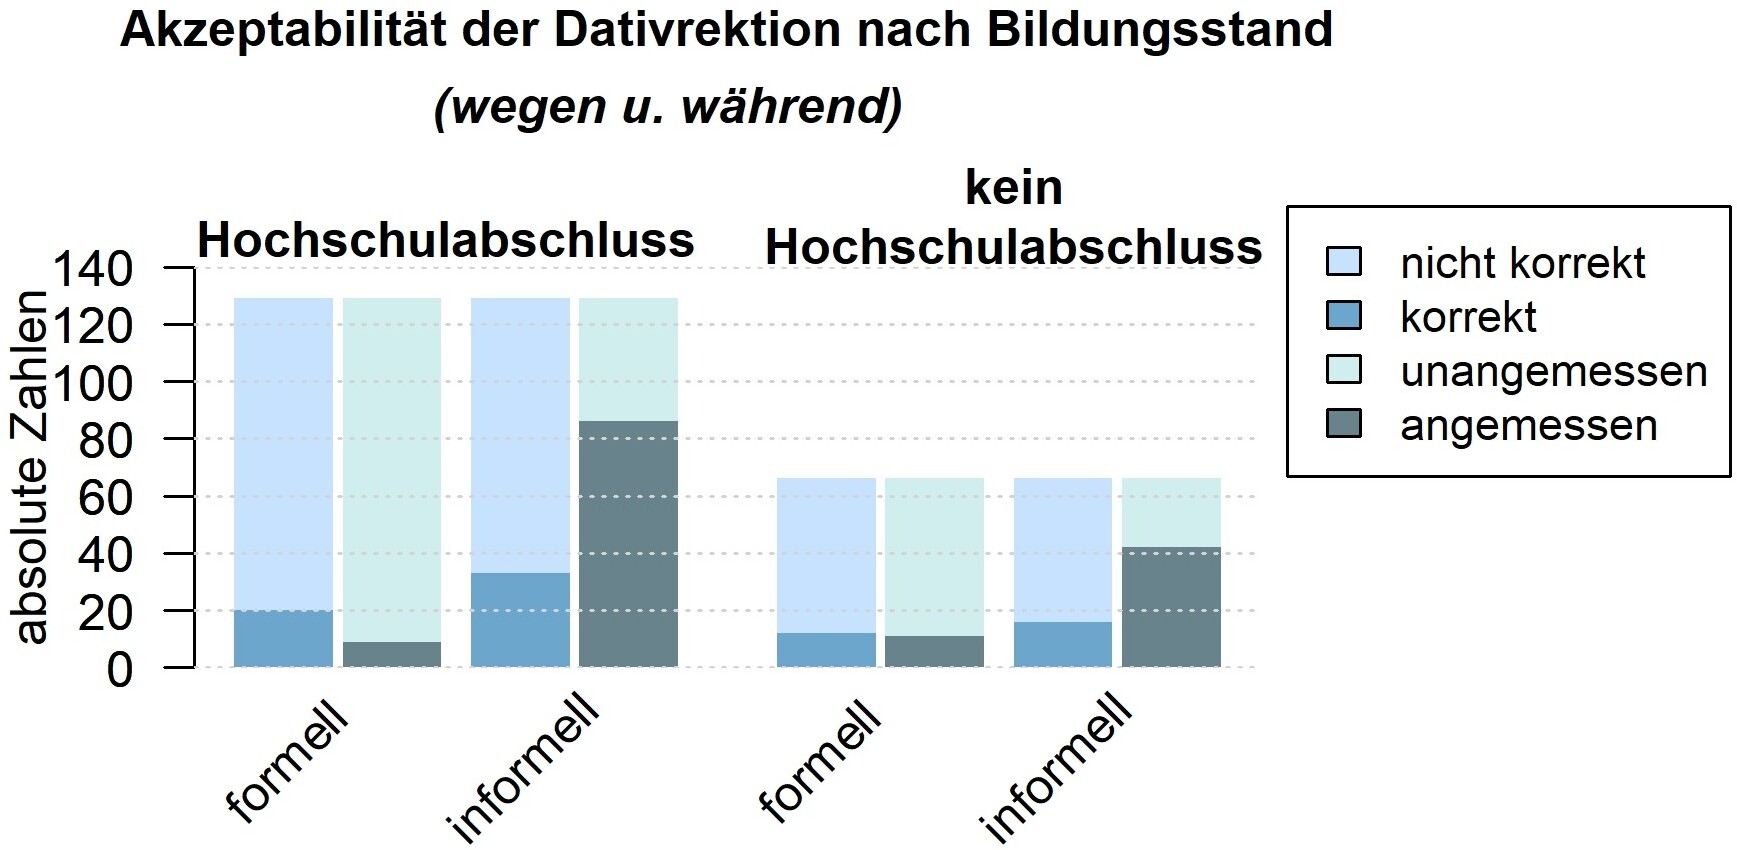
\includegraphics[scale=1]{AkzDativNachBildung.jpg}
%\caption{Akzeptabilität der Dativrektion bei \wegen{} und \waehrend{} nach Bildungsstand}
%\label{pic:AkzDativNachBildung}
%\end{figure}
%\begin{figure}
%\centering
%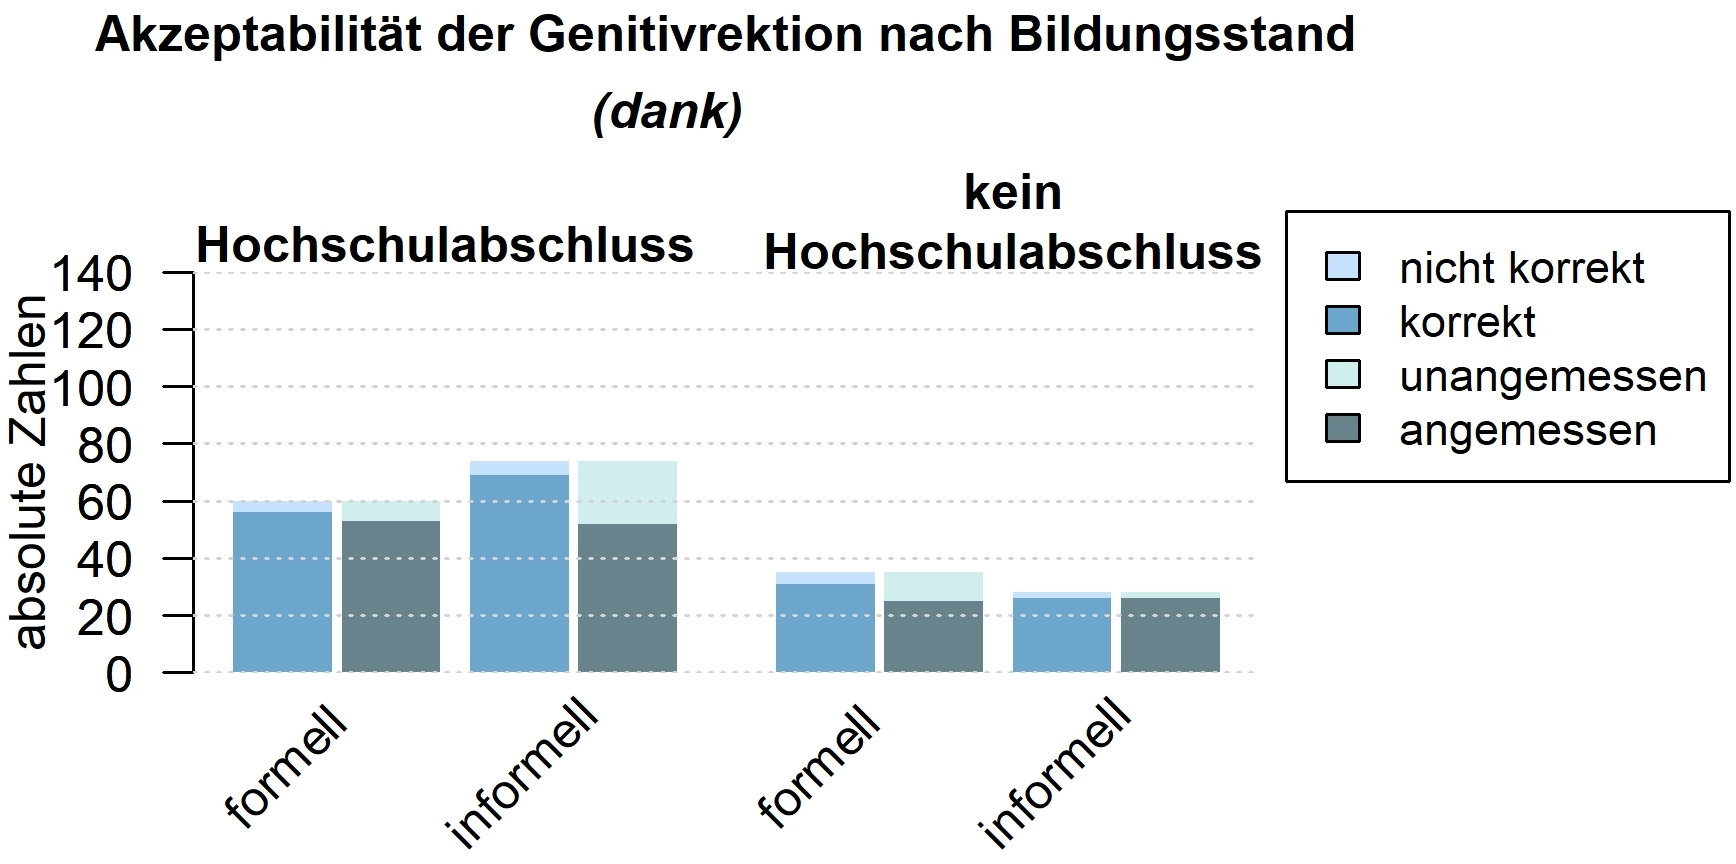
\includegraphics[scale=1]{AkzGenitivNachBildung.jpg}
%\caption{Akzeptabilität der Genitivrektion bei \dank{} nach Bildungsstand}
%\label{pic:AkzGenitivNachBildung}
%\end{figure}
\subsection{Akzeptabilität und Textaffinität des Berufs}
\label{sec:ErgAkzNachBeruf}
Teilweise werden die Varianten im Assoziationsteil nicht nur mit hoher oder niedriger Bildung, sondern auch mit hoher oder niedriger Sprachkompetenz in Verbindung gebracht (\autoref{sec:ErgAssPersonen}). 
Im Folgenden werden daher die Akzeptabilitätswerte von Befragten, die viel mit Sprache zu tun haben, mit denen von Befragten, die wenig mit Sprache zu tun haben, verglichen. 
Zwei Fragen im Fragebogen geben Aufschluss darüber, wie kompetent Personen im Bereich Sprache sind: 
Zum einen die Likertskala zur eigenen Einschätzung der Sprachsicherheit und zum anderen die Frage danach, wie häufig Befragte im Beruf mit längeren Texten zu tun haben (\autoref{sec:RE} und \autoref{sec:ME}). 
Auf der Likertskala zur Einschätzung der Sprachsicherheit erreichen 344 TeilnehmerInnen der Befragung Werte von über drei und sehen sich selbst damit als eher sicher an (\autoref{sec:Sprachsicherheit}). 
Lediglich 53 Befragte erreichen drei oder weniger Punkte auf der Likertskala, stufen ihre eigene Sprachsicherheit also niedrig ein. 
Da diese wenigen Personen im Akzeptabilitätstest auf vier Gruppen verteilt sind, ist die Aussagekraft eines Vergleichs mit der großen Anzahl derer, die sich als sprachlich sicher einstufen, wenig aussagekräftig. 
Zudem misst die Likertskala die Selbsteinschätzung der Befragten, nicht ihre tatsächliche sprachliche Sicherheit. 
Aus diesen Gründen werden für den Vergleich die Angaben zur Sprachaffinität des eigenen Berufs herangezogen (\autoref{sec:Beruf}): 
283 Befragte haben im Beruf täglich mit längeren Texten zu tun und üben damit einen textaffinen Beruf aus. 
114 Befragte haben seltener mit längeren Texten zu tun und üben damit keinen textaffinen Beruf aus. 
Zunächst werden die Ergebnisse zu \wegen{} und \waehrend{} gemeinsam betrachtet, anschließend einzeln die zu \dank{}, \gegenueber{} sowie der Primärpräposition \object{seit}. 

In den beiden Gruppen, die im Akzeptabilitätstest \wegen{} und \waehrend{} bewerten, sind insgesamt 135 Befragte mit textaffinen Berufen und 62 Befragte, deren Berufe nicht textaffin sind (s. \autoref{table:ErgAkzDativNachBeruf}). 
Aus der Gruppe mit textaffinen Berufen beurteilten 69 \wegen{} im formellen und \waehrend{} im informellen Setting und 66 \waehrend{} im formellen und \wegen{} im informellen Setting. 
Von den Befragten ohne textaffine Berufe wurden 32 nach \wegen{} im formellen und \waehrend{} im informellen Setting gefragt und 30 nach \waehrend{} im formellen und \wegen{} im informellen Setting. 
% Please add the following required packages to your document preamble:
% \usepackage{multirow}
% \usepackage[table,xcdraw]{xcolor}
% If you use beamer only pass "xcolor=table" option, i.e. \documentclass[xcolor=table]{beamer}
\begin{table}
\centering
\begin{tabular}{llrrrr}
\multicolumn{6}{l}{\wegen{} oder \waehrend{} + Dativ nach Textaffinität des Berufs}                                                                                                                                                                                                                          \\ \hline
                                                                                &                                      & \multicolumn{2}{c}{\begin{tabular}[c]{@{}c@{}}Beruf\\ textaffin\\ (n=135)\end{tabular}} & \multicolumn{2}{c}{\begin{tabular}[c]{@{}c@{}}Beruf nicht\\ textaffin\\ (n=62)\end{tabular}} \\ \hline
                                                                                & \cellcolor[HTML]{9B9B9B}korrekt      & \cellcolor[HTML]{9B9B9B}17              & \cellcolor[HTML]{9B9B9B}{\footnotesize (12,59 \%)}            & \cellcolor[HTML]{9B9B9B}15                & \cellcolor[HTML]{9B9B9B}{\footnotesize (24,19 \%)}               \\ %\cline{2-6} 
                                                                                & \cellcolor[HTML]{9B9B9B}inkorrekt    & \cellcolor[HTML]{9B9B9B}118             & \cellcolor[HTML]{9B9B9B}{\footnotesize (87,41 \%)}            & \cellcolor[HTML]{9B9B9B}47                & \cellcolor[HTML]{9B9B9B}{\footnotesize (75,81 \%)}               \\ %\cline{2-6} 
                                                                                & \cellcolor[HTML]{EFEFEF}angemessen   & \cellcolor[HTML]{EFEFEF}13              & \cellcolor[HTML]{EFEFEF}{\footnotesize (9,63 \%)}             & \cellcolor[HTML]{EFEFEF}    7              & \cellcolor[HTML]{EFEFEF}{\footnotesize (11,29 \%)}               \\ %\cline{2-6} 
                                                                                & \cellcolor[HTML]{EFEFEF}unangemessen & \cellcolor[HTML]{EFEFEF}122             & \cellcolor[HTML]{EFEFEF}{\footnotesize (90,37 \%)}            & \cellcolor[HTML]{EFEFEF}55                & \cellcolor[HTML]{EFEFEF}{\footnotesize (88,71 \%)}               \\ %\cline{2-6} 
                                                                                & eigene Verwendung ja                 & 7                                       & {\footnotesize (5,19 \%)}                                     & 9                                         & {\footnotesize (14,52 \%)}                                       \\ %\cline{2-6} 
\multirow{-6}{*}{\begin{tabular}[c]{@{}l@{}}formelles\\ Setting\end{tabular}}   & eigene Verwendung nein               & 128                                     & {\footnotesize (94,81 \%)}                                    & 53                                        & {\footnotesize (85,48 \%)}                                       \\ \hline
                                                                                &                                      & \multicolumn{2}{c}{\begin{tabular}[c]{@{}c@{}}Beruf\\ textaffin\\ (n=135)\end{tabular}} & \multicolumn{2}{c}{\begin{tabular}[c]{@{}c@{}}Beruf nicht\\ textaffin\\ (n=62)\end{tabular}} \\ \hline
                                                                                & \cellcolor[HTML]{9B9B9B}korrekt      & \cellcolor[HTML]{9B9B9B}28              & \cellcolor[HTML]{9B9B9B}{\footnotesize (20,74 \%)}            & \cellcolor[HTML]{9B9B9B}22                & \cellcolor[HTML]{9B9B9B}{\footnotesize (35,48 \%)}               \\ %\cline{2-6} 
                                                                                & \cellcolor[HTML]{9B9B9B}inkorrekt    & \cellcolor[HTML]{9B9B9B}107             & \cellcolor[HTML]{9B9B9B}{\footnotesize (79,26 \%)}            & \cellcolor[HTML]{9B9B9B}40                & \cellcolor[HTML]{9B9B9B}{\footnotesize (64,52 \%)}               \\ %\cline{2-6} 
                                                                                & \cellcolor[HTML]{EFEFEF}angemessen   & \cellcolor[HTML]{EFEFEF}89              & \cellcolor[HTML]{EFEFEF}{\footnotesize (65,93 \%)}            & \cellcolor[HTML]{EFEFEF}41                & \cellcolor[HTML]{EFEFEF}{\footnotesize (66,13 \%)}               \\ %\cline{2-6} 
                                                                                & \cellcolor[HTML]{EFEFEF}unangemessen & \cellcolor[HTML]{EFEFEF}46              & \cellcolor[HTML]{EFEFEF}{\footnotesize (34,07 \%)}            & \cellcolor[HTML]{EFEFEF}21                & \cellcolor[HTML]{EFEFEF}{\footnotesize (33,87 \%)}               \\ %\cline{2-6} 
                                                                                & eigene Verwendung ja                 & 61                                      & {\footnotesize (45,19 \%)}                                    & 35                                        & {\footnotesize (56,45 \%)}                                       \\ %\cline{2-6} 
\multirow{-6}{*}{\begin{tabular}[c]{@{}l@{}}informelles\\ Setting\end{tabular}} & eigene Verwendung nein               & 74                                      & {\footnotesize (54,81 \%)}                                    & 27                                        & {\footnotesize (43,55 \%)}                                       \\  \hline
\end{tabular}
\caption{Akzeptabilität der Dativrektion bei \wegen{} und \waehrend{} nach Textaffinität des Berufs}
\label{table:ErgAkzDativNachBeruf}
\end{table}

Befragte aus nicht-textaffinen Berufen beurteilen die Dativrektion bei \wegen{} oder \waehrend{} in beiden Settings häufiger als korrekt, die Angemessenheit schätzen sie jedoch jeweils ganz ähnlich ein wie Befragte aus textaffinen Berufen. 
Während Letztere die Dativrektion bei \wegen{} oder \waehrend{} im formellen Setting nur zu ungefähr 13~\% als korrekt erachten und zu ca. 10~\% als angemessen, empfinden in der Gruppe ohne textaffine Berufe hier rund 24~\% den Dativ als korrekt und ca. 11~\% als angemessen. 
Beide Gruppen bewerten die Varianten im informellen Setting häufiger als korrekt (ca. 21~\% aus textaffinen Berufen und 35,5~\% aus nicht-textaffinen Berufen) und als angemessen (jeweils rund 66~\%). 
Die Diskrepanz zwischen der Beurteilung der Korrektheit und der Angemessenheit ist im formellen Setting also bei Befragten aus nicht-textaffinen Berufen größer, im informellen Setting hingegen bei Befragten aus textaffinen Berufen. 
Die Frage, ob sie die Variante selbst verwenden würden, bejahen von den Befragten ohne textaffine Berufe in beiden Settings etwas mehr als von den Befragten mit textaffinen Berufen. 

Die Genitivrektion bei \dank{} wurde im formellen Setting von 68 Befragten aus textaffinen Berufen und 28 Befragten aus nicht-textaffinen Berufen beurteilt (s. \autoref{table:ErgAkzDankNachBeruf}). 
Im informellen Setting bewerteten die Variante 80 Befragte mit textaffinen Berufen und 24 Befragte ohne textaffine Berufe.
Die Prozentangaben in \autoref{table:ErgAkzDankNachBeruf} für die Gruppe ohne textaffine Berufe sind also mit Vorsicht zu betrachten. 
% Please add the following required packages to your document preamble:
% \usepackage{multirow}
% \usepackage[table,xcdraw]{xcolor}
% If you use beamer only pass "xcolor=table" option, i.e. \documentclass[xcolor=table]{beamer}
\begin{table}
\centering
\begin{tabular}{llrrrr}
\multicolumn{6}{l}{\dank{} + Genitiv nach Textaffinität des Berufs}                                                                                                                                                                                                                                      \\ \hline
                                                                                &                                      & \multicolumn{2}{c}{\begin{tabular}[c]{@{}c@{}}Beruf\\textaffin\\ (n=68)\end{tabular}} & \multicolumn{2}{c}{\begin{tabular}[c]{@{}c@{}}Beruf nicht\\textaffin\\ (n=28)\end{tabular}} \\ \hline
                                                                                & \cellcolor[HTML]{9B9B9B}korrekt      & \cellcolor[HTML]{9B9B9B}63             & \cellcolor[HTML]{9B9B9B}{\footnotesize (92,65 \%)}            & \cellcolor[HTML]{9B9B9B}24                & \cellcolor[HTML]{9B9B9B}{\footnotesize (85,71 \%)}               \\ %\cline{2-6} 
                                                                                & \cellcolor[HTML]{9B9B9B}inkorrekt    & \cellcolor[HTML]{9B9B9B}5              & \cellcolor[HTML]{9B9B9B}{\footnotesize (7,35 \%)}             & \cellcolor[HTML]{9B9B9B}4                 & \cellcolor[HTML]{9B9B9B}{\footnotesize (14,29 \%)}               \\ %\cline{2-6} 
                                                                                & \cellcolor[HTML]{EFEFEF}angemessen   & \cellcolor[HTML]{EFEFEF}57             & \cellcolor[HTML]{EFEFEF}{\footnotesize (83,82 \%)}            & \cellcolor[HTML]{EFEFEF}21                & \cellcolor[HTML]{EFEFEF}{\footnotesize (75 \%)}                  \\ %\cline{2-6} 
                                                                                & \cellcolor[HTML]{EFEFEF}unangemessen & \cellcolor[HTML]{EFEFEF}11             & \cellcolor[HTML]{EFEFEF}{\footnotesize (16,18 \%)}            & \cellcolor[HTML]{EFEFEF}7                 & \cellcolor[HTML]{EFEFEF}{\footnotesize (25 \%)}                  \\ %\cline{2-6} 
                                                                                & eigene Verwendung ja                 & 49                                     & {\footnotesize (72,06 \%)}                                    & 19                                        & {\footnotesize (67,86 \%)}                                       \\ %\cline{2-6} 
\multirow{-6}{*}{\begin{tabular}[c]{@{}l@{}}formelles\\ Setting\end{tabular}}   & eigene Verwendung nein               & 19                                     & {\footnotesize (27,94 \%)}                                    & 9                                         & {\footnotesize (32,14 \%)}                                       \\ \hline
                                                                                &                                      & \multicolumn{2}{c}{\begin{tabular}[c]{@{}c@{}}Beruf\\textaffin\\ (n=80)\end{tabular}} & \multicolumn{2}{c}{\begin{tabular}[c]{@{}c@{}}Beruf nicht\\textaffin\\ (n=24)\end{tabular}} \\ \hline
                                                                                & \cellcolor[HTML]{9B9B9B}korrekt      & \cellcolor[HTML]{9B9B9B}75             & \cellcolor[HTML]{9B9B9B}{\footnotesize (93,75 \%)}            & \cellcolor[HTML]{9B9B9B}22                & \cellcolor[HTML]{9B9B9B}{\footnotesize (91,67 \%)}               \\ %\cline{2-6} 
                                                                                & \cellcolor[HTML]{9B9B9B}inkorrekt    & \cellcolor[HTML]{9B9B9B}5              & \cellcolor[HTML]{9B9B9B}{\footnotesize (6,25 \%)}             & \cellcolor[HTML]{9B9B9B}2                 & \cellcolor[HTML]{9B9B9B}{\footnotesize (8,33 \%)}                \\ %\cline{2-6} 
                                                                                & \cellcolor[HTML]{EFEFEF}angemessen   & \cellcolor[HTML]{EFEFEF}60             & \cellcolor[HTML]{EFEFEF}{\footnotesize (75 \%)}               & \cellcolor[HTML]{EFEFEF}20                & \cellcolor[HTML]{EFEFEF}{\footnotesize (83,33 \%)}               \\ %\cline{2-6} 
                                                                                & \cellcolor[HTML]{EFEFEF}unangemessen & \cellcolor[HTML]{EFEFEF}20             & \cellcolor[HTML]{EFEFEF}{\footnotesize (25 \%)}               & \cellcolor[HTML]{EFEFEF}4                 & \cellcolor[HTML]{EFEFEF}{\footnotesize (16,67 \%)}               \\ %\cline{2-6} 
                                                                                & eigene Verwendung ja                 & 60                                     & {\footnotesize (75 \%)}                                       & 16                                        & {\footnotesize (66,67 \%)}                                       \\ %\cline{2-6} 
\multirow{-6}{*}{\begin{tabular}[c]{@{}l@{}}informelles\\ Setting\end{tabular}} & eigene Verwendung nein               & 20                                     & {\footnotesize (25 \%)}                                       & 8                                         & {\footnotesize (33,33 \%)}                                       \\ \hline 
\end{tabular}
\caption{Akzeptabilität der Genitivrektion bei \dank{} nach Textaffinität des Berufs}
\label{table:ErgAkzDankNachBeruf}
\end{table}
 In beiden Settings zeigen sich zwischen den beiden Gruppen nur geringe Unterschiede in den Angaben zu Korrektheit, Angemessenheit und eigener Verwendung, die sich aufgrund der geringen Zahl Befragter ohne textaffine Berufe kaum interpretieren lassen.

Da die gleichen Gruppen von Befragten, die im Akzeptabilitätstest vom Zufallsmechanismus für \dank{} eingeteilt wurden, \gegenueber{} mit dem Genitiv im jeweils anderen Setting bewerteten, sind auch hier die Stichproben für Befragte ohne textaffine Berufe klein (s. \autoref{table:ErgAkzGegenueberNachBeruf}). 
Im formellen Setting sind die Unterschiede zwischen Befragten mit und ohne textaffine Berufe etwas größer als bei \dank:
Von den 80 Befragten aus textaffinen Berufen bewertet jeweils ungefähr ein Drittel \gegenueber{} plus Genitiv als korrekt und angemessen. 
Unter den 24 Befragten aus nicht-textaffinen Berufen sieht jeweils ungefähr die Hälfte die Variante als korrekt und angemessen an. 
Aufgrund der geringen Stichprobe kann es sich allerdings um zufällige Unterschiede handeln. 
% Please add the following required packages to your document preamble:
% \usepackage{multirow}
% \usepackage[table,xcdraw]{xcolor}
% If you use beamer only pass "xcolor=table" option, i.e. \documentclass[xcolor=table]{beamer}
\begin{table}
\centering
\begin{tabular}{llrrrr}
\multicolumn{6}{l}{\gegenueber{} + Genitiv nach Textaffinität des Berufs}                                                                                                                                                                                                                                \\ \hline
                                                                                &                                      & \multicolumn{2}{c}{\begin{tabular}[c]{@{}c@{}}Beruf\\ textaffin\\ (n=80)\end{tabular}} & \multicolumn{2}{c}{\begin{tabular}[c]{@{}c@{}}Beruf nicht\\ textaffin\\ (n=24)\end{tabular}} \\ \hline
                                                                                & \cellcolor[HTML]{9B9B9B}korrekt      & \cellcolor[HTML]{9B9B9B}27             & \cellcolor[HTML]{9B9B9B}{\footnotesize (33,75 \%)}            & \cellcolor[HTML]{9B9B9B}13                & \cellcolor[HTML]{9B9B9B}{\footnotesize (54,17 \%)}               \\ %\cline{2-6} 
                                                                                & \cellcolor[HTML]{9B9B9B}inkorrekt    & \cellcolor[HTML]{9B9B9B}53             & \cellcolor[HTML]{9B9B9B}{\footnotesize (66,25 \%)}            & \cellcolor[HTML]{9B9B9B}11                & \cellcolor[HTML]{9B9B9B}{\footnotesize (45,83 \%)}               \\ %\cline{2-6} 
                                                                                & \cellcolor[HTML]{EFEFEF}angemessen   & \cellcolor[HTML]{EFEFEF}29             & \cellcolor[HTML]{EFEFEF}{\footnotesize (36,25 \%)}            & \cellcolor[HTML]{EFEFEF}12                & \cellcolor[HTML]{EFEFEF}{\footnotesize (50 \%)}                  \\ %\cline{2-6} 
                                                                                & \cellcolor[HTML]{EFEFEF}unangemessen & \cellcolor[HTML]{EFEFEF}51             & \cellcolor[HTML]{EFEFEF}{\footnotesize (63,75 \%)}            & \cellcolor[HTML]{EFEFEF}12                & \cellcolor[HTML]{EFEFEF}{\footnotesize (50 \%)}                  \\ %\cline{2-6} 
                                                                                & eigene Verwendung ja                 & 22                                     & {\footnotesize (27,5 \%)}                                     & 11                                        & {\footnotesize (45,83 \%)}                                       \\ %\cline{2-6} 
\multirow{-6}{*}{\begin{tabular}[c]{@{}l@{}}formelles\\ Setting\end{tabular}}   & eigene Verwendung nein               & 58                                     & {\footnotesize (72,5 \%)}                                     & 13                                        & {\footnotesize (54,17 \%)}                                       \\ \hline
                                                                                &                                      & \multicolumn{2}{c}{\begin{tabular}[c]{@{}c@{}}Beruf\\ textaffin\\ (n=68)\end{tabular}} & \multicolumn{2}{c}{\begin{tabular}[c]{@{}c@{}}Beruf nicht\\ textaffin\\ (n=28)\end{tabular}} \\ \hline
                                                                                & \cellcolor[HTML]{9B9B9B}korrekt      & \cellcolor[HTML]{9B9B9B}21             & \cellcolor[HTML]{9B9B9B}{\footnotesize (30,88 \%)}            & \cellcolor[HTML]{9B9B9B}10                & \cellcolor[HTML]{9B9B9B}{\footnotesize (35,71 \%)}               \\ %\cline{2-6} 
                                                                                & \cellcolor[HTML]{9B9B9B}inkorrekt    & \cellcolor[HTML]{9B9B9B}47             & \cellcolor[HTML]{9B9B9B}{\footnotesize (69,12 \%)}            & \cellcolor[HTML]{9B9B9B}18                & \cellcolor[HTML]{9B9B9B}{\footnotesize (64,29 \%)}               \\ %\cline{2-6} 
                                                                                & \cellcolor[HTML]{EFEFEF}angemessen   & \cellcolor[HTML]{EFEFEF}26             & \cellcolor[HTML]{EFEFEF}{\footnotesize (38,24 \%)}            & \cellcolor[HTML]{EFEFEF}10                & \cellcolor[HTML]{EFEFEF}{\footnotesize (35,71 \%)}               \\ %\cline{2-6} 
                                                                                & \cellcolor[HTML]{EFEFEF}unangemessen & \cellcolor[HTML]{EFEFEF}42             & \cellcolor[HTML]{EFEFEF}{\footnotesize (61,76 \%)}            & \cellcolor[HTML]{EFEFEF}18                & \cellcolor[HTML]{EFEFEF}{\footnotesize (64,29 \%)}               \\ %\cline{2-6} 
                                                                                & eigene Verwendung ja                 & 17                                     & {\footnotesize (25 \%)}                                       & 4                                         & {\footnotesize (14,29 \%)}                                       \\ %\cline{2-6} 
\multirow{-6}{*}{\begin{tabular}[c]{@{}l@{}}informelles\\ Setting\end{tabular}} & eigene Verwendung nein               & 51                                     & {\footnotesize (75 \%)}                                       & 24                                        & {\footnotesize (85,71 \%)}                                       \\  \hline
\end{tabular}
\caption{Akzeptabilität der Genitivrektion bei \gegenueber{} nach Textaffinität des Berufs}
\label{table:ErgAkzGegenueberNachBeruf}
\end{table}

Die Ergebnisse zur Primärpräposition \object{seit} mit dem Genitiv lassen sich besser vergleichen, da diese Form von allen Befragten im Akzeptabilitätstest bewertet wurde (s. \autoref{table:ErgAkzSeitNachBeruf}). 
Es zeigt sich, dass Befragte aus textaffinen Berufen \object{seit} plus Genitiv durchweg negativer bewerten als Befragte aus nicht-textaffinen Berufen. 
Im formellen Setting beurteilen Erstere die Form zu rund 27~\% als korrekt und zu ca. 28~\% als angemessen. 
Ungefähr 23~\% geben an, die Genitivrektion bei \object{seit} in einem förmlichen Brief an ein Amt selbst zu verwenden. 
Unter den Befragten ohne textaffine Berufe empfinden jeweils rund 45~\% die abgefragte Form im formellen Setting als korrekt und angemessen, ca. 40~\% geben an, sie selbst zu verwenden. 
Unter den Befragten mit textaffinen Berufen beurteilen im informellen Setting nur jeweils etwas weniger \object{seit} plus Genitiv als korrekt und angemessen. 
Befragte aus nicht-textaffinen Berufen hingegen bewerten Korrekhteit und Angemessenheit bei \object{seit} stärker kontextabhängig. 
Zwar ist der Anteil derer, die angeben, die Form sei korrekt und angemessen und würde von ihnen verwendet, unter den Befragten aus nicht-textaffinen Berufen im informellen Setting immer noch größer. 
Die Differenzen zwischen den Gruppen sind hier aber kleiner.
% Please add the following required packages to your document preamble:
% \usepackage{multirow}
% \usepackage[table,xcdraw]{xcolor}
% If you use beamer only pass "xcolor=table" option, i.e. \documentclass[xcolor=table]{beamer}
\begin{table}
\centering
\begin{tabular}{llrrrr}
\multicolumn{6}{l}{\object{seit} + Genitiv nach Textaffinität des Berufs}                                                                                                                                                                                                                                        \\ \hline
                                                                                &                                      & \multicolumn{2}{c}{\begin{tabular}[c]{@{}c@{}}Beruf\\ textaffin\\ (n=283)\end{tabular}} & \multicolumn{2}{c}{\begin{tabular}[c]{@{}c@{}}Beruf nicht\\ textaffin\\ (n=114)\end{tabular}} \\ \hline
                                                                                & \cellcolor[HTML]{9B9B9B}korrekt      & \cellcolor[HTML]{9B9B9B}76              & \cellcolor[HTML]{9B9B9B}{\footnotesize (26,86 \%)}            & \cellcolor[HTML]{9B9B9B}51                & \cellcolor[HTML]{9B9B9B}{\footnotesize (44,74 \%)}                \\ %\cline{2-6} 
                                                                                & \cellcolor[HTML]{9B9B9B}inkorrekt    & \cellcolor[HTML]{9B9B9B}207             & \cellcolor[HTML]{9B9B9B}{\footnotesize (73,14 \%)}            & \cellcolor[HTML]{9B9B9B}63                & \cellcolor[HTML]{9B9B9B}{\footnotesize (55,26 \%)}                \\ %\cline{2-6} 
                                                                                & \cellcolor[HTML]{EFEFEF}angemessen   & \cellcolor[HTML]{EFEFEF}80              & \cellcolor[HTML]{EFEFEF}{\footnotesize (28,27 \%)}            & \cellcolor[HTML]{EFEFEF}51                & \cellcolor[HTML]{EFEFEF}{\footnotesize (44,74 \%)}                \\ %\cline{2-6} 
                                                                                & \cellcolor[HTML]{EFEFEF}unangemessen & \cellcolor[HTML]{EFEFEF}203             & \cellcolor[HTML]{EFEFEF}{\footnotesize (71,73 \%)}            & \cellcolor[HTML]{EFEFEF}63                & \cellcolor[HTML]{EFEFEF}{\footnotesize (55,26 \%)}                \\ %\cline{2-6} 
                                                                                & eigene Verwendung ja                 & 65                                      & {\footnotesize (22,97 \%)}                                    & 45                                        & {\footnotesize (39,47 \%)} \\ %\cline{2-6} 
\multirow{-6}{*}{\begin{tabular}[c]{@{}l@{}}formelles\\ Setting\end{tabular}}   & eigene Verwendung nein               & 218                                     & {\footnotesize (77,03 \%)}                                    & 69                                        & {\footnotesize (60,53 \%)}   \\ \hline
                                                                                &                                      & \multicolumn{2}{c}{\begin{tabular}[c]{@{}c@{}}Beruf\\ textaffin\\ (n=283)\end{tabular}} & \multicolumn{2}{c}{\begin{tabular}[c]{@{}c@{}}Beruf nicht\\ textaffin\\ (n=114)\end{tabular}} \\ \hline
                                                                                & \cellcolor[HTML]{9B9B9B}korrekt      & \cellcolor[HTML]{9B9B9B}50              & \cellcolor[HTML]{9B9B9B}{\footnotesize (17,67 \%)}            & \cellcolor[HTML]{9B9B9B}36                & \cellcolor[HTML]{9B9B9B}{\footnotesize (31,58 \%)}                \\ %\cline{2-6} 
                                                                                & \cellcolor[HTML]{9B9B9B}inkorrekt    & \cellcolor[HTML]{9B9B9B}233             & \cellcolor[HTML]{9B9B9B}{\footnotesize (82,33 \%)}            & \cellcolor[HTML]{9B9B9B}78                & \cellcolor[HTML]{9B9B9B}{\footnotesize (68,42 \%)}                \\ %\cline{2-6} 
                                                                                & \cellcolor[HTML]{EFEFEF}angemessen   & \cellcolor[HTML]{EFEFEF}60              & \cellcolor[HTML]{EFEFEF}{\footnotesize (21,2 \%)}             & \cellcolor[HTML]{EFEFEF}34                & \cellcolor[HTML]{EFEFEF}{\footnotesize (29,82 \%)}                \\ %\cline{2-6} 
                                                                                & \cellcolor[HTML]{EFEFEF}unangemessen & \cellcolor[HTML]{EFEFEF}223             & \cellcolor[HTML]{EFEFEF}{\footnotesize (78,8 \%)}             & \cellcolor[HTML]{EFEFEF}80                & \cellcolor[HTML]{EFEFEF}{\footnotesize (70,18 \%)}                \\ %\cline{2-6} 
                                                                                & eigene Verwendung ja                 & 27                                      & {\footnotesize (9,54 \%)}                                     & 24                                        & {\footnotesize (21,05 \%)}                                        \\ %\cline{2-6} 
\multirow{-6}{*}{\begin{tabular}[c]{@{}l@{}}informelles\\ Setting\end{tabular}} & eigene Verwendung nein               & 256                                     & {\footnotesize (90,46 \%)}                                    & 90                                        & {\footnotesize (78,95 \%)}                                        \\ \hline
\end{tabular}
\caption{Akzeptabilität der Genitivrektion bei \object{seit} nach Textaffinität des Berufs}
\label{table:ErgAkzSeitNachBeruf}
\end{table}

Der Vergleich der Akzeptabilitätsangaben von Befragten, die im Beruf häufig oder täglich mit längeren Texten zu tun haben, und Befragten, die im Beruf seltener mit längeren Texten zu tun haben, ergibt zusammengefassst folgende Ergebnisse:
Die Dativrektion bei \wegen{} und \waehrend{} wird von Befragten aus textaffinen Berufen in beiden Settings etwas seltener als korrekt bewertet. 
Sie geben auch seltener an, diese Formen selbst zu verwenden. 
Die Angemessenheit wird jedoch in beiden Gruppen ähnlich beurteilt. 
Bei \dank{} und \gegenueber{} mit der Genitivrektion zeigen sich nur geringe Unterschiede, die sich aufgrund der kleinen Stichproben nicht deuten lassen. 
Die Primärpräposition \object{seit} mit der Genitivrektion wird von Befragten aus textaffinen Berufen in beiden Settings seltener als korrekt und angemessen bewertet. 
Die Frage nach der eigenen Verwendung bejahen hier unter den Befragten aus textaffinen Berufen ebenfalls weniger. 
\subsection{Akzeptabilität und Variationstoleranz}
\label{sec:ErgAkzNachVT}
% Akzeptabilität nach Variationstoleranz
Wie in \autoref{sec:Variationstoleranz} dargestellt, unterscheiden sich die Befragten in ihrer Toleranz gegenüber sprachlicher Variation. 
Sie lassen sich in eher variationstolerante und eher wenig variationstolerante Personen unterteilen. 
Hierfür werden ihre Antworten auf der Likertskala zur Variationstoleranz am Beginn des Fragebogens herangezogen: 
Personen, die auf der Likertskala zur Variationstoleranz Werte zwischen null und drei erreichen, bilden die wenig variationstolerante Gruppe (abgekürzt als Vt--), während Personen, die Werte von über drei erreichen, als variationstolerant gelten können (abgekürzt als Vt+). 
Ob Befragte, die Variation gegenüber generell offener sind, sich im Akzeptabilitätstest anders verhalten als Befragte, die Variation ablehnen, ist Thema dieses Abschnitts. 
Wieder werden erst die summierten Akzeptabilitätswerte zu \wegen{} und \waehrend{}, dann einzeln die zu \dank{}, \gegenueber{} und der Primärpräposition \object{seit} betrachtet. 

Von den Befragten, die im Akzeptabilitätstest in einer der beiden Gruppen mit den ursprünglichen Genitivpräpositionen \wegen{} und \waehrend{} waren, können 108 aufgrund ihrer Antworten auf der Likertskala als variationstolerant (Vt+) eingestuft werden (s. \autoref{table:ErgAkzDativNachVT}).
Davon bewertete genau die Hälfte (54) \wegen{} im formellen und \waehrend{} im informellen Kontext, bei der anderen Hälfte wurden die Präpositionen im jeweils anderen Kontext abgefragt. 
89 Befragte, die im Akzeptabilitätstest \wegen{} oder \waehrend{} beurteilten, können als weniger variationstolerant (Vt--) klassifiziert werden.
47 von ihnen wurden im formellen Setting nach der Akzeptabilität von \wegen{} plus Dativ gefragt und im informellen Setting nach der Akzeptabilität von \waehrend{} plus Dativ. 
Bei 42 Befragten der Gruppe Vt-- war die Verteilung der Präpositionen auf die Settings umgekehrt. 
% Please add the following required packages to your document preamble:
% \usepackage{multirow}
% \usepackage[table,xcdraw]{xcolor}
% If you use beamer only pass "xcolor=table" option, i.e. \documentclass[xcolor=table]{beamer}
\begin{table}
\centering
\begin{tabular}{llrrrr}
\multicolumn{6}{l}{\wegen{} oder \waehrend{} + Dativ nach Variationstoleranz}                                                                                                                                                                                               \\ \hline
                                                                                &                                      & \multicolumn{2}{c}{\begin{tabular}[c]{@{}c@{}}Vt+\\ (n=108)\end{tabular}} & \multicolumn{2}{c}{\begin{tabular}[c]{@{}c@{}}Vt--\\ (n=89)\end{tabular}} \\ \hline
                                                                                & \cellcolor[HTML]{9B9B9B}korrekt      & \cellcolor[HTML]{9B9B9B}19      & \cellcolor[HTML]{9B9B9B}{\footnotesize (17,59 \%)}       & \cellcolor[HTML]{9B9B9B}13      & \cellcolor[HTML]{9B9B9B}{\footnotesize (14,61 \%)}      \\ %\cline{2-6} 
                                                                                & \cellcolor[HTML]{9B9B9B}inkorrekt    & \cellcolor[HTML]{9B9B9B}89      & \cellcolor[HTML]{9B9B9B}{\footnotesize (82,41 \%)}      & \cellcolor[HTML]{9B9B9B}76      & \cellcolor[HTML]{9B9B9B}{\footnotesize (85,39 \%)}      \\ %\cline{2-6} 
                                                                                & \cellcolor[HTML]{EFEFEF}angemessen   & \cellcolor[HTML]{EFEFEF}12      & \cellcolor[HTML]{EFEFEF}{\footnotesize (11,11 \%)}      & \cellcolor[HTML]{EFEFEF}8       & \cellcolor[HTML]{EFEFEF}{\footnotesize (8,99 \%)}       \\ %\cline{2-6} 
                                                                                & \cellcolor[HTML]{EFEFEF}unangemessen & \cellcolor[HTML]{EFEFEF}96      & \cellcolor[HTML]{EFEFEF}{\footnotesize (88,89 \%)}      & \cellcolor[HTML]{EFEFEF}81      & \cellcolor[HTML]{EFEFEF}{\footnotesize (91,01 \%)}      \\ %\cline{2-6} 
                                                                                & eigene Verwendung ja                 & 12                              & {\footnotesize (11,11 \%)}                              & 4                               & {\footnotesize (4,49 \%)}                               \\ %\cline{2-6} 
\multirow{-6}{*}{\begin{tabular}[c]{@{}l@{}}formelles\\ Setting\end{tabular}}   & eigene Verwendung nein               & 96                              & {\footnotesize (88,89 \%)}                              & 85                              & {\footnotesize (95,51 \%)}                              \\ \hline
                                                                                &                                      & \multicolumn{2}{c}{\begin{tabular}[c]{@{}c@{}}Vt+\\ (n=108)\end{tabular}} & \multicolumn{2}{c}{\begin{tabular}[c]{@{}c@{}}Vt--\\ (n=89)\end{tabular}} \\ \hline
                                                                                & \cellcolor[HTML]{9B9B9B}korrekt      & \cellcolor[HTML]{9B9B9B}36      & \cellcolor[HTML]{9B9B9B}{\footnotesize (33,33 \%)}      & \cellcolor[HTML]{9B9B9B}14      & \cellcolor[HTML]{9B9B9B}{\footnotesize (15,73 \%)}      \\ %\cline{2-6} 
                                                                                & \cellcolor[HTML]{9B9B9B}inkorrekt    & \cellcolor[HTML]{9B9B9B}72      & \cellcolor[HTML]{9B9B9B}{\footnotesize (66,67 \%)}      & \cellcolor[HTML]{9B9B9B}75      & \cellcolor[HTML]{9B9B9B}{\footnotesize (84,27 \%)}      \\ %\cline{2-6} 
                                                                                & \cellcolor[HTML]{EFEFEF}angemessen   & \cellcolor[HTML]{EFEFEF}79      & \cellcolor[HTML]{EFEFEF}{\footnotesize (73,15 \%)}      & \cellcolor[HTML]{EFEFEF}51      & \cellcolor[HTML]{EFEFEF}{\footnotesize (57,3 \%)}       \\ %\cline{2-6} 
                                                                                & \cellcolor[HTML]{EFEFEF}unangemessen & \cellcolor[HTML]{EFEFEF}29      & \cellcolor[HTML]{EFEFEF}{\footnotesize (26,85 \%)}      & \cellcolor[HTML]{EFEFEF}38      & \cellcolor[HTML]{EFEFEF}{\footnotesize (42,7 \%)}       \\ %\cline{2-6} 
                                                                                & eigene Verwendung ja                 & 64                              & {\footnotesize (59,26 \%)}                              & 32                              & {\footnotesize (35,96 \%)}                              \\ %\cline{2-6} 
\multirow{-6}{*}{\begin{tabular}[c]{@{}l@{}}informelles\\ Setting\end{tabular}} & eigene Verwendung nein               & 44                              & {\footnotesize (40,74 \%)}                              & 57                              & {\footnotesize (64,04 \%)}                              \\ \hline
\end{tabular}
\caption{Akzeptabilität der Dativrektion bei \wegen{} und \waehrend{} nach Variationstoleranz}
\label{table:ErgAkzDativNachVT}
\end{table}

Ein interessantes Ergebnis des Vergleichs der Gruppe Vt+ mit der Gruppe Vt-- ist, dass sich die Gruppen offenbar in ihrer Beurteilung der Korrektheit der Dativrektion unterscheiden: 
Diese wird von den Befragten, die Variation eher ablehnen, unabhängig vom Kontext bewertet.
In einem Brief an ein Amt empfinden 76 von 89 wenig variationstoleranten Befragten die Dativrektion als inkorrekt, in einem Gespräch mit einem Freund 75. 
Befragte der Gruppe Vt+ hingegen ordnen die Dativrektion im informellen Setting deutlich häufiger (36-mal) als korrekt ein als im formellen Setting (19-mal). 
Die Angemessenheit der Varianten wird von allen Befragten unabhängig von ihrer Variationstoleranz in Abhängigkeit vom Kontext beurteilt.
Der Anteil derer, die den Dativ im informellen Kontext als angemessen ansehen, ist unter den variationstoleranten Befragten jedoch höher als unter den nicht variationstoleranten (79 von 108 im Vergleich zu 51 von 89). 

Im informellen Setting zeigen sich zudem große Unterschiede bei den Angaben zur eigenen Verwendung. 
Eine Mehrheit der variationstoleranten Befragten würde die Dativrektion bei \wegen{} oder \waehrend{} verwenden (64 von 108), von den nicht variationstoleranten Befragten gibt dies jedoch nur ca. ein Drittel an (32 von 89). 

Die beiden Gruppen, die aufgrund des Zufallsmechanismus im Akzeptabilitätstest die Genitivrektion bei ursprünglichen Dativpräpositionen beurteilten, teilen sich wie folgt auf: 
59 Befragte der Gruppe Vt+ und 37 Befragte der Gruppe Vt-- bewerteten \dank{} im formellen und \gegenueber{} im informellen Setting (s. \autoref{table:ErgAkzDankNachVT} und \autoref{table:ErgAkzGegenueberNachVT}). 
61 Befragte der Gruppe Vt+ und 43 Befragte der Gruppe Vt-- beurteilten umgekehrt \gegenueber{} im formellen und \dank{} im informellen Setting. 

Bei \dank{} plus Genitiv zeigen sich wenig nennenswerte Unterschiede zwischen den Gruppen.
Die Variante wird mehrheitlich akzeptiert. 
Im formellen Kontext wird die Genitivrektion bei \dank{} von Befragten der Gruppe Vt-- allerdings eher abgelehnt als von Befragten der Gruppe Vt+: 
Ungefähr ein Drittel der Befragten mit Vt-- empfindet \dank{} plus Genitiv in einem Brief an ein Amt als unangemessen. 
Unter den Befragten mit Vt+ ist der Anteil kleiner (sieben von 59). 
% Please add the following required packages to your document preamble:
% \usepackage{multirow}
% \usepackage[table,xcdraw]{xcolor}
% If you use beamer only pass "xcolor=table" option, i.e. \documentclass[xcolor=table]{beamer}
\begin{table}
\centering
\begin{tabular}{llrrrr}
\multicolumn{6}{l}{\dank{} + Genitiv nach Variationstoleranz}                                                                                                                                                                                                           \\ \hline
                                                                                &                                      & \multicolumn{2}{c}{\begin{tabular}[c]{@{}c@{}}Vt+\\ (n=59)\end{tabular}} & \multicolumn{2}{c}{\begin{tabular}[c]{@{}c@{}}Vt--\\ (n=37)\end{tabular}} \\ \hline
                                                                                & \cellcolor[HTML]{9B9B9B}korrekt      & \cellcolor[HTML]{9B9B9B}55      & \cellcolor[HTML]{9B9B9B}{\footnotesize (93,22 \%)}     & \cellcolor[HTML]{9B9B9B}32      & \cellcolor[HTML]{9B9B9B}{\footnotesize (86,49 \%)}      \\ %\cline{2-6} 
                                                                                & \cellcolor[HTML]{9B9B9B}inkorrekt    & \cellcolor[HTML]{9B9B9B}4       & \cellcolor[HTML]{9B9B9B}{\footnotesize (6,78 \%)}      & \cellcolor[HTML]{9B9B9B}5       & \cellcolor[HTML]{9B9B9B}{\footnotesize (13,51 \%)}      \\ %\cline{2-6} 
                                                                                & \cellcolor[HTML]{EFEFEF}angemessen   & \cellcolor[HTML]{EFEFEF}52      & \cellcolor[HTML]{EFEFEF}{\footnotesize (88,14 \%)}     & \cellcolor[HTML]{EFEFEF}26      & \cellcolor[HTML]{EFEFEF}{\footnotesize (70,27 \%)}      \\ %\cline{2-6} 
                                                                                & \cellcolor[HTML]{EFEFEF}unangemessen & \cellcolor[HTML]{EFEFEF}7       & \cellcolor[HTML]{EFEFEF}{\footnotesize (11,86 \%})     & \cellcolor[HTML]{EFEFEF}11      & \cellcolor[HTML]{EFEFEF}{\footnotesize (29,73 \%)}      \\ %\cline{2-6} 
                                                                                & eigene Verwendung ja                 & 47                              & {\footnotesize (79,66 \%)}                             & 21                              & {\footnotesize (56,76 \%)}                              \\ \cline{2-6} 
\multirow{-6}{*}{\begin{tabular}[c]{@{}l@{}}formelles\\ Setting\end{tabular}}   & eigene Verwendung nein               & 12                              & {\footnotesize (20,34 \%)}                             & 16                              & {\footnotesize (43,24 \%)}                              \\ \hline
                                                                                &                                      & \multicolumn{2}{c}{\begin{tabular}[c]{@{}c@{}}Vt+\\ (n=61)\end{tabular}} & \multicolumn{2}{c}{\begin{tabular}[c]{@{}c@{}}Vt--\\ (n=43)\end{tabular}} \\ \hline
                                                                                & \cellcolor[HTML]{9B9B9B}korrekt      & \cellcolor[HTML]{9B9B9B}57      & \cellcolor[HTML]{9B9B9B}{\footnotesize (93,44 \%)}     & \cellcolor[HTML]{9B9B9B}40      & \cellcolor[HTML]{9B9B9B}{\footnotesize (93,02 \%)}      \\ %\cline{2-6} 
                                                                                & \cellcolor[HTML]{9B9B9B}inkorrekt    & \cellcolor[HTML]{9B9B9B}4       & \cellcolor[HTML]{9B9B9B}{\footnotesize (6,56 \%)}      & \cellcolor[HTML]{9B9B9B}3       & \cellcolor[HTML]{9B9B9B}{\footnotesize (6,98 \%)}       \\ %\cline{2-6} 
                                                                                & \cellcolor[HTML]{EFEFEF}angemessen   & \cellcolor[HTML]{EFEFEF}46      & \cellcolor[HTML]{EFEFEF}{\footnotesize (75,41 \%)}     & \cellcolor[HTML]{EFEFEF}34      & \cellcolor[HTML]{EFEFEF}{\footnotesize (79,07 \%)}      \\ %\cline{2-6} 
                                                                                & \cellcolor[HTML]{EFEFEF}unangemessen & \cellcolor[HTML]{EFEFEF}15      & \cellcolor[HTML]{EFEFEF}{\footnotesize (24,59 \%)}     & \cellcolor[HTML]{EFEFEF}9       & \cellcolor[HTML]{EFEFEF}{\footnotesize (20,93 \%)}      \\ %\cline{2-6} 
                                                                                & eigene Verwendung ja                 & 44                              & {\footnotesize (72,13 \%)}                             & 32                              & {\footnotesize (74,42 \%)}                              \\ %\cline{2-6} 
\multirow{-6}{*}{\begin{tabular}[c]{@{}l@{}}informelles\\ Setting\end{tabular}} & eigene Verwendung nein               & 17                              & {\footnotesize (27,87 \%)}                             & 11                              & {\footnotesize (25,58 \%)}                              \\ \hline
\end{tabular}
\caption{Akzeptabilität der Genitivrektion bei \dank{} nach Variationstoleranz}
\label{table:ErgAkzDankNachVT}
\end{table}

\object{Gegenüber} mit dem Genitiv wird von beiden Gruppen gleichermaßen mehrheitlich abgelehnt. 
Im formellen Setting beurteilen Befragte der Gruppe Vt-- die Variante etwas häufiger als korrekt und angemessen. 
Im informellen Setting zeigt sich folgender Unterschied: 
Aus der variationstoleranteren Gruppe finden \gegenueber{} plus Genitiv  etwas mehr Befragte in einem Gespräch mit einem Freund angemessen als korrekt. 
Dies ist in der Gruppe der Befragten mit geringerer Toleranz für Variation nicht der Fall. 
Aufgrund der kleinen Stichprobe kann es sich aber um eine zufällige Verteilung handeln. 
% Please add the following required packages to your document preamble:
% \usepackage{multirow}
% \usepackage[table,xcdraw]{xcolor}
% If you use beamer only pass "xcolor=table" option, i.e. \documentclass[xcolor=table]{beamer}
\begin{table}
\centering
\begin{tabular}{llrrrr}
\multicolumn{6}{l}{\gegenueber{} + Genitiv nach Variationstoleranz}                                                                                                                                                                                                     \\ \hline
                                                                                &                                      & \multicolumn{2}{c}{\begin{tabular}[c]{@{}c@{}}Vt+\\ (n=61)\end{tabular}} & \multicolumn{2}{c}{\begin{tabular}[c]{@{}c@{}}Vt--\\ (n=43)\end{tabular}} \\ \hline
                                                                                & \cellcolor[HTML]{9B9B9B}korrekt      & \cellcolor[HTML]{9B9B9B}21      & \cellcolor[HTML]{9B9B9B}{\footnotesize (34,43 \%)}     & \cellcolor[HTML]{9B9B9B}19      & \cellcolor[HTML]{9B9B9B}{\footnotesize (44,19 \%)}      \\ %\cline{2-6} 
                                                                                & \cellcolor[HTML]{9B9B9B}inkorrekt    & \cellcolor[HTML]{9B9B9B}40      & \cellcolor[HTML]{9B9B9B}{\footnotesize (65,57 \%)}     & \cellcolor[HTML]{9B9B9B}24      & \cellcolor[HTML]{9B9B9B}{\footnotesize (55,81 \%)}      \\ %\cline{2-6} 
                                                                                & \cellcolor[HTML]{EFEFEF}angemessen   & \cellcolor[HTML]{EFEFEF}21      & \cellcolor[HTML]{EFEFEF}{\footnotesize (34,43 \%)}     & \cellcolor[HTML]{EFEFEF}20      & \cellcolor[HTML]{EFEFEF}{\footnotesize (46,51 \%)}      \\ %\cline{2-6} 
                                                                                & \cellcolor[HTML]{EFEFEF}unangemessen & \cellcolor[HTML]{EFEFEF}40      & \cellcolor[HTML]{EFEFEF}{\footnotesize (65,57 \%)}     & \cellcolor[HTML]{EFEFEF}23      & \cellcolor[HTML]{EFEFEF}{\footnotesize (53,49 \%)}      \\ %\cline{2-6} 
                                                                                & eigene Verwendung ja                 & 18                              & {\footnotesize (29,51 \%)}                             & 15                              & {\footnotesize (34,88 \%)}                              \\ %\cline{2-6} 
\multirow{-6}{*}{\begin{tabular}[c]{@{}l@{}}formelles\\ Setting\end{tabular}}   & eigene Verwendung nein               & 43                              & {\footnotesize (70,49 \%)}                             & 28                              & {\footnotesize (65,12 \%)}                              \\ \hline
                                                                                &                                      & \multicolumn{2}{c}{\begin{tabular}[c]{@{}c@{}}Vt+\\ (n=59)\end{tabular}} & \multicolumn{2}{c}{\begin{tabular}[c]{@{}c@{}}Vt--\\ (n=37)\end{tabular}} \\ \hline
                                                                                & \cellcolor[HTML]{9B9B9B}korrekt      & \cellcolor[HTML]{9B9B9B}16      & \cellcolor[HTML]{9B9B9B}{\footnotesize (27,12 \%)}     & \cellcolor[HTML]{9B9B9B}15      & \cellcolor[HTML]{9B9B9B}{\footnotesize (40,54 \%)}      \\ %\cline{2-6} 
                                                                                & \cellcolor[HTML]{9B9B9B}inkorrekt    & \cellcolor[HTML]{9B9B9B}43      & \cellcolor[HTML]{9B9B9B}{\footnotesize (72,88 \%)}     & \cellcolor[HTML]{9B9B9B}22      & \cellcolor[HTML]{9B9B9B}{\footnotesize (59,46 \%)}      \\ %\cline{2-6} 
                                                                                & \cellcolor[HTML]{EFEFEF}angemessen   & \cellcolor[HTML]{EFEFEF}21      & \cellcolor[HTML]{EFEFEF}{\footnotesize (35,59 \%)}     & \cellcolor[HTML]{EFEFEF}15      & \cellcolor[HTML]{EFEFEF}{\footnotesize (40,54 \%)}      \\ %\cline{2-6} 
                                                                                & \cellcolor[HTML]{EFEFEF}unangemessen & \cellcolor[HTML]{EFEFEF}38      & \cellcolor[HTML]{EFEFEF}{\footnotesize (64,41 \%)}     & \cellcolor[HTML]{EFEFEF}22      & \cellcolor[HTML]{EFEFEF}{\footnotesize (59,46 \%)}      \\ %\cline{2-6} 
                                                                                & eigene Verwendung ja                 & 11                              & {\footnotesize (18,64 \%)}                             & 10                              & {\footnotesize (27,03 \%)}                              \\ %\cline{2-6} 
\multirow{-6}{*}{\begin{tabular}[c]{@{}l@{}}informelles\\ Setting\end{tabular}} & eigene Verwendung nein               & 48                              & {\footnotesize (81,36 \%)}                             & 27                              & {\footnotesize (72,97 \%)}                              \\ \hline
\end{tabular}
\caption{Akzeptabilität der Genitivrektion bei \gegenueber{} nach Variationstoleranz}
\label{table:ErgAkzGegenueberNachVT}
\end{table}
%\begin{figure}
%\centering
%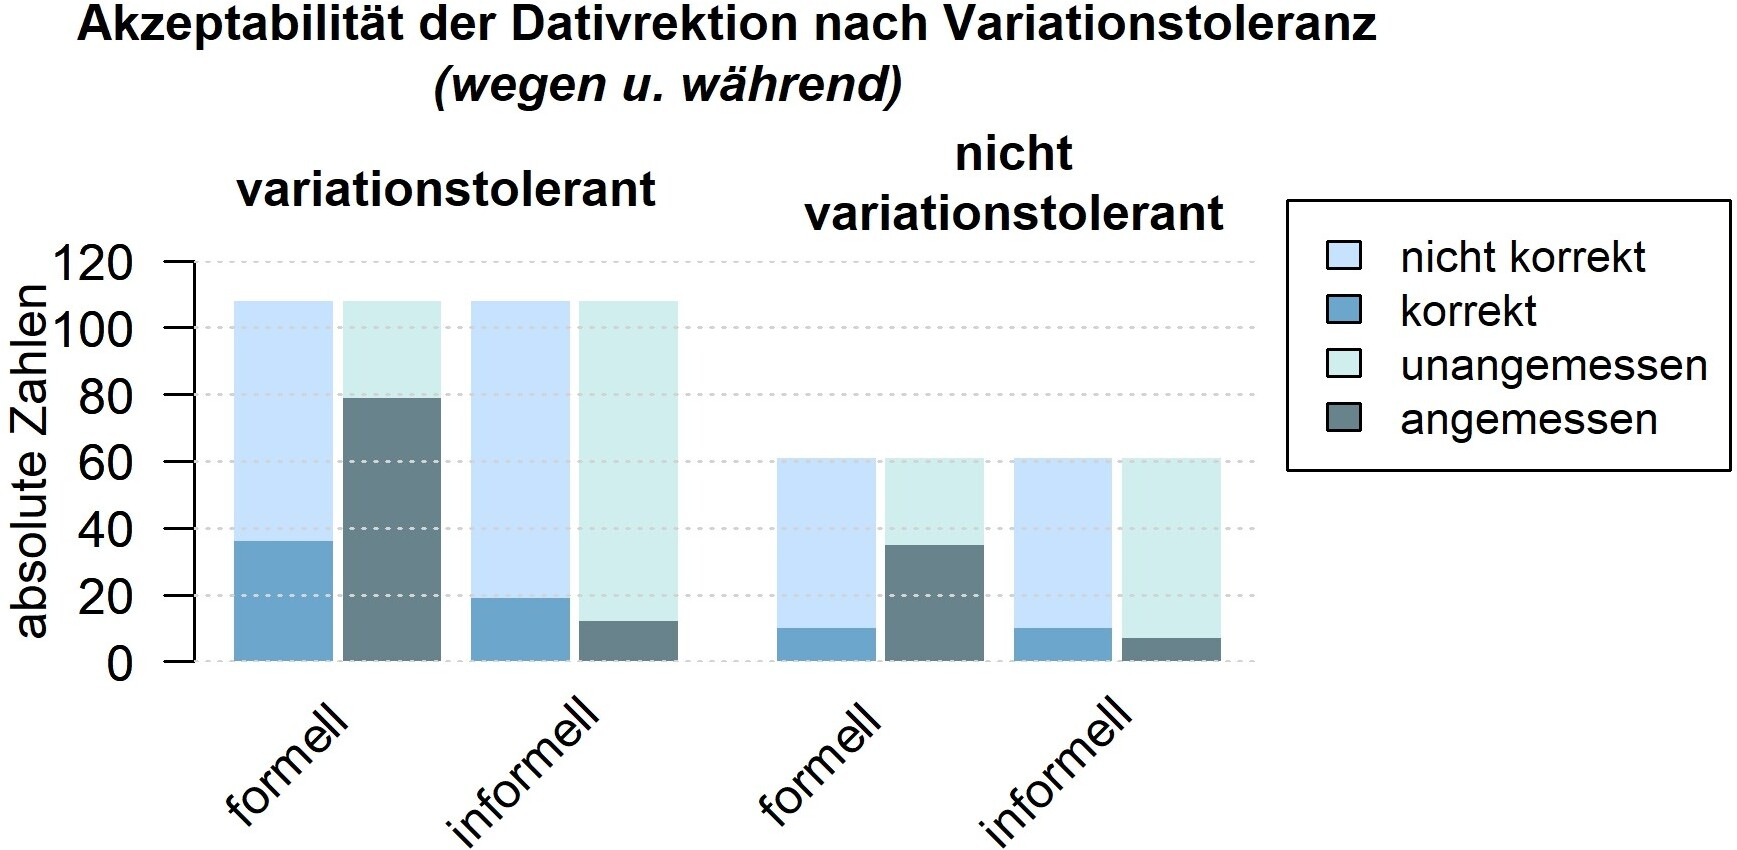
\includegraphics[scale=1]{AkzDativNachVT}
%\caption{Akzeptabilität der Dativrektion bei \wegen{} und \waehrend{} nach Variationstoleranz}
%\label{pic:AkzDativNachVT}
%\end{figure}
%\begin{figure}
%\centering
%\includegraphics[scale=1]{AkzGenitivNAchVT}
%\caption{Akzeptabilität der Genitivrektion bei \dank{} nach Variationstoleranz}
%\label{pic:AkzGenitivNachVT}
%\end{figure}

Bei der Genitivrektion mit der Primärpräposition \object{seit}, die im Akzeptabilitätstest von allen Befragten bewertet wurde, zeigen sich keinerlei Unterschiede zwischen den Gruppen Vt+ und Vt-- (s. \autoref{table:ErgAkzSeitNachVT}). 
% Please add the following required packages to your document preamble:
% \usepackage{multirow}
% \usepackage[table,xcdraw]{xcolor}
% If you use beamer only pass "xcolor=table" option, i.e. \documentclass[xcolor=table]{beamer}
\begin{table}
\centering
\begin{tabular}{llrrrr}
\multicolumn{6}{l}{\object{seit} + Genitiv nach Variationstoleranz}                                                                                                                                                                                                             \\ \hline
                                                                                &                                      & \multicolumn{2}{c}{\begin{tabular}[c]{@{}c@{}}Vt+\\ (n=228)\end{tabular}} & \multicolumn{2}{c}{\begin{tabular}[c]{@{}c@{}}Vt--\\ (n=169)\end{tabular}} \\ \hline
                                                                                & \cellcolor[HTML]{9B9B9B}korrekt      & \cellcolor[HTML]{9B9B9B}72       & \cellcolor[HTML]{9B9B9B}{\footnotesize (31,58 \%)}     & \cellcolor[HTML]{9B9B9B}55       & \cellcolor[HTML]{9B9B9B}{\footnotesize (32,54 \%)}      \\ %\cline{2-6} 
                                                                                & \cellcolor[HTML]{9B9B9B}inkorrekt    & \cellcolor[HTML]{9B9B9B}156      & \cellcolor[HTML]{9B9B9B}{\footnotesize (68,42 \%)}     & \cellcolor[HTML]{9B9B9B}114      & \cellcolor[HTML]{9B9B9B}{\footnotesize (67,46 \%)}      \\ %\cline{2-6} 
                                                                                & \cellcolor[HTML]{EFEFEF}angemessen   & \cellcolor[HTML]{EFEFEF}73       & \cellcolor[HTML]{EFEFEF}{\footnotesize (32,02 \%)}     & \cellcolor[HTML]{EFEFEF}58       & \cellcolor[HTML]{EFEFEF}{\footnotesize (34,32 \%)}      \\ %\cline{2-6} 
                                                                                & \cellcolor[HTML]{EFEFEF}unangemessen & \cellcolor[HTML]{EFEFEF}155      & \cellcolor[HTML]{EFEFEF}{\footnotesize (67,98 \%)}     & \cellcolor[HTML]{EFEFEF}111      & \cellcolor[HTML]{EFEFEF}{\footnotesize (65,68 \%)}      \\ %\cline{2-6} 
                                                                                & eigene Verwendung ja                 & 62                               & {\footnotesize (27,19 \%)}                             & 48                               & {\footnotesize (28,4 \%)}                               \\ %\cline{2-6} 
\multirow{-6}{*}{\begin{tabular}[c]{@{}l@{}}formelles\\ Setting\end{tabular}}   & eigene Verwendung nein               & 166                              & {\footnotesize (72,81 \%)}                             & 121                              & {\footnotesize (71,6 \%)}                               \\ \hline
                                                                                &                                      & \multicolumn{2}{c}{\begin{tabular}[c]{@{}c@{}}Vt+\\ (n=228)\end{tabular}} & \multicolumn{2}{c}{\begin{tabular}[c]{@{}c@{}}Vt--\\ (n=169)\end{tabular}} \\ \hline
                                                                                & \cellcolor[HTML]{9B9B9B}korrekt      & \cellcolor[HTML]{9B9B9B}49       & \cellcolor[HTML]{9B9B9B}{\footnotesize (21,49 \%)}     & \cellcolor[HTML]{9B9B9B}37       & \cellcolor[HTML]{9B9B9B}{\footnotesize (21,89 \%)}      \\ %\cline{2-6} 
                                                                                & \cellcolor[HTML]{9B9B9B}inkorrekt    & \cellcolor[HTML]{9B9B9B}179      & \cellcolor[HTML]{9B9B9B}{\footnotesize (78,51 \%)}     & \cellcolor[HTML]{9B9B9B}132      & \cellcolor[HTML]{9B9B9B}{\footnotesize (78,11 \%)}      \\ %\cline{2-6} 
                                                                                & \cellcolor[HTML]{EFEFEF}angemessen   & \cellcolor[HTML]{EFEFEF}50       & \cellcolor[HTML]{EFEFEF}{\footnotesize (21,93 \%)}     & \cellcolor[HTML]{EFEFEF}44       & \cellcolor[HTML]{EFEFEF}{\footnotesize (26,04 \%)}      \\ %\cline{2-6} 
                                                                                & \cellcolor[HTML]{EFEFEF}unangemessen & \cellcolor[HTML]{EFEFEF}178      & \cellcolor[HTML]{EFEFEF}{\footnotesize (78,07 \%)}     & \cellcolor[HTML]{EFEFEF}125      & \cellcolor[HTML]{EFEFEF}{\footnotesize (73,96 \%)}      \\ %\cline{2-6} 
                                                                                & eigene Verwendung ja                 & 28                               & {\footnotesize (12,28 \%)}                             & 23                               & {\footnotesize (13,61 \%)}                              \\ %\cline{2-6} 
\multirow{-6}{*}{\begin{tabular}[c]{@{}l@{}}informelles\\ Setting\end{tabular}} & eigene Verwendung nein               & 200                              & {\footnotesize (87,72 \%)}                             & 146                              & {\footnotesize (86,39 \%)}                              \\ \hline
\end{tabular}
\caption{Akzeptabilität der Genitivrektion bei \object{seit} nach Variationstoleranz}
\label{table:ErgAkzSeitNachVT}
\end{table}

Insgesamt zeigt der Vergleich der Akzeptabilitätswerte anhand der Variationstoleranz der Befragten, dass die Dativrektion bei \wegen{} und \waehrend{} unter Befragten mit höherer Variationstoleranz im informellen Setting akzeptierter ist als unter Befragten mit geringerer Variationstoleranz.  
Befragte der Gruppe Vt+ bewerten die Varianten hier anteilig häufiger als korrekt und angemessen und würden sie eher selbst verwenden. 
Zudem zeigt sich, dass die Gruppe Vt+ bei der Bewertung der Korrektheit von \wegen{} oder \waehrend{} plus Dativ kontextsensitiver ist: 
Im formellen Setting beurteilen deutlich weniger die Formen als korrekt als im informellen Setting. 
\object{Dank} plus Genitiv scheinen Befragte der Gruppe Vt+ im formellen Setting hingegen eher angemessen zu finden als Befragte der Gruppe Vt--. 
Umgekehrt wertet die Gruppe Vt-- den Genitiv bei \gegenueber{} im formellen Setting eher als angemessen als die Gruppe Vt+. 
Die Primärpräposition \object{seit} mit dem Genitiv wird in beiden Gruppen gleich beurteilt. 
\subsection{\textit{Conditional Inference Trees} und \textit{Random Forests} für den Akzeptabilitätstest}
\label{sec:ErgAkzCTrees}
Bisher wurden folgende mögliche Einflussfaktoren für die Akzeptabilität der Rektionsvarianten besprochen: 
Die Formalität des Kontextes (\autoref{sec:ErgAkzallg}), das Alter der Befragten (\autoref{sec:ErgAkzNachAlter}), die regionale Herkunft (\autoref{sec:ErgAkzNachRegion}), der Bildungsstand (\autoref{sec:ErgAkzNachBildung}), die Textaffinität des Berufs (\autoref{sec:ErgAkzNachBeruf}) und wie variationstolerant die Befragten sind (\autoref{sec:ErgAkzNachVT}).%Änderung Anfang
\footnote{Mögliche Einflüsse des Geschlechts werden nicht untersucht, da die Rektionsvarianten von den Befragten nicht mit Geschlechterkategorien assoziiert werden und das Geschlecht somit keine Ethnokategorie darstellt.} 
% Änderung Ende
Darüber, welche dieser Faktoren sich tatsächlich darauf auswirken, wie Befragte die Varianten im Akzeptabilitätstest bewerten, können statistische Modelle Aufschluss geben. 
Statistische Modelle dienen dazu, zu überprüfen, welche der getesteten unabhängigen Variablen (bspw. Bildungsstand) einen systematischen Einfluss auf eine abhängige Variable haben. 
Die abhängigen Variablen sind im Akzeptabilitätstest die Bewertung der Korrektheit, die Bewertung der Angemessenheit und die Angabe zur eigenen Verwendung. 
Für diese sollen im Folgenden je getrennte statistische Modelle gerechnet werden. 
Ein Modell soll also bspw. die Frage beantworten, wovon es maßgeblich abhängt, ob jemand die im Akzeptabilitätstest präsentierten Varianten als angemessen oder unangemessen beurteilt. 
Dies können \textit{Conditional Inference Trees} und \textit{Random Forests} leisten (\citealp[s.][]{Tagliamonte.2012}; \citealp[291]{Levshina.2015}). 
\textit{Conditional Inference Trees} spalten die Daten anhand der Ausprägungen einer unabhängigen Variable in Gruppen. 
Für die unabhängige Variable \glqq Bildungsstand\grqq{} werden die Daten bspw. in die Gruppe der Befragten mit Hochschulabschluss und die der Befragten ohne Hochschulabschluss gespalten. 
Auch bei Variablen mit mehr als zwei Ausprägungen werden die Daten in zwei Gruppen geteilt, indem zunächst die Fälle mit einer Ausprägung von denen aller anderen Ausprägungen getrennt werden \citep[s.][291]{Levshina.2015}. 
Das Modell überprüft dann, ob sich die Ergebnisse in den beiden Gruppen unterscheiden, ob also bspw. der höchste Bildungsabschluss der Befragten eine gute Vorhersage über ihre Bewertung der Angemessenheit einer Variante zulässt \citep[s.][159]{Tagliamonte.2012}. 
Dies geschieht mithilfe von Permutation: 
Die im Akzeptabilitätstest erhobenen Antworten werden zufällig auf die Befragten verteilt, sodass ein möglicher Zusammenhang zwischen ihnen und dem Bildungsstand aufgebrochen ist. 
Dies wird mehrfach wiederholt, sodass eine ganze Reihe permutierter Datensätze entsteht. 
Anschließend wird kontrolliert, ob sich die tatsächliche Verteilung der abhängigen Variable besser vorhersagen lässt als die zufällig erzeugten Verteilungen \citep[s.][292]{Levshina.2015}.
Ist dies der Fall, besteht offenbar ein Zusammenhang zwischen den Variablen, die Nullhypothese (kein Zusammenhang) kann also abgelehnt werden. 
Der vom Modell ausgegebene p-Wert spiegelt den Anteil der Permutationen wider, bei denen die zufällige Verteilung der Daten ähnlich war wie die der tatsächlich erhobenen Daten \citep[s.][292]{Levshina.2015}. 
Ist er niedrig, kann davon ausgegangen werden, dass sich das Muster in den Daten nicht zufällig ergeben hat. 
Da es sich um eine explorative statistische Analyse handelt, ist die Aussagekraft der p-Werte jedoch eingeschränkt. 

Das beschriebene Vorgehen wird für jede der unabhängigen Variablen wiederholt. 
Auf diese Weise wählt das Modell die unabhängige Variable aus, die den größten Effekt zeigt \citep[s.][291]{Levshina.2015}.
Innerhalb der beiden Gruppen, in die diese Variable die Daten teilt (bspw. Befragte mit vs. ohne Hochschulabschluss) wird anschließend auf die gleiche Art und Weise nach weiteren Einflussfaktoren gesucht. 
Die Daten werden also nach und nach in immer kleinere Gruppen geteilt, die sich in immer mehr Variablenausprägungen unterscheiden. 
So entsteht die Baumstruktur, die dem Modell seinen Namen verleiht \citep[s.][291]{Levshina.2015}.

Ein \textit{Random Forest} besteht aus vielen \textit{Conditional Inference Trees} \citep[s.][292]{Levshina.2015}. 
Da sich mehrere Bäume zu einem Datensatz aufgrund der Permutation voneinander unterscheiden können, hilft der Vergleich vieler \textit{Conditional Inference Trees}, die Relevanz der einzelnen Variablen (\textit{Conditional Variable Importance}) zu ermitteln:
\begin{quote} Random forests can yield the importance measure for every variable in the model averaged over many conditional trees. This measure reflects the impact of each predictor given all other independent variables. \citep[292]{Levshina.2015}\end{quote}
Je größer die \textit{Conditional Variable Importance} einer Variablen im Vergleich zu der anderer Variablen ist, desto größer ist der Einfluss dieser Variable \citep[s.][298--299]{Levshina.2015}. 

\textit{Random Forests} und \textit{Conditional Inference Trees} sind für die hier vorliegenden Daten aus zwei Gründen besonders geeignet. 
Erstens ist eine ihrer Stärken, zu veranschaulichen, wie verschiedene Einflussfaktoren zusammenspielen \citep[s.][135]{Tagliamonte.2012}. 
Mögliche Interaktionen zwischen den einzelnen Variablen (bspw. zwischen Bildungsstand und Alter) werden also nicht nur berücksichtigt, sondern können detailliert analysiert werden \citep[s.][169]{Tagliamonte.2012}. 
Zweitens können \textit{Random Forests} gut mit Datensätzen umgehen, bei denen eine relativ große Zahl möglicher Einflussfaktoren einer relativ kleinen Zahl an Beobachtungen gegenübersteht \citep[s.][161--163]{Tagliamonte.2012}.
Dies ist bei dem vorliegenden Datensatz der Fall:
Die Befragten wurden für den Akzeptabilitätstest auf vier Gruppen verteilt, sodass in jeder Gruppe nur ca. 100 Personen sind. 
Für einige Kombinationen von Ausprägungen der abhängigen Variablen \glqq Angemessenheit\grqq, \glqq Korrektheit\grqq{} und \glqq eigene Verwendung\grqq{} mit Ausprägungen der unabhängigen Variablen sind die Fallzahlen daher sehr gering. 
Bspw. finden sich nur zehn Fälle, in denen jemand aus der Altersgruppe 61--85 den Genitiv bei \dank{} als unangemessen bewertet (\autoref{sec:ErgAkzNachAlter}). 
\citet[]{Tagliamonte.2012} machen anhand von Daten zur \object{was/were}-Variation im Englischen anschaulich, dass sich \textit{Conditional Inference Trees} und \textit{Random Forests} für Datensätze mit wenigen Beobachtungen und vielen Einflussfaktoren, wie sie in der Soziolinguistik häufig zu finden sind, sehr gut eignen. 

Insgesamt wurden zwölf Modelle gerechnet.
\object{Wegen}{} und \waehrend{} wurden aufgrund ihres ähnlichen sprachhistorischen Profils und der geringen Stichprobengröße zusammengefasst (s. dazu auch \autoref{sec:ErgAkzNachAlter}). 
\object{Dank} und \gegenueber{} wurden aufgrund der geringen Vergleichbarkeit (\autoref{cha:SekPraeps}) einzeln behandelt ebenso wie die Primärpräposition \object{seit}.
Es wurden also jeweils vier Baummodelle für die Bewertung der Korrektheit, für die Bewertung der Angemessenheit und für die Angaben zur eigenen Verwendung gerechnet: 
\begin{enumerate}
\item Bewertung der Korrektheit der Dativrektion bei \wegen{} und \waehrend
\item Bewertung der Angemessenheit der Dativrektion bei \wegen{} und \waehrend
\item Angaben zur eigenen Verwendung der Dativrektion bei \wegen{} und \waehrend
\item Bewertung der Korrektheit der Genitivrektion bei \dank
\item Bewertung der Angemessenheit der Genitivrektion bei \dank
\item Angaben zur eigenen Verwendung der Genitivrektion bei \dank
\item Bewertung der Korrektheit der Genitivrektion bei \gegenueber
\item Bewertung der Angemessenheit der Genitivrektion bei \gegenueber
\item Angaben zur eigenen Verwendung der Genitivrektion bei \gegenueber
\item Bewertung der Korrektheit der Genitivrektion bei \object{seit}
\item Bewertung der Angemessenheit der Genitivrektion bei \object{seit}
\item Angaben zur eigenen Verwendung der Genitivrektion bei \object{seit}
\end{enumerate}
%\begin{table}
%\centering
%\begin{tabular}{llll}
%\hline
%                           & \textbf{Korrektheit}         & \textbf{Angemessenheit}      & \textbf{Verwendung}          \\ \hline
%\textbf{wegen und während} & Conditional Inference Tree 1 & Conditional Inference Tree 2 & Conditional Inference Tree 3 \\ \hline
%\textbf{dank}              & Conditional Inference Tree 4 & Conditional Inference Tree 5 & Conditional Inference Tree 6 \\ \hline
%\textbf{gegenüber}         & Conditional Inference Tree 7 & Conditional Inference Tree 8 & Conditional Inference Tree 9 \\ \hline
%\end{tabular}
%%\caption{Conditional Inference Trees für die abhängigen Variablen im Akzeptabilitätstest}
%\label{table:CTrees}
%\end{table}

\noindent \autoref{table:CtreesVariablen} zeigt die jeweils berücksichtigten unabhängigen Variablen und ihre Ausprägungen.
Anders als in den vorherigen Abschnitten (\autoref{sec:ErgAkzNachAlter} bis \autoref{sec:ErgAkzNachVT}) werden für jede Variable alle vorhandenen Ausprägungen berücksichtigt. 
Bspw. werden beim Alter nicht nur die jüngste und die älteste Gruppe verglichen, sondern auch die mittleren Altersgruppen. 
Die Variable \glqq Textaffinität Beruf\grqq{} wurde in den Modellen für eine bessere Darstellbarkeit zu \glqq Beruf\grqq{} abgekürzt. 
%Änderung Anfang
\begin{table}
\centering
\begin{tabular}{ll}
\textbf{Variable}  & \textbf{Ausprägungen}                                                                                   \\ \hline
Setting           & formell, informell
\\ %\hline
Alter              & 18--25, 26--35, 36--60, 61--85                                                                              \\ %\hline
Herkunft           & Nord, Süd, West/Südwest, Ost/Nordost                                                                                    \\ %\hline
Bildungsstand            & \begin{tabular}[c]{@{}l@{}}Hochschulabschluss, kein Hochschulabschluss \end{tabular} 
\\ %\hline
Textaffinität Beruf           & textaffin, nicht textaffin 
\\ %\hline
Variationstoleranz & hoch, gering                                                                                           
\\ %\hline
KandidatIn & 1 bis 397                                                                                            \\ 
\end{tabular}
\caption{Einflussfaktoren im Akzeptabilitätstest und ihre Ausprägungen}
\label{table:CtreesVariablen}
\end{table}
% Änderung Ende

In alle Modelle wurde die Variable \glqq KandidatIn\grqq{} mit aufgenommen.
Dies ist nötig, da jeweils zwei Antworten zu jeder der abhängigen Variablen (Korrektheit, Angemessenheit und Verwendung) von ein und derselben Person stammen. 
Da es möglich ist, dass die Akzeptabilität der Varianten vornehmlich von der generellen Vorliebe einer Person für einen Kasus abhängt, soll dies durch das Modell überprüft werden. 
Im Falle der Modelle für die Dativrektion bei \wegen{} und \waehrend{} wurde außerdem die Variable \glqq Präposition\grqq{} mit den Ausprägungen \glqq \wegen{}\grqq{} und \glqq \waehrend{}\grqq{} einbezogen. 
Auf diese Weise kann das Modell kontrollieren, ob die Akzeptabilitätsentscheidungen der Befragten bei der Dativrektion von der Präposition abhängen. 

Die \textit{Conditional Inference Trees} und \textit{Random Forests} wurden mit dem Paket party in R gerechnet \citep[][Version 1.3-4]{Hothorn.2010}.\footnote{Hier beispielhaft der in RStudio eingegebene Code für den \textit{Conditional Inference Tree} sowie den \textit{Random Forest} zur Bewertung der Korrektheit der Dativrektion:\\
\texttt{\# Conditional Inference Tree \\
KorrDat.ctree = ctree(Korrektheit \$ Kandidat + Setting + Praep + Bildung + Herkunft + Altersgruppe + Variationstoleranz, controls = ctree\_control(minbucket=10), data = AkzDativr)\\
\# Random Forest \\
data.controls = cforest\_unbiased(ntree=1000,mtry=2)\\
forestDativVerw = cforest(Verwendung \$ KandidatIn + Setting + Praep + Altersgruppe + Herkunft + Bildung + Beruf + Variationstoleranz, AkzDativr, controls = data.controls)}
}
In den Einstellungen zu den \textit{Conditional Inference Trees} wurde festgelegt, dass jede vom Modell gebildete Gruppe (jedes \glqq Blatt\grqq) mindestens zehn Fälle umfasst. 
In den Befehlen für die \textit{Random Forests} wurde angegeben, dass für einen \textit{Forest} jeweils 1000 \textit{Trees} gerechnet werden. 
Außerdem legen die Einstellungen fest, dass für jeden Split drei zufällig ausgewählte Prädiktoren herangezogen werden \citep[s.][297]{Levshina.2015}.
Wie gut die \textit{Random Forests} die Daten jeweils repräsentieren, kann über den C-Wert ermittelt werden, der zwischen 0 und 1 liegt \citep[s.][299]{Levshina.2015}. 
Dieser wurde in R mithilfe des Pakets Hmisc berechnet \citep[][Version 4.4-0]{Harrell.2020}.
C-Werte über 0,8 bedeuten laut \citet[156]{Tagliamonte.2012} eine gute Passung des Modells auf die Daten. 

Der \textit{Conditional Inference Tree} für die Bewertung der Korrektheit von \wegen{} und \waehrend{} plus Dativ zeigt, dass die Herkunft der Befragten die Wahrscheinlichkeit beeinflusst, mit der sie die Variante als korrekt beurteilen (s. \autoref{pic:CtreeKorrDativr}). 
Für süddeutsche Befragte (\textit{Node} 2) ist die Wahrscheinlichkeit, dass sie die Dativrektion als richtig beurteilen, deutlich höher als für Befragte aus anderen Teilen Deutschlands (\textit{Node} 3). 
Weitere Faktoren scheinen keine Rolle zu spielen. 
Der \textit{Random Forest} für die Bewertung der Korrektheit von \wegen{} oder \waehrend{} plus Dativ liefert für den Faktor \glqq Herkunft\grqq{} eine \textit{Conditional Variable Importance} von 0,009, für alle anderen Faktoren liegt sie bei höchstens 0,004. 
Der C-Wert für den \textit{Random Forest} deutet mit 0,86 auf eine gute Passung des Modells hin. 
\begin{figure}
\centering
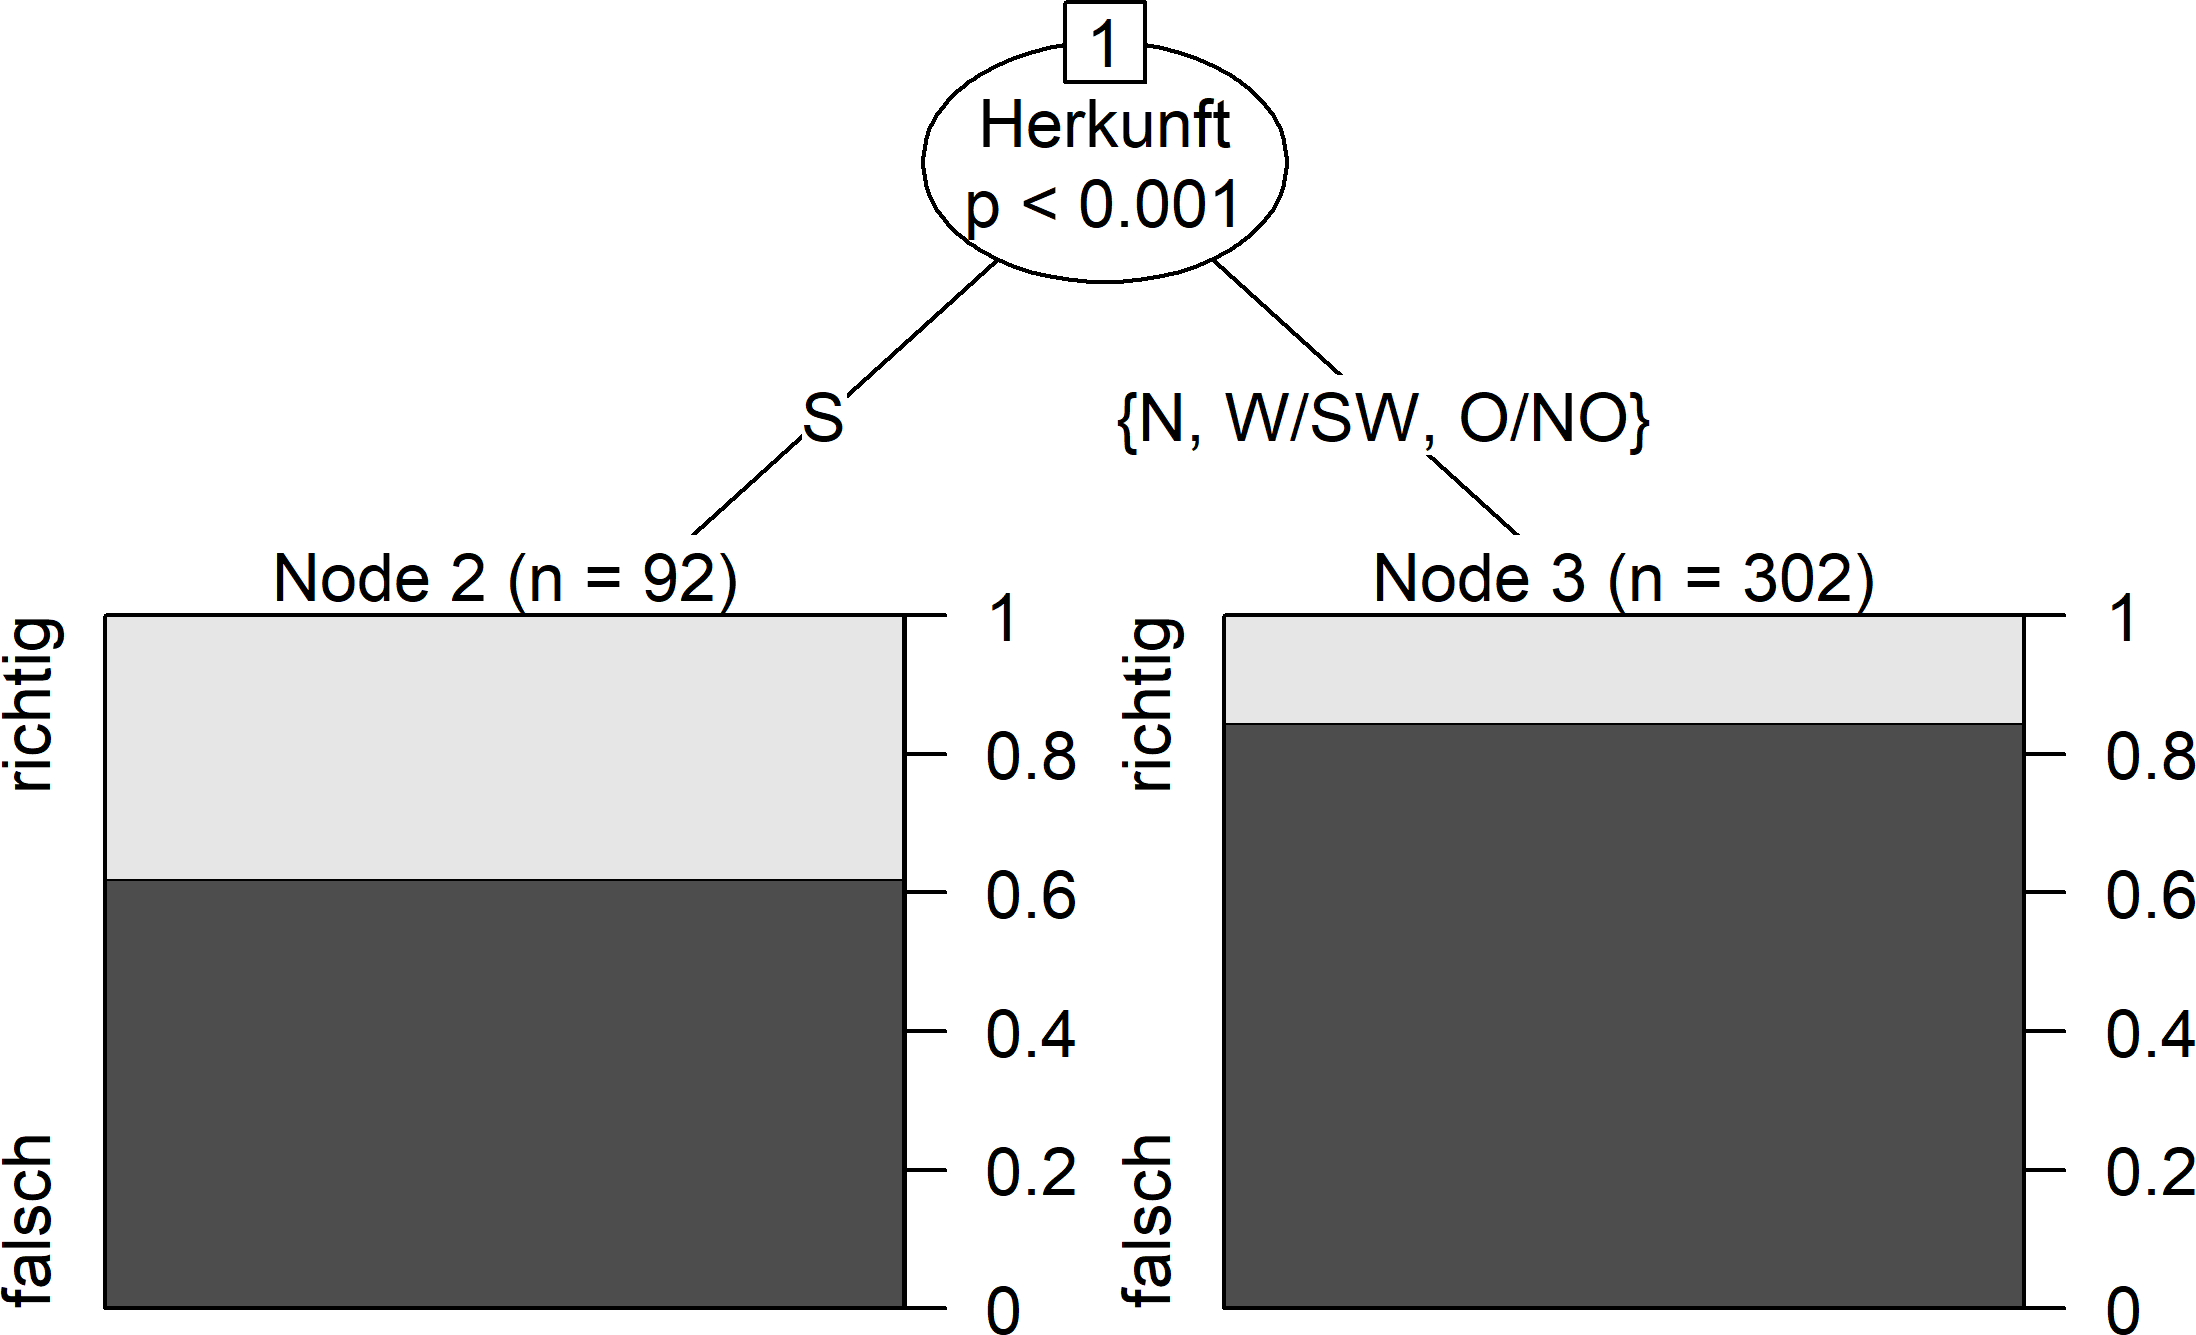
\includegraphics[width=\textwidth]{CtreeDativKorr.png}
\caption{\textit{Conditional Inference Tree} für die Bewertung der Korrektheit der Dativrektion bei \wegen{} und \waehrend}
\label{pic:CtreeKorrDativr}
\end{figure}

Der \textit{Conditional Inference Tree} zur Bewertung der Angemessenheit der Dativrektion bei \wegen{} und \waehrend{} splittet die Daten zunächst anhand des Settings (s. \autoref{pic:CtreeAngDativr}): 
Im formellen Kontext ist die Wahrscheinlichkeit für die Einstufung als unangemessen unter allen Befragten höher als im informellen Setting. 
Im informellen Setting hingegen urteilen norddeutsche Befragte dem Modell zufolge anders als Befragte aus dem restlichen Deutschland. 
%Änderung Anfang
Während für Norddeutsche eine Wahrscheinlichkeit von rund 0,5 vorhergesagt wird, dass sie die Variante auch in einem Gespräch mit einem Freund als unangemessen einstufen, ist unter den Befragten aus Süd-, West- bzw. Südwest und Ost- bzw. Nordostdeutschland die Wahrscheinlichkeit hoch, dass sie die Dativrektion hier als angemessen bewerten. 
% Änderung Ende
Mit einer \textit{Variable Importance} von 0,013 ist der Einfluss der Herkunft auf die Beurteilung der Angemessenheit allerdings deutlich geringer als der des Settings (\textit{Variable Importance} von 0,167). 
Die Passung des \textit{Random Forests} ist mit 0,92 sehr gut. 
\begin{figure}
\centering
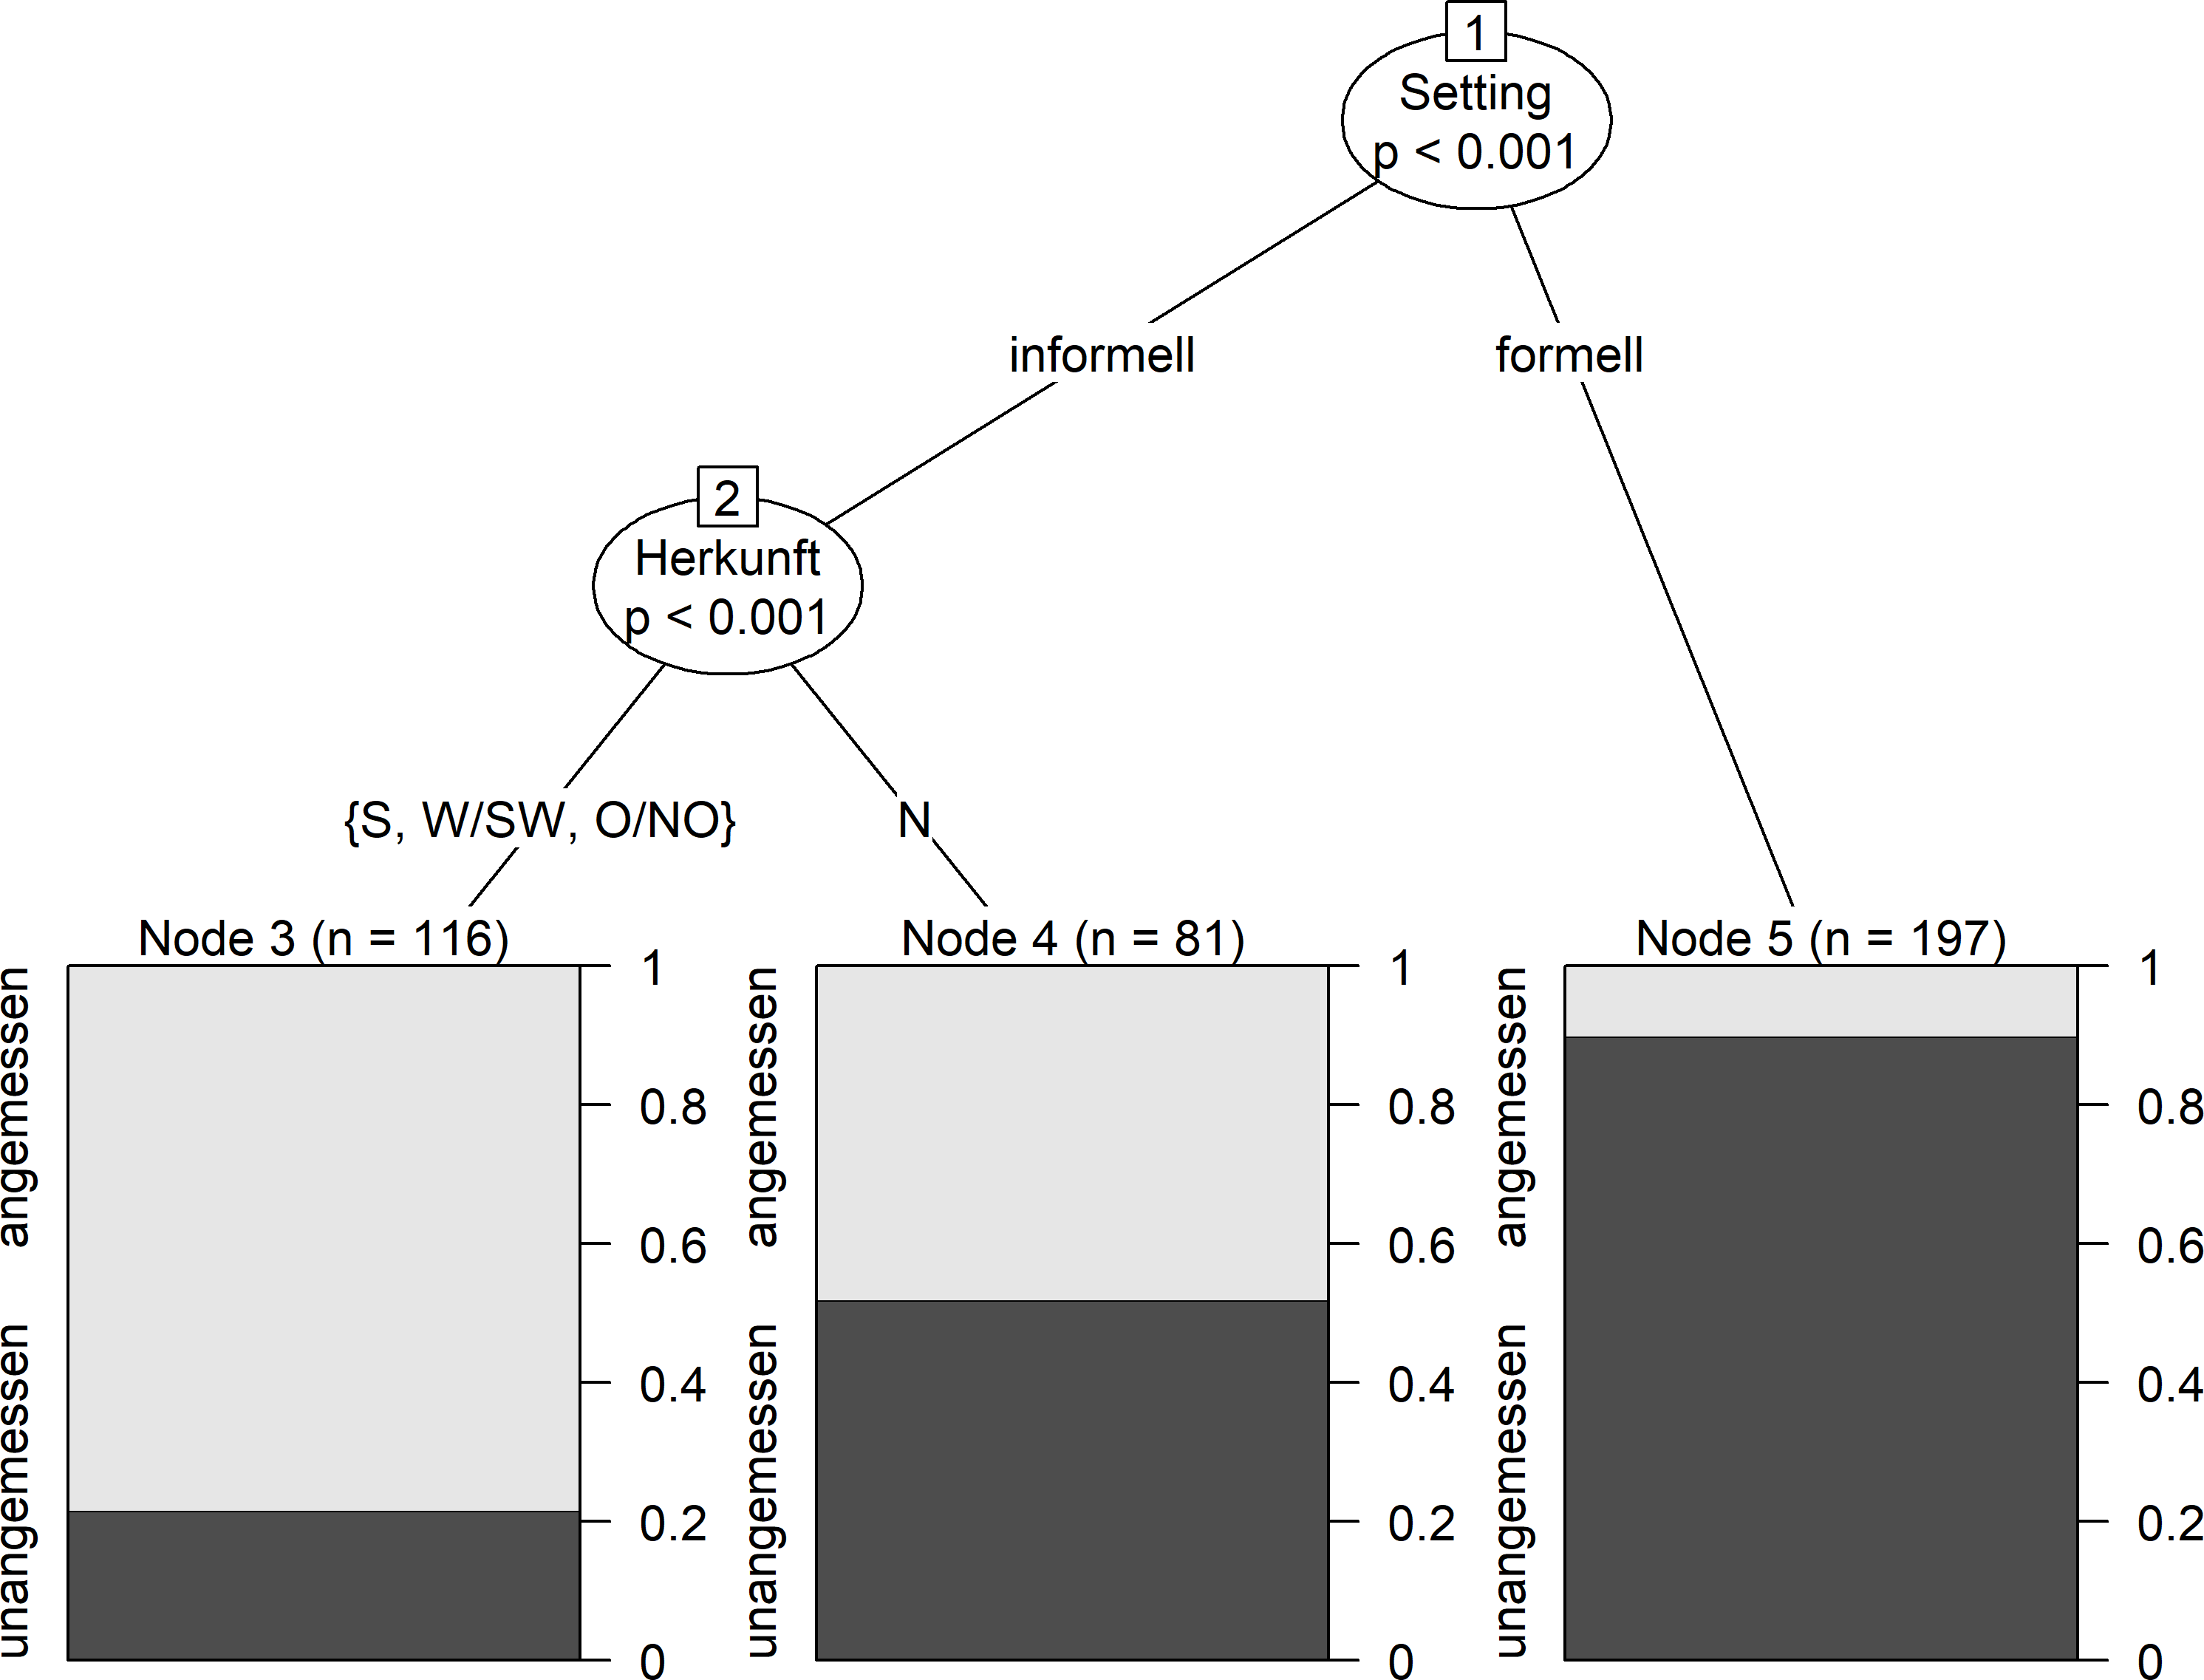
\includegraphics[width=\textwidth]{CtreeDativAng.png}
\caption{\textit{Conditional Inference Tree} für die Bewertung der Angemessenheit der Dativrektion bei \wegen{} und \waehrend}
\label{pic:CtreeAngDativr}
\end{figure}

Auch für die Angabe, ob Befragte die Dativrektion selbst verwenden würden, ist zunächst die Formalität des Settings ausschlaggebend (s. \autoref{pic:CtreeVerwDativr}). 
In einem Brief an ein Amt (formelles Setting) sagt das Modell für alle Befragten eine hohe Wahrscheinlichkeit voraus, den Dativ für die eigene Verwendung abzulehnen. 
Im informellen Setting spielt auch bei der Angabe zur eigenen Verwendung wieder die Herkunft eine Rolle (s. \textit{Node} 2). 
% Änderung Anfang
Dieses Mal stehen die Befragten aus süd- und west- bzw. südwestdeutschen Bundesländern den Befragten aus nord- und ost- bzw. nordostdeutschen Bundesländern gegenüber.
% Änderung Ende 
Für die Nord- und Ost- bzw. Nordostdeutschen sagt das Modell mit einer Wahrscheinlichkeit von rund 0,7 voraus, dass sie die Dativrektion auch im informellen Setting nicht verwenden würden. 
Bei Befragten aus Süd- und West- bzw. Südwestdeutschland hängt es von ihrer Variationstoleranz ab, wie wahrscheinlich es ist, dass sie den Dativ in einem informellen Kontext verwenden würden (s. \textit{Node} 3). 
Für Personen mit einer hohen Variationstoleranz wird mit einer Wahrscheinlichkeit von beinahe 0,9 vorausgesagt, dass sie \wegen{} oder \waehrend{} plus Dativ im Gespräch mit einem Freund verwenden würden. 
Für diejenigen Süd- und West- bzw. Südwestdeutschen, die Variation ablehnend gegenüberstehen, sagt das Modell dies nur mit einer Wahrscheinlichkeit von rund 0,5 vorher. 
Die vom \textit{Random Forest} berechneten \textit{Variable Importances} legen nahe, dass der Einfluss des Settings (0,079) deutlich größer ist als der von Herkunft (0,037) und Variationstoleranz (0,01). 
Der C-Wert beträgt 0,91 und zeigt damit eine sehr gute Passung des Modells auf die Daten an. 
\begin{figure}[p]
\centering
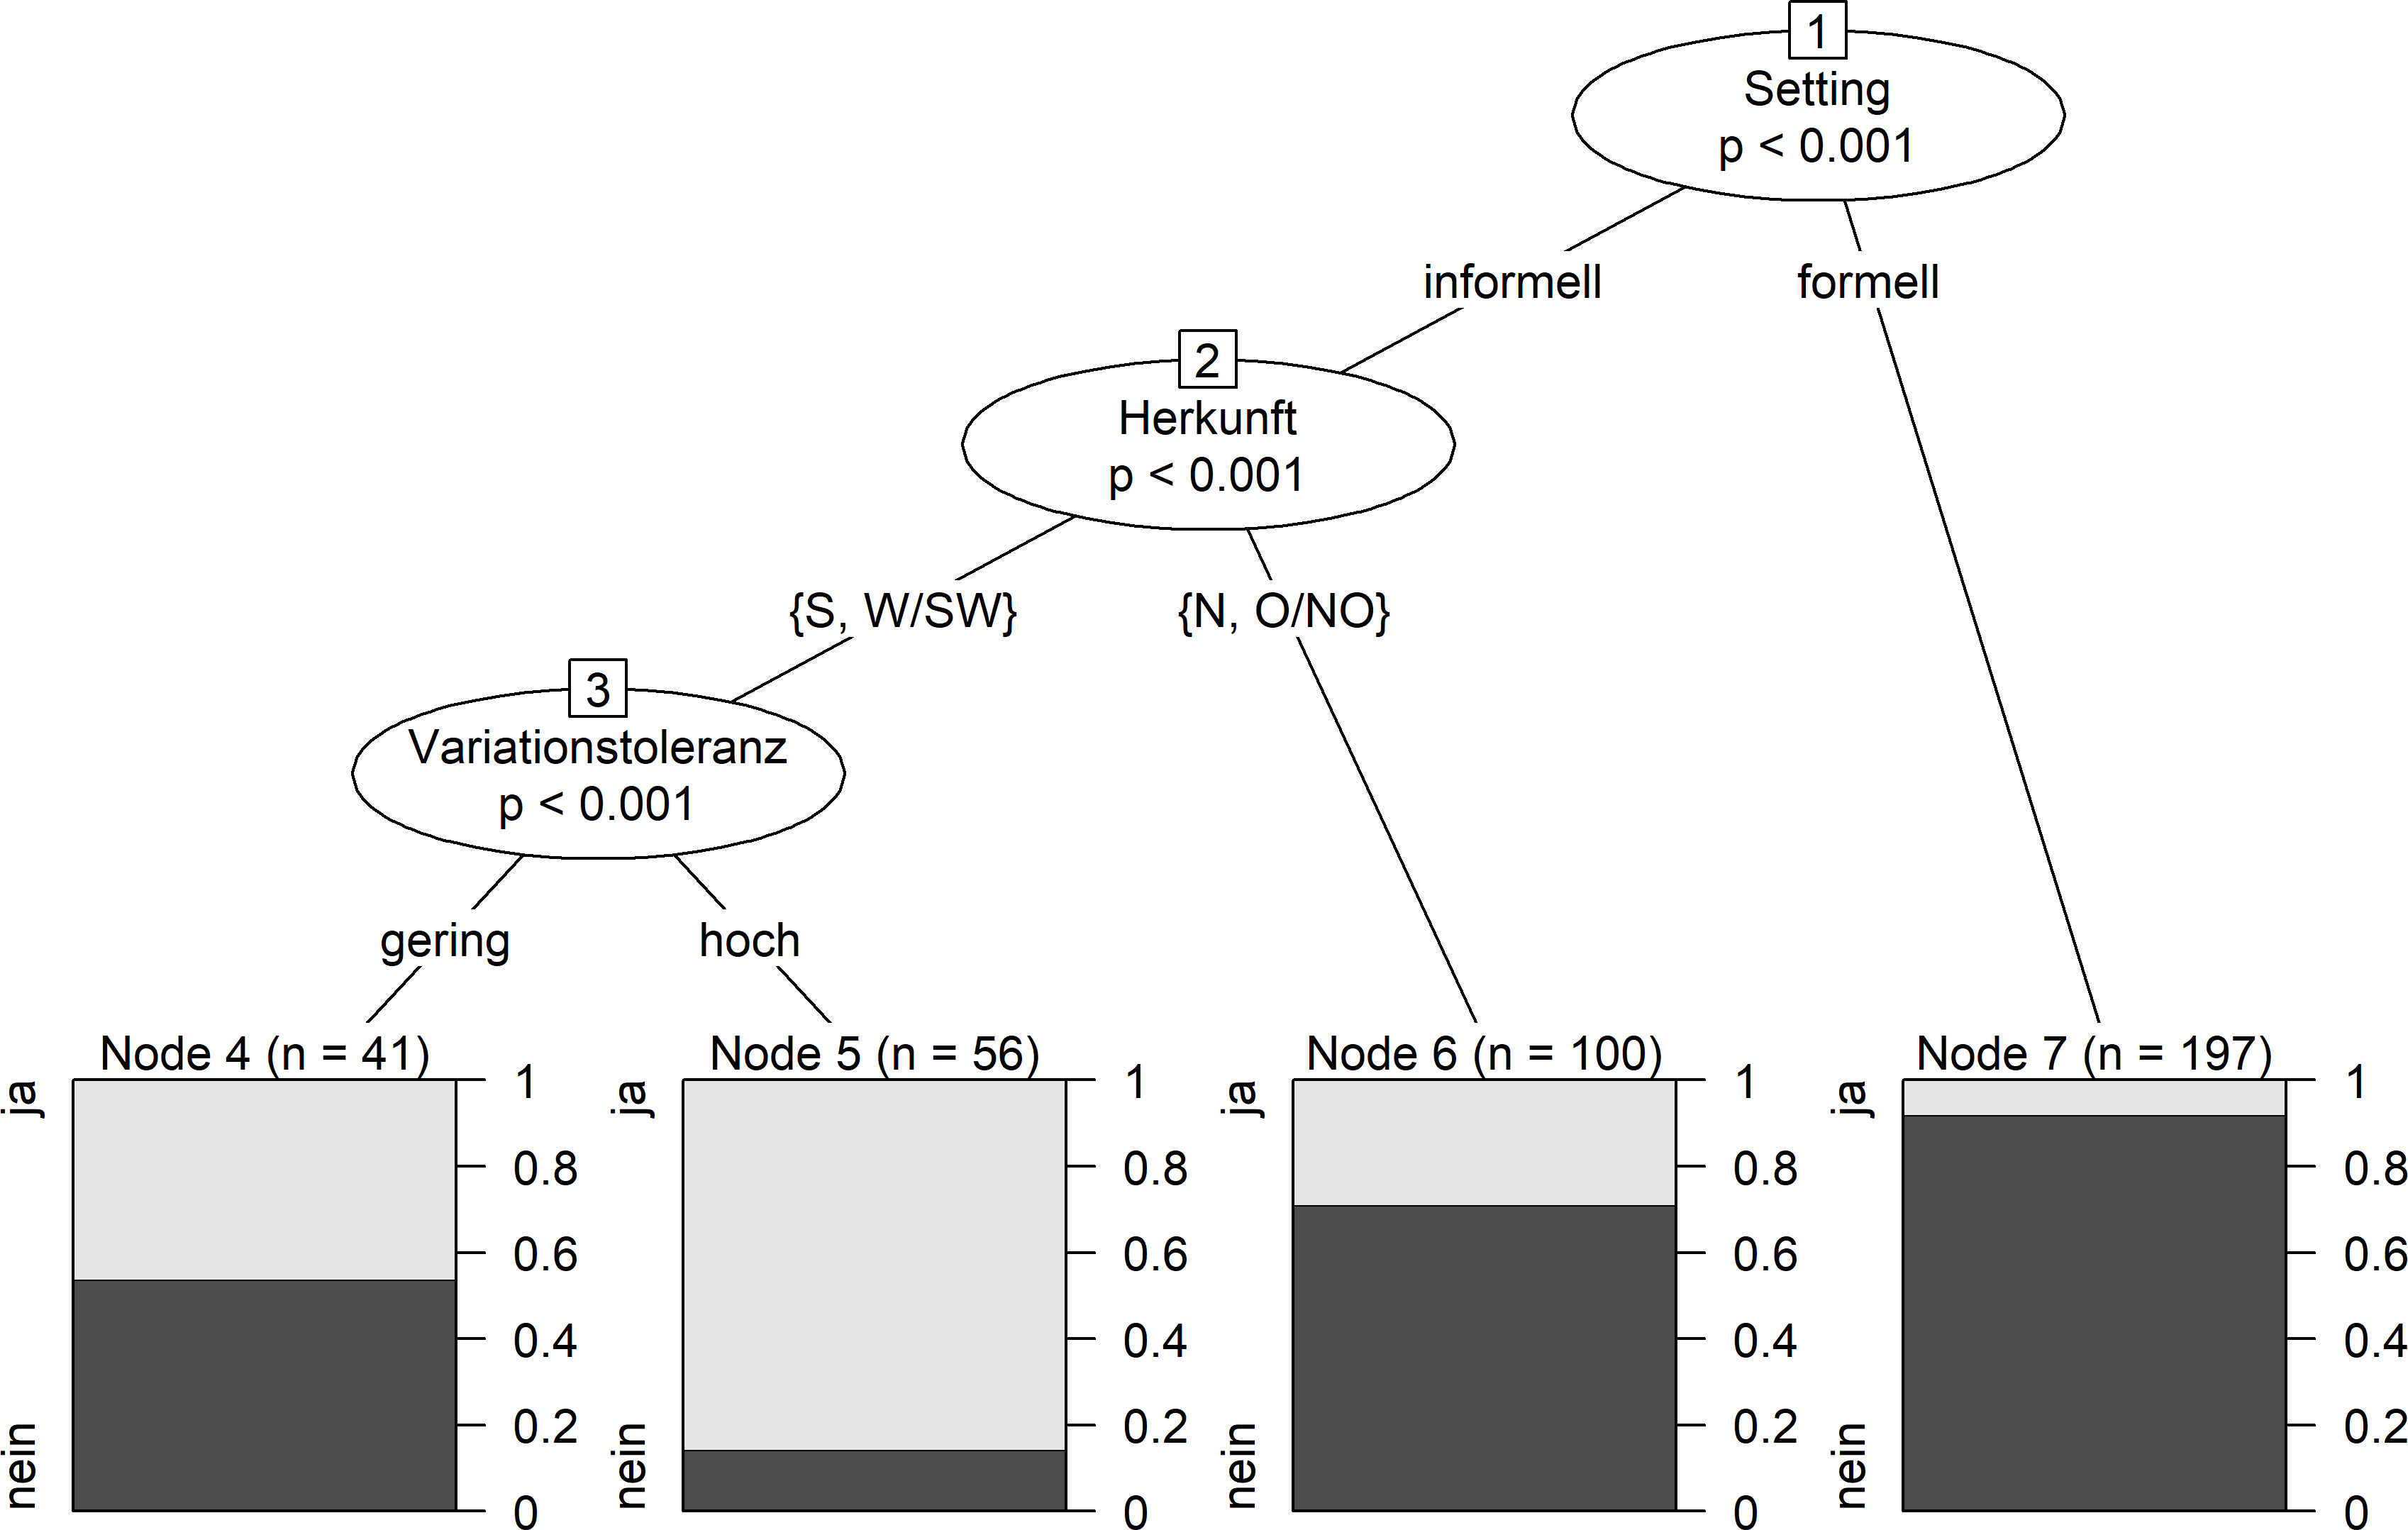
\includegraphics[angle=90, scale=0.7]{CtreeDativVerw.png}
\caption{\textit{Conditional Inference Tree} für die Angaben zur eigenen Verwendung der Dativrektion bei \wegen{} und \waehrend}
\label{pic:CtreeVerwDativr}
\end{figure}

Die \textit{Conditional Inference Trees} zur Genitivrektion bei \dank{} zeigen keinen Split in den Daten.
Alle von den \textit{Random Forests} berechneten \textit{Variable Importances} liegen bei oder sehr nahe bei null.
Das heißt, die Angaben zur Korrektheit, Angemessenheit und eigenen Verwendung von \dank{} plus Genitiv zeigen keine Abhängigkeit von einer der getesteten Variablen. 
Offenbar beurteilen Befragte die Variante unabhängig vom Setting, ihrem Alter, ihrer regionalen Herkunft, ihrem Bildungsstand, der Textaffinität ihres Berufs und ihrer Variationstoleranz häufig als korrekt und angemessen und würden sie selbst verwenden (\autoref{sec:ErgAkzNachAlter} bis \autoref{sec:ErgAkzNachVT}). 
Die C-Werte für die drei \textit{Random Forests} betragen alle über 0,8 und repräsentieren die Daten damit gut.

\object{Gegenüber} wird im Akzeptabilitätstest unabhängig von den getesteten Variablen eher abgelehnt. 
Auch hier werden die Daten von den \textit{Conditional Inference Trees} nicht aufgeteilt. 
Die Passung der \textit{Random Forests} liegt jeweils bei mindestens 0,8, ist also gut. 
Die grafischen Darstellungen der \textit{Conditional Inference Trees} zu \dank{} und \gegenueber{} finden sich im Anhang (s. \autoref{pic:AnhCtreeKorrGenitivrDank} bis \autoref{pic:AnhCtreeVerwGenitivrGegenueber}). 

\autoref{pic:CtreeKorrGenitivrSeit} zeigt den \textit{Conditional Inference Tree} für die Bewertung der Korrektheit der Genitivrektion bei der Primärpräposition \object{seit}.
Er splittet die Daten anhand der Variable \glqq Textaffinität des Berufs\grqq:
Für Befragte aus textaffinen Berufen wird eine geringere Wahrscheinlichkeit vorhergesagt, dass sie \object{seit} plus Genitiv als korrekt beurteilen. 
Der \textit{Random Forest} gibt für die Textaffinität des Berufs eine \textit{Variable Importance} von 0,008 an. 
Im Vergleich dazu liegt der Wert für den Faktor \glqq Altersgruppe\grqq, der keinen Split im \textit{Tree} erzeugt, nur bei 0,004.
Mit einem C-Wert von 0,8 passt das Modell gut auf die Daten. 
\begin{figure}
\centering
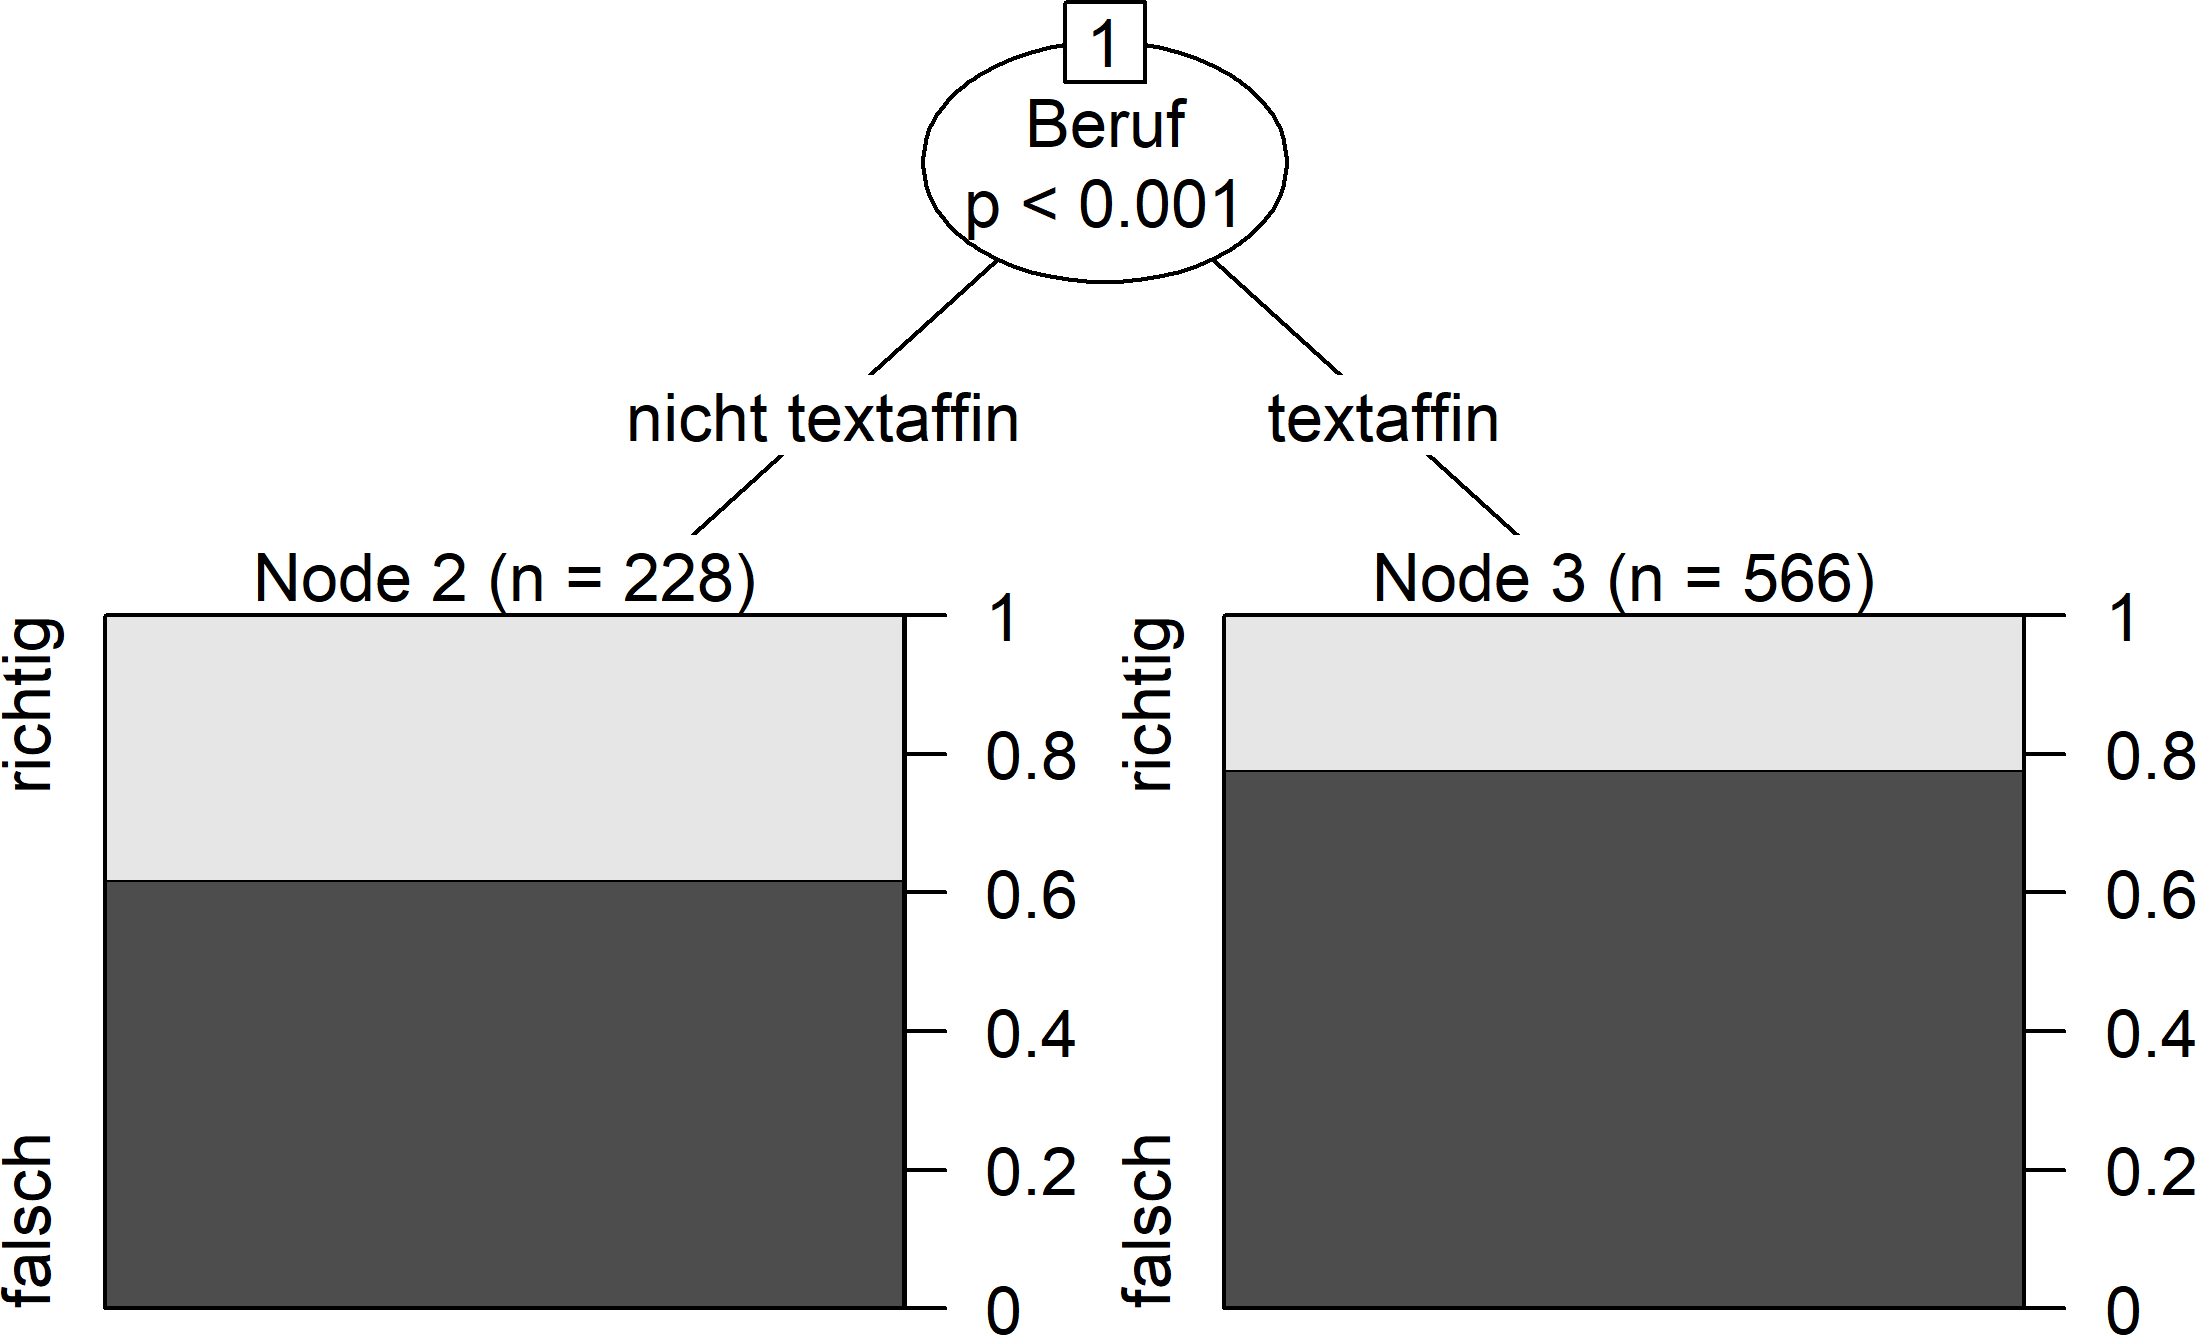
\includegraphics[width=\textwidth]{CtreeGenitivseitKorr.png}
\caption{\textit{Conditional Inference Tree }für die Bewertung der Korrektheit der Genitivrektion bei \object{seit}}
\label{pic:CtreeKorrGenitivrSeit}
\end{figure}

Auch der \textit{Conditional Inference Tree} zur Beurteilung der Angemessenheit von \object{seit} mit dem Genitiv splittet die Daten anhand der Textaffinität des Berufs, wie in \autoref{pic:CtreeAngGenitivrSeit} zu sehen. 
Allerdings liegt die \textit{Variable Importance} der Textaffinität des Berufs hier mit 0,004 sehr nah an der der anderen Faktoren, für die kein Split erzeugt wird. 
Über viele Baummodelle gemittelt scheint sich ihr Einfluss also zu relativieren. 
Der \textit{Random Forest} für die Beurteilung der Angemessenheit von \object{seit} plus Genitiv hat mit 0,81 eine gute Passung. 
\begin{figure}
\centering
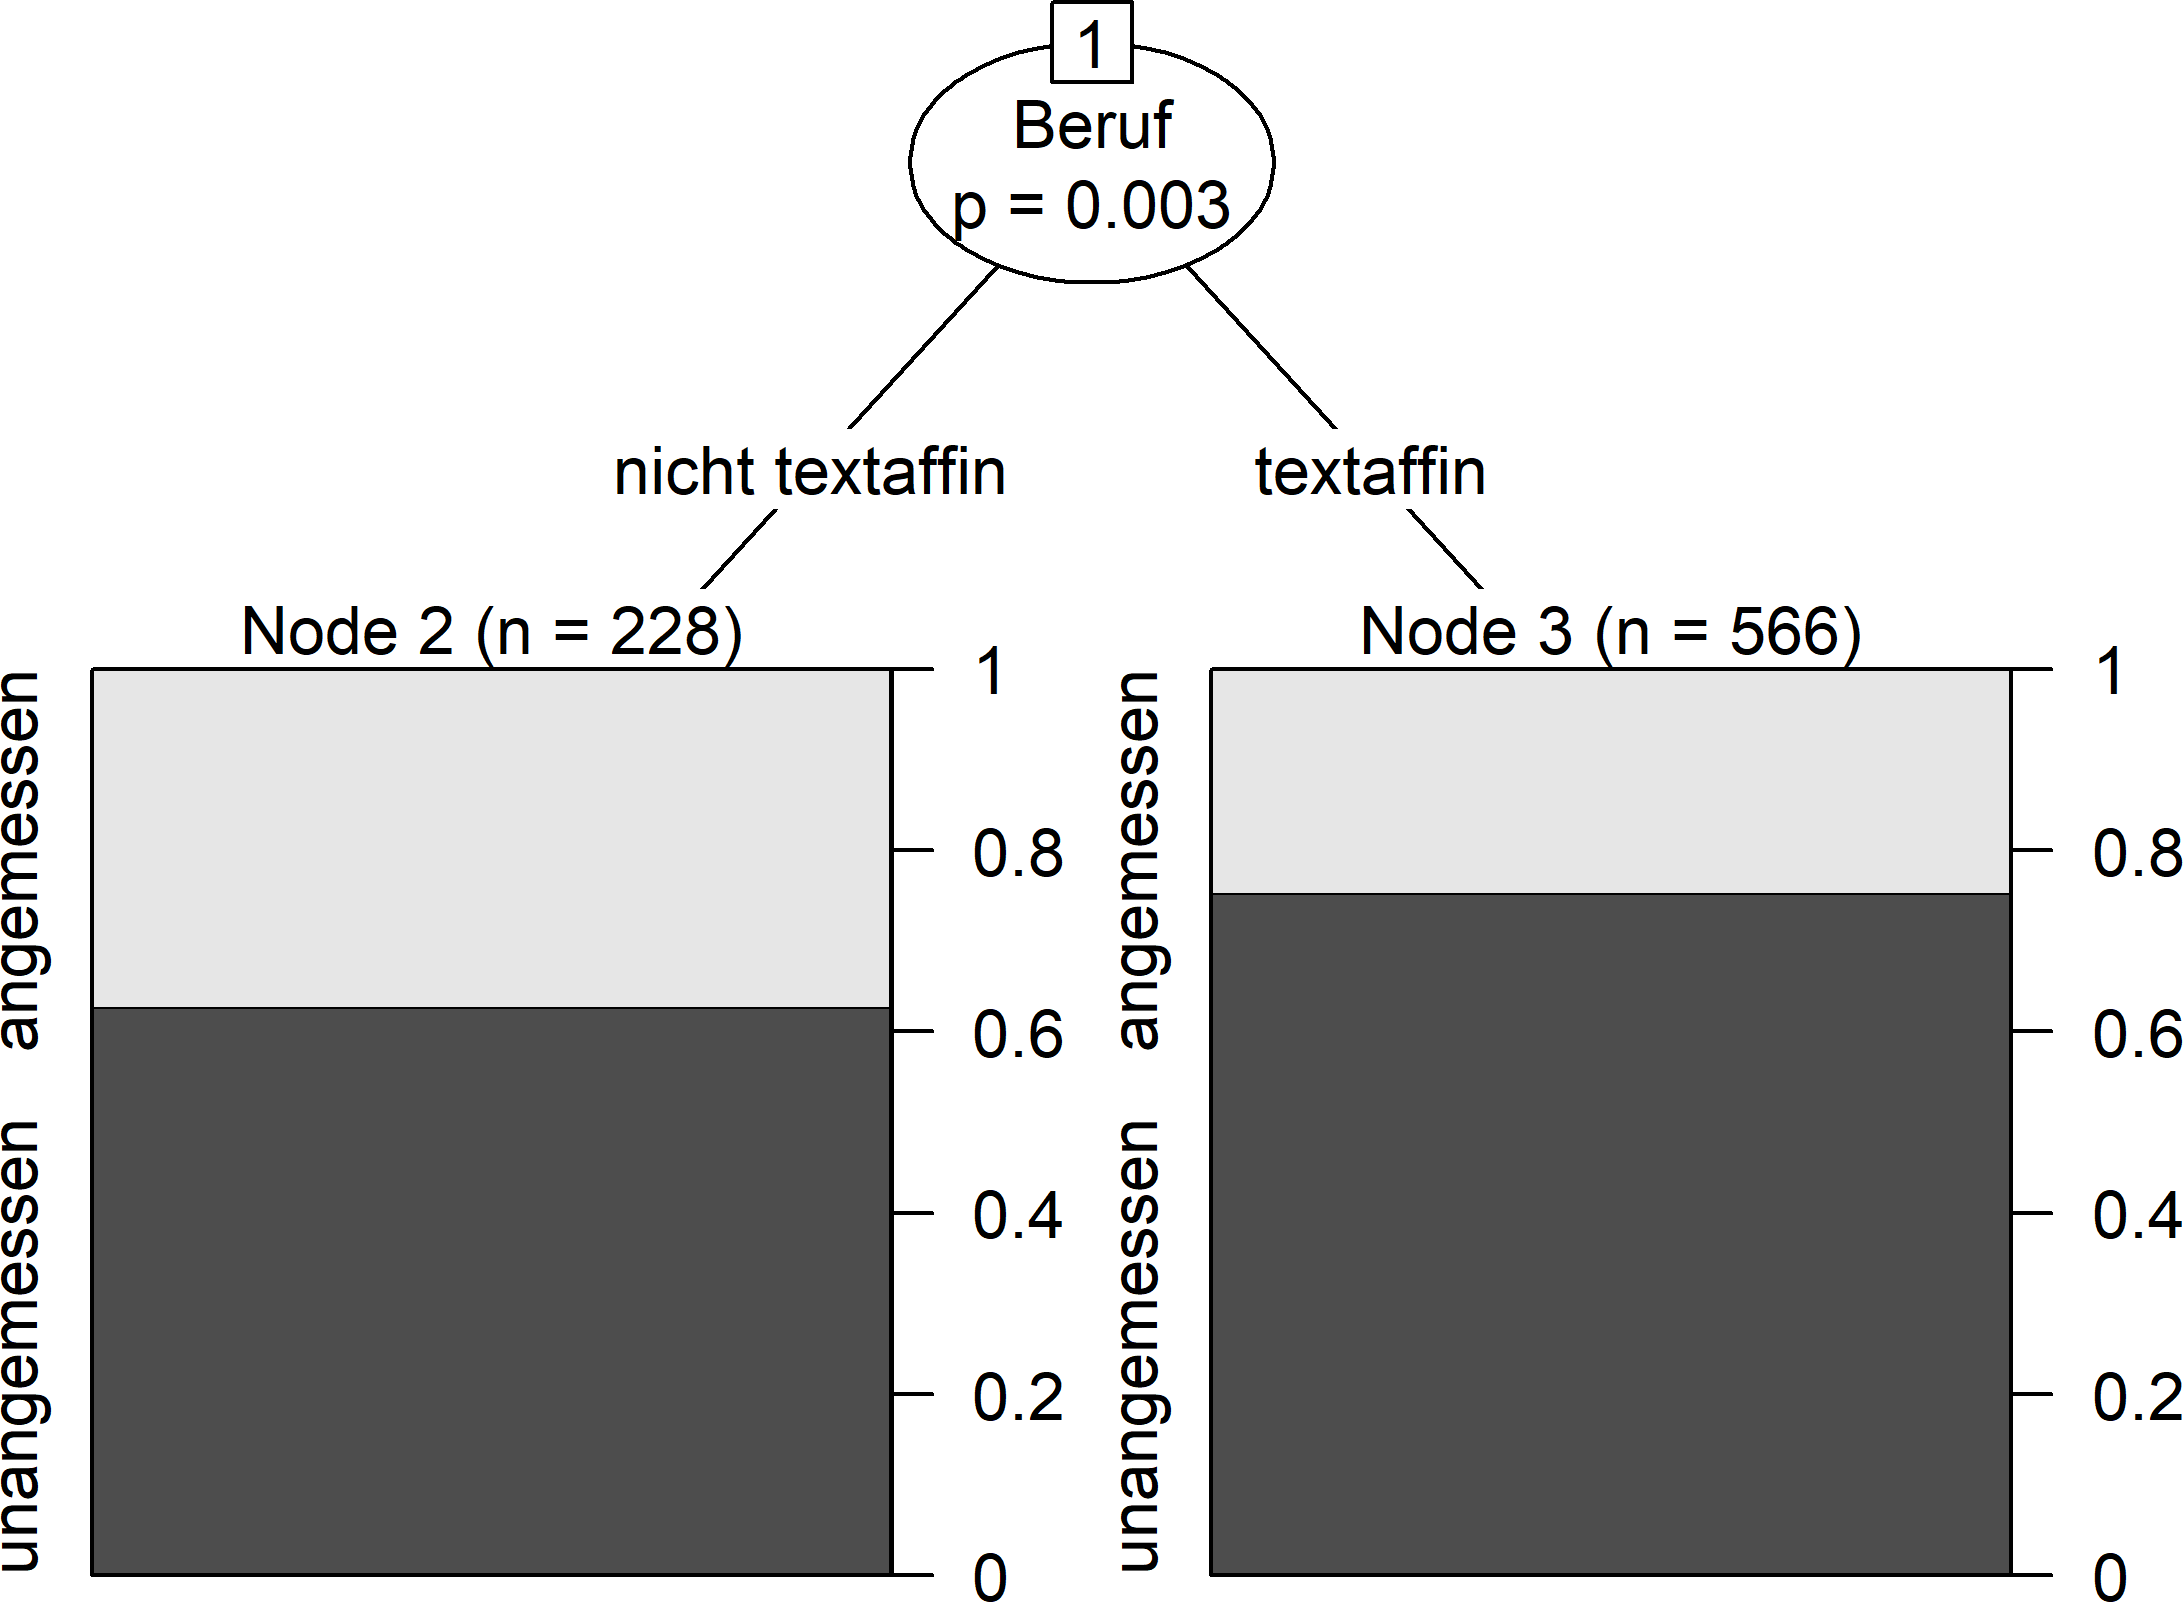
\includegraphics[width=\textwidth]{CtreeGenitivseitAng.png}
\caption{\textit{Conditional Inference Tree} für die Bewertung der Angemessenheit der Genitivrektion bei \object{seit}}
\label{pic:CtreeAngGenitivrSeit}
\end{figure}

In \autoref{pic:CtreeVerwGenitivrSeit} ist der \textit{Conditional Inference Tree} für die Angaben zur eigenen Verwendung der Genitivrektion bei der Primärpräposition \object{seit} dargestellt. 
Der erste Split in den Daten wird hier anhand des Settings erzeugt. 
Anschließend werden die Daten im formellen Setting nach der Textaffinität des Berufs geteilt (s. \textit{Node} 2) und im informellen Setting nach dem Bildungsstand der Befragten (s. \textit{Node} 5). 
Die höchste Wahrscheinlichkeit für die Angabe, die Variante selbst zu verwenden, sagt das Modell für Befragte aus nicht-sprachaffinen Berufen im formellen Setting vorher (s. \textit{Node} 3). 
Für Befragte mit Hochschulabschluss im informellen Setting hingegen ist die Wahrscheinlichkeit, dass sie angeben, \object{seit} plus Genitiv selbst zu verwenden, am geringsten (s. \textit{Node} 7). 
% Änderung Anfang
Höherer Bildungsgrad und höhere Textaffinität des Berufs gehen also mit niedrigeren Werten zur Selbsteinschätzung der Verwendung des Genitivs bei \textit{seit} einher. 
% Änderung Ende
Schaut man sich jedoch die vom \textit{Random Forest} berechneten \textit{Variable Importances} an, liegen diese für die Textaffinität des Berufs und den Bildungsstand mit 0,003 und 0,002 höher als für das Setting und insgesamt sehr nah bei null.
Das Setting hat mit 0,002 eine ebenso hohe \textit{Variable Importance} wie der Faktor \glqq Altersgruppe\grqq, der im \textit{Tree} nicht zu einem Split führt. 
Dies deutet auf eine geringe Aussagekraft des Modells hin. 
Die Passung des \textit{Random Forests} ist mit 0,84 dennoch gut. 
\begin{figure}[p]
\centering
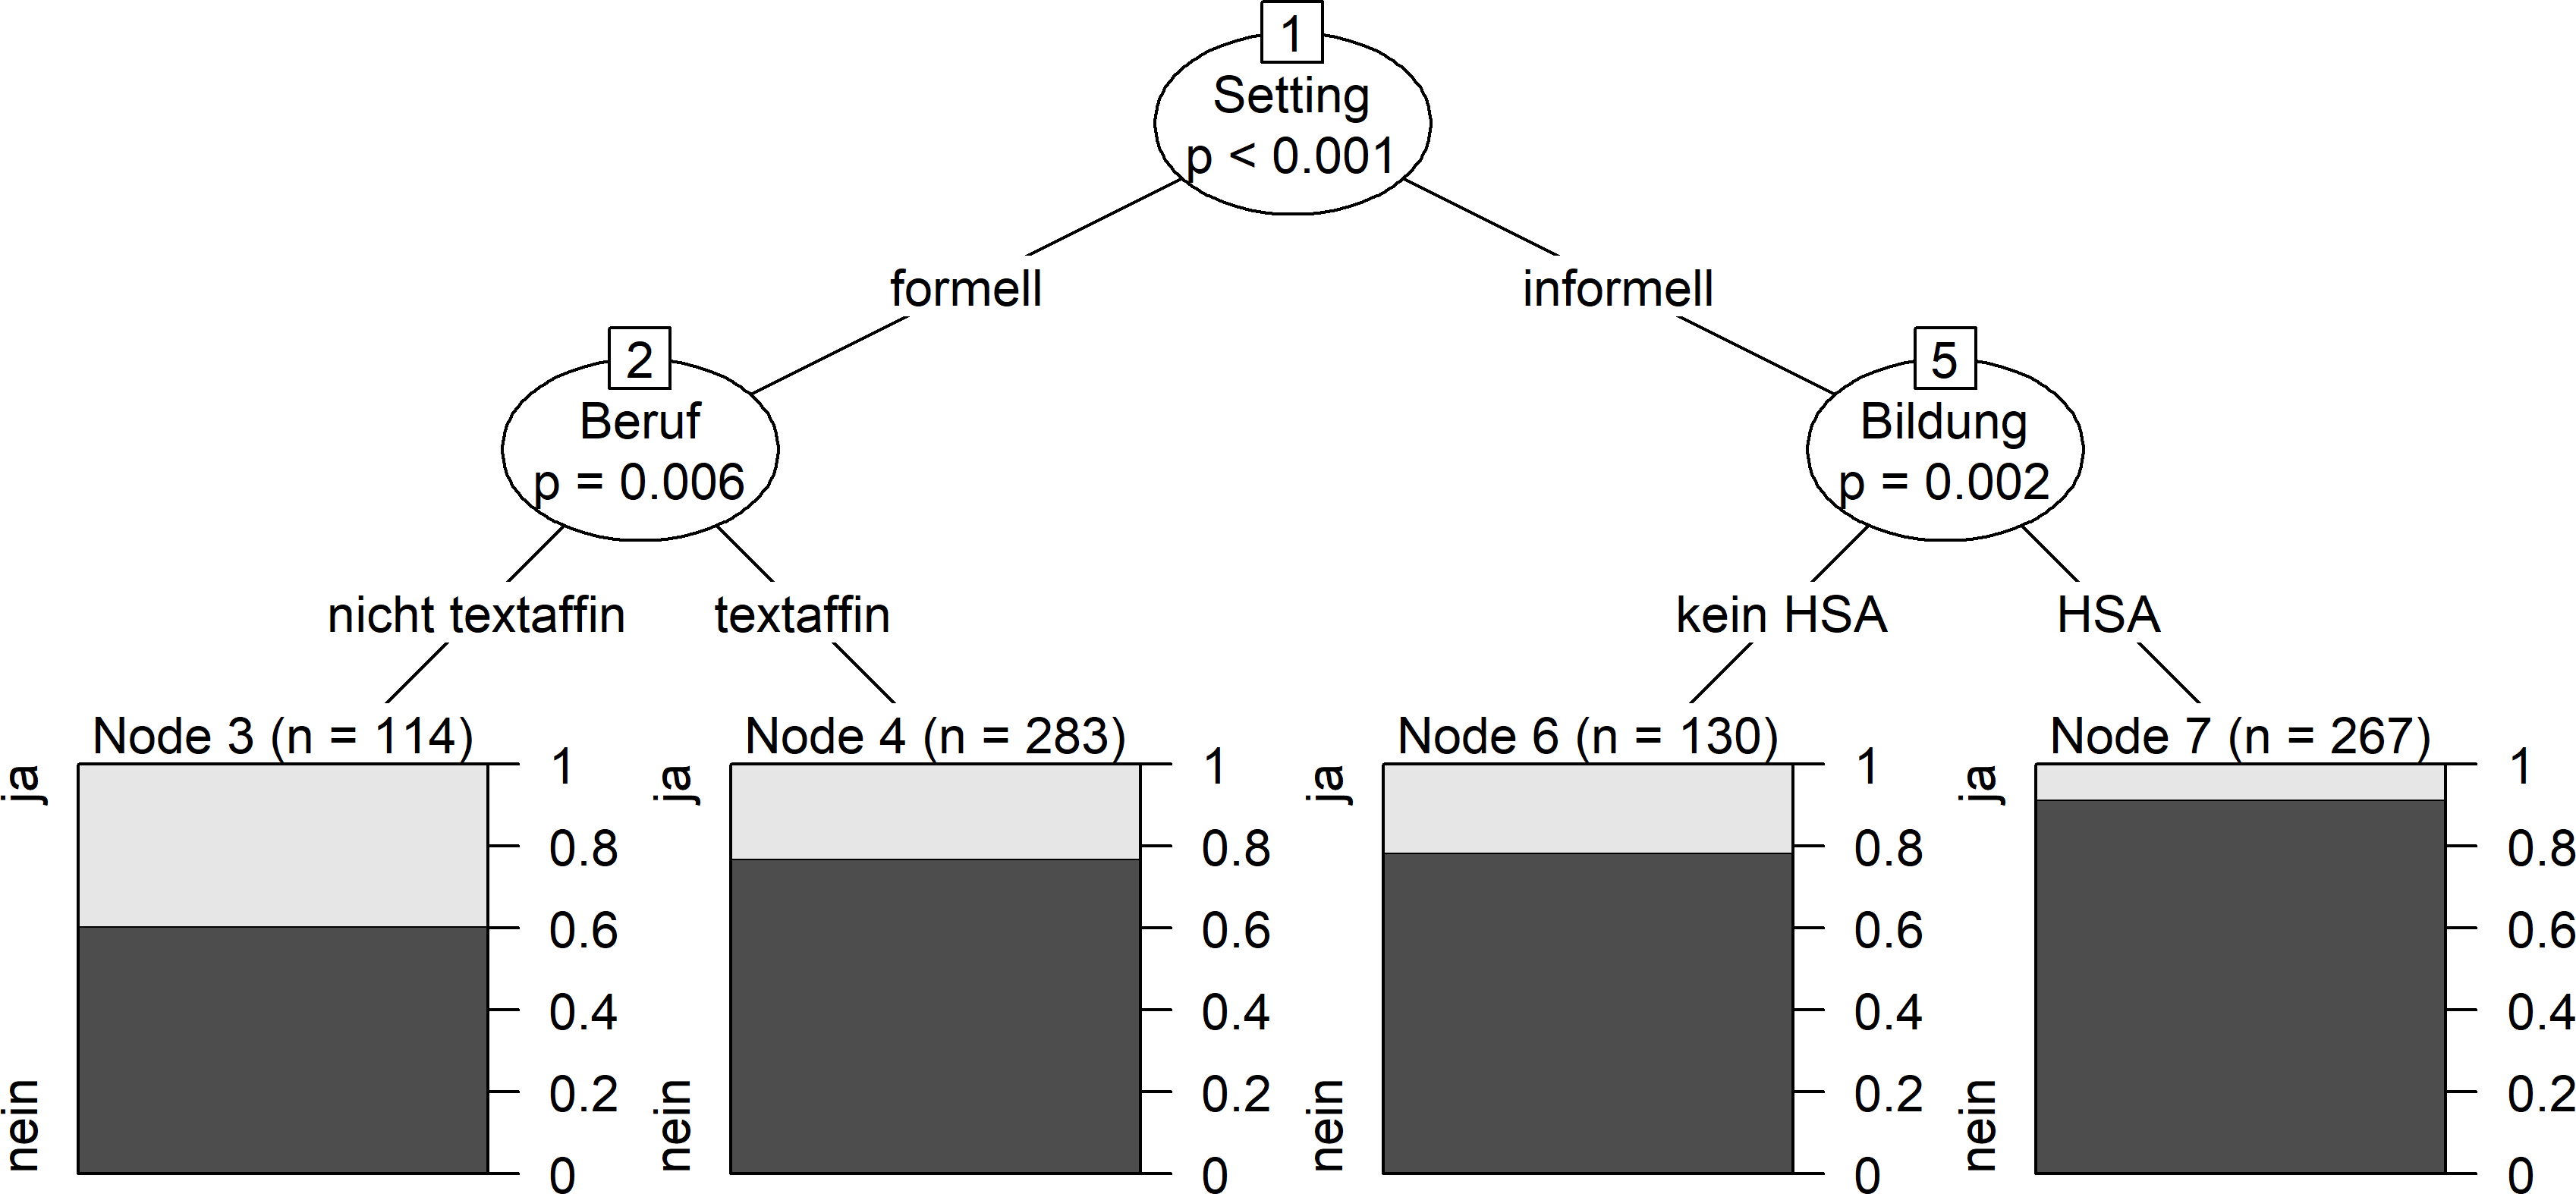
\includegraphics[angle=90, scale=0.75]{CtreeGenitivseitVerw.png}
\caption{\textit{Conditional Inference Tree} für die Angaben zur eigenen Verwendung der Genitivrektion bei \object{seit}}
\label{pic:CtreeVerwGenitivrSeit}
\end{figure}
 Die statistische Analyse der Daten aus dem Akzeptabilitätstest macht deutlich, dass die Bewertung der Dativrektion bei \wegen{} und \waehrend{} insbesondere von der Formalität des Settings und von der Herkunft der Befragten abhängt.
Auf die Angabe, ob Befragte die Variante selbst verwenden würden, hat außerdem ihre Variationstoleranz einen geringen Einfluss. 
Die Beurteilung der Genitivrektion bei \dank{} und \gegenueber{} zeigen keine Abhängigkeit von den hier getesteten Variablen.
Für die Bewertung der Korrektheit und Angemessenheit der Genitivrektion bei der Primärpräposition \object{seit} werden unterschiedliche Wahrscheinlichkeiten vorhergesagt, je nachdem, ob Befragte einen textaffinen Beruf haben.  
\subsection{Begründungen für die Unangemessenheit einer Variante}
\label{sec:Begruendungen}
% Begründungen
Bisher wurden die Antworten auf die geschlossenen Fragen im Akzeptabilitätstest ausgewertet. 
Der folgende Abschnitt widmet sich den Antworten auf die offene Frage nach dem Grund für die Einstufung als unangemessen: 
Wenn die Befragten eine Variante im Akzeptabilitätstest als unangemessen bewerteten, wurden sie mit der Frage \glqq was stört Sie?\grqq{} um eine Begründung gebeten (\autoref{sec:Akz}). 

Die Begründungen für die Ablehnung von \wegen{} oder \waehrend{} plus Dativ sowie von \dank{} oder \gegenueber{} plus Genitiv wurden analog zu den freien Assoziationen (\autoref{sec:ErgAss}) inhaltsanalytisch ausgewertet.\footnote{Begründungen für die Beurteilung des Genitivs bei der Primärpräposition \object{seit} als unangemessen wurden ebenfalls erhoben, werden aber nicht im Rahmen dieser Untersuchung ausgewertet.}
Das dafür genutzte Kategoriensystem basiert auf dem für die Assoziationen erstellten. 
Daher soll an dieser Stelle lediglich auf die Anpassungen eingegangen werden, die im Zuge des ersten Kodierungsdurchgangs an einem repräsentativen Sample der Daten erfolgt sind (zum genauen Vorgehen bei der Kategorisierung s. \autoref{sec:Akz}). 
Das Handbuch für die Kodierung der Begründungen im Akzeptabilitätstest findet sich im Anhang (\autoref{Anh:HandbuchBegr}). 
Als Kodierungseinheit diente, wie schon bei den Assoziationen, jeweils die gesamte Antwort eines/r Befragten. 
Wenn eine Antwort verschiedene Begründungen anführte, wurde sie in mehrere Kategorien einsortiert. 
%Die Schritte bei der Kategorisierung der Begründungen entsprechen denen bei der Kategorisierung der Assoziationen: 
%Nach dem ersten Kodierungsdurchgang an einem Teil der Daten wurde ein Kodierungshandbuch erstellt. 
%Anschließend wurde der komplette Datensatz zweimal in \citet{MAXQDA.19892018} kodiert, sodass die Intracoderreliabilität berechnet werden konnte.
%Ein repräsentatives Viertel der Antworten wurde auch hier zusätzlich von zwei Hilfskräften kodiert, was auch eine Kontrolle der Intercoderreliabilität zulässt. 

Für die Kodierung der Begründungen im Akzeptabilitätstest stehen insgesamt 17 Oberkategorien zur Verfügung, die sich größtenteils mit den Oberkategorien für die freien Assoziationen decken. 
Hinzugekommen sind lediglich zwei Kategorien:
Erstens die Kategorie \glqq nur Vorschlag/Benennung\grqq{} für Antworten, die keine Begründung enthalten, sondern nur auf die sprachliche Form verweisen, was zur Einstufung als unangemessen geführt hat, oder die stattdessen bevorzugte Form nennen. 
Beispiele für diese Art von Antworten sind die folgenden: 
\begin{exe}
\ex \object{Fehlender Genitiv} (Behördenangestellter, 56, zu \waehrend{} mit dem Dativ im formellen Setting)
\ex \object{Der Kasus} (Hotelrezeptionistin, 30, zu \dank{} mit dem Genitiv im formellen Setting)
\ex \object{Gegenüber dem Sachbearbeiter} (Lehramtsstudentin, 24, zu \gegenueber{} mit dem Genitiv im formellen Setting)
\end{exe}
Die zweite Oberkategorie, die hinzugekommen ist, ist die Kategorie \glqq Sprachgefühl\grqq, da es Antworten gibt, in denen Befragte ihre eigene sprachliche Intuition als Begründung für die Ablehnung einer Variante heranziehen, wie etwa hier:
\begin{exe}
\ex \object{eher während des Vortrags. Das klingt für mich besser} (Biologiedoktorandin, 25, zu \waehrend{} mit dem Dativ im formellen Setting)
\end{exe}
Da in den Begründungen aus dem Akzeptabilitätstest nie auf die Stellung einer Präposition Bezug genommen wird, fehlt die Oberkategorie \glqq Stellung\grqq{} in dem angepassten Kategorienset. 
Insgesamt stehen für die Kodierung der Begründungen für die Bewertung einer Variante als unangemessen folgende Oberkategorien zur Verfügung: \glqq Personentypus\grqq, \glqq eigener Gebrauch\grqq, \glqq Sprachgefühl\grqq, \glqq Zweifel\grqq, \glqq Formalität\grqq, \glqq Medium\grqq, \glqq Varietät\grqq, \glqq Korrektheit\grqq, \glqq Gleichgültigkeit\grqq, \glqq Ästhetik\grqq, \glqq Sprachwandel\grqq, \glqq Bedeutung und Verständlichkeit\grqq, \glqq Herleitung\grqq, \glqq nur Vorschlag/Benennung\grqq, \glqq nicht relevant\grqq, \glqq keine Angabe\grqq{} und \glqq nicht entscheidbar\grqq. 
Die Kategorie \glqq nicht relevant\grqq{} wurde für Antworten vergeben, in denen deutlich wird, dass die Unangemessenheit der Form nicht am Kasus festgemacht wird. 
Ein Beispiel dafür ist folgende Antwort: 
\begin{exe}
\ex \object{Name des Sachbearbeiters fehlt} (Chemielaborant, 27, zu \gegenueber{} mit dem Genitiv im formellen Setting)
\end{exe}
In die Kategorie \glqq keine Angabe\grqq{} fallen Antworten wie \object{nichts} oder \object{keine Ahnung}. 
\glqq Nicht entscheidbar\grqq{} wurde vergeben, wenn die Begründung unklar war, etwa bei Antworten wie \object{Grammatik} oder \object{Ausdruck}. 

Insgesamt liegen bei den Begründungen für die Unangemessenheit einer Variante deutlich weniger Antworten vor als bei den freien Assoziationen.
Dies liegt daran, dass nur diejenigen Befragten nach einer Begründung gefragt wurden, die eine Variante als unangemessen abgelehnt haben.  
In \autoref{pic:OKatBegr} ist zu sehen, wie viele Antworten in den 17 Oberkategorien jeweils kodiert wurden. 

\begin{figure}
\centering
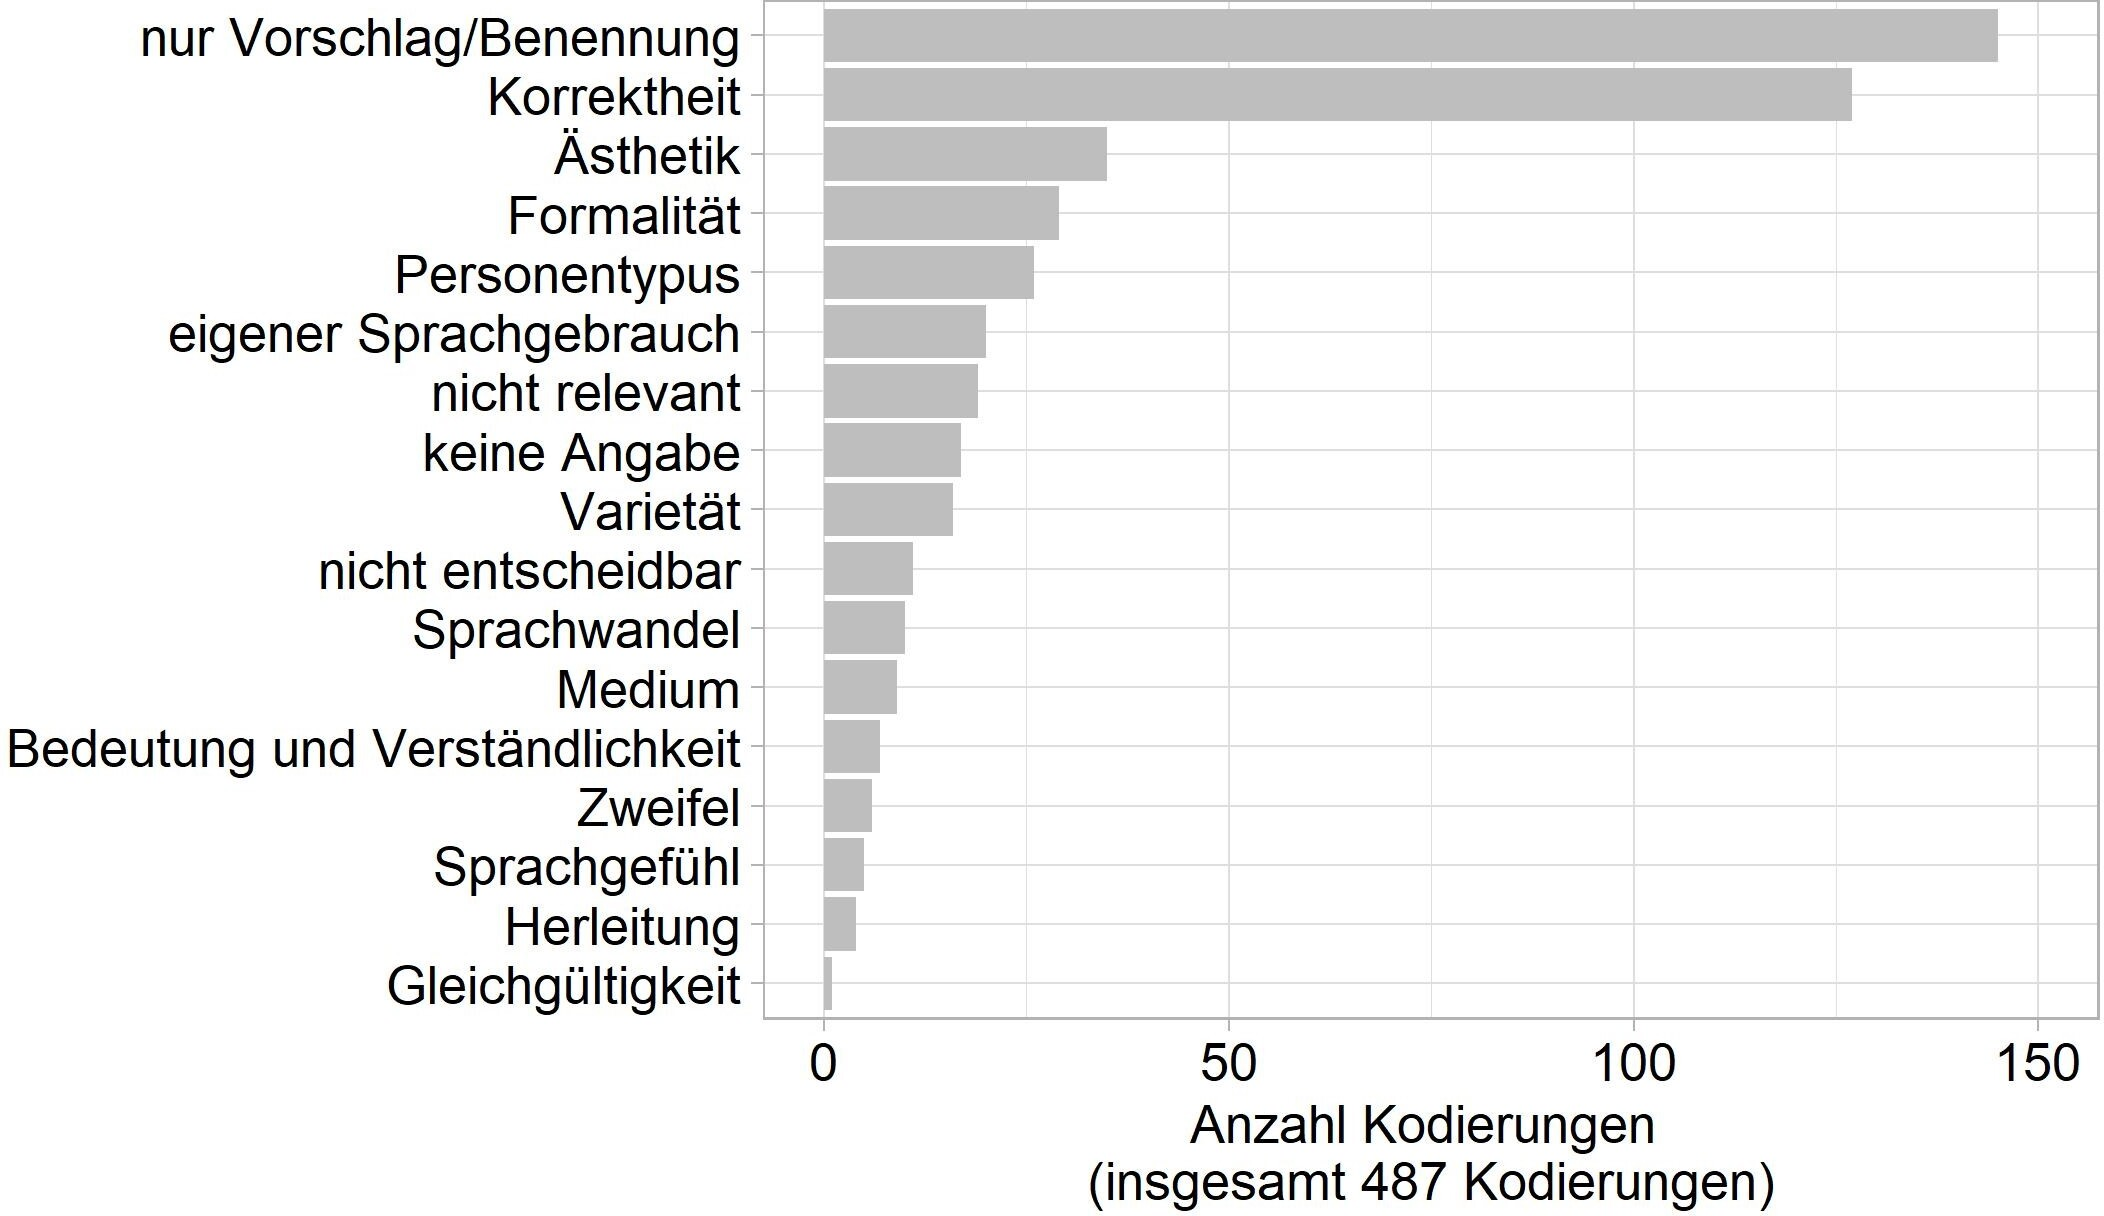
\includegraphics[width=\textwidth]{OKatBegr.jpg}
\caption{Anzahl der Kodierungen von Begründungen für die Unangemessenheit einer Variante in den Oberkategorien}
\label{pic:OKatBegr}
\end{figure}

Die Kategorie \glqq nur Vorschlag/Benennung\grqq{} ist am häufigsten vertreten:
145 Antworten enthalten lediglich einen Vorschlag oder benennen die unangemessene Form. 
Dass die meisten Befragten auf diese Art und Weise antworten, liegt an der Elizitation der Antworten durch die Frage \glqq was stört Sie?\grqq. 
Umso interessanter ist es, dass zahlreiche Befragte ihre Entscheidung auch begründen. 
Am häufigsten wird die Korrektheit bzw. Inkorrektheit einer Variante als Begründung angeführt. 
Neben \glqq nur Vorschlag/Benennung\grqq{} ist \glqq Korrektheit\grqq{} die mit Abstand häufigste Kategorie.  
127 Antworten begründen die Entscheidung im Akzeptabilitätstest über die (In)Korrektheit der Form. 
Dies zeigt, dass Angemessenheit und Korrektheit einer Variante für viele Befragte in einem engen Zusammenhang stehen. 
Die nächsthäufigen Begründungskategorien sind \glqq Ästhetik\grqq{} (35 Antworten), \glqq Formalität\grqq{} (29 Antworten) und \glqq Personentypus\grqq{} (26 Antworten). 
Alle anderen Kategorien haben höchstens 20 Vorkommnisse und scheinen damit für die Begründung, warum eine Variante als unangemessen eingestuft wurde, weniger relevant zu sein. 
Im Folgenden sollen die vier häufigsten Begründungskategorien, \glqq Korrektheit\grqq, \glqq Ästhetik\grqq, \glqq Formalität\grqq{} und \glqq Personentypus\grqq{} genauer betrachtet werden. 

%\subsection{Begründungen über Korrektheit}
Da im Akzeptabilitätstest danach gefragt wurde, was an dem Beispiel stört, wurde in den Antworten beinahe nie angemerkt, dass eine Form richtig sei. 
121 der 127 Antworten aus der Oberkategorie \glqq Korrektheit\grqq{} bezeichnen die Beispielvariante als falsch: 
\begin{exe}
\ex \object{verkehrter Fall} (Wissenschaftlicher Mitarbeiter Ingenieurwissenschaft, 26, zu \gegenueber{} mit dem Genitiv im formellen Setting) 
\ex \object{Grammatikfehler} (Geschichts- und Mathematiklehrer, 65, zu \waehrend{} mit dem Dativ im informellen Setting) 
\end{exe}
Neben solchen Beispielen, die eine Form explizit als inkorrekt benennen, wurden in \glqq Korrektheit > falsch\grqq{} auch Antworten kodiert, die dies impliziter tun, wie etwa die folgende:
\begin{exe}
\ex \object{Es heißt: während des Vortrags} (Oberstudienrat für Latein und Sport, 50, zu \waehrend{} mit dem Dativ im formellen Setting) 
\end{exe}
Indem die Genitivvariante hier mit \object{es heißt} kategorisch als richtig dargestellt wird, wird der Dativvariante die Korrektheit gleichzeitig abgesprochen. 

Die wenigen Antworten, die eine Variante als richtig bezeichnen, machen meist eine einschränkende Aussage, wie etwa diese Beispiele zeigen: 
\begin{exe}
\ex \object{Benutzt kaum jemand mehr, obwohl es noch korrekt ist} (Lehramtsstudentin, 24, zu \dank{} mit dem Genitiv im informellen Setting) \label{Bsp:BegrKorr1}
\ex \object{leider ist vermutlich beides laut Duden richtig} (Hauptschullehrer, 69, zu \wegen{} mit dem Dativ im formellen Setting) \label{Bsp:BegrKorr2}
\end{exe}
In \autoref{Bsp:BegrKorr1} wird \dank{} plus Genitiv im informellen Setting als unangemessen beurteilt. 
Die Befragte begründet diese Entscheidung damit, dass die Variante zwar richtig sei, jedoch kaum verwendet würde. 
Mit \object{mehr} und \object{noch} drückt sie zudem ihre Annahme aus, dass hier ein Sprachwandel stattfindet, bei dem die Genitivrektion zugunsten der Dativrektion weicht. 
In \autoref{Bsp:BegrKorr2} wird die Vermutung geäußert, dass der Duden bei \wegen{} sowohl die Genitiv- als auch die Dativrektion lizensiert. 
Darüber wird durch \object{leider} Bedauern ausgedrückt, wodurch deutlich wird, dass der Befragte die Dativrekion ablehnt, obwohl er davon ausgeht, dass sie laut kodifizierter Norm korrekt ist. 

\autoref{pic:BegrKorrektheit} zeigt die quantitative Verteilung der Begründungen, die auf die Korrektheit bzw. Inkorrektheit einer Variante verweisen, im Vergleich zu anderen Begründungen: 
Ein Balken bildet jeweils ab, wie häufig eine Variante insgesamt als unangemessen eingestuft wird. 
In Blautönen ist dargestellt, wie häufig diese Einstufung mit der (In-)Korrektheit der Variante begründet wird. 
Die grauen Bereiche der Balken machen sichtbar, wie häufig andere Begründungen bei einer Variante sind. 
\begin{figure}
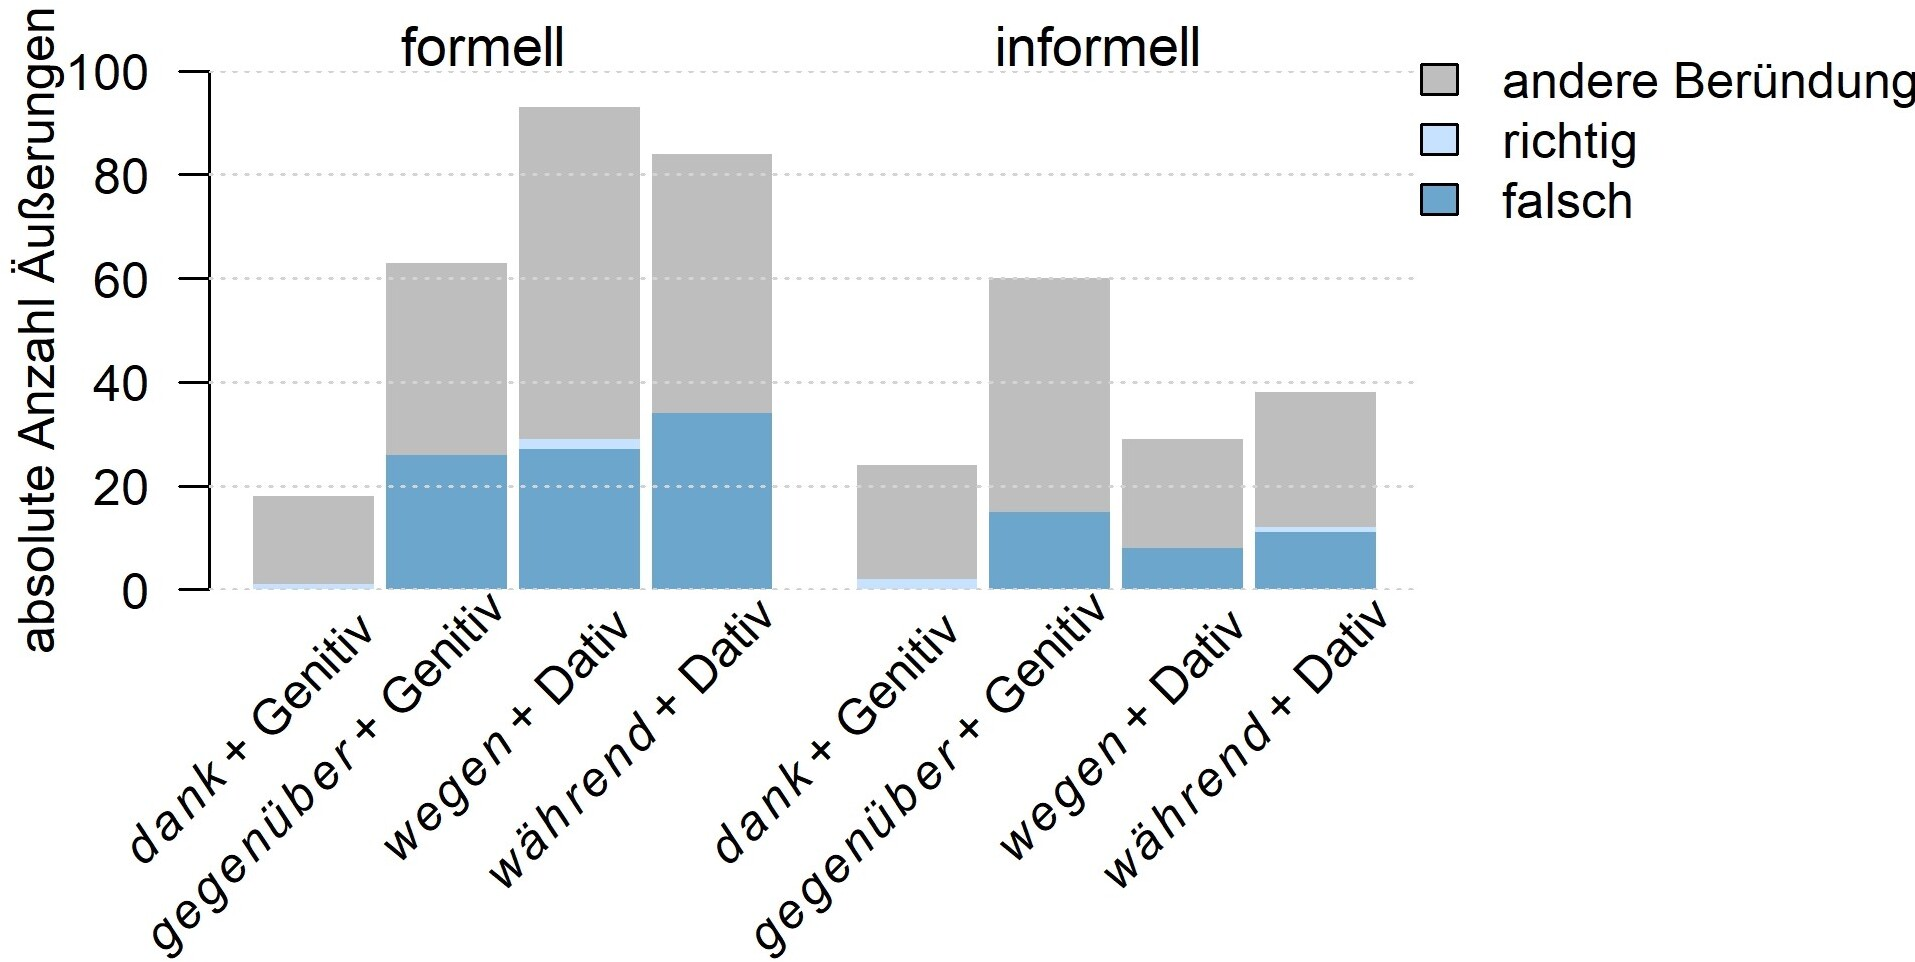
\includegraphics[width=\textwidth]{BegrKorrektheit.jpg}
\caption{Wie häufig wird die Bewertung einer Variante als unangemessen mit ihrer Inkorrektheit bzw. Korrektheit begründet?}
\label{pic:BegrKorrektheit}
\end{figure}

Im formellen Setting des Akzeptabilitätstests wird die Unangemessenheit absolut gesehen häufiger über die Inkorrektheit einer Variante erklärt als im informellen Setting, allerdings werden die Dativvarianten mit \wegen{} und \waehrend{} in diesem Setting auch insgesamt deutlich häufiger als unangemessen bewertet. 
Bei \wegen{} plus Dativ unterscheidet sich der Anteil der Begründungen, die die Inkorrektheit erwähnen, nicht zwischen den Settings und liegt jeweils bei ungefähr einem Drittel. 
Die Einstufung der Dativrektion bei \waehrend{} als unangemessen wird im formellen Teil jedoch häufiger mit Inkorrektheit begründet als im informellen (ca. 40~\% im Vergleich zu ca. 30~\%). 
Ebenso ist es bei \gegenueber{} plus Genitiv (rund 40~\% im Vergleich zu 25~\%). 
Dies könnte vermuten lassen, dass die Korrektheit dieser Formen für die Bewertung ihrer Angemessenheit in formellen Kontexten ausschlaggebender ist als in informellen, wie auch folgende Antwort nahelegt: 
\begin{exe}
\ex \object{Förmliche Briefe sollten auf korrekten Gebrauch der Grammatik achten.} (Germanistikstudent, 21, zu \gegenueber{} mit dem Genitiv im formellen Setting)
\end{exe} 
Dieser Befund lässt sich mit der engen konzeptuellen Verknüpfung von Formalität, Schriftlichkeit und Standardsprache erklären (\autoref{sec:Einheitlichkeit}). 
Ein formeller Kontext präsupponiert, dass die darin vorkommenden Varianten Teil der kodifizierten Norm sind. 
In \autoref{sec:ErgAkzallg} wurde dies bereits daran erkennbar, dass sich die Beurteilung von Korrektheit und Angemessenheit im formellen Setting nahezu deckt, während es im informellen Setting Diskrepanzen geben kann. 

Wenn \dank{} plus Genitiv als unangemessen beurteilt wird, wird dies nie damit begründet, dass diese Variante inkorrekt sei. 
Sehr häufig findet sich diese Begründungsstrategie hingegen bei \wegen{} und \waehrend{} mit dem Dativ. 
Im Gegensatz zur historisch neuen Dativrektion bei \wegen{} und \waehrend{} wird die ebenfalls historisch neue Genitivrektion bei \dank{} also bereits als korrekt angesehen. 
Dies unterstützt die in \autoref{cha:SekPraeps} diskutierte These, dass sich die neue Genitivrektion schneller durchsetzt als die neue Dativrektion \citep[s. auch][257]{Baumann2014}. 

%\subsection{Begründungen über Ästhetik}
Wird die Beurteilung einer Variante im Akzeptabilitätstest mit ästhetischen Gesichtspunkten begründet, wird die Form meist allgemein als schlecht oder unschön bezeichnet (zwölfmal).
Zehn dieser Äußerungen beziehen sich auf Dativvarianten, die anderen beiden auf die Genitivrektion bei \gegenueber. 
Letztere wird außerdem mit der Begründung abgelehnt, dass sie auffällig bzw. ungewohnt sei:
\begin{exe}
\ex \object{gegenüber dem Schaffner klingt natürlicher} (Junior Marketingmanagerin, 25, zu \gegenueber{} mit dem Genitiv im informellen Setting)
\end{exe} 
Wie bereits bei den freien Assoziationen (\autoref{sec:ErgAssAes}) zeigt sich auch bei den freien Antworten im Akzeptabilitätsteil eine klare Zuordnung der Rektionskasus zu bestimmten ästhetischen Eigenschaften. 
So wird ausschließlich die Genitivrektion mit der Begründung, gesteltzt, abgehoben oder überkorrekt zu klingen, als unangemessen eingestuft. 
Die Einbettung der im Akzeptabilitätstest präsentierten Beispiele in ein formelles und ein informelles Setting ermöglicht einen genaueren Blick auf den Zusammenhang der metapragmatischen Zuschreibungen mit dem Kontext, in dem eine Variante wahrgenommen wird. 
Wie auch im folgenden Beispiel wird die Genitivrektion nur im informellen Setting als gestelzt, abgehoben oder überkorrekt bewertet:
\begin{exe}
\ex \object{würde im Gespräch eher den Dativ verwenden, das klingt zu förmlich, zu gewollt} (Angestellte an einer Hochschule im Bereich Beratung und Information, 28, zu \dank{} mit dem Genitiv im informellen Setting) \label{Bsp:BegrForm1}
\end{exe}
Als plump oder schlampig werden hingegen fast ausschließlich Dativvarianten im formellen Setting beurteilt.\footnote{Auch \gegenueber{} plus Genitiv im informellen Setting wird einmal mit der Begründung abgelehnt, es klinge plump bzw. schlampig. } 

%\subsection{Begründungen über Formalität}
Die Antworten, die sich bei der Begründung, warum eine Variante als unangemessen eingestuft wurde, auf die Formalität beziehen, lassen sich in zwei Gruppen einteilen:
In die erste Gruppe fallen Antworten, in denen der abgefragten Rektionsvariante zugeschrieben wird, sie sei formell oder informell. 
Dazu zählt etwa die folgende Antwort zur Genitivrektion bei \dank{} im informellen Setting: 
\begin{exe}
\ex \object{hört sich zu formell an} (Medizinstudentin, 24, zu \dank{} mit dem Genitiv im informellen Setting)
\end{exe}
Die Befragte begründet ihre Ablehnung von \dank{} plus Genitiv in einem Gespräch mit einem Freund hier, indem sie die Form als formell bezeichnet. 
Die zweite Gruppe von Begründungen der Kategorie \glqq Formalität\grqq{} argumentiert hingegen damit, dass der Kontext Formalität oder Informalität erfordere:
\begin{exe}
\ex \object{umgangssprachlich evtl. tolerierbar, in förmlichen Briefen zeugt es aber von Unkenntnis} (Betriebswirt, 37, zu \wegen{} mit dem Dativ im formellen Setting)
\end{exe}
Der Dativ bei \wegen{} wird hier mit der Begründung abgelehnt, dass er in einem förmlichen Brief an ein Amt, der einen hohen Grad an Formalität erwarten lässt, einen negativen Eindruck macht.
Die der Variante zugeschriebene Wirkung (\textit{entailment}, \autoref{sec:Indexikalitaet}) wird also davon abhängig gemacht, welchen Grad an Formalität ein zuvor etablierter Kontext präsupponiert (\textit{presupposition}). 
Häufig wird in den Begründungen der Befragten sowohl auf die Formalitätsanforderungen des Kontexts als auch auf die dadurch entfaltete Wirkung der Variante Bezug genommen. 
Dies zeigt etwa das oben bereits angeführte \autoref{Bsp:BegrForm1}. 

%\subsection{Begründungen über Personentypen}
Die Begründungen der Kategorie \glqq Personentypus\grqq{} argumentieren für die Unangemessenheit einer Rektionsvariante, indem sie ihr bestimmte, meist negative Personeneigenschaften zuschreiben. 
Auffällig ist, dass die Dativrektion bei \wegen{} und \waehrend{} häufiger mit Personeneigenschaften in Verbindung gebracht wird als die Genitivrektion bei \dank{} und \gegenueber{} (20-mal zu sechsmal).
Im folgenden Beispiel etwa wird die Dativrektion bei \waehrend{} mit der Begründung abgelehnt, die Form wirke sprachlich unsicher und schlampig:
\begin{exe}
\ex \object{Die fehlende Sprachsicherheit bzw. \glqq schlampige\grqq{} Ausdrucksweise.} (Beamtin, 61, zu \waehrend{} mit dem Dativ im informellen Setting)
\end{exe}
Teilweise wird die Ablehnung der Dativrektion ganz allgemein damit begründet, sie mache einen schlechten Eindruck, wie etwa hier:
\begin{exe}
\ex \object{macht schlechten Eindruck -- Umgangssprache} (Englischlehrerin, 61, zu \wegen{} mit dem Dativ im formellen Setting)
\end{exe}
Für diese Antworten wurde im Kategoriensytem die Unterkategorie \glqq peinlich/schlechter Eindruck\grqq{} ergänzt. 
In \autoref{Bsp:BegrPersonentypus1} dagegen wird detailliert ausgeführt, wie die Verwendung von \waehrend{} plus Dativ in einem förmlichen Brief zu einem negativen Eindruck führt und welche Konsequenzen dies haben kann:
\begin{exe}
\ex \object{Unpassend; wer so schreibt, kann sich scheinbar nicht der Situation angemessen ausdrücken, kann nicht zwischen formellem und informellem Sprachgebrauch unterscheiden. Man begibt sich dadurch gegenüber dem Empfänger auf ein niedrigeres Niveau und vermittelt den Eindruck eines geringen Bildungsgrades; die Gefahr besteht, dass man dadurch weniger ernst genommen wird.} (Umweltplanungsstudent, 25, zu \waehrend{} mit dem Dativ im formellen Setting) \label{Bsp:BegrPersonentypus1}
\end{exe}
Der Gebrauch des Dativs wird hier als Mangel an Registerbewusstsein auf Seiten des/r Schreibenden gewertet: 
Da der Kontext Formalität erfordert, sollte die als formell registrierte Genitivrektion verwendet werden. 
Es wird impliziert, dass dieses Registerbewusstsein bei den EmpfängerInnen des Briefs (den MitarbeiterInnen eines Amts) vorhanden ist. 
Das fehlende Wissen um den registeradäquaten Gebrauch der Rektionsvarianten wird anschließend mit einem geringen Bildungsniveau in Verbindung gebracht. 
Schließlich wird die Vermutung geäußert, dass Personen mit niedrigeren Bildungsabschlüssen in der Interaktion mit einem Amt weniger ernst genommen werden. 

% Zusammenfassung
Die inhaltsanalytische Auswertung der freien Antworten auf die Frage \glqq was stört Sie?\grqq{} im Akzeptabilitätstest lässt sich wie folgt zusammenfassen:
Als Begründung für die Beurteilung der Dativrektion bei \wegen{} oder \waehrend{} sowie der Genitivrektion bei \gegenueber{} als unangemessen wird mit Abstand am häufigten angeführt, diese Formen seien inkorrekt. 
Des Weiteren nehmen Befragte auf die Ästhetik der Varianten Bezug, um zu begründen, warum sie sie als unangemesen eingestuft haben. 
Dabei werden die Dativvarianten meist allgemein als schlecht oder unschön bezeichnet, die Genitivrektion bei \gegenueber{} als auffällig und ungewohnt. 
In den Antworten, in denen Formalität thematisiert wird, wird zum einen damit argumentiert, dass eine Variante als formell oder informell registriert sei. 
Zum anderen wird darauf verwiesen, dass der im Akzeptabilitätstest vorgegebene Kontext einen bestimmten Formalitätsgrad erfordere. 
In den Antworten der Kategorie \glqq Personentypus\grqq{} wird den als unangemessen abgelehnten Varianten zugeschrieben, einen schlechten Eindruck zur Folge zu haben, indem VerwenderInnen der Varianten bspw. als ungebildet konzeptualisiert werden.

Der folgende Abschnitt liefert einen zusammenfassenden Überblick über alle quantitativen und qualitativen Ergebnisse des Akzeptabilitätstests. 
\subsection{Zusammenfassung der Auswertung des Akzeptabilitätstests}
\label{sec:ZsfsgAkz}
Im Akzeptabilitätsteil des Fragebogens wurden die Befragten -- aufgeteilt auf vier Gruppen -- nach ihrer Einschätzung der Korrektheit, der Angemessenheit und ihrer eigenen Verwendung von Rektionsvarianten in einem formellen und einem informellen Setting gefragt.
Abgefragt wurde die Dativrektion bei \wegen{} und \waehrend{} sowie die Genitivrektion bei \dank{}, \gegenueber{} und der Primärpräposition \object{seit}.

Von allen abgefragten Varianten wird \dank{} plus Genitiv am häufigsten als korrekt bewertet. 
In beiden Settings wird diese Form von der großen Mehrheit der Befragten akzeptiert. 
Die Dativrektion bei \wegen{} und \waehrend{} hingegen beurteilen im informellen Settings nur jeweils unter 30~\% der Befragten als korrekt, im formellen Setting sogar nur jeweils unter 20~\%. 
Obwohl \wegen{} und \waehrend{} mit der Dativrektion im \citet[915]{Duden2016} aufgeführt werden, werden diese Rektionsvarianten damit seltener als korrekt eingestuft als die in Korpora kaum belegte Genitivrektion bei \gegenueber{}. 
Auch bei \object{seit}, das als Primärpräposition laut kodifizierter Norm ausschließlich die Dativrektion zulässt, wird der Genitiv in beiden Settings von mindestens 20~\% der Befragten als korrekt angesehen. 

Als angemessen wird ebenfalls am häufigsten die Genitivrektion bei \dank{} gewertet. 
Sie gilt in beiden Settings als passend. 
Die Angemessenheit der Dativrektion bei \wegen{} oder \waehrend{} wird dagegen je nach Setting unterschiedlich bewertet:
Im formellen Setting entspricht der Anteil derer, die die Varianten als angemessen empfinden ungefähr dem Anteil derer, die sie auch als korrekt einstufen. 
Im informellen Setting jedoch erscheint die Dativrektion den Befragten deutlich häufiger angemessen als korrekt. 
Die Genitivrektion bei \gegenueber{} und \object{seit} wird jeweils ähnlich häufig als angemessen eingestuft wie sie als korrekt bewertet wird. 

Dass sie eine Variante selbst verwenden würden, geben jeweils etwas weniger Befragte an, als dass die Variante angemessen sei.
Bei \wegen{} und \waehrend{} mit dem Dativ zeigen sich auch hier Unterschiede zwischen den Settings:
In einem informellen Gespräch würde jeweils ca. die Hälfte die Dativrektion verwenden, in einem formellen Brief sind es nur jeweils unter 10~\%. 
Umgekehrt geben in Bezug auf die Genitivrektion bei \object{seit} im informellen Setting deutlich weniger Befragte an, die Variante zu verwenden als im formellen. 

Inwiefern sich die Beurteilung der Akzeptabilität in verschiedenen Befragtengruppen unterscheidet, wurde in \autoref{sec:ErgAkzNachAlter} bis \autoref{sec:ErgAkzNachVT} behandelt. 
Folgende Faktoren wurden dabei berücksichtigt:
das Alter der Befragten, ihre regionale Herkunft, ihr Bildungsstand, wie textaffin ihr Beruf ist und wie variationstolerant sie sind. 
Der Einfluss dieser Faktoren sowie der Formalität des Settings auf die Angaben zu Korrektheit, Angemessenheit und eigener Verwendung wurde anschließend mithilfe von \textit{Random Forests} statistisch überprüft. 
Dies zeigte, dass auf die Bewertung der Dativrektion bei \wegen{} oder \waehrend{} vor allem die Formalität des Settings sowie die regionale Herkunft der Befragten einen Einfluss haben. 
Bei der Beurteilung der Genitivrektion bei \dank{} und \gegenueber{} konnte keine Abhängigkeit von einem der untersuchten Faktoren festgestellt werden. 
Die Akzeptabilität der Genitivrektion mit der Primärpräposition \object{seit} scheint zu einem gewissen Grad davon abzuhängen, wie textaffin der Beruf der Befragten ist. 

Befragte, die im Akzeptabilitätstest eine Variante als unangemessen bewerteten, wurden in einer offenen Frage nach einer Begründung für diese Einschätzung gebeten. 
Die inhaltsanalytische Auswertung der Antworten macht erneut den engen Zusammenhang zwischen der Beurteilung von Korrektheit und Angemessenheit im formellen Setting deutlich:
Begründungen, die auf die Inkorrektheit der Form verwiesen, sind hier mit Abstand am häufigsten. 
Weitere Gründe, die für die Beurteilung einer Variante als unangemessen genannt werden, sind ästhetische Eigenschaften der Form sowie ihre indexikalische Verknüpfung mit negativen Personeneigenschaften und die damit verbundene Angst, einen schlechten Eindruck zu hinterlassen. 
Daneben wird für die Ablehnung als unangemessen argumentiert, indem der vom Kontext geforderte Grad an Formalität mit der Registrierung der Variante als formell oder informell abgeglichen wird. 
Der folgende Abschnitt widmet sich der Verwendung der Rektionsvarianten im Produktionsexperiment.  \section{Ergebnisse des Produktionsexperiments}
\label{sec:ErgProduktion}
Im letzten Teil des Ergebniskapitels wird das Produktionsexperiment aus dem Fragebogen ausgewertet. 
Es besteht aus zwei Lückentexten, bei denen die Befragten gebeten werden, in die Lücken nach den untersuchten Präpositionen die Form eines in Klammern angegebenen Substantivs und die Artikelform einzutragen (für eine ausführliche Beschreibung des Produktionsexperiments s. \autoref{sec:LU}):
Einer der Lückentexte ist einem klassischen Bewerbungsschreiben nachempfunden, der andere ist an eine private Textnachricht oder E-Mail angelehnt, sodass unterschiedliche Formalitätsgrade evoziert werden. 
Mit dem folgenden Beispielsatz etwa wird die Kasusrektion von \wegen{} im informellen Lückentext abgefragt:
\begin{exe}
\ex \object{Hab jetzt nochmal mit Max wegen \_\_\_\_\_\_ (Verkauf) auf dem Flohmarkt morgen telefoniert.}
\end{exe} 
Alle 397 Befragten füllten beide Lückentexte aus, sodass zu jeder Präposition in jedem Setting 397 Antworten vorhanden sind. 
Zusätzlich zu \wegen, \waehrend, \dank{} und \gegenueber{} wurde wie schon im Akzeptabilitätstest die Primärpräposition \object{seit} abgefragt. 
\autoref{table:ProdBsp} zeigt, welche Präposition mit welchen Substantiven abgefragt wurde.  
Die vollständigen Lückentexte finden sich im Fragebogen im Anhang (\autoref{Anh:Fragebogen}).
\begin{table}
\centering
\begin{tabular}{lcc}
\textit{\textbf{}} & formeller Lückentext & informeller Lückentext \\ \hline
\textit{wegen}     & \textit{Anspruch}             & \textit{Verkauf}                \\ %\hline
\textit{während}   & \textit{Studium}              & \textit{Aufbau}                 \\ %\hline
\textit{dank}      & \textit{Praktikum}            & \textit{Wetter}                 \\ %\hline
\textit{gegenüber} & \textit{Beruf}                & \textit{Plan}                   \\ %\hline
\textit{seit}      & \textit{Wegfall}              & \textit{Streit}                 \\ 
\end{tabular}
\caption{Übersicht über die Substantive, mit denen die Präpositionen im Produktionsexperiment abgefragt wurden}
\label{table:ProdBsp}
\end{table}

Im Folgenden wird überprüft, inwiefern sich die Indexikalität der Dativ- und der Genitivrektion in der Verwendung der beiden Varianten widerspiegelt. 
Die Auswertung der freien Assoziationen sowie auch die Ergebnisse des Akzeptabilitätstest haben gezeigt, dass die Rektionsvarianten metapragmatisch mit Kategorien wie (In)Korrektheit, (In)Formalität, Standardsprache, Regionalsprache, Sprachwandel und mit verschiedenen Personentypen verknüpft sind. 
Wie diese mit der Kasuswahl in den Lückentexten zusammenhängen, wird im Folgenden näher beleuchtet. 

% Änderung Anfang!
Um sicherzugehen, dass die als unterschiedlich formell konzipierten Lückentext von Befragten auch so eingeschätzt werden, wurde die Wahrnehmung der Formalität beider Texte in einer zusätzlichen Umfrage überprüft. 
Auf diese Überprüfung wird in \autoref{sec:FormLU} eingegangen. 
% Änderung Ende!
Sowohl die Auswertung der freien Assoziationen als auch die Ergebnisse des Akzeptabilitätstests unterstreichen, wie relevant die Formalität des Kontexts ist. Daher wird in \autoref{sec:ErgProdInfForm} die Kasuswahl im formellen Lückentext mit der Kasuswahl im informellen Lückentext verglichen. 
Anschließend werden unterschiedliche Befragtengruppen in den Blick genommen, die indexikalisch mit einem bestimmten Kasusgebrauch verknüpft sind:
In \autoref{sec:ErgProdNachAlter} wird untersucht, wie das Alter der Befragten mit ihrer Kasuswahl zusammenhängt.
Dies ist relevant, da die Kategorie \glqq Alter\grqq{} über die Konzeptualisierung als Sprachwandelphänomen mit der Rektionsvariation indexikalisch verknüpft ist. 
Da die Rektionsvarianten sich in ihrer Verortung in Regional- und Standardsprache unterscheiden, wird in \autoref{sec:ErgProdNachHerkunft} die Kasuswahl nord- und süddeutscher Befragter verglichen. 
\autoref{sec:ErgProdNachBildung} und \autoref{sec:ErgProdNachSk} nehmen einen Vergleich der Kasuswahl nach dem Bildungsstand der Befragten und nach der Textaffinität ihres Berufs vor und richten den Blick damit auf die {Ka\-te\-gorien} \glqq Bildung\grqq{} und \glqq Sprachkompetenz\grqq.
Schließlich geht es in \autoref{sec:ErgProdNachVT} um die Abhängigkeit der Kasuswahl von der Variationstoleranz, die als Indikator dafür gewertet werden kann, wie stark sich Befragte der Standardsprachideologie verschreiben. 

Der Einfluss der in \autoref{sec:ErgProdInfForm} bis \autoref{sec:ErgProdNachVT} dargestellten Faktoren auf die Kasuswahl bei \wegen, \waehrend, \dank, \gegenueber{} und der Primärpräposition \object{seit} wird mithilfe von \textit{Conditional Inference Trees} und \textit{Random Forests} statistisch überprüft (\autoref{sec:ErgProdCTrees}). 
\autoref{sec:ErgProdZusammenfassung} bietet eine Zusammenfassung der Ergebnisse aus dem Produktionsexperiment. 
%Änderung Anfang!
\subsection{Wahrgenommene Formalität der Lückentexte}
\label{sec:FormLU}
In einer zusätzlichen Umfrage wurde überprüft, inwiefern die beiden Lückentexte von SprachbenutzerInnen als unterschiedlich formell wahrgenommen werden. 
Hierfür wurden die Texte nicht als Lückentexte präsentiert, sondern die Präpositionen \textit{wegen}, \textit{während}, \textit{dank}, \textit{gegenüber} und \textit{seit} erschienen entweder alle mit dem Genitiv oder alle mit dem Dativ. 
Insgesamt wurden 63 Personen\footnote{Das Durchschnittsalter liegt bei 35 Jahren, 45 Personen sind weiblich, 16 männlich, eine Person ordnet sich einem anderen Geschlecht zu und eine Person möchte keine Angabe zu ihrem Geschlecht machen. Regional sind die Befragten über ganz Deutschland verteilt.} über SoSciSurvey \citep{Leiner.2014} befragt.
Sie wurden per Zufallsgenerator auf vier Gruppen aufgeteilt: 
\begin{enumerate}
\item Formell gestalteter Lückentext (Bewerbungsschreiben) mit Dativrektion bei allen Präpositionen
\item Formell gestalteter Lückentext (Bewerbungsschreiben) mit Genitivrektion bei allen Präpositionen 
\item Informell gestalteter Lückentext (private Textnachricht) mit Dativrektion bei allen Präpositionen
\item Informell gestalteter Lückentext (private Textnachricht) mit Genitivrektion bei allen Präpositionen
\end{enumerate}
\autoref{pic:WahrnFormLu} zeigt, wie formell die einzelnen Texte von den Befragten wahrgenommen werden. 
\begin{figure}
\centering
\includegraphics[width=\textwidth]{WahrnFormLu}
\caption{Wahrnehmung der Formalität der Lückentexte}
\label{pic:WahrnFormLu}
\end{figure}

Der einem Bewerbungsschreiben nachempfundene Text mit Dativrektion bei allen Präpositionen wird von fünf Befragten als formell und von sechs Befragten als eher formell eingestuft.\footnote{Im Fragebogen waren die Zwischenstufen bewusst nicht beschriftet. Bezeichnungen wie \glqq eher formell\grqq{} werden hier lediglich genutzt, um die einzelnen Stufen zu benennen.} 
Zwei Personen wählten den mittleren Skalenpunkt, konnten sich also nicht zwischen formell und informell entscheiden. Eine Person gibt an, den Text als eher informell wahrzunehmen. 
Wird Befragten der gleiche Text mit der Genitivrektion bei allen Präpositionen vorgelegt, sieht die Verteilung ähnlich aus. 
Hier entscheiden sich insgesamt 15 Personen für formell bzw. eher formell, eine Person empfindet den Text als eher informell. 

Der zweite Text, der durch Mündlichkeits- und Informalitätsmarker an eine private Textnachricht erinnern soll, wird von dern Befragten als deutlich informeller wahrgenommen. 
Bei der Version mit Dativrektion geben 13 Personen an, den Text als informell wahrzunehmen, fünf Befragte geben durch Auswahl der angrenzenden Skalenstufe an, dass sie den Text als eher formell wahrnehmen. 
Eine Person entscheidet sich für die mittlere Skalenstufe und eine weitere Person nimmt den Text als eher formell wahr. 
Der gleiche Text mit Genitivrektion wird von acht Befragten als informell und von vier als eher informell empfunden.
Eine Person wählt die mittlere Skalenstufe. 

Insgesamt zeigt die Überprüfung der wahrgenommenen Formalität der Texte, dass diese jeweils geeignet sind, um als Lückentexte unterschiedliche Formalitätsgrade zu evozieren. 
 
% Änderung Ende! 

\subsection{Kasuswahl im formellen und im informellen Lückentext}
\label{sec:ErgProdInfForm}
% Kasuswahl nach Register
Für die Auswertung der Lückentexte wurden alle Textfeldeingaben, die eindeutig als Genitivform erkennbar sind, zusammengefasst (etwa \object{des Plans} und \object{des Planes}) sowie alle Eingaben, die eindeutig als Dativform erkennbar sind (etwa \object{dem Plan} und \object{Dem Plan}).\footnote{Dem Genitiv wurde auch die Pluralform \object{der Verkäufe} zugerechnet.} 
Neben den als Dativ oder Genitiv klassifizierten Antworten gibt es außerdem Antworten, die keinem der beiden Kasus zugeordnet werden konnten (etwa \object{dem Verkaufs}). 
Diese wurden in der Kategorie \glqq Sonstiges\grqq{} zusammengefasst. 
Im Folgenden wird zunächst die Kasuswahl bei den Sekundärpräpositionen besprochen, anschließend die Wahl bei der Primärpräposition \object{seit}.

\autoref{pic:KasuswahlNachRegister} zeigt für alle vier Sekundärpräpositionen, wie häufig prozentual Genitiv- und Dativformen sowie sonstige Formen im formellen und im informellen Lückentext gewählt wurden. 
Das augenfälligste Ergebnis ist, dass die Genitivrektion bei allen Präpositionen bis auf \gegenueber{} insgesamt deutlich überwiegt.
Sowohl bei den ursprünglichen Genitivpräpositionen \wegen{} und \waehrend{} als auch bei der ursprünglichen Dativpräposition \dank{} wurde der Genitiv im formellen und im informellen Lückentext häufiger gewählt als der Dativ (für die genauen Zahlen s. auch \autoref{table:AnhProd} im Anhang). 
Bei \wegen{} und \waehrend{} im informellen Text ist dieses Ergebnis vor dem Hintergrund der Angaben im Akzeptabilitätstest zunächst überraschend: 
Die Mehrheit der Befragten empfindet die Dativrektion bei diesen Präpositionen in einem informellen Gespräch als angemessen und ungefähr die Hälfte gibt an, den Dativ selbst zu verwenden (\autoref{sec:ErgAkzallg}). 
Für die Verwendung scheint jedoch eher die Einschätzung als korrekt enscheidend zu sein: 
Der Anteil der Dativrektion im Produktionsexperiment entspricht ungefähr dem Anteil der Bewertung dieser Variante als korrekt. 
Bei \gegenueber{} verwenden dagegen die allermeisten Befragten in beiden Lückentexten die Dativrektion (jeweils knapp 90~\%).
Hier ist der Anteil derer, die den Genitiv setzen, also deutlich geringer als der Anteil derer, die diesen Kasus im Akzeptabilitätstest als korrekt oder angemessen bewerten (\autoref{sec:ErgAkzallg}). 
\begin{figure}
\centering
\includegraphics[width=\textwidth]{KasuswahlNachRegister}
\caption{Ergebnisse des Produktionsexperiments}
\label{pic:KasuswahlNachRegister}
\end{figure}

Obwohl insgesamt der Genitiv also klar bevorzugt wird, ist in den Daten ein deutlicher Unterschied zwischen dem formellen und dem informellen Lückentext erkennbar.
Die Dativrektion ist im informellen Teil des Produktionsexperiments weitaus häufiger.
Bei \wegen{} wählen im formellen Teil rund 87~\% der Befragten den Genitiv, im informellen Teil hingegen nur ca. 70~\%. 
\object{Während} wird im formellen Lückentext von ungefähr 94~\% mit dem Genitiv verwendet, im informellen Lückentext jedoch nur von ungefähr 81~\%. 
Bei \dank{} entscheiden sich ca. 92~\% im formellen Teil für den Genitiv und rund 82~\% im informellen Teil. 
Lediglich bei \gegenueber{} ist kein nennenswerter Unterschied erkennbar (ca. 8~\% Genitivrektion im formellen Lückentext und ca. 9~\% im informellen). 

Dass die Genitivrektion bei \wegen, \waehrend{} und \dank{} insgesamt so stark überwiegt, kann auf die Wirkung der Indexikalität zurückgeführt werden: 
Indem sie im Produktionsexperiment die Genitivrektion nutzen, inszenieren sich Befragte als gebildet, professionell und kompetent. 
Damit positionieren sie sich gegenüber der Forscherin und der Institution, der sie angehört. 
Dabei spielte wahrscheinlich auch eine Rolle, dass die Befragung von einigen als Testsituation empfunden wurde, wie Kommentare von Befragten deutlich machen:  
\begin{exe}
\ex \object{gibt es ein Lösungsblatt? Je mehr man darüber nachdenkt, desto unsicherer wird man...} (Sonderpädagogikstudent, 24) \label{Bsp:Loesungsblatt}
\ex \object{Auflösung der Textbeispiele wäre noch interessant gewesen} (keine Berufsangabe, männlich, 37) \label{Bsp:Aufloesung}
\ex \object{Im Test war ich bei der Aufgabe mit der Bewerbung teilweise mit dem englischen Fachjargon überfordert, bzw. ich kannte dort einige Begriffe nicht.} (keine Berufsangabe, weiblich, 32) \label{Bsp:Test}
\end{exe}
In einer solchen Testsituation könnte der Genitiv angemessener erscheinen, da er als standardsprachlich und daher korrekt gilt (s. Ergebnisse in \autoref{sec:ErgAssKorrektheit} und \autoref{sec:ErgAssFormMedVar}). 
Der Befragte, von dem der Kommentar in \autoref{Bsp:Loesungsblatt} stammt, verwendet im Produktionsexperiment immer den Genitiv, außer im Fall von \object{seit} im formellen Lückentext. 
Bei den Befragten, von denen die beiden anderen Kommentare stammen, lässt sich eine solch starke Tendenz zum Genitiv jedoch nicht erkennen.\footnote{Der Befragte aus \autoref{Bsp:Aufloesung} verwendet in beiden Lückentexten bei \wegen{}, \waehrend{} und \dank{} den Genitiv, bei \gegenueber{} und \object{seit} den Dativ. Die Befragte aus \autoref{Bsp:Test} verwendet im formellen Teil ebenfalls \wegen{}, \waehrend{} und \dank{} mit dem Genitiv, im informellen jedoch nur \wegen{} und \waehrend{}.}

Berücksichtigt man, dass die Befragten sich einer Sprachautorität gegenübersehen, die scheinbar ihr sprachliches Können testet, sind die Unterschiede zwischen dem formellen und dem informellen Lückentext umso bemerkenswerter. 
Es ist zu vermuten, dass der Genitiv in natürlichen informellen Interaktionssituationen seltener gebraucht wird und Formalität und Kasuswahl daher im natürlichen Sprachgebrauch noch sehr viel stärker interagieren. 
%GLMM berichten 
%Diese Ergebnisse deuten darauf hin, dass die Verweiskraft der Varianten einen Einfluss auf die Verwendung hat: Der Dativ gilt eher in informellen Kontexten als angemessen, Genitiv in formellen.
% korreliert häufiger Genitivgebrauch im formellen Setting mit häufigem Genitivgebrauch im informellen Setting?

\autoref{pic:KasuswahlSeit} zeigt die Kasuswahl bei der Primärpräposition \object{seit} im Produktionsexperiment. 
Wie bei Primärpräpositionen zu erwarten, überwiegt die Dativrektion deutlich. 
Allerdings entscheiden sich im formellen Lückentext immerhin ca. 11~\% der Befragten für die Genitivrektion (s. auch \autoref{table:AnhProd} im Anhang). 
\object{Seit} wird im formellen Teil also sogar etwas häufiger mit dem Genitiv verwendet als \gegenueber. 
Im informellen Teil wählen nur ca. 6~\% den Genitiv mit \object{seit}. 
Auch bei der Primärpräposition, die eigentlich keine Kasusschwankung aufweist, ist also trotz des insgesamt eher formellen Settings der Befragung ein Zusammenhang zwischen der Kasuswahl der Befragten und dem Register erkennbar. 
In beiden Settings ist die Zahl der Befragten, die die Genitivrektion bei \object{seit} verwenden, niedriger als die Zahl derer, die sie im Akzeptabilitätstest als korrekt oder angemessen bewerten (\autoref{sec:ErgAkzallg}). 
\begin{figure}
\centering
\includegraphics[width=\textwidth]{KasuswahlNachRegisterSeit.jpg}
\caption{Kasuswahl im Produktionsexperiment bei der Primärpräposition \object{seit}}
\label{pic:KasuswahlSeit}
\end{figure}

Wie in \autoref{sec:ErgAkzallg} erwähnt, könnte die Möglichkeit der kausalen Interpretation von \object{seit} die Wahl des Genitivs begünstigen. 
Im formellen Lückentext lautet der Satz, mit dem die Rektion von \object{seit} abgefragt wird, \object{seit \_\_\_\_\_ (Wegfall) einer Stelle war ich sogar für die Organisation eines Weiterbildungsworkshops zuständig}.
Der Satz im informellen Lückentext ist \object{seit \_\_\_\_\_ (Streit) neulich hab ich nix mehr von ihm gehört}.
Beide Sätze lassen neben einer temporalen auch eine kausale Lesart zu, da diese beiden Konzepte metonymisch miteinander verknüpft sind \citep[s.][]{Traugott.1991}. 
%Im Falle des ersten kann sogar davon ausgegangen werden, dass diese Lesart dominiert: 
%Die Präpositionalphrase liefert hier die Erklärung dafür, warum die Verfasserin des Bewerbungsschreibens als Werkstudentin eine so verantwortungsvolle Aufgabe wie die Organisation eines Weiterbildungsworkshops innehatte.
%Im Falle des Satzes aus dem informellen Lückentext sind die temporale und die kausale Lesart gleichermaßen plausibel, da hier die Möglichkeit offengehalten wird, dass der erwähnte Freund sich aus einem anderen Grund nicht gemeldet hat. 
%Der häufigere Gebrauch der Genitivrektion mit \object{seit} im formellen Lückentext könnte also auch in der stärker kausalen Lesart der Präpositionalphrase begründet sein. 

An den Ergebnissen des Produktionsexperiments wird deutlich, dass der Grad der Formalität, der in einem Kontext bereits etabliert ist, einen Einfluss auf die Wahl der Rektionsvariante bei \wegen{}, \waehrend{} und \dank{} hat: 
Die Dativrektion gilt eher in informellen Kontexten als angemessen, die Genitivrektion in formellen. 
Diese Registerunterschiede zeigen sich trotz einer generellen 
Tendenz zum Genitiv, die sich wahrscheinlich mit der Befragungssituation erklären lässt, in der sich Befragte als gebildet und sprachkompetent positionieren möchten.
In den folgenden Abschnitten wird untersucht, welche weiteren Faktoren eine Rolle bei der Kasuswahl spielen. 
\subsection{Kasuswahl und Alter}
\label{sec:ErgProdNachAlter}
Wie bereits für die Akzeptabilität (\autoref{sec:ErgAkzNachAlter}) soll auch für die Produktion untersucht werden, ob die älteste Befragtengruppe (61--85 Jahre) sich von der jüngsten Befragtengruppe (18--25) unterscheidet. 
Die Kategorie \glqq Alter\grqq{} ist deswegen von Interesse, weil die Rektionsschwankung der Sekundärpräpositionen als Sprachwandelphänomen konzeptualisiert wird: 
Wie in \autoref{sec:ErgAssSprachwandel} beschrieben, gehen Befragte dabei meist davon aus, dass die Genitivrektion die ältere Variante sei.
In den freien Assoziationen werden die Beispiele zwar nur selten explizit älteren Personen zugeschrieben (\autoref{sec:ErgAssPersonen}), allerdings werden sie mit Eigenschaften in Verbindung gebracht, die in der Gesellschaft häufig als typisch für ältere Menschen gelten. 
So nennen Befragte die Genitivvarianten im Fragebogen etwa streng, seriös und altmodisch.  
Der sozialsymbolische Verweis auf die Kategorie \glqq Alter\grqq{} ist also nicht auf der ersten, sondern auf der zweiten oder dritten indexikalischen Ordnung angesiedelt (\autoref{sec:Indexikalitaet}). 

Um zu überprüfen, ob sich verschiedene Altersguppen in ihrem Gebrauch der Genitiv- und Dativrektion tatsächlich unterscheiden, wird die Kasuswahl der 18- bis 25-Jährigen im Produktionsexperiment mit derjenigen der 61- bis 85-Jährigen verglichen. 
Anders als bei den Ergebnissen des Akzeptabilitätsteils werden die vier Sekundärpräpositionen \wegen, \waehrend, \dank{} und \gegenueber{} sowie die Primärpräposition \object{seit} hier einzeln betrachtet, da im Produktionsexperiment alle 397 Befragten alle Lücken bearbeiteten. 
Die Altersgruppe 18 bis 25 umfasst 104 Befragte, die Altersgruppe 61 bis 85 nur 47. 
Beim Vergleich der beiden Gruppen ist zu berücksichtigen, dass unter den älteren Befragten besonders viele Personen aus Norddeutschland sowie besonders viele Personen ohne Abitur sind (\autoref{sec:HerkunftundDialekt} und \autoref{sec:Bildung}). 
Aufgrund der geringen Anzahl der Befragten in der höheren Altersgruppe dienen die Prozentangaben im Folgenden lediglich zur besseren Orientierung beim Vergleich zwischen den Gruppen und sind allein nicht aussagekräftig. 

\autoref{table:ErgProdWegenNachAlter} zeigt die Kasuswahl bei \wegen{} in der Gruppe der 18- bis 25-Jährigen sowie in der Gruppe der 61- bis 85-Jährigen.
Im formellen Lückentext wird \wegen{} von den jüngeren Befragten kaum anders verwendet als von den älteren Befragten. 
Von den jüngeren BefragungsteilnehmerInnen entscheiden sich hier rund 10~\% für den Dativ, von den älteren ca. 11~\% (fünf Personen). 
Leichte Unterschiede zwischen den Gruppen zeigen sich im informellen Teil des Produktionsexperiments:
Hier setzen ca. 29~\% der 18- bis 25-Jährigen den Dativ, aber nur ungefähr 23~\% (elf Personen) der 61- bis 85-Jährigen. 
Die Jüngeren scheinen ihre Kasuswahl also etwas stärker von der Formalität des Settings abhängig zu machen. 
% Please add the following required packages to your document preamble:
% \usepackage{multirow}
\begin{table}
\centering
\begin{tabular}{llrr|rr}
\multicolumn{6}{l}{\textit{\textbf{wegen}}}                                                                                                                                                                                                                     \\ \hline
                                                                                  &           & \multicolumn{2}{c}{\begin{tabular}[c]{@{}c@{}}\textbf{18--25 Jahre}\\ (n=104)\end{tabular}} & \multicolumn{2}{|c}{\begin{tabular}[c]{@{}c@{}}\textbf{61--85 Jahre}\\ (n=47)\end{tabular}} \\ \hline
\multirow{3}{*}{\begin{tabular}[c]{@{}l@{}}formeller \\ Lückentext\end{tabular}}  & Dativ     & 10                                  & (9,62 \%)                                  & 5                                   & (10,64 \%)                                 \\ %\cline{2-6} 
                                                                                  & Genitiv   & 94                                  & (90,38 \%)                                 & 41                                  & (87,23 \%)                                 \\ %\cline{2-6} 
                                                                                  & Sonstiges  & 0                                   & (0 \%)                                     & 1                                   & (2,13 \%)                                  \\ \hline
\textbf{}                                                                         & \textbf{} & \multicolumn{2}{c}{\begin{tabular}[c]{@{}c@{}}\textbf{18--25 Jahre}\\ (n=104)\end{tabular}} & \multicolumn{2}{|c}{\begin{tabular}[c]{@{}c@{}}\textbf{61--85 Jahre}\\ (n=47)\end{tabular}} \\ \hline
\multirow{3}{*}{\begin{tabular}[c]{@{}l@{}}informeller\\ Lückentext\end{tabular}} & Dativ     & 30                                  & (28,85 \%)                                 & 11                                  & (23,4 \%)                                  \\ %\cline{2-6} 
                                                                                  & Genitiv   & 72                                  & (69,23 \%)                                 & 35                                  & (74,47 \%)                                 \\ %\cline{2-6} 
                                                                                  & Sonstiges  & 2                                   & (1,92 \%)                                  & 1                                   & (2,13 \%)                                  \\ \hline
\end{tabular}
\caption{Kasuswahl bei \wegen{} im formellen und im informellen Lückentext nach Altersgruppen}
\label{table:ErgProdWegenNachAlter}
\end{table}

Auch bei der Präposition \waehrend{} verhalten sich jüngere und ältere Befragte im formellen Lückentext untereinander sehr ähnlich (s. \autoref{table:ErgProdWaehrendNachAlter}). 
Nur ca. 5 bzw. 4~\% setzen den Dativ.
Im informellen Teil zeigen sich bei \waehrend{} aber deutliche Unterschiede:
Ungefähr 22~\% der 18- bis 25-Jährigen entscheiden sich hier für die Dativrektion, unter den 61- bis 85-Jährigen sind es jedoch gerade einmal ca. 2~\%, was bei der geringen Gruppengröße einer einzigen Person entspricht. 
Die Unterschiede zwischen den Altersgruppen im informellen Lückentext sind bei \waehrend{} also größer als bei \wegen, d.\,h., die Kontextsensitivität der Jüngeren zeigt sich hier noch stärker. 
% Please add the following required packages to your document preamble:
% \usepackage{multirow}
% \usepackage[table,xcdraw]{xcolor}
% If you use beamer only pass "xcolor=table" option, i.e. \documentclass[xcolor=table]{beamer}
\begin{table}
\centering
\begin{tabular}{llrr|rr}
\multicolumn{6}{l}{\textit{\textbf{während}}}                                                                                                                                                                                                                         \\ \hline
                                                                                   &           & \multicolumn{2}{c}{\begin{tabular}[c]{@{}c@{}}\textbf{18--25 Jahre}\\ (n=104)\end{tabular}} & \multicolumn{2}{|c}{\begin{tabular}[c]{@{}c@{}}\textbf{61--85 Jahre}\\ (n=47)\end{tabular}} \\ \hline
                                                                                   & Dativ     & {\color[HTML]{000000} 5}             & {\color[HTML]{000000} (4,81 \%)}             & {\color[HTML]{000000} 2}             & {\color[HTML]{000000} (4,26 \%)}            \\ %\cline{2-6} 
                                                                                   & Genitiv   & {\color[HTML]{000000} 99}            & {\color[HTML]{000000} (95,19 \%)}            & {\color[HTML]{000000} 44}            & {\color[HTML]{000000} (93,62 \%)}           \\ %\cline{2-6} 
\multirow{-3}{*}{\begin{tabular}[c]{@{}l@{}}formeller \\ Lückentext\end{tabular}}  & Sonstiges  & {\color[HTML]{000000} 0}             & {\color[HTML]{000000} (0 \%)}                & {\color[HTML]{000000} 1}             & {\color[HTML]{000000} (2,13 \%)}            \\ \hline
\textbf{}                                                                          & \textbf{} & \multicolumn{2}{c}{\begin{tabular}[c]{@{}c@{}}\textbf{18--25 Jahre}\\ (n=104)\end{tabular}} & \multicolumn{2}{|c}{\begin{tabular}[c]{@{}c@{}}\textbf{61--85 Jahre}\\ (n=47)\end{tabular}} \\ \hline
                                                                                   & Dativ     & {\color[HTML]{000000} 23}            & {\color[HTML]{000000} (22,12 \%)}            & {\color[HTML]{000000} 1}             & {\color[HTML]{000000} (2,13 \%)}            \\ %\cline{2-6} 
                                                                                   & Genitiv   & {\color[HTML]{000000} 81}            & {\color[HTML]{000000} (77,88 \%)}            & {\color[HTML]{000000} 45}            & {\color[HTML]{000000} (95,74 \%)}           \\ %\cline{2-6} 
\multirow{-3}{*}{\begin{tabular}[c]{@{}l@{}}informeller\\ Lückentext\end{tabular}} & Sonstiges  & {\color[HTML]{000000} 0}             & {\color[HTML]{000000} (0 \%)}                & {\color[HTML]{000000} 1}             & {\color[HTML]{000000} (2,13 \%)}            \\ \hline
\end{tabular}
\caption{Kasuswahl bei \waehrend{} im formellen und im informellen Lückentext nach Altersgruppen}
\label{table:ErgProdWaehrendNachAlter}
\end{table}

Wie bereits bei den beiden ursprünglichen Genitivpräpositionen \wegen{} und \waehrend{} gibt es auch bei der ursprünglichen Dativpräposition \dank{} im formellen Teil des Produktionsexperiments kaum Unterschiede zwischen den beiden Altersgruppen (s. \autoref{table:ErgProdDankNachAlter}). 
% Please add the following required packages to your document preamble:
% \usepackage{multirow}
\begin{table}
\centering
\begin{tabular}{llrr|rr}
\multicolumn{6}{l}{\textit{\textbf{dank}}}                                                                                                                                                                                                                           \\ \hline
                                                                                  &           & \multicolumn{2}{c}{\begin{tabular}[c]{@{}c@{}}\textbf{18--25 Jahre}\\ (n=104)\end{tabular}} & \multicolumn{2}{|c}{\begin{tabular}[c]{@{}c@{}}\textbf{61--85 Jahre}\\ (n=47)\end{tabular}} \\ \hline
\multirow{3}{*}{\begin{tabular}[c]{@{}l@{}}formeller \\ Lückentext\end{tabular}}  & Dativ     & 7                                    & (6,73 \%)                                    & 4                                    & (8,51 \%)                                   \\ %\cline{2-6} 
                                                                                  & Genitiv   & 97                                   & (93,27 \%)                                   & 43                                   & (91,49 \%)                                  \\ %\cline{2-6} 
                                                                                  & Sonstiges  & 0                                    & (0 \%)                                       & 0                                    & (0 \%)                                      \\ \hline
\textbf{}                                                                         & \textbf{} & \multicolumn{2}{c}{\begin{tabular}[c]{@{}c@{}}18--25 Jahre\\ (n=104)\end{tabular}} & \multicolumn{2}{|c}{\begin{tabular}[c]{@{}c@{}}61--85 Jahre\\ (n=47)\end{tabular}} \\ \hline
\multirow{3}{*}{\begin{tabular}[c]{@{}l@{}}informeller\\ Lückentext\end{tabular}} & Dativ     & 22                                   & (21,15 \%)                                   & 6                                    & (12,77 \%)                                  \\ %\cline{2-6} 
                                                                                  & Genitiv   & 81                                   & (77,88 \%)                                   & 40                                   & (85,11 \%)                                  \\ %\cline{2-6} 
                                                                                  & Sonstiges  & 1                                    & (0,96 \%)                                    & 1                                    & (2,13 \%)                                   \\ \hline
\end{tabular}
\caption{Kasuswahl bei \dank{} im formellen und im informellen Lückentext nach Altersgruppen}
\label{table:ErgProdDankNachAlter}
\end{table}

In beiden Gruppen wählen die allermeisten Befragten die Genitivrektion (ca. 93 bzw. 91,5~\%). 
Im informellen Lückentext tendieren jüngere Befragte auch bei \dank{} stärker zur Dativrektion als ältere Befragte. 
Während sich von den unter 26-Jährigen ca. 21~\% für die Dativrektion entscheiden, sind es bei den über 60-Jährigen nur ca. 13~\% (sechs Personen). 
Entscheidend ist also nicht, welche Rektionsvariante älter ist, sondern welcher Rektionsvariante metapragmatisch zugeschrieben wird, die ältere zu sein: 
Obwohl es sich bei \dank{} plus Dativ um die ältere Variante handelt, wird diese von der älteren Befragtengruppe nicht häufiger verwendet. 
Dies verdeutlicht, dass es eine zu starke Vereinfachung darstellt, das Alter der Befragten als bloßen Indikator für Sprachwandel heranzuziehen, wie es in soziolinguistischen Studien häufig üblich war und teilweise immer noch ist (\autoref{sec:WandeldurchIndexikalitaet}). 

Anders als bei \wegen, \waehrend{} und \dank{} zeigen sich bei der noch kaum schwankenden Präposition \gegenueber{} Unterschiede zwischen den Altersgruppen lediglich im formellen, nicht aber im informellen Lückentext (s. \autoref{table:ErgProdGegenueberNachAlter}). 
In dem Teil des Produktionsexperiments, der an ein klassisches Bewerbungsschreiben angelehnt ist, setzen unter den 18- bis 25-Jährigen etwas mehr den Genitiv (ca. 11~\%) als unter den 61- bis 85-Jährigen (ca. 4~\% bzw. zwei Personen). 
Im informellen Lückentext setzen jeweils ungefähr 89~\% den Dativ. 
Damit zeigt sich bei den Jüngeren ein Zusammenhang von Kasuswahl und Kontextformalität: Im formellen Lückentext wird der Genitiv etwas häufiger gesetzt. 
% Please add the following required packages to your document preamble:
% \usepackage{multirow}
\begin{table}
\centering
\begin{tabular}{llrr|rr}
\multicolumn{6}{l}{\textit{\textbf{gegenüber}}}                                                                                                                                                                                                                      \\ \hline
                                                                                  &           & \multicolumn{2}{c}{\begin{tabular}[c]{@{}c@{}}\textbf{18--25 Jahre}\\ (n=104)\end{tabular}} & \multicolumn{2}{|c}{\begin{tabular}[c]{@{}c@{}}\textbf{61--85 Jahre}\\ (n=47)\end{tabular}} \\ \hline
\multirow{3}{*}{\begin{tabular}[c]{@{}l@{}}formeller \\ Lückentext\end{tabular}}  & Dativ     & 92                                     & (88,46 \%)                                    & 44                                    & (93,62 \%)                               \\ %\cline{2-6} 
                                                                                  & Genitiv   & 11                                     & (10,58 \%)                                    & 2                                     & (4,26 \%)                                     \\ %\cline{2-6} 
                                                                                  & Sonstiges  & 1                                      & (0,96 \%)                                     & 1                                     & (2,13 \%)                                     \\ \hline
\textbf{}                                                                         & \textbf{} & \multicolumn{2}{c}{\begin{tabular}[c]{@{}c@{}}\textbf{18--25 Jahre}\\ (n=104)\end{tabular}} & \multicolumn{2}{|c}{\begin{tabular}[c]{@{}c@{}}\textbf{61--85 Jahre}\\ (n=47)\end{tabular}} \\ \hline
\multirow{3}{*}{\begin{tabular}[c]{@{}l@{}}informeller\\ Lückentext\end{tabular}} & Dativ     & 93                                     & (89,42 \%)                                    & 42                                    & (89,36 \%)                            \\ %\cline{2-6} 
                                                                                  & Genitiv   & 8                                & (7,69 \%)                                     & 3                                     & (6,38 \%)                                     \\ %\cline{2-6} 
                                                                                  & Sonstiges  & 3                                      & (2,88 \%)                                     & 2                                     & (4,26 \%)                                     \\ \hline
\end{tabular}
\caption{Kasuswahl bei \gegenueber{} im formellen und im informellen Lückentext nach Altersgruppen}
\label{table:ErgProdGegenueberNachAlter}
\end{table}

Abschließend erfolgt der Vergleich der Kasuswahl jüngerer und älterer Befragter bei der Primärpräposition \object{seit}. 
Wie bei \gegenueber{} finden sich Unterschiede bei \object{seit} nur im formellen Lückentext.
Rund 10~\% der unter 26-Jährigen entscheiden sich hier für die Genitivrektion. 
Unter den über 60-Jährigen sind es nur ca. 4~\%, also zwei Personen. 
Auch die Ergebnisse des informellen Lückentexts sind bei \object{seit} ähnlich wie bei \gegenueber: Hier wählen von den älteren Befragten, wie im formellen Teil, zwei den Genitiv, von den jüngeren sind es hier ca. 6~\%. 
% Please add the following required packages to your document preamble:
% \usepackage{multirow}
\begin{table}[htbp]
\centering
\begin{tabular}{llrr|rr}
\multicolumn{6}{l}{\textit{\textbf{seit}}}                                                                                                                                                                                                                           \\ \hline
                                                                                  &           & \multicolumn{2}{c}{\begin{tabular}[c]{@{}c@{}}\textbf{18--25 Jahre}\\ (n=104)\end{tabular}} & \multicolumn{2}{|c}{\begin{tabular}[c]{@{}c@{}}\textbf{61--85 Jahre}\\ (n=47)\end{tabular}} \\ \hline
\multirow{3}{*}{\begin{tabular}[c]{@{}l@{}}formeller \\ Lückentext\end{tabular}}  & Dativ     & 93                                   & (89,42 \%)                                   & 45                                   & (95,74 \%)                                  \\ %\cline{2-6} 
                                                                                  & Genitiv   & 10                                   & (9,62 \%)                                    & 2                                    & (4,26 \%)                                   \\ %\cline{2-6} 
                                                                                  & Sonstiges  & 1                                    & (0,96 \%)                                    & 0                                    & (0 \%)                                      \\ \hline
\textbf{}                                                                         & \textbf{} & \multicolumn{2}{c}{\begin{tabular}[c]{@{}c@{}}\textbf{18--25 Jahre}\\ (n=104)\end{tabular}} & \multicolumn{2}{|c}{\begin{tabular}[c]{@{}c@{}}\textbf{61--85 Jahre}\\ (n=47)\end{tabular}} \\ \hline
\multirow{3}{*}{\begin{tabular}[c]{@{}l@{}}informeller\\ Lückentext\end{tabular}} & Dativ     & 98                                   & (94,23 \%)                                   & 45                                   & (95,74 \%)                                  \\ %\cline{2-6} 
                                                                                  & Genitiv   & 6                                    & (5,77 \%)                                    & 2                                    & (4,26 \%)                                   \\ %\cline{2-6} 
                                                                                  & Sonstiges  & 0                                    & (0 \%)                                       & 0                                    & (0 \%)                                      \\ \hline
\end{tabular}
\caption{Kasuswahl bei \object{seit} im formellen und im informellen Lückentext nach Altersgruppen}
\label{table:ErgProdSeitNachAlter}
\end{table}

Der Vergleich der Kasuswahl der 18- bis 25-Jährigen und der 61- bis 85-Jährigen im Produktionsexperiment lässt sich wie folgt zusammenfassen:
Im informellen Lückentext wird die Dativrektion tendenziell von jüngeren Befragten häufiger verwendet als von älteren. 
Dies gilt sowohl für die ursprünglichen Genitivpräpositionen \wegen{} und \waehrend{} als auch für die ursprüngliche Dativpräposition \dank. 
Bei \wegen{} verwenden auch einige der 61- bis 85-Jährigen den Dativ, bei \waehrend{} hingegen scheinen sie in ihrer Kasuswahl konservativer zu sein. 
Für \dank{} bedeuten die Ergebnisse, dass in der älteren Befragtengruppe nicht die ältere Variante die häufigere ist, sondern die Variante, die indexikalisch mit Werten verknüpft wird, die eher älteren Personen zugesprochen werden (\autoref{sec:ErgAssPersonen}).
Bei \object{gegenüber} und \object{seit} hingegen ist der Genitiv in der jüngeren Befragtengruppe häufiger. 
Beide Präpositionen zeigen untereinander ähnliche Muster:
Im formellen Lückentext entscheiden sich immerhin jeweils um die 10~\% der jüngeren Befragten für den Genitiv, was insbesondere bei der Präposition \object{seit}, die als Primärpräposition keine Schwankung aufweisen sollte, ein bemerkenswerter Anteil ist (\autoref{cha:SekPraeps}). 
Von älteren Befragten wird die Genitivrektion bei \gegenueber{} und \object{seit} kaum verwendet. 
In der jüngeren Befragtengruppe zeigen sich zudem bei allen Präpositionen größere Unterschiede zwischen dem formellen und dem informellen Setting. 
Dies deutet auf eine größere Registersensibilität in dieser Gruppe hin. 
Eine Erklärungsmöglichkeit für dieses Ergebnis könnte sein, dass Register informeller Schriftlichkeit in den letzten 20 bis 30 Jahren an Bedeutung gewonnen haben und jüngere Befragte mit Interaktionsformen, wie sie durch den informellen Lückentext evoziert werden, daher eventuell besser vertraut sind als ältere Befragte \citep[s.][174--175]{Wolfer.2020}. 
\subsection{Kasuswahl und regionale Herkunft}
\label{sec:ErgProdNachHerkunft}
Die Genitivrektion wird in den freien Assoziationen von Befragten unterschiedlicher regionaler Herkunft als standardsprachlich gesehen, die Dativrektion hingegen eher als regionalsprachlich, dialektal oder umgangssprachlich (\autoref{sec:ErgAssFormMedVar}). 
SprecherInnen des Deutschen verorten die Standardsprache meist im Norden und assoziieren Süddeutschland mit regionalem Sprachgebrauch (\autoref{sec:Prestigevarietaet}). 
Somit ist die Genitivrektion indexikalisch mit norddeutschem Sprachgebrauch verknüpft, die Dativrektion hingegen eher mit süddeutschem Sprachgebrauch. 
Daher soll nun überprüft werden, ob Befragte aus norddeutschen Bundesländern (Bremen, Hamburg, Niedersachsen und Schleswig-Holstein) im Produktionsexperiment häufiger den Genitiv wählen als Befragte aus süddeutschen Bundesländern (Bayern und Baden-Württemberg).\footnote{Mögliche Unterschiede zwischen ost- und westdeutschen Bundesländern werden bei der statistischen Analyse in \autoref{sec:ErgProdCTrees} berücksichtigt.} 
An der Befragung nahmen insgesamt 172 Personen aus Norddeutschland und 100 Personen aus Süddeutschland teil (\autoref{sec:HerkunftundDialekt}). 
Von den norddeutschen Befragten geben nur rund 22~\% an, einen Dialekt zu sprechen, während es unter den süddeutschen 75~\% sind. 

Beim Vergleich der Norddeutschen mit den Süddeutschen Befragten ist die unterschiedliche Altersverteilung in beiden Gruppen zu berücksichtigen (\autoref{sec:HerkunftundDialekt}): 
22~\% der norddeutschen Befragten sind über 60 Jahre alt, jedoch nur 3~\% der süddeutschen Befragten. 
Nur 18~\% in der Gruppe aus Norddeutschland sind hingegen unter 26, in der Gruppe aus Süddeutschland sind es 39~\%. 
Der Anteil Befragter mit bzw. ohne Hochschulabschluss ist bei Befragten beider Regionen ähnlich (s. \autoref{table:AnhHerkunftundHSA} im Anhang). 

\autoref{table:ErgProdWegenNachHerkunft} zeigt die Kasuswahl nord- und süddeutscher Befragter bei \wegen.
Bei dieser Präposition zeigen sich im Produktionsexperiment deutliche Unterschiede zwischen nord- und süddeutschen Befragten.
Während Befragte aus Norddeutschland im formellen Lückentext zu ca. 91~\% den Genitiv wählen, tun Befragte aus Süddeutschland dies nur zu 77~\%. 
Die Diskrepanz ist im informellen Lückentext noch größer: 
Von den norddeutschen TeilnehmerInnen setzen rund 80~\% den Genitiv, von den süddeutschen nur 56~\%. 
% Please add the following required packages to your document preamble:
% \usepackage{multirow}
\begin{table}[htbp]
\centering
\begin{tabular}{llrrr|rr}
\multicolumn{7}{l}{\textbf{\wegen}}                                                                                                                                                                                                                           \\ \hline
\textbf{}                                                                         & \textbf{} & \multicolumn{2}{c}{\begin{tabular}[c]{@{}c@{}}\textbf{Norddeutschland}\\ (n=172)\end{tabular}} & \multicolumn{1}{l}{} & \multicolumn{2}{|c}{\begin{tabular}[c]{@{}c@{}}\textbf{Süddeutschland}\\ (n=100)\end{tabular}} \\ \hline
\multirow{3}{*}{\begin{tabular}[c]{@{}l@{}}formeller \\ Lückentext\end{tabular}}  & Dativ     & 15                                     & (8,72 \%)                                    &                      & 23                                     & (23 \%)                                     \\ %\cline{2-7} 
                                                                                  & Genitiv   & 156                                    & (90,7 \%)                                    &                      & 77                                     & (77 \%)                                     \\ %\cline{2-7} 
                                                                                  & Sonstiges  & 1                                      & (0,58 \%)                                    &                      & 0                                      & (0 \%)                                      \\ \hline
\textbf{}                                                                         & \textbf{} & \multicolumn{2}{c}{\begin{tabular}[c]{@{}c@{}}\textbf{Norddeutschland}\\ (n=172)\end{tabular}} & \multicolumn{1}{l}{} & \multicolumn{2}{|c}{\begin{tabular}[c]{@{}c@{}}\textbf{Süddeutschland}\\ (n=100)\end{tabular}} \\ \hline
\multirow{3}{*}{\begin{tabular}[c]{@{}l@{}}informeller\\ Lückentext\end{tabular}} & Dativ     & 31                                     & (18,02 \%)                                  &                      & 44                                     & (44 \%)                                     \\ %\cline{2-7} 
                                                                                  & Genitiv   & 138                                    & (80,23 \%)                                   &                      & 56                                     & (56 \%)                                     \\ %\cline{2-7} 
                                                                                  & Sonstiges  & 3                                      & (1,74 \%)                                    &                      & 0                                      & (0 \%)                                      \\ \hline
\end{tabular}
\caption{Kasuswahl bei \wegen{} im formellen und im informellen Lückentext nach regionaler Herkunft}
\label{table:ErgProdWegenNachHerkunft}
\end{table}

Sowohl in der Gruppe der norddeutschen Befragten als auch in der der süddeutschen Befragten ist bei \waehrend{} die Genitivrektion häufiger als bei \wegen{} (s. \autoref{table:ErgProdWaehrendNachHerkunft}). 
Dennoch sind auch bei \waehrend{} deutliche Unterschiede zwischen den Gruppen zu erkennen. 
Norddeutsche Befragte setzen bei \waehrend{} im formellen Lückentext zu ca. 96~\% den Genitiv, süddeutsche hingegen nur zu 89~\%. 
Wieder weicht die Kasuswahl zwischen Nord-und Süddeutschen im informellen Lückentext noch stärker ab: 
Hier entscheiden sich rund 91~\% der Befragten aus Norddeutschland für den Genitiv, aber nur 64~\% der Befragten aus Süddeutschland.  
% Please add the following required packages to your document preamble:
% \usepackage{multirow}
% \usepackage[table,xcdraw]{xcolor}
% If you use beamer only pass "xcolor=table" option, i.e. \documentclass[xcolor=table]{beamer}
\begin{table}
\centering
\begin{tabular}{llrrr|rr}
\multicolumn{7}{l}{\textbf{\waehrend}}                                                                                                                                                                                                                         \\ \hline
\textbf{}                                                                          & \textbf{} & \multicolumn{2}{c}{\begin{tabular}[c]{@{}c@{}}\textbf{Norddeutschland}\\ (n=172)\end{tabular}} & \multicolumn{1}{l}{} & \multicolumn{2}{|c}{\begin{tabular}[c]{@{}c@{}}\textbf{Süddeutschland}\\ (n=100)\end{tabular}} \\ \hline
                                                                                   & Dativ     & {\color[HTML]{000000} 6}               & {\color[HTML]{000000} (3,49 \%)}             &                      & {\color[HTML]{000000} 11}              & {\color[HTML]{000000} (11 \%)}              \\ %\cline{2-7} 
                                                                                   & Genitiv   & {\color[HTML]{000000} 165}             & {\color[HTML]{000000} (95,93 \%)}            &                      & {\color[HTML]{000000} 89}              & {\color[HTML]{000000} (89 \%)}              \\ %\cline{2-7} 
\multirow{-3}{*}{\begin{tabular}[c]{@{}l@{}}formeller \\ Lückentext\end{tabular}}  & Sonstiges  & {\color[HTML]{000000} 1}               & {\color[HTML]{000000} (0,58 \%)}             &                      & {\color[HTML]{000000} 0}               & {\color[HTML]{000000} (0 \%)}               \\ \hline
\textbf{}                                                                          & \textbf{} & \multicolumn{2}{c}{\begin{tabular}[c]{@{}c@{}}\textbf{Norddeutschland}\\ (n=172)\end{tabular}} & \multicolumn{1}{l}{} & \multicolumn{2}{|c}{\begin{tabular}[c]{@{}c@{}}\textbf{Süddeutschland}\\ (n=100)\end{tabular}} \\ \hline
                                                                                   & Dativ     & {\color[HTML]{000000} 13}              & {\color[HTML]{000000} (7,56 \%)}             &                      & {\color[HTML]{000000} 36}              & {\color[HTML]{000000} (36 \%)}              \\ %\cline{2-7} 
                                                                                   & Genitiv   & {\color[HTML]{000000} 156}             & {\color[HTML]{000000} (90,7 \%)}             &                      & {\color[HTML]{000000} 64}              & {\color[HTML]{000000} (64 \%)}              \\ %\cline{2-7} 
\multirow{-3}{*}{\begin{tabular}[c]{@{}l@{}}informeller\\ Lückentext\end{tabular}} & Sonstiges  & {\color[HTML]{000000} 3}               & {\color[HTML]{000000} (1,74 \%)}             &                      & {\color[HTML]{000000} 0}               & {\color[HTML]{000000} (0 \%)}               \\ \hline
\end{tabular}
\caption{Kasuswahl bei \waehrend{} im formellen und im informellen Lückentext nach regionaler Herkunft}
\label{table:ErgProdWaehrendNachHerkunft}
\end{table}

Die Ergebnisse der ursprünglichen Dativpräposition \dank{} sind denen der ursprünglichen Genitivpräposition \waehrend{} sehr ähnlich (s. \autoref{table:ErgProdDankNachHerkunft}). 
Auch hier wird der Genitiv von Nord- und Süddeutschen etwas häufiger gesetzt als bei \wegen{}.
Befragte aus Norddeutschland wählen diesen Kasus im formellen Teil zu ca. 94~\%, Befragte aus Süddeutschland zu 86~\%. 
Im informellen Teil entscheiden sich ungefähr 88~\% der norddeutschen Befragten und 68~\% der süddeutschen Befragten für die Genitivrektion. 
% Please add the following required packages to your document preamble:
% \usepackage{multirow}
\begin{table}
\centering
\begin{tabular}{lllrr|rrr}
\multicolumn{8}{l}{\textit{\textbf{dank}}}                                                                                                                                                                                                                                                             \\ \hline
\textbf{}                                                                         &                   & \multicolumn{3}{c}{\begin{tabular}[c]{@{}c@{}}\textbf{Norddeutschland}\\ (n=172)\end{tabular}} & \multicolumn{3}{|c}{\begin{tabular}[c]{@{}c@{}}\textbf{Süddeutschland}\\ (n=100)\end{tabular}} \\ \hline
\multirow{3}{*}{\begin{tabular}[c]{@{}l@{}}formeller \\ Lückentext\end{tabular}}  & Dativ   &                           & 10                           & (5,81 \%)                           &                            & 13                           & (13 \%)                           \\ %\cline{2-8} 
                                                                                  & Genitiv &                           & 161                          & (93,6 \%)                           &                            & 86                           & (86 \%)                           \\ %\cline{2-8} 
                                                                                  & Sonstiges &                           & 1                            & (0,58 \%)                           &                            & 1                            & (1 \%)                            \\ \hline
                                                                                  & \textbf{}         & \multicolumn{3}{c}{\begin{tabular}[c]{@{}c@{}}\textbf{Norddeutschland}\\ (n=172)\end{tabular}} & \multicolumn{3}{c}{\begin{tabular}[c]{@{}c@{}}\textbf{Süddeutschland}\\ (n=100)\end{tabular}} \\ \hline
\multirow{3}{*}{\begin{tabular}[c]{@{}l@{}}informeller\\ Lückentext\end{tabular}} & Dativ  &                           & 19                           & (11,05 \%)                          &                            & 32                           & (32 \%)                           \\ %\cline{2-8} 
                                                                                  & Genitiv &                           & 151                          & (87,79 \%)                          &                            & 68                           & (68 \%)                           \\ %\cline{2-8} 
                                                                                  & Sonstiges &                           & 2                            & (1,16 \%)                           &                            & 0                            & (0 \%)                            \\ \hline 
\end{tabular}
\caption{Kasuswahl bei \dank{} im formellen und im informellen Lückentext nach regionaler Herkunft}
\label{table:ErgProdDankNachHerkunft}
\end{table}

Bei allen drei bisher betrachteten Präpositionen (\wegen, \waehrend{} und \dank) differenzieren süddeutsche Befragte stärker zwischen dem formellen und dem informellen Kontext als norddeutsche. 
Der Anteil der Genitivrektion unterscheidet sich in der Gruppe der Befragten aus Norddeutschland maximal um 11~\% (bei \wegen).
In der Gruppe der Befragten aus Süddeutschland liegt der Unterschied zwischen dem formellen und dem informellen Teil hinsichtlich der Genitivrektion bei \wegen{} bei 21~\%, bei \waehrend{} sogar bei 25~\%. 
Dies könnte auch damit zusammenhängen, dass süddeutsche SprachbenutzerInnen in informellen Situationen eher auf regionalsprachliche oder dialektale Register zurückgreifen, in denen der Genitiv als Präpositionalkasus nicht verwendet wird. 
Dafür spricht, dass der Anteil der süddeutschen Befragten, die im Fragebogen angeben, einen Dialekt zu sprechen, deutlich höher ist als der norddeutscher Befragter, die dies angeben (s.\,o.). 
Außerdem könnte eine Rolle spielen, dass unter den süddeutschen Befragten der Anteil jüngerer Personen besonders hoch ist:
Der Vergleich der jüngsten mit der ältesten Befragtengruppe hat gezeigt, dass jüngere Befragte ihre Kasuswahl stärker in Abhängigkeit vom Kontext variieren (\autoref{sec:ErgProdNachAlter}). 

Im Fall der Präposition \gegenueber{} divergieren nord- und süddeutsche Befragte nicht voneinander (s. \autoref{table:ErgProdGegenueberNachHerkunft}). 
Im formellen Lückentext wird der Dativ von ca. 91~\% der Norddeutschen und von 90~\% der Süddeutschen verwendet. 
Im informellen Teil entscheiden sich jeweils 88~\% für die Dativrektion. 
% Please add the following required packages to your document preamble:
% \usepackage{multirow}
\begin{table}[htbp]
\centering
\begin{tabular}{llrr|rr}
\textit{\textbf{gegenüber}}                                                       & \textbf{} & \multicolumn{1}{l}{}                      & \multicolumn{1}{l}{}                      & \multicolumn{1}{l}{}                      & \multicolumn{1}{l}{}                     \\ \hline
                                                                                  &           & \multicolumn{2}{c}{\begin{tabular}[c]{@{}c@{}}\textbf{Norddeutschland}\\ (n=172)\end{tabular}} & \multicolumn{2}{|c}{\begin{tabular}[c]{@{}c@{}}\textbf{Süddeutschland}\\ (n=100)\end{tabular}} \\ \hline
\multirow{3}{*}{\begin{tabular}[c]{@{}l@{}}formeller \\ Lückentext\end{tabular}}  & Dativ     & 156                                       & (90,7 \%)                                   & 90                                        & (90 \%)                                    \\ %\cline{2-6} 
                                                                                  & Genitiv   & 13                                        & (7,56 \%)                                   & 7                                         & (7 \%)                                     \\ %\cline{2-6} 
                                                                                  & Sonstiges  & 3                                         & (1,74 \%)                                   & 3                                         & (3 \%)                                     \\ \hline
\textbf{}                                                                         & \textbf{} & \multicolumn{2}{c}{\begin{tabular}[c]{@{}c@{}}\textbf{Norddeutschland}\\ (n=172)\end{tabular}} & \multicolumn{2}{|c}{\begin{tabular}[c]{@{}c@{}}\textbf{Süddeutschland}\\ (n=100)\end{tabular}} \\ \hline
\multirow{3}{*}{\begin{tabular}[c]{@{}l@{}}informeller\\ Lückentext\end{tabular}} & Dativ     & 151                                       & (87,79 \%)                                  & 88                                        & (88 \%)                                    \\ %\cline{2-6} 
                                                                                  & Genitiv   & 15                                        & (8,72 \%)                                   & 9                                         & (9 \%)                                     \\ %\cline{2-6} 
                                                                                  & Sonstiges  & 6                                         & (3,49 \%)                                   & 3                                         & (3 \%)                                     \\ \hline
\end{tabular}
\caption{Kasuswahl bei \gegenueber{} im formellen und im informellen Lückentext nach regionaler Herkunft}
\label{table:ErgProdGegenueberNachHerkunft}
\end{table}

Erstaunlich groß sind die Unterschiede zwischen nord- und süddeutschen Befragten bei der Primärpräposition \object{seit}. 
Aus der Gruppe der norddeutschen Befragten entscheiden sich im formellen Lückentext immerhin ca. 13~\% dazu, \object{seit} mit dem Genitiv zu verwenden. 
In der Gruppe der Befragten aus Süddeutschland sind es hingegen nur 4~\%. 
Im informellen Lückentext ist der Unterschied geringer: 
Rund 8~\% der norddeutschen Befragten und 2~\% der süddeutschen Befragten setzen hier den Genitiv. 
% Please add the following required packages to your document preamble:
% \usepackage{multirow}
\begin{table}[htbp]
\centering
\begin{tabular}{llrr|rr}
\multicolumn{6}{l}{\textit{\textbf{seit}}}                                                                                                                                                                                                                                   \\ \hline
                                                                                  &           & \multicolumn{2}{c}{\begin{tabular}[c]{@{}c@{}}\textbf{Norddeutschland}\\ (n=172)\end{tabular}} & \multicolumn{2}{|c}{\begin{tabular}[c]{@{}c@{}}\textbf{Süddeutschland}\\ (n=100)\end{tabular}} \\ \hline
\multirow{3}{*}{\begin{tabular}[c]{@{}l@{}}formeller \\ Lückentext\end{tabular}}  & Dativ     & 149                                     & (86,63 \%)                                    & 95                                      & (95 \%)                                      \\ %\cline{2-6} 
                                                                                  & Genitiv   & 22                                      & (12,79 \%)                                    & 4                                       & (4 \%)                                       \\ %\cline{2-6} 
                                                                                  & Sonstiges  & 1                                       & (0,58 \%)                                     & 1                                       & (1 \%)                                       \\ \hline
\textbf{}                                                                         & \textbf{} & \multicolumn{2}{c}{\begin{tabular}[c]{@{}c@{}}\textbf{Norddeutschland}\\ (n=172)\end{tabular}} & \multicolumn{2}{|c}{\begin{tabular}[c]{@{}c@{}}\textbf{Süddeutschland}\\ (n=100)\end{tabular}} \\ \hline
\multirow{3}{*}{\begin{tabular}[c]{@{}l@{}}informeller\\ Lückentext\end{tabular}} & Dativ     & 158                                     & (91,86 \%)                                    & 98                                      & (98 \%)                                      \\ %\cline{2-6} 
                                                                                  & Genitiv   & 13                                      & (7,56 \%)                                     & 2                                       & (2 \%)                                       \\ %\cline{2-6} 
                                                                                  & Sonstiges  & 1                                       & (0,58 \%)                                     & 0                                       & (0 \%)                                       \\ \hline
\end{tabular}
\caption{Kasuswahl bei \object{seit} im formellen und im informellen Lückentext nach regionaler Herkunft}
\label{table:ErgProdSeitNachHerkunft}
\end{table}

Insgesamt wird im Produktionsexperiment von norddeutschen Befragten häufiger die Genitivrektion verwendet als von süddeutschen Befragten. 
Dies gilt für alle Präpositionen außer \gegenueber. 
Besonders groß sind die Unterschiede zwischen Nord- und Süddeutschen bei den ursprünglichen Genitivpräpositionen \wegen{} und \waehrend{} sowie bei der Primärpräposition \object{seit}. 
Der Kasusgebrauch spiegelt also die metapragmatische Konzeptualisierung des Genitivs als standard- bzw. norddeutsch und des Dativs als dialektal bzw. süddeutsch wider. 
Zudem zeigen süddeutsche Befragte eine größere Kontextsensitivität. 
\subsection{Kasuswahl und Bildungsstand}
\label{sec:ErgProdNachBildung}
Die Befragten deuten die Genitivrektion als Anzeichen hoher Bildung und die Dativrektion als Anzeichen niedriger Bildung (\autoref{sec:ErgAssPersonen}). 
Um zu überprüfen, inwiefern der Bildungsstand tatsächlich mit dem Gebrauch der Rektionsvarianten zusammenhängt, werden die Daten aus dem Produktionsexperiment dahingehend ausgewertet, ob Befragte mit Hochschulabschluss bei der Kasuswahl anders entscheiden als Befragte ohne Hochschulabschluss.

Auf die Zusammenhänge zwischen dem Bildungsstand und dem Alter der Befragten wurde bereits hingewiesen (\autoref{sec:Bildung} und \autoref{sec:ErgAkzNachBildung}): 
Obwohl die Altersverteilung unter den Befragten mit Hochschulabschluss und denen ohne Hochschulabschluss ähnlich ist, lassen sich die Gruppen nicht gut vergleichen. 
Dies liegt erstens daran, dass sich Befragte ohne Abitur vor allem unter den über 60-Jährigen finden. 
Zweitens verfügen viele jüngere Befragte nur deshalb nicht über einen Hochschulabschluss, weil sie ihr Studium noch nicht beendet haben. 
Dennoch soll hier auf Unterschiede zwischen den Bildungsgruppen eingegangen werden. 
Inwiefern der Faktor \glqq Bildung\grqq{} mit dem Faktor \glqq Alter\grqq{} interagiert bzw. welcher der Faktoren ausschlaggebend ist, wird später mithilfe statistischer Modelle überprüft (\autoref{sec:ErgProdCTrees}). 

\autoref{table:ErgProdWegenNachBildung} zeigt die Kasuswahl der 267 Befragten mit Hochschulabschluss und der 130 Befragten ohne Hochschulabschluss bei \wegen{} im formellen und im informellen Lückentext. 
An der prozentualen Verteilung ist abzulesen, dass Befragte ohne Hochschulabschluss die Dativrektion in beiden Lückentexten häufiger verwenden als Befragte mit Hochschulabschluss. 
Im formellen Lückentext ist der Unterschied besonders groß: 
Während nur ungefähr 8~\% der HochschulabsolventInnen den Dativ nutzen, tun dies unter den Befragten ohne Hochschulabschluss ca. 22~\%. 
Das entspricht etwa dem Anteil der HochschulabsolventInnen, die im informellen Teil den Dativ wählen (ca. 25~\%). 
Von den Befragten ohne Hochschulabschluss setzen im informellen Teil rund 36~\% den Dativ. 
In beiden Gruppen zeigt sich also ein Zusammenhang zwischen Kasuswahl und Formalität. 
%% Please add the following required packages to your document preamble:
%% \usepackage{multirow}
\begin{table}
\centering
\begin{tabular}{llrr|rr}
\multicolumn{6}{l}{\textit{\textbf{wegen}}}                                                                                                                                                                                                                                                          \\ \hline
                                                                                  &           & \multicolumn{2}{c}{\begin{tabular}[c]{@{}c@{}}\textbf{mit Hochschul-}\\ \textbf{abschluss}\\ (n=267)\end{tabular}} & \multicolumn{2}{|c}{\begin{tabular}[c]{@{}c@{}}\textbf{ohne Hochschul-}\\ \textbf{abschluss}\\ (n=130)\end{tabular}} \\ \hline
\multirow{3}{*}{\begin{tabular}[c]{@{}l@{}}formeller \\ Lückentext\end{tabular}}  & Dativ     & 22                                           & (8,24 \%)                                           & 29                                            & (22,31 \%)                                          \\ %\cline{2-6} 
                                                                                  & Genitiv   & 245                                          & (91,76 \%)                                          & 100                                           & (76,92 \%)                                          \\ %\cline{2-6} 
                                                                                  & Sonstiges  & 0                                            & (0 \%)                                              & 1                                             & (0,77 \%)                                           \\ \hline
\textbf{}                                                                         & \textbf{} & \multicolumn{2}{c}{\begin{tabular}[c]{@{}c@{}}\textbf{mit Hochschul-}\\ \textbf{abschluss}\\ (n=267)\end{tabular}} & \multicolumn{2}{|c}{\begin{tabular}[c]{@{}c@{}}\textbf{ohne Hochschul-}\\ \textbf{abschluss}\\ (n=130)\end{tabular}} \\ \hline
\multirow{3}{*}{\begin{tabular}[c]{@{}l@{}}informeller\\ Lückentext\end{tabular}} & Dativ     & 67                                           & (25,09 \%)                                          & 47                                            & (36,15 \%)                                          \\ %\cline{2-6} 
                                                                                  & Genitiv   & 197                                          & (73,78 \%)                                          & 81                                            & (62,31 \%)                                          \\ %\cline{2-6} 
                                                                                  & Sonstiges  & 3                                            & (1,12 \%)                                           & 2                                             & (1,54 \%)                                           \\ \hline
\end{tabular}
\caption{Kasuswahl bei \wegen{} im formellen und im informellen Lückentext nach Bildungsstand}
\label{table:ErgProdWegenNachBildung}
\end{table}

Bei \waehrend{} sind die Unterschiede zwischen den beiden Bildungsgruppen geringer (s. \autoref{table:ErgProdWaehrendNachBildung}). 
Im formellen Lückentext wählen unter den Befragten ohne Hochschulabschluss nur etwas mehr die Dativrektion als unter den Befragten mit Hochschulabschluss (ca. 8,5~\% im Vergleich zu gut 5~\%). 
Im informellen Lückentext weichen die Gruppen stärker voneinander ab.
Hier entscheiden sich nur ungefähr 16~\% der HochschulabsolventInnen für den Dativ, aber rund 23~\% der Befragten ohne Hochschulabschluss. 

Auch bei \dank{} entscheiden sich Befragte mit Hochschulabschluss häufiger für den Genitiv und seltener für den Dativ als Befragte ohne Hochschulabschluss (s. \autoref{table:ErgProdDankNachBildung}).
Im formellen Lückentext sind es rund 6~\% der HochschulabsolventInnen, die den Dativ wählen, im informellen ca. 12~\%. 
Befragte ohne Hochschulabschluss hingegen wählen im informellen Teil zu etwa 11~\% den Dativ und im formellen zu ca. 26~\%.
% Please add the following required packages to your document preamble:
% \usepackage{multirow}
\begin{table}[p]
\centering
\begin{tabular}{llrr|rr}
\multicolumn{6}{l}{\textit{\textbf{während}}}                                                                                                                                                                                                                                                        \\ \hline
                                                                                &           & \multicolumn{2}{c}{\begin{tabular}[c]{@{}c@{}}\textbf{mit Hochschul-}\\ \textbf{abschluss}\\ (n=267)\end{tabular}} & \multicolumn{2}{|c}{\begin{tabular}[c]{@{}c@{}}\textbf{ohne Hochschul-}\\ \textbf{abschluss}\\ (n=130)\end{tabular}} \\ \hline
\multirow{3}{*}{\begin{tabular}[c]{@{}l@{}}formeller \\ Lückentext\end{tabular}}  & Dativ     & 14                                           & (5,24 \%)                                           & 11                                            & (8,46 \%)                                           \\ %\cline{2-6} 
                                                                                  & Genitiv   & 253                                          & (94,76 \%)                                          & 118                                           & (90,77 \%)                                          \\ %\cline{2-6} 
                                                                                  & Sonstiges  & 0                                            & (0 \%)                                              & 1                                             & (0,77 \%)                                           \\ \hline
\textbf{}                                                                         & \textbf{} & \multicolumn{2}{c}{\begin{tabular}[c]{@{}c@{}}\textbf{mit Hochschul-}\\ \textbf{abschluss}\\ (n=267)\end{tabular}} & \multicolumn{2}{|c}{\begin{tabular}[c]{@{}c@{}}\textbf{ohne Hochschul-}\\ \textbf{abschluss}\\ (n=130)\end{tabular}} \\ \hline
\multirow{3}{*}{\begin{tabular}[c]{@{}l@{}}informeller\\ Lückentext\end{tabular}} & Dativ     & 43                                           & (16,1 \%)                                           & 30                                            & (23,08 \%)                                          \\ %\cline{2-6} 
                                                                                  & Genitiv   & 223                                          & (83,52 \%)                                          & 98                                            & (75,38 \%)                                          \\ %\cline{2-6} 
                                                                                  & Sonstiges  & 1                                            & (0,37 \%)                                           & 2                                             & (1,54 \%)                                           \\ \hline
\end{tabular}
\caption{Kasuswahl bei \waehrend{} im formellen und im informellen Lückentext nach Bildungsstand}
\label{table:ErgProdWaehrendNachBildung}
\end{table}
% Please add the following required packages to your document preamble:
% \usepackage{multirow}
\begin{table}[p]
\centering
\begin{tabular}{llrr|rr}
\multicolumn{6}{l}{\textit{\textbf{dank}}}                                                                                                                                                                                                                                                           \\ \hline
                                                                                  &           & \multicolumn{2}{c}{\begin{tabular}[c]{@{}c@{}}\textbf{mit Hochschul-}\\ \textbf{abschluss}\\ (n=267)\end{tabular}} & \multicolumn{2}{|c}{\begin{tabular}[c]{@{}c@{}}\textbf{ohne Hochschul-}\\ \textbf{abschluss}\\ (n=130)\end{tabular}} \\ \hline
\multirow{3}{*}{\begin{tabular}[c]{@{}l@{}}formeller \\ Lückentext\end{tabular}}  & Dativ     & 17                                           & (6,37 \%)                                           & 14                                            & (10,77 \%)                                          \\ %\cline{2-6} 
                                                                                  & Genitiv   & 250                                          & (93,63 \%)                                          & 114                                           & (87,69 \%)                                          \\ %\cline{2-6} 
                                                                                  & Sonstiges  & 0                                            & (0 \%)                                              & 2                                             & (1,54 \%)                                           \\ \hline
\textbf{}                                                                         & \textbf{} & \multicolumn{2}{c}{\begin{tabular}[c]{@{}c@{}}\textbf{mit Hochschul-}\\ \textbf{abschluss}\\ (n=267)\end{tabular}} & \multicolumn{2}{|c}{\begin{tabular}[c]{@{}c@{}}\textbf{ohne Hochschul-}\\ \textbf{abschluss}\\ (n=130)\end{tabular}} \\ \hline
\multirow{3}{*}{\begin{tabular}[c]{@{}l@{}}informeller\\ Lückentext\end{tabular}} & Dativ     & 32                                           & (11,99 \%)                                          & 34                                            & (26,15 \%)                                          \\ %\cline{2-6} 
                                                                                  & Genitiv   & 233                                          & (87,27 \%)                                          & 94                                            & (72,31 \%)                                          \\ %\cline{2-6} 
                                                                                  & Sonstiges  & 2                                            & (0,75 \%)                                           & 2                                             & (1,54 \%)                                           \\ \hline
\end{tabular}
\caption{Kasuswahl bei \dank{} im formellen und im informellen Lückentext nach Bildungsstand}
\label{table:ErgProdDankNachBildung}
\end{table}
 Bei \gegenueber{} sind die Unterschiede zwischen den Bildungsgruppen gering (s. \autoref{table:ErgProdGegenueberNachBildung}).
Anders als bei den übrigen Präpositionen entscheiden sich im formellen Lückentext hier jedoch die Befragten mit Hochschulabschluss eher für den Dativ (ca. 92~\%) als die Befragten ohne Hochschulabschluss (ca. 86~\%). 
Im informellen Teil ist der Anteil derer, die den Dativ wählen, in beiden Gruppen ähnlich: 
Hier setzen etwa 89~\% der Hochschulabsolventinnen und etwa 86~\% der Befragten ohne Hochschulabschluss den Dativ. 
% Please add the following required packages to your document preamble:
% \usepackage{multirow}
\begin{table}
\centering
\begin{tabular}{llrr|rr}
\multicolumn{6}{l}{\textit{\textbf{gegenüber}}}                                                                                                                                                                                                                                                      \\ \hline
                                                                                  &           & \multicolumn{2}{c}{\begin{tabular}[c]{@{}c@{}}\textbf{mit Hochschul-}\\ \textbf{abschluss}\\ (n=267)\end{tabular}} & \multicolumn{2}{|c}{\begin{tabular}[c]{@{}c@{}}\textbf{ohne Hochschul-}\\ \textbf{abschluss}\\ (n=130)\end{tabular}} \\ \hline
\multirow{3}{*}{\begin{tabular}[c]{@{}l@{}}formeller \\ Lückentext\end{tabular}}  & Dativ     & 245                                          & (91,76 \%)                                          & 112                                           & (86,15 \%)                                          \\ %\cline{2-6} 
                                                                                  & Genitiv   & 18                                           & (6,74 \%)                                           & 14                                            & (10,77 \%)                                          \\ %\cline{2-6} 
                                                                                  & Sonstiges  & 4                                            & (1,5 \%)                                            & 4                                             & (3,08 \%)                                           \\ \hline
\textbf{}                                                                         & \textbf{} & \multicolumn{2}{c}{\begin{tabular}[c]{@{}c@{}}\textbf{mit Hochschul-}\\ \textbf{abschluss}\\ (n=267)\end{tabular}} & \multicolumn{2}{|c}{\begin{tabular}[c]{@{}c@{}}\textbf{ohne Hochschul-}\\ \textbf{abschluss}\\ (n=130)\end{tabular}} \\ \hline
\multirow{3}{*}{\begin{tabular}[c]{@{}l@{}}informeller\\ Lückentext\end{tabular}} & Dativ     & 238                                          & (89,14 \%)                                          & 112                                           & (86,15 \%)                                          \\ %\cline{2-6} 
                                                                                  & Genitiv   & 25                                           & (9,36 \%)                                           & 12                                            & (9,23 \%)                                           \\ %\cline{2-6} 
                                                                                  & Sonstiges  & 4                                            & (1,5 \%)                                            & 6                                             & (4,62 \%)                                           \\ \hline
\end{tabular}
\caption{Kasuswahl bei \gegenueber{} im formellen und im informellen Lückentext nach Bildungsstand}
\label{table:ErgProdGegenueberNachBildung}
\end{table}
% Please add the following required packages to your document preamble:
% \usepackage{multirow}
\begin{table}
\centering
\begin{tabular}{llrr|rr}
\multicolumn{6}{l}{\textit{\textbf{seit}}}                                                                                                                                                                                                                                                           \\ \hline
                                                                                  &           & \multicolumn{2}{c}{\begin{tabular}[c]{@{}c@{}}\textbf{mit Hochschul-}\\ \textbf{abschluss}\\ (n=267)\end{tabular}} & \multicolumn{2}{|c}{\begin{tabular}[c]{@{}c@{}}\textbf{ohne Hochschul-}\\ \textbf{abschluss}\\ (n=130)\end{tabular}} \\ \hline
\multirow{3}{*}{\begin{tabular}[c]{@{}l@{}}formeller \\ Lückentext\end{tabular}}  & Dativ     & 235                                          & (88,01 \%)                                          & 116                                           & (89,23 \%)                                          \\ %\cline{2-6} 
                                                                                  & Genitiv   & 32                                           & (11,99 \%)                                          & 12                                            & (9,23 \%)                                           \\ %\cline{2-6} 
                                                                                  & Sonstiges  & 0                                            & (0 \%)                                              & 2                                             & (1,54 \%)                                           \\ \hline
\textbf{}                                                                         & \textbf{} & \multicolumn{2}{c}{\begin{tabular}[c]{@{}c@{}}\textbf{mit Hochschul-}\\ \textbf{abschluss}\\ (n=267)\end{tabular}} & \multicolumn{2}{|c}{\begin{tabular}[c]{@{}c@{}}\textbf{ohne Hochschul-}\\ \textbf{abschluss}\\ (n=130)\end{tabular}} \\ \hline
\multirow{3}{*}{\begin{tabular}[c]{@{}l@{}}informeller\\ Lückentext\end{tabular}} & Dativ     & 254                                          & (95,13 \%)                                          & 119                                           & (91,54 \%)                                          \\ %\cline{2-6} 
                                                                                  & Genitiv   & 13                                           & (4,87 \%)                                           & 10                                            & (7,69 \%)                                           \\ %\cline{2-6} 
                                                                                  & Sonstiges  & 0                                            & (0 \%)                                              & 1                                             & (0,77 \%)                                           \\ \hline
\end{tabular}
\caption{Kasuswahl bei \object{seit} im formellen und im informellen Lückentext nach Bildungsstand}
\label{table:ErgProdSeitNachBildung}
\end{table}

Die Kasuswahl bei der Primärpräposition \object{seit} zeigt ebenfalls keine Unterschiede zwischen Befragten mit und Befragten ohne Hochschulabschluss (s. \autoref{table:ErgProdSeitNachBildung}). 
Die HochschulabsolventInnen wählen im formellen Lückentext zu rund 88~\% den Dativ und im informellen Lückentext zu ca. 95~\%.
Von den Befragten ohne Hochschulabschluss setzen ca. 89~\% im formellen Teil den Dativ und etwa 91,5~\% im informellen Teil. 

Der Vergleich der Kasuswahl im Produktionsexperiment nach Bildungsgruppen lässt sich folgendermaßen zusammenfasssen:
Befragte mit Hochschulabschluss gebrauchen bei den Präpositionen \wegen, \waehrend{} und \dank{} häufiger den Genitiv als Befragte ohne Hochschulabschluss. 
Sie positionieren sich damit eher positiv gegenüber den mit dem Genitiv verknüpften Werten wie Bildung und Professionalität als Befragte ohne Hochschulabschluss. 
Bei den Präpositionen \gegenueber{} und \object{seit}, bei denen der Genitiv weniger stark mit Bildung assoziiert ist (\autoref{sec:ErgAssPersonen}), wird er von HochschulabsolventInnen hingegen noch seltener verwendet als von Befragten ohne Hochschulabschluss.
\subsection{Kasuswahl, Textaffinität des Berufs und Sprachsicherheit}
\label{sec:ErgProdNachSk}
Wie die Auswertung der freien Assoziationen gezeigt hat, ist eine wichtige Ethnokategorie in Bezug auf den Personentypus die sprachliche Kompetenz (\autoref{sec:ErgAssPersonen}). 
Als Anhaltspunkt dafür, wie sicher Befragte mit Sprache umgehen, kann, wie in \autoref{sec:ErgAkzNachBeruf} erläutert, ihre Angabe dazu herangezogen werden, wie textaffin ihr Beruf ist. 
Insgesamt 283 Befragte geben an, im Beruf häufig oder sogar täglich längere Texte zu verfassen oder zu lesen (\autoref{sec:Beruf}). 
Ihre Berufe sind also textaffin. 
114 Befragte geben an, im Beruf gelegentlich, selten oder nie längere Texte zu verfassen oder zu lesen. 
Ihre Berufe können daher als wenig textaffin betrachtet werden. 

Als zweiter Faktor wird in diesem Abschnitt die eigene Einschätzung der sprachlichen Sicherheit der Befragten in den Blick genommen. 
Diese konnte für den Vergleich der Akzeptabilitätswerte in \autoref{sec:ErgAkzNachBeruf} nicht herangezogen werden, da die Stichproben aufgrund der Gruppenaufteilung im Akzeptabilitätstest zu klein sind.
Da die Befragten für den Produktionsteil nicht aufgeteilt wurden, kann die Sprachsicherheit hier berücksichtigt werden:
Insgesamt 344 Personen schätzen sich als sprachlich eher sicher ein (Ss+), lediglich 53 Personen schätzen ihre Sprachsicherheit dagegen eher gering ein (Ss--, \autoref{sec:Sprachsicherheit}). 

Wie in \autoref{sec:Sprachsicherheit} dargestellt, besteht zwischen der Textaffinität des Berufs und der Sprachsicherheit ein enger Zusammenhang: 
In der Gruppe Ss+ sind deutlich mehr Befragte aus textaffinen Berufen (74~\%) als in der Gruppe Ss-- (53~\%).  
Im Folgenden wird daher zunächst untersucht, ob sich Befragte aus textaffinen Berufen im Produktionsexperiment anders verhalten als Befragte aus nicht-textaffinen Berufen. 
Die Unterschiede zwischen diesen beiden Gruppen werden anschließend mit denen zwischen den Gruppen Ss+ und Ss-- verglichen. 

\autoref{table:ErgProdWegenNachBeruf} zeigt die Kasuswahl bei \wegen{} unter Befragten mit textaffinen Berufen und Befragten ohne textaffine Berufe.  
Erstere wählen in beiden Lückentexten seltener die Dativrektion. 
Im formellen Teil des Produktionsexperiments sind es rund 9,5~\%, während sich unter den Befragten, die keinen textaffinen Beruf haben, ungefähr 21~\% für die Dativrektion entscheiden.
In beiden Gruppen wird der Dativ im informellen Teil deutlich häufiger verwendet. 
Aus der Gruppe mit textaffinem Beruf wählen hier rund 24~\% \wegen{} plus Dativ, aus der Gruppe ohne textaffinen Beruf entscheiden sich sogar 39,5~\% für diese Variante. 
Für die Unterschiede zwischen den Gruppen ist wahrscheinlich nicht nur relevant, wie viel Befragte insgesamt mit Texten arbeiten, sondern auch, mit welchen Texterzeugnissen sie zu tun haben. 
% Please add the following required packages to your document preamble:
% \usepackage{multirow}
\begin{table}
\centering
\begin{tabular}{llrr|rr}
\multicolumn{6}{l}{\textit{\textbf{wegen}}}                                                                                                                                                                                                                                                    \\ \hline
                                                                                  &           & \multicolumn{2}{c}{\begin{tabular}[c]{@{}c@{}}\textbf{textaffiner}\\ \textbf{Beruf}\\ (n=283)\end{tabular}} & \multicolumn{2}{|c}{\begin{tabular}[c]{@{}c@{}}\textbf{kein textaffiner}\\ \textbf{Beruf}\\ (n=114)\end{tabular}} \\ \hline
\multirow{3}{*}{\begin{tabular}[c]{@{}l@{}}formeller\\ Lückentext\end{tabular}}   & Dativ     & 27                                         & (9,54 \%)                                        & 24                                           & (21,05 \%)                                          \\ %\cline{2-6} 
                                                                                  & Genitiv   & 256                                        & (90,46 \%)                                       & 89                                           & (78,07 \%)                                          \\ %\cline{2-6} 
                                                                                  & Sonstiges & 0                                          & (0 \%)                                           & 1                                            & (0,88 \%)                                           \\ \hline
                                                                                  &           & \multicolumn{2}{c}{\begin{tabular}[c]{@{}c@{}}\textbf{textaffiner}\\ \textbf{Beruf}\\ (n=283)\end{tabular}} & \multicolumn{2}{|c}{\begin{tabular}[c]{@{}c@{}}\textbf{kein textaffiner}\\ \textbf{Beruf}\\ (n=114)\end{tabular}} \\ \hline
\multirow{3}{*}{\begin{tabular}[c]{@{}l@{}}informeller\\ Lückentext\end{tabular}} & Dativ     & 69                                         & (24,38 \%)                                       & 45                                           & (39,47 \%)                                          \\ %\cline{2-6} 
                                                                                  & Genitiv   & 211                                        & (74,56 \%)                                        & 67                                           & (58,77 \%)                                          \\ %\cline{2-6} 
                                                                                  & Sonstiges & 3                                          & (1,06 \%)                                        & 2                                            & (1,75 \%)                                           \\ \hline
\end{tabular}
\caption{Kasuswahl bei \wegen{} im formellen und im informellen Lückentext nach Textaffinität des Berufs}
\label{table:ErgProdWegenNachBeruf}
\end{table}

Bei \waehrend{} sind die Ergebnisse ähnlich wie bei \wegen{} (s. \autoref{table:ErgProdWaehrendNachBeruf}):
Befragte in Berufen ohne Textaffinität verwenden im formellen und im informellen Teil des Produktionsexperiments anteilig deutlich häufiger die Dativrektion als Befragte in textaffinen Berufen:
Im formellen Lückentext wählen ungefähr 5~\% der Befragten, die im Beruf viel mit längeren Texten arbeiten, den Dativ und knapp 9~\% der Befragten, die kaum mit längeren Texten zu tun haben. 
Im informellen Lückentext sind es ca. 15,5~\% der textaffinen Berufsgruppe und rund 25~\% der nicht-textaffinen Berufsgruppe. 
Beide Gruppen verwenden die Rektionsvarianten der Genitivpräpositionen im Produktionsexperiment also abhängig von der Formalität des Kontextes. 
Dabei variieren Befragte ohne textaffinen Beruf stärker zwischen formellem und informellem Lückentext als Befragte in textaffinen Berufen. 
Insgesamt wird der Dativ in der Gruppe der Befragten ohne textaffinen Beruf häufiger gewählt.
% Please add the following required packages to your document preamble:
% \usepackage{multirow}
\begin{table}
\centering
\begin{tabular}{llrr|rr}
\multicolumn{6}{l}{\textit{\textbf{während}}}                                                                                                                                                                                                                                                  \\ \hline
                                                                                  &           & \multicolumn{2}{c}{\begin{tabular}[c]{@{}c@{}}\textbf{textaffiner}\\ \textbf{Beruf}\\ (n=283)\end{tabular}} & \multicolumn{2}{|c}{\begin{tabular}[c]{@{}c@{}}\textbf{kein textaffiner}\\ \textbf{Beruf}\\ (n=114)\end{tabular}} \\ \hline
\multirow{3}{*}{\begin{tabular}[c]{@{}l@{}}formeller\\ Lückentext\end{tabular}}   & Dativ     & 15                                         & (5,3 \%)                                         & 10                                           & (8,77 \%)                                           \\ %\cline{2-6} 
                                                                                  & Genitiv   & 267                                        & (94,35 \%)                                       & 104                                          & (91,23 \%)                                          \\ %\cline{2-6} 
                                                                                  & Sonstiges & 1                                          & (0,35 \%)                                        & 0                                            & (0 \%)                                              \\ \hline
                                                                                  &           & \multicolumn{2}{c}{\begin{tabular}[c]{@{}c@{}}\textbf{textaffiner}\\ \textbf{Beruf}\\ (n=283)\end{tabular}} & \multicolumn{2}{|c}{\begin{tabular}[c]{@{}c@{}}\textbf{kein textaffiner}\\ \textbf{Beruf}\\ (n=114)\end{tabular}} \\ \hline
\multirow{3}{*}{\begin{tabular}[c]{@{}l@{}}informeller\\ Lückentext\end{tabular}} & Dativ     & 44                                         & (15,55 \%)                                       & 29                                           & (25,44 \%)                                          \\ %\cline{2-6} 
                                                                                  & Genitiv   & 239                                        & (84,45 \%)                                       & 82                                           & (71,93 \%)                                          \\ %\cline{2-6} 
                                                                                  & Sonstiges & 0                                          & (0 \%)                                           & 3                                            & (2,63 \%)                                           \\ \hline
\end{tabular}
\caption{Kasuswahl bei \waehrend{} im formellen und im informellen Lückentext nach Textaffinität des Berufs}
\label{table:ErgProdWaehrendNachBeruf}
\end{table}

Der Vergleich der Berufsgruppen bei der ursprünglichen Dativpräposition \dank{} zeigt im formellen Lückentext kaum Unterschiede (s. \autoref{table:ErgProdDankNachBeruf})
Hier wird die Dativrektion von gut 7~\% der Befragten aus der Gruppe mit textaffinem Beruf gesetzt und von knapp 9~\% aus der Gruppe ohne textaffinen Beruf.
Im informellen Teil unterscheiden sich die Gruppen. 
Personen, die im Beruf mit längeren Texten arbeiten, wählen lediglich zu ca. 14~\% den Dativ, Personen, die kaum mit längeren Texten arbeiten, zu rund 23~\%. 
Wie bei \wegen{} und \waehrend{} ist die Registersensibilität der Befragten aus nicht-textaffinen Berufen also etwas höher. 
% Please add the following required packages to your document preamble:
% \usepackage{multirow}
\begin{table}[htbp]
\centering
\begin{tabular}{llrr|rr}
\multicolumn{6}{l}{\textit{\textbf{dank}}}                                                                                                                                                                                                                                                     \\ \hline
                                                                                  &           & \multicolumn{2}{c}{\begin{tabular}[c]{@{}c@{}}\textbf{textaffiner}\\ \textbf{Beruf}\\ (n=283)\end{tabular}} & \multicolumn{2}{c}{\begin{tabular}[c]{@{}c@{}}\textbf{kein textaffiner}\\ \textbf{Beruf}\\ (n=114)\end{tabular}} \\ \hline
\multirow{3}{*}{\begin{tabular}[c]{@{}l@{}}formeller\\ Lückentext\end{tabular}}   & Dativ     & 21                                         & (7,42 \%)                                        & 10                                           & (8,77 \%)                                           \\ %\cline{2-6} 
                                                                                  & Genitiv   & 262                                        & (92,58 \%)                                       & 102                                          & (89,47 \%)                                          \\ %\cline{2-6} 
                                                                                  & Sonstiges & 0                                          & (0 \%)                                           & 2                                            & (1,75 \%)                                           \\ \hline
                                                                                  &           & \multicolumn{2}{c}{\begin{tabular}[c]{@{}c@{}}\textbf{textaffiner}\\ \textbf{Beruf}\\ (n=283)\end{tabular}} & \multicolumn{2}{|c}{\begin{tabular}[c]{@{}c@{}}\textbf{kein textaffiner}\\ \textbf{Beruf}\\ (n=114)\end{tabular}} \\ \hline
\multirow{3}{*}{\begin{tabular}[c]{@{}l@{}}informeller\\ Lückentext\end{tabular}} & Dativ     & 40                                         & (14,13 \%)                                       & 26                                           & (22,81 \%)                                          \\ %\cline{2-6} 
                                                                                  & Genitiv   & 241                                        & (85,16 \%)                                       & 86                                           & (75,44 \%)                                          \\ %\cline{2-6} 
                                                                                  & Sonstiges & 2                                          & (0,71 \%)                                        & 2                                            & (1,75 \%)                                           \\ \hline
\end{tabular}
\caption{Kasuswahl bei \dank{} im formellen und im informellen Lückentext nach Textaffinität des Berufs}
\label{table:ErgProdDankNachBeruf}
\end{table}

Bei der noch kaum schwankenden Dativpräposition \gegenueber{} sind nur geringe Unterschiede zwischen den Gruppen erkennbar (s. \autoref{table:ErgProdGegenueberNachBeruf}).
Im formellen Lückentext entscheiden sich ca. 90,5~\% der Befragten, die im Beruf viel mit längeren Texten zu tun haben, für die Dativrektion und ca. 89~\% der Befragten, die im Beruf kaum mit längeren Texten zu tun haben. 
Im informellen Teil des Produktionsexperiments wählen aus der textaffinen Berufsgruppe ca. 89~\% den Dativ, aus der Gruppe ohne textaffinen Beruf sind es mit ca. 86~\% kaum weniger. 
% Please add the following required packages to your document preamble:
% \usepackage{multirow}
\begin{table}[htbp]
\centering
\begin{tabular}{llrr|rr}
\multicolumn{6}{l}{\textit{\textbf{gegenüber}}}                                                                                                                                                                                                                                                \\ \hline
                                                                                  &           & \multicolumn{2}{c}{\begin{tabular}[c]{@{}c@{}}\textbf{textaffiner}\\ \textbf{Beruf}\\ (n=283)\end{tabular}} & \multicolumn{2}{|c}{\begin{tabular}[c]{@{}c@{}}\textbf{kein textaffiner}\\ \textbf{Beruf}\\ (n=114)\end{tabular}} \\ \hline
\multirow{3}{*}{\begin{tabular}[c]{@{}l@{}}formeller\\ Lückentext\end{tabular}}   & Dativ     & 256                                        & (90,46 \%)                                       & 101                                          & (88,6 \%)                                           \\ %\cline{2-6} 
                                                                                  & Genitiv   & 22                                         & (7,77 \%)                                        & 10                                           & (8,77 \%)                                           \\ %\cline{2-6} 
                                                                                  & Sonstiges & 5                                          & (1,77 \%)                                        & 3                                            & (2,63 \%)                                           \\ \hline
                                                                                  &           & \multicolumn{2}{c}{\begin{tabular}[c]{@{}c@{}}\textbf{textaffiner}\\ \textbf{Beruf}\\ (n=283)\end{tabular}} & \multicolumn{2}{c}{\begin{tabular}[c]{@{}c@{}}\textbf{kein textaffiner}\\ \textbf{Beruf}\\ (n=114)\end{tabular}} \\ \hline
\multirow{3}{*}{\begin{tabular}[c]{@{}l@{}}informeller\\ Lückentext\end{tabular}} & Dativ     & 252                                        & (89,05 \%)                                       & 98                                           & (85,96 \%)                                          \\ %\cline{2-6} 
                                                                                  & Genitiv   & 25                                         & (8,83 \%)                                        & 12                                           & (10,53 \%)                                          \\ %\cline{2-6} 
                                                                                  & Sonstiges & 6                                          & (2,12 \%)                                        & 4                                            & (3,51 \%)                                           \\ \hline
\end{tabular}
\caption{Kasuswahl bei \gegenueber{} im formellen und im informellen Lückentext nach Textaffinität des Berufs}
\label{table:ErgProdGegenueberNachBeruf}
\end{table}
Auch bei der Primärpräposition \object{seit} gibt es keine nennenswerten Unterschiede zwischen den Gruppen (s. \autoref{table:ErgProdSeitNachBeruf}).
Sie wird im formellen Lückentext von ca. 11~\% der Befragten mit textaffinem Beruf und von ca. 12~\% der Befragten ohne textaffinen Beruf mit dem Dativ verwendet. 
Im informellen Teil ist der Genitivanteil jeweils geringer (5 bzw. 7~\%). 
% Please add the following required packages to your document preamble:
% \usepackage{multirow}
\begin{table}[htb]
\centering
\begin{tabular}{llrr|rr}
\multicolumn{6}{l}{\textit{\textbf{seit}}}                                                                                                                                                                                                                                                     \\ \hline
                                                                                  &           & \multicolumn{2}{c}{\begin{tabular}[c]{@{}c@{}}\textbf{textaffiner}\\ \textbf{Beruf}\\ (n=283)\end{tabular}} & \multicolumn{2}{|c}{\begin{tabular}[c]{@{}c@{}}\textbf{kein textaffiner}\\ \textbf{Beruf}\\ (n=114)\end{tabular}} \\ \hline
\multirow{3}{*}{\begin{tabular}[c]{@{}l@{}}formeller\\ Lückentext\end{tabular}}   & Dativ     & 253                                        & (89,4 \%)                                        & 98                                           & (85,96 \%)                                          \\ %\cline{2-6} 
                                                                                  & Genitiv   & 30                                         & (10,6 \%)                                        & 14                                           & (12,28 \%)                                          \\ %\cline{2-6} 
                                                                                  & Sonstiges & 0                                          & (0 \%)                                           & 2                                            & (1,75 \%)                                           \\ \hline
                                                                                  &           & \multicolumn{2}{c}{\begin{tabular}[c]{@{}c@{}}\textbf{textaffiner}\\ \textbf{Beruf}\\ (n=283)\end{tabular}} & \multicolumn{2}{|c}{\begin{tabular}[c]{@{}c@{}}\textbf{kein textaffiner}\\ \textbf{Beruf}\\ (n=114)\end{tabular}} \\ \hline
\multirow{3}{*}{\begin{tabular}[c]{@{}l@{}}informeller\\ Lückentext\end{tabular}} & Dativ     & 268                                        & (94,7 \%)                                        & 105                                          & (92,11 \%)                                          \\ %\cline{2-6} 
                                                                                  & Genitiv   & 15                                         & (5,3 \%)                                         & 8                                            & (7,02 \%)                                           \\ %\cline{2-6} 
                                                                                  & Sonstiges & 0                                          & (0 \%)                                           & 1                                            & (0,88 \%)                                           \\ \hline
\end{tabular}
\caption{Kasuswahl bei \object{seit} im formellen und im informellen Lückentext nach Textaffinität des Berufs}
\label{table:ErgProdSeitNachBeruf}
\end{table}

Der Vergleich nach Textaffinität des Berufs kann folgendermaßen zusammengefasst werden: 
Befragte, die beruflich viel mit Sprache zu tun haben, verwenden im Produktionsexperiment bei den Präpositionen \wegen, \waehrend{} und \dank{} häufiger die Genitivrektion. 
Zudem variieren sie weniger stark zwischen dem formellen und dem informellen Lückentext als Befragte aus nicht-textaffinen Berufen. 
Bei \gegenueber{} und \object{seit} fällt die Kasuswahl der Gruppen untereinander sehr ähnlich aus. 

Ergänzend zum Vergleich nach Textaffinität des Berufs werden nun die Unterschiede in der Kasuswahl in den Blick genommen, die zwischen Befragten bestehen, die ihre eigene Sprachsicherheit eher hoch einschätzen (Ss+), und solchen Befragten, die ihre eigene Sprachsicherheit eher gering einschätzen (Ss--). 
Dabei bestätigt sich, dass die Sprachsicherheit und die Textaffinität des Berufs stark zusammenhängen.
Bei \wegen{} und \waehrend{} wird in der Gruppe Ss-- insgesamt häufiger der Dativ gewählt als in der Gruppe Ss+ (s. \autoref{table:AnhErgProdWegenNachSs} und \autoref{table:AnhErgProdWaehrendNachSs} im Anhang). 
Beide Gruppen verwenden im informellen Lückentext mehr Dativ, wobei die Differenz zwischen dem formellen und dem informellen Setting in der Gruppe Ss-- größer ist. 
Bei \dank{} wird die Dativrektion im formellen Lückentext von ca. 8~\% der Befragten aus der Gruppe Ss+ gesetzt, aber nur von zwei Personen (ca. 4~\%) aus der Gruppe Ss-- (s. \autoref{table:AnhErgProdDankNachSs} im Anhang).
Im informellen Teil verwenden beide Gruppen den Dativ ungefähr gleichhäufig, nämlich zu rund 17~\%. 
Was \dank{} angeht, decken sich die Unterschiede zwischen den Gruppen Ss+ und Ss-- mit denen zwischen Befragten aus textaffinen und nicht-textaffinen Berufen also nur darin, dass die Gruppe Ss--, wie zuvor die Gruppe ohne textaffine Berufe, stärker zwischen den Kontexten variiert. 
Im Falle von \gegenueber{} zeigt sich lediglich im informellen Lückentext ein kleiner Unterschied zwischen den Gruppen Ss+ und Ss--:
Während aus der Gruppe Ss+ ca. 89~\% den Dativ wählen, sind es aus der Gruppe Ss-- mit ca. 81~\% (43 Personen) etwas weniger. 
Wie auch bei \dank{} sind solche kleinen Unterschiede angesichts der geringen Anzahl an Befragten der Gruppe Ss-- allerdings kaum aussagekräftig.
Während es bei \object{seit} keine nennenswerten Unterschiede zwischen der Kasuswahl von Befragten mit textaffinen und Befragten ohne textaffine Berufe gibt, ergibt der Vergleich der Gruppen Ss+ und Ss--, dass die Primärpräposition im formellen Lückentext in der Gruppe Ss-- häufiger mit dem Genitiv vorkommt (rund 19~\%) als in der Gruppe Ss+ (ungefähr 10~\%).
Im informellen Lückentext ist die Genitivrektion in beiden Gruppen selten. 
\subsection{Kasuswahl und Variationstoleranz}
\label{sec:ErgProdNachVT}
Die meisten Assoziationen im Fragebogen wurden dazu geäußert, ob eine Variante korrekt sei.
Auch die meisten Begründungen dafür, warum eine Variante im Akzeptabilitätstest als unangemessen bewertet wurde, beziehen sich auf die Inkorrektheit einer Variante. 
Die hohe Relevanz der Kategorie \glqq Korrektheit\grqq{} kann auf den Einfluss der Standardsprachideologie (\autoref{sec:Einheitlichkeit}) zurückgeführt werden. 
Nun soll überprüft werden, ob die Kasuswahl von Personen, die sich dieser Standardsprachideologie in hohem Maße verschreiben, im Produktionsexperiment anders ausfällt als die von Personen, die offen für Variation in der Sprache sind. 
Wie bereits in \autoref{sec:ErgAkzNachVT} % Änderung Anfang
werden dafür variationstolerante Befragte, deren Angaben auf der Likertskala zur Variationstoleranz sich zu mehr als drei Punkte summieren, mit weniger variationstoleranten Befragten verglichen, deren Angaben auf der Likertskala höchstens drei Punkten entsprechen (\autoref{sec:Variationstoleranz}). % Änderung Ende
Erstere umfasst 288 Befragte, letztere 169. 
Für hohe Variationstoleranz wird im Text wieder die Bezeichnung Vt+ verwendet, für geringe Variationstoleranz die Bezeichnung Vt--. 
 \autoref{table:ErgProdWegenNachVT} zeigt die Kasuswahl bei \wegen{} in beiden Gruppen.
Im formellen Lückentext unterscheiden sich Befragte mit Vt+ kaum von Befragten mit Vt--. 
Erstere setzen zu ca. 88~\% den Genitiv, letztere zu ca. 86~\%. 
In dem Lückentext, der einer informellen Textnachricht nachempfunden ist, wählen Befragte der Gruppe Vt+ jedoch häufiger den Dativ (ca. 32~\%) als Befragte der Gruppe Vt-- (ca. 24~\%). 
% Please add the following required packages to your document preamble:
% \usepackage{multirow}
\begin{table}[htbp]
\centering
\begin{tabular}{llrr|rr}
\multicolumn{6}{l}{\textit{\textbf{wegen}}}                                                                                                                                                                                                                                                            \\ \hline
                                                                                  &           & \multicolumn{2}{c}{\begin{tabular}[c]{@{}c@{}}\textbf{hohe}\\ \textbf{Variationstoleranz}\\ (n=228)\end{tabular}}  & \multicolumn{2}{|c}{\begin{tabular}[c]{@{}c@{}}\textbf{geringe} \\ \textbf{Variationstoleranz}\\ (n=169)\end{tabular}} \\ \hline
\multirow{3}{*}{\begin{tabular}[c]{@{}l@{}}formeller \\ Lückentext\end{tabular}}  & Dativ     & 28                                            & (12,28 \%)                                         & 23                                             & (13,61 \%)                                           \\ %\cline{2-6} 
                                                                                  & Genitiv   & 200                                           & (87,72 \%)                                         & 145                                            & (85,8 \%)                                            \\ %\cline{2-6} 
                                                                                  & Sonstiges  & 0                                             & (0 \%)                                             & 1                                              & (0,59 \%)                                            \\ \hline
\textbf{}                                                                         & \textbf{} & \multicolumn{2}{c}{\begin{tabular}[c]{@{}c@{}}\textbf{hohe} \\ \textbf{Variationstoleranz}\\ (n=228)\end{tabular}} & \multicolumn{2}{|c}{\begin{tabular}[c]{@{}c@{}}\textbf{geringe} \\ \textbf{Variationstoleranz}\\ (n=169)\end{tabular}} \\ \hline
\multirow{3}{*}{\begin{tabular}[c]{@{}l@{}}informeller\\ Lückentext\end{tabular}} & Dativ     & 73                                            & (32,02 \%)                                         & 41                                             & (24,26 \%)                                           \\ %\cline{2-6} 
                                                                                  & Genitiv   & 152                                           & (66,67 \%)                                         & 126                                            & (74,56 \%)                                           \\ %\cline{2-6} 
                                                                                  & Sonstiges  & 3                                             & (1,32 \%)                                          & 2                                              & (1,18 \%)                                            \\ \hline
\end{tabular}
\caption{Kasuswahl bei \wegen{} im formellen und im informellen Lückentext nach Variationstoleranz}
\label{table:ErgProdWegenNachVT}
\end{table}

Bei \waehrend{} sind die Unterschiede in beiden Lückentexten gering (s. \autoref{table:ErgProdWaehrendNachVT}): 
Befragte der Gruppe Vt+ setzen im formellen Lückentext zu ca. 95~\% den Genitiv, Befragte der Gruppe Vt-- zu ca. 92~\%. 
Im informellen Teil des Produktionsexperiments entscheiden sich ca. 80~\% der Befragten aus der Gruppe Vt+ für den Genitiv und ca. 82~\%  aus der Gruppe Vt--. 
% Please add the following required packages to your document preamble:
% \usepackage{multirow}
\begin{table}[htbp]
\centering
\begin{tabular}{llrr|rr}
\multicolumn{6}{l}{\textit{\textbf{während}}}                                                                                                                                                                                                                                                          \\ \hline
                                                                                  &           & \multicolumn{2}{c}{\begin{tabular}[c]{@{}c@{}}\textbf{hohe}\\ \textbf{Variationstoleranz}\\ (n=228)\end{tabular}}  & \multicolumn{2}{|c}{\begin{tabular}[c]{@{}c@{}}\textbf{geringe} \\ \textbf{Variationstoleranz}\\ (n=169)\end{tabular}} \\ \hline
\multirow{3}{*}{\begin{tabular}[c]{@{}l@{}}formeller \\ Lückentext\end{tabular}}  & Dativ     & 12                                            & (5,26 \%)                                          & 13                                             & (7,69 \%)                                            \\ %\cline{2-6} 
                                                                                  & Genitiv   & 216                                           & (94,74 \%)                                         & 155                                            & (91,72 \%)                                           \\ %\cline{2-6} 
                                                                                  & Sonstiges  & 0                                             & (0 \%)                                             & 1                                              & (0,59 \%)                                            \\ \hline
\textbf{}                                                                         & \textbf{} & \multicolumn{2}{c}{\begin{tabular}[c]{@{}c@{}}\textbf{hohe} \\ \textbf{Variationstoleranz}\\ (n=228)\end{tabular}} & \multicolumn{2}{|c}{\begin{tabular}[c]{@{}c@{}}\textbf{geringe} \\ \textbf{Variationstoleranz}\\ (n=169)\end{tabular}} \\ \hline
\multirow{3}{*}{\begin{tabular}[c]{@{}l@{}}informeller\\ Lückentext\end{tabular}} & Dativ     & 44                                            & (19,3 \%)                                          & 29                                             & (17,16 \%)                                           \\ %\cline{2-6} 
                                                                                  & Genitiv   & 182                                           & (79,82 \%)                                         & 139                                            & (82,25 \%)                                           \\ %\cline{2-6} 
                                                                                  & Sonstiges  & 2                                             & (0,88 \%)                                          & 1                                              & (0,59 \%)                                            \\ \hline
\end{tabular}
\caption{Kasuswahl bei \waehrend{} im formellen und im informellen Lückentext nach Variationstoleranz}
\label{table:ErgProdWaehrendNachVT}
\end{table}
Auch bei der ursprünglichen Dativpräposition \dank{} entscheiden sich die meisten Befragten unabhängig davon, wie tolerant sie gegenüber sprachlicher Variation sind, für die Genitivrektion (s. \autoref{table:ErgProdDankNachVT}). 
Ca. 93~\% aus der Gruppe Vt+ und rund 90~\% aus der Gruppe Vt-- setzen im formellen Lückentext den Genitiv. 
Im informellen Lückentext sind es gut 81~\% der Befragten mit Vt+ und ca. 84~\% der Befragten mit Vt--.
% Please add the following required packages to your document preamble:
% \usepackage{multirow}
\begin{table}[htbp]
\centering
\begin{tabular}{llrr|rr}
\multicolumn{6}{l}{\textit{\textbf{dank}}}                                                                                                                                                                                                                                                             \\ \hline
                                                                                  &           & \multicolumn{2}{c}{\begin{tabular}[c]{@{}c@{}}\textbf{hohe}\\ \textbf{Variationstoleranz}\\ (n=228)\end{tabular}}  & \multicolumn{2}{|c}{\begin{tabular}[c]{@{}c@{}}\textbf{geringe} \\ \textbf{Variationstoleranz}\\ (n=169)\end{tabular}} \\ \hline
\multirow{3}{*}{\begin{tabular}[c]{@{}l@{}}formeller \\ Lückentext\end{tabular}}  & Dativ     & 14                                            & (6,14 \%)                                          & 17                                             & (10,06 \%)                                           \\ %\cline{2-6} 
                                                                                  & Genitiv   & 212                                           & (92,98 \%)                                         & 152                                            & (89,94 \%)                                           \\ %\cline{2-6} 
                                                                                  & Sonstiges  & 2                                             & (0,88 \%)                                          & 0                                              & (0 \%)                                               \\ \hline
\textbf{}                                                                         & \textbf{} & \multicolumn{2}{c}{\begin{tabular}[c]{@{}c@{}}\textbf{hohe} \\ \textbf{Variationstoleranz}\\ (n=228)\end{tabular}} & \multicolumn{2}{|c}{\begin{tabular}[c]{@{}c@{}}\textbf{geringe} \\ \textbf{Variationstoleranz}\\ (n=169)\end{tabular}} \\ \hline
\multirow{3}{*}{\begin{tabular}[c]{@{}l@{}}informeller\\ Lückentext\end{tabular}} & Dativ     & 41                                            & (17,98 \%)                                         & 25                                             & (14,79 \%)                                           \\ %\cline{2-6} 
                                                                                  & Genitiv   & 185                                           & (81,14 \%)                                         & 142                                            & (84,02 \%)                                           \\ %\cline{2-6} 
                                                                                  & Sonstiges  & 2                                             & (0,88 \%)                                          & 2                                              & (1,18 \%)                                            \\ \hline
\end{tabular}
\caption{Kasuswahl bei \dank{} im formellen und im informellen Lückentext nach Variationstoleranz}
\label{table:ErgProdDankNachVT}
\end{table}

Ein Unterschied, der sich sowohl bei \wegen{} als auch bei \waehrend{} und \dank{} beobachten lässt, ist, dass Befragte aus der Gruppe Vt+ stärker zwischen den beiden Lückentexten differenzieren.
So unterscheidet sich der Anteil der Genitivrektion bei der Gruppe Vt+ zwischen beiden Lückentexten jeweils stärker als bei der Gruppe Vt--. 
Dadurch sind es im formellen Teil jeweils etwas mehr Befragte mit Vt+, die den Genitiv wählen, im informellen Teil ist das Verhältnis jedoch umkehrt. 
Ein ähnliches Ergebnis ergab bereits der Vergleich der Akzeptabilitätswerte nach Variationstoleranz der Befragten (\autoref{sec:ErgAkzNachVT}): 
Personen, die sprachlicher Variation gegenüber offener sind, lassen eher zu, dass in einem Kontext eine Variante passend ist, in einem anderen aber eine andere.
Dadurch können sie sprachlich stärker je nach Kontext variieren. 

Im Falle der noch kaum schwankenden Präposition \gegenueber{} unterscheiden auch Befragte der Gruppe Vt+ nicht nennenswert zwischen dem Lückentext, der einem Bewerbungsschreiben nachempfunden ist, und dem, der einer Textnachricht unter FreundInnen ähnelt: 
Sie wählen den Dativ zu ca. 91~\% im formellen Teil und zu rund 89~\% im informellen. 
Befragte der Gruppe Vt-- entscheiden sich im formellen Lückentext bei \gegenueber{} zu ca. 89~\% und im informellen zu ca. 88~\% für den Dativ. 
% Please add the following required packages to your document preamble:
% \usepackage{multirow}
\begin{table}[htbp]
\centering
\begin{tabular}{llrr|rr}
\multicolumn{6}{l}{\textit{\textbf{gegenüber}}}                                                                                                                                                                                                                                                        \\ \hline
                                                                                  &           & \multicolumn{2}{c}{\begin{tabular}[c]{@{}c@{}}\textbf{hohe}\\ \textbf{Variationstoleranz}\\ (n=228)\end{tabular}}  & \multicolumn{2}{|c}{\begin{tabular}[c]{@{}c@{}}\textbf{geringe} \\ \textbf{Variationstoleranz}\\ (n=169)\end{tabular}} \\ \hline
\multirow{3}{*}{\begin{tabular}[c]{@{}l@{}}formeller \\ Lückentext\end{tabular}}  & Dativ     & 207                                           & (90,79 \%)                                         & 150                                            & (88,76 \%)                                           \\ %\cline{2-6} 
                                                                                  & Genitiv   & 16                                            & (7,02 \%)                                          & 16                                             & (9,47 \%)                                            \\ %\cline{2-6} 
                                                                                  & Sonstiges  & 5                                             & (2,19 \%)                                          & 3                                              & (1,78 \%)                                            \\ \hline
\textbf{}                                                                         & \textbf{} & \multicolumn{2}{c}{\begin{tabular}[c]{@{}c@{}}\textbf{hohe} \\ \textbf{Variationstoleranz}\\ (n=228)\end{tabular}} & \multicolumn{2}{|c}{\begin{tabular}[c]{@{}c@{}}\textbf{geringe} \\ \textbf{Variationstoleranz}\\ (n=169)\end{tabular}} \\ \hline
\multirow{3}{*}{\begin{tabular}[c]{@{}l@{}}informeller\\ Lückentext\end{tabular}} & Dativ     & 202                                           & (88,6 \%)                                          & 148                                            & (87,57 \%)                                           \\ %\cline{2-6} 
                                                                                  & Genitiv   & 20                                            & (8,77 \%)                                          & 17                                             & (10,06 \%)                                           \\ %\cline{2-6} 
                                                                                  & Sonstiges  & 6                                             & (2,63 \%)                                          & 4                                              & (2,37 \%)                                            \\ \hline
\end{tabular}
\caption{Kasuswahl bei \gegenueber{} im formellen und im informellen Lückentext nach Variationstoleranz}
\label{table:ErgProdGegenueberNachVT}
\end{table}
 Die Primärpräposition \object{seit} wird im Produktionsexperiment von beiden Variationstoleranzgruppen sehr ähnlich behandelt (s. \autoref{table:ErgProdSeitNachVT}).
Dennoch lässt sich auch hier in Ansätzen die oben beschriebene Tendenz beobachten, dass die Gruppe Vt+ etwas stärker zwischen den Kontexten differenziert: 
Während im formellen Teil ungefähr 88~\% aus dieser Gruppe den Dativ setzen, sind es im informellen Teil ca. 95~\%.
In der Gruppe Vt-- wählen im formellen Lückentext etwa 89~\% den Dativ, im informellen ca. 93~\%. 
% Please add the following required packages to your document preamble:
% \usepackage{multirow}
\begin{table}
\centering
\begin{tabular}{llrr|rr}
\multicolumn{6}{l}{\textit{\textbf{seit}}}                                                                                                                                                                                                                                                             \\ \hline
                                                                                  &           & \multicolumn{2}{c}{\begin{tabular}[c]{@{}c@{}}\textbf{hohe}\\ \textbf{Variationstoleranz}\\ (n=228)\end{tabular}}  & \multicolumn{2}{|c}{\begin{tabular}[c]{@{}c@{}}\textbf{geringe} \\ \textbf{Variationstoleranz}\\ (n=169)\end{tabular}} \\ \hline
\multirow{3}{*}{\begin{tabular}[c]{@{}l@{}}formeller \\ Lückentext\end{tabular}}  & Dativ     & 200                                           & (87,72 \%)                                         & 151                                            & (89,35 \%)                                          \\ %\cline{2-6} 
                                                                                  & Genitiv   & 26                                            & (11,4 \%)                                          & 18                                             & (10,65 \%)                                           \\ %\cline{2-6} 
                                                                                  & Sonstiges  & 2                                             & (0,88 \%)                                          & 0                                              & (0 \%)                                               \\ \hline
\textbf{}                                                                         & \textbf{} & \multicolumn{2}{c}{\begin{tabular}[c]{@{}c@{}}\textbf{hohe} \\ \textbf{Variationstoleranz}\\ (n=228)\end{tabular}} & \multicolumn{2}{|c}{\begin{tabular}[c]{@{}c@{}}\textbf{geringe} \\ \textbf{Variationstoleranz}\\ (n=169)\end{tabular}} \\ \hline
\multirow{3}{*}{\begin{tabular}[c]{@{}l@{}}informeller\\ Lückentext\end{tabular}} & Dativ     & 216                                           & (94,74 \%)                                         & 157                                            & (92,9 \%)                                            \\ %\cline{2-6} 
                                                                                  & Genitiv   & 11                                            & (4,82 \%)                                          & 12                                             & (7,1 \%)                                             \\ %\cline{2-6} 
                                                                                  & Sonstiges  & 1                                             & (0,44 \%)                                          & 0                                              & (0 \%)                                               \\ \hline
\end{tabular}
\caption{Kasuswahl bei \object{seit} im formellen und im informellen Lückentext nach Variationstoleranz}
\label{table:ErgProdSeitNachVT}
\end{table}

Der Vergleich der Gruppen mit hoher und geringer Variationstoleranz zeigt insbesondere, dass die Gruppe Vt+ stärker zwischen dem formellen und dem informellen Lückentext differenziert. 
Befragte mit Vt+ tendieren im informellen Lückentext bei \wegen, \waehrend, \dank{} und in Ansätzen auch bei \object{seit} stärker dazu, den Dativ zu wählen, als Befragte der Gruppe Vt--. 
Am stärksten sind die Abweichungen zwischen den Gruppen bei \wegen. 
Bei \gegenueber{} lassen sich keine Unterschiede beobachten. 
In der weniger stark ausgeprägten Kontextsensitivität der Gruppe Vt-- zeigt sich die Wirkung der Standardsprachideologie: 
Da SprachbenutzerInnen, die sich der Standardsprachideologie in hohem Maße verschreiben, davon ausgehen, dass es unabhängig vom Kontext nur eine korrekte Variante gibt, nutzen sie diese Variante in beiden Lückentexten. 
Korrektheit und Einheitlichkeit werden in dieser Gruppe also stärker gewichtet als eine sprachliche Differenzierung zwischen verschiedenen Kontexten.  
% Vergleich nach Sprachbewusstheit
%% Kasuswahl nach Sprachbewusstheit
%% Please add the following required packages to your document preamble:
%% \usepackage{multirow}
%\begin{table}[hp]
%\centering
%\begin{tabular}{llrr|rr}
%\multicolumn{6}{l}{\textit{\textbf{wegen}}}                                                                                                                                                                                                                                                        \\ \hline
%                                                                                  &           & \multicolumn{2}{c}{\begin{tabular}[c]{@{}c@{}}\textbf{hohe}\\ \textbf{Sprachbewusstheit}\\ (n=322)\end{tabular}} & \multicolumn{2}{|c}{\begin{tabular}[c]{@{}c@{}}\textbf{geringe} \\ \textbf{Sprachbewusstheit}\\ (n=75)\end{tabular}} \\ \hline
%\multirow{3}{*}{\begin{tabular}[c]{@{}l@{}}formeller \\ Lückentext\end{tabular}}  & Dativ     & 35                                          & 10,87 \%                                         & 16                                           & 21,33 \%                                           \\ \cline{2-6} 
%                                                                                  & Genitiv   & 287                                         & 89,13 \%                                         & 58                                           & 77,33 \%                                           \\ \cline{2-6} 
%                                                                                  & Sonstiges  & 0                                           & 0 \%                                             & 1                                            & 1,33 \%                                            \\ \hline
%\textbf{}                                                                         & \textbf{} & \multicolumn{2}{c}{\begin{tabular}[c]{@{}c@{}}\textbf{hohe}\\ \textbf{Sprachbewusstheit}\\ (n=322)\end{tabular}} & \multicolumn{2}{|c}{\begin{tabular}[c]{@{}c@{}}\textbf{geringe}\\ \textbf{Sprachbewusstheit}\\ (n=75)\end{tabular}}  \\ \hline
%\multirow{3}{*}{\begin{tabular}[c]{@{}l@{}}informeller\\ Lückentext\end{tabular}} & Dativ     & 83                                          & 25,78 \%                                         & 31                                           & 41,33 \%                                           \\ \cline{2-6} 
%                                                                                  & Genitiv   & 232                                         & 72,05 \%                                         & 42                                           & 56 \%                                              \\ \cline{2-6} 
%                                                                                  & Sonstiges  & 7                                           & 2,17 \%                                          & 2                                            & 2,67 \%                                            \\ \hline
%\end{tabular}
%\caption{Kasuswahl bei \wegen{} im formellen und im informellen Lückentext nach Sprachbewusstheit}
%\label{table:ErgProdWegenNachSb}
%\end{table}
%
%% Please add the following required packages to your document preamble:
%% \usepackage{multirow}
%\begin{table}[hp]
%\centering
%\begin{tabular}{llrr|rr}
%\multicolumn{6}{l}{\textit{\textbf{während}}}                                                                                                                                                                                                                                                      \\ \hline
%                                                                                  &           & \multicolumn{2}{c}{\begin{tabular}[c]{@{}c@{}}\textbf{hohe}\\ \textbf{Sprachbewusstheit}\\ (n=322)\end{tabular}} & \multicolumn{2}{|c}{\begin{tabular}[c]{@{}c@{}}\textbf{geringe} \\ \textbf{Sprachbewusstheit}\\ (n=75)\end{tabular}} \\ \hline
%\multirow{3}{*}{\begin{tabular}[c]{@{}l@{}}formeller \\ Lückentext\end{tabular}}  & Dativ     & 16                                          & 4,97 \%                                          & 9                                            & 12 \%                                              \\ \cline{2-6} 
%                                                                                  & Genitiv   & 305                                         & 94,72 \%                                         & 66                                           & 88 \%                                              \\ \cline{2-6} 
%                                                                                  & Sonstiges  & 1                                           & 0,31 \%                                          & 0                                            & 0 \%                                               \\ \hline
%\textbf{}                                                                         & \textbf{} & \multicolumn{2}{c}{\begin{tabular}[c]{@{}c@{}}\textbf{hohe}\\ \textbf{Sprachbewusstheit}\\ (n=322)\end{tabular}} & \multicolumn{2}{|c}{\begin{tabular}[c]{@{}c@{}}\textbf{geringe}\\ \textbf{Sprachbewusstheit}\\ (n=75)\end{tabular}}  \\ \hline
%\multirow{3}{*}{\begin{tabular}[c]{@{}l@{}}informeller\\ Lückentext\end{tabular}} & Dativ     & 51                                          & 15,84 \%                                         & 22                                           & 29,33 \%                                           \\ \cline{2-6} 
%                                                                                  & Genitiv   & 270                                         & 83,85 \%                                         & 51                                           & 68 \%                                              \\ \cline{2-6} 
%                                                                                  & Sonstiges  & 1                                           & 0,31 \%                                          & 2                                            & 2,67 \%                                            \\ \hline
%\end{tabular}
%\caption{Kasuswahl bei \waehrend{} im formellen und im informellen Lückentext nach Sprachbewusstheit}
%\label{table:ErgProdWaehrendNachSb}
%\end{table}
%
%% Please add the following required packages to your document preamble:
%% \usepackage{multirow}
%\begin{table}[hp]
%\centering
%\begin{tabular}{llrr|rr}
%\multicolumn{6}{l}{\textit{\textbf{dank}}}                                                                                                                                                                                                                                                         \\ \hline
%                                                                                  &           & \multicolumn{2}{c}{\begin{tabular}[c]{@{}c@{}}\textbf{hohe}\\ \textbf{Sprachbewusstheit}\\ (n=322)\end{tabular}} & \multicolumn{2}{|c}{\begin{tabular}[c]{@{}c@{}}\textbf{geringe} \\ \textbf{Sprachbewusstheit}\\ (n=75)\end{tabular}} \\ \hline
%\multirow{3}{*}{\begin{tabular}[c]{@{}l@{}}formeller \\ Lückentext\end{tabular}}  & Dativ     & 23                                          & 7,14 \%                                          & 8                                            & 10,67 \%                                           \\ \cline{2-6} 
%                                                                                  & Genitiv   & 298                                         & 92,55 \%                                         & 66                                           & 88 \%                                              \\ \cline{2-6} 
%                                                                                  & Sonstiges  & 1                                           & 0,31 \%                                          & 1                                            & 1,33 \%                                            \\ \hline
%\textbf{}                                                                         & \textbf{} & \multicolumn{2}{c}{\begin{tabular}[c]{@{}c@{}}\textbf{hohe}\\ \textbf{Sprachbewusstheit}\\ (n=322)\end{tabular}} & \multicolumn{2}{|c}{\begin{tabular}[c]{@{}c@{}}\textbf{geringe}\\ \textbf{Sprachbewusstheit}\\ (n=75)\end{tabular}}  \\ \hline
%\multirow{3}{*}{\begin{tabular}[c]{@{}l@{}}informeller\\ Lückentext\end{tabular}} & Dativ     & 49                                          & 15,22 \%                                         & 17                                           & 22,67 \%                                           \\ \cline{2-6} 
%                                                                                  & Genitiv   & 271                                         & 84,16 \%                                         & 56                                           & 74,67 \%                                           \\ \cline{2-6} 
%                                                                                  & Sonstiges  & 2                                           & 0,62 \%                                          & 2                                            & 2,67 \%                                            \\ \hline
%\end{tabular}
%\caption{Kasuswahl bei \dank{} im formellen und im informellen Lückentext nach Sprachbewusstheit}
%\label{table:ErgProdDankNachSb}
%\end{table}
%
%% Please add the following required packages to your document preamble:
%% \usepackage{multirow}
%\begin{table}[hp]
%\centering
%\begin{tabular}{llrr|rr}
%\multicolumn{6}{l}{\textit{\textbf{gegenüber}}}                                                                                                                                                                                                                                                    \\ \hline
%                                                                                  &           & \multicolumn{2}{c}{\begin{tabular}[c]{@{}c@{}}\textbf{hohe}\\ \textbf{Sprachbewusstheit}\\ (n=322)\end{tabular}} & \multicolumn{2}{|c}{\begin{tabular}[c]{@{}c@{}}\textbf{geringe} \\ \textbf{Sprachbewusstheit}\\ (n=75)\end{tabular}} \\ \hline
%\multirow{3}{*}{\begin{tabular}[c]{@{}l@{}}formeller \\ Lückentext\end{tabular}}  & Dativ     & 294                                         & 91,3 \%                                          & 63                                           & 84 \%                                              \\ \cline{2-6} 
%                                                                                  & Genitiv   & 23                                          & 7,14 \%                                          & 9                                            & 12 \%                                              \\ \cline{2-6} 
%                                                                                  & Sonstiges  & 5                                           & 1,55 \%                                          & 3                                            & 4 \%                                               \\ \hline
%\textbf{}                                                                         & \textbf{} & \multicolumn{2}{c}{\begin{tabular}[c]{@{}c@{}}\textbf{hohe}\\ \textbf{Sprachbewusstheit}\\ (n=322)\end{tabular}} & \multicolumn{2}{|c}{\begin{tabular}[c]{@{}c@{}}\textbf{geringe}\\ \textbf{Sprachbewusstheit}\\ (n=75)\end{tabular}}  \\ \hline
%\multirow{3}{*}{\begin{tabular}[c]{@{}l@{}}informeller\\ Lückentext\end{tabular}} & Dativ     & 285                                         & 88,51 \%                                         & 65                                           & 86,67 \%                                           \\ \cline{2-6} 
%                                                                                  & Genitiv   & 30                                          & 9,32 \%                                          & 7                                            & 9,33 \%                                            \\ \cline{2-6} 
%                                                                                  & Sonstiges  & 7                                           & 2,17 \%                                          & 3                                            & 4 \%                                               \\ \hline
%\end{tabular}
%\caption{Kasuswahl bei \gegenueber{} im formellen und im informellen Lückentext nach Sprachbewusstheit}
%\label{table:ErgProdGegenueberNachSb}
%\end{table}
%
%% Please add the following required packages to your document preamble:
%% \usepackage{multirow}
%\begin{table}[hp]
%\centering
%\begin{tabular}{llrr|rr}
%\multicolumn{6}{l}{\textit{\textbf{seit}}}                                                                                                                                                                                                                                                         \\ \hline
%                                                                                  &           & \multicolumn{2}{c}{\begin{tabular}[c]{@{}c@{}}\textbf{hohe}\\ \textbf{Sprachbewusstheit}\\ (n=322)\end{tabular}} & \multicolumn{2}{|c}{\begin{tabular}[c]{@{}c@{}}\textbf{geringe} \\ \textbf{Sprachbewusstheit}\\ (n=75)\end{tabular}} \\ \hline
%\multirow{3}{*}{\begin{tabular}[c]{@{}l@{}}formeller \\ Lückentext\end{tabular}}  & Dativ     & 288                                         & 89,44 \%                                         & 63                                           & 84 \%                                              \\ \cline{2-6} 
%                                                                                  & Genitiv   & 34                                          & 10,56 \%                                         & 10                                           & 13,33 \%                                           \\ \cline{2-6} 
%                                                                                  & Sonstiges  & 0                                           & 0 \%                                             & 2                                            & 2,67 \%                                            \\ \hline
%\textbf{}                                                                         & \textbf{} & \multicolumn{2}{c}{\begin{tabular}[c]{@{}c@{}}\textbf{hohe}\\ \textbf{Sprachbewusstheit}\\ (n=322)\end{tabular}} & \multicolumn{2}{|c}{\begin{tabular}[c]{@{}c@{}}\textbf{geringe}\\ \textbf{Sprachbewusstheit}\\ (n=75)\end{tabular}}  \\ \hline
%\multirow{3}{*}{\begin{tabular}[c]{@{}l@{}}informeller\\ Lückentext\end{tabular}} & Dativ     & 304                                         & 94,41 \%                                         & 69                                           & 92 \%                                              \\ \cline{2-6} 
%                                                                                  & Genitiv   & 18                                          & 5,59 \%                                          & 5                                            & 6,67 \%                                            \\ \cline{2-6} 
%                                                                                  & Sonstiges  & 0                                           & 0 \%                                             & 1                                            & 1,33 \%                                            \\ \hline
%\end{tabular}
%\caption{Kasuswahl bei \object{seit} im formellen und im informellen Lückentext nach Sprachbewusstheit}
%\label{table:ErgProdSeitNachSb}
%\end{table}
\subsection{\textit{Conditional Inference Trees} und \textit{Random Forests} für das Produktionsexperiment}
\label{sec:ErgProdCTrees}
Um zu überprüfen, welche der untersuchten Ethnokategorien tatsächlich einen Einfluss auf die Kasuswahl im Produktionsexperiment haben, wurden \textit{Conditional Inference Trees} und \textit{Random Forests} gerechnet (für eine genaue Erläuterung dieser Modelle s. \autoref{sec:ErgAkzCTrees}). 
Dabei wurde für jede Präposition der Einfluss der unabhängigen Variablen \glqq Formalität des Settings\grqq, \glqq Altersgruppe\grqq, \glqq Herkunft\grqq{}, \glqq Bildung\grqq, \glqq Sprachaffinität des Berufs\grqq, \glqq Sprachsicherheit\grqq{} und \glqq Variationstoleranz\grqq{} auf die abhängige Variable \glqq Kasus\grqq{} betrachtet. 
Die Variable \glqq Formalität des Settings\grqq{} wurde für eine bessere Darstellung zu \glqq Setting\grqq{} abgekürzt, die Variable \glqq Sprachaffinität des Berufs\grqq{} zu \glqq Beruf\grqq{}. 
Damit kontrolliert werden kann, ob sich Befragte systematisch entweder immer für die Dativrektion oder immer für die Genitivrektion entscheiden, wird zusätzlich \glqq KandidatIn\grqq{} als Variable in die Modelle aufgenommen. 
Des Weiteren dient die Variable \glqq Reihenfolge\grqq{} der Überprüfung auf mögliche Reihenfolgeeffekte: 
Die Bearbeitung der Lückentexte erfolgte im Fragebogen randomisiert, d.\,h., ca. die Hälfte der Befragten füllte zuerst den formellen Lückentext aus, die andere Hälfte zuerst den informellen (\autoref{sec:LU}). 
So kann ausgeschlossen werden, dass die Kasuswahl im zuerst bearbeiteten Text systematisch anders ausfällt als im zuletzt bearbeiteten.          
Da das Modell Aufschluss darüber geben soll, welche Faktoren die Wahl der Dativrektion befördern und welche die Wahl der Genitivrektion, wurde die Kategorie \glqq Sonstiges\grqq{} ausgeschlossen. 
\autoref{table:CtreesVariablenProd} zeigt die getesteten Einflussfaktoren und ihre Ausprägungen. 
\begin{table}
\centering
\begin{tabular}{ll}
Variable  & Ausprägungen                                                                                   \\ \hline
Setting           & formell, informell
\\ % \hline
Alter              & 18--25, 26--35, 36--60, 61--85                                                                              \\ % \hline
Herkunft           & Nord, Süd, West/Südwest, Ost/Nordost                                                                                    \\ % \hline
Bildungsstand            & \begin{tabular}[c]{@{}l@{}}Hochschulabschluss, kein Hochschulabschluss \end{tabular} 
\\ % \hline
Textaffinität Beruf           & textaffin, nicht textaffin 
\\ % \hline
Sprachsicherheit           & hoch, gering
\\ % \hline
Variationstoleranz & hoch, gering                                                                                           
\\ % \hline
KandidatIn & 1 bis 397
\\ % \hline
Reihenfolge & 1. Text, 2. Text                                                                                            \\ 
\end{tabular}
\caption{Einflussfaktoren im Produktionsexperiment und ihre Ausprägungen}
\label{table:CtreesVariablenProd}
\end{table}

Die \textit{Conditional Inference Trees} sowie die \textit{Random Forests} wurden mit dem Paket party \citep[][Version 1.3-4]{Hothorn.2010} gerechnet.\footnote{Hier beispielhaft der Code für den \textit{Conditional Inference Tree} sowie den \textit{Random Forest} zur Kasuswahl bei \wegen:\\
\texttt{\# Conditional Inference Tree\\
ctree(Kasus \~{} Kandidat + Reihenfolge + Setting + Bildung + Altersgruppe + Herkunft + Variationstoleranz + Beruf + Sprachsicherheit, controls=ctree\_control(minbucket=20), data = ProdWegen)\\
\# Random Forest\\
data.controls <- cforest\_unbiased(ntree=1000,mtry=3)\\
forestProdWegen <- cforest(Kasus \~{} KandidatIn + Reihenfolge + Setting + Bildung + Altersgruppe + Herkunft + Variationstoleranz + Beruf + Sprachsicherheit, Prodseit, controls=data.controls)}} 
Für die \textit{Conditional Inference Trees} wurden die Einstellungen so vorgenommen, dass die vom Modell gebildeten Gruppen mindestens 20 Fälle umfassen.
Die Einstellungen für die \textit{Random Forests} legen fest, dass für jeden \textit{Random Forest }1000 \textit{Trees} gerechnet werden und dass für jeden Split drei zufällig ausgewählte Prädiktoren herangezogen werden \citep[s.][297]{Levshina.2015}.

\autoref{pic:CtreeProdWegen} zeigt den \textit{Conditional Inference Tree} für \wegen. 
Der \textit{Tree} teilt die Daten zunächst anhand der Herkunft der Befragten. 
Innerhalb der Gruppe der Befragten aus nord- oder west- bzw. südwestdeutschen Bundesländern werden die Daten anhand des Settings weiter unterteilt (s. \textit{Node} 3). 
Im formellen Setting wird mit rund 0,9 eine höhere Wahrscheinlichkeit für die Genitivrektion vorhergesagt als im informellen Setting. 
Im informellen Setting zeigt das Modell zudem Unterschiede je nach Textaffinität des Berufs:
Während der Genitiv bei Befragten aus textaffinen Berufen im informellen Setting mit einer Wahrscheinlichkeit von ungefähr 0,8 vorhergesagt wird, liegt seine vorhergesagte Wahrscheinlichkeit bei Befragten aus nicht-textaffinen Berufen im informellen Setting unter 0,7. 
Die Gruppe der Befragten aus Süd- oder Ost- bzw. Nordostdeutschland teilt das Modell anhand ihres Bildungsstands (s. \textit{Node} 7). 
Für Antworten von Befragten aus süd- oder ost- bzw. nordostdeutschen Bundesländern ohne Hochschulabschluss sagt das Modell die Genitivrektion mit einer Wahrscheinlichkeit von ca. 0,5 voraus (s. \textit{Node} 8). 
Bei Antworten von süd- oder ost- bzw. nordostdeutschen Befragten mit Hochschulabschluss hingegen unterscheiden sich die vorhergesagten Wahrscheinlichkeiten für die Rektionskasus je nach Sprachsicherheit:
Bei Befragten, die ihre sprachliche Sicherheit hoch einschätzen, liegt die Wahrscheinlichkeit für den Genitiv deutlich höher (bei ungefähr 0,8) als bei Befragten, die ihre sprachliche Sicherheit geringer einschätzen (bei ungefähr 0,5). 
\begin{figure}
\centering
\includegraphics[angle=90, height=.9\textheight]{CtreeProdWegen.png}
\caption{\textit{Conditional Inference Tree} für die Kasuswahl bei \wegen}
\label{pic:CtreeProdWegen}
\end{figure}

Wie in \autoref{sec:ErgAkzCTrees} erläutert, berechnet das \textit{Random Forest}-Modell, wie groß der Einfluss der einzelnen Variablen auf die Kasuswahl ist:  
Je größer die \textit{Conditional Variable Importance} ist, desto größer ist der Einfluss der Variable \citep[s.][298--299]{Levshina.2015}. 
Für die Herkunft liegt die \textit{Conditional Variable Importance} bei 0,02. 
Sie ist damit der wichtigste Einflussfaktor für die Kasuswahl bei \wegen. 
Weitere relativ wichtige Faktoren sind die Bildung und das Setting (\textit{Conditional Variable Importance} jeweils bei 0,009). 
Alle anderen Faktoren weisen deutlich geringere Werte auf, scheinen die Kasuswahl bei \wegen{} also nicht nennenswert zu beeinflussen. 
Mithilfe des Pakets Hmisc \citep[][Version 4.4-0]{Harrell.2020} kann der C-Wert für einen \textit{Random Forest} ausgegeben werden, der ein Maß für die Passung des Modells ist \citep[s.][299]{Levshina.2015}. 
Der C-Wert für den \textit{Random Forest} zur Kasuswahl bei \wegen{} beträgt 0,88, demnach passt das Modell gut auf die Daten.  
%\begin{figure}
%\centering
%\includegraphics[width=\textwidth]{varimpProdwegen.png}
%\caption{Variable Importance für die Kasuswahl bei \wegen}
%\label{pic:varimpProdWegen}
%\end{figure}

Auch der \textit{Conditional Inference Tree} für die Kasuswahl bei \waehrend{} teilt die Daten zunächst anhand der regionalen Herkunft der Befragten (s. \autoref{pic:CtreeProdWaehrend}). 
Befragte aus Süddeutschland unterscheiden sich in ihrer Kasuswahl von Befragten aus Nord-, West- bzw. Südwest und Ost- bzw. Nordostdeutschland. 
In beiden Gruppen werden die Daten anhand des Settings weiter unterteilt. 
Bei Befragten aus süddeutschen Bundesländern im informellen Setting sagt das Modell die geringste Wahrscheinlichkeit für \waehrend{} plus Genitiv voraus.
Diese ist mit über 0,6 immer noch recht hoch. 
Im formellen Setting wird für süddeutsche Befragte mit ca. 0,9 jedoch eine deutlich höhere Wahrscheinlichkeit für den Genitiv angegeben. 

Bei Befragten aus nord-, west- bzw. südwest und ost- bzw. nordostdeutschen Bundesländern liegt die vorhergesagte Wahrscheinlichkeit für die Genitivrektion in allen Gruppen bei über 0,8. 
Das Setting wie auch die Reihenfolge, die im \textit{Tree} einen weiteren Split erzeugt, verändern die Wahrscheinlichkeiten hier nur geringfügig. 
Die \textit{Conditional Variable Importance} für die Herkunft und das Setting liegt jeweils bei 0,005. 
Für alle weiteren Faktoren sagt der \textit{Random Forest} eine \textit{Conditional Variable Importance} von oder bei null vorher. 
Diese haben also kaum einen Einfluss. 
Der C-Wert für den \textit{Random Forest} zu \waehrend{} liegt bei 0,9, das Modell repräsentiert die Daten also sehr gut. 
\begin{figure}
\centering
\includegraphics[angle=90, height=.9\textheight]{CtreeProdwaehrend.png}
\caption{\textit{Conditional Inference Tree} für die Kasuswahl bei \waehrend}
\label{pic:CtreeProdWaehrend}
\end{figure}
%
%\begin{figure}
%\centering
%\includegraphics[width=\textwidth]{varimpProdwaehrend.png}
%\caption{Variable Importance für die Kasuswahl bei \waehrend}
%\label{pic:varimpProdWaehrend}
%\end{figure}

\autoref{pic:CtreeProdDank} zeigt den \textit{Conditional Inference Tree} für die Kasuswahl bei \dank. 
Wie bereits bei \wegen{} und \waehrend{} wird der erste Split in den Daten nach der Herkunft der Befragten vorgenommen. 
Die insgesamt 589 Antworten von Befragten aus nord-, west- bzw. südwestdeutschen und ost- bzw. nordostdeutschen Bundeländern werden nicht weiter unterteilt. 
Hier gibt das Modell eine Wahrscheinlichkeit von über 0,9 für die Genitivrektion an. 
Bei Befragten aus Süddeutschland verzweigt sich der \textit{Tree} anhand der Formalität des Settings weiter.
Nur im formellen Lückentext liegt die Wahrscheinlichkeit für den Genitiv auf einem ähnlich hohen Niveau wie bei den Befragten, die nicht aus Süddeutschland stammen (s. \textit{Node} 7).
Die Antworten süddeutscher Befragter im informellen Lückentext werden noch einmal anhand des Bildungsstands der Befragten geteilt:
Bei süddeutschen Befragten ohne Hochschulabschluss ist die Wahl von Genitiv und Dativ ungefähr gleich wahrscheinlich. 
Dagegen gibt es bei süddeutschen Befragten mit Hochschulabschluss eine klare Tendenz zum Genitiv (Wahrscheinlichkeit ca. 0,8). 
Der \textit{Random Forest} gibt eine \textit{Variable Importance} von 0,004 für die Herkunft an und von 0,002 für das Setting und den Bildungsstand. 
Die Herkunft ist also auch hier der einflussreichste Faktor. 
Die Passung des \textit{Random Forests} für die Kasuswahl bei \dank{} ist mit einem C-Wert von 0,89 gut. 

Die \textit{Conditional Inference Trees} für \gegenueber{} und \object{seit} erzeugen keine Splits in den Daten (s. \autoref{pic:AnhCtreeProdGegenueber} und \autoref{pic:AnhCtreeProdSeit} im Anhang). 
Die von den \textit{Random Forests} zu diesen beiden Präpositionen berechneten \textit{Variable Importances} liegen für alle Faktoren bei oder nahe null.
Hier hat also keiner der Faktoren einen Einfluss darauf, ob Genitiv oder Dativ gewählt wird. 
Die Passungen sind für beide Modelle sehr gut, der C-Wert liegt jeweils bei 0,94. 
%\begin{figure}
%\centering
%\includegraphics[width=\textwidth]{varimpProdgegenueber.png}
%\caption{Variable Importance für die Kasuswahl bei \gegenueber}
%\label{pic:varimpProdgegenueber}
%\end{figure}
%
%\begin{figure}
%\centering
%\includegraphics[width=\textwidth]{varimpProdseit.png}
%\caption{Variable Importance für die Kasuswahl bei \object{seit}}
%\label{pic:varimpProdSeit}
%\end{figure}

Die statistische Analyse der Daten aus dem Produktionsexperiment zeigt, dass für die Kasuswahl bei den untersuchten Präpositionen vor allem die regionale Herkunft der Befragten und der im Lückentext evozierte Grad an Formalität entscheidend sind. 
\begin{figure}
\centering
\includegraphics[angle=90, height=.9\textheight]{CtreeProddank.png}
\caption{\textit{Conditional Inference Tree} für die Kasuswahl bei \dank}
\label{pic:CtreeProdDank}
\end{figure}
%
%\begin{figure}
%\centering
%\includegraphics[width=\textwidth]{varimpProddank.png}
%\caption{Variable Importance für die Kasuswahl bei \dank}
%\label{pic:varimpProdDank}
%\end{figure}
%\subsection{Kasuswahl und Angaben im Akzeptabilitätstest}
%\label{sec:ErgProdNachAkz}
%Im Akzeptabilitätstest wurden die Befragten gebeten, die Korrektheit und die Angemessenheit der präsentierten Varianten zu bewerten und anzugeben, ob sie diese selbst verwenden würden. 
%Abgefragt wurden \wegen{} und \waehrend{} mit der Dativrektion sowie \dank{}, \gegenueber{} und die Primärpräposition \object{seit} mit der Genitivrektion.
%Im folgenden Abschnitt wird mithilfe von \textit{Random Forests} und \textit{Conditional Inference Trees} näher betrachtet, welche Zusammenhänge sich zwischen der Bewertung einer Variante im Akzeptabilitätstest und ihrer Verwendung im Produktionsexperiment erkennen lassen (für eine ausführliche Beschreibung von \textit{Random Forests} s. \autoref{sec:ErgAkzCTrees}). 
%Jede der fünf Varianten (\wegen{} und \waehrend{} plus Dativ sowie \dank{}, \gegenueber{} und \object{seit} plus Genitiv) wird zunächst im formellen und dann im informellen Setting betrachtet. 
%Die Ergebnisse des formellen Lückentexts werden mit den Antworten im formellen Teil des Akzeptabilitätstests abgeglichen, die Ergebnisse des informellen Lückentexts mit den Antworten im informellen Teil des Akzeptabilitätstests. 
%Für den Akzeptabilitätstest wurden die Befragten in vier Gruppen geteilt (\autoref{sec:Akz}). 
%Daher gehen in die Analyse zu einer Variante in einem Setting (etwa \wegen{} plus Dativ im formellen Setting) jeweils nur die Produktionsdaten derjenigen ein, die diese Präposition im Akzeptabilitätsteil im entsprechenden Setting bewertet haben. 
%Untersucht wird also bspw., wie die Akzeptabilitätswerte der 101 Befragten, die \wegen{} plus Dativ im formellen Setting bewerteten, mit der Kasuswahl derselben 101 Befragten im formellen Lückentext zusammenhängt. 
%
%Die abhängige Variable in den \textit{Random Forests} ist jeweils die Verwendung oder Nicht-Verwendung der Variante. 
%Die unabhängigen Variablen sind die Bewertung der Korrektheit und der Angemessenheit der Variante sowie die Angaben der Befragten, ob sie die Variante selbst verwenden würden. 
%\autoref{table:CtreesVariablenProdAkz} gibt einen Überblick über die Variablen, deren Einfluss überprüft wird, und ihre Ausprägungen.\footnote{Die \textit{Random Forests} und die \textit{Conditional Inference Trees} wurden mit dem Paket \glqq party\grqq{} \citep{Hothorn.2010} gerechnet. Folgender Code wurde in R verwendet (hier beispielhaft die Codes für \wegen{} plus Dativ im formellen Setting: \\
%\textit{Conditional Inference Tree}: ProdAkzWegenDatFormell.ctree = ctree(Prod \~{} Bewertung\_Korrektheit + Bewertung\_Angemessenheit + eigene\_Verwendung, controls = ctree\_control(minbucket=10), data = ProdAkzWegenDatFormell)\\
%\textit{Random Forest}: data.controls <- cforest_unbiased(ntree=1000, mtry=2)\\
%forestProdAkzWegenDatFormell <- cforest(Prod \~{} Bewertung\_Korrektheit + Bewertung\_Angemessenheit + eigene\_Verwendung, ProdAkzWegenDatFormell, controls = data.controls)}
%\begin{table}
%\centering
%\begin{tabular}{ll}
%\textbf{Variable}  & \textbf{Ausprägungen}                                                                                   \\ \hline
%Bewertung Korrektheit           & korrekt, inkorrekt
%\\ \hline
%Bewertung Angemessenheit              & angemessen, unangemessen
%\\ \hline
%eigene Verwendung           & ja, nein
%\\ 
%\end{tabular}
%\caption{Variablen des Akzeptabilitätstests als Einflussfaktoren auf die Kasuswahl im Produktinsexperiment}
%\label{table:CtreesVariablenProdAkz}
%\end{table}
%
%\autoref{pic:CtreeProdAkzWegenDatFormell} zeigt den \textit{Conditional Inference Tree} für den Einfluss der Akzeptabilitätswerte von \wegen{} plus Dativ im formellen Setting auf die Verwendung der Variante im formellen Lückentext. 
%Die Daten werden nur anhand der Bewertung der Korrektheit gesplittet. 
%Für die 14 Befragten, die die Dativrektion bei \wegen{} im formellen Setting als korrekt bewerten, liegt die Wahrscheinlichkeit, dass sie diese Variante im formellen Lückentext gebrauchen bei 0,5.
%Dagegen beträgt die Wahrscheinlichkeit, \wegen{} plus Dativ im formellen Lückentext zu verwenden, für die Befragten, die die Variante im formellen Setting als inkorrekt bewerten, weniger als 0,2. 
%Wie Befragte die Korrektheit des Dativs bewerten, hat hier also den größten Einfluss darauf, ob sie ihn im Produktionsexperiment selbst verwenden. 
%Das zeigt auch die vom \textit{Random Forest} ausgegebene \textit{Variable Importance}: Für die Bewertung der Korrektheit liegt sie bei 0,028, für die Angaben zur eigenen Verwendung hingegen nur bei 0,01 und für die Bewertung der Angemessenheit bei 0. 
%Mit dem Paket \glqq Hmisc\grqq{} \cite{Harrell.2020}  wurde der C-Wert berechnet, der ein Maß dafür ist, wie gut das Modell die Daten repräsentiert. 
%Mit 0,77 liegt die Passung im mittleren Bereich. 
%\begin{figure}
%\centering
%\includegraphics[width=\textwidth]{CtreeProdAKzWegenDatFormell.png}
%\caption{Conditional Inference Tree für die Verwendung von \wegen{} plus Dativ im formellen Lückentext}
%\label{pic:CtreeProdAkzWegenDatFormell}
%\end{figure}
%
%Der \textit{Conditional Inference Tree} für die Dativrektion bei \wegen{} im informellen Setting teilt die Daten anhand der Angaben zur eigenen Verwendung (s. \autoref{pic:CtreeProdAkzWaehrendDatInformell}):
%Für Befragte, die im Akzeptabilitätstest zustimmen, dass sie \wegen{} plus Dativ in einem Gespräch unter Freunden (informelles Setting) verwenden würden, sagt das Modell die Dativrektion mit einer Wahrscheinlichkeit von 0,6 voraus. 
%Bei Befragten, die angeben, \wegen{} plus Dativ hier nicht zu verwenden, liegt die Wahrscheinlichkeit hingegen bei unter 0,2. 
%Wie sich an der \textit{Variable Importance} ablesen lässt, spielt die Bewertung der Korrektheit (0,069) im Vergleich zu den Angaben zur eigenen Verwendung (0,102) eine untergeordnete Rolle. 
%Die Bewertung der Angemessenheit hat keinen Einfluss (\textit{Variable Importance} = 0). 
%Das Modell passt mit einem C-Wert von 0,81 gut auf die Daten. 
%\begin{figure}
%\centering
%\includegraphics[width=\textwidth]{CtreeProdAKzWegenDatInformell.png}
%\caption{Conditional Inference Tree für die Verwendung von \wegen{} plus Dativ im informellen Lückentext}
%\label{pic:CtreeProdAkzWegenDatInformell}
%\end{figure}
%
%Bei der Verwendung der Dativrektion bei \waehrend{} im formellen Lückentext kann kein systematischer Zusammenhang mit einer der Variablen aus dem Akzeptabilitätstest festgestellt werden: 
%Der \textit{Conditional Inference Tree} erzeugt keinen Split in den Daten und alle \textit{Variable Importances} betragen null. 
%Die Passung des \textit{Random Forests} liegt bei 0,73. 
%
%
%\begin{figure}
%\centering
%\includegraphics[width=\textwidth]{CtreeProdAkzWaehrendDatInformell.png}
%\caption{Conditional Inference Tree für die Verwendung von \waehrend{} plus Dativ im informellen Lückentext}
%\label{pic:CtreeProdAkzWaehrendDatInformell}
%\end{figure}
%
%\begin{figure}
%\centering
%\includegraphics[width=\textwidth]{CtreeProdAkzDankGenformell.png}
%\caption{Conditional Inference Tree für die Verwendung von \dank{} plus Genitiv im formellen Lückentext}
%\label{pic:CtreeProdAkzDankGenFormell}
%\end{figure}
%
%\begin{figure}
%\centering
%\includegraphics[width=\textwidth]{CtreeProdAkzDankGeninformell.png}
%\caption{Conditional Inference Tree für die Verwendung von \dank{} plus Genitiv im informellen Lückentext}
%\label{pic:CtreeProdAkzDankGenInformell}
%\end{figure}
%
%\begin{figure}
%\centering
%\includegraphics[width=\textwidth]{CtreeProdAkzGegenueberGenformell.png}
%\caption{Conditional Inference Tree für die Verwendung von \gegenueber{} plus Genitiv im formellen Lückentext}
%\label{pic:CtreeProdAkzGegenueberGenFormell}
%\end{figure}
%
%gegenueber informell: kein Split
%
%\begin{figure}
%\centering
%\includegraphics[width=\textwidth]{CtreeProdAkzSeitGenformell.png}
%\caption{Conditional Inference Tree für die Verwendung von \object{seit} plus Genitiv im formellen Lückentext}
%\label{pic:CtreeProdAkzSeitGenFormell}
%\end{figure}
%
%\begin{figure}
%\centering
%\includegraphics[width=\textwidth]{CtreeProdAkzSeitGeninformell.png}
%\caption{Conditional Inference Tree für die Verwendung von \object{seit} plus Genitiv im informellen Lückentext}
%\label{pic:CtreeProdAkzSeitGenInformell}
%\end{figure}
%
%%
%%\autoref{pic:ErgProdWegenNachAkz} zeigt die Zusammenhänge zwischen der Kasuswahl bei \wegen{} im formellen und im informellen Lückentext mit der Akzeptabilität von \wegen{} plus Dativ im formellen und im informellen Setting.
%%Zu sehen ist, das von den Befragten, die die Dativrektion bei \wegen{} als korrekt erachten jeweils deutlich mehr diese Variante auch im Lückentext verwenden. 
%%Allerdings wählen in beiden Lückentexten auch Befragte die Dativrektion, die im Akzeptabilitätstest angeben, diese sei inkorrekt. 
%%Von den 70 Befragten, die \wegen{} plus Dativ in einem informellen Gespräch für inkorrekt halten, verwenden 17 diese Variante im informellen Lückentext. 
%%Auch unter den Befragten, die die Dativrektion als unangemessen einstufen, sind im formellen und im informellen Setting einzelne, die die Variante im Lückentext dennoch verwenden. 
%%\begin{figure}
%%\centering
%%\includegraphics[width=\textwidth]{ProdWegenNachAkz.jpg}
%%\caption{Zusammenhang der Kasuswahl bei \wegen{} mit der Akzeptabilität von \wegen{} plus Dativ}
%%\label{pic:ErgProdWegenNachAkz}
%%\end{figure}
%%
%%\begin{figure}
%%\centering
%%\includegraphics[width=\textwidth]{ProdwaehrendNachAkz.jpg}
%%\caption{Zusammenhang der Kasuswahl bei \waehrend{} mit der Akzeptabilität von \waehrend{} plus Dativ}
%%\label{pic:ErgProdWaehrendNachAkz}
%%\end{figure}
%%
%%\begin{figure}
%%\centering
%%\includegraphics[width=\textwidth]{ProddankNachAkz.jpg}
%%\caption{Zusammenhang der Kasuswahl bei \dank{} mit der Akzeptabilität von \dank{} plus Genitiv}
%%\label{pic:ErgProdDankNachAkz}
%%\end{figure}
%%
%%\begin{figure}
%%\centering
%%\includegraphics[width=\textwidth]{ProdgegenueberNachAkz.jpg}
%%\caption{Zusammenhang der Kasuswahl bei \gegenueber{} mit der Akzeptabilität von \gegenueber{} plus Genitiv}
%%\label{pic:ErgProdGegenueberNachAkz}
%%\end{figure}
%%
%%\begin{figure}
%%\centering
%%\includegraphics[width=\textwidth]{ProdseitNachAkz.jpg}
%%\caption{Zusammenhang der Kasuswahl bei \object{seit} mit der Akzeptabilität von \object{seit} plus Genitiv}
%%\label{pic:ErgProdSeitNachAkz}
%%\end{figure}

\subsection{Zusammenfassung der Auswertung des Produktionsexperiments}
\label{sec:ErgProdZusammenfassung}
Im Produktionsexperiment wurden Befragte gebeten, einen formellen und einen informellen Lückentext mit vorgegebenen Substantiven zu vervollständigen. 
Diese sollten in der entsprechenden Form zusammen mit einem Definitartikel in Lücken nach den Präpositionen \wegen, \waehrend, \dank, \gegenueber{} und \object{seit} eingetragen werden. 
In den Produktionsdaten zeigt sich eine generelle Tendenz zur Genitivrektion bei den Präpositionen \wegen, \waehrend{} und \dank{}. 
\object{Gegenüber} und \object{seit} hingegen werden in den allermeisten Fällen mit dem Dativ gebraucht. 
Obwohl bei \wegen, \waehrend{} und \dank{} der Genitiv im formellen und im informellen Text überwiegt, gibt es recht große Unterschiede zwischen den Settings: 
Im informellen Lückentext wird der Dativ deutlich häufiger gesetzt als im formellen. 
Die statistische Überprüfung mithilfe von \textit{Random Forests} ergibt, dass das Setting die Kasuswahl systematisch beeinflusst. 
Die Ergebnisse des Produktionsexperiments deuten damit darauf hin, dass die Indexikalität der Rektionsvarianten wesentlich für ihre Verwendung ist. 
Die Befragten nutzen die Indexikalität der Rektionsvarianten, um verschiedene Formalitätsgrade anzuzeigen. 

Ein weiterer systematischer Einflussfaktor neben dem Setting ist die regionale Herkunft der Befragten: 
Die Genitivrektion wird von norddeutschen Befragten häufiger verwendet, die Dativrektion von süddeutschen. 
Für die anderen besprochenen Faktoren (Alter, Bildungsstand, Textaffinität des Berufs, Einschätzung der eigenen Sprachsicherheit und Variationstoleranz) lassen sich in den \textit{Random Forests} keine systematischen Effekte auf die Verteilung der Kasusrektion erkennen. 
In der detaillierten Betrachtung der Ergebnisse in \autoref{sec:ErgProdNachAlter} bis \autoref{sec:ErgProdNachVT} treten dennoch einige Unterschiede zwischen den jeweiligen Gruppen hervor. 
So wird deutlich, dass ältere Befragte bei \dank{} nicht die ältere Variante (\dank{} plus Dativ) häufiger gebrauchen, sondern die Genitivrektion, die in der Wahrnehmung der Befragten die ältere Variante darstellt (\autoref{sec:ErgAssSprachwandel}). 
Zudem zeigen sich Unterschiede in der Kontextsensitivität der Gruppen. 
Bspw. differenzieren Befragte aus textaffinen Berufen bei ihrer Kasuswahl weniger stark zwischen dem formellen und dem informellen Lückentext als Befragte aus nicht-textaffinen Berufen.
Ebenso variieren variationstolerante Befragte stärker zwischen den Settings als weniger variationstolerante. 

Im folgenden Kapitel werden die Ergebnisse des Assoziationsteils, des Akzeptabilitätsteils und des Produktionsteils aus dem Fragebogen zur Kasusrektion von \wegen, \waehrend{}, \dank, \gegenueber{} und \object{seit} diskutiert und zueinander in Beziehung gesetzt. 

%\section{Positionierungen einzelner Befragter}
%\label{sec:ErgPositionierung}




\chapter{Zusammenfassung und Diskussion der Ergebnisse} \label{cha:Disk}
Ausgangspunkt dieser Untersuchung war die Hypothese, dass die Variation, % Änderung Anfang und der Wandel, % Änderung Ende
die sich in der Kasusrektion von Sekundärpräpositionen im Deutschen beobachten lässt, maßgeblich von der metapragmatischen Bewertung der Rektionskasus Genitiv und Dativ beeinflusst wird. 
Dabei wurde angenommen, dass Genitiv- und Dativrektion über voneinander abweichende Indexikalitäten verfügen und daher in unterschiedlichen Kontexten verwendet werden. 
Die Studie ist damit die erste, die die metapragmatische Bewertung von Genitiv und Dativ in den Mittelpunkt stellt, mithilfe offener Fragen erhebt und im Rahmen der Sprachideologieforschung diskutiert. 

Um die Zusammenhänge zwischen der Bewertung und der Verwendung von Rektionsvarianten bei Sekundärpräpositionen näher zu beleuchten, wurden exemplarisch die ursprünglichen Genitivpräpositionen \wegen{} und \waehrend{} sowie die ursprünglichen Dativpräpositionen \dank{} und \gegenueber{} untersucht.
Zusätzlich wurde die Primärpräposition \object{seit} in die Studie aufgenommen, um zu überprüfen, ob und unter welchen Voraussetzungen ein Gebrauch der Genitivrektion auch bei Präpositionen vorkommen kann, die sich nicht im Grammatikalisierungsprozess befinden. 
In einer Onlinebefragung mit 397 Befragten wurden Akzeptabilitätswerte und Produktionsdaten zu allen fünf Präpositionen sowie freie Assoziationen zu den vier Sekundärpräpositionen erhoben.
  
Im Folgenden werden zunächst die Ergebnisse dazu rekapituliert, welche indexikalische Bedeutung die Befragten den Rektionsvarianten der abgefragten Präpositionen zuschreiben.
Hierfür sind die Inhaltsanalyse der freien Assoziationen (\autoref{sec:ErgAss}) sowie die Auswertung des Akzeptabilitätstests (\autoref{sec:ErgAkz}) relevant. 
Anschließend wird diskutiert, wie die Indexikalitäten der Varianten mit ihrer Verwendung im Produktionsexperiment zusammenhängen und welche Erklärungsmöglichkeiten sich daraus für die Variation und % Änderung Anfang 
damit letztendlich auch den Wandel % Änderung ende
der Kasusrektion von Sekundärpräpositionen ergeben. 

\section{Metapragmatische Bewertung der Rektionsvarianten}
\label{sec:DiskBewertung}
Die expliziten Spracheinstellungsäußerungen der Befragten im Assoziationsteil und im Akzeptabilitätsteil des Fragebogens zeigen, dass den untersuchten Rektionsvarianten eine ganze Reihe unterschiedlicher indexikalischer Bedeutungen zugeschrieben werden. 
Diese Bedeutungssets formieren sich zu indexikalischen Feldern, die das gesamte indexikalische Bedeutungspotenzial einer Variante abbilden (\autoref{sec:Indexikalitaet}, \citealp[s.][]{Eckert2008}). 
Im Folgenden werden die indexikalischen Felder der Rektionsvarianten der untersuchten Sekundärpräpositionen \wegen, \waehrend{}, \dank{} und \gegenueber{} modelliert und beschrieben.
Da zu den Rektionsvarianten der Primärpräposition \object{seit} keine freien Assoziationen erhoben wurden, werden für diese Varianten keine indexikalischen Felder beschrieben. 

Zunächst lässt sich festhalten, dass sich die untersuchten Varianten vier verschiedenen Sets an sozialen Bedeutungen zuordnen lassen: 
Zu den Genitivvarianten der Präpositionen \wegen{}, \waehrend{} und \dank{} werden sehr ähnliche Assoziationen geäußert, sie verfügen also über ein gemeinsames Bedeutungspotzenzial. 
Ebenso decken sich die indexikalischen Felder der Dativvarianten von \wegen{}, \waehrend{} und \dank{}.
Diese unterscheiden sich deutlich von den indexikalischen Bedeutungen der Genitivvarianten. 
Die Rektionsvarianten von \gegenueber{} weisen jeweils eigene Bedeutungspotenziale auf, die sich aber ebenfalls zwischen Genitiv- und Dativrektion unterscheiden. 
Um Gemeinsamkeiten und Unterschiede der Indexikalitäten von \wegen, \waehrend{} und \dank{} im Vergleich zu \gegenueber{} zu veranschaulichen, werden im Folgenden zunächst die indexikalischen Felder der Genitivvarianten und anschließend die indexikalischen Felder der Dativvarianten besprochen. 

In \autoref{pic:iFGenitiv} sind die indexikalischen Bedeutungen der Genitivrektion bei \wegen, \waehrend{} und \dank{} sowie die indexikalischen Bedeutungen der Genitivrektion bei \gegenueber{} visualisiert. 
Hierfür wurden zu jeder Variante die Kategorien zusammengestellt, die sich in der Inhaltsanalyse der freien Assoziationen sowie der Begründungen aus dem Akzeptabilitätstest als relevant herausgestellt haben (\autoref{sec:ErgAss} und \autoref{sec:Begruendungen}). 
In der Mitte der Grafik befinden sich die Kategorien, die der Genitivrektion sowohl bei \wegen, \waehrend{} und \dank{} als auch bei \gegenueber{} zugeschrieben werden. 
Kategorien, die zu einer gemeinsamen Oberkategorie zählen, sind an der Rahmung der Ellipsen erkennbar (s. Legende). 
Fett gedruckt sind besonders zentrale Kategorien.
Dabei handelt es sich um Kategorien, die besonders häufig genannt wurden und von hoher Relevanz für die Konzeptualisierung der Variante sind (\autoref{sec:ErgAss}).

\begin{figure}[hp]
\includegraphics[width=\textwidth]{iFGenitiv.png}
\caption{Indexikalische Felder der Genitivrektion bei \wegen, \waehrend{} und \dank{} im Vergleich zu \gegenueber}
\label{pic:iFGenitiv}
\end{figure}

\newpage Im oberen Teil der Grafik sind die Zuschreibungen zu \wegen, \waehrend{} und \dank{} plus Genitiv zu sehen. 
Schon an der hohen Anzahl unterschiedlicher Kategorien lässt sich ablesen, dass die Indexikalität hier recht ausdifferenziert ist. 
Bei allen drei Präpositionen besteht die Variation zwischen Genitiv- und Dativrektion bereits über einen langen Zeitraum (\autoref{sec:Grammatikalisierung}), ebenso wie der Diskurs über diese Variation (\autoref{sec:IndexikalitaetRektionskasus}).
Die Kasusschwankung ist also schon lange Gegenstand metapragmatischer Reflexion, was zur Folge hat, dass sich die soziale Bedeutung der Varianten immer weiter auffächern konnte (\autoref{sec:Indexikalitaet}). 
Für die Bewertung macht es dabei kaum einen Unterschied, welche Rektionsvariante die sprachhistorisch ältere ist: 
Die Möglichkeit, dass eine Präposition ursprünglich den Dativ regierte, wird im Diskurs weitestgehend ausgeblendet (\autoref{sec:Prozesse}), wie man daran sieht, dass die Genitivrektion auch bei \dank{} als ältere und damit korrekte Variante konzeptualisiert wird (\autoref{sec:ErgAssSprachwandel}). 

\begin{sloppypar}
Die einzelnen indexikalischen Bedeutungen von \wegen, \waehrend{} und \dank{} mit dem Genitiv stehen untereinander in engem Zusammenhang.
Dies gilt insbesondere für die die Kategorien \glqq Standard\grqq{} und \glqq korrekt\grqq, die für die Konzeptualisierung der Varianten zentral sind:
%Auch Korrektheit und Standard selbst sind eng verwobene Assoziationskategorien:  
Aufgrund der verbreiteten Sprachideologie, die Standardsprache gelte als Zielnorm für alle Register, hat die Registrierung der Formen als standardsprachlich zur Folge, dass sie als korrekt bewertet werden (\autoref{sec:Prestigevarietaet}). 
Die eng verknüpften Kategorien \glqq korrekt\grqq{} und \glqq Standard\grqq{} ziehen die Assoziation mit anderen Kategorien nach sich und können daher als Kernkategorien verstanden werden.  
Mit der Standardsprachideologie hängt etwa die Beschreibung als \object{unauffällig} bzw. \object{normal} zusammen:
Die als Standard registrierten Varianten werden als Norm gesetzt. 
Da dem Standard außerdem positive ästhetische Werte zugeschrieben werden, lassen sich auch Verweise auf Werte wie \object{gut}, \object{schön}, \object{elegant} oder \object{gehoben} mit der Registrierung als standardsprachlich erklären (\autoref{sec:Prestigevarietaet}). 
Die Kategorien Korrektheit und angenehmer Klang bzw. angenehme Ästhetik, die sich bereits in anderen Studien als relevante Bewertungsgrößen bei Sprachurteilen herausgestellt haben (\autoref{sec:Bewertungsgrundlage}; s. \citealp{Preston2004}), lassen sich also auch in den Bewertungen der Rektionsvarianten von Sekundärpräpositionen wiederfinden.
Während in Untersuchungen zur Bewertung von Varietäten häufig festgestellt wurde, dass eine Varietät als ästhetisch und eine andere als korrekt empfunden wird \citep[s. etwa][53]{Preston2004}, werden bei den Rektionskasus allerdings sowohl Korrektheit als auch angenehmer Klang für die Genitivrektion beansprucht: 
Da die Standardsprache sowohl als korrekt als auch als ästhetisch gilt, ist die Genitivrektion über ihre Registrierung als standardsprachlich mit beiden Kategorien verknüpft. 
\end{sloppypar}


Mit der Beurteilung der Genitivrektion bei \wegen, \waehrend{} und \dank{} als standardsprachlich und korrekt hängt außerdem der Verweis auf Schriftlichkeit und Formalität eng zusammen. 
Dieser ist über kommunikative Praktiken zudem mit Fremdheit und Distanz zwischen den Kommunikationspartner:innen verknüpft: 
Formelle Schriftlichkeit ist metapragmatisch vor allem mit Situationen assoziiert, in denen die Kommunikationspartner:innen miteinander wenig vertraut sind.  
Damit ist wiederum der Verweis auf Personeneigenschaften verbunden, die in solchen Situationen relevant sind, etwa Professionalität, Vertrauenswürdigkeit und Seriosität. 
In anderen Situationen hingegen kann die Genitivrektion bei \wegen, \waehrend{} und \dank{} als pedantisch, verkrampft, abgehoben, arrogant oder besserwisserisch gewertet werden (\autoref{sec:ErgAssPersonen}). 
Insbesondere im Akzeptabilitätstest hat sich gezeigt, dass Befragte die Zusammenhänge zwischen der Wirkung einer Variante und dem Kontext, in dem sie auftaucht, sehr genau reflektieren: 
Zum einen wird die Angemessenheit von Dativ- und Genitivrektion bei \wegen{}, \waehrend{} und \dank{} in Abhängigkeit vom Setting bewertet (\autoref{sec:ErgAkzallg}), zum anderen begründen viele Befragte ihre Einschätzung einer Variante als unangemessen damit, dass sie im gegebenen Kontext einen negativen Eindruck zur Folge habe (\autoref{sec:Begruendungen}). 

Eine weitere relevante Kategorie, die mit den Genitivvarianten von \wegen, \waehrend{} und \dank{} in Verbindung gebracht wird, ist hohe Bildung.
Damit verknüpft ist auch die Vorstellung, dass Personen, die diese Varianten verwenden, sehr sicher im Umgang mit Sprache sind. 
Wie in \autoref{sec:Prestigevarietaet} ausgeführt, ist es typischerweise so, dass Varianten, die dem Standard zugeschrieben werden, auch als gebildet gelten. 
Gleichzeitig wird hohe Bildung mit Formalität und geschriebener Sprache in Verbindung gebracht, da Praktiken formeller Schriftlichkeit in Bildungsinstitutionen wie Schule und Universität gefordert und gelernt werden. 
In diesen Bedeutungszusammenhang lassen sich auch die oben bereits erwähnten Interpretationen als besserwisserisch oder pedantisch usw. einordnen. 
Als sympathisch wird die Genitivrektion bei \wegen{}, \waehrend{} oder \dank{} von Befragten empfunden, die sie in ihrem eigenen Sprachgebrauch verorten und daher eine Ähnlichkeit zu Personen feststellen, die diese Rektionsvariante ebenfalls verwenden (\autoref{sec:ErgAssPersonen}). 

Das indexikalische Bedeutungspotenzial der Variante \gegenueber{} plus Genitiv ist im unteren Teil von \autoref{pic:iFGenitiv} dargestellt. 
Es ist deutlich erkennbar, dass die Indexikalität hier weniger ausdifferenziert ist: 
Im Gegensatz zu den Präpositionen \wegen, \waehrend{} und \dank{} weist \gegenueber{} keine nennenswerte Variation in der Kasusrektion auf.
Dies kann ein Grund dafür sein, dass die Rektion dieser Präposition kaum metapragmatisch reflektiert wird (\autoref{cha:SekPraeps}). 
%\begin{figure}[h]
%\centering
%\includegraphics[scale=0.65]{iFGenitivGegenueber.png}
%\caption{Indexikalische Felder der Genitivrektion bei \gegenueber}
%\label{pic:iFGenitivGegenueber}
%\end{figure}

Die Auswertung der freien Assoziationen zu \gegenueber{} hat gezeigt, dass der Genitiv hier in erster Linie als inkorrekt, ungewohnt und auffällig bewertet wird (\autoref{sec:ErgAss}). 
Aus der Einstufung als sprachlich falsche Form folgt die Bewertung als schlecht und unschön (\autoref{sec:ErgAssAes}). 
Zudem wird die Verwendung von \gegenueber{} plus Genitiv als Anzeichen mangelnder Sprachkompetenz und niedriger Bildung gedeutet (\autoref{sec:ErgAssPersonen}). 
In einigen Äußerungen wird die Genitivrektion bei \gegenueber{} außerdem als missglückte Inszenierung von hoher Bildung gedeutet, wie in \autoref{sec:ErgAssPersonen} gezeigt. 
Anders als bei \wegen, \waehrend{} und \dank{} spielen die Kategorien Formalität und Medium bei \gegenueber{} keine Rolle. 
Statt als standardsprachlich wird die Genitivrektion hier als umgangssprachlich empfunden. 

Die klare Einordnung von \gegenueber{} plus Genitiv als von der Norm abweichendem Sprachgebrauch lässt sich auf das Frequenzwissen der Befragten zurückführen: 
Aufgrund ihrer Erfahrung wissen sie, dass diese Form nur sehr selten vorkommt. 
Die übrigen Eigenschaften, die der Variante zugeschrieben werden, lassen sich jedoch nicht auf diese Weise erklären: 
Bspw. wird die Genitivrektion bei \gegenueber{} ebenso wie bei \wegen, \waehrend{} und \dank{} als abgehoben, arrogant und gestelzt angesehen. 
Diese Assoziationen lassen sich nur aus dem Diskurswissen der Befragten herleiten: 
Im Diskurs um Präpositionen mit Kasusschwankungen wie etwa \wegen{} werden dem Genitiv bestimmte Eigenschaften zugeschrieben, bspw. hohe Bildung.
Diese Zuschreibungen werden von einigen Befragten auf die Genitivrektion bei \gegenueber{} übertragen. 
Dazu trägt wahrscheinlich bei, dass die Genitiv- und die Dativrektion bei \gegenueber{} im Fragebogen als gleichwertige Varianten nebeneinander präsentiert werden, sodass bei den Befragten der Eindruck entstehen kann, hier liege ein ähnlicher Variationsfall vor wie bei prominenten Diskursbeispielen wie \wegen. 

Die teilweise widersprüchlichen Assoziationen zu \gegenueber{} mit dem Genitiv deuten darauf hin, dass Befragte durch die Konfrontation mit dieser an sich ungebräuchlichen Variante verunsichert werden. 
Dies bestätigt die Auswertung der Frage danach, wie sicher sich die Befragten bei ihrer Antwort sind. 
Dieser Teil des Akzeptabilitätstest wurde in der vorliegenden Untersuchung ausgespart und in \citet[][]{Vieregge.2019b} veröffentlicht: 
Während bei den schwankenden Präpositionen \wegen, \waehrend{} und \dank{} jeweils über 80\,\% der Befragten angeben, sie seien in der Bewertung der Akzeptabilität sicher, sind es bei den Präpositionen \gegenueber{} und \object{seit} etwas weniger \citep[s.][88--90]{Vieregge.2019b}.\footnote{Gefragt wurde jeweils \glqq wie sicher sind Sie sich bei Ihrer Antwort?\grqq{} und die Befragten konnten zwischen folgenden Antwortmöglichkeiten wählen: ganz sicher, ziemlich sicher, etwas unsicher, sehr unsicher.} 
Die Unsicherheit könnte auch erklären, warum die Anzahl der Befragten, die \gegenueber{} und \object{seit} mit dem Genitiv als korrekt und angemessen beurteilen, jeweils größer ist als die Anzahl derer, die angeben, diese Formen selbst zu verwenden (\autoref{sec:ErgAkzallg}). 

In \autoref{pic:iFDativ} sind die indexikalischen Felder von \wegen, \waehrend{} und \dank{} plus Dativ sowie von \gegenueber{} plus Dativ visualisiert. 
Die Dativrektion bei \wegen, \waehrend{} und \dank{} wird ebenso wie die Genitivrektion bei diesen Präpositionen stark reflektiert und verfügt daher über ein ausdifferenziertes Set an indexikalischen Bedeutungen, das im oberen Teil der Grafik dargestellt ist. 
Es fällt auf, dass die Bedeutungen, die dem Dativ zugeschrieben werden, Gegensatzpaare mit den Zuschreibungen zur Genitivrektion bilden:
Während der Genitiv als korrekt, formell und schriftsprachlich gilt, wird die Dativrektion bei \wegen, \waehrend{} und \dank{} als inkorrekt, informell und gesprochensprachlich bezeichnet.
Sie wird zudem nicht mit der Standardsprache in Verbindung gebracht, sondern mit Umgangs- und Alltagssprache sowie Regionalsprache und Dialekt (\autoref{sec:ErgAssFormMedVar}). 

In der Bewertung der Dativrektion stellt die Einordnung als inkorrekt eine Kernkategorie dar, die mit anderen Zuschreibungen eng verknüpft ist: 
Die Vorstellung, umgangssprachlicher oder dialektaler Sprachgebrauch sei fehlerhaft, ist eine verbreitete Sprachideologie (\autoref{sec:Einheitlichkeit}). 
Auch negative ästhetische Eigenschaften wie schlecht, unschön oder plump werden Formen, die vom Standard abweichen und daher die vermeintliche Einheitlichkeit der Sprache bedrohen, häufig zugesprochen. 
Das gilt insbesondere für Formen, die wie \wegen, \waehrend{} und \dank{} plus Dativ als Resultat eines unerwünschten Sprachwandels wahrgenommen werden (\autoref{sec:ErgAssSprachwandel}). 

\begin{figure}[hp]
\includegraphics[width=\textwidth]{iFDativ.png}
\caption{Indexikalische Felder der Dativrektion bei \wegen, \waehrend{} und \dank{} im Vergleich zu \gegenueber}
\label{pic:iFDativ}
\end{figure}

Die konträren Zuschreibungen zur Genitiv- und Dativrektion bei \wegen, \waehrend{} und \dank{} machen deutlich, wie die Rektionsvariation zur Differenzierung zwischen sozialen Gruppen und Personentypen genutzt wird. 
So steht der Dativ im Gegensatz zum Genitiv für niedrige Bildung und mangelnde Sprachkompetenz (\autoref{sec:ErgAssPersonen}). 
Neben einem geringen Bildungsniveau wird als Ursache für seinen Gebrauch Nachlässigkeit vermutet. 
Außerdem gilt er als locker und unprätentiös und wird mit Situationen assoziiert, in denen die Kommunikationspartner:innen sich nahe stehen. 

Sowohl die Genitivrektion als auch die Dativrektion bei \wegen, \waehrend{} und \dank{} werden als sympathisch empfunden. 
Dies liegt vermutlich daran, dass Befragten häufig die Variante als sympathisch gilt, von der sie sagen, dass sie sie selbst verwenden (\autoref{sec:ErgAssPersonen}). 
Der Sprachgebrauch einer Person ist ihnen also aufgrund der (vermeintlichen) Ähnlichkeit zu ihrem eigenen Sprachgebrauch vertraut und daher sympathisch.  

Mit der Dativrektion bei \gegenueber{} assoziieren die Befragten kaum spezifische Kontexte oder Personentypen, wie im unteren Teil von \autoref{pic:iFDativ} erkennbar.
Die zentrale Assoziationskategorie ist hier \glqq unauffällig/normal\grqq. 
Die Form wird daneben vor allem als korrekt bezeichnet, teilweise auch als gut oder schön (\autoref{sec:ErgAssKorrektheit} und \autoref{sec:ErgAssAes}). 
Dies lässt sich darauf zurückführen, dass bei \gegenueber{} kaum Variation vorliegt und die Dativrektion wenig salient erscheint. 
Anders als bei \gegenueber{} plus Genitiv werden Befragte hier daher offenbar kaum dazu veranlasst, auf ihr Diskurswissen über die Rektionsvariation bei Sekundärpräpositionen zurückzugreifen.  
Andeutungsweise findet sich dieses lediglich in den Eigenschaftszuschreibungen locker und unprätentiös sowie in den ästhetischen Urteilen schlecht und unschön. 
Letztere stehen im Gegensatz zu den oben erwähnten positiven ästhetischen Zuschreibungen und könnten damit evtl. auf eine Diskrepanz zwischen dem Diskurswissen um den Dativ und der Unauffälligkeit dieses Kasus bei \gegenueber{} hindeuten. 
%\begin{figure}[h]
%\centering
%\includegraphics[scale=0.65]{iFDativGegenueber.png}
%\caption{Indexikalische Felder der Dativrektion bei \gegenueber}
%\label{pic:iFDativGegenueber}
%\end{figure}

Die Modellierung der indexikalischen Felder macht deutlich, dass es zu kurz greift, die Genitivrektion pauschal als Prestigevariante zu deuten und die Dativrektion als stigmatisiert: 
Beide Varianten verfügen über ausdifferenzierte Sets indexikalischer Bedeutungen. 
Dabei sind die Bedeutungszuschreibungen nicht willkürlich, sondern ideologisch durchformt.
Dies ist an der Relevanz von Kategorien wie Korrektheit oder Standardsprachlichkeit erkennbar, die auch zahlreiche andere metapragmatische Diskurse prägen (\autoref{sec:Bewertungsgrundlage}). 
Auch die Argumentation mit ästhetischen Eigenschaften sowie die Unterscheidung in eine gebildete und eine ungebildete Variante tauchen in sprachideologischen Diskursen immer wieder auf. 

Ein wichtiges Ergebnis der Studie ist, dass für Indexikalität nicht allein der Rektionskasus entscheidend ist, sondern auch, mit welcher Sekundärpräposition dieser gebraucht wird. 
Dies zeigt sich daran, dass die Varianten der Präposition \gegenueber{}, die in ihrer Rektion kaum schwankt, anders bewertet werden als die Varianten von \wegen, \waehrend{} und \dank. 

Welche sozialen Bedeutungen einer Variante aktiviert werden, ist von verschiedenen Kontextmerkmalen abhängig. 
Hier zeigt sich der sprachideologische Prozess der fraktalen Rekursivität (\autoref{sec:Prozesse}): 
Die beiden von \citet{Silverstein2003} beschriebenen Aspekte der Indexikalität (\autoref{sec:Indexikalitaet}), also die Angemessenheit  in einem bestimmten Kontext (\textit{presupposition}) und die Wirkung in diesem Kontext (\textit{entailment}), basieren bei den Rektionsvarianten in hohem Maße auf durch fraktale Rekursivität entstandenen Zuschreibungen. 
Zunächst werden Oppositionen wie Standard vs. Nonstandard und korrekt vs. inkorrekt auf die Opposition zwischen den beiden Rektionsvarianten projiziert. 
Innerhalb einer Variante wird jedoch weiter differenziert. 
So hat sich im Akzeptabilitätstest gezeigt, dass die Dativrektion bei \wegen{} und \waehrend{} in informellen Kontexten von vielen Befragten als inkorrekt, aber dennoch angemessen gewertet wird (\autoref{sec:ErgAkzallg}). 
Hier wird der Standard zwar als Zielnorm herangezogen, es besteht jedoch auch das Bewusstsein, dass je nach Register unterschiedliche Varianten verwendet werden können. 
Dieses Ergebnis könnte zu einem gewissen Grad vom Studiendesign beeinflusst sein:
Die getrennte Abfrage von Korrektheit und Angemessenheit könnte die Diskrepanz in der Bewertung erst hervorgebracht haben, da durch die Gegenüberstellung impliziert wird, dass es hier Unterschiede gibt \citep[s.][190]{Wolfer.2020}. 
Jedoch zeigen die freien Antworten im Assoziationsteil, der dem Akzeptabilitätstest vorausgeht, dass die Befragten von sich aus zwischen korrekt und angemessen differenzieren (\autoref{sec:ErgAss}). 
Bspw. wird der Genitiv in informellen Situationen teilweise als arrogant und daher unpassend gewertet. 

Der folgende Abschnitt widmet sich der Frage, welches Erklärungspotenzial die Indexikalität der untersuchten Rektionsvarianten für ihre Verwendung hat. 
\section[Erklärungspotenzial der Indexikalität]{Erklärungspotenzial der Indexikalität für die Verwendung der Rektionsvarianten}
\label{sec:DiskVariationundWandel}
Im Theorieteil der Studie wurde ausgeführt, dass die Kasuswahl bei Sekundärpräpositionen sich nicht allein mit der fortschreitenden Grammatikalisierung dieser Präpositionen erklären lässt (\autoref{sec:Grammatikalisierung}). 
Daher richtet die vorliegende Untersuchung den Blick auf den Einfluss der metapragmatischen Bewertung von Genitiv und Dativ auf die Verwendung der Rektionskasus. 

Die im Fragebogen erhobenen Produktionsdaten bestätigen das mangelnde Erklärungspotenzial der Grammatikalisierungstheorie: 
Die beiden ursprünglichen Genitivpräpositionen \wegen{} und \waehrend{} werden überwiegend mit dem Genitiv gebraucht (\autoref{sec:ErgProduktion}). 
Obwohl die Variation zwischen Genitiv und Dativ hier bereits lange besteht, setzt sich der für Präpositionen des Deutschen typische Dativ nicht durch. 
Das heißt auch, dass die Kasusrektion nicht zur Differenzierung von der Spenderstruktur genutzt wird (\autoref{sec:Differenzierung}). 
Die ursprüngliche Dativpräposition \dank{} ist hingegen zur Genitivrektion übergegangen: 
Im Produktionsexperiment entscheidet sich die große Mehrheit der Befragten für \dank{} plus Genitiv. 
Hier hat sich die Differenzierung über die Kasusrektion also sehr schnell vollzogen. 
Da \dank{} dabei von der Dativ- zur Genitivrektion wechselt, bedeutet dies eine Entfernung vom Prototyp. 
Dass diese schneller vonstatten geht als die Annäherung an den Prototyp bei \wegen{} und \waehrend{}, die gleichzeitig eine Differenzierung von den Sprenderstrukturen bedeuten würde, lässt sich grammatikalisierungstheoretisch nicht erklären. 

Die sprachhistorisch junge Präposition \gegenueber{} kommt in Korpora bisher beinahe ausschließlich mit dem Dativ vor (\autoref{sec:Differenzierung}). 
Dennoch gebraucht ungefähr ein Zehntel der Befragten die Genitivrektion im Produktionsexperiment.
Dass dieser Anteil nicht zu vernachlässigen ist, zeigt der Vergleich mit den anderen Präpositionen: 
Der Anteil der Befragten, der \gegenueber{} mit dem Genitiv verwendet, entspricht dem Anteil der Befragten, der \waehrend{} und \dank{} im formellen Lückentext mit dem Dativ gebraucht. 
Die leichten Kasusschwankungen bei \gegenueber{} können evtl. als erste Anzeichen einer fortschreitenden Differenzierung der Präposition von ihrer Spenderstruktur gesehen werden. 
Mit dieser Interpretationsweise lässt sich jedoch nicht erklären, warum der Genitivanteil bei \gegenueber{} in Befragungen höher ist als in Korpora (vgl. auch die Ergebnisse von \citealp{Becker2011}). 
Noch überraschender als der Genitivanteil bei \gegenueber{} ist, dass im formellen Teil des Produktionsexperiments eine ähnlich hohe Anzahl Befragter die Genitivrektion bei der Primärpräposition \object{seit} verwendet.
Da Primärpräpositionen am Ende der Grammatikalisierungsskala stehen, sollte es hier nicht zu Kasusschwankungen kommen (\autoref{sec:Sekundaer}). 
Dass der Genitiv sogar bei \object{seit} auftaucht, deutet bereits darauf hin, dass bei der Kasuswahl weitere Faktoren eine wesentliche Rolle spielen müssen. 

Für die beschriebenen Tendenzen bei der Verwendung der Rektionsvarianten im Produktionsexperiment reicht das Erklärungspotenzial der Grammatikalisierungstheorie nicht aus. 
Aus diesem Grund wird in dieser Studie die Indexikalität von Genitiv und Dativ als zentraler Steuerungsfaktor für die Verwendung der Rektionsvarianten vorgeschlagen. 
So kann bspw. die starke Tendenz zum Genitiv, die bei \wegen{}, \waehrend{} und \dank{} zu beobachten ist, damit erklärt werden, dass dieser Kasus als standardsprachlich und korrekt gilt. 
Da die hier vorgestellte Umfrage erkennbar von einer Universität stammt und von einigen sogar als Testsituation empfunden wird (\autoref{sec:ErgProdInfForm}), verwenden Befragte Genitivvarianten hier eher als die Dativvarianten, die als inkorrekt und nicht standardsprachlich registriert sind. 
Damit positionieren sie sich gegenüber der Forscherin und der Institution, der sie angehört (\autoref{sec:Positionierung}; vgl. das Positionierungsmodell von \citealp{Spitzmuller2013}). 
Die Genitivrektion verweist indexikalisch auf einen Personentypus, der sich unter anderem durch hohe Bildung, Kompetenz und Professionalität auszeichnet, sowie auf Situationen, in denen Standardsprache und formelle Schriftlichkeit verwendet werden. 
Wie oben bereits erwähnt, sind diese indexikalischen Bedeutungen untereinander eng verknüpft. 
Indem Befragte die Genitivrektion verwenden, zeigen sie ihre affirmierende Einstellung zu den mit diesem Kasus verbundenen Werten und signalisieren ihre Zugehörigkeit zum Personentypus \glqq gebildete Person\grqq{}. 
Sie inszenieren sich also als gebildet, professionell und kompetent. 
Damit richten sie sich gleichzeitig gegenüber der Forscherin aus: 
Diese entspricht aus Sicht der Befragten als Angehörige einer Universität dem mit dem Genitiv assoziierten Personentypus. 
Zudem werden Forschung und Universitäten meist mit Standardsprache, Formalität und Schriftlichkeit verknüpft, weshalb die Befragten vermutlich davon ausgehen, dass die Forscherin sich diesen Registern gegenüber positiv positioniert. 
%\begin{figure}[h]
%\centering
%\includegraphics[scale=0.55]{PositionierungProd.png}
%\caption{Positionierung der Befragten durch Verwenden der Genitivrektion im Produktionsexperiment \citep[nach][]{Spitzmuller2013}}
%\label{pic:PositionierungProd}
%\end{figure}

\begin{sloppypar}
Die Analyse der Kasuswahl im Produktionsexperiment als Positionierung macht deutlich, wie relevant es ist, Fragebogendaten als Teil einer Interaktion zu interpretieren (\autoref{sec:Methodologie}).
Das gilt in gleichem Maße für die Antworten im Assoziationsteil sowie im Akzeptabilitätsteil des Fragebogens:
Noch expliziter als durch die eigene Verwendung einer Variante können sich Befragte positionieren, indem sie eine Variante in eigenen Worten oder durch Auswahl einer Option wie \glqq angemessen\grqq{} bzw. \glqq nicht angemessen\grqq{} bewerten. 
\end{sloppypar}

Wie bereits bei der metapragmatischen Bewertung der untersuchten Rektionsvarianten wird die Relevanz der Kategorie \glqq Formalität\grqq{} auch in der Verwendung der Varianten im Produktionsexperiment deutlich: 
Die Präpositionen \wegen{}, \waehrend{} und \dank{} werden im informellen Lückentext deutlich häufiger mit dem Dativ gebraucht als im formellen Lückentext (\autoref{sec:ErgProdInfForm}).
Dies bestätigt Ergebnisse aus Korpusuntersuchungen, in denen sich ebenfalls ein registerspezifischer Gebrauch der Kasus abzeichnet (\autoref{sec:KorpusstudienRektion}).
Die für die vorliegende Studie erhobenen expliziten metapragmatischen Äußerungen zu den Rektionsvarianten belegen, dass diese Verteilung von Sprachbenutzer:innen reflektiert wird: 
Sie deuten die Varianten als Kontextualisierungshinweise für formelle oder informelle Situationen (\autoref{sec:ErgAssFormMedVar}; \autoref{sec:Begruendungen}).  
%Es handelt sich also nicht um Indexikalität der ersten Ordnung (\autoref{sec:Indexikalitaet}), bei der die Verteilung der Varianten auf unterschiedliche Register den Sprachbenutzer:innen nicht bewusst ist, sondern um Indexikalität der zweiten oder dritten Ordnung: 
Der unterschiedliche Kasusgebrauch im formellen und im informellen Lückentext stützt die Hypothese, dass die Befragten die Rektionsvarianten darüber hinaus selbst als Kontextualisierungshinwese einsetzen. 
Anders ist dies bei der wenig grammatikalisierten Präposition \gegenueber{}:
Hier sind die Rektionsvarianten kaum indexikalisiert und werden auch nicht als Kontextualisierungshinweise genutzt. 
Bei der Primärpräposition \object{seit} lassen sich ebenfalls keine Unterschiede zwischen dem formellen und dem informellen Lückentext feststellen. 
 
Auch regionale Unterschiede, die bereits in Korpusuntersuchungen sichtbar geworden sind (s. \cites{Petig1997}{Elter2005}; \autoref{sec:KorpusstudienRektion}), finden sich in den Produktionsdaten (\autoref{sec:ErgProdNachHerkunft}; \autoref{sec:ErgProdCTrees}): 
Bei \wegen{}, \waehrend{} und \dank{} wird der Dativ von süddeutschen Befragten häufiger verwendet als von norddeutschen (\autoref{sec:ErgProdNachHerkunft}; \autoref{sec:ErgProdCTrees}). 
Hierin spiegelt sich die unterschiedliche Bewertung der Rektionskasus in den verschiedenen Regionen Deutschlands:
Insbesondere im informellen Setting des Akzeptabilitätstests wird die Dativrektion bei \wegen{} und \waehrend{} von Befragten aus Süddeutschland häufiger als angemessen beurteilt als von Befragten aus Norddeutschland (\autoref{sec:ErgAkzNachRegion}; \autoref{sec:ErgAkzCTrees}). 
Bei \gegenueber{} und \object{seit} zeigen sich solche regionalen Unterschiede nicht. 

Dass die Beschreibung der Kasusschwankungen bei den hier untersuchten Präpositionen als Begleiterscheinung ihrer Grammatikalisierung zu kurz greift, wird nicht zuletzt auch daran deutlich, dass ältere Befragte nicht unbedingt die ältere {Rektions\-va\-rian\-te} einer Präposition verwenden, wie es bei einem Sprachwandelphänomen evtl. erwartet werden könnte \citep[s.][40]{Preston.1991}. 
Stattdessen ist auch hier die Indexikalität entscheidend, sodass die Variante \dank{} plus Genitiv, von der angenommen wird, sie sei älter, unter älteren Befragten akzeptabler bewertet und häufiger verwendet wird als \dank{} plus Dativ (\autoref{sec:ErgAkzNachAlter}; \autoref{sec:ErgProdNachAlter}). 

Insgesamt verdeutlichen die Ergebnisse, dass metapragmatische Bewertung % Änderung Anfang 
und Variation % Änderung Ende und Wandel 
der Rektion von Sekundärpräpositionen nicht getrennt voneinander gedacht werden können: 
Die voranschreitende Grammatikalisierung der Präpositionen löst Kasusschwankungen aus, die von Sprachbenutzer:innen reflektiert und mit sozialer Bedeutung aufgeladen werden. 
Diese Indexikalisierung der Rektionskasus beeinflusst ihre Verwendung in konkreten Interaktionssituationen. 

Im folgenden Kapitel wird ein Ausblick gegeben, wie an die Ergebnisse der vorliegenden Studie mit weiteren Untersuchungen angeknüpft werden kann. 
%Erklärung für häufigeren Genitivgebrauch unter Hochschulabsolvent:innen: 
%Die Vermutung, dass Befragte ohne Hochschulabschluss den Genitiv häufiger mit negativen Werten assoziieren und ihn deswegen seltener verwenden, lässt sich anhand der Daten nicht bestätigen: 
%Assoziationen mit Eigenschaften wie Arroganz oder Verkrampftheit werden in beiden Bildungsgruppen geäußert.
%Bei gegenueber und seit wählen außerdem mehr Leute ohne HSA den Genitiv!
%Da, wo der Genitiv innovativ ist, wird er eher von Jüngeren und Leuten ohe HSA verwendet... %Muss noch ausführlicher erklärt werden! Z.B. Zusammenhang mit Normbewusstsein (s. Kommentar JF)

\chapter{Ausblick}
\label{cha:Ausblick}
In der vorliegenden Untersuchung wurden metapragmatische Bewertungen der Genitiv- und Dativrektion ausgewählter Präpositionen sowie Produktionsdaten zu diesen Varianten erhoben und ausgewertet. 
Auf diese Weise war erstmals eine detaillierte Analyse der Indexikalitäten der Rektionsvarianten möglich. 
Es wurde gezeigt, dass Genitiv und Dativ über differenzierte Bedeutungspotenziale verfügen, die in engem Zusammenhang mit der Verwendung der Rektionsvarianten stehen. 
Dadurch ist deutlich geworden, dass die Variation und der Wandel der Rektion von Sekundärpräpositionen nicht allein grammatikalisierungstheoretisch, sondern nur unter der Berücksichtigung sprachideologischer Faktoren erklärt werden können. 

Am Schluss der Studie stehen nun einige Überlegungen dazu, welche Forschungsdesiderata sich aus den Ergebnissen ergeben. 
Im Mittelpunkt steht dabei die Frage, unter welchen Voraussetzungen welche sozialen Bedeutungen der Genitiv- und Dativrektion aktiviert werden. 
Diese zu beantworten ist relevant, um den Einfluss der Indexikalität auf die Verwendung der Rektionskasus noch besser zu verstehen.  
Zunächst wird ein Ausblick auf diesbezügliche Untersuchungen gegeben, die an den im Fragebogen bereits erhobenen Daten noch durchgeführt werden können. 
Anschließend wird darauf eingegangen, welche Daten nötig wären, um weitere Faktoren zu beleuchten, die für die soziale Bedeutung von Genitiv- und Dativrektion relevant sind. 

Die soziodemografischen Informationen zu den Teilnehmer:innen ermöglichen es, die Daten der Onlinebefragung dafür zu nutzen, die soziale Stratifikation der indexikalischen Aufladung der Varianten genauer zu analysieren. 
% Mit den vorhandenen Daten: 
So wurden in der vorliegenden Studie bereits verschiedene soziale Gruppen in Bezug auf ihre Bewertung und Verwendung der Rektionsvarianten miteinander verglichen. 
Bspw. wurden Personen unterschiedlicher regionaler Herkunft, unterschiedlicher Altersgruppen und und mit unterschiedlichem Bildungsstand betrachtet. 
Die vorhandenen Daten können außerdem für einen Vergleich zwischen verschiedenen Berufsgruppen genutzt werden. 
Hierfür müssten die freien Berufsangaben der Befragten in Gruppen zusammengefasst werden, sodass bspw. Lehrer:innen mit anderen Berufsgruppen verglichen werden können. 

Die freien Assoziationen wurden inhaltsanalytisch ausgewertet, um die Indexikalität der abgefragten Varianten herauszuarbeiten. 
An einzelnen Stellen der Studie wurden bereits Unterschiede und Gemeinsamkeiten zwischen den Assoziationen verschiedener Befragtengruppen erwähnt.  
Ein umfangreicherer Vergleich der Assoziationen nach verschiedenen Befragtengruppen wäre für die Offenlegung von sozialen Unterschieden in der Bewertung aufschlussreich. 
Interessant wäre etwa, inwiefern sich die Assoziationen älterer und jüngerer Befragter unterscheiden oder die Assoziationen von variationstoleranten und weniger variationstoleranten Befragten. 

In \autoref{sec:DiskVariationundWandel} wurde bereits herausgearbeitet, inwiefern die Verwendung der Genitivrektion im Produktionsexperiment eine Positionierung der Befragten darstellt. 
Es würde sich darüber hinaus anbieten, die Positionierung einzelner Befragter über die gesamte Befragung hinweg zu analysieren. 
Dies würde einen detaillierteren Blick auf die Zusammenhänge zwischen dem soziodemografischen Profil einer Person, ihren Assoziationen zu einer Variante, ihren Angaben im Akzeptabilitätstest und ihrer Verwendung dieser Variante ermöglichen. 

%Inwiefern sich soziale Gruppen in ihrer Bewertung der untersuchten Varianten unterscheiden, konnte anhand der Daten aus dem Akzeptabilitätsteil lediglich explorativ untersucht werden (\autoref{sec:ErgAkzCTrees}). 
%Bspw. hat sich angedeutet, dass süddeutsche Sprachbenutzer:innen die Dativrektion bei \wegen{} und \waehrend{} positiver beurteilen als norddeutsche Sprachbenutzer:innen. 
%Diese Ergebnisse können als Ausgangspunkt für eine konfirmatorische statistische Analyse an einer größeren Stichprobe genutzt werden. 

% Mit neuer Datenerhebung: 
Die bisher angesprochenen Forschungsfragen beschäftigen sich mit der Frage, inwiefern die Aktivierung sozialer Bedeutungen damit zusammenhängt, welcher Gruppe sich Personen in einer Interaktionssituation zugehörig fühlen.  
Daneben sind weitere Aspekte der Situation entscheidend dafür, welche indexikalische Bedeutung zum Tragen kommt. 
Die Kommentare der Befragten bieten einige Anhaltspunkte dafür, welche Kontextfaktoren für die Indexikalität der Dativ- und Genitivrektion wesentlich sind. 
So ist etwa die Relevanz des Äußerungsmediums und der Vertrautheit der Interaktionspartner:innen deutlich geworden. 
Viele Faktoren, die für die Interpretation eine Rolle spielen, fehlen bei der Präsentation von Varianten in einem Fragebogen jedoch.
So haben Befragte keine Informationen über die Intonation oder die kommunikative Absicht der Person, die eine Variante äußert. 
Einen genaueren Einblick in den Zusammenhang von Indexikalität und Kontext könnten daher Untersuchungen liefern, in denen solche Kontextfaktoren gezielt manipuliert werden. % Änderung Anfang
Von besonderem Interesse wäre dabei mit Sicherheit der Einbezug modal mündlicher Items und Situationen, etwa in Form von Tonbeispielen. % Änderung Ende

Die Ergebnisse der Studie haben bereits gezeigt, dass die soziale Bedeutung nicht allein am Rektionskasus festgemacht wird, sondern erst durch die Kombination von Präposition und Kasus aktiviert wird: 
Bei der kaum schwankenden Präposition \gegenueber{} sind die Rektionsvarianten weit weniger stark indexikalisch aufgeladen als bei \wegen, \waehrend{} und \dank. 
In Bezug auf die Primärpräposition \object{seit} ist anzunehmen, dass die Genitivrektion ein ähnliches indexikalisches Bedeutungspotenzial aufweist wie bei \gegenueber: 
Da \object{seit} beinahe ausschließlich mit dem Dativ vorkommt, wird die Genitivrektion wahrscheinlich auch hier vor allem als inkorrekt und auffällig empfunden. 
Dies kann anhand der in dieser Studie erhobenen Daten jedoch nur vermutet werden.
Freie Assoziationen zu \object{seit} sowie zu weiteren Primärpräpositionen sollten elizitiert werden, um zu untersuchen, ob sich die Ergebnisse zur Indexikalität der Rektionsvarianten von Sekundärpräpositionen auf Primärpräpositionen übertragen lassen. 

Abseits von der Präposition selbst könnte für die Indexikalität von Dativ- und Genitivrektion die Form der von der Präposition regierten Nominalphrase relevant sein. 
Die in der vorliegenden Studie untersuchten Formen entsprechen alle dem Muster Präposition plus Definitartikel plus Substantiv im Singular und wurden damit bewusst vergleichbar gehalten. 
Eine offene Frage bleibt daher, welche Rolle die Form der Nominalphrase für die Indexikalität spielt. 
\citet[78]{Lindqvist1994} vermutet, dass nicht jede Genitivform gleicherma{\ss}en indexikalisch aufgeladen ist.
Nur Formen mit Genitv-\textit{s}, wie etwa in \textit{wegen des Umzugs},\textit{ }fungierten als indexikalische Verweise, w{\"a}hrend Formen mit \textit{-er}, wie etwa in \textit{wegen kleiner Abweichungen},\textit{ }nicht sozialsymbolisch aufgeladen seien:
\begin{quote}Demnach lie{\ss}e sich bei manchen Schreibern, wom{\"o}glich wegen des stilistischen Werts, ein bewu{\ss}tes Einsetzen des Genitivs nur da beobachten, wo er mit dem Genitiv-\textit{(e)s} markiert werden kann. Im Plural, wo diese Stilmarkierung nicht m{\"o}glich ist, vermag sich die eindeutige Genitivmarkierung gegen den Dativ nicht zu behaupten.~\citep[78]{Lindqvist1994}\end{quote}
Diese Hypothese müsste mithilfe entsprechender Assoziations- und Produktionsdaten überprüft werden. 

Die hier aufgeführten offenen Forschungsfragen machen deutlich, dass die Ergebnisse der vorliegenden Studie eine gute Grundlage für weitere Forschung bieten: 
Die differenzierten Indexikalitäten der Genitiv- und Dativrektion spielen eine entscheidende Rolle bei der Verwendung von Sekundärpräpositionen und damit auch für ihren Wandel. 
Zukünftige Arbeiten können an diese Ergebnisse anknüpfen, um die Zusammenhänge zwischen der sozialen Bedeutung von Genitiv und Dativ und der synchronen und diachronen Variation im Bereich der Präpositionen noch intensiver zu beleuchten. 

% \appendix
% \chapter*{Anhang}\addcontentsline{toc}{chapter}{Anhang} 
\markboth{\MakeMarkcase{Anhang}}{\MakeMarkcase{Anhang}}
\label{cha:Anhang}
\section*{Der Fragebogen}
\label{Anh:Fragebogen}
%(wie er aussieht und die Codes)\\
%\par
%\begingroup
%\leftskip4em
%\rightskip\leftskip
%\textbf{Herzlich willkommen!} Diese Untersuchung findet im Rahmen einer Doktorarbeit in der \textbf{Sprachwissenschaft des Deutschen} statt. Vielen Dank, dass Sie sich die Zeit nehmen, den Fragebogen zu bearbeiten.
%Die Bearbeitung des Fragebogens wird \textbf{ungefähr 15-20 Minuten} dauern. Alle Angaben erfolgen anonym und dienen rein wissenschaftlichen Zwecken. 
%Wir beginnen zunächst mit ein paar Fragen zu Ihrer persönlichen Einstellung zum Thema Grammatik.  
%\par
%\endgroup
\begin{figure}
\centering
\includegraphics[width=.7\textwidth]{Fb1.png}
\end{figure}
\begin{figure}
\centering
\includegraphics[width=.7\textwidth]{Fb2.png}
\end{figure}
\begin{figure}
\centering
\includegraphics[width=.7\textwidth]{Fb3.png}
\end{figure}
\newpage
\begin{figure}
\centering
\includegraphics[width=.7\textwidth]{Fb4.png}
\end{figure}
\begin{figure}
\centering
\includegraphics[width=.7\textwidth]{Fb5.png}
\end{figure}
\newpage
\begin{figure}
\centering
\includegraphics[width=.7\textwidth]{Fb6.png}
\end{figure}
\begin{figure}
\centering
\includegraphics[width=.7\textwidth]{Fb7a.png}
\includegraphics[width=.7\textwidth]{Fb7b.png}
\end{figure}
\begin{figure}
\centering
\includegraphics[width=.7\textwidth]{Fb8a.png}
\includegraphics[width=.7\textwidth]{Fb8b.png}
\end{figure}
\begin{figure}
\centering
\includegraphics[width=.7\textwidth]{Fb8c.png}
\includegraphics[width=.7\textwidth]{Fb8d.png}
\end{figure}
\begin{figure}
\centering
\includegraphics[width=.7\textwidth]{Fb9a.png}
\includegraphics[width=.7\textwidth]{Fb9b.png}
\end{figure}
\begin{figure}
\centering
\includegraphics[width=.7\textwidth]{Fb9c.png}
\includegraphics[width=.7\textwidth]{Fb9d.png}
\end{figure}
\begin{figure}
\centering
\includegraphics[width=.7\textwidth]{Fb10a.png}
\end{figure}
\begin{figure}
\centering
\includegraphics[width=.7\textwidth]{Fb10b.png}
\end{figure}
\begin{figure}
\centering
\includegraphics[width=.7\textwidth]{Fb11.png}
\end{figure}
\begin{figure}
\centering
\includegraphics[width=.7\textwidth]{Fb12.png}
\end{figure}
\section*{Soziodemografische Daten der Befragten}
\label{Anh:SoziodemografischeDaten}
\begin{table}
\centering
\begin{tabular}{lrr}
\textbf{Gender} & \multicolumn{1}{l}{\textbf{abs. Häufigkeit}} & \multicolumn{1}{l}{\textbf{Prozentangaben}} \\ \hline
weiblich & 234 & 58,94\,\% \\ %\hline
männlich & 155 & 39,04\,\% \\ %\hline
anderes & 1 & 0,25\,\% \\ %\hline
NA (möchte ich nicht angeben) & 7 & 1,76\,\% \\ %\hline
gesamt & 397 & 100,00\,\%
\end{tabular}
\caption{Genderangaben der Befragten}
\label{table:GenderAnh}
\end{table}

\begin{table}
\centering
\begin{tabular}{lrr}
\textbf{Altersgruppe} & \multicolumn{1}{l}{\textbf{abs. Häufigkeit}} & \multicolumn{1}{l}{\textbf{Prozentangaben}} \\ \hline
18-25 & 104 & 26,20\,\% \\ %\hline
26-35 & 144 & 36,27\,\% \\ %\hline
36-60 & 82 & 20,65\,\% \\ %\hline
61-85 & 47 & 11,84\,\% \\ %\hline
NA & 20 & 5,04\,\% \\ %\hline
gesamt & 397 & 100,00\,\%
\end{tabular}
\caption{Altersangaben der Befragten}
\label{table:AltersgruppenAnh}
\end{table}

\begin{table}
\centering
\begin{tabular}{lrr}
\textbf{Höchster Abschluss} & \multicolumn{1}{l}{\textbf{abs. Häufigkeit}} & \multicolumn{1}{l}{\textbf{Prozentangaben}} \\ \hline
kein Abitur & 37 & 9,32\,\%\\ %\hline
Abitur/Fachabitur & 92 & 23,17\,\%\\ %\hline
Hochschulabschluss & 234 & 58,94\,\%\\ %\hline
Promotion oder Habilitation & 29 & 7,30\,\%\\ %\hline
anderer Abschluss & 5 & 1,26\,\%\\ %\hline
gesamt & 397 & 100\,\%
\end{tabular}
\caption{Angaben der Befragten zum höchsten Bildungsabschluss}
\label{table:BildungsstandAnh}
\end{table}

\begin{table}
\centering
\begin{tabular}{lrr}
\textbf{Herkunft} & \multicolumn{1}{l}{\textbf{abs. Häufigkeit}} & \multicolumn{1}{l}{\textbf{Prozentangaben}} \\ \hline
\begin{tabular}[c]{@{}l@{}}\textbf{Norddeutschland}\\ \begin{small}(Schleswig-Holstein, Niedersachsen,\end{small}\\ \begin{small}Bremen, Hamburg)\end{small}\end{tabular} & 172 & 43,32\,\% \\ \hline
\begin{tabular}[c]{@{}l@{}}\textbf{Süddeutschland}\\\begin{small}(Bayern, Baden-Württemberg)\end{small}\end{tabular} & 100 & 25,19\,\% \\ \hline
\begin{tabular}[c]{@{}l@{}}\textbf{West-/Südwestdeutschland}\\ \begin{small}(Nordrhein-Westfalen, Hessen,\end{small}\\ \begin{small}Rheinland-Pfalz, Saarland)\end{small}\end{tabular} & 99 & 24,94\,\% \\ \hline
\begin{tabular}[c]{@{}l@{}}\textbf{Ost-/Nordostdeutschland}\\ \begin{small}(Brandenburg, Mecklenburg-Vorpommern,\end{small}\\ \begin{small}Sachsen, Thüringen, Sachsen-Anhalt, Berlin)\end{small}\end{tabular} & 26 & 6,55\,\% \\ \hline
gesamt & 397 & 100,00\,\% 
\end{tabular}
\caption{Herkunftsangaben der Befragten}
\label{table:HerkunftAnh}
\end{table}

\begin{table}
\centering
\begin{tabular}{lrrrr}
\multicolumn{1}{c}{\textbf{Herkunft}} & \multicolumn{2}{c}{\textbf{\begin{tabular}[c]{@{}c@{}}mit \\ Hochschulabschluss\end{tabular}}} & \multicolumn{2}{c}{\textbf{\begin{tabular}[c]{@{}c@{}}ohne \\ Hochschulabschluss\end{tabular}}} \\ \hline
Nord                          & 115                                        & (43,07\,\%)                                             & 57                                          & (43,85\,\%)                                        \\ %\hline
Süd                           & 58                                         & (21,72\,\%)                                        & 42                                          & (32,31\,\%)                                        \\ %\hline
West/Südwest                          & 77                                         & (28,84\,\%)                                        & 22                                          & (16,92\,\%)                                        \\ %\hline
Ost/Nordost                           & 17                                         & (6,37\,\%)                                         & 9                                           & (6,92\,\%)                                         \\ %\hline
gesamt                        & 267                                        & (100\,\%)                                          & 130                                         & (100\,\%)                                          \\ 
\end{tabular}
\caption{Regionale Herkunft der Befragten unterschiedlicher Bildungsstände}
\label{table:AnhHerkunftundHSA}
\end{table}
\begin{table}
\centering
\begin{tabular}{lrrrr}
\textbf{Alter} & \multicolumn{2}{c}{\textbf{Vt+}} & \multicolumn{2}{c}{\textbf{Vt--}} \\ \hline
18-25     & 59          & (25,88\,\%)         & 45          & (26,63\,\%)          \\ %\hline
26-35     & 90          & (39,47\,\%)         & 54          & (31,95\,\%)          \\ %\hline
36-60     & 42          & (18,42\,\%)         & 40          & (23,67\,\%)          \\ %\hline
61-85     & 25          & (10,96\,\%)         & 22          & (13,02\,\%)          \\ %\hline
kA        & 12          & (5,26\,\%)          & 8           & (4,73\,\%)           \\ 
\end{tabular}
\caption{Alter der Befragten mit hoher und geringerer Variationstoleranz}
\label{table:AnhAlterundVt}
\end{table}
\begin{table}
\centering
\begin{tabular}{lrrrr}
\multicolumn{1}{c}{\textbf{Herkunft}} & \multicolumn{2}{c}{\textbf{\begin{tabular}[c]{@{}c@{}}Vt+\end{tabular}}} & \multicolumn{2}{c}{\textbf{\begin{tabular}[c]{@{}c@{}}Vt--\end{tabular}}} \\ \hline
Nord                          & 96                                        & (42,11\,\%)                                             & 76                                          & (44,97\,\%)                                        \\ %\hline
Süd                           & 64                                         & (28,07\,\%)                                        & 36                                          & (21,3\,\%)                                        \\ %\hline
West/Südwest                          & 53                                         & (23,25\,\%)                                        & 46 & (27,22\,\%)                                        \\ %\hline
Ost/Nordost                         & 15                                         & (6,58\,\%)                                         & 11                                           & (6,51\,\%)                                         \\ %\hline
gesamt                        & 228                                        & (100\,\%)                                          & 169                                         & (100\,\%)                                          \\ 
\end{tabular}
\caption{Regionale Herkunft der Befragten mit hoher und geringerer Variationstoleranz}
\label{table:AnhHerkunftundVt}
\end{table}
\begin{table}
\centering
\begin{tabular}{lrrrr}
\textbf{Höchster Abschluss}                   & \multicolumn{2}{c}{\textbf{Vt+}} & \multicolumn{2}{c}{\textbf{Vt--}} \\ \hline
kein Abitur                 & 14             & (6,14\,\%)            & 23             & (13,61\,\%)            \\ %\hline
Abitur/Fachabitur           & 52             & (22,81\,\%)           & 40             & (23,67\,\%)            \\ %\hline
Hochschulabschluss          & 140            & (61,4\,\%)            & 94             & (55,62\,\%)            \\ %\hline
Promotion oder Habilitation & 19             & (8,33\,\%)            & 10             & (5,92\,\%)             \\ %\hline
anderer Abschluss           & 3              & (1,32\,\%)            & 2              & (1,18\,\%)             \\ 
\end{tabular}
\caption{Bildung von Befragten mit hoher und geringerer Variationstoleranz}
\label{table:AnhBildungundVt}
\end{table}
\newpage \section*{Ergebnisse der Likertskalen}
\begin{table}
\centering
\begin{small}
\singlespacing
\begin{tabular}{lrrrrr}
 & \multicolumn{1}{c}{\begin{tabular}[t]{@{}c@{}}1\\ stimme \\ gar nicht zu\end{tabular}} & \multicolumn{1}{c}{2} & \multicolumn{1}{c}{3} & \multicolumn{1}{c}{4} & \multicolumn{1}{c}{\begin{tabular}[t]{@{}c@{}}5 \\ stimme \\ voll zu\end{tabular}} \\ \hline
\multicolumn{6}{l}{\textbf{Sprachbewusstheit}} \\ \hline
\begin{tabular}[c]{@{}l@{}}Mit dem Thema\\ Sprache beschäftige\\ ich mich nur selten.\end{tabular} & \begin{tabular}[c]{@{}r@{}}181 \\ (45,59\,\%)\end{tabular} & \begin{tabular}[c]{@{}r@{}}123 \\ (30,98\,\%)\end{tabular} & \begin{tabular}[c]{@{}r@{}}50 \\ (12,59\,\%)\end{tabular} & \begin{tabular}[c]{@{}r@{}}31 \\ (7,81\,\%)\end{tabular} & \begin{tabular}[c]{@{}r@{}}12 \\ (3,02\,\%)\end{tabular} \\ \hline
\begin{tabular}[c]{@{}l@{}}Ich interessiere\\ mich für die \\ deutsche Sprache.\end{tabular} & \begin{tabular}[c]{@{}r@{}}9 \\ (2,27\,\%)\end{tabular} & \begin{tabular}[c]{@{}r@{}}27 \\ (6,8\,\%)\end{tabular} & \begin{tabular}[c]{@{}r@{}}66 \\ (16,62\,\%)\end{tabular} & \begin{tabular}[c]{@{}r@{}}117 \\ (29,47\,\%)\end{tabular} & \begin{tabular}[c]{@{}r@{}}178 \\ (44,84\,\%)\end{tabular} \\ \hline
\begin{tabular}[c]{@{}l@{}}Ich denke häufig \\ über die deutsche \\ Sprache nach.\end{tabular} & \begin{tabular}[c]{@{}r@{}}10 \\ (2,52\,\%)\end{tabular} & \begin{tabular}[c]{@{}r@{}}44 \\ (11,08\,\%)\end{tabular} & \begin{tabular}[c]{@{}r@{}}80 \\ (20,15\,\%)\end{tabular} & \begin{tabular}[c]{@{}r@{}}155 \\ (39,04\,\%)\end{tabular} & \begin{tabular}[c]{@{}r@{}}108 \\ (27,2\,\%)\end{tabular} \\ \hline
\multicolumn{6}{l}{\textbf{Sprachkompetenz}} \\ \hline
\begin{tabular}[c]{@{}l@{}}Ich kenne mich\\ gut mit der deutschen\\ Grammatik aus.\end{tabular} & \begin{tabular}[c]{@{}r@{}}8 \\ (2,02\,\%)\end{tabular} & \begin{tabular}[c]{@{}r@{}}24 \\ (6,05\,\%)\end{tabular} & \begin{tabular}[c]{@{}r@{}}64 \\ (16,12\,\%)\end{tabular} & \begin{tabular}[c]{@{}r@{}}176 \\ (44,33\,\%)\end{tabular} & \begin{tabular}[c]{@{}r@{}}125 \\ (31,49\,\%)\end{tabular} \\ \hline
\begin{tabular}[c]{@{}l@{}}Wenn jemand eine\\ Frage zu Grammatik\\ oder Rechtschreibung \\ hat, kann ich meistens\\ weiterhelfen.\end{tabular} & \begin{tabular}[c]{@{}r@{}}6 \\ (1,51\,\%)\end{tabular} & \begin{tabular}[c]{@{}r@{}}20 \\ (5,04\,\%)\end{tabular} & \begin{tabular}[c]{@{}r@{}}51 \\ (12,85\,\%)\end{tabular} & \begin{tabular}[c]{@{}r@{}}155 \\ (39,04\,\%)\end{tabular} & \begin{tabular}[c]{@{}r@{}}165 \\ (41,56\,\%)\end{tabular} \\ \hline
\begin{tabular}[c]{@{}l@{}}Ich bin bei sprach-\\lichen Fragen häufig\\ unsicher.\end{tabular} & \begin{tabular}[c]{@{}r@{}}134 \\ (33,75\,\%)\end{tabular} & \begin{tabular}[c]{@{}r@{}}189 \\ (47,61\,\%)\end{tabular} & \begin{tabular}[c]{@{}r@{}}48 \\ (12,09\,\%)\end{tabular} & \begin{tabular}[c]{@{}r@{}}25 \\ (6,3\,\%)\end{tabular} & \begin{tabular}[c]{@{}r@{}}1 \\ (0,25\,\%)\end{tabular} \\ \hline
\multicolumn{6}{l}{\textbf{Variationstoleranz}} \\ \hline
\begin{tabular}[c]{@{}l@{}}Die deutsche Grammatik\\ verfällt immer mehr.\end{tabular} & \begin{tabular}[c]{@{}r@{}}41 \\ (10,33\,\%)\end{tabular} & \begin{tabular}[c]{@{}r@{}}72 \\ (18,14\,\%)\end{tabular} & \begin{tabular}[c]{@{}r@{}}112 \\ (28,21\,\%)\end{tabular} & \begin{tabular}[c]{@{}r@{}}119 \\ (29,97\,\%)\end{tabular} & \begin{tabular}[c]{@{}r@{}}53 \\ (13,35\,\%)\end{tabular} \\ \hline
\begin{tabular}[c]{@{}l@{}}In der Sprache sollten\\ feste Regeln vor-\\ schreiben, was richtig\\ und was falsch ist.\end{tabular} & \begin{tabular}[c]{@{}r@{}}24 \\ (6,05\,\%)\end{tabular} & \begin{tabular}[c]{@{}r@{}}51 \\ (12,85\,\%)\end{tabular} & \begin{tabular}[c]{@{}r@{}}91 \\ (22,92\,\%)\end{tabular} & \begin{tabular}[c]{@{}r@{}}142 \\ (35,77\,\%)\end{tabular} & \begin{tabular}[c]{@{}r@{}}89 \\ (22,42\,\%)\end{tabular} \\ \hline
\begin{tabular}[c]{@{}l@{}}Es ist gut, dass sich\\ der Duden dem \\ aktuellen Sprach-\\ gebrauch anpasst.\end{tabular} & \begin{tabular}[c]{@{}r@{}}5 \\ (1,26\,\%)\end{tabular} & \begin{tabular}[c]{@{}r@{}}31 \\ (7,81\,\%)\end{tabular} & \begin{tabular}[c]{@{}r@{}}58 \\ (14,61\,\%)\end{tabular} & \begin{tabular}[c]{@{}r@{}}156 \\ (39,29\,\%)\end{tabular} & \begin{tabular}[c]{@{}r@{}}147 \\ (37,03\,\%)\end{tabular} \\ \hline
\begin{tabular}[c]{@{}l@{}}Je nach Region können\\ verschiedene Sprach-\\formen richtig sein.\end{tabular} & \begin{tabular}[c]{@{}r@{}}14 \\ (3,53\,\%)\end{tabular} & \begin{tabular}[c]{@{}r@{}}37 \\ (9,32\,\%)\end{tabular} & \begin{tabular}[c]{@{}r@{}}45 \\ (11,34\,\%)\end{tabular} & \begin{tabular}[c]{@{}r@{}}126 \\ (31,74\,\%)\end{tabular} & \begin{tabular}[c]{@{}r@{}}175 \\ (44,08\,\%)\end{tabular} 
\end{tabular}
\onehalfspacing
\end{small}
\caption{Sprachbewusstheit, Sprachkompetenz und Variationstoleranz}
\label{table:LikertZsfsgAnh}
\end{table}

\section*{Ergebnisse der semantischen Differenziale}
Die Tabellen sind folgendermaßen zu lesen: 1 entspricht jeweils dem negativen Pol (\glqq unfreundlich\grqq, \glqq unsympathisch\grqq, \glqq ungebildet\grqq{} bzw. \glqq inkompetent\grqq), 5 entspricht dem positiven Pol (\glqq freundlich\grqq, \glqq sympathisch\grqq, \glqq gebildet\grqq{} bzw. \glqq kompetent\grqq).
\begin{table}
\centering
\begin{tabular}{lrrrrrrrr}
\multicolumn{9}{c}{\textit{\textbf{wegen}}} \\ \hline
\textit{\textbf{}} & \multicolumn{2}{c}{\textbf{freundlich}} & \multicolumn{2}{c}{\textbf{sympathisch}} & \multicolumn{2}{c}{\textbf{gebildet}} & \multicolumn{2}{c}{\textbf{kompetent}} \\ %\hline
 & \multicolumn{1}{c}{Dativ} & \multicolumn{1}{c}{Genitiv} & \multicolumn{1}{c}{Dativ} & \multicolumn{1}{c}{Genitiv} & \multicolumn{1}{c}{Dativ} & \multicolumn{1}{c}{Genitiv} & \multicolumn{1}{c}{Dativ} & \multicolumn{1}{c}{Genitiv} \\ \hline
1 & 1 & 0 & 1 & 3 & 10 & 2 & 7 & 0 \\ %\hline
2 & 2 & 6 & 7 & 11 & 29 & 0 & 23 & 1 \\ %\hline
3 & 59 & 65 & 55 & 57 & 46 & 18 & 50 & 36 \\ %\hline
4 & 20 & 19 & 18 & 16 & 5 & 36 & 8 & 35 \\ %\hline
5 & 14 & 6 & 15 & 9 & 6 & 40 & 8 & 24
\end{tabular}
\caption{Ergebnisse der semantischen Differenziale zu \wegen}
\label{table:sdswegenAnh}
\end{table}

\begin{table}
\centering
\begin{tabular}{lrrrrrrrr}
\multicolumn{9}{c}{\textit{\textbf{während}}} \\ \hline
\textit{\textbf{}} & \multicolumn{2}{c}{\textbf{freundlich}} & \multicolumn{2}{c}{\textbf{sympathisch}} & \multicolumn{2}{c}{\textbf{gebildet}} & \multicolumn{2}{c}{\textbf{kompetent}} \\ %\hline
 & \multicolumn{1}{c}{Dativ} & \multicolumn{1}{c}{Genitiv} & \multicolumn{1}{c}{Dativ} & \multicolumn{1}{c}{Genitiv} & \multicolumn{1}{c}{Dativ} & \multicolumn{1}{c}{Genitiv} & \multicolumn{1}{c}{Dativ} & \multicolumn{1}{c}{Genitiv} \\ \hline
1 & 0 & 0 & 1 & 0 & 13 & 0 & 9 & 0 \\ %\hline
2 & 5 & 2 & 14 & 2 & 42 & 0 & 41 & 1 \\ %\hline
3 & 68 & 73 & 61 & 73 & 47 & 18 & 43 & 32 \\ %\hline
4 & 24 & 23 & 22 & 23 & 2 & 52 & 10 & 45 \\ %\hline
5 & 7 & 6 & 6 & 6 & 0 & 34 & 1 & 26
\end{tabular}
\caption{Ergebnisse der semantischen Differenziale zu \waehrend}
\label{table:sdswaehrendAnh}
\end{table}

\begin{table}
\centering
\begin{tabular}{lrrrrrrrr}
\multicolumn{9}{c}{\textit{\textbf{dank}}} \\ \hline
\textit{\textbf{}} & \multicolumn{2}{c}{\textbf{freundlich}} & \multicolumn{2}{c}{\textbf{sympathisch}} & \multicolumn{2}{c}{\textbf{gebildet}} & \multicolumn{2}{c}{\textbf{kompetent}} \\ %\hline
 & \multicolumn{1}{c}{Dativ} & \multicolumn{1}{c}{Genitiv} & \multicolumn{1}{c}{Dativ} & \multicolumn{1}{c}{Genitiv} & \multicolumn{1}{c}{Dativ} & \multicolumn{1}{c}{Genitiv} & \multicolumn{1}{c}{Dativ} & \multicolumn{1}{c}{Genitiv} \\ \hline
\textbf{1} & 2 & 0 & 3 & 1 & 7 & 0 & 6 & 0 \\ %\hline
\textbf{2} & 4 & 4 & 11 & 3 & 40 & 1 & 32 & 1 \\ %\hline
\textbf{3} & 64 & 40 & 59 & 42 & 40 & 8 & 47 & 17 \\ %\hline
\textbf{4} & 17 & 24 & 16 & 26 & 7 & 27 & 9 & 28 \\ %\hline
\textbf{5} & 9 & 28 & 7 & 24 & 2 & 60 & 2 & 50 
\end{tabular}
\caption{Ergebnisse der semantischen Differenziale zu \dank}
\label{table:sdsdankAnh}
\end{table}

\begin{table}
\centering
\begin{tabular}{lrrrrrrrr}
\multicolumn{9}{c}{\textit{\textbf{gegenüber}}} \\ \hline
\textit{\textbf{}} & \multicolumn{2}{c}{\textbf{freundlich}} & \multicolumn{2}{c}{\textbf{sympathisch}} & \multicolumn{2}{c}{\textbf{gebildet}} & \multicolumn{2}{c}{\textbf{kompetent}} \\ %\hline
 & \multicolumn{1}{c}{Dativ} & \multicolumn{1}{c}{Genitiv} & \multicolumn{1}{c}{Dativ} & \multicolumn{1}{c}{Genitiv} & \multicolumn{1}{c}{Dativ} & \multicolumn{1}{c}{Genitiv} & \multicolumn{1}{c}{Dativ} & \multicolumn{1}{c}{Genitiv} \\ \hline
1 & 0 & 0 & 0 & 8 & 0 & 16 & 1 & 18 \\ %\hline
2 & 2 & 14 & 0 & 25 & 5 & 45 & 3 & 34 \\ %\hline
3 & 62 & 71 & 63 & 59 & 44 & 21 & 50 & 31 \\ %\hline
4 & 29 & 12 & 27 & 6 & 37 & 8 & 34 & 13 \\ %\hline
5 & 8 & 4 & 11 & 3 & 15 & 11 & 13 & 5 
\end{tabular}
\caption{Ergebnisse der semantischen Differenziale zu \gegenueber}
\label{table:sdsgegenueberAnh}
\end{table}

\begin{table}
\begin{small}
\centering
\begin{tabular}{lcccccc}
                         & \multicolumn{3}{c}{\textbf{unfreundlich -- freundlich}}                        & \multicolumn{3}{|c}{\textbf{unsympathisch -- sympathisch}}                      \\
                         & \multicolumn{1}{l}{Mittelwert} & \multicolumn{1}{l}{SD} & Range                & \multicolumn{1}{|l}{Mittelwert} & \multicolumn{1}{l}{SD} & Range                \\
\rowcolor[HTML]{C0C0C0} 
\textbf{\textit{dank} + Dat}      & 3,28                           & 0,78                   & 1-5                  & 3,14                           & 0,83                   & 1-5                  \\
\textbf{\textit{dank} + Gen}      & 3,79                           & 0,92                   & 2-5                  & 3,72                           & 0,91                   & 1-5                  \\
\rowcolor[HTML]{C0C0C0} 
\textbf{\textit{gegenüber} + Dat} & 3,43                           & 0,67                   & 2-5                  & 3,49                           & 0,69                   & 3-5                  \\
\textbf{\textit{gegenüber} + Gen} & 3,06                           & 0,65                   & 2-5                  & 2,71                           & 0,82                   & 1-5                  \\
\rowcolor[HTML]{C0C0C0} 
\textbf{\textit{wegen} + Dat}     & 3,46                           & 0,81                   & 1-5                  & 3,41                           & 0,88                   & 1-5                  \\
\textbf{\textit{wegen} + Gen}     & 3,26                           & 0,67                   & 2-5                  & 3,18                           & 0,87                   & 1-5                  \\
\rowcolor[HTML]{C0C0C0} 
\textbf{\textit{während} + Dat}   & 3,32                           & 0,67                   & 2-5                  & 3,17                           & 0,77                   & 1-5                  \\
\textbf{\textit{während} + Gen}   & 3,32                           & 0,61                   & 2-5                  & 3,36                           & 0,72                   & 2-5                  \\
                         & \multicolumn{1}{l}{}           & \multicolumn{1}{l}{}   & \multicolumn{1}{l}{} & \multicolumn{1}{l}{}           & \multicolumn{1}{l}{}   & \multicolumn{1}{l}{} \\
                         & \multicolumn{3}{c}{\textbf{ungebildet -- gebildet}}                            & \multicolumn{3}{|c}{\textbf{inkompetent -- kompetent}}                          \\
                         & \multicolumn{1}{l}{Mittelwert} & \multicolumn{1}{l}{SD} & Range                & \multicolumn{1}{|l}{Mittelwert} & \multicolumn{1}{l}{SD} & Range                \\
\rowcolor[HTML]{C0C0C0} 
\textbf{\textit{dank} + Dat}      & 2,55                           & 0,82                   & 1-5                  & 2,68                           & 0,81                   & 1-5                  \\
\textbf{\textit{dank} + Gen}      & 4,52                           & 0,7                    & 2-5                  & 4,32                           & 0,8                    & 2-5                  \\
\rowcolor[HTML]{C0C0C0} 
\textbf{\textit{gegenüber} + Dat} & 3,61                           & 0,8                    & 2-5                  & 3,54                           & 0,79                   & 1-5                  \\
\textbf{\textit{gegenüber} + Gen} & 2,53                           & 1,18                   & 1-5                  & 2,53                           & 1,08                   & 1-5                  \\
\rowcolor[HTML]{C0C0C0} 
\textbf{\textit{wegen} + Dat}     & 2,67                           & 0,96                   & 1-5                  & 2,86                           & 0,97                   & 1-5                  \\
\textbf{\textit{wegen} + Gen}     & 4,17                           & 0,88                   & 1-5                  & 3,85                           & 0,81                   & 2-5                  \\
\rowcolor[HTML]{C0C0C0} 
\textbf{\textit{während} + Dat}   & 2,37                           & 0,72                   & 1-4                  & 2,55                           & 0,82                   & 1-5                  \\
\textbf{\textit{während} + Gen}   & 4,15                           & 0,69                   & 3-5                  & 3,92                           & 0,77                   & 2-5                 
\end{tabular}
\end{small}
\caption{Ergebnisse der semantischen Differenziale}
\label{table:WerteSemDiffAnh}
\end{table}

\section*{Handbuch für die Kodierung der freien Assoziationen}
\label{Anh:HandbuchAss}
% Please add the following required packages to your document preamble:
% \usepackage{lscape}
% \usepackage{longtable}
% Note: It may be necessary to compile the document several times to get a multi-page table to line up properly
{\small
\begin{longtable}[c]{|l|l|l|l|}
\hline
%\multicolumn{4}{|c|}{\textbf{Handbuch für die Kategorisierung der freien Assoziationen}} 
%\\
\multicolumn{4}{|l|}{\begin{tabular}[t]{@{}l@{}} Allgemeines: Als Kodierungseinheit dient immer der komplette Eintrag einer befragten Person. Die\\ Kodierungseinheiten können doppelt kodiert werden, d.\,h., sie müssen nicht einer Kategorie zugeordnet werden,\\ in die sie ausschließlich passen. Als Code dienen immer nur die jeweils untersten Kategorieenebenen, d.\,h., eine\\ Einheit wird z.\,B. nur der Kategorie \glqq ältere Leute\grqq{} zugeordnet, nicht zusätzlich den darüberliegenden\\ Kategorien \glqq soziale Gruppe\grqq{} und \glqq Person\grqq. \end{tabular}} 
\\ \hline
\multicolumn{3}{|l|}{\textbf{Kategorien}}      & \textbf{Beschreibung und Beispiele}                    \\ \hline
\endfirsthead
%
%\multicolumn{4}{c}%
%{{\bfseries Handbuch für die Kategorisierung der freien Assoziationen: Fortsetzung}} \\
\hline
\multicolumn{3}{|l|}{\textbf{Kategorien}}      & \textbf{Beschreibung und Beispiele}                    \\ \hline
\endhead
%
\multicolumn{3}{|l|}{\textbf{Metadaten}}      & Die Metadaten werden am Ende von einer Kodiererin ergänzt. \\ \hline
\textbf{}            & \multicolumn{2}{|l|}{Altersgruppe} &                                                        \\ \hline
\textbf{}            &              & 18--25 &                                                        \\ \hline
\textbf{}            &              & 26--35 &                                                        \\ \hline
\textbf{}            &              & 36--60 &                                                        \\ \hline
\textbf{}            &              & 61--85 &                                                        \\ \hline
\textbf{}            &              & NA &                                                        \\ \hline
\textbf{}            & \multicolumn{2}{|l|}{Gender} &                                                        \\ \hline
\textbf{}            &              & weiblich &                                                        \\ \hline
\textbf{}            &              & männlich &                                                        \\ \hline
\textbf{}            &              & anderes &                                                        \\ \hline
\textbf{}            &              & NA &                                                        \\ \hline
\multicolumn{3}{|l|}{\textbf{Korrektheit}}      & \begin{tabular} [t]{@{}l@{}} Aussagen über die Korrektheit der Form; die Codes \glqq falsch\grqq{} und\\ \glqq richtig\grqq{} können in Ausnahmefällen zusammen vergeben werden,\\ wenn gesagt wir, dass eine Variante in einem Kontext falsch, in\\ einem anderen aber richtig ist\\ Bsp.: \textit{Nicht ganz richtig, aber umgangssprachlich auch}\\ \textit{vollkommen in Ordnung} --> wird als falsch und richtig kodiert	\end{tabular}	\\ \hline
\textbf{}            & \multicolumn{2}{|l|}{falsch} & \begin{tabular} [t]{@{}l@{}} Bsp. 1: \textit{falsch}\\ Bsp. 2: \textit{klingt falsch} \end{tabular} \\ \hline
\textbf{}            & \multicolumn{2}{|l|}{richtig} & \begin{tabular} [t]{@{}l@{}} Auch Formulierungen wie \textit{richtiger} werden hier kodiert\\ Bsp. 1: \textit{korrekter im Schriftdeutsch}\\ Bsp. 2: \textit{So habe ich es gelernt, ich freue mich, wenn diese Form}\\ \textit{noch \glqq richtig\grqq{} benutzt wird}\\ Bsp. 3: \textit{Alles in Ordnung}\\ Bsp. 4: \textit{Perfekt}\\ Bsp. 5: \textit{\glqq Dank\grqq{} erfordert Genitiv. Wie \glqq wegen des\grqq{} oder}\\ \textit{\glqq auf Grund des\grqq} \end{tabular}                                                       \\ \hline
\multicolumn{3}{|l|}{\textbf{Herleitung}}      & \begin{tabular}[t]{@{}l@{}} Assoziationen zur Herkunft einer Rektionsvariante\\ Bsp.: \textit{Dank sei dem... Aber geht auch so.} \end{tabular}	\\ \hline
\multicolumn{3}{|l|}{\textbf{Zweifel}}      &  \begin{tabular} [t]{@{}l@{}} Äußerung von Unsicherheit in Bezug auf die Varianten\\ Bsp. 1: \textit{zuerst: klingt doch richtig, Genitiv klingt vornehm; nach}\\ \textit{einer Weile aber Zweifel \glqq WEM bin ich dankbar?\grqq}\\ Bsp. 2: \textit{klingt geläufig, könnte bei näherer Betrachtung aber auch}\\ \textit{falsch sein}	\end{tabular}	\\ \hline
\multicolumn{3}{|l|}{\textbf{Gleichgültigkeit}}      & Bsp.: \textit{bei dank dem/des ist mir das egal} 	\\ \hline
\multicolumn{3}{|l|}{\textbf{Eigener Sprachgebrauch}}      &  \begin{tabular}[t]{@{}l@{}} Aussagen, die die Variante zum eigenen Sprachgebrauch in\\ Beziehung setzen	\end{tabular}	\\ \hline
\textbf{}            & \multicolumn{2}{|l|}{entspricht eigenem Gebrauch nicht} &      Bsp.: \textit{Das ist in der Regel nicht mein Sprachgebrauch}    \\ \hline
\textbf{}            & \multicolumn{2}{|l|}{entspricht eigenem Gebrauch} & \begin{tabular}[t]{@{}l@{}} Bsp.: \textit{So habe ich es gelernt, ich freue mich, wenn diese Form}\\ \textit{noch \glqq richtig\grqq{} benutzt wird} \end{tabular}                                                       \\ \hline
\multicolumn{3}{|l|}{\textbf{Sprachwandel}}      &  	Assoziationen, die den diachronen Wandel thematisieren	\\ \hline
\textbf{}            & \multicolumn{2}{|l|}{natürlicher Wandel} & Sprachwandel als natürliches Phänomen/wertungsfreie Aussage                                                         \\ \hline
\textbf{}            & \multicolumn{2}{|l|}{Sprachverfall} & \begin{tabular}[t]{@{}l@{}} wertend, Sprachwandel als negativ empfunden\\ Bsp.: \textit{Stirbt der Genitiv? Hoffentlich sind die Notizen nachher}\\ \textit{verständlich.} \end{tabular}     \\ \hline
\multicolumn{3}{|l|}{\textbf{Formalität}}      &  \begin{tabular} [t]{@{}l@{}} Äußerungen, die eine bestimmte Kommunikationssituation\\ beschreiben (etwa ein Bewerbungsgespräch) oder durch Adjektive\\ wie \textit{formell} oder \textit{offiziell} ein Register charakterisieren. Hier geht es\\ nicht um die reine Assoziation mit einem bestimmten\\ Äußerungsmedium. Assoziationen zum Medium und zur Formalität\\ überschneiden sich aber häufig und lassen sich schwer trennen.\\ Im Zweifelsfall sollten daher beide Codes vergeben werden. \end{tabular}		\\ \hline
\textbf{}            & \multicolumn{2}{|l|}{informell} & \begin{tabular}[t]{@{}l@{}} Bsp.1: \textit{Alltagssituation, bekannte Umgebung}\\ Bsp. 2: \textit{locker}  \end{tabular}    \\ \hline
\textbf{}            & \multicolumn{2}{|l|}{formell} & \begin{tabular}[t]{@{}l@{}} Bsp. 1: \textit{Formelle Entschuldigung, hierarchisches System}\\ Bsp. 2:\textit{ 1. klingt professioneller und etwas abgehoben (Genitiv)} \end{tabular} \\ \hline
\multicolumn{3}{|l|}{\textbf{Medium}}      & \begin{tabular}[t]{@{}l@{}}	Assoziationen zum Äußerungsmedium. Hier geht es nur um eine\\ mediale Unterscheidung, nicht um konzeptionelle Mündlichkeit\\ oder Schriftlichkeit. Assoziationen zum Medium und zur Formalität\\ überschneiden sich aber häufig und lassen sich schwer trennen.\\ Im Zweifelsfall sollten daher beide Codes vergeben werden. \end{tabular} \\ \hline
\textbf{}            & \multicolumn{2}{|l|}{schriftlich} & \begin{tabular}[t]{@{}l@{}}Bsp.: \textit{Korrekt, schriftsprachlich} --> ebenfalls kodiert in\\ Formalität/formell, da der Ausdruck \glqq schriftsprachlich\grqq{} nicht\\ allein auf die mediale Repräsentation referiert \end{tabular} \\ \hline
\textbf{}            & \multicolumn{2}{|l|}{mündlich} & Bsp.: \textit{Würde ich im mündlichen Sprachgebrauch verwenden                                                       } \\ \hline
\multicolumn{3}{|l|}{\textbf{Varietät}}      & \begin{tabular}[t]{@{}l@{}} Assoziationen, die die Variante einer bestimmten Varietät\\ zuordnen \end{tabular} \\ \hline
\textbf{}            & \multicolumn{2}{|l|}{Standard} & Bsp.: \textit{korekt, hochdeutsch}         \\ \hline
\textbf{}            & \multicolumn{2}{|l|}{umgangs-/alltagssprachlich} & Bsp.: \textit{Allgemeinsprachlich übliche, wörtliche Rede}                                 \\ \hline
\textbf{}            & \multicolumn{2}{|l|}{Regionalsprache/Dialekt} & Bsp.: \textit{Bayern}        \\ \hline
\multicolumn{3}{|l|}{\textbf{Ästhetik}}      & \begin{tabular}[t]{@{}l@{}} Assoziationen zum Klang etc. Hier geht es zum einen darum, ob\\ eine Form als schön/unschön empfunden wird, zum anderen\\ darum, ob Varianten als auffällig empfunden werden.	\end{tabular}	\\ \hline
\textbf{}            & \multicolumn{2}{|l|}{auffällig/ungewohnt} & \begin{tabular}[t]{@{}l@{}} Bsp. 1: \textit{Klingt im Süden ungewöhnlich.}\\ Bsp. 2: \textit{Komischer Satzbau} \end{tabular}                                                       \\ \hline
\textbf{}            & \multicolumn{2}{|l|}{unauffällig/normal} & Bsp.: \textit{diese Formulierung würde mir überhaupt nicht auffallen}                                                        \\ \hline
\textbf{}            & \multicolumn{2}{|l|}{nicht ästhetisch} &                                                        \\ \hline
\textbf{}			&	& schlecht/unschön 	&	\begin{tabular}[t]{@{}l@{}} allgemeine Aussagen wie klingt nicht gut werden in diese\\ Kategorie eingeordnet\\ Bsp.: \textit{Klingt nicht gut. Vermeidung des Genetivs.}	\end{tabular}	\\ \hline
\textbf{}			&	& umständlich 	&	Bsp.: \textit{umständlich}		\\ \hline
\textbf{}			&	& gestelzt/abgehoben 	&	Bsp.: \textit{Richtig, aber gestelzt}		\\ \hline
\textbf{}			&	& plump/schlampig 	&	Bsp.: \textit{Klingt holprig}		\\ \hline
\textbf{}            & \multicolumn{2}{|l|}{ästhetisch} &                                                        \\ \hline
\textbf{}			&	& gut/schön 	& \begin{tabular}[t]{@{}l@{}} Allgemeine Aussagen wie \textit{klingt gut} werden in diese Kategorie\\ eingeordnet.\\ Bsp. 1: \textit{Gut formuliert}\\ Bsp. 2: \textit{Perfekt} \end{tabular} \\ \hline
\textbf{}			&	& elegant/gehoben 	&	Bsp.: \textit{- klingt korrekt, eleganter bzw. flüssiger}		\\ \hline
\textbf{}            & \multicolumn{2}{|l|}{simpel} & Bsp.: \textit{Plump, simpel} \\ \hline
\multicolumn{3}{|l|}{\textbf{Bedeutung und Verständlichkeit}}      & \begin{tabular}[t]{@{}l@{}} Aussagen darüber, ob eine Variante verständlich oder\\ unverständlich ist bzw. eine spezifische Bedeutung hat\\ Bsp.: \textit{Örtliches gegenüber} 	\end{tabular}	\\ \hline
\multicolumn{3}{|l|}{\textbf{Stellung}}      & Ist wahrscheinlich nur für \textit{gegenüber} relevant 		\\ \hline
\multicolumn{3}{|l|}{\textbf{Personentypus}}      &  	\begin{tabular}[t]{@{}l@{}}Assoziationen, die sich auf die Person beziehen, die eine solche\\ Variante äußert \end{tabular}  	\\ \hline
\textbf{}            & \multicolumn{2}{|l|}{Vertrautheit} & Nähe der Kommunikationspartner zueinander                                                      \\ \hline
\textbf{}			&	& Vertrautheit/Nähe 	&	\begin{tabular}[t]{@{}l@{}}KommunikationspartnerInnen kennen sich gut, sind vertraut,\\ mögen sich \end{tabular}	\\ \hline
\textbf{}			&	& Fremdheit/Distanz 	&	\begin{tabular}[t]{@{}l@{}} KommunikationspartnerInnen kennen sich nicht/stehen in einem \\ hierarchischen Verhältnis/haben ein distanziertes Verhältnis\\ Bsp.: \textit{steht mir nicht so nah}\\ \ \\ \  \end{tabular}		\\ \hline
\textbf{}            & \multicolumn{2}{|l|}{Bildung} & \begin{tabular}[t]{@{}l@{}} Aussagen zum Bildungsstand der Person, die eine solche Variante\\ äußert \end{tabular}                                                       \\ \hline
\textbf{}			&	& hohe Bildung 	&	Bsp.: \textit{Gebildete Person; verwendet Genitiv im Gesprochenen!}		\\ \hline
\textbf{}			&	& niedrige Bildung 	&	\begin{tabular}[t]{@{}l@{}} Bsp.: \textit{Umgangssprachlich, weniger gebildet, nachlässig} \\ \ \\ \ \end{tabular} \\ \hline
\textbf{}            & \multicolumn{2}{|l|}{Sprachkompetenz} & Urteil in Bezug auf die Sprachkompetenz der Person                                                        \\ \hline
\textbf{}			&	& hohe Sprachkompetenz 	& \begin{tabular}[t]{@{}l@{}}	Die Sprachkompetenz der äußernden Person lobend\\ Bsp.: \textit{Gut formuliert} \end{tabular}		\\ \hline
\textbf{}			&	& mangelnde Sprachkompetenz 	& \begin{tabular}[t]{@{}l@{}} negative Beurteilung der Sprachkompetenz der äußernden Person\\ Bsp.: \textit{kann nicht richtig mit richtiger deutscher Sprache umgehen,}\\ \textit{Umgangsdeutsch} \end{tabular}		\\ \hline
\textbf{}            & \multicolumn{2}{|l|}{soziale Gruppe} & äußernde Person wird in eine konkret benannte Gruppe eingeordnet                                                        \\ \hline
\textbf{}			&	& ArbeiterInnen 	&			\\ \hline
\textbf{}			&	& Unterschicht 	&			\\ \hline
\textbf{}			&	& Technische Berufe 	&			\\ \hline
\textbf{}			&	& AkademikerInnen/GymnasiastInnen 	&			\\ \hline
\textbf{}			&	& Beruflich Erfolgreiche 	&			\\ \hline
\textbf{}			&	& Bourgeoisie 	&			\\ \hline
\textbf{}			&	& ältere Leute 	&			\\ \hline
\textbf{}			&	& Kinder 	&			\\ \hline
\textbf{}			&	& junge Leute 	&			\\ \hline
\textbf{}            & \multicolumn{2}{|l|}{Charakter} & \begin{tabular}[t]{@{}l@{}} Assoziationen, die sich auf charakterliche Eigenschaften der\\ Personen beziehen, die eine solche Variante äußern \end{tabular}                                                        \\ \hline
\textbf{}			&	& präzise/professionell/vertrauenswürdig 	&	\begin{tabular}[t]{@{}l@{}} Assoziation mit Eigenschaften wie Sorgfalt, Professionalität,\\ Überlegtheit, Kompetenz usw.\\ Bsp.: \textit{intelligent -- durchdacht -- überlegt}\end{tabular}		\\ \hline
\textbf{}			&	& vornehm/altmodisch 	&	Bsp.: \textit{altbacken oder schludrig}		\\ \hline
\textbf{}			&	& sympathisch/mir ähnlich 	& \begin{tabular}[t]{@{}l@{}} Assoziationen, die Sympathie mit der äußernden Person erkennen\\ lassen\\ Bsp. 1: \textit{Klingt freundlich}\\ Bsp. 2: \textit{Ich freue mich, das mein Gesprächspartner den} \\ \textit{Genitiv verwendet hat.} \end{tabular}		\\ \hline
\textbf{}			&	& besserwisserisch 	&	Bsp.: \textit{spricht korrektes Deutsch klingt etwas oberlehrerhaft}	\\ \hline
\textbf{}			&	& unfreundlich 	&	\begin{tabular}[t]{@{}l@{}} Assoziationen, in denen die äußernde Person als unfreundlich\\ bezeichnet wird\\ Bsp.: \textit{Hört sich doof und irgendwie unfreundlich an...}	\end{tabular}	\\ \hline
\textbf{}			&	& streng/seriös 	&	Bsp.: \textit{Hochsprachlich, distanziert, offiziell, seriös}		\\ \hline
\textbf{}			&	& locker/unprätentiös 	&	Bsp.: \textit{Normal, nicht von sich eingenommen}		\\ \hline
\textbf{}			&	& abgehoben/arrogant 	&	Bsp.: \textit{1. klingt professioneller und etwas abgehoben (Genitiv)}		\\ \hline
\textbf{}			&	& pedantisch/verkrampft 	&	Bsp.: \textit{genau und kleinlich}		\\ \hline
\textbf{}			&	& nachlässig/schlampig 	&	\begin{tabular}[t]{@{}l@{}} 	Assoziationen mit Eigenschaften wie Ungenauigkeit,\\	Unordentlichkeit usw. (Hier geht es nicht darum, dass die \\sprachliche Form selbst ungenau ist, sondern darum, dass\\ angenommen wird, die äußernde Person sei unganau/schlampig!)\\ Bsp.: \textit{Ungehobelt.} \end{tabular}\\ \hline
\multicolumn{3}{|l|}{\textbf{nicht relevant}}      &  \begin{tabular}[t]{@{}l@{}} Assoziationen, die nicht mit dem Rektionskasus zu tun haben und	\\ sich zum Beispiel auf den Inhalt des Satzes beziehen. Dieser\\ Code wird nur vergeben, wenn ausschließlich solche\\ Assoziationen geäußert werden. Wenn nur nur ein Teil der\\ Äußerung nicht relevante Assoziationen enthält, wird der Code\\ nicht vergeben.\\ Bsp. 1: \textit{Durch den Wegfall des Brückentags war es ein positives}\\ \textit{Erlebnis.}\\ Bsp. 2: \textit{Sie hat es ihm nicht gesagt.} \end{tabular}	\\ \hline
\multicolumn{3}{|l|}{\textbf{keine Assoziation}}      &  	\begin{tabular}[t]{@{}l@{}} Entweder expliziter Hinweis, dass keine Assoziationen vorhanden\\ (Einträge wie \textit{keine} etc.) oder leer gelassene Felder (bzw. Eintrag\\ \glqq 0\grqq). Dieser Code wird nur vergeben, wenn die ganze Aussage\\ keine Assoziation erkennen lässt. Wenn bspw. im ersten Teil eine\\ Assoziation geäußert wird, im zweiten dann etwa gesagt wird, \textit{mir}\\ \textit{fällt nichts dazu ein}, wird der Code nicht vergeben.\\ Bsp. 1: \textit{keine}\\ Folgendes Beispiel wird nicht mit diesem Code versehen, da\\ Assoziationen enthalten sind: \\ Bsp. 2: \textit{gar keine, würde mir nicht auffallen, da richtig}\end{tabular}	\\ \hline
\multicolumn{3}{|l|}{\textbf{nicht entscheidbar}}      &  	\begin{tabular}[t]{@{}l@{}} Äußerungen, die keiner Kategorie eindeutig zugeordnet werden\\ können, weil nicht klar ist, worauf sie sich beziehen. Hier \\ ist eine Anmerkung hilfreich, warum keine Entscheidung möglich ist. \\ Bsp. 1: \textit{Korrektheit} --> hier ist unklar, ob gemeint ist, dass die\\ Variante korrekt ist oder ob es um eine Eigenschaft einer Person\\ geht. \end{tabular}		\\ \hline
%\caption{Kodierungshandbuch für die freien Assoziationen}
\end{longtable}
}
\section*{Ergebnisse aus den freien Assoziationen}
\begin{table}
\centering
\begin{tabular}{lrr}
              & \begin{tabular}[c]{@{}l@{}}Konzeptualisierung\\ als falsch\end{tabular} & \begin{tabular}[c]{@{}l@{}}Konzeptualisierung\\ als richtig\end{tabular} \\ \hline
\textit{dank} + Dat      & 15                                                                      & 6                                                                        \\ %\hline
\textit{gegenüber} + Dat & 3                                                                       & 39                                                                       \\ %\hline
\textit{wegen} + Dat     & 21                                                                      & 6                                                                        \\ %\hline
\textit{während} + Dat   & 23                                                                      & 3                                                                        \\ %\hline
\textit{dank} + Gen      & 1                                                                       & 45                                                                       \\ %\hline
\textit{gegenüber} + Gen & 44                                                                      & 6                                                                        \\ %\hline
\textit{wegen} + Gen     & 0                                                                       & 33                                                                       \\ %\hline
\textit{während} + Gen   & 0                                                                       & 37                                                                       \\ %\hline
\end{tabular}
\caption{Konzeptualisierung als richtig oder falsch in den freien Assoziationen}
\label{table:richtigfalschAnh}
\end{table}
\section*{Ergebnisse des Akzeptabilitätstests}
\label{Anh:Akz}
% Please add the following required packages to your document preamble:
% \usepackage{multirow}
% \usepackage[table,xcdraw]{xcolor}
% If you use beamer only pass "xcolor=table" option, i.e. \documentclass[xcolor=table]{beamer}
\begin{table}
\centering
\begin{tabular}{llrr}
\multicolumn{4}{l}{\textbf{\wegen{} + Dativ}}                                                                                                  \\ \hline
                                      & \cellcolor[HTML]{9B9B9B}korrekt      & \cellcolor[HTML]{9B9B9B}15 & \cellcolor[HTML]{9B9B9B}(14,85\,\%)   \\ %\cline{2-4} 
                                      & \cellcolor[HTML]{9B9B9B}inkorrekt    & \cellcolor[HTML]{9B9B9B}86 & \cellcolor[HTML]{9B9B9B}(85,15\,\%) \\ %\cline{2-4} 
                                      & \cellcolor[HTML]{EFEFEF}angemessen   & \cellcolor[HTML]{EFEFEF}8  & \cellcolor[HTML]{EFEFEF}(7,92\,\%)  \\ %\cline{2-4} 
                                      & \cellcolor[HTML]{EFEFEF}unangemessen & \cellcolor[HTML]{EFEFEF}93 & \cellcolor[HTML]{EFEFEF}(92,08\,\%) \\ %\cline{2-4} 
                                      & eigene Verwendung ja                 & 8                          & (7,92\,\%)                          \\ %\cline{2-4} 
\multirow{-6}{*}{\begin{tabular}[c]{@{}l@{}}formelles Setting\\ n = 101\end{tabular}}   & eigene Verwendung nein               & 93                         & (92,08\,\%)                         \\ \hline
\multicolumn{4}{l}{}                                                                                                                        \\ \hline
                                      & \cellcolor[HTML]{9B9B9B}korrekt      & \cellcolor[HTML]{9B9B9B}26 & \cellcolor[HTML]{9B9B9B}(27,08\,\%) \\ %\cline{2-4} 
                                      & \cellcolor[HTML]{9B9B9B}inkorrekt    & \cellcolor[HTML]{9B9B9B}70 & \cellcolor[HTML]{9B9B9B}(72,92\,\%) \\ %\cline{2-4} 
                                      & \cellcolor[HTML]{EFEFEF}angemessen   & \cellcolor[HTML]{EFEFEF}67 & \cellcolor[HTML]{EFEFEF}(69,79\,\%) \\ %\cline{2-4} 
                                      & \cellcolor[HTML]{EFEFEF}unangemessen & \cellcolor[HTML]{EFEFEF}29 & \cellcolor[HTML]{EFEFEF}(30,21\,\%) \\ %\cline{2-4} 
                                      & eigene Verwendung ja                 & 46                         & (7,92\,\%)                          \\ %\cline{2-4} 
\multirow{-6}{*}{\begin{tabular}[c]{@{}l@{}}informelles Setting\\ n = 96\end{tabular}} & eigene Verwendung nein               & 50                         & (92,08\,\%)                         \\ \hline
\end{tabular}
\caption{Ergebnisse des Akzeptabilitätstests zur Dativrektion bei \wegen}
\label{table:AnhAkzWegen}
\end{table}

% Please add the following required packages to your document preamble:
% \usepackage{multirow}
% \usepackage[table,xcdraw]{xcolor}
% If you use beamer only pass "xcolor=table" option, i.e. \documentclass[xcolor=table]{beamer}
\begin{table}
\centering
\begin{tabular}{llrr}
\multicolumn{4}{l}{\textbf{\waehrend{} + Dativ}}                                                                                               \\ \hline
                                      & \cellcolor[HTML]{9B9B9B}korrekt      & \cellcolor[HTML]{9B9B9B}17 & \cellcolor[HTML]{9B9B9B}(17,71\,\%) \\ %\cline{2-4} 
                                      & \cellcolor[HTML]{9B9B9B}inkorrekt    & \cellcolor[HTML]{9B9B9B}79 & \cellcolor[HTML]{9B9B9B}(82,29\,\%) \\ %\cline{2-4} 
                                      & \cellcolor[HTML]{EFEFEF}angemessen   & \cellcolor[HTML]{EFEFEF}12 & \cellcolor[HTML]{EFEFEF}(12,50\,\%) \\ \cline{2-4} 
                                      & \cellcolor[HTML]{EFEFEF}unangemessen & \cellcolor[HTML]{EFEFEF}84 & \cellcolor[HTML]{EFEFEF}(87,50\,\%) \\ %\cline{2-4} 
                                      & eigene Verwendung ja                 & 8                          & (8,33\,\%)                          \\ %\cline{2-4} 
\multirow{-6}{*}{\begin{tabular}[c]{@{}l@{}}formelles Setting\\ n = 96\end{tabular}}   & eigene Verwendung nein               & 88                         & (91,67\,\%)                         \\ \hline
\multicolumn{4}{l}{}                                                                                                                        \\ \hline
                                      & \cellcolor[HTML]{9B9B9B}korrekt      & \cellcolor[HTML]{9B9B9B}24 & \cellcolor[HTML]{9B9B9B}(23,76\,\%) \\ %\cline{2-4} 
                                      & \cellcolor[HTML]{9B9B9B}inkorrekt    & \cellcolor[HTML]{9B9B9B}77 & \cellcolor[HTML]{9B9B9B}(76,24\,\%) \\ %\cline{2-4} 
                                      & \cellcolor[HTML]{EFEFEF}angemessen   & \cellcolor[HTML]{EFEFEF}63 & \cellcolor[HTML]{EFEFEF}(62,38\,\%) \\ %\cline{2-4} 
                                      & \cellcolor[HTML]{EFEFEF}unangemessen & \cellcolor[HTML]{EFEFEF}38 & \cellcolor[HTML]{EFEFEF}(37,62\,\%) \\ %\cline{2-4} 
                                      & eigene Verwendung ja                 & 50                         & (8,33\,\%)                          \\ %\cline{2-4} 
\multirow{-6}{*}{\begin{tabular}[c]{@{}l@{}}informelles Setting\\ n = 101\end{tabular}} & eigene Verwendung nein               & 51                         & (91,67\,\%)                         \\ \hline
\end{tabular}
\caption{Ergebnisse des Akzeptabilitätstests zur Dativrektion bei \waehrend}
\label{table:AnhAkzWaehrend}
\end{table}

\begin{table}
\centering
\begin{tabular}{llrr}
\multicolumn{4}{l}{\textbf{\dank{} + Genitiv}}                                                                                                  \\ \hline
                                      & \cellcolor[HTML]{9B9B9B}korrekt      & \cellcolor[HTML]{9B9B9B}87 & \cellcolor[HTML]{9B9B9B}(90,62\,\%) \\ %\cline{2-4} 
                                      & \cellcolor[HTML]{9B9B9B}inkorrekt    & \cellcolor[HTML]{9B9B9B}9 & \cellcolor[HTML]{9B9B9B}(9,38\,\%) \\ %\cline{2-4} 
                                      & \cellcolor[HTML]{EFEFEF}angemessen   & \cellcolor[HTML]{EFEFEF}78 & \cellcolor[HTML]{EFEFEF}(81,25\,\%)    \\ %\cline{2-4} 
                                      & \cellcolor[HTML]{EFEFEF}unangemessen & \cellcolor[HTML]{EFEFEF}18 & \cellcolor[HTML]{EFEFEF}(18,75\,\%)    \\ %\cline{2-4} 
                                      & eigene Verwendung ja                 & 68                         & (70,83\,\%)                         \\ %\cline{2-4} 
\multirow{-6}{*}{\begin{tabular}[c]{@{}l@{}}formelles Setting\\ n = 96\end{tabular}}   & eigene Verwendung nein               & 28                         & (29,17\,\%)                         \\ \hline
\multicolumn{4}{l}{}                                                                                                                         \\ \hline
                                      & \cellcolor[HTML]{9B9B9B}korrekt      & \cellcolor[HTML]{9B9B9B}97  & \cellcolor[HTML]{9B9B9B}(93,27\,\%) \\ %\cline{2-4} 
                                      & \cellcolor[HTML]{9B9B9B}inkorrekt    & \cellcolor[HTML]{9B9B9B}7 & \cellcolor[HTML]{9B9B9B}(6,73\,\%) \\ %\cline{2-4} 
                                      & \cellcolor[HTML]{EFEFEF}angemessen   & \cellcolor[HTML]{EFEFEF}80  & \cellcolor[HTML]{EFEFEF}(76,92\,\%) \\ %\cline{2-4} 
                                      & \cellcolor[HTML]{EFEFEF}unangemessen & \cellcolor[HTML]{EFEFEF}24 & \cellcolor[HTML]{EFEFEF}(23,08\,\%) \\ %\cline{2-4} 
                                      & eigene Verwendung ja                 & 76                          & (70,83\,\%)                         \\ %\cline{2-4} 
\multirow{-6}{*}{\begin{tabular}[c]{@{}l@{}}informelles Setting\\ n = 104\end{tabular}} & eigene Verwendung nein               & 28                         & (29,17\,\%)                         \\ \hline
\end{tabular}
\caption{Ergebnisse des Akzeptabilitätstests zur Genitivrektion bei \object{dank}}
\label{table:AnhAkzDank}
\end{table}

% Please add the following required packages to your document preamble:
% \usepackage{multirow}
% \usepackage[table,xcdraw]{xcolor}
% If you use beamer only pass "xcolor=table" option, i.e. \documentclass[xcolor=table]{beamer}
\begin{table}
\centering
\begin{tabular}{llrr}
\multicolumn{4}{l}{\textbf{\gegenueber{} + Genitiv}}                                                                                            \\ \hline
                                      & \cellcolor[HTML]{9B9B9B}korrekt      & \cellcolor[HTML]{9B9B9B}40 & \cellcolor[HTML]{9B9B9B}(38,46\,\%)  \\ %\cline{2-4} 
                                      & \cellcolor[HTML]{9B9B9B}inkorrekt    & \cellcolor[HTML]{9B9B9B}64 & \cellcolor[HTML]{9B9B9B}(61,54\,\%)  \\ %\cline{2-4} 
                                      & \cellcolor[HTML]{EFEFEF}angemessen   & \cellcolor[HTML]{EFEFEF}41 & \cellcolor[HTML]{EFEFEF}(39,42\,\%)  \\ %\cline{2-4} 
                                      & \cellcolor[HTML]{EFEFEF}unangemessen & \cellcolor[HTML]{EFEFEF}63 & \cellcolor[HTML]{EFEFEF}(60,58\,\%)  \\ %\cline{2-4} 
                                      & eigene Verwendung ja                 & 33                         & (31,73\,\%)                          \\ %\cline{2-4} 
\multirow{-6}{*}{\begin{tabular}[c]{@{}l@{}}formelles Setting\\ n = 104\end{tabular}}   & eigene Verwendung nein               & 71                         & (68,27\,\%)                          \\ \hline
\multicolumn{4}{l}{}                                                                                                                         \\ \hline
                                      & \cellcolor[HTML]{9B9B9B}korrekt      & \cellcolor[HTML]{9B9B9B}31 & \cellcolor[HTML]{9B9B9B}(32,29\,\%) \\ %\cline{2-4} 
                                      & \cellcolor[HTML]{9B9B9B}inkorrekt    & \cellcolor[HTML]{9B9B9B}65 & \cellcolor[HTML]{9B9B9B}(67,71\,\%)  \\ %\cline{2-4} 
                                      & \cellcolor[HTML]{EFEFEF}angemessen   & \cellcolor[HTML]{EFEFEF}36 & \cellcolor[HTML]{EFEFEF}(37,50\,\%)  \\ %\cline{2-4} 
                                      & \cellcolor[HTML]{EFEFEF}unangemessen & \cellcolor[HTML]{EFEFEF}60 & \cellcolor[HTML]{EFEFEF}(62,50\,\%)  \\ %\cline{2-4} 
                                      & eigene Verwendung ja                 & 21                         & (31,73\,\%)                          \\ %\cline{2-4} 
\multirow{-6}{*}{\begin{tabular}[c]{@{}l@{}}informelles Setting\\ n = 96\end{tabular}} & eigene Verwendung nein               & 75                         & (68,27\,\%)                          \\ \hline
\end{tabular}
\caption{Ergebnisse des Akzeptabilitätstests zur Genitivrektion bei \object{gegenüber}}
\label{table:AnhAkzGegenueber}
\end{table}

% Please add the following required packages to your document preamble:
% \usepackage{multirow}
% \usepackage[table,xcdraw]{xcolor}
% If you use beamer only pass "xcolor=table" option, i.e. \documentclass[xcolor=table]{beamer}
\begin{table}
\centering
\begin{tabular}{llrr}
\multicolumn{4}{l}{\textbf{\object{seit} + Genitiv}}                                                                                                  \\ \hline
                                      & \cellcolor[HTML]{9B9B9B}korrekt      & \cellcolor[HTML]{9B9B9B}127 & \cellcolor[HTML]{9B9B9B}(31,99\,\%) \\ %\cline{2-4} 
                                      & \cellcolor[HTML]{9B9B9B}inkorrekt    & \cellcolor[HTML]{9B9B9B}270 & \cellcolor[HTML]{9B9B9B}(68,01\,\%) \\ %\cline{2-4} 
                                      & \cellcolor[HTML]{EFEFEF}angemessen   & \cellcolor[HTML]{EFEFEF}131 & \cellcolor[HTML]{EFEFEF}(33\,\%)    \\ %\cline{2-4} 
                                      & \cellcolor[HTML]{EFEFEF}unangemessen & \cellcolor[HTML]{EFEFEF}266 & \cellcolor[HTML]{EFEFEF}(67\,\%)    \\ %\cline{2-4} 
                                      & eigene Verwendung ja                 & 110                         & (27,71\%)                         \\ %\cline{2-4} 
\multirow{-6}{*}{\begin{tabular}[c]{@{}l@{}}formelles Setting\\ n = 397\end{tabular}}   & eigene Verwendung nein               & 287                         & (72,29\,\%)                         \\ \hline
\multicolumn{4}{l}{}                                                                                                                         \\ \hline
                                      & \cellcolor[HTML]{9B9B9B}korrekt      & \cellcolor[HTML]{9B9B9B}86  & \cellcolor[HTML]{9B9B9B}(21,66\,\%) \\ %\cline{2-4} 
                                      & \cellcolor[HTML]{9B9B9B}inkorrekt    & \cellcolor[HTML]{9B9B9B}311 & \cellcolor[HTML]{9B9B9B}(78,34\,\%) \\ %\cline{2-4} 
                                      & \cellcolor[HTML]{EFEFEF}angemessen   & \cellcolor[HTML]{EFEFEF}94  & \cellcolor[HTML]{EFEFEF}(23,68\,\%) \\ %\cline{2-4} 
                                      & \cellcolor[HTML]{EFEFEF}unangemessen & \cellcolor[HTML]{EFEFEF}303 & \cellcolor[HTML]{EFEFEF}(76,32\,\%) \\ %\cline{2-4} 
                                      & eigene Verwendung ja                 & 51                          & (12,85\,\%)                         \\ %\cline{2-4} 
\multirow{-6}{*}{\begin{tabular}[c]{@{}l@{}}informelles Setting\\ n = 397\end{tabular}} & eigene Verwendung nein               & 346                         & (87,15\,\%)                         \\ \hline
\end{tabular}
\caption{Ergebnisse des Akzeptabilitätstests zur Genitivrektion bei \object{seit}}
\label{table:AnhAkzseit}
\end{table}

\begin{figure}
\centering
\includegraphics[scale=0.7]{CtreeGenitivDankKorr.png}
\caption{Conditional Inference Tree für die Korrektheit der Genitivrektion bei \dank}
\label{pic:AnhCtreeKorrGenitivrDank}
\end{figure}

\begin{figure}
\centering
\includegraphics[scale=0.7]{CtreeGenitivDankAng.png}
\caption{Conditional Inference Tree für die Angemessenheit der Genitivrektion bei \dank}
\label{pic:AnhCtreeAngGenitivrDank}
\end{figure}

\begin{figure}
\centering
\includegraphics[scale=0.7]{CtreeGenitivDankVerw.png}
\caption{Conditional Inference Tree für die Angaben zur eigenen Verwendung der Genitivrektion bei \dank}
\label{pic:AnhCtreeVerwGenitivrDank}
\end{figure}

\begin{figure}
\centering
\includegraphics[scale=0.7]{CtreeGenitivGegenueberKorr.png}
\caption{Conditional Inference Tree für die Korrektheit der Genitivrektion bei \gegenueber}
\label{pic:AnhCtreeKorrGenitivrGegenueber}
\end{figure}

\begin{figure}
\centering
\includegraphics[scale=0.7]{CtreeGenitivGegenueberAng.png}
\caption{Conditional Inference Tree für die Angemessenheit der Genitivrektion bei \gegenueber}
\label{pic:AnhCtreeAngGenitivrGegenueber}
\end{figure}

\begin{figure}
\centering
\includegraphics[scale=0.7]{CtreeGenitivGegenueberVerw.png}
\caption{Conditional Inference Tree für die Angaben zur eigenen Verwendung der Genitivrektion bei \gegenueber}
\label{pic:AnhCtreeVerwGenitivrGegenueber}
\end{figure}

\section*{Handbuch für die Kodierung der Begründungen im Akzeptabilitätstest}
\label{Anh:HandbuchBegr}
% Please add the following required packages to your document preamble:
% \usepackage{lscape}
% \usepackage{longtable}
% Note: It may be necessary to compile the document several times to get a multi-page table to line up properly
\begin{longtable}{|l|l|l|l|l|l|}
\hline
%\multicolumn{6}{|l|}{\textbf{Handbuch für die Kategorisierung der Begründungen aus dem Akzeptabilitätstest}}                                                                                                                                                                                                                                                                                                                                                                                                                                                                                                                                                                                                                                                                                                   \\ \hline
%\endhead
%
\multicolumn{6}{|l|}{\begin{tabular}[c]{@{}l@{}}Allgemeines: Als Kodierungseinheit dient immer der komplette Eintrag einer befragten Person. Die \\ Kodierungseinheiten können doppelt kodiert werden, d.h., sie müssen nicht einer Kategorie zugeordnet werden, \\ in die sie ausschließlich passen. Als Code dienen immer nur die jeweils untersten Kategorieenebenen, d.\,h., eine \\ Einheit wird z.\,B. nur der Kategorie \glqq schlecht/unschön\grqq{} zugeordnet, nicht zusätzlich den darüberliegenden \\ Kategorien \glqq nicht ästhetisch\grqq{} und \glqq Ästhetik\grqq. Bei Einordnung in die Kategorie \glqq nicht entscheidbar\grqq{} ist eine \\ Anmerkung hilfreich, warum keine Entscheidung möglich ist.\end{tabular}}                                                                                                                     \\ \hline
\multicolumn{5}{|l|}{\textbf{Kategorien}}                                                            & \textbf{Beschreibung und Beispiele}                                                                                                                                                                                                                                                                                                                                                                                                                                                                                                                                                                                                                                                                                   \\ \hline
\endfirsthead
%
\hline
\multicolumn{5}{|l|}{\textbf{Kategorien}}      & \textbf{Beschreibung und Beispiele}                    \\ \hline
\endhead
%
     & \multicolumn{4}{l|}{\textbf{Korrektheit}}                                                     & \begin{tabular}[c]{@{}l@{}}Begründungen, die sich auf die Inkorrektheit \\ (oder Korrektheit) der Form beziehen; die Codes \\ \glqq falsch\grqq{} und \glqq richtig\grqq{} können in manchen Fällen   \\ zusammen vergeben werden, wenn gesagt wird, dass \\ eine Variante in einem Kontext falsch, in einem \\ anderen aber richtig ist\end{tabular}                                                                                                                                                                                                                                                                                                                                                                      \\ \hline
     & \textbf{}          & \multicolumn{3}{l|}{falsch}                                              & Bsp.: \textit{\glqq gegenüber\grqq{} fordert Dativ                                                                                                                                                                                                                                                                                                                                                                                                                                                                                                                                                                                                                                                                      } \\ \hline
     & \textbf{}          & \multicolumn{3}{l|}{richtig}                                             & \begin{tabular}[c]{@{}l@{}}Meist einschränkend\\      \\ Bsp.: \textit{Es ist meines Wissens nach beides richtig,}\\ \textit{aber der Genitiv klingt besser}\end{tabular}                                                                                                                                                                                                                                                                                                                                                                                                                                                                                                                                                                            \\ \hline
          & \multicolumn{4}{l|}{\textbf{Herleitung}}                                                      & \begin{tabular}[c]{@{}l@{}}Begründungen, die etwa die Herkunft einer Variante \\ anführen\\ \\ Bsp. 1: \textit{Es heißt auch \glqq Dank ihm... dank ihr,,,\grqq{} deshalb} \\ \textit{müsste der Dativ auch bei Dank dem Sachbearbeiter} \\ \textit{heißen, oder aber konsequent \glqq Dank seiner\grqq, was kein} \\ \textit{Mensch annähme.}\\ Bsp. 2: \textit{gegenüber von wem?}\end{tabular}                                                                                                                                                                                                                                                                                                                                                                        \\ \hline
               & \multicolumn{4}{l|}{\textbf{Zweifel}}                                                         & \begin{tabular}[c]{@{}l@{}}Äußerung   von Unsicherheit in Bezug auf die Varianten\\      \\ Bsp.: \textit{muss es nicht Dativ sein?} \end{tabular}                                                                                                                                                                                                                                                                                                                                                                                                                                                                                               \\ \hline
                    & \multicolumn{4}{l|}{\textbf{Gleichgültigkeit}}                                                & \begin{tabular}[c]{@{}l@{}}Wahrscheinlich selten, da ja begründet werden soll, \\ warum eine Variante als unangemessen eingestuft wurde.\end{tabular}                                                                                                                                                                                                                                                                                                                                                                                                                                                                                                                                                   \\ \hline
                         & \multicolumn{4}{l|}{\textbf{eigener Sprachgebrauch}}                                              & \begin{tabular}[c]{@{}l@{}}Aussagen, die   die Variante zum eigenen Sprachgebrauch \\ in Beziehung setzen\end{tabular}                                                                                                                                                                                                                                                                                                                                                                                                                                                                                                                                                                                  \\ \hline
     & \textbf{}          & \multicolumn{3}{l|}{entspricht eigenem Gebrauch nicht}                   & Bsp.:   \textit{Würde dem verwenden                                                                                                                                                                                                                                                                                                                                                                                                                                                                                                                                                                                                                                                                            } \\ \hline
     & \textbf{}          & \multicolumn{3}{l|}{entspricht eigenem Gebrauch}                         &                                                                                                                                                                                                                                                                                                                                                                                                                                                                                                                                                                                                                                                                                                         \\ \hline
     & \multicolumn{4}{l|}{\textbf{Sprachgefühl}}                                                    & \begin{tabular}[c]{@{}l@{}}Antworten,   in denen das eigene Sprachgefühl/\\die Intuition als Grund angeführt wird\end{tabular}                                                                                                                                                                                                                                                                                                                                                                                                                                                                                                                                                                         \\ \hline
\newpage          & \multicolumn{4}{l|}{\textbf{Sprachwandel}}                                                    &                                                                                                                                                                                                                                                                                                                                                                                                                                                                                                                                                                                                                                                                                                         \\ \hline
     & \textbf{}          & \multicolumn{3}{l|}{Sprachverfall}                                       & \begin{tabular}[c]{@{}l@{}}Variante wird abgelehnt, da sie für einen zu\\ verhindernden Sprachwandel steht.\\      \\ Bsp.: \textit{Der Dativ ist dem Genitiv sein Tod}\end{tabular}                                                                                                                                                                                                                                                                                                                                                                                                                                                                                                                            \\ \hline
     & \textbf{}          & \multicolumn{3}{l|}{natürlicher Wandel}                                  & \begin{tabular}[c]{@{}l@{}}Bsp.: \textit{Während des Vortrags ist heute}\\ \textit{gebräuchlich}\end{tabular}                                                                                                                                                                                                                                                                                                                                                                                                                                                                                                                                                                                 \\ \hline
     & \multicolumn{4}{l|}{\textbf{Formalität}}                                                        & \begin{tabular}[c]{@{}l@{}}Äußerungen, die die Unangemessenheit mit der\\ Zugehörigkeit zu einem Register begründen.\\   Hier wird zwischen zwei Argumentationsweisen\\ unterschieden: \\ 1. Die Variante selbst wirkt informell/formell.\\ Bsp.: \textit{hört sich zu formell an}\\ 2. Der Kontext fordert eine bestimmte Formalität. \\ Bsp.: \textit{Zu förmlich in der Alltagssprache}\\      \\ Hier geht es nicht um die Begründungen mit einem\\ bestimmten Äußerungsmedium. Mediale Begründungen\\ und formalitätsbezogene Begründungen   überschneiden\\ sich aber häufig und lassen sich schwer trennen.\\ Im   Zweifelsfall sollten daher beide Codes \\ vergeben werden.\end{tabular}                          \\ \hline
     & \textbf{}          & \multicolumn{3}{l|}{Variante wirkt informell}                                & \begin{tabular}[c]{@{}l@{}}Bsp.:   \textit{Nicht förmlich genug}\end{tabular}                                                                                                                                                                                                                                                                                                                                                                                                                                                                                                                                                                                                                                                                                                                                                                                                                                                                                                                                                                                                                                                                                                                                                                                                                                                                                        \\ \hline
     & \textbf{}          & \multicolumn{3}{l|}{Variante wirkt formell}                                    & \textit{zu förmlich}                                                                                                                                                                                                                                                                                                                                                                                                                                                                                                                                                                                                                                                                                                         \\ \hline
     & \textbf{}          & \multicolumn{3}{l|}{Kontext fordert Informalität}                                   &                                                                                                                                                                                                                                                                                                                                                                                                                                                                                                                                                                                                                                                                                                         \\ \hline
     & \textbf{}          & \multicolumn{3}{l|}{Kontext fordert Formalität}                                     & \begin{tabular}[c]{@{}l@{}}Bsp.:   \textit{Förmliche Briefe sollten auf korrekten Gebrauch} \\ \textit{der Grammatik achten.}\end{tabular}                                                                                                                                                                                                                                                                                                                                                                                                                                                                                                                                                                                \\ \hline
     & \multicolumn{4}{l|}{\textbf{Medium}}                                                          & \begin{tabular}[c]{@{}l@{}}Hier geht es nur um eine Zuordnung der Variante zu \\einem Medium. Wie bei Formalität   wird auch hier zwischen\\ zwei Argumentationen unterschieden: \\ 1. Die Variante wird mit einem bestimmten Medium\\ assoziiert.\\ 2. Das Medium fordert eine bestimmte Variante. \\ Es kann sein, dass beide Interpretationen anwendbar\\ sind, wie in diesem   Beispiel: \\ Bsp.: \textit{Eigentlich müsste es Genitiv sein, ist aber in}  \\ \textit{einem Gespräch in Ordnung}\\      \\ Mediale Begründungen und formalitätsbezogene\\Begründungen überschneiden sich   aber häufig und \\lassen sich schwer trennen. Im Zweifelsfall sollten\\ daher beide Codes vergeben werden.\end{tabular} \\ \hline
     & \textbf{}          & \multicolumn{3}{l|}{Variante wirkt schriftlich}                          &  \\ \hline
     & \textbf{}          & \multicolumn{3}{l|}{Variante wirkt mündlich}                             &                                                                                                                                                                                                                                                                                                                                                                                                                                                                                                                                                                                                                                                                                                         \\ \hline
     & \textbf{}          & \multicolumn{3}{l|}{Kontext fordert typisch   schriftliche Formen}       &                                                                                                                                                                                                                                                                                                                                                                                                                                                                                                                                                                                                                                                                                                         \\ \hline
     & \textbf{}          & \multicolumn{3}{l|}{Kontext fordert typisch   mündliche Formen}          &                                                                                                                                                                                                                                                                                                                                                                                                                                                                                                                                                                                                                                                                                                         \\ \hline
     & \multicolumn{4}{l|}{\textbf{Varietät}}                                                        & \begin{tabular}[c]{@{}l@{}}Hier geht es um   Zuordnungen der Variante zu einer \\ bestimmten Varietät. Wie bei Formalität und   Medium \\ wird auch hier zwischen zwei Argumentationen\\ unterschieden: \\ 1. Die Variante wird mit einer bestimmten Varietät\\ assoziiert.\\ 2. Es liegt eine Varietät vor, zu der die Variante nicht\\ passt/passt.  \\ Es kann sein, dass beide Interpretationen anwendbar\\ sind\end{tabular}                                                                                                                                                                                                                                                                                 \\ \hline
     & \textbf{}          & \multicolumn{3}{l|}{Variante wirkt   umgangs-/alltagssprachlich}         & \begin{tabular}[c]{@{}l@{}}Bsp.   1: \textit{\glqq wegen dem\grqq{} ist umgangssprachlich}\\ Bsp. 2: \textit{\glqq wegen des Kontos\grqq{} ist richtig. in}\\ \textit{Umgangssprache ok, nicht in einem förmlichen Brief.}\\ (muss zusätzlich in \glqq Formalität>Kontext fordert \\ Formalität\grqq{} kodiert werden)\end{tabular}                                                                                                                                                                                                                                                                                                                                                                                                                                  \\ \hline
     & \textbf{}          & \multicolumn{3}{l|}{Variante wirkt   regionalsprachlich/dialektal}       &                                                                                                                                                                                                                                                                                                                                                                                                                                                                                                                                                                                                                                                                                                         \\ \hline
     & \textbf{}          & \multicolumn{3}{l|}{Variante wirkt   standardsprachlich}                 &                                                                                                                                                                                                                                                                                                                                                                                                                                                                                                                                                                                                                                                                                                         \\ \hline
     & \textbf{}          & \multicolumn{3}{l|}{Kontext fordert   Umgangs-/Alltagssprache}           & \begin{tabular}[c]{@{}l@{}}Bsp.:   \textit{Zu förmlich in der Alltagssprache }(muss zusätzlich \\ in \glqq Variante wirkt formell\grqq{} kodiert   werden)\end{tabular}                                                                                                                                                                                                                                                                                                                                                                                                                                                                                                                                                     \\ \hline
     & \textbf{}          & \multicolumn{3}{l|}{Kontext fordert   Regionalsprache/Dialekt}           &                                                                                                                                                                                                                                                                                                                                                                                                                                                                                                                                                                                                                                                                                                         \\ \hline
     & \textbf{}          & \multicolumn{3}{l|}{Kontext fordert   Standardsprache}                   &                                                                                                                                                                                                                                                                                                                                                                                                                                                                                                                                                                                                                                                                                                         \\ \hline
     & \multicolumn{4}{l|}{\textbf{Ästhetik}}                                                        & \begin{tabular}[c]{@{}l@{}}Einstufung als unangemessen wird mit dem Klang \\ einer Variante etc. begründet. Hier geht es zum einen \\ darum, ob eine Form als schön/unschön empfunden \\ wird, zum anderen   darum, ob Varianten als \\ auffällig empfunden werden.\end{tabular}                                                                                                                                                                                                                                                                                                                                                                                                                        \\ \hline
     & \textbf{}          & \multicolumn{3}{l|}{unlogisch}                                           & \begin{tabular}[c]{@{}l@{}}neu   hinzugekommen \\      \\ Bsp.: \textit{falsch, macht keinen Sinn}\end{tabular}                                                                                                                                                                                                                                                                                                                                                                                                                                                                                                                                                                                                  \\ \hline
     & \textbf{}          & \multicolumn{3}{l|}{überflüssig/unnötig}                                 & neu   hinzugekommen                                                                                                                                                                                                                                                                                                                                                                                                                                                                                                                                                                                                                                                                                     \\ \hline
     & \textbf{}          & \multicolumn{3}{l|}{simpel}                                              &                                                                                                                                                                                                                                                                                                                                                                                                                                                                                                                                                                                                                                                                                                         \\ \hline
     & \textbf{}          & \multicolumn{3}{l|}{auffällig/ungewohnt}                                 &                                                                                                                                                                                                                                                                                                                                                                                                                                                                                                                                                                                                                                                                                                         \\ \hline
     & \textbf{}          & \multicolumn{3}{l|}{unauffällig/normal}                                  &                                                                                                                                                                                                                                                                                                                                                                                                                                                                                                                                                                                                                                                                                                         \\ \hline
     & \textbf{}          & \multicolumn{3}{l|}{ästhetisch}                                          &                                                                                                                                                                                                                                                                                                                                                                                                                                                                                                                                                                                                                                                                                                         \\ \hline
     & \textbf{}          &            & \multicolumn{2}{l|}{gut/schön}                              &                                                                                                                                                                                                                                                                                                                                                                                                                                                                                                                                                                                                                                                                                                         \\ \hline
     & \textbf{}          &            & \multicolumn{2}{l|}{elegant/gehoben}                        &                                                                                                                                                                                                                                                                                                                                                                                                                                                                                                                                                                                                                                                                                                         \\ \hline
     & \textbf{}          & \multicolumn{3}{l|}{nicht   ästhetisch}                                  &                                                                                                                                                                                                                                                                                                                                                                                                                                                                                                                                                                                                                                                                                                         \\ \hline
     & \textbf{}          &            & \multicolumn{2}{l|}{schlecht/unschön}                       & \begin{tabular}[c]{@{}l@{}}Bsp.:   \textit{besser: dem Schaffner }(in Bezug auf des \\ Schaffners zeigt diese Äußerung, dass die Genitivvariante\\ als weniger gut empfunden wird.)\end{tabular}                                                                                                                                                                                                                                                                                                                                                                                                                                                                                                               \\ \hline
     & \textbf{}          &            & \multicolumn{2}{l|}{umständlich}                            &                                                                                                                                                                                                                                                                                                                                                                                                                                                                                                                                                                                                                                                                                                         \\ \hline
     & \textbf{}          &            & \multicolumn{2}{l|}{gestelzt/abgehoben/überkorrekt}         &                                                                                                                                                                                                                                                                                                                                                                                                                                                                                                                                                                                                                                                                                                         \\ \hline
     & \textbf{}          &            & \multicolumn{2}{l|}{plump/schlampig}                        &                                                                                                                                                                                                                                                                                                                                                                                                                                                                                                                                                                                                                                                                                                         \\ \hline
     & \multicolumn{4}{l|}{\textbf{Bedeutung und  Verständlichkeit}}                                & \begin{tabular}[c]{@{}l@{}}Begründungen mit der Verständlichkeit oder der \\ Bedeutung einer Variante\\      \\ Bsp.: \textit{grammatikalisch falsch, außer man will eine} \\ \textit{Ortsangabe ausdrücken}.\end{tabular}                                                                                                                                                                                                                                                                                                                                                                                                                                                                                             \\ \hline
          & \multicolumn{4}{l|}{\textbf{Personentypus}}                                          & \begin{tabular}[c]{@{}l@{}}Begründungen, die sich auf mit der Variante verbundene \\ Personeneigenschaften beziehen.\end{tabular}                                                                                                                                                                                                                                                                                                                                                                                                                                                                                                                                                                     \\ \hline
     & \textbf{}          & \multicolumn{3}{l|}{Vertrautheit}                                        & Nähe der Kommunikationspartner zueinander                                                                                                                                                                                                                                                                                                                                                                                                                                                                                                                                                                                                                                                               \\ \hline
     & \textbf{}          &            & \multicolumn{2}{l|}{Fremdheit/Distanz}                      & wirkt fremd/passt nur in distanzierten Kontexten                                                                                                                                                                                                                                                                                                                                                                                                                                                                                                                                                                                                                                                        \\ \hline
     & \textbf{}          &            & \multicolumn{2}{l|}{Vertrautheit/Nähe}                      & wirkt vertraut/passt nur in privaten Kontexten                                                                                                                                                                                                                                                                                                                                                                                                                                                                                                                                                                                                                                                          \\ \hline
     &                    & \multicolumn{3}{l|}{Charakter}                                           & \begin{tabular}[c]{@{}l@{}}Begründungen,   die sich auf charakterliche Eigenschaften \\ der Personen beziehen, die eine   solche Variante äußern\end{tabular}                                                                                                                                                                                                                                                                                                                                                                                                                                                                                                                                           \\ \hline
     &                    &            & \multicolumn{2}{l|}{präzise/professionell/vertrauenswürdig} & \begin{tabular}[c]{@{}l@{}}Variante   wirkt sorgfältig, professionell, überlegt, \\ kompetent etc.\end{tabular}                                                                                                                                                                                                                                                                                                                                                                                                                                                                                                                                                                                         \\ \hline
     &                    &            & \multicolumn{2}{l|}{vornehm/altmodisch}                     & wirkt   vornehm/altmodisch                                                                                                                                                                                                                                                                                                                                                                                                                                                                                                                                                                                                                                                                              \\ \hline
     &                    &            & \multicolumn{2}{l|}{unsympathisch}                          & Bsp.:   \textit{Ungebildete Leute finde ich nicht sehr sympatisch.}                                                                                                                                                                                                                                                                                                                                                                                                                                                                                                                                                                                                                                              \\ \hline
     &                    &            & \multicolumn{2}{l|}{sympathisch/mir ähnlich}                & wirkt   sympathisch                                                                                                                                                                                                                                                                                                                                                                                                                                                                                                                                                                                                                                                                                     \\ \hline
     &                    &            & \multicolumn{2}{l|}{besserwisserisch}                       & wirkt   besserwisserisch                                                                                                                                                                                                                                                                                                                                                                                                                                                                                                                                                                                                                                                                                \\ \hline
     &                    &            & \multicolumn{2}{l|}{unfreundlich}                           & wirkt   unfreundlich                                                                                                                                                                                                                                                                                                                                                                                                                                                                                                                                                                                                                                                                                    \\ \hline
     &                    &            & \multicolumn{2}{l|}{streng/seriös}                          & wirkt   streng/seriös                                                                                                                                                                                                                                                                                                                                                                                                                                                                                                                                                                                                                                                                                   \\ \hline
     &                    &            & \multicolumn{2}{l|}{locker/unprätentiös}                    & wirkt   locker                                                                                                                                                                                                                                                                                                                                                                                                                                                                                                                                                                                                                                                                                          \\ \hline
     &                    &            & \multicolumn{2}{l|}{abgehoben/arrogant}                     & wirkt   arrogant                                                                                                                                                                                                                                                                                                                                                                                                                                                                                                                                                                                                                                                                                        \\ \hline
     &                    &            & \multicolumn{2}{l|}{pedantisch/verkrampft}                  & wirkt   verkrampft                                                                                                                                                                                                                                                                                                                                                                                                                                                                                                                                                                                                                                                                                      \\ \hline
     &                    &            & \multicolumn{2}{l|}{nachlässig/schlampig}                   & wirkt   schlampig/ungenau                                                                                                                                                                                                                                                                                                                                                                                                                                                                                                                                                                                                                                                                               \\ \hline
     &                    & \multicolumn{3}{l|}{bestimmte   Gruppe}                                  & \begin{tabular}[c]{@{}l@{}}Zuordnung der   Variante zu einer bestimmten \\ Gruppe\end{tabular}                                                                                                                                                                                                                                                                                                                                                                                                                                                                                                                                                                                                          \\ \hline
     &                    &            & \multicolumn{2}{l|}{ArbeiterInnen}                          &                                                                                                                                                                                                                                                                                                                                                                                                                                                                                                                                                                                                                                                                                                         \\ \hline
     &                    &            & \multicolumn{2}{l|}{Unterschicht}                           &                                                                                                                                                                                                                                                                                                                                                                                                                                                                                                                                                                                                                                                                                                         \\ \hline
     &                    &            & \multicolumn{2}{l|}{Technische Berufe}                      &                                                                                                                                                                                                                                                                                                                                                                                                                                                                                                                                                                                                                                                                                                         \\ \hline
     &                    &            & \multicolumn{2}{l|}{AkademikerInnen/GymnasiastInnen}        &                                                                                                                                                                                                                                                                                                                                                                                                                                                                                                                                                                                                                                                                                                         \\ \hline
     &                    &            & \multicolumn{2}{l|}{Beruflich Erfolgreiche}                 &                                                                                                                                                                                                                                                                                                                                                                                                                                                                                                                                                                                                                                                                                                         \\ \hline
     &                    &            & \multicolumn{2}{l|}{Bourgeoisie}                            &                                                                                                                                                                                                                                                                                                                                                                                                                                                                                                                                                                                                                                                                                                         \\ \hline
     &                    &            & \multicolumn{2}{l|}{Ältere   Leute}                         &                                                                                                                                                                                                                                                                                                                                                                                                                                                                                                                                                                                                                                                                                                         \\ \hline
     &                    &            & \multicolumn{2}{l|}{Kinder}                                 &                                                                                                                                                                                                                                                                                                                                                                                                                                                                                                                                                                                                                                                                                                         \\ \hline
     &                    &            & \multicolumn{2}{l|}{Junge Leute}                            &                                                                                                                                                                                                                                                                                                                                                                                                                                                                                                                                                                                                                                                                                                         \\ \hline
     &                    & \multicolumn{3}{l|}{Bildung}                                             & \begin{tabular}[c]{@{}l@{}}Variante wird   als Zeichen hoher oder niedriger \\ Bildung gesehen\end{tabular}                                                                                                                                                                                                                                                                                                                                                                                                                                                                                                                                                                                             \\ \hline
     &                    &            & \multicolumn{2}{l|}{niedrige Bildung}                       &                                                                                                                                                                                                                                                                                                                                                                                                                                                                                                                                                                                                                                                                                                         \\ \hline
     &                    &            & \multicolumn{2}{l|}{hohe Bildung}                           &                                                                                                                                                                                                                                                                                                                                                                                                                                                                                                                                                                                                                                                                                                         \\ \hline
     &                    & \multicolumn{3}{l|}{Sprachkompetenz}                                     & \begin{tabular}[c]{@{}l@{}}Variante   wird als Zeichen hoher oder niedriger \\ Sprachkompetenz gesehen.\end{tabular}                                                                                                                                                                                                                                                                                                                                                                                                                                                                                                                                                                                    \\ \hline
     &                    &            & \multicolumn{2}{l|}{hohe Sprachkompetenz}                   &                                                                                                                                                                                                                                                                                                                                                                                                                                                                                                                                                                                                                                                                                                         \\ \hline
     &                    &            & \multicolumn{2}{l|}{mangelnde Sprachkompetenz}              &                                                                                                                                                                                                                                                                                                                                                                                                                                                                                                                                                                                                                                                                                                         \\ \hline
     & \multicolumn{4}{l|}{\textbf{nur Vorschlag oder Benennung}}               & \begin{tabular}[c]{@{}l@{}}In vielen Äußerungen findet sich zwar ein Hinweis \\ darauf, was im Beispiel als unangemessen empfunden \\ wurde, oder es wird ein Alternativvorschlag gemacht, \\ eine Begründung fehlt jedoch.\\      \\ Bsp. 1: \textit{Dativ nötig}\\ Bsp. 2: \textit{Genitiv statt Dativ}\\ Bsp. 3: \textit{Genitiv nicht verwendet}\end{tabular}                                                                                                                                                                                                                                                                                   \\ \hline
     & \multicolumn{4}{l|}{\textbf{nicht relevant/nicht   auf den Kasus bezogen}}                    & \begin{tabular}[c]{@{}l@{}}Begründungen, die zeigen, dass die Einstufung als \\ unangemessen nicht aufgrund des Kasus   vorgenommen \\ wurde und sich zum Beispiel auf den Ihnalt des Satzes \\ beziehen. Dieser Code wird nicht gemeinsam mit \\ anderen vergeben.\\ \\ Bsp.: \textit{Name des Sachbearbeiters fehlt}\end{tabular}                                                                                                                                                                                                                                                                                                                                                                           \\ \hline
     & \multicolumn{4}{l|}{\textbf{keine Angabe}}                                                    & \begin{tabular}[c]{@{}l@{}}Entweder expliziter Hinweis, dass nichts stört (Einträge \\ wie \textit{nichts} etc.) oder   Einträge wie \glqq--\grqq. \\ Dieser Code wird nur vergeben, wenn die ganze Aussage \\ weder einen Vorschlag,   noch eine Benennung der \\ störenden Form, noch eine Begründung erkennen lässt.\end{tabular}                                                                                                                                                                                                                                                                                                                                                                                      \\ \hline
     & \multicolumn{4}{l|}{\textbf{nicht entscheidbar}}                                              & \begin{tabular}[c]{@{}l@{}}Äußerungen, die keiner Kategorie eindeutig zugeordnet \\ werden können, weil nicht klar ist, worauf sie sich \\ beziehen\\      \\ Bsp.: \textit{Grammatik}\end{tabular}                                                                                                                                                                                                                                                                                                                                                                                                                                                                                                              \\ \hline
\end{longtable}

\section*{Ergebnisse des Produktionsexperiments}
% Please add the following required packages to your document preamble:
% \usepackage{multirow}
\begin{table}
\centering
\begin{tabular}{llrrr}
                                                                                           & \textit{\textbf{}} & \multicolumn{1}{l}{\textbf{Dativ}}                       & \multicolumn{1}{l}{\textbf{Genitiv}}                     & \multicolumn{1}{l}{\textbf{Sonstige}}                  \\ \hline
\multirow{5}{*}{\textbf{\begin{tabular}[c]{@{}l@{}}formeller\\ Lückentext\end{tabular}}}   & \textit{wegen}     & \begin{tabular}[c]{@{}r@{}}51\\ (12,85\,\%)\end{tabular}  & \begin{tabular}[c]{@{}r@{}}345\\ (86,9\,\%)\end{tabular}  & \begin{tabular}[c]{@{}r@{}}1\\ (0,25\,\%)\end{tabular}  \\ \cline{2-5} 
                                                                                           & \textit{während}   & \begin{tabular}[c]{@{}r@{}}25\\ (6,3\,\%)\end{tabular}    & \begin{tabular}[c]{@{}r@{}}371\\ (93,45\,\%)\end{tabular} & \begin{tabular}[c]{@{}r@{}}1\\ (0,25\,\%)\end{tabular}  \\ \cline{2-5} 
                                                                                           & \textit{dank}      & \begin{tabular}[c]{@{}r@{}}31\\ (7,81\,\%)\end{tabular}   & \begin{tabular}[c]{@{}r@{}}364\\ (91,69\,\%)\end{tabular} & \begin{tabular}[c]{@{}r@{}}2\\ (0,5\,\%)\end{tabular}   \\ \cline{2-5} 
                                                                                           & \textit{gegenüber} & \begin{tabular}[c]{@{}r@{}}357\\ (89,92\,\%)\end{tabular} & \begin{tabular}[c]{@{}r@{}}32\\ (8,06\,\%)\end{tabular}   & \begin{tabular}[c]{@{}r@{}}8\\ (2,02\,\%)\end{tabular}  \\ \cline{2-5} 
                                                                                           & \textit{seit}      & \begin{tabular}[c]{@{}r@{}}351\\ (88,41\,\%)\end{tabular} & \begin{tabular}[c]{@{}r@{}}44\\ (11,08\,\%)\end{tabular}  & \begin{tabular}[c]{@{}r@{}}2\\ (0,5\,\%)\end{tabular}   \\ \hline
\multicolumn{5}{l}{\textbf{}}                                                                                                                                                                                                                                                                  \\ \hline
\multirow{5}{*}{\textbf{\begin{tabular}[c]{@{}l@{}}informeller\\ Lückentext\end{tabular}}} & \textit{wegen}     & \begin{tabular}[c]{@{}r@{}}114\\ (28,72\,\%)\end{tabular} & \begin{tabular}[c]{@{}r@{}}278\\ (70,03\,\%)\end{tabular} & \begin{tabular}[c]{@{}r@{}}5\\ (1,26\,\%)\end{tabular}  \\ \cline{2-5} 
                                                                                           & \textit{während}   & \begin{tabular}[c]{@{}r@{}}73\\ (18,39\,\%)\end{tabular}  & \begin{tabular}[c]{@{}r@{}}321\\ (80,86\,\%)\end{tabular} & \begin{tabular}[c]{@{}r@{}}3\\ (0,76\,\%)\end{tabular}  \\ \cline{2-5} 
                                                                                           & \textit{dank}      & \begin{tabular}[c]{@{}r@{}}66\\ (16,62\,\%)\end{tabular}  & \begin{tabular}[c]{@{}r@{}}327\\ (82,37\,\%)\end{tabular} & \begin{tabular}[c]{@{}r@{}}4\\ (1,01\,\%)\end{tabular}  \\ \cline{2-5} 
                                                                                           & \textit{gegenüber} & \begin{tabular}[c]{@{}r@{}}350\\ (88,16\,\%)\end{tabular} & \begin{tabular}[c]{@{}r@{}}37\\ (9,32\,\%)\end{tabular}   & \begin{tabular}[c]{@{}r@{}}10\\ (2,52\,\%)\end{tabular} \\ \cline{2-5} 
                                                                                           & \textit{seit}      & \begin{tabular}[c]{@{}r@{}}373\\ (93,95\,\%)\end{tabular} & \begin{tabular}[c]{@{}r@{}}23\\ (5,79\,\%)\end{tabular}   & \begin{tabular}[c]{@{}r@{}}1\\ (0,25\,\%)\end{tabular}  \\
\end{tabular}
\caption{Ergebnisse des Produktionsexperiments (n=397)}
\label{table:AnhProd}
\end{table}

% Please add the following required packages to your document preamble:
% \usepackage{multirow}
\begin{table}
\centering
\begin{tabular}{llrr|rr}
\multicolumn{6}{l}{\textit{\textbf{wegen}}}                                                                                                                                                                                                                                               \\ \hline
                                                                                  &           & \multicolumn{2}{c}{\begin{tabular}[c]{@{}c@{}}\textbf{Ss+}\\ (n=344)\end{tabular}} & \multicolumn{2}{|c}{\begin{tabular}[c]{@{}c@{}}\textbf{Ss--}\\ (n=53)\end{tabular}} \\ \hline
\multirow{3}{*}{\begin{tabular}[c]{@{}l@{}}formeller \\ Lückentext\end{tabular}}  & Dativ     & 40                                        & (11,63\,\%)                                      & 11                                         & (20,75\,\%)                                         \\ %\cline{2-6} 
                                                                                  & Genitiv   & 304                                       & (88,37\,\%)                                      & 41                                         & (77,36\,\%)                                         \\ %\cline{2-6} 
                                                                                  & Sonstiges  & 0                                         & (0\,\%)                                          & 1                                          & (1,89\,\%)                                          \\ \hline
\textbf{}                                                                         & \textbf{} & \multicolumn{2}{c}{\begin{tabular}[c]{@{}c@{}}\textbf{Ss+}\\ (n=344)\end{tabular}} & \multicolumn{2}{|c}{\begin{tabular}[c]{@{}c@{}}\textbf{Ss--}\\ (n=53)\end{tabular}}  \\ \hline
\multirow{3}{*}{\begin{tabular}[c]{@{}l@{}}informeller\\ Lückentext\end{tabular}} & Dativ     & 89                                        & (25,87\,\%)                                      & 25                                         & (47,17\,\%)                                         \\ %\cline{2-6} 
                                                                                  & Genitiv   & 250                                       & (72,67\,\%)                                       & 28                                         & (52,83\,\%)                                         \\ %\cline{2-6} 
                                                                                  & Sonstiges  & 5                                         & (1,45\,\%)                                       & 0                                          & (0\,\%)                                          \\ \hline
\end{tabular}
\caption{Kasuswahl bei \wegen{} im formellen und im informellen Lückentext nach Sprachsicherheit}
\label{table:AnhErgProdWegenNachSs}
\end{table}
% Please add the following required packages to your document preamble:
% \usepackage{multirow}
\begin{table}
\centering
\begin{tabular}{llrr|rr}
\multicolumn{6}{l}{\textit{\textbf{während}}}                                                                                                                                                                                                                                                  \\ \hline
                                                                                  &           & \multicolumn{2}{c}{\begin{tabular}[c]{@{}c@{}}\textbf{Ss+}\\ (n=344)\end{tabular}} & \multicolumn{2}{|c}{\begin{tabular}[c]{@{}c@{}}\textbf{Ss--}\\ (n=53)\end{tabular}} \\ \hline
\multirow{3}{*}{\begin{tabular}[c]{@{}l@{}}formeller \\ Lückentext\end{tabular}}  & Dativ     & 19                                         & (5,52\,\%)                                         & 6                                           & (11,32\,\%)                                          \\ %\cline{2-6} 
                                                                                  & Genitiv   & 324                                        & (94,19\,\%)                                        & 47                                          & (88,68\,\%)                                          \\ %\cline{2-6} 
                                                                                  & Sonstiges  & 1                                          & (0,29\,\%)                                         & 0                                           & (0\,\%)                                              \\ \hline
\textbf{}                                                                         & \textbf{} & \multicolumn{2}{c}{\begin{tabular}[c]{@{}c@{}}\textbf{hohe}\\ \textbf{Sprachsicherheit}\\ (n=344)\end{tabular}} & \multicolumn{2}{|c}{\begin{tabular}[c]{@{}c@{}}\textbf{geringe}\\ \textbf{Sprachsicherheit}\\ (n=53)\end{tabular}}  \\ \hline
\multirow{3}{*}{\begin{tabular}[c]{@{}l@{}}informeller\\ Lückentext\end{tabular}} & Dativ     & 57                                         & (16,57\,\%)                                        & 16                                          & (30,19\,\%)                                          \\ %\cline{2-6} 
                                                                                  & Genitiv   & 285                                        & (82,85\,\%)                                        & 36                                          & (67,92\,\%)                                          \\ %\cline{2-6} 
                                                                                  & Sonstiges  & 2                                          & (0,58\,\%)                                         & 1                                           & (1,89\,\%)                                           \\ \hline
\end{tabular}
\caption{Kasuswahl bei \waehrend{} im formellen und im informellen Lückentext nach Sprachsicherheit}
\label{table:AnhErgProdWaehrendNachSs}
\end{table}
% Please add the following required packages to your document preamble:
% \usepackage{multirow}
\begin{table}
\centering
\begin{tabular}{llrr|rr}
\multicolumn{6}{l}{\textit{\textbf{dank}}}                                                                                                                                                                                                                                                     \\ \hline
                                                                                  &           & \multicolumn{2}{c}{\begin{tabular}[c]{@{}c@{}}\textbf{Ss+}\\ (n=344)\end{tabular}} & \multicolumn{2}{|c}{\begin{tabular}[c]{@{}c@{}}\textbf{Ss--}\\ (n=53)\end{tabular}} \\ \hline
\multirow{3}{*}{\begin{tabular}[c]{@{}l@{}}formeller \\ Lückentext\end{tabular}}  & Dativ     & 29                                         & (8,43\,\%)                                         & 2                                           & (3,77\,\%)                                           \\ %\cline{2-6} 
                                                                                  & Genitiv   & 314                                        & (91,28\,\%)                                        & 50                                          & (94,34\,\%)                                          \\ %\cline{2-6} 
                                                                                  & Sonstiges  & 1                                          & (0,29\,\%)                                         & 1                                           & (1,89\,\%)                                           \\ \hline
\textbf{}                                                                         & \textbf{} & \multicolumn{2}{c}{\begin{tabular}[c]{@{}c@{}}\textbf{Ss+}\\ (n=344)\end{tabular}} & \multicolumn{2}{|c}{\begin{tabular}[c]{@{}c@{}}\textbf{Ss--}\\ (n=53)\end{tabular}}  \\ \hline
\multirow{3}{*}{\begin{tabular}[c]{@{}l@{}}informeller\\ Lückentext\end{tabular}} & Dativ     & 57                                         & (16,57\,\%)                                        & 9                                           & (16,98\,\%)                                          \\ %\cline{2-6} 
                                                                                  & Genitiv   & 285                                        & (82,85\,\%)                                        & 42                                          & (79,25\,\%)                                          \\ %\cline{2-6} 
                                                                                  & Sonstiges  & 2                                          & (0,58\,\%)                                         & 2                                           & (3,77\,\%)                                           \\ \hline
\end{tabular}
\caption{Kasuswahl bei \dank{} im formellen und im informellen Lückentext nach Sprachsicherheit}
\label{table:AnhErgProdDankNachSs}
\end{table}
% Please add the following required packages to your document preamble:
% \usepackage{multirow}
\begin{table}
\centering
\begin{tabular}{llrr|rr}
\multicolumn{6}{l}{\textit{\textbf{gegenüber}}}                                                                                                                                                                                                                                                \\ \hline
                                                                                  &           & \multicolumn{2}{c}{\begin{tabular}[c]{@{}c@{}}\textbf{Ss+}\\ (n=344)\end{tabular}} & \multicolumn{2}{|c}{\begin{tabular}[c]{@{}c@{}}\textbf{Ss--}\\ (n=53)\end{tabular}} \\ \hline
\multirow{3}{*}{\begin{tabular}[c]{@{}l@{}}formeller \\ Lückentext\end{tabular}}  & Dativ     & 310                                        & (90,12\,\%)                                        & 47                                          & (88,68\,\%)                                          \\ %\cline{2-6} 
                                                                                  & Genitiv   & 27                                         & (7,85\,\%)                                         & 5                                           & (9,43\,\%)                                           \\ %\cline{2-6} 
                                                                                  & Sonstiges  & 7                                          & (2,03\,\%)                                         & 1                                           & (1,89\,\%)                                           \\ \hline
\textbf{}                                                                         & \textbf{} & \multicolumn{2}{c}{\begin{tabular}[c]{@{}c@{}}\textbf{Ss+}\\ (n=344)\end{tabular}} & \multicolumn{2}{|c}{\begin{tabular}[c]{@{}c@{}}\textbf{Ss--}\\ (n=53)\end{tabular}}  \\ \hline
\multirow{3}{*}{\begin{tabular}[c]{@{}l@{}}informeller\\ Lückentext\end{tabular}} & Dativ     & 307                                        & (89,24\,\%)                                        & 43                                          & (81,13\,\%)                                          \\ %\cline{2-6} 
                                                                                  & Genitiv   & 30                                         & (8,72\,\%)                                         & 7                                           & (13,21\,\%)                                          \\ %\cline{2-6} 
                                                                                  & Sonstiges  & 7                                          & (2,03\,\%)                                         & 3                                           & (5,66\,\%)                                           \\ \hline
\end{tabular}
\caption{Kasuswahl bei \gegenueber{} im formellen und im informellen Lückentext nach Sprachsicherheit}
\label{table:AnhErgProdGegenueberNachSs}
\end{table}
% Please add the following required packages to your document preamble:
% \usepackage{multirow}
\begin{table}
\centering
\begin{tabular}{llrr|rr}
\multicolumn{6}{l}{\textit{\textbf{seit}}}                                                                                                                                                                                                                                                     \\ \hline
                                                                                  &           & \multicolumn{2}{c}{\begin{tabular}[c]{@{}c@{}}\textbf{Ss+}\\ (n=344)\end{tabular}} & \multicolumn{2}{|c}{\begin{tabular}[c]{@{}c@{}}\textbf{Ss--}\\ (n=53)\end{tabular}} \\ \hline
\multirow{3}{*}{\begin{tabular}[c]{@{}l@{}}formeller \\ Lückentext\end{tabular}}  & Dativ     & 309                                        & (89,83\,\%)                                        & 42                                          & (79,25\,\%)                                          \\ %\cline{2-6} 
                                                                                  & Genitiv   & 34                                         & (9,88\,\%)                                         & 10                                          & (18,87\,\%)                                          \\ %\cline{2-6} 
                                                                                  & Sonstiges  & 1                                          & (0,29\,\%)                                         & 1                                           & (1,89\,\%)                                           \\ \hline
\textbf{}                                                                         & \textbf{} & \multicolumn{2}{c}{\begin{tabular}[c]{@{}c@{}}\textbf{Ss+}\\ (n=344)\end{tabular}} & \multicolumn{2}{|c}{\begin{tabular}[c]{@{}c@{}}\textbf{Ss--}\\ (n=53)\end{tabular}}  \\ \hline
\multirow{3}{*}{\begin{tabular}[c]{@{}l@{}}informeller\\ Lückentext\end{tabular}} & Dativ     & 322                                        & (93,6\,\%)                                         & 51                                          & (96,23\,\%)                                          \\ %\cline{2-6} 
                                                                                  & Genitiv   & 21                                         & (6,1\,\%)                                          & 2                                           & (3,77\,\%)                                           \\ %\cline{2-6} 
                                                                                  & Sonstiges  & 1                                          & (0,29\,\%)                                         & 0                                           & (0\,\%)                                              \\ \hline
\end{tabular}
\caption{Kasuswahl bei \object{seit} im formellen und im informellen Lückentext nach Sprachsicherheit}
\label{table:AnhErgProdSeitNachSs}
\end{table}
\begin{figure}
\centering
\includegraphics[scale=0.8]{CtreeProdgegenueber.png}
\caption{Conditional Inference Tree für die Kasuswahl bei \gegenueber}
\label{pic:AnhCtreeProdGegenueber}
\end{figure}
\begin{figure}
\centering
\includegraphics[scale=0.8]{CtreeProdseit.png}
\caption{Conditional Inference Tree für die Kasuswahl bei \object{seit}}
\label{pic:AnhCtreeProdSeit}
\end{figure}

\section*{Hinweise zum digitalen Anhang}
\label{sec:AnhHinweisDigitalerAnh}
\begin{itemize}
\item Der digitale Anhang ist unter folgender URL zugänglich:\\
https://osf.io/rmc5n/?view\_only=5d6e0a5c6bd84269a60193af9dc40175
\item Die R-Dateien finden sich im Ordner \glqq 1 R-Projekt\_Praepositionalkasus\_AV\grqq{}. 
Nach dem Download (den Ordner markieren und \glqq Download as zip\grqq{} wählen) sollten zunächst die erforderlichen Pakete geladen und ggf. installiert werden (s. Skript \glqq 00 Pakete installieren und laden\grqq). 
Als Encoding sollte utf-8 eingestellt werden.
Anschließend kann der Datensatz geladen werden (s. Skript \glqq 01 Daten laden und aufbereiten\grqq). 
Die Skripte für die Datenauswertung sind im Ordner \glqq R-Skripte\grqq{} zu finden. 
Alle Tabellen sind im Ordner \glqq logs\grqq{} gespeichert, alle Grafiken im Ordner \glqq graphs\grqq.
Im Ordner \glqq data\grqq{} finden sich der komplette Datensatz sowie Daten aus dem Pretest für die Itemanalyse der Likertskalen. 
\item Im Ordner \glqq 2 Kategorisierung in MAXQDA\_AV\grqq{} liegen die MAXQDA-Dateien mit den Kodierungen der Assoziationen und der Begründungen für die Einstufung als unangemessen im Akzeptabilitätstest. 
Für das Öffnen der Dateien ist das Programm MAXQDA erforderlich. 
Unter https://www.maxqda.de/software-inhaltsanalyse\#Demodownload lässt sich eine Testversion herunterladen. 
\end{itemize}


%%%%%%%%%%%%%%%%%%%%%%%%%%%%%%%%%%%%%%%%%%%%%%%%%%%
%%             Backmatter                       %%%
%%%%%%%%%%%%%%%%%%%%%%%%%%%%%%%%%%%%%%%%%%%%%%%%%%%

% \input{localseealso.tex}
% % There is normally no need to change the backmatter section
\backmatter
\phantomsection%this allows hyperlink in ToC to work
\printbibliography
\cleardoublepage

\phantomsection
\addcontentsline{toc}{chapter}{\lsIndexTitle}
\addcontentsline{toc}{section}{\lsNameIndexTitle}
\ohead{\lsNameIndexTitle}
\printindex
\cleardoublepage

% \phantomsection
% \addcontentsline{toc}{section}{\lsLanguageIndexTitle}
% \ohead{\lsLanguageIndexTitle}
% \printindex[lan]
% \cleardoublepage
%
% \phantomsection
% \addcontentsline{toc}{section}{\lsSubjectIndexTitle}
% \ohead{\lsSubjectIndexTitle}
% \printindex[sbj]
% \ohead{}

\end{document}
% you can create your book by running
% xelatex main.tex
